\documentclass[a4paper, 11pt, twoside, openright, italian]{memoir}

\usepackage{preamble/mypreamble}


% SVN info for this file
\svnidlong
{$HeadURL$}
{$LastChangedDate$}
{$LastChangedRevision$}
{$LastChangedBy$}

\includeonly{%
  introduction/titlepage,
  introduction/introduction,
  introduction/toc,
  chapters/chap1,
  chapters/chap2,
  chapters/chap3,
  %chapters/chap4,
  %chapters/chap5,
  %chapters/chap6,
  %chapters/chap7,
  %chapters/chap8,
  %chapters/chap9,
  %chapters/chap10,
  %chapters/chap11,
  %chapters/chap12,
  appendix/footnotes,
  %appendix/prop,
  appendix/list,
  %appendix/ringraziaments,  
  appendix/bibliography,
}

\makeindex
\begin{document}

\frontmatter
% SVN info for this file
\svnidlong
{$HeadURL$}
{$LastChangedDate$}
{$LastChangedRevision$}
{$LastChangedBy$}

% Remove header and footer
\thispagestyle{empty}
\addtocounter{page}{-1}

\begin{textblock}{1}(0,0)
	\noindent\textcolor{blueill}{\rule{\paperwidth}{.55\paperheight}}
\end{textblock}


\begin{textblock}{1}(0,.55)
	\noindent\textcolor{black}{\rule{\paperwidth}{.45\paperheight}}
\end{textblock}


\begin{textblock}{1}(.00,.11)
	%\begin{center}
	%\noindent{\fontsize{39.88}{2}\selectfont
	%	\bfseries\textcolor{white}{\textsc{FATTO DI SANGUE\\[4.5mm]TRA DUE ANALISTI\\[4.5mm]PER CAUSA DI UN\\[4.5mm]INTEGRALE}}}
	%\end{center}
\end{textblock}

\begin{textblock}{1}(.00,.31)
	%\begin{center}
	%\noindent {\fontsize{24.88}{2}\selectfont
	%	\bfseries\textcolor{white}{\textsc{Si sospettano moventi misurabili}}}
	%\end{center}
\end{textblock}

% \begin{textblock}{1}(.1,.21)
%     \noindent{\fontsize{30}{2}\selectfont
%         \bfseries\textcolor{white}{for \LaTeX}}
% \end{textblock}

\begin{textblock}{1}(.00,.06)
	\begin{center}
	
\includegraphics[width=0.8\paperwidth]{images/uncompressed/titolo}
	%		\noindent {\fontsize{20.74}{2}\selectfont
	%		\bfseries\textcolor{white}{Elisa Antuca\ \ \ Massimo Bertolotti}}
	\end{center}
\end{textblock}



\begin{textblock}{.9}(.05,.56)
	\begin{flushright}
		\noindent {\fontsize{20.74}{2}\selectfont
			\bfseries\textcolor{white}{Manualozzo di Analisi Matematica 3}}
	\end{flushright}
\end{textblock}


\begin{textblock}{.45}(.55,.705)
	\begin{center}
		
\includegraphics[width=.35	\paperwidth]{images/copertina2}
	\end{center}
\end{textblock}

\begin{textblock}{.1}(-.005,.59)
	\begin{center}
		
\includegraphics[width=.38\paperwidth]{images/copertina3}
	\end{center}
\end{textblock}

\begin{textblock}{.4}(.3,.35)
	\begin{center}
		
\includegraphics[width=.2\paperwidth]{images/unitologo}
	\end{center}
\end{textblock}

\begin{textblock}{.6}(.1,.58)
	\noindent {\fontsize{14.74}{18}%
		\textcolor{white}{$\displaystyle\lambda=\limsup_{n\to+\infty}\sqrt[n]{\abs{n}}$}}
\end{textblock}


\begin{textblock}{.3}(.245,.86)
	\noindent {\fontsize{15.28}{18}%
		\textcolor{white!80}{$\displaystyle\lim_{n\to+\infty}\int_Xf_nd\mu=\int_X\lim_{n\to+\infty}f_nd\mu$}}
\end{textblock}

\begin{textblock}{.4}(.05,.91)
	\noindent {\fontsize{14.4}{18}%
		\textcolor{white!50}{$\displaystyle \mu\left(\bigcup_{n\geq 1}A_n\right)=\lim_{n\to+\infty}\mu\left(A_n\right)$}}
\end{textblock}

\begin{textblock}{.6}(.36,.605)
	\begin{center}
		
\includegraphics[width=.575\paperwidth]{images/copertina1}
	\end{center}
\end{textblock}


\begin{textblock}{.3}(.395,.75)
	\noindent {\fontsize{18.28}{18}%
		\textcolor{white!10}{$\displaystyle e^z\coloneqq \sum_{n=0}^{+\infty}\frac{z^n}{n!}$}}
\end{textblock}



\null\newpage
\begin{comment}
	\begin{center}
	\newlength{\parSepLength}
	\setlength{\parSepLength}{10ex}
	
	\Large
	\centering
	
	% Main title
	\thinRule\par
	\par\vspace{0.15\parSepLength}
	\begin{minipage}{\textwidth}
	\centering
	\fontsize{40pt}{36pt}\selectfont\titleColor\scshape
	Appunti di Geometria 2
	\end{minipage}
	\par\vspace{0.25\parSepLength}
	\par\thinRule
	
	\vspace{0.125\parSepLength}
	
	\begin{minipage}{\textwidth}
	\centering
	\small
	Anno Accademico 2020/2021
	\end{minipage}
	
	\vspace{0.225\parSepLength}
	
	\begin{minipage}{\textwidth}
	\centering
	‘‘Un matematico è una macchina per trasformare caffè in teoremi.''\\
	Alfréd Rényi
	\end{minipage}
	
	\vfill
	
	% Author
	\begin{minipage}{\textwidth}
	\centering
	%\Large
	\begin{center}
	\includegraphics[width=0.25\linewidth]{images/Unito-logo}
	\end{center}
	
	\end{minipage}
	
	\vfill
	
	% Logo and other info
	% \begin{minipage}{0.8\textwidth}
	%    \centering
	%    \small
	
	% Examiner
	%    \begin{minipage}[t]{0.29\textwidth}
	%      \textsc{Titolari del corso} \\
	%     {\scriptsize Prof. Marco Costa\\
	%      Prof. Antonaldo Diaferio\\
	%       Università di Torino}
	%    \end{minipage}
	%   \hfill
	% Supervisor
	%   \begin{minipage}[t]{0.26\textwidth}
	%      \begin{center}
	%     	\textsc{Adattamento \LaTeX} \\ 
	%     \textsc{e integrazioni discutibili} \\
	%     {\scriptsize Massimo Bertolotti\\
	%      Università di Torino}
	%     \end{center}
	%   \end{minipage}
	%	\hfill
	%	\begin{minipage}[t]{0.27\textwidth}
	%	\raggedleft
	%	\textsc{Revisione contenutistica} \\ 
	%	{\scriptsize Elisa Antuca\\
	%	 Università di Torino}
	%	\end{minipage}
	%  \end{minipage}
	\end{center}
\end{comment}
\afterpage{\blankpage}
% SVN info for this file
\svnidlong
{$HeadURL$}
{$LastChangedDate$}
{$LastChangedRevision$}
{$LastChangedBy$}

\chapter*{Introduzione al Manualozzo}
\labelChapter{introduzione}

\begin{introduction}
‘‘Sai, per essere un matematico non aveva abbastanza immaginazione; ma ora è diventato un poeta e se la cava davvero bene.''
\begin{flushright}
	\textsc{David Hilbert,} riferendosi \Ccancel[red]{a Marino Badiale} all'autore del Manualozzo.
\end{flushright}
\end{introduction}

\noindent Guardando la copertina di questo testo, dei potenziali lettori - sì, parlo con voi - si potrebbero chiedere: ‘‘Ma che diamine è un \textit{manualozzo}?''
\vspace{3mm}
\lettrine[findent=1pt, nindent=0pt]{\textbf{M}}{\textbf{anualozzo}} s. m. [der. di \textit{manuale}, col suff. \textit{-ozzo}]. - Appunti di lezioni universitarie scritti da studenti, scritti senza troppe pretese di formalità e potenzialmente non totalmente corretti, ma sono comunque meglio che niente.
\vspace{3mm}\\
Dunque, quello che state leggendo è il \textbf{Manualozzo di Analisi Matematica 3}, basato sull'omonimo corso tenuto dai docenti Walter Dambrosio e Davide Zucco nell'a.a. 2021-2022 presso il Dipartimento di Matematica dell'Università degli Studi di Torino.\\
L'insegnamento - e di conseguenza questo testo - si articola in due macro-temi strettamente correlati tra di loro: lo studio delle \textbf{successioni} e delle \textbf{serie di funzioni} e la trattazione della \textbf{teoria della misura} e dell'\textbf{integrazione (secondo Lebesgue)}. I prerequisiti necessari sono gli argomenti trattati nel corso di \textsc{Analisi Matematica Uno} - ma non fa male avere anche qualche nozione da \textsc{Calcolo delle Probabilità}.\\
Ma il \textit{Manualozzo} non è una mera sbobinatura delle lezioni: in aggiunta agli argomenti trattati nella teoria, potrete trovare a fine libro delle utili \textit{postille} con alcune digressioni interessanti, nonché tabelle ed elenchi riepilogativi dei teoremi, delle definizioni e delle proprietà affrontate - il tutto, ovviamente, in Technicolor\textsuperscript{TM}.\\
Purtroppo, per quanto gli piacerebbe esserlo, l'autore non è un \textit{essere infallibile}: gli saranno sicuramente sfuggiti degli errori (o degli \textit{orrori}, la cui causa è solamente dall'autore che non ha studiato bene e non dei professori, chiaramente), per cui ogni segnalazione - direttamente all'autore se ancora in vita oppure su \textcolor{redill}{\url{https://maxmaci.github.io}} - è ben gradita, in modo da migliorare le future edizioni del \textit{Manualozzo}.\\

\vfill
\begin{center}
	Prima edizione, compilato il \today.\\
			
\includegraphics[trim=0cm 0cm 0cm 0cm,clip,scale=0.5]{images/Cc-by-nc-sa_icon.pdf}\\
	{\footnotesize This work is licensed under a \href{https://creativecommons.org/licenses/by-sa/4.0/}{Attribution-NonCommercial-ShareAlike 4.0 International.}}
\end{center}
\newpage
\section*{Note per gli environment}
Se alcuni professori sono noti per abusare le notazioni, i Manualozzi sono noti per abusare di \textit{environment} - gli ambienti colorati che vedrete in queste pagine; di seguito ci sono alcune informazioni su di essi.

\noindent\textit{Teoremi}, \textit{proposizioni}, \textit{lemmi} e \textit{corollari} possono essere seguiti da una \textit{dimostrazione}, come nell'esempio di seguito...
\begin{theoremanote}[Tete numquam relinquam]
	Amoris sumus periti, leges noscis necnon ego; devotionem plenam intendo, hanc non habebis ex ullo alio.
\end{theoremanote}
\begin{demonstration}
	Communicare volo tibi quod sentio - intelligendum tibi est.
\end{demonstration}
... oppure essere forniti \textit{senza} dimostrazione e quindi nell'enunciato troverete alla fine il simbolo $\square$:
\begin{corollarynote}[Ricardovolvere]
	Tete numquam relinquam, tete numquam deseram - tibi ero desultor non numquam; faciam non flere te, nec dicam valere,
	mendax vulnerabo non numquam.
\end{corollarynote}
Nelle sezioni ‘‘Eserciziamoci!'' potrete invece trovare esercizi con corrispettive soluzioni: sono simili talvolta a dei risultati teorici, ma tendono ad essere più applicativi.

\noindent Alcuni degli \textit{environment} più comuni dopo questi sono le \textit{osservazioni} e gli \textit{esempi}, che sono autoesplicativi. Ci sono anche altri \textit{environment}, meno comuni, fra cui...
\begin{digression}
	Sono argomenti \textit{non prettamente trattati} in questo corso che, tuttavia, hanno un legame con esso: possono \textit{aggiungere informazioni} e punti di vista a qualcosa visto nei corsi precedenti oppure fornire delle \textit{anticipazioni} per dei corsi futuri.
\end{digression}
\begin{attention}
	Sono delle osservazioni mirate e rivolte spesso a segnalare \textit{errori} frequenti, dovuti principalmente a proprietà che \textit{non} si verificano in quel dato tangente. 
\end{attention}
\begin{intuit}
	Sono delle interpretazioni \textit{euristiche} di una definizione difficile o di un risultato ostico che possono aiutare a capire il perché di tale cosa - per quanto formalmente non sia sempre valide a livello formale. 
\end{intuit}
\section*{Note per gli elenchi delle definizioni e dei teoremi}
In fondo al Manualozzo si possono trovare degli elenchi con tutte le definizioni, assiomi e risultati teorici visti: ognuno di essi è indicato nel formato \textbf{\textsc{X\#.\#.\#. TITOLO}}, dove \textbf{\textsc{X}} indica una \textit{sigla} per indicare il tipo di definizione/risultato, mentre \textbf{\textsc{\#.\#.\#.}} individua il \textit{capitolo}, la \textit{sezione} e il \textit{numero} per quell'oggetto nella sezione. I significati delle sigle è sono elencati di seguito:
\begin{itemize}
	\item \textbf{\textsc{A}}: Assioma
	\item \textbf{\textsc{D}}: Definizione
	\item \textbf{\textsc{T}}: Teorema
	\item \textbf{\textsc{PR}}: Proposizione
	\item \textbf{\textsc{L}}: Lemma
	\item \textbf{\textsc{C}}: Corollario
	\item \textbf{\textsc{PT}}: Proprietà
\end{itemize}


% SVN info for this file
\svnidlong
{$HeadURL$}
{$LastChangedDate$}
{$LastChangedRevision$}
{$LastChangedBy$}

\tableofcontents

\mainmatter

\part{Introduzione ad \textsc{Analisi Matematica 3}}
\labelPart{intro}
% SVN info for this file
\svnidlong
{$HeadURL$}
{$LastChangedDate$}
{$LastChangedRevision$}
{$LastChangedBy$}

\chapter{Alla ricerca della lunghezza dell'ellisse}
\labelChapter{ellipseintroduction}

\begin{introduction}
‘‘BEEP BOOP QUESTA È UNA CITAZIONE.''
\begin{flushright}
	\textsc{Marinobot,} dopo aver finito le citazioni stupide.
\end{flushright}
\end{introduction}
\lettrine[findent=1pt, nindent=0pt]{U}{na circonferenza} e un'\emph{ellisse} a primo acchito possono sembrare molto simili: in fondo, una circonferenza non è altro che un'ellisse i cui punti focali coincidono e dunque l'ellisse si può vedere come una circonferenza ‘‘allungata'' rispetto ad un asse. Il valore dell'area delimitata da una circonferenza ($\pi r^2$) e la lunghezza di una circonferenza ($2\pi r$) sono ben noti già dall'antichità, i cui calcoli sono stati opportunamente formalizzati in epoca moderna; tuttavia, riguardo l'ellisse, ci accorgiamo di aver incontrato nel corso degli studi precedenti quasi esclusivamente il valore dell'area delimitata da essa ($\pi ab$), ma \emph{non la lunghezza dell'ellisse}. Come mai?\\
\section{Una domanda banale: la lunghezza di un'ellisse}
Partiamo col seguente \textit{quiz}: quale delle seguenti tre espressioni è il valore, o una sua \textit{approssimazione}, della lunghezza di un'ellisse di semiassi di lunghezza $a$ e $b$?
\begin{enumerate}[label=\alph*)]
	\item $L\left(a,b\right)=\pi ab$
	\item $L\left(a,b\right)\approx \pi \left(a+b\right)+3\pi\frac{\left(a-b\right)^2}{10\left(a+b\right)+\sqrt{a^2+14ab+b^2}}$
	\item $L\left(a,b\right)\approx 2\pi a$.
\end{enumerate}
Chiaramente, come abbiamo detto nell'introduzione del capitolo, la lunghezza dell'ellisse \textit{non} è una formula nota dagli studi passati e possiamo (per ora) solamente escludere la \textit{prima risposta}, in quanto essa è il valore dell'\textbf{area} delimitata dell'ellisse.
\begin{observe}
	  Possiamo escludere la prima risposta anche per motivi puramente \textbf{dimensionali}: $a$ e $b$ sono, dimensionalmente parlando, due lunghezze, quindi $\pi ab$ deve essere una \textit{lunghezza al quadrato}, cioè un'area e non può essere una lunghezza!
\end{observe}
In realtà, la domanda del quiz è mal posta: le risposte \textit{b)} e \textit{c)} sono entrambe corrette.\\
Il matematico indiano Srinivasa Aiyangar Ramanujan fornì come nota a margine non commentata in un suo articolo del 1914 (\cite{ramanujan:1914piapprox}) l'approssimazione \textit{b)}:
\begin{equation*}
	L\left(a,b\right)\approx \pi\left(\left(a+b\right)+3\frac{\left(a-b\right)^2}{10\left(a+b\right)+\sqrt{a^2+14ab+b^2}}\right)
\end{equation*}
Vedremo fra poco che anche l'approssimazione data dalla \textit{a)} è anch'essa lecita.\\
Il motivo per cui diamo approssimazioni ma non formule esatte per la lunghezza dell'ellisse è dovuto al fatto che \textit{non esiste} una formula esplicita in termini di \textit{funzioni elementari}, bensì possiamo esprimerla soltanto come \textbf{somma di una serie}.
\begin{theorema}[Lunghezza dell'ellisse di semiassi di lunghezza $a$ e $b$.]~{}\\
	Siano $a\geq b$ le lunghezze dei semiassi dell'ellisse e $e=e\left(a,b\right)=\frac{\sqrt{a^2-b^2}}{a}\in\left[0,1\right)$ l'\textbf{eccentricità}\index{eccentricità}; allora si ha
	\begin{equation}
		L\left(a,b\right)=2\pi a\sum_{j=0}^{+\infty}\frac{1}{1-2j}\left(\frac{\left(2j-1\right)!!}{\left(2j\right)!!}e^j\right)^2
	\end{equation}
dove $!!$ indica il \textbf{doppio fattoriale}\index{fattoriale!doppio}:
\begin{itemize}
	\item $\left(-1\right)!!=0!!=1$
	\item $\forall n\in\naturalset\quad n!!=\begin{cases}
		n\cdot \left(n-2\right)\cdot \ldots \cdot 6 \cdot 4 \cdot 4 \cdot 2\text{ se }n>0\text{ è pari}\\
		n\cdot \left(n-2\right)\cdot \ldots \cdot 5 \cdot 3 \cdot 2 \cdot 1\text{ se }n>0\text{ è dispari}\\
	\end{cases}$
\end{itemize}
\end{theorema}
Il primo termine della serie fornisce l'approssimazione espressa nella risposta \textit{a)}:
\begin{equation*}
	L\left(a,b\right)\approx 2\pi a
\end{equation*}
\subsection{La problematica dimostrazione della lunghezza dell'ellisse: la serie di Taylor}
\begin{minipage}{0.49\textwidth}
	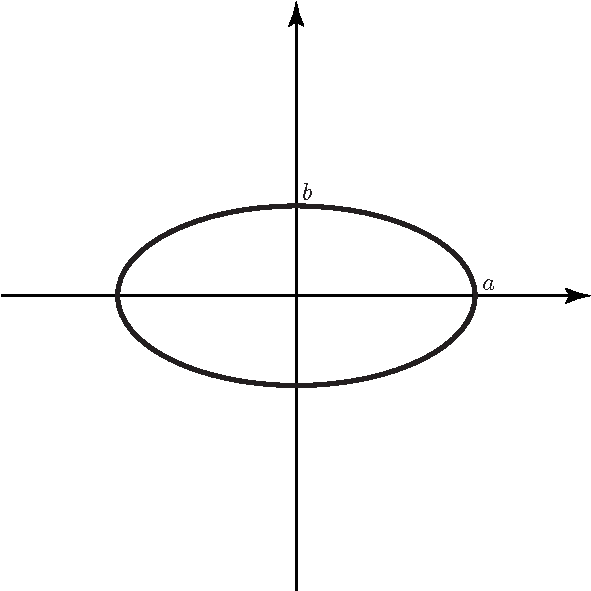
\includegraphics[trim=0cm 2.25cm 0cm 0cm, clip, scale=0.65]{images/ellisse.pdf}
\end{minipage}\hspace{-2mm}
\begin{minipage}{0.50\textwidth}
Dimostriamo finalmente la lunghezza dell'ellisse. Come è noto dal corso di \textsc{Analisi 2}, per una curva \textit{regolare} come l'ellisse è possibile calcolarne la lunghezza usando un'opportuna parametrizzazione.\\
Poniamo $a\geq b$ le lunghezze dei semiassi ed $e=\frac{\sqrt{a^2-b^2}}{a}\in\left[0,1\right)$ l'eccentricità. Una parametrizzazione è
\begin{equation*}
	\vec{r}\left(t\right)=\left(a\sin t,\ b\cos t\right)\quad t\in\left[0, 2\pi\right]
\end{equation*}
\end{minipage}\\
Allora
\begin{align*}
		L&=\int_{0}^{2\pi}\norm{\vec{r}'\left(t\right)}dt=\int_{0}^{2\pi}\norm{\left(a\cos t,\ -b\sin t\right)}dt=\int_{0}^{2\pi}\sqrt{a^2\cos^2t+b^2\sin^2t}dt=\\
		&=\int_{0}^{2\pi}\sqrt{a^2-\left(a^2+b^2\right)\sin^2t}dt=a\int_{0}^{2\pi}\sqrt{1-e^2\sin^2t}
\end{align*}
C'è un problema: la funzione $f\left(t\right)=\sqrt{1-e^2\sin^2t}$ non è \textbf{elementarmente integrabile}, cioè non ammette primitive in termini di funzioni elementari.
\begin{attention}
	Non essere elementarmente integrabile \textit{non} significa che non sia integrabile! La funzione integranda $f\left(t\right)$ è continua su $\left[0, 2\pi\right]$, dunque per il \textit{teorema fondamentale del calcolo integrale} ammette primitive su $\left[0, 2\pi\right]$. Una di esse è
	\begin{equation*}
		F\left(t\right)=\int_{0}^{t}\sqrt{1-e^2\sin^2y}dy\quad\forall y\in\left[0,2\pi\right]
	\end{equation*}
	Il problema è che \textit{non} possiamo riscrivere $F$ in modo esplicito usando \textit{solo} funzioni elementari.
\end{attention}
Questo tipo di integrale è detto \textbf{integrale ellittico}\index{integrale!ellittico}.
\begin{digression}
	Gli \textit{integrali ellittici} si incontrano in molti ambiti matematici. Ad esempio, appaiono nella risoluzione dell'equazione differenziale del moto di un pendolo semplice:
	\begin{equation*}
		\ddot{\theta}=-\frac{g}{l}\sin\theta
	\end{equation*}
	Sono il motivo per cui tale equazione si studia spesso per piccole oscillazioni, in modo da poter operare una linearizzazione $\sin\theta\sim\theta$ e calcolare il moto senza passare per tali integrali non calcolabili.\\
	Un altro esempio della loro importanza è noto agli appassionati di \textsc{Geometria}: infatti, la branca della Geometria Algebrica nasce anche dagli studi su tali integrali.
\end{digression}
Potremmo limitarci a considerare l'intero integrale ellittico come una nuova funzione, ma al più potremmo calcolarne il valore tramite metodi dell'\textsc{Analisi Numerica}. Invece, proviamo a riscrivere l'integrale utilizzando uno \textbf{sviluppo in serie} della funzione integranda.\\
Poniamo $x=-e^2\sin^2t$ e osserviamo che
\begin{equation*}
	\sqrt{1-e^2\sin^2 t}=\sqrt{1+x}=\left(1+x\right)^{\nicefrac{1}{2}}=\left(1+x\right)^\alpha\quad\text{dove }\alpha=\frac{1}{2}
\end{equation*}
Poichè $\left(1+x\right)^\alpha$ è una funzione di classe $\mathcal{C}^\infty$ in un intorno di $x=0$, si può approssimare localmente col \textbf{polinomio di Taylor}\index{polinomio di Taylor} di ordine $n$ centrato in $x=0$, $\forall n\geq 0$. Se il polinomio in questione è
\begin{equation*}
	P_{n,0}\left(x\right)=\sum_{j=0}^{n}\binom{\alpha}{j}x^j\quad\forall n\geq 0
\end{equation*}
con $\displaystyle\binom{\alpha}{j}$ il \textbf{coefficiente binomiale generalizzato}\index{coefficiente binomiale!generalizzato}\footnote{Nelle ‘‘Note aggiuntive'', a pagina \pageref{coefficientebinomialgeneralizzato} è possibile trovare la definizione e le proprietà del binomiale generalizzato.}, allora l'approssimazione dell'integranda data dal polinomio di Taylor è proprio
\begin{equation*}
	\left(1+x\right)^{\nicefrac{1}{2}}\approx\sum_{j=0}^{n}\binom{\nicefrac{1}{2}}{j}x^j\quad\forall n\geq 0
\end{equation*}
Risostituendo $x=-e^2\sin^2t$ abbiamo un'approssimazione dell'integranda. Tuttavia, noi vorremmo un \textit{risultato esatto}.\\
Sappiamo intuitivamente che più termini si hanno nello sviluppo di Taylor, più accurata è l'approssimazione; cosa succede per $n\to\infty$? Dobbiamo studiare la somma di serie
\begin{equation*}
	\sum_{j=0}^{+\infty}\binom{\nicefrac{1}{2}}{j}x^j
\end{equation*}
Già ci dobbiamo porre nuove domande: la serie \textit{converge} e per quali valori di $x$? Supponendo che la serie converga per opportuni valori di $x$, la serie converge proprio a $\left(1+x\right)^{\nicefrac{1}{2}}$?\\
\textit{In generale}, per $f\in\mathcal{C}^\infty$ qualsiasi \textbf{NO}, la serie di Taylor non converge proprio e se converge non converge ad $f$! Tuttavia, in questo caso siamo particolarmente fortunati: $\forall x\in \left(-1, 1\right)$ la serie converge\footnote{Nelle ‘‘Note aggiuntive'', a pagina XXX è possibile trovare la dimostrazione di tale convergenza.} e vale
\begin{equation*}
	\left(1+x\right)^{\frac{1}{2}}=\sum_{j=0}^{+\infty}\binom{\nicefrac{1}{2}}{j}x^j\quad\forall n\geq 0\quad \forall x\in\left(-1, 1\right)
\end{equation*}
In questa prima parte della dimostrazione abbiamo capito che è importante determinare quando è possibile passare dalla semplice \textit{approssimazione} di una funzione con il \textit{polinomio di Taylor} a poter riscrivere una funzione come una \textbf{serie di Taylor}\index{serie di Taylor} di funzioni opportune.
\subsection{La problematica dimostrazione della lunghezza dell'ellisse: passaggio al limite sotto segno di integrale}
Torniamo al problema originale. Ricordando che $x=-e^2\sin^2 t$, poiché $t\in\left[0,2\pi\right]$ si ha che $x\in\left[-e^2, 0\right]\subseteq\left(-1, 1\right)$ dato che $e^2<1$. Possiamo riscrivere l'integranda come il suo sviluppo in \textit{serie di Taylor}:
\begin{align*}
	\left(1-e^2\sin^2t\right)^{\nicefrac{1}{2}}=\sum_{j=0}^{+\infty}\binom{\nicefrac{1}{2}}{j}\left(-e^2\sin^2t\right)^j=\sum_{j=0}^{+\infty}\binom{\nicefrac{1}{2}}{j}\left(-1\right)^je^{2j}\sin^{2j}t\quad \forall t\in\left[0, 2\pi\right]
\end{align*}
Sostituiamo nell'integrale; poiché la funzione è pari e simmetrica, possiamo ricondurci a studiare l'integrale su $\left[0,\nicefrac{\pi}{2}\right]$:
\begin{equation*}
L=a\int_{0}^{2\pi}\left(1-e^2\sin^2t\right)^{\nicefrac{1}{2}}dt=4a\int_{0}^{\frac{\pi}{2}}\left(1-e^2\sin^2t\right)^{\nicefrac{1}{2}}dt=4a\int_{0}^{\frac{\pi}{2}}\sum_{j=0}^{+\infty}\binom{\nicefrac{1}{2}}{j}\left(-1\right)^je^{2j}\sin^{2j}tdt\squarequal
\end{equation*}
Incontriamo un nuovo problema: cos'è l'\textbf{integrale di una serie}? Se avessimo una somma di un numero \textit{finito} di termini per la \textit{linearità} dell'integrale potremmo scambiare la sommatoria con l'integrale, ma è possibile farlo nel caso di una serie?\\
Riscriviamo l'espressione precedente con la definizione di serie come \textit{limite} per $n\to +\infty$ delle \textit{ridotte}:
\begin{equation*}
	\squarequal 4a\int_{0}^{\frac{\pi}{2}}\lim_{n\to+\infty}\left(\sum_{j=0}^{n}\binom{\nicefrac{1}{2}}{j}\left(-1\right)^je^{2j}\sin^{2j}t\right)dt
\end{equation*}
Il problema precedente si può riformulare come \emph{‘‘È possibile scambiare integrale e limite?''}. Tale questione è come il problema del \textbf{passaggio al limite sotto segno di integrale}.\\
\textit{In generale}, la risposta è \textbf{NO}: non è possibile scambiare limite e integrale. Ciò nonostante anche questa volta siamo particolarmente fortunati e il passaggio è \textit{lecito}\footnote{Nelle ‘‘Note aggiuntive'', a pagina XXX è possibile trovare la dimostrazione che in questo caso il passaggio è lecito.} e si ha
\begin{align*}
	L&=4a\lim_{n\to+\infty}\int_{0}^{\frac{\pi}{2}}\sum_{j=0}^{n}\binom{\nicefrac{1}{2}}{j}\left(-1\right)^je^{2j}\sin^{2j}tdt\\
	&=4a\lim_{n\to+\infty}\sum_{j=0}^{n}\int_{0}^{\frac{\pi}{2}}\binom{\nicefrac{1}{2}}{j}\left(-1\right)^je^{2j}\sin^{2j}tdt\\
	&=4a\sum_{j=0}^{+\infty}\binom{\nicefrac{1}{2}}{j}\left(-1\right)^je^{2j}\int_{0}^{\frac{\pi}{2}}\sin^{2j}tdt
\end{align*}
Completando il calcolo dell'integrale\footnote{Nelle ‘‘Note aggiuntive'', a pagina XXX è possibile trovare tale calcolo.} si ottiene la formula della lunghezza scritta precedentemente.\\
\section{Non banali conseguenze di una domanda banale}
Abbiamo finalmente raggiunto una \textit{risposta}, seppur assolutamente non banale, alla domanda che ci eravamo posti originalmente: qual è la \textit{lunghezza dell'ellisse}? Nel far ciò ci siamo imbattuti in tutta una serie di problemi: esplicitare integrali non \textit{elementarmente} risolvibili, la \textit{convergenza} di \textit{serie di Taylor} di funzioni ad una funzione specifica, il \textit{passaggio al limite} sotto segno di \textit{integrale}.
La teoria matematica che tratteremo a partire dai capitoli successivi \textit{nasce} proprio da questi problemi apparsi nell'\textit{insidiosa ricerca} di una formula della lunghezza dell'ellisse.\\
In particolare, per capire quando era possibile il passaggio al limite sotto segno di integrale sono stati sviluppati diversi \textit{teoremi}, più o meno vantaggiosi da utilizzare, le cui ipotesi variano sensibilmente fra di loro: alcuni si inseriscono nella già nota \textit{teoria Riemanniana degli integrali}, mentre altri richiedono ipotesi completamente diverse. È da questi innumerevoli approcci al problema che, storicamente parlando, fu tale quesito a dare un \textit{impeto} fondamentale allo sviluppo della \textbf{teoria degli integrali di Lebesgue}.
\part{Convergenza di funzioni}
\labelPart{first}
% SVN info for this file
\svnidlong
{$HeadURL$}
{$LastChangedDate$}
{$LastChangedRevision$}
{$LastChangedBy$}

\chapter{Convergenza di funzioni}
\labelChapter{convergenzafunzioni}

\begin{introduction}
	‘‘BEEP BOOP QUESTA È UNA CITAZIONE.''
	\begin{flushright}
		\textsc{Marinobot,} dopo aver finito le citazioni stupide.
	\end{flushright}
\end{introduction}
\lettrine[findent=1pt, nindent=0pt]{L}{e} \textbf{[COMPLETARE]} % TO DO: completare l'intro
\section{Convergenza uniforme di funzioni}
Per poter trattare i problemi enunciati nel \refChapter{ellipseintroduction} dobbiamo parlare di convergenza di funzioni. Innanzitutto, ricordiamo le definizioni di distanza, spazio metrico e convergenza.
\begin{define}[Spazio metrico e distanza.]~{}\\
	Uno \textbf{spazio metrico}\index{spazio!metrico} è una coppia $\left(X,\ d\right)$ dove $X$ è un insieme e $\funz{d}{X\times X}{\realset^+}$ è una funzione detta \textbf{distanza}\index{distanza}, cioè tale che $\forall x,\ y,\ z\in X$ essa soddisfi le seguenti proprietà:
	\begin{enumerate}
		\item $\mvf{d}{x}{y}\geq 0,\ \mvf{d}{x}{y}=0\iff x=y$.
		\item $\mvf{d}{x}{y}=\mvf{d}{y}{x}$.
		\item $\mvf{d}{x}{y}\leq\mvf{d}{x}{z}+\mvf{d}{z}{y}$.
	\end{enumerate}
\end{define}
% OLD \begin{define}[Convergenza.]~{}\\
% più che convergenza metterei successione convergente rispetto a una distanza visto che dopo si fanno discorsi vari
% NEW
\begin{define}[Convergenza di successioni secondo la distanza.]~{}\\
	Una successione $v_n\in X$ \textbf{converge}\index{convergenza!di una successione} in $X$ a $v\in X$ se
	\begin{equation}
		\forall \epsilon >0,\ \exists N=N\left(\epsilon\right)\colon \forall n\geq N,\ \mvf{d}{v_n}{v}<\epsilon
	\end{equation}
\end{define}
Un \textit{caso particolare} di spazio metrico è lo spazio $X=\mathcal{C}\left(\left[a,b\right];\ \realset\right)$ delle funzioni continue su un intervallo compatto con la \textbf{metrica lagrangiana}\index{metrica!lagrangiana}:
\begin{equation}
	\mvf{d}{f}{g}=\max_{x\in\left[a,b\right]}\abs{f\left(x\right)-g\left(x\right)}
\end{equation}
\begin{observe}
	La distanza è ben definita perché la funzione $\abs{f\left(x\right)-g\left(x\right)}$, essendo definita su $\left[a,b\right]$ compatto, non si considera solo l'estremo superiore ma ammette massimo per il teorema di Weierstrass.
\end{observe}
\begin{define}[Convergenza nella metrica lagrangiana.]~{}\\
	Siano $f_n,\ f\in X$. Si dice che $f_n$ converge a $f$ in $X$ se
	\begin{equation}
		\forall \epsilon >0,\ \exists N=N\left(\epsilon\right)\colon \forall n\geq N,\ \max_{x\in\left[a,b\right]}\abs{f_n\left(x\right)-f\left(x\right)}<\epsilon
		\end{equation}
	\end{define}
	Siccome vale per il massimo allora vale per qualsiasi $x$, quindi la relazione si può riscrivere come
\begin{equation*}
	\forall \epsilon >0,\ \exists N=N\left(\epsilon\right)\colon \forall n\geq N,\ \abs{f_n\left(x\right)-f\left(x\right)}<\epsilon,\ \forall x\in\left[a,b\right]
\end{equation*}
\begin{observe}\label{convergenzalagrangianaeuniforme}
	La condizione, riscritta in questo modo, non solo \textit{non necessita} più dell'esistenza del \textit{massimo}, ma non è neanche necessario che l'intervallo sia \textit{compatto} o che le funzioni $f_n$ siano \textit{continue}: questa è in realtà una relazione \textit{più generale} rispetto alla semplice convergenza nella metrica lagrangiana!\\
%NEW
	Vedremo che nel caso di funzioni continue sui compatti la convergenza uniforme coincide con quella lagrangiana.
\end{observe}
\begin{define}[Convergenza uniforme.]~{}\\
	Siano $\funz{f_n,\ f}{A\subseteq\realset}{\realset}$ con $A\subseteq R$ qualsiasi. Si dice che $f_n$ \textbf{converge uniformemente}\index{convergenza!uniforme} a $f$\textbf{su} $A$ se
\begin{equation}
	\forall \epsilon >0,\ \exists N=N\left(\epsilon\right)\colon \forall n\geq N,\ \abs{f_n\left(x\right)-f\left(x\right)}<\epsilon,\ \forall x\in A
\end{equation}
\end{define}
\begin{define}[Funzione limite.]~{}\\
	Se $f_n$ converge uniformemente a $f$ su $A$, $f$ si dice \textbf{funzione limite}\index{funzione!limite}.
\end{define}
%OSS ho qualche dubbio che si dica funzione limite solo se la convergenza è uniforme
\begin{observe}
	Segue immediatamente dalla definizione che se $f_n$ converge uniformemente a $f$ su $A$, allora $\forall B\subseteq A$ si ha che $f_n$ converge uniformemente a $f$ su $B$.
\end{observe}
\begin{attention}
	È estremamente importante dire \textbf{dove} converge $f_n$: infatti, una stessa successione può convergere uniformemente su $A$, ma allo stesso tempo \textit{non convergere} uniformemente in un altro insieme $B$. Vedremo un esempio fondamentale a riguardo successivamente.
\end{attention}
Ora passiamo da questa definizione ad una formulazione equivalente \textit{operativa}.
Se essa vale per qualsiasi $x$ in $A$, allora vale per il $\sup$ e viceversa, quindi è equivalente a dire che
\begin{equation*}
	\forall \epsilon >0,\ \exists N=N\left(\epsilon\right)\colon \forall n\geq N,\ \sup_{x\in A}\abs{f_n\left(x\right)-f\left(x\right)}<\epsilon
\end{equation*}

Siccome il $\sup$ dipende da $n$, possiamo definire una successione $\displaystyle c_n\coloneqq\sup_{x\in A}\abs{f_n\left(x\right)-f\left(x\right)}\in\realset^+$. Allora la relazione sopra, per definizione di limite di una successione, è equivalente a $\displaystyle \lim_{n\to+\infty}c_n=0$, cioè
\begin{equation*}
\lim_{n\to+\infty}\left(\sup_{x\in A}\abs{f_n\left(x\right)-f\left(x\right)}\right)=0
\end{equation*}
In conclusione abbiamo mostrato che
\begin{equation}
	f_n\text{ converge uniformemente a }f\text{ in }A\iff\lim_{n\to+\infty}\left(\sup_{x\in A}\abs{f_n\left(x\right)-f\left(x\right)}\right)=0
\end{equation}
\begin{example}\label{valoreassolutoesempioconvergenzaassoluta}
	Proviamo che $f_n\left(x\right)=\sqrt{x^2+\frac{1}{n}}$ converge uniformemente a $f\left(x\right)=\abs{x}$ su $\realset$.\\
	Dobbiamo provare che
	\begin{equation*}
		\lim_{n\to+\infty}\left(\sup_{x\in \realset}\abs{f_n\left(x\right)-f\left(x\right)}\right)=0
	\end{equation*}
	\begin{enumerate}
		\item Calcoliamo il $\sup$ con $n$ \textit{fissato}:
		\begin{equation*}
			\sup_{x\in \realset}\abs{f_n\left(x\right)-f\left(x\right)}=\sup_{x\in \realset}\abs{\sqrt{x^2+\frac{1}{n}}-\abs{x}}=\sup_{x\in \realset}\left(\sqrt{x^2+\frac{1}{n}}-\abs{x}\right)
		\end{equation*}
		Per trovarlo tracciamo il grafico di $\phi_n\left(x\right)=\abs{\sqrt{x^2+\frac{1}{n}}-\abs{x}}$ e cerchiamo il suo estremo superiore. Per parità della funzione ci basta fare le nostre considerazioni su $\left(0,+\infty\right)$ per poi disegnare il resto del grafico grazie alla simmetria assiale rispetto all'asse $y$; studiando opportunamente la derivata e il limite all'infinito si ottiene il seguente grafico.
\begin{center}
	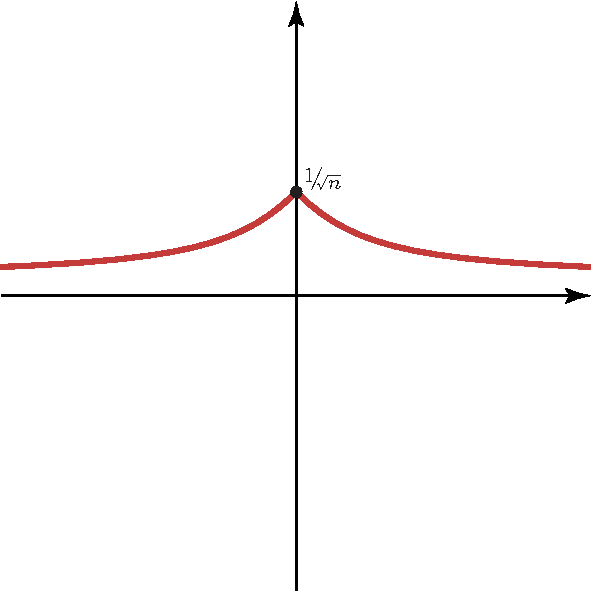
\includegraphics[trim=0cm 4cm 0cm 0cm, clip, scale=0.8]{images/grafico1.pdf}
\end{center}
		Segue chiaramente che
		\begin{equation*}
			\sup_{x\in \realset}\phi_n\left(x\right)=\phi_n\left(0\right)=\frac{1}{\sqrt{n}}\left( =c_n\right)
		\end{equation*}
	\item Calcoliamo il limite per $n\to +\infty$:
	\begin{equation*}
		\lim_{n\to+\infty}\left(\sup_{x\in A}\abs{f_n\left(x\right)-f\left(x\right)}\right)=\lim_{n\to+\infty}\frac{1}{\sqrt{n}}=0
	\end{equation*}
	\end{enumerate}
Abbiamo così verificato la convergenza richiesta.
\end{example}
%fINO A QUI
\begin{example}{\textsc{Successione geometrica.}}~{}\\
	Consideriamo $f_n\left(x\right)=x^n,\ \forall n\geq 0$. Allora:
	\begin{enumerate}
		\item $x^n$ converge uniformemente a $0$ su \textit{ogni} insieme $\left[-a,a\right],\ \forall a\colon 0<a<1$.
		\item $x^n$ \textbf{non} converge uniformemente a $0$ su $\left(-1,1\right)$.
	\end{enumerate}
\end{example}
\begin{demonstration}~{}\\
	\begin{enumerate}
		\item Sia $a\in\left(0,1\right)$ fissato e consideriamo
		\begin{equation*}
			\abs{x^n-0}=\abs{x^n}\implies\sup_{x\in \left[-a,a\right]}\abs{x^n-0}=\sup_{x\in \left[-a,a\right]}\abs{x^n}
		\end{equation*}
		Qual è il grafico di $x^n$?\\
		\begin{minipage}{0.75\textwidth}
			\begin{itemize}
				\item Se $n$ \textbf{pari}, è visivamente simile a quello di $x^2$.
			\end{itemize}
		\end{minipage}\hspace{-7mm}
		\begin{minipage}{0.15\textwidth}
			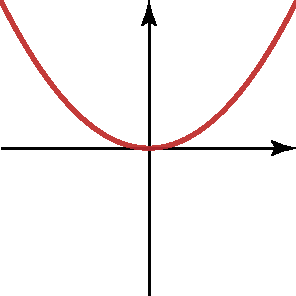
\includegraphics[trim=0cm 0cm 0cm 0cm, clip, scale=0.5]{images/grafico2a.pdf}
		\end{minipage}\\
			\begin{minipage}{0.75\textwidth}
		\begin{itemize}
			\item Se $n$ \textbf{dispari}, è visivamente simile a quello di $x^3$.
		\end{itemize}
	\end{minipage}\hspace{-7mm}
	\begin{minipage}{0.15\textwidth}
		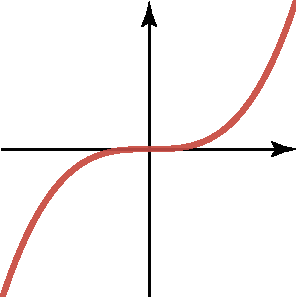
\includegraphics[trim=0cm 0cm 0cm 0cm, clip, scale=0.5]{images/grafico2b.pdf}
	\end{minipage}\\

		Tuttavia per $\abs{x^n},\ \forall n\geq 2$, che è una funzione pari, il grafico è visivamente simile a quello di $x^2$.
		Segue immediatamente che
		\begin{equation*}
			\sup_{x\in \left[-a,a\right]}\abs{x^n}=a^n,\ \forall a\colon 0<a<1
		\end{equation*}
		Ora si ha
		\begin{equation*}
			\lim_{n\to+\infty}\left(\sup_{x\in \left[-a,a\right]}\abs{x^n}\right)=\lim_{n\to+\infty}a^n=0
		\end{equation*}
		perché $a\in\left(0,1\right)$ e quindi $a^n$ è una successione geometrica convergente e pertanto il limite a $+\infty$ è sempre necessariamente 0.
		\item In questo caso
		\begin{equation*}
			\sup_{x\in\left(-1,1\right)}\abs{x^n}=1,\ \forall n
		\end{equation*}
		da cui
		\begin{equation*}
			\lim_{n\to+\infty}\left(\sup_{x\in\left(-1,1\right)}\abs{x^n}\right)=1\neq 0
		\end{equation*}
	pertanto \textit{non} c'è convergenza uniforme su $\left(-1,1\right)$.
	\end{enumerate}
\end{demonstration}
\subsection{Eserciziamoci! Convergenza uniforme}
\begin{exercise}
	$f_n\left(x\right)=\frac{x^n}{n}$ converge uniformemente a $0$ su $\left[0,1\right]$?
\end{exercise}
\begin{solution}
	Dimostriamo che
	\begin{equation*}
		\lim_{n\to+\infty}\left(\sup_{x\in \left[0,1\right]}\abs{\frac{x^n}{n}-0}\right)=\lim_{n\to+\infty}\left(\sup_{x\in \left[0,1\right]}\frac{x^n}{n}\right)=0
	\end{equation*}
	Poiché
	\begin{equation*}
		\sup_{x\in \left[0,1\right]}\frac{x^n}{n}=\frac{x^n}{n}\left.\right|_{x=1}\,=\frac{1}{n}
	\end{equation*}
	allora
	\begin{equation*}
	\lim_{n\to+\infty}\left(\sup_{x\in \left[0,1\right]}\frac{x^n}{n}\right)=\lim_{n\to+\infty}\frac{1}{n}=0
	\end{equation*}
\end{solution}
\subsection{Criterio di Cauchy per la convergenza uniforme}
Come nel caso delle successioni numeriche, esiste un \textbf{criterio di Cauchy} per la convergenza uniforme.
\begin{theorema}[Criterio di Cauchy per la convergenza uniforme.]~{}\\\label{criteriodicauchyperconvergenzauniforme}\index{criterio!di Cauchy!per la convergenza uniforme}
	Siano $\funz{f_n}{A\subseteq\realset}{\realset}$. Allora
	\begin{multline}
		f_n\text{ converge uniformemente su }A \iff\\
		\iff\forall \epsilon >0\ \exists N=N\left(\epsilon\right)\colon\forall n,m\geq N\ \abs{f_n\left(x\right)-f_m\left(x\right)}<\epsilon,\ \forall x\in A
	\end{multline}
\end{theorema}
\begin{observe}
Il criterio di Cauchy è un \textit{risultato teorico molto importante}, in quanto permette di mostrare la convergenza uniforme di una successione di funzioni \textit{senza sapere} quale sia il limite come invece è necessario nella definizione di convergenza, in modo analogo a ciò che succede con il criterio di Cauchy per le \textit{successioni numeriche}.
\end{observe}
\subsection{Visualizzazione della convergenza uniforme}
Siamo abituati alle successioni numeriche $v_n$ ed eventualmente a studiare il loro andamento in modo grafico, rappresentando sulle ascisse il numero $n$ e sulle ordinate il valore $v_n$. Nel caso di successioni di funzioni l'argomento è una funzione, quindi per studiarle può essere utile proprio disegnare i grafici degli $f_n$ e come convergono verso $f$.\\
Come appare \textit{visivamente} la convergenza uniforme? Possiamo riscrivere la condizione della convergenza uniforme
\begin{equation*}
	\forall \epsilon>0\ \exists N=N\left(\epsilon\right)\ \forall n\geq N\ \abs{f_n\left(x\right)-f\left(x\right)}<\epsilon,\ \forall x\in A
\end{equation*}
come
\begin{equation}
	f\left(x\right)-\epsilon<f_n\left(x\right)<f\left(x\right)+\epsilon,\ \forall x\in A\text{ definitivamente}
\end{equation}
In altre parole, $f_n$ deve essere compresa nell'\textbf{intorno tubulare} di $f\left(x\right)$ definitivamente, nel senso che le $f_n$ devono stare in questo intorno per ogni $n$ sufficientemente grande (cioè $\forall n\geq N$).
\begin{center}
	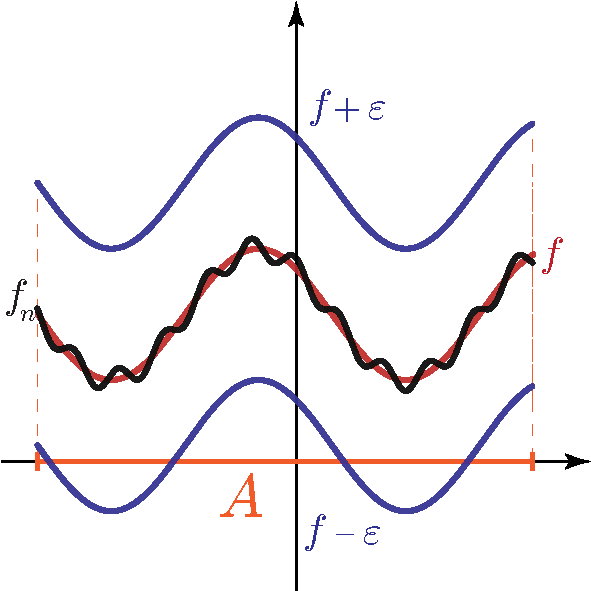
\includegraphics[trim=0cm 0cm 0cm 0cm, clip, scale=0.65]{images/grafico3.pdf}
\end{center}
\begin{define}[Intorno tubulare.]~{}\\
Un \textbf{intorno tubulare}\index{intorno!tubulare} di larghezza $\epsilon$ di una curva è l'unione di tutti i dischi di raggio $\epsilon$ con centro un punto di una curva.
\end{define}
\subsection{Generalizzazioni della convergenza uniforme}\label{sec:generalizzazioni-della-convergenza-uniforme}
Prima di tutto, ricordiamo le definizioni di norma e spazio normato.
\begin{define}[Spazio normato e norma.]~{}\\
	Uno \textbf{spazio normato}\index{spazio!normato} è una coppia $\left(X,\ \norm{\cdot}\right)$ dove $X$ è un spazio vettoriale su $\kamp$ reale o complesso e $\funz{\lvert\lvert\cdot\rvert\rvert}{X}{\realset^+}$ è una funzione detta \textbf{norma}\index{norma}, cioè tale che $\forall x,\ y\in X,\ \lambda\in\kamp$ essa soddisfi le seguenti proprietà:
	\begin{enumerate}
		\item $\norm{x}\geq 0,\ \norm{x}=0\iff x=0$.
		\item $\norm{\lambda x}=\abs{\lambda}\norm{x}$.
		\item $\norm{x+y}\leq\norm{x}+\norm{y}$.
	\end{enumerate}
\end{define}
	\begin{observe}
	Ogni spazio normato è anche uno spazio metrico se consideriamo la \textbf{metrica indotta dalla norma}\index{metrica!indotta dalla norma}, cioè la funzione data da $\mvf{d}{x}{y}\coloneqq\norm{x-y}$.
\end{observe}
Generalizziamo la definizione di convergenza uniforme considerando $\funz{f_n,\ f}{A}{Y}$, con $A$ \textit{insieme qualsiasi} e $Y$ uno spazio \textit{normato}; se vogliamo che valga anche il criterio di Cauchy è necessario che $Y$ sia \textit{anche} uno spazio \textbf{completo}.
\begin{define}[Successione di Cauchy.]~{}\\
		Una successione $v_n\in X$ è \textbf{di Cauchy}\index{successione!di Cauchy} in $X$ se
	\begin{equation}
		\forall \epsilon >0\ \exists N=N\left(\epsilon\right)\colon \forall n,m\geq N\ \mvf{d}{v_n}{v_m}<\epsilon
	\end{equation}
\end{define}
\begin{define}[Spazio completo.]~{}\\
	Uno spazio metrico è detto \textbf{completo}\index{spazio!metrico!completo} se tutte le successioni di Cauchy convergono.
\end{define}
\begin{observe}
	Una successione convergente è \textit{sempre} di Cauchy, ma in generale \textit{non tutte} le successioni di Cauchy convergono. L'implicazione opposta è vera solo se lo spazio è completo.
\end{observe}
Possiamo ora, date queste nuove ipotesi, riformulare la convergenza uniforme.
\begin{define}[Convergenza uniforme, generalizzata.]~{}\\
		Siano $\funz{f_n,\ f}{A}{Y}$ con $A$ insieme qualsiasi e $Y$ spazio normato (completo). Si dice che $f_n$ \textbf{converge uniformemente}\index{convergenza!uniforme} a $f$ \textbf{su} $A$ se
	\begin{equation}
		\forall \epsilon >0\ \exists N=N\left(\epsilon\right)\colon \forall n\geq N\ \norm{f_n\left(x\right)-f\left(x\right)}<\epsilon,\ \forall x\in A
	\end{equation}
\end{define}
\begin{digression}
	Volendo è possibile generalizzare ulteriormente parlando di convergenza uniforme per funzioni a valori in semplici \textbf{spazi metrici} (completi), sostituendo a $\norm{f_n\left(x\right)-f\left(x\right)}<\epsilon$ la condizione $\mvf{d}{f_n\left(x\right)}{f\left(x\right)}<\epsilon$. Nei nostri studi non affronteremo ciò e ci limiteremo a considerare il caso di spazi normati (completi).
\end{digression}
\section{Convergenza puntuale}
Durante gli studi di \textsc{Calcolo delle probabilità} si è parlato di tre tipi di convergenze di successioni di variabili aleatorie: la \textbf{convergenza in probabilità}, la \textbf{convergenza quasi certa} e la \textbf{convergenza in legge} (o in distribuzione). Consideriamo ora quest'ultima, di cui riportiamo la definizione.
\begin{define}[Convergenza in legge.]~{}\\
	Dato $\left(\Omega,\ \mathcal{M},\ \mathbb{P}\right)$ spazio di probabilità, $\funz{X_n,\ X}{\Omega}{\realset}$ variabili aleatorie e le due corrispettive \textit{funzioni di distribuzione}
	\begin{gather*}
		\funztot{F_n}{\realset}{\realset}{x}{F_n\left(x\right)=\mathbb{P}\left(X_n\leq x\right)\ \forall x\in \realset}\\
		\funztot{F}{\realset}{\realset}{x}{F_n\left(x\right)=\mathbb{P}\left(X\leq x\right)\ \forall x\in \realset}\\
	\end{gather*}
allora si dice che $X_n$ converge a $X$ \textbf{in legge}\index{convergenza!in legge} $\left(X_n\stackrel{d}{\to}X\right)$ se
\begin{equation}
	\lim_{n\to+\infty}F_n\left(x\right)=F\left(x\right),\ \forall x\in\realset\ \text{punto di continuità di }F.
\end{equation}
\end{define}
Quello che abbiamo appena scritta non è altro che il caso applicato agli \textit{studi probabilistici} della \textbf{convergenza puntuale} di una successione ad una funzione limite nel punto $x$.
\begin{define}[Convergenza puntuale.]~{}\\
	Siano $\funz{f_n,\ f}{A}{Y}$ con $A$ insieme qualsiasi e $Y$ spazio normato (completo). $f_n$ converge a $f$ \textbf{puntualmente}\index{convergenza!puntuale} in ogni punto di $A$ se
	\begin{equation}
		\forall x\in A\ \forall \epsilon>0\ \exists N=N\left(\epsilon,x\right)\colon\forall n\geq N\ \norm{f_n\left(x\right)-f\left(x\right)}<\epsilon
	\end{equation}
\end{define}
Confrontiamo qui $\funz{f_n,\ f}{A\subseteq R}{\realset}$:
\begin{enumerate}
	\item \textbf{(CU)} $f_n$ converge a $f$ \textbf{uniformemente} su $A$ se
	\begin{equation*}
		\forall \epsilon>0\ \exists N=N\left(\epsilon\right)\colon\forall n\geq N\ \abs{f_n\left(x\right)-f\left(x\right)}<\epsilon,\ \forall x\in A
	\end{equation*}
	\item \textbf{(CP)} $f_n$ converge a $f$ \textbf{puntualmente} in ogni punto di $A$ se
	\begin{equation*}
		\forall x\in A\ \forall \epsilon>0\ \exists N=N\left(\epsilon,x\right)\colon\forall n\geq N\ \abs{f_n\left(x\right)-f\left(x\right)}<\epsilon
	\end{equation*}
\end{enumerate}
Il quantificatore esistenziale $\exists$ implica che ciò che esiste dipende da tutto ciò che lo precede: nella convergenza puntuale $N$ non dipende dal solo $\epsilon$ come così capita nella \textbf{convergenza uniforme}, ma anche da $x$. La convergenza uniforme è più restrittiva rispetto alla puntuale.
\begin{observe}
	Questa differenza è concettualmente analoga a quella che c'è fra continuità uniforme e continuità.
\end{observe}
\begin{observe}
	Possiamo considerare $\forall \epsilon >0$ due punti $x'$ e $x''$ su cui valutare la \textbf{soglia} $N$ di un successione di funzioni: in questo caso abbiamo per il primo punto $N\left(\epsilon,\ x'\right)$ e per il secondo $N\left(\epsilon,\ x''\right)$. Vediamo subito che $\max\left(N\left(\epsilon,\ x'\right),N\left(\epsilon,\ x''\right)\right)$ è una soglia lecita sia per $x'$ sia $x''$.\\
	In generale, se voglio passare dalla convergenza puntuale alla convergenza uniforme devo considerare
	\begin{equation*}
		\sup_{x\in A}N\left(\epsilon, x\right)
	\end{equation*}
\begin{itemize}
	\item Se $A$ è finito, allora $\displaystyle\sup_{x\in A}N\left(\epsilon\right)=\max_{x\in A}N\left(\epsilon\right)=N\left(\epsilon\right)$ e c'è convergenza uniforme.
	\item Se $\displaystyle\sup_{x\in A}N\left(\epsilon\right)=+\infty$ allora \textit{non} c'è convergenza uniforme.
\end{itemize}
\end{observe}
Dalle definizioni segue immediatamente che
	\begin{multline}
	f_n\text{ converge uniformemente a }f\text{ in }A\implies\\
	\implies f_n\text{ converge puntualmente a }f\text{ in ogni punto di }A
\end{multline}
ma in generale vale che la convergenza puntuale \textbf{NON} implica la convergenza uniforme.
\begin{example}[Successione geometrica e convergenza puntuale.]~{}
	Consideriamo la successione geometrica $f_n\left(x\right)=x^n,\ \forall n\geq 0$.\\
	$\forall x\in\realset$ fissato si ha
	\begin{equation*}
		\lim_{n\to+\infty}x^n=
		\begin{cases}
			\begin{array}{ll}
				+\infty&\text{se }x>1\\
				1&\text{se }x=1\\
				0&\text{se }-1<x<1\\
				\text{non esiste}&\text{se }x\leq 1
			\end{array}
		\end{cases}
	\end{equation*}
Allora $x^n$ converge puntualmente a
\begin{equation*}
	f\left(x\right)=
	\begin{cases}
	1&\text{se }x=1\\
	0&\text{se }-1<x<1	
	\end{cases}
\end{equation*}
in ogni punto di $\left(-1,1\right]$.
\begin{center}
	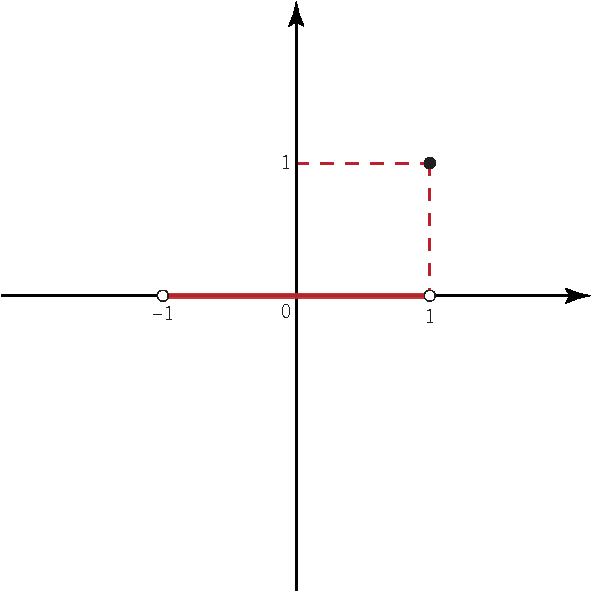
\includegraphics[trim=0cm 4cm 0cm 0cm, clip, scale=0.65]{images/grafico4.pdf}
\end{center}
\end{example}
Abbiamo provato precedentemente che $f_n\left(x\right)=x^n$ converge uniformemente a $f\equiv 0$ in ogni intervallo $\left[-a,a\right]\subsetneqq\left(-1,1\right),\ \forall a\in\left(0,1\right)$, ma \textit{non} converge uniformemente a $f=0$ in $\left(-1,1\right)$.\\
Questo mostra che su $\left(-1,1\right)$ c'è convergenza puntuale ma non uniforme.
\begin{observe}
	Questo esempio mostra inoltre che la CP \textit{non} è sufficiente in generale per trasferire la continuità alla funzione limite.
\end{observe}
\section{Proprietà di regolarità nel caso di convergenza uniforme e puntuale}
Adesso studiamo il diverso comportamento delle due tipologie di convergenza viste rispetto alle proprietà enunciate nel titolo di questa sezione: se le funzioni $f_n$ della successione sono limitate/continue/integrabili/differenziabile, la funzione limite $f$ è limitata/continua/integrabile/differenziabile?
\subsection{Limitatezza}
\begin{theorema}[Teorema di limitatezza per successioni.]~{}\\
Siano $\funz{f_n,f}{\left[a,b\right]}{\realset},\ n\geq 1$ tali che
\begin{enumerate}
	\item $f_n$ limitata su $\left[a,b\right],\ \forall n\geq 1$.
	\item $f_n$ converge uniformemente a $f$ su $\left[a,b\right]$.
\end{enumerate}
Allora $f$ è limitata su $\left[a,b\right]$.
\end{theorema}
\begin{demonstration}
	Dobbiamo provare che
	\begin{equation*}
		\exists n>0\colon \abs{f(x)}\leq n,\ \forall x\in A
	\end{equation*}
Per l'ipotesi $2)$ sappiamo che
\begin{equation*}
	\forall \epsilon>0\ \exists N=N\left(\epsilon\right)\colon\forall n\geq N\ \abs{f_n\left(x\right)-f\left(x\right)}<\epsilon,\ \forall x\in A
\end{equation*}
Posto ad esempio\footnote{La scelta di $\epsilon$ è assolutamente arbitraria.} $\epsilon = 2$, consideriamo la soglia $N_2=N\left(2\right)$ e $n=N_2$. Allora la relazione precedente risulta
\begin{equation*}
	\abs{f_{N_2}\left(x\right)-f\left(x\right)}<2,\ \forall x\in A
\end{equation*}
Consideriamo $f_{N_2}\left(x\right)$: per l'ipotesi $1)$ è limitata, cioè
\begin{equation*}
	\exists n_2>0\colon \abs{f_{N_2}(x)}\leq n,\ \forall x\in A
\end{equation*}
Per ogni $x\in A$ si ha quindi
\begin{equation*}
	\abs{f\left(x\right)}=\abs{f\left(x\right)+f_{N_2}(x)-f_{N_2}(x)}\leq\abs{f\left(x\right)-f_{N_2}(x)}+\abs{f_{N_2}(x)}\leq 2+n_2=n,\ \forall x\in A
\end{equation*}
\end{demonstration}
\begin{digression}
	Il risultato si generalizza ponendo $\funz{f_n,f}{X}{Y}$, dove $X$ è un qualunque insieme e $Y$ è uno spazio normato.
\end{digression}
La convergenza puntuale non è sufficiente per trasferire la limitatezza alla funzione limite: infatti, possiamo costruire un controesempio di una successione $f_n$ limitata che converge puntualmente ad una funzione non limitata.
\begin{example}
	Sia $\funz{f_n}{\left(0,1\right]}{\realset},\ n\geq1$, definita da
	\begin{equation*}
		f_n\left(x\right)=\begin{cases}
			\begin{array}{ll}
				n&\text{se }0<x<\frac{1}{n}\\
				\frac{1}{x}&\text{se }x\geq\frac{1}{n}\\
			\end{array}
		\end{cases}
	\end{equation*}
$\forall x\in \left(0,1\right]$.\\
Un grafico qualitativo di $f_n$ è rappresentato in figura.
\begin{center}
	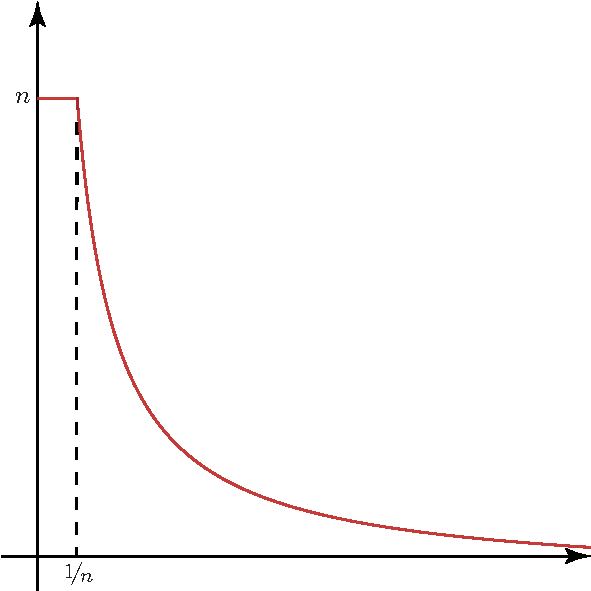
\includegraphics[trim=0cm 0cm 0cm 0cm, clip, scale=0.65]{images/grafico5.pdf}
\end{center}
Per ogni $n\geq1$ la funzione $f_n$ è limitata su $\left(0,1\right]$. Inoltre, $\forall x\in \left(0,1\right]$ si ha
	
	\begin{equation*}
		\lim_{n\to+\infty}f_n\left(x\right)=\frac{1}{x}
	\end{equation*}
	Infatti, fissato $x\in \left(0,1\right]$, indicando con le parentesi quadre la \textit{parte intera} e posto 
	\begin{equation*}
	n_x=\left[\frac{1}{x}\right]+1
	\end{equation*}
	allora se $n\geq n_x$ si ha $x>1/n$ e dunque
	\begin{equation*}
	f_n\left(x\right)=\frac{1}{x}
	\end{equation*}
	Si ha dunque
	\begin{equation*}
		\lim_{n\to+\infty}f_n\left(x\right)=\lim_{n\to+\infty}\frac{1}{x}=\frac{1}{x}
	\end{equation*}
	La successione di funzioni \textit{limitate} $f_n$ converge quindi puntualmente $\forall x\in \left(0,1\right]$ alla funzione $\frac{1}{x}$ che \textbf{non} è limitata su $\left(0,1\right]$.
\end{example}
\subsection{Continuità}
\begin{theorema}[Teorema di continuità per successioni.]~{}\\
	Siano $\funz{f_n,f}{\left[a,b\right]}{\realset},\ n\geq 1$ tali che
	\begin{enumerate}
		\item $f_n$ continua su $\left[a,b\right],\ \forall n\geq 1$.
		\item $f_n$ converge uniformemente a $f$ su $\left[a,b\right]$.
	\end{enumerate}
	Allora $f$ è continua su $\left[a,b\right]$.
\end{theorema}
\begin{demonstration}
	Sia $x_0\in\left[a,b\right]$ fissato. Dobbiamo dimostrare che
	\begin{equation*}
		\forall \epsilon>0\ \exists \delta>0 \colon \abs{x-x_0}<\delta\implies \abs{f\left(\right)-f\left(x_0\right)}<\epsilon
	\end{equation*}
	Per l'ipotesi $2)$ sappiamo che $f_n$ converge uniformemente; allora, fissato $\epsilon>0$, $\exists N=N\left(\epsilon\right)\in\naturalset$ tale che
	\begin{equation*}
		\abs{f_N\left(x\right)-f\left(x\right)}<\frac{\epsilon}{3},\ \forall x\in\left[a,b\right]
	\end{equation*}
Questa relazione chiaramente vale anche per $x_0$:
	\begin{equation*}
	\abs{f_N\left(x_0\right)-f\left(x_0\right)}<\frac{\epsilon}{3}
\end{equation*}
Per l'ipotesi $1)$ ogni $f_n$ è continua in $x_0$, in particolare $f_N$ la è. Per definizione di continuità, considerato sempre lo stesso $\epsilon>0$ di prima $\exists\delta >0$ tale che se $\abs{x-x_0}<\delta$ si ha
	\begin{equation*}
	\abs{f_N\left(x\right)-f_N\left(x_0\right)}<\frac{\epsilon}{3}
\end{equation*}
Quindi, se $\abs{x-x_0}<\delta$ abbiamo
\begin{equation*}
	\abs{f\left(x\right)-f\left(x_0\right)}\leq\abs{f\left(x\right)-f_N\left(x\right)}+\abs{f_N\left(x\right)-f_N\left(x_0\right)}+\abs{f_N\left(x_0\right)-f\left(x_0\right)}\leq\frac{\epsilon}{3}+\frac{\epsilon}{3}+\frac{\epsilon}{3}=\epsilon
\end{equation*}
\end{demonstration}
\begin{digression}
	Il risultato si generalizza ponendo $\funz{f_n,f}{X}{Y}$, dove $X$ è un qualunque insieme e $Y$ è uno spazio normato.
\end{digression}
La convergenza puntuale non è sufficiente per trasferire la continuità alla funzione limite: infatti, possiamo costruire un controesempio di una successione $f_n$ continua che converge puntualmente ad una funzione non continua.
\begin{example}
Consideriamo la successione geometrica $f_n(x)=x^n,\ n\geq1$, sull'intervallo $[0,1]$.\\
Sappiamo che essa converge puntualmente in ogni punto di $[0,1]$ alla funzione limite 
\begin{equation*}
	f\left(x\right)=
	\begin{cases}
		\begin{array}{ll}
			0&\text{se }0\geq x < 1\\
			1<&\text{se }x=1
		\end{array}
	\end{cases}
\end{equation*}
La successione di funzioni \textit{continue} $f_n$ converge quindi puntualmente per ogni $x\in[0,1]$ alla funzione $f$ che \textbf{non} è continua su $[0,1]$.
\end{example}
\subsection{Integrabilità e passaggio al limite sotto segno di integrale}
\begin{theorema}[Teorema di integrabilità per successioni, passaggio al limite sotto segno di integrale.]~{}\\
	Siano $\funz{f_n,f}{\left[a,b\right]}{\realset},\ n\geq 1$ tali che
	\begin{enumerate}
		\item $f_n\in\mathcal{R}\left(\left[a,b\right]\right),\ \forall n\geq 1$.
		\item $f_n$ converge uniformemente a $f$ su $\left[a,b\right]$.
	\end{enumerate}
	Allora
	\begin{enumerate}
		\item $f\in\mathcal{R}\left(\left[a,b\right]\right)$.
		\item Vale il \textbf{passaggio al limite sotto segno di integrale}\index{passaggio al limite sotto segno di integrale}:
		\begin{equation}
			\lim_{n\to+\infty}\int_{a}^{b}f_n\left(x\right)=\int_{a}^{b}lim_{n\to+\infty}f_n\left(x\right)dx=\int_{a}^{b}f\left(x\right)dx
		\end{equation}
	\end{enumerate}
\end{theorema}
Vedremo la dimostrazione di una versione più generica del teorema quando parleremo degli integrali di Lebesgue.\\
Per quanto questo teorema ha una notevole importanza, ha un campo d'azione particolarmente limitato. Infatti, anche cambiando leggermente le ipotesi non è più possibile affermare la tesi. Vediamo alcuni di questi controesempi.
\begin{example}
	La convergenza uniforme \textit{non} è sufficiente per trasferire alla funzione limite l'integrabilità su un intervallo \textit{illimitato}.\\
	Consideriamo la successione di funzioni $\funz{f_n}{\left[1,+\infty\right)}{\realset}$ definite da
\begin{equation*}
	f_n(x)=\frac{n}{nx+x^2},\ \forall x\geq1, n\geq1 
\end{equation*}
Per ogni $x\geq 1$ osserviamo che $f_n(x)\sim \frac{n}{nx}$ per $n\to+\infty$, quindi si ha
\begin{equation*}
	\lim_{n\to+\infty}f_n\left(x\right)=\lim_{n\to+\infty}\frac{n}{nx}=\frac{1}{x}
\end{equation*}
Si ha quindi convergenza puntuale in ogni punto di $\left[1,+\infty\right)$ alla funzione $f(x)=\frac{1}{x}$. Inoltre, la convergenza è uniforme su $\left[1,+\infty\right)$: vale infatti
\begin{equation*}
	\abs{f_n(x)-f(x)}=\abs{\frac{n}{nx+x^2}-\frac{1}{x}}=\frac{1}{n+x}
\end{equation*}
per ogni $x\geq1$, $n\geq1$. Per \textit{monotonia}, si ha quindi
\begin{equation*}
	\sup_{x\geq 1}\abs{f_n(x)-f(x)}=\sup_{x\geq1}\frac{1}{n+x}=\frac{1}{n+1},\ \forall n\geq1
\end{equation*}
Deduciamo che
\begin{equation*}
	\lim_{n\to+\infty}\left(\sup_{x\geq1}\abs{f_n(x)-f(x)}\right)=\lim_{n\to+\infty}\frac{1}{n+1}=0
\end{equation*}		
	da cui segue la convergenza uniforme su $\left[1,+\infty\right)$.
	Osserviamo ora che per ogni $n\geq1$ si ha
	\begin{equation*}
		f_n(x)\sim \frac{n}{x^2},\ x\to+\infty
	\end{equation*}
	e dunque $f_n$ è integrabile in senso improprio su $[1,+\infty)$, per ogni $n\geq1$; la funzione limite $f(x)=\frac{1}{x}$ \textit{non} è invece integrabile in senso improprio su $[1,+\infty)$.\\
	La successione di funzioni $f_n$ \textit{integrabili} su $[1,+\infty)$ converge quindi uniformemente su $[1,+\infty)$ alla funzione $f$ che \textbf{non} è integrabile su $[1,+\infty)$.
\end{example}
\begin{example}
	La convergenza uniforme \textit{non} è condizione necessaria per il passaggio al limite sotto segno di integrale.\\
	Consideriamo la successione di funzioni $f_n\left(x\right)=x^n$ definite su $\left[0,1\right]$. Osserviamo che
	\begin{equation*}
		\lim_{n\to+\infty}\int_{0}^{1}x^ndx=\lim_{n\to+\infty}\left[\frac{1}{n+1}x^{n+1}\right]_{0}^{1}=\lim_{n\to+\infty}\frac{1}{n+1}=0
	\end{equation*}
Invece, sappiamo che $x^n$ converge puntualmente in ogni punto di $[0,1]$ alla funzione limite 
\begin{equation*}
	f\left(x\right)=
	\begin{cases}
		\begin{array}{ll}
			0&\text{se }0\geq x < 1\\
			1<&\text{se }x=1
		\end{array}
	\end{cases}
\end{equation*}
dunque su $[0,1]$ $f\left(x\right)=\lim_{n\to\infty}f_n\left(x\right)$ è una funzione \textit{identicamente nulla} tranne un \textit{numero finito} di punti (in questo caso, uno soltanto). Allora
\begin{equation*}
	\int_{0}^{1}\lim_{n\to+\infty}x^ndx=\int_{0}^{1}0dx=0
\end{equation*}
 $x^n$ non converge uniformemente su $[\left[0,1\right]$, ma il passaggio al limite sotto segno di integrale si verifica comunque.
\end{example}
\begin{example}
	Consideriamo la successione di funzioni $f_n\left(x\right)=x^n$ definite su $\left[0,1\right]$. Osserviamo che
	\begin{equation*}
		\lim_{n\to+\infty}\int_{0}^{1}x^ndx=\lim_{n\to+\infty}\left[\frac{1}{n+1}x^{n+1}\right]_{0}^{1}=\lim_{n\to+\infty}\frac{1}{n+1}=0
	\end{equation*}
	Invece, sappiamo che $x^n$ converge puntualmente in ogni punto di $[0,1]$ alla funzione limite 
	\begin{equation*}
		f\left(x\right)=
		\begin{cases}
			\begin{array}{ll}
				0&\text{se }0\geq x < 1\\
				1<&\text{se }x=1
			\end{array}
		\end{cases}
	\end{equation*}
	dunque su $[0,1]$ $f\left(x\right)=\lim_{n\to\infty}f_n\left(x\right)$ è una funzione \textit{identicamente nulla} tranne un \textit{numero finito} di punti (in questo caso, uno soltanto). Allora
	\begin{equation*}
		\int_{0}^{1}\lim_{n\to+\infty}x^ndx=\int_{0}^{1}0dx=0
	\end{equation*}
	$x^n$ non converge uniformemente su $[\left[0,1\right]$, ma il passaggio al limite sotto segno di integrale si verifica comunque.
\end{example}
\begin{example}
	La convergenza uniforme \textit{non} è condizione sufficiente per il passaggio al limite sotto il segno di integrale nel caso in un intervallo \textit{illimitato}.
	Sia $\funz{f_n}{\left[0,+\infty\right)}{\realset}$, $n\geq1$, definita da
	\begin{equation*}
		f_n\left(x\right)=\begin{cases}
			\begin{array}{ll}
				\frac{1}{n}&\text{se }n\geq x\geq2n\\
				\frac{1}{x}&\text{se }x<n\vee x>2n
			\end{array}
		\end{cases}
	\end{equation*}
Osserviamo che
\begin{align*}
	\lim_{n\to+\infty}\int_{0}^{+\infty}f_n\left(x\right)dx=&\lim_{n\to+\infty}\left[\int_{0}^{n}0dx+\int_{n}^{2n}\frac{1}{n}dx+\int_{2n}^{+\infty}0dx\right]=\lim_{n\to+\infty}\int_{n}^{2n}\frac{1}{n}dx=\\
	=&\lim_{n\to+\infty}\left[\frac{x}{n}\right]_{n}^{2n}=\lim_{n\to+\infty}\frac{2n--n}{n}=\lim_{n\to+\infty}1=1
\end{align*}
Invece, si vede immediatamente che
	\begin{equation*}
	\int_{0}^{+\infty}\lim_{n\to+\infty}f_n\left(x\right)dx=\int_{0}^{+\infty}0dx=0
\end{equation*}
Vediamo che $f_n$ converge uniformemente su $\left[0,+\infty\right)$ a $0$:
\begin{gather*}
	\sup_{x\in\left[0,+\infty\right)}\abs{f_n\left(x\right)-f\left(x\right)}=\frac{1}{n}\\
	\lim_{n\to+\infty}\left(\sup_{x\in\left[0,+\infty\right)}\right)=\lim_{n\to+\infty}\frac{1}{n}=0
\end{gather*}
Anche aggiungendo al teorema l'ipotesi che $f\left(x\right)$ sia Riemann-integrabile (in questo caso ciò è verificato), il passaggio al limite sotto segno di integrale \textit{non} si verifica \textit{necessariamente} se l'intervallo è illimitato.
\end{example}
\begin{example}
	La convergenza puntuale \textit{non} è condizione sufficiente per il passaggio al limite sotto il segno di integrale, nemmeno nel caso di un intervallo limitato.
	Consideriamo la successione di funzioni $f_n\left(x\right)=nx\left(1-x^2\right)^n$ definite su $\left[0,1\right]$. Osserviamo che
	\begin{align*}
		\lim_{n\to+\infty}\int_{0}^{1}nx\left(1-x^2\right)^ndx=&-\frac{1}{2}\lim_{n\to+\infty}\int_{0}^{1}n\left(-2x\right)\left(1-x^2\right)^n=\\
		=&-\frac{1}{2}\lim_{n\to+\infty}n\left[\frac{1}{n+1}\left(1-x^2\right)^{n+1}\right]_{0}^{1}=\frac{1}{2}\lim_{n\to+\infty}\frac{n}{n+1}=\frac{1}{2}
	\end{align*}
Invece, osserviamo che, fissato $x$ rispetto alla $n$ $nx\left(1-x^2\right)^n=x\frac{\left(1-x^2\right)^n}{\frac{1}{n}}$ si può vedere come il rapporto di un esponenziale di ragione (in modulo) minore di 1 con il reciproco di un termine lineare, dunque per $n\to+\infty$ l'esponenziale tende a $0$ molto più velocemente di $\frac{1}{n}$: segue che
	\begin{equation*}
	\int_{0}^{1}\lim_{n\to+\infty}nx\left(1-x^2\right)^ndx=\int_{0}^{1}0dx=0
\end{equation*}
Per lo stesso ragionamento si vede che $f_n\left(x\right)$ converge puntualmente a $0$ per ogni punto di $\left[0,1\right]$, ma \textit{non} si verifica il passaggio al limite sotto segno di integrale.
\end{example}
\subsection{Derivabilità}
Date $\funz{f_n,f}{A\subseteq\realset}{\realset}$ con $f$ la funzione limite di $f_n$ su $A$, possiamo porci due domande:
\begin{enumerate}
	\item $f_n$ derivabile su $A\implies f$ derivabile su $A$?
	\item Vale lo scambio tra derivata e limite?
	\begin{equation*}
		\lim_{n\to+\infty}f'_n\left(x\right)=D\left(\lim_{n\to+\infty}f\left(x\right)\right)
	\end{equation*}
	O, in altre parole, il diagramma seguente è commutativo?
	% https://q.uiver.app/?q=WzAsNCxbMCwwLCJmX24iXSxbMSwwLCJmJ19uIl0sWzAsMSwiXFxsaW1fe25cXHRvK1xcaW5mdHl9Zl9uIl0sWzEsMSwiXFxsaW1fe25cXHRvK1xcaW5mdHl9ZidfbiJdLFswLDEsIkQiXSxbMCwyLCJcXGxpbSIsMl0sWzEsM10sWzIsM11d
\[\begin{tikzcd}
	{f_n} & {f'_n} \\
	{\textcolor{blueill}{\displaystyle\lim_{n\to+\infty}f_n}} & {\displaystyle\lim_{n\to+\infty}f'_n}
	\arrow["D", from=1-1, to=1-2]
	\arrow["\lim"', color={rgb,255:red,46;green,49;blue,146}, from=1-1, to=2-1]
	\arrow["\lim", from=1-2, to=2-2]
	\arrow["D"', color={rgb,255:red,46;green,49;blue,146}, from=2-1, to=2-2]
\end{tikzcd}\]
\end{enumerate}
La risposta ad entrambe domande, a differenza di quanto ci si potrebbe aspettare dati i risultati su limitatezza/continuità/integrabilità, è \textbf{NO}, anche nel caso di \textit{convergenza uniforme}.
\begin{example}
	La convergenza uniforme \textit{non} è condizione sufficiente per trasferire alla funzione limite la derivabilità.\\
	Consideriamo la successione $f_n(x)=\sqrt{x^2+\frac{1}{n}},\ \forall x\in \realset,\ \forall n\geq1$.
	\begin{itemize}
		\item $f_n$ è derivabile.
		\item $f_n$ abbiamo visto\footnote{Si veda pag. \pageref{valoreassolutoesempioconvergenzaassoluta}, sezione \ref{valoreassolutoesempioconvergenzaassoluta}.} converge uniformemente su $\realset$ a $f\left(x\right)=\abs{x}$ che \textit{non} è derivabile in $x=0$.
	\end{itemize}
\end{example}
\begin{example}
	La convergenza uniforme \textit{non} è condizione sufficiente per poter scambiare limite e derivata, anche se si aggiunge l'ipotesi che la funzione limite sia derivabile.\\
	Consideriamo la successione $f_n(x)=\frac{sin\left(nx\right)}{\sqrt{n}},\ \forall x\in \realset,\ \forall n\geq1$.
	\begin{itemize}
		\item $f_n$ è derivabile su $\realset$, $\forall n\geq 1$, e vale
		\begin{equation*}
			f'\left(x\right)=\sqrt{n}\cos\left(nx\right),\ \forall x\in \realset,\ \forall n\geq1
		\end{equation*}
		\item
		\begin{itemize}
			\item $f_n$ converge \textbf{puntualmente} a $f\left(x\right)=0,\ \forall x\in\realset$:
			\begin{equation*}
				\lim_{n\to+\infty}f_n\left(x\right)=\lim_{n\to+\infty}\underbrace{\frac{1}{\sqrt{n}}}_{\to 0}\underbrace{\sin\left(nx\right)}_{\text{limitato}}=0,\ \forall x\in\realset
			\end{equation*}
			\item $f_n$ converge \textbf{uniformemente} a $f\left(x\right)=0,\ \forall x\in\realset$:
			\begin{equation*}
				\lim_{n\to+\infty}\left(\sup_{x\in\realset}\abs{f_n\left(x\right)-f\left(x\right)}\right)=\lim_{n\to+\infty}\left(\sup_{x\in\realset}\abs{\frac{\sin\left(nx\right)}{\sqrt{n}}}\right)=\lim_{n\to+\infty}\frac{1}{\sqrt{n}}=0
			\end{equation*}
		\end{itemize}
		Osserviamo che in entrambi i casi $f\left(x\right)=0$ su $\realset$: questa funzione è chiaramente derivabile e vale
		\begin{equation*}
			D\left(\lim_{n\to+\infty}f_n\left(x\right)\right)=D\left(0\right)=0,\ \forall x\in\realset
		\end{equation*}
	D'altro canto, si ha
	\begin{equation*}
			\lim_{n\to+\infty}D\left(f_n\left(x\right)\right)=\lim_{n\to+\infty}f'_n\left(x\right)=\lim_{n\to+\infty}\sqrt{n}\cos\left(nx\right)
	\end{equation*}
		Ad esempio, per $x=0$ troveremmo
		\begin{equation*}
				\lim_{n\to+\infty}D\left(f_n\left(x\right)\right)=\lim_{n\to+\infty}\sqrt{n}=+\infty
		\end{equation*}
	Quindi non si può per $x=0$ scambiare limite e derivata-
	\end{itemize}
\end{example}
Esiste comunque un legame tra \textit{successioni di funzioni}, \textit{derivabilità} e convergenza uniforme; scopriamo che non è più la successione $f_n$ a convergere uniformemente, bensì sono le derivate $f'$ della successioni a doverlo fare.
\begin{theorema}[Teorema di derivabilità per successioni.]~{}\\
	Siano dati $\funz{f_n}{\left(a,b\right)}{\realset}$ tali che
	\begin{enumerate}
		\item $f_n$ derivabili su $\left(a,b\right)$.
		\item $\exists c\in\left(a,b\right)\colon f_n\left(c\right)$ converge puntualmente.
		\item $f'_n$ converge uniformemente a $g$ su $\left(a,b\right)$.
	\end{enumerate}
Allora
\begin{enumerate}
	\item $\exists\funz{f}{\left(a,b\right)}{\realset}$ tale che $f_n$ converge uniformemente a $f$ su $\left(a,b\right)$.
	\item $f$ è derivabile.
	\item $f'\left(x\right)=g\left(x\right),\ \forall x\in \left(a,b\right)$, ossia
	\begin{equation}
		f'\left(x\right)=\lim_{n\to+\infty}f'_n\left(x\right),\ \forall x\in\left(a,b\right)
	\end{equation}
\end{enumerate}
\end{theorema}
Per dimostrare il teorema, faremo uso di tre strumenti: il \textit{criterio di Cauchy per la convergenza uniforme} (teorema \ref{criteriodicauchyperconvergenzauniforme}, pag. \pageref{criteriodicauchyperconvergenzauniforme}), il \textit{teorema di scambio di limiti} e una conseguenza \textit{teorema di Lagrange}. Enunciamo questi ultimi due.
\begin{theorema}[Teorema di scambio di limiti.]~{}\\
	Dati $\funz{g_n,g}{I\subseteq \realset}{\realset}$ e $c$ punto di accumulazione di $I$, se
	\begin{enumerate}
		\item $g_n$ converge \textit{uniformemente} a $g$ su $I$
		\item Per ogni $n \geq 1$ esiste $L_n\in\realset$ tale che
		\begin{equation*}
			\lim_{x\to c}g_n\left(x\right)=L_n
		\end{equation*}
	\end{enumerate}
	Allora:
	\begin{enumerate}
		\item Esistono finiti
		\begin{equation}
				\lim_{x\to c}g\left(x\right),\qquad\lim_{n\to+\infty}L_n
		\end{equation}
		\item Vale la relazione
		\begin{equation}
			\lim_{x\to c}g\left(x\right)=\lim_{n\to+\infty}L_n
		\end{equation}
		ossia
	\begin{equation}
		\lim_{x\to c}\lim_{n\to+\infty}g_n\left(x\right)=\lim_{n\to+\infty}\lim_{x\to c}g_n\left(x\right)
	\end{equation}
	\end{enumerate}
	
\end{theorema}
\begin{corollary}[Conseguenza al teorema di Lagrange.]~{}\\
Sia $\funz{h}{\left(\alpha,\beta\right)\subseteq\realset}{\realset}$ derivabile in $\left(\alpha,\beta\right)$. Allora:
\begin{equation}
	\forall u,v\in\left(\alpha,\beta\right)\colon\abs{h\left(u\right)-h\left(v\right)}\leq\left(\sup_{x\in\left(\alpha,\beta\right)}\abs{h'\left(x\right)}\right)\abs{u-v}
\end{equation}
\end{corollary}
\begin{demonstration} \textsc{(del Teorema di derivabilità per successioni.)}
\begin{enumerate}
	\item Dimostriamo la \textit{convergenza uniforme} di $f_n$ su $\left(a, b\right)$. Per il Criterio di Cauchy per la convergenza uniforme è sufficiente
	dimostrare che
	\begin{equation*}
		\forall \epsilon >0\ \exists N=N\left(\epsilon\right)\colon\forall n,m\geq N\ \sup_{x\in \left(a,b\right)}\abs{f_n\left(x\right)-f_m\left(x\right)}<\epsilon
	\end{equation*}
Sia $\epsilon>0$. Per ogni $x\in\left(a,b\right)$, preso $c$ come da ipotesi $2)$:
\begin{equation*}
	\abs{f_n\left(x\right)-f_m\left(x\right)}\leq \abs{f_n\left(x\right)-f_m\left(x\right)-\left(f_n\left(c\right)-f_m\left(c\right)\right)}+\abs{f_n\left(c\right)-f_m\left(c\right)}
\end{equation*}
Studiamo il \textit{primo addendo}. Per il \textit{corollario al teorema di Lagrange} si ha
\begin{equation*}
	\abs{f_n\left(x\right)-f_m\left(x\right)-\left(f_n\left(c\right)-f_m\left(c\right)\right)}\leq\left(\sup_{t\in\left(a,b\right)}\abs{x-c}\right)
\end{equation*}
Inoltre, poiché per ipotesi $3)$ $f'_n$ converge uniformemente su $\left(a,b\right)$, si ha per il criterio di Cauchy che
\begin{equation*}
	\forall \epsilon >0\ \exists N_1=N_1\left(\epsilon\right)\colon\forall n,m\geq N_1\ \sup_{x\in \left(a,b\right)}\abs{f'_n\left(x\right)-f'_m\left(x\right)}<\frac{\epsilon}{2\left(b-a\right)}
\end{equation*}
Segue dunque che
\begin{align*}
	\abs{f_n\left(x\right)-f_m\left(x\right)-\left(f_n\left(c\right)-f_m\left(c\right)\right)}&\leq\left(\sup_{t\in\left(a,b\right)}\abs{x-c}\right)\leq\\
	&\leq\frac{\epsilon}{2\left(b-a\right)}\abs{x-c}\leq\frac{\epsilon}{2},\ \forall x\in\left(a,b\right),\ \forall n,m\geq N_1
\end{align*}
Per il \textit{secondo addendo}, dato che per ipotesi $2)$ $f_n$ converge puntualmente in $c$, possiamo applicare il criterio di Cauchy per le successioni:
\begin{equation*}
		\forall \epsilon >0\ \exists N_2=N_2\left(\epsilon\right)\colon\forall n,m\geq N_2\ \abs{f_n\left(c\right)-f'_m\left(c\right)}<\frac{\epsilon}{2}
\end{equation*}
Posto $N=\max\left\{N_1,N_2\right\}$, per ogni $n,m\geq N$ si ha
\begin{align*}
	\abs{f_n\left(x\right)-f_m\left(x\right)}&\leq \abs{f_n\left(x\right)-f_m\left(x\right)-\left(f_n\left(c\right)-f_m\left(c\right)\right)}+\abs{f_n\left(c\right)-f_m\left(c\right)}<\\
	&<\frac{\epsilon}{2}+\frac{\epsilon}{2}=\epsilon,\ \forall x\in\left(a,b\right)
\end{align*}
	Da cui segue:
	\begin{equation*}
		\sup_{x\in\left(a,b\right)}\abs{f_n\left(x\right)-f_m\left(x\right)}<\epsilon,\ \forall n,m\geq N
	\end{equation*}
\item Denominiamo $f$ il limite \textit{puntuale} di $f_n$, che esiste e coincide con quello uniforme per la dimostrazione appena fatta al punto $1)$. Riscriviamo la tesi $2)$ e $3)$ nella seguente maniera:
\begin{enumerate}
	\setcounter{enumii}{1}
	\item Per ogni $d\in\left(a,b\right)$ vale $\displaystyle\lim_{x\to d}\frac{f\left(x\right)-f\left(d\right)}{x-d}$
	\item $\displaystyle\lim_{x\to d}\lim_{n\to+\infty}\frac{f_n\left(x\right)-f_n\left(d\right)}{x-d}=\lim_{n\to+\infty}\lim_{x\to d}\frac{f_n\left(x\right)-f_n\left(d\right)}{x-d}$.
\end{enumerate}
Verifichiamo le ipotesi del \textit{teorema di scambio dei limiti}:
\begin{itemize}
	\item $\displaystyle\lim_{x\to d}\frac{f_n\left(x\right)-f_n\left(d\right)}{x-d}$ esiste \textit{finito} in quanto per ipotesi $1)$ gli $f_n$ sono \textit{derivabili} su $\left(a,b\right)$.
	\item $\frac{f_n\left(x\right)-f_n\left(d\right)}{x-d}$ conv\textit{erge uniformemente} su $\left(a,b\right)\setminus\left\{d\right\}$.\\
	Infatti, per ogni $\epsilon>0$ e per ogni $x\in\left(a,b\right)\setminus\left\{d\right\}$ si ha, in virtù del \textit{corollario al teorema di Lagrange}
	\begin{align*}
		\abs{\frac{f_n\left(x\right)-f_n\left(d\right)}{x-d}-\frac{f_m\left(x\right)-f_m\left(d\right)}{x-d}}&\leq\abs{\frac{f_n\left(x\right)-f_m\left(x\right)-\left(f_n\left(d\right)-f_m\left(d\right)\right)}{x-d}}\leq\\
		&\leq\sup_{t\in\left(a,b\right)}\abs{f'_n\left(t\right)-f'_m\left(t\right)}
	\end{align*}
Inoltre, si applica il \textit{criterio di Cauchy} alle successione $f'_n$: per ogni $\epsilon>0\ \exists N=N_0$ tale che per ogni $\forall n,m\geq N$ vale
\begin{equation*}
	\sup_{t\in\left(a,b\right)}\abs{f'_n\left(t\right)-f'_m\left(t\right)}<\epsilon
\end{equation*}
da cui segue
\begin{equation*}
	\abs{\frac{f_n\left(x\right)-f_n\left(d\right)}{x-d}-\frac{f_m\left(x\right)-f_m\left(d\right)}{x-d}}<\epsilon,\ \forall x\in\left(a,b\right)\setminus\left\{d\right\}
\end{equation*}
\end{itemize} 
Per il \textit{criterio di Cauchy} sulla convergenza uniforme, c'è convergenza uniforme su $\left(a,b\right)\setminus\left\{d\right\}$. Il teorema di scambio dei limiti garantisce che il limite
\begin{equation*}
	\lim_{x\to d}\lim_{n\to+\infty}\frac{f_n\left(x\right)-f_n\left(d\right)}{x-d}\iff\lim_{x\to d}\frac{f\left(x\right)-f\left(d\right)}{x-d}
\end{equation*}
esiste \textit{finito} (tesi $2$) e vale lo \textit{scambio di limite e derivata} (tesi $3$).
\end{enumerate}
\end{demonstration}
% SVN info for this file
\svnidlong
{$HeadURL$}
{$LastChangedDate$}
{$LastChangedRevision$}
{$LastChangedBy$}

\chapter{Serie di funzioni}
\labelChapter{seriefunzioni}

\begin{introduction}
	‘‘BEEP BOOP QUESTA È UNA CITAZIONE.''
\begin{flushright}
	\textsc{Marinobot,} dopo aver finito le citazioni stupide.
\end{flushright}
\end{introduction}
\lettrine[findent=1pt, nindent=0pt]{L}{e} Nel \refChapter{convergenzafunzioni} abbiamo iniziato a trattare la convergenza uniforme e puntuale di successioni di funzioni. Adesso passiamo a parlare di serie di funzioni.
\textbf{[COMPLETARE]} % TO DO: completare l'intro
\section{Serie in spazio normato}
Innanzitutto, ricordiamo le definizioni di serie a valori reali e di convergenza (assoluta) di una serie a valore reali.
\begin{define}[Serie a valori reali e convergenza di una serie.]~{}\\
	Data una successione $x_n\in\realset$, $n\geq 0$, la \textbf{serie}\index{serie} $\displaystyle\sum_{k=0}^{+\infty}x_k$ è la somma di tutti gli elementi della successione.\\
	Considerata la \textit{somma parziale}, o altresì detta \textbf{ridotta}\index{ridotta}
	\begin{equation}
		s_n=\sum_{k=0}^{n}x_k\quad\forall n\geq 0
	\end{equation}
si dice che la serie $\displaystyle\sum_{k=0}^{+\infty}x_k$ \textbf{converge}\index{convergenza!di una serie}\seeonlyindex{convergenza!di una serie}{convergenza!semplice} se converge la successione $s_n$; si pone in tal caso
\begin{equation}
	\sum_{k=0}^{+\infty}x_k=\lim_{n\to+\infty}s_n
\end{equation}
\end{define}
\begin{define}[Convergenza assoluta.]~{}\\
	Sia $x_n$ una successione a valori reali. La serie $\displaystyle\sum_{k=0}^{+\infty}x_k$ \textbf{converge assolutamente}\seeonlyindex{convergenza!totale}{convergenza!assoluta} in $\realset$ se converge la serie $\displaystyle\sum_{k=0}^{+\infty}\abs{x_k}$.
\end{define}
\begin{theorema}[Convergenza assoluta implica convergenza semplice.]~{}\\\label{teoremaassimplicasemplice}
	Ogni serie di numeri reali assolutamente convergente è anche semplicemente convergente.
\end{theorema}
\begin{demonstration}
	% TO DO: guarda moodle per la dimostrazione
\end{demonstration}
\begin{observe}\label{convergenzaassolutadipendedacauchy}
	Il teorema appena dimostrato è una conseguenza della \textbf{completezza} di $\realset$. Infatti, abbiamo usato il \textit{criterio di Cauchy}, che si basa sul fatto che le successioni di Cauchy convergono sempre in $\realset$ e quindi proprio per la completezza dei reali.
\end{observe}
Il viceversa del teorema appena dimostrato non è valido, come segue dal seguente controesempio.
\begin{example}
	Consideriamo la serie $\displaystyle\sum_{n=1}^{+\infty}\left(-1\right)^n\frac{1}{n}$: non converge assolutamente in quanto la serie, con gli elementi in modulo, diventa
	\begin{equation*}
		\sum_{n=1}^{+\infty}\abs{\left(-1\right)^n\frac{1}{n}}=\sum_{n=1}^{+\infty}\frac{1}{n}
	\end{equation*}
	che, essendo la \textbf{serie armonica}\footnote{Nelle ‘‘Note aggiuntive'', a pagina XXX è possibile trovare maggiori dettagli sulle serie notevoli.}, non converge. Tuttavia, la serie semplice è una serie a segni alterni e poiché
	\begin{itemize}
		\item $\frac{1}{n}$ è decrescente $\forall n\geq 1$.
		\item $\displaystyle\lim_{n\to+\infty}\frac{1}{n}=0$.
	\end{itemize} 
	per il \textit{criterio di Leibniz} la serie semplice converge. Pertanto, la convergenza semplice non implica la convergenza assoluta.
\end{example}
Prendiamo ora $x_n\in X$, con $X$ un insieme generico. Per generalizzare la definizione di serie convergente abbiamo bisogno che su $X$ si possano compiere i seguenti passaggi:
\begin{itemize}
	\item Poter definire $s_n$, cioè è necessario \textit{sommare} elementi di $X$.
	\item Poter definire la \textit{convergenza} in $X$.
\end{itemize}
Se dotiamo l'insieme $X$ di una struttura di \textbf{spazio normato} possiamo generalizzare ad una serie generale le definizioni precedentemente enunciate per le serie a valori reali: infatti, se $X$ è spazio normato gode sia dell'essere uno spazio metrico (e quindi è spazio topologico di Hausdorff, il che permette di definire univocamente la convergenza della successione) sia dell'essere spazio vettoriale (che permette la somma di elementi).\\
\begin{define}[Serie e convergenza di una serie.]~{}\\
	Data una successione $x_n\in X$ spazio \textit{normato}, $n\geq 0$, la \textbf{serie}\index{serie} $\displaystyle\sum_{k=0}^{+\infty}x_k$ è la somma di tutti gli elementi della successione.\\
	Considerata la \textit{somma parziale}, o altresì detta \textbf{ridotta}\index{ridotta}
	\begin{equation}
		s_n=\sum_{k=0}^{n}x_k\quad\forall n\geq 0
	\end{equation}
	si dice che la serie $\displaystyle\sum_{k=0}^{+\infty}x_k$ \textbf{converge}\index{convergenza!di una serie}\seeonlyindex{convergenza!di una serie}{convergenza!semplice} se converge la successione $s_n$; si pone in tal caso
	\begin{equation}
		\sum_{k=0}^{+\infty}x_k=\lim_{n\to+\infty}s_n
	\end{equation}
\end{define}
\begin{define}[Convergenza totale o assoluta.]~{}\\
	Sia $\left(X,\norm{\cdot}\right)$ spazio normato e $x_n$ una successione in $X$. La serie $\displaystyle\sum_{k=0}^{+\infty}x_k$ \textbf{converge totalmente}\index{convergenza!totale} o \textbf{assolutamente}\seeonlyindex{convergenza!totale}{convergenza!assoluta} in $X$ se converge la serie $\displaystyle\sum_{k=0}^{+\infty}\norm{x_k}$.
\end{define}
Dall'osservazione a pag. \pageref{convergenzaassolutadipendedacauchy} il teorema ‘‘Convergenza assoluta implica convergenza semplice'' (teorema \ref{teoremaassimplicasemplice}, pag. \pageref{teoremaassimplicasemplice}) necessita della \textit{completezza} dei reali. Per generalizzarlo ci basta lavorare in \textit{spazi normati completi}.
\begin{theorema}[Convergenza totale o assoluta implica convergenza semplice.]~{}\\
	Ogni serie in $X$ spazio normato completo totalmente convergente è anche semplicemente convergente.
\end{theorema}
\begin{demonstration}
	La dimostrazione è analoga a quella affrontata nel teorema  \ref{teoremaassimplicasemplice}, pag. \pageref{teoremaassimplicasemplice}: è sufficiente sostituire al valore assoluto $\abs{\cdot}$ la norma $\norm{\cdot}$.
\end{demonstration}
In generale, il problema della convergenza in spazi normati è \textit{inesplorato}, ma se lo spazio è \textit{completo} possiamo passare per la \textit{convergenza totale} e studiare una serie a valori reali tramite i \textit{criteri di convergenza}\footnote{Nelle ‘‘Note aggiuntive'', a pagina XXX è possibile trovare maggiori dettagli sui criteri di convergenza delle serie a valori reali.} noti dall'\textsc{Analisi 1}.\\

Un \textit{caso particolare} di spazio metrico è lo spazio $X=\mathcal{C}\left(\left[a,b\right];\ \realset\right)$ delle funzioni continue su un intervallo compatto con la \textbf{metrica lagrangiana}\index{metrica!lagrangiana}:

%% SVN in for this file
\svnidlong
{$HeadURL$}
{$LastChangedDate$}
{$LastChangedRevision$}
{$LastChangedBy$}

\chapter{Serie di potenze}
\labelChapter{seriedipotenze}

\begin{introduction}
	‘‘BEEP BOOP QUESTA È UNA CITAZIONE.''
	\begin{flushright}
		\textsc{Marinobot,} dopo aver finito le citazioni stupide.
	\end{flushright}
\end{introduction}
\lettrine[findent=1pt, nindent=0pt]{L}{e} Nel \refChapter{convergenzafunzioni} abbiamo iniziato a trattare la convergenza uniforme e puntuale di successioni di funzioni. Adesso passiamo a parlare di serie di funzioni.
\textbf{[COMPLETARE]} % TO DO: completare l'intro
\section{Serie di potenze}\label{seriedipotenze}
\begin{define}[Serie di potenze.]~{}\\
	Una \textbf{serie di potenze}\index{serie!di potenze} è una serie di funzioni della forma
	\begin{equation}
		\sum_{n=0}^{+\infty}a_n	\left(z-z_0\right)^n
	\end{equation}
	con $a_n$ numeri complessi (eventualmente dipendenti da $n$) e $z,\ z_0\in A\subseteq\complexset$, dove $z_0$ è dato.
\end{define}
Cambiando le variabili possiamo \textit{centrare} la serie in $z_0=0$ e dunque studiare la serie
\begin{equation}
	\sum_{n=0}^{+\infty}a_nz^n=a_0+a_1z+a_2z^2+a_3z^3\ldots
\end{equation}
Chiaramente la serie così scritta converge in $z=0$ (o, se prendiamo la serie \textit{non} centrata nell'origine, in $z=z_0$), dato che la serie ha termini \textit{costantemente nulli} e quindi è banalmente convergente.\\
Ci interessa ora studiare in quale insieme di $\complexset$ tali serie convergono. 
\begin{theorema}[Insieme di convergenza.]~{}\\\label{insiemediconvergenza}
Se una serie di potenze converge in $z_0\in\complexset$, allora essa converge (assolutamente) in ogni punto $z$ con $\abs{z}<\abs{z_0}$.
\end{theorema}
\begin{demonstration}
	Sappiamo dalle ipotesi che la serie $\displaystyle\sum_{n=0}^{+\infty}a_nz_0^n$ è convergente, quindi per la condizione necessaria di convergenza il termine $a_nz_0^n$ tende a zero. Per definizione di limite significa che
	\begin{equation*}
		\forall \epsilon >0,\ \exists N=N\left(\epsilon\right)\in\naturalset\colon\forall n\geq N,\ \abs{a_nz_0^n}<\epsilon
	\end{equation*}
	Scegliamo arbitrariamente $\epsilon = 1$, cioè $\exists N_1=N\left(1\right)\colon \forall n\geq N$ vale $\abs{a_nz_0^n}<1$.
	Allora definitivamente vale
	\begin{equation*}
		\abs{a_nz^n}=\abs{a_nz_0^n}\abs{\frac{z}{z_0}}^n\leq\abs{\frac{z}{z_0}}^n
	\end{equation*}
	Poiché per ipotesi $\abs{z}<\abs{z_0}$, vale $\abs{\frac{z}{z_0}}<1$ e quindi la serie geometrica $\displaystyle\sum_{n=0}^{+\infty}\abs{\frac{z}{z_0}}$ converge. Per il teorema di confronto segue che anche la serie $\displaystyle\sum_{n=0}^{+\infty}\abs{a_nz^n}$ è convergente e quindi $\displaystyle\sum_{n=0}^{+\infty}a_nz^n$ converge (assolutamente).
\end{demonstration}
Con questo non solo abbiamo dimostrato che se la serie di potenze converge in $z_0$ allora la serie converge in tutti i punti $z$ con $\abs{z}<\abs{z_0}$, ma implicitamente sappiamo anche che la serie \textit{non} converge in $z_0$ allora \textit{non} converge per $\abs{z}>\abs{z_0}$.\\
Infatti, se in $z_0$ la serie non converge supponiamo \textit{per assurdo} che esista $z^\ast$, con $\abs{z^\ast}>\abs{z_0}$, in cui la serie converge. Per il teorema appena dimostrato in tutti i punti $z$ con $\abs{z}<\abs{z^\ast}$ la serie di potenze converge, ma fra questi è compreso anche $z_0$ dove essa \textit{non} converge.
\subsection{Il raggio di convergenza}
Per queste osservazioni l'insieme di convergenza della serie è un \textit{cerchio} centrato nell'origine di un certo \textit{raggio} $R$. Diamo una definizione formale di questo raggio.
\begin{define}[Cerchio e raggio di convergenza.]~{}\\
	Prendiamo $\displaystyle A=\left\{z \ \middle\vert \ \sum_{n=0}^{+\infty} a_n z^n \ \mbox{converge} \right\}\subseteq \complexset$ l'insieme di convergenza della serie di potenze centrata in $z_0=0$ e consideriamo l'insieme $E=\left\{\abs{z}\mid z\in A\right\}\subseteq\realset$ dato da tutti i moduli dei punti di convergenza della serie. Il \textbf{raggio di convergenza}\index{raggio di convergenza} è definito come
	\begin{equation*}
		r\coloneqq\sup E=\sup\left\{\abs{z}\ \middle\vert \ \sum_{n=0}^{+\infty} a_n z^n \ \mbox{converge} \right\}
	\end{equation*}
	Esso può essere:
	\begin{itemize}
		\item $R=0$; in tal caso la serie converge \textit{solo} per $z=0$.
		\item $R=+\infty$; in tal caso la serie converge \textit{per ogni} $z\in\complexset$.
		\item $0<R<+\infty$; in base al teorema \ref{insiemediconvergenza}, pag. \ref{insiemediconvergenza}, la serie converge (assolutamente) per $\abs{z}<r$, \textit{non} converge per $\abs{z}>r$ e a priori non abbiamo \textit{alcuna informazione} per i punti $z$ sul \textit{bordo}, cioè tali che $\abs{z}=r$. L'\textit{insieme di convergenza} risulta essere un \textbf{cerchio aperto}\index{cerchio di convergenza} centrato nell'origine di raggio $R$, a cui si aggiungono eventualmente altri punti di convergenza sul \textit{bordo} (tutti, nessuno o solo alcuni).
	\end{itemize}
	\begin{center}
		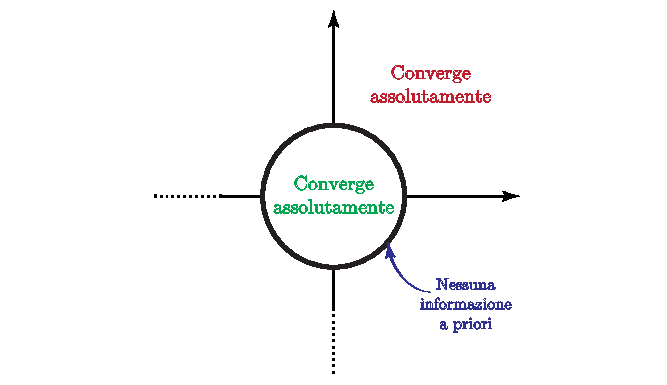
\includegraphics[trim=2.5cm 0.5cm 2.5cm 0cm, clip, scale=1]{images/discoconvergenza.pdf}
	\end{center}
\end{define}
Poiché sappiamo che la serie converge assolutamente per $\abs{z}<r$, lo studio del raggio di convergenza passa attraverso lo studio della serie assoluta associata $\displaystyle\sum_{n=0}^{+\infty}\abs{a_nz^n}$.\\
Per determinare il raggio di convergenza, possiamo ad esempio usare il \textbf{criterio di D’Alembert}\seeonlyindex{criterio!del rapporto}{criterio!di D’Alembert} o detto anche \textit{criterio del rapporto}\index{criterio!del rapporto}, che ci fornisce una condizione \textit{sufficiente} su come determinare il raggio di convergenza.
\begin{proposition}[Criterio di D’Alembert o del rapporto.]~{}\\
	Data la serie $\displaystyle\sum_{n=0}^{+\infty}a_nz^n$, se $a_n\neq 0$ definitivamente ed esiste il limite
	\begin{equation*}
		\lim_{n\to+\infty}\frac{\abs{a_{n+1}}}{\abs{a_{n}}}=L
	\end{equation*}
	allora
	\begin{enumerate}
		\item $L=0\implies R=+\infty$
		\item $L=+\infty\implies R=0$
		\item $0<L<+\infty\implies R=\frac{1}{L}$
	\end{enumerate}
\end{proposition}
Questa proposizione ha il vantaggio di essere operativamente utile, ma ovviamente solo se valgono le ipotesi: non è scontato che il limite del rapporto sia ben definito!\\
Un teorema più generale che vale \textit{per ogni serie} è il \textit{criterio della radice}\index{criterio!della radice} o altresì noto come \textbf{teorema di Cauchy-Hadamard}\seeonlyindex{criterio!del rapporto}{teorema!di Cauchy-Hadamard}.
\begin{theorema}[Teorema di Cauchy-Hadamard]~{}\\
	Sia data la serie di potenze
	\begin{equation*}
		\sum_{n=0}^{+\infty}a_nz^n
	\end{equation*}
	e sia
	\begin{equation}
		\lambda=\limsup_{n\to+\infty}\sqrt[n]{\abs{n}}
	\end{equation}
	Allora
	\begin{enumerate}
		\item Se $\lambda = 0$, la serie converge $\forall z\in\complexset$.
		\item Se $0<\lambda<+\infty$, la serie converge $R=\frac{1}{\lambda}$.
		\item Se $\lambda = +\infty$, la serie converge solo in $z=0$.
	\end{enumerate}

\end{theorema}
\begin{observe}
	I tre casi scritti esauriscono \textit{tutti} i casi possibili. Infatti, per la permanenza del segno del limsup\footnote{Nelle ‘‘Note aggiuntive'', a pagina XXX è possibile trovare la dimostrazione di questo risultato insieme ad altri relativi al limsup e liminf.} vale
	\begin{equation*}
		\sqrt[n]{\abs{a_n}}\geq 0,\ \forall n\geq 0\implies\limsup_{n\to+\infty}\sqrt[n]{\abs{a_n}}\geq 0
	\end{equation*}
\end{observe}
\begin{demonstration}\textsc{(del teorema di Cauchy-Hadamard.)}~{}\\
	Partiamo dal dimostrare il punto $2)$: dobbiamo provare che $R=\frac{1}{\lambda}$, ossia
	\begin{itemize}
		\item[a.] Se $\abs{z}<\nicefrac{1}{\lambda}$, allora $\displaystyle\sum_{n=0}^{+\infty}a_nz^n$ converge.
		\item[b.] Se $\abs{z}>\nicefrac{1}{\lambda}$, allora $\displaystyle\sum_{n=0}^{+\infty}a_nz^n$ \textit{non} converge.
	\end{itemize}
	La condizione (a.) infatti non basta per dimostrare che la convergenza è solo all'interno del cerchio. Proviamo ora le due tesi.
	\begin{itemize}
		\item[a.]	 Sia $z$ tale che $\abs{z}<\nicefrac{1}{\lambda}$. Se $z=0$ la serie banalmente converge perché ogni serie converge nel suo centro.\\
		Se $z\neq 0$, vale $\lambda<\nicefrac{1}{\abs{z}}$; consideriamo allora $\lambda'$ tale che $\lambda<\lambda'<\nicefrac{1}{\abs{z}}$: poiché $\lambda'>\lambda$, per la caratterizzazione del massimo limite si ha
		\begin{equation*}
			\textcolor{red}{\circled{\ast}}\quad\exists N\colon\forall n\geq N,\ \sqrt[n]{\abs{a_n}}<\lambda'
		\end{equation*}
		Proviamo che $\displaystyle\sum_{n=0}^{+\infty}a_nz^n$ converge assolutamente usando il criterio del confronto.
		\begin{equation*}
			\abs{a_nz^n}=\abs{a_n}\abs{z^n}=\abs{a_n}\abs{z}^n\substack{<}_{\textcolor{red}{\circled{\ast}}} \left(\lambda'\right)^n\abs{z}^n=\left(\lambda'\abs{z}\right)^n,\ \forall n\geq N
		\end{equation*}
		Questo è il termine $n$-esimo della serie geometrica $\displaystyle\sum_{n=0}^{+\infty}\left(\lambda'\abs{z}\right)^n$ di ragione $\lambda'\abs{z}$.\\
		Poiché $0<\lambda'\abs{z}<1$ per la scelta di $\lambda'$, la serie geometrica converge e quindi per il criterio del confronto converge anche la serie $\displaystyle\sum_{n=0}^{+\infty}\abs{a_nz^n}$ e dunque converge anche $\displaystyle\sum_{n=0}^{+\infty}a_nz^n$.
		\item[b.]	 Sia $z$ tale che $\abs{z}>\nicefrac{1}{\lambda}$. Per mostrare la non convergenza della serie proviamo che la condizione necessaria di convergenza non è soddisfatta, ovvero
		\begin{equation*}
			\lim_{n\to+\infty}a_nz^n\neq 0,\ \forall z\colon \abs{z}>\frac{1}{\lambda}
		\end{equation*}
		Per questo è sufficiente mostrare che
		\begin{equation*}
			\lim_{n\to+\infty}\abs{a_nz^n}\neq 0,\ \forall z\colon \abs{z}>\frac{1}{\lambda}
		\end{equation*}
		Notiamo che siamo passati da $\complexset$ a $\realset$ grazie alla norma, anche se in $\complexset$ ci trovavamo comunque in uno spazio metrico con la distanza indotta dal modulo.\\
		Poiché $z\neq 0$, vale $\lambda>\nicefrac{1}{\abs{z}}$.	Consideriamo allora $\lambda''$ tale che $\nicefrac{1}{\abs{z}}<\lambda''<\lambda$: poiché $\lambda''<\lambda$, per la caratterizzazione del massimo limite si ha
		\begin{equation*}
			\textcolor{blue}{\circled{\ast}}\quad\exists n_k\to+\infty\colon\sqrt[n_k]{\abs{a_{n_k}}}>\lambda''
		\end{equation*}
		Si ha, lungo la sottosuccessione:
		\begin{equation*}
			\abs{a_{n_k}z^{n_k}}=\abs{a_n}{z}^{n_k}\substack{>}_{\textcolor{blue}{\circled{\ast}}} \left(\lambda''\right)^{n_k}\abs{z}^{n_k}=\left(\substack{\lambda''\abs{z}>1}_{\text{ per la scelta di }\lambda''}\right)^{n_k}>1,\ \forall n_k
		\end{equation*}
		Poiché esiste una sottosuccessione che è sempre maggiore di $1$, deve esistere un valore limite della successione $\abs{a_nz^n}$ maggiore o uguale a $1$. Ma allora
		\begin{equation*}
			\limsup_{n\to+\infty}\abs{a_nz^n}\geq 1\implies\lim_{n\to+\infty}\abs{a_nz^n}\neq 0
		\end{equation*}
	\end{itemize}
	La dimostrazione del punto $1)$ è analoga alla prima parte della dimostrazione del punto $2)$. In questo caso, dobbiamo mostrare che la serie converge $\forall z\in\complexset$.\\ Se $z=0$, la serie banalmente converge, mentre se $z\neq 0$, si ha chiaramente che $0=\lambda<\nicefrac{1}{\abs{z}},\ \forall z\in\complexset\setminus\{0\}$. Consideriamo allora $\lambda'$ tale che $0<\lambda'<\nicefrac{1}{\abs{z}}$: poiché $\lambda'>0$, per la caratterizzazione del massimo limite si ha
	\begin{equation*}
		\textcolor{red}{\circled{\ast}}\quad\exists N\colon\forall n\geq N\ \sqrt[n]{\abs{a_n}}<\lambda'
	\end{equation*}
	Proviamo che $\displaystyle\sum_{n=0}^{+\infty}a_nz^n$ converge assolutamente usando il criterio del confronto.
	\begin{equation*}
		\abs{a_nz^n}=\abs{a_n}\abs{z^n}=\abs{a_n}\abs{z}^n\substack{<}_{\textcolor{red}{\circled{\ast}}} \left(\lambda'\right)^n\abs{z}^n=\left(\lambda'\abs{z}\right)^n,\ \forall n\geq N
	\end{equation*}
	Questo è il termine $n$-esimo della serie geometrica $\displaystyle\sum_{n=0}^{+\infty}\left(\lambda'\abs{z}\right)^n$ di ragione $\lambda'\abs{z}$.\\
	Poiché $0<\lambda'\abs{z}<1$ per la scelta di $\lambda'$, la serie geometrica converge e quindi per il criterio del confronto converge anche la serie $\displaystyle\sum_{n=0}^{+\infty}\abs{a_nz^n}$ e dunque converge anche $\displaystyle\sum_{n=0}^{+\infty}a_nz^n$. Poiché la scelta di $z$ è stata arbitraria, vale la tesi.\\
	La dimostrazione del punto $1)$ è analoga alla seconda parte della dimostrazione del punto $2)$. In questo caso, dobbiamo mostrare che la serie converge solo in $z=0$.\\ Se $z=0$, la serie banalmente converge. Per mostrare la non convergenza della serie proviamo che la condizione necessaria di convergenza non è soddisfatta, ovvero
	\begin{equation*}
		\lim_{n\to+\infty}a_nz^n\neq 0,\ \forall z\neq 0
	\end{equation*}
	Questo è equivalente a mostrare che
	\begin{equation*}
		\lim_{n\to+\infty}\abs{a_nz^n}\neq 0,\ \forall z\neq 0
	\end{equation*}
	Dato $z\neq 0$, consideriamo allora $\lambda''$ tale che $\nicefrac{1}{\abs{z}}<\lambda''<+\infty$: poiché $\lambda''<+\infty$, per la caratterizzazione del massimo limite si ha
	\begin{equation*}
		\textcolor{blue}{\circled{\ast}}\quad\exists n_k\to+\infty\colon\sqrt[n_k]{\abs{a_{n_k}}}>\lambda''
	\end{equation*}
	Si ha, lungo la sottosuccessione:
	\begin{equation*}
		\abs{a_{n_k}z^{n_k}}=\abs{a_n}{z}^{n_k}\substack{>}_{\textcolor{blue}{\circled{\ast}}}\left(\lambda''\right)^{n_k}\abs{z}^{n_k}=\left(\substack{\lambda''\abs{z}}_{>1\text{ per la scelta di }\lambda''}\right)^{n_k}>1,\ \forall n_k
	\end{equation*}
	Poiché esiste una sottosuccessione che è sempre maggiore di $1$, deve esistere un valore limite della successione $\abs{a_nz^n}$ maggiore o uguale a $1$. Ma allora
	\begin{equation*}
		\limsup_{n\to+\infty}\abs{a_nz^n}\geq 1\implies\lim_{n\to+\infty}\abs{a_nz^n}\neq 0
	\end{equation*}
	La scelta di $z$ è arbitraria, purché $z$ sia diverso da zero; per questo motivo vale la tesi.
\end{demonstration}
\section{Comportamento sul bordo}
Consideriamo la serie di potenze
\begin{equation*}
	\sum_{n=0}^{+\infty}a_nz^n,\quad a_n,\ z\in\complexset
\end{equation*}
con raggio di convergenza finito e non nullo.
I possibili comportamenti sul \textit{bordo} del cerchio di convergenza sono i seguenti:
\begin{enumerate}
	\item Convergenza in \textit{tutti i punti} del bordo del cerchio di convergenza
	\item \textit{Non} convergenza in \textit{nessun punto} del bordo del cerchio di convergenza
	\item Convergenza solo in \textit{alcuni punti} del bordo del cerchio di convergenza
\end{enumerate}
Mostriamo per ciascuno di essi un esempio.
\begin{example}\textsc{Caso 1.}~{}\\
	Consideriamo la serie
	\begin{equation*}
		\sum_{n=1}^{+\infty}\frac{z^n}{n^\alpha},\quad\alpha>1
	\end{equation*}
	Con la formula di D'Alembert vediamo che il raggio di convergenza è $R=1$. Infatti
	\begin{equation*}
		\lim_{n\to+\infty}\frac{\abs{a_{n+1}}}{\abs{a_{n}}}=\lim_{n\to+\infty}\frac{\left(n+1\right)^\alpha}{n^\alpha}=\lim_{n\to+\infty}\frac{n^\alpha\left(1+\frac{1}{n}\right)^\alpha}{n^\alpha}=\lim_{n\to+\infty}\left(1+\frac{1}{n}\right)^\alpha=1=\mathcal{l}\implies r=\frac{1}{\mathcal{l}}=1
	\end{equation*}
	Per ogni $z\in\complexset$ tale che $\abs{z}=1$ la serie converge (assolutamente):
	\begin{equation*}
		\sum_{n=1}^{+\infty}\abs{\frac{z^n}{n^\alpha}}=\sum_{n=1}^{+\infty}\frac{n}{n^\alpha}
	\end{equation*}
	La serie in modulo è la \textit{serie armonica generalizzata} che, per $\alpha>1$, converge; la serie semplice converge su tutti i punti del bordo.
\end{example}
\begin{example}\textsc{Caso 2.}~{}\\
	Consideriamo la \textit{serie geometrica}
	\begin{equation*}
		\sum_{n=1}^{+\infty}z^n
	\end{equation*}
	Poichè $a_n\equiv 1\ \forall n$, il criterio del rapporto ci fornisce come raggio di convergenza $R=1$.\\
	Per ogni $z\in\complexset$ tale che $\abs{z}=1$ la serie \textit{non} converge: possiamo osservare che presa la successione $c_n\in\complexset$, vale\footnote{Nelle ‘‘Note aggiuntive'', a pagina XXX è possibile trovare la dimostrazione di questo risultato.}
	\begin{equation*}
		\lim_{n\to+\infty}\abs{c_n}\neq 0\implies\lim_{n\to+\infty}c_n\neq 0
	\end{equation*}
	In questo caso:
	\begin{equation*}
		\lim_{n\to+\infty}\abs{z^n}=\lim_{n\to+\infty}1=1\neq 0\implies\lim_{n\to+\infty}z^n\neq 0
	\end{equation*}
	È evidente che la \textit{condizione necessaria} di convergenza \textit{non} è soddisfatta: la serie \textit{non} converge in nessun punto del bordo.
\end{example}
\begin{example}\textsc{Caso 3.}~{}\\
	Consideriamo la serie
	\begin{equation*}
		\sum_{n=1}^{+\infty}\frac{z^n}{n^\alpha},\quad0<\alpha<1
	\end{equation*}
	L'applicazione del criterio del confronto è esattamente analogo a quello visto nel caso  e il raggio di convergenza è pertanto $R=1$.\\
	Se $z=1$ la serie \textit{non} converge, dato che essa diventa una serie armonica generalizzata con $\alpha\leq1$:
	\begin{equation*}
		\sum_{n=1}^{+\infty}\frac{1}{n^\alpha}
	\end{equation*}
	Invece, per ogni $z\in\complexset$ tale che $\abs{z}=1$ e $z\neq 1$ la serie converge: infatti, possiamo applicare il \textit{criterio di Abel-Dirichlet}.
	\begin{equation*}
		\sum_{n=1}^{+\infty}\frac{z^n}{n^\alpha}=\sum_{n=1}^{+\infty}z^n\frac{1}{n^\alpha}=\sum_{n=1}^{+\infty}\alpha_n\beta_n
	\end{equation*}
	con $\alpha_n=z^n$ e $\beta_n=\nicefrac{1}{n^\alpha},\ n\geq 1$.
	\begin{enumerate}
		\item $\beta_n=\nicefrac{1}{n^\alpha}$ è una successione di elementi strettamente positivi, decrescenti e infinitesima per $n\to+\infty$.
		\item La successione delle \textit{somme parziali} di $\alpha_n=z^n$ è \textit{limitata}. Consideriamo
		\begin{equation*}
			\abs{\sum_{n=1}^{k}z^n}=\abs{\sum_{n=0}^{k}z^n-1}\squarequal
		\end{equation*}
		Poiché $\displaystyle\sum_{n=0}^{k}z^n$ è un serie geometrica parziale, sappiamo la sua somma parziale. Applicando poi una \textit{disuguaglianza triangolare}, troviamo una \textit{maggiorazione} della somma parziale di $\alpha_n$.
		\begin{equation*}
			\squarequal\abs{\frac{1-z^{k+1}}{1-z}-1}=\abs{\frac{z-z^{k+1}}{1-z}}\leq\frac{\abs{z}+\abs{-z^{k+1}}}{\abs{1-z}}\leq\frac{1+1}{\abs{1-z}}=\frac{2}{\abs{1-z}},\ \forall k\geq 1
		\end{equation*}
	\end{enumerate}
	Osserviamo che, nonostante la serie converga, essa non converge assolutamente: la serie in modulo è la serie armonica generalizzata con $\alpha\leq 1$, nota per essere divergente.
\end{example}
Anche se in generale non possiamo affermare a priori come converge sul bordo si può osservare che, in alcuni casi particolari, dalla convergenza in un punto del bordo si ottiene la convergenza sull'intero bordo. Vediamo alcuni risultati.
\begin{proposition}[Convergenza assoluta sul bordo se la serie di potenze converge assolutamente in un punto.]~{}\\
	Sia data la serie di potenze
	\begin{equation*}
		\sum_{n=1}^{+\infty}a_nz^n
	\end{equation*}
	Se la serie converge assolutamente in un punto della frontiera del cerchio di convergenza, allora converge assolutamente su tutta questa frontiera.
\end{proposition}
\begin{demonstration}
	Supponiamo che la serie converga assolutamente in $z_0$, dove $\abs{z_0}=R$ e prendiamo un qualunque $z$ tale che $\abs{z}=R$.
	Osserviamo che, presa la serie in modulo, si ha
	\begin{equation*}
		\sum_{n=1}^{+\infty}\abs{a_nz^n}=\sum_{n=1}^{+\infty}\abs{a_n}\abs{z^n}=\sum_{n=1}^{+\infty}\abs{a_n}\abs{z}^n=\sum_{n=1}^{+\infty}\abs{a_n}R^n=\sum_{n=1}^{+\infty}\abs{a_n}ì\abs{z_0}^n=\sum_{n=1}^{+\infty}\abs{a_nz_0^n}
	\end{equation*}
	che converge per ipotesi. Allora la serie di potenze converge assolutamente.
\end{demonstration}
\begin{corollary}[Convergenza sul bordo se la serie di potenze a coefficienti reali positivi converge in $z=R$.]~{}\\
	Sia data la serie di potenze
	\begin{equation*}
		\sum_{n=1}^{+\infty}a_nz^n
	\end{equation*}
	Se la serie ha coefficienti reali positivi e converge nel punto $z=R$, dove $R\in\left(0,+\infty\right)$ è il raggio di convergenza, allora converge in ogni punto della frontiera del cerchio di convergenza.
\end{corollary}
\begin{demonstration}
	Poiché $a_n$ e $R$ sono reali positivi, $a_n=\abs{a_n}$ e $R=\abs{R}$. Allora si ha
	\begin{equation*}
		\sum_{n=1}^{+\infty}a_nR^n=\sum_{n=1}^{+\infty}\abs{a_nR^n}
	\end{equation*}
	Quindi in questo caso la convergenza semplice della serie implica la convergenza assoluta. Poiché la serie converge assolutamente in un punto del bordo, segue dalla proposizione precedente la convergenza (assoluta) in tutti i punti del bordo.
\end{demonstration}
\section{Serie di potenze e convergenza uniforme}
\begin{theorema}[Converge uniforme delle serie di potenze.]~{}\\\label{convergenzasottoinsiemeH}
	Sia $\displaystyle\sum_{n=0}^{+\infty}a_nz^n$ una serie di potenze con raggio di convergenza $R\in\left(0,+\infty\right)$. Allora
	\begin{enumerate}
		\item La serie converge uniformemente su ogni insieme $H\subseteq\complexset$ tale che $\overline{H}\subsetneqq B_R\left(0\right)$, con $B_R\left(0\right)$ il disco aperto di convergenza, ovvero su qualsiasi insieme contenuto nel disco aperto tale che la sua chiusura non tocchi il bordo.
		\item Se la serie converge assolutamente in ogni $z\in\partial B_R\left(0\right)$ (il bordo del disco), allora converge uniformemente sul disco chiuso $\overline{B_R\left(0\right)}$.
	\end{enumerate}
\end{theorema}
\begin{demonstration} Per questa dimostrazione useremo il \textit{criterio di Weierstrass} enunciato nella sezione \ref{criteriodiweierstrass}, pag. \pageref{criteriodiweierstrass}.
	\begin{enumerate}
		\item Sia $H$ tale che $\overline{H}\subsetneqq B_R\left(0\right)$. Per il criterio di Weierstrass, per provare la convergenza uniforme su $H$ è sufficiente provare che esiste una successione $c_n$ tale che
		\begin{enumerate}
			\item $\abs{a_nz^n}\leq c_n,\ \forall z\in H$
			\item $\displaystyle\sum_{n=0}^{+\infty}c_n$ converge.
		\end{enumerate}
		\begin{minipage}{0.40\textwidth}
			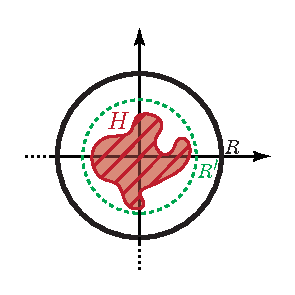
\includegraphics[trim=0cm 0cm 0cm 0cm, clip, scale=1]{images/discoconvergenzainsiemeH.pdf}
		\end{minipage}\hspace{-7mm}
		\begin{minipage}{0.55\textwidth}
			Poiché $H$ è solo \textit{strettamente contenuto} nel disco aperto di convergenza, $\exists R'<R$ tale che si abbia $\overline{H}\subseteq B_{R'}\left(0\right)$, ossia $\abs{z}\leq R',\ \forall z\in H$.\\
			Allora si ha, $\forall n\geq 0$ e $\forall z\in H$
			\begin{equation*}
				\abs{a_nz^n}=\abs{a_n}\abs{z}^n\leq \underbrace{\abs{a_n}\left(R'\right)^n}_{\text{$c_n$non dipende da }z}
			\end{equation*}
		\end{minipage}\\
		Inoltre, la serie $\displaystyle\sum_{n=0}^{+\infty}c_n=\sum_{n=0}^{+\infty}\abs{a_n}\left(R'\right)^n$ converge in quanto è la convergenza della serie di potenze per il punto $z=R'$, che è \textit{interno} al disco di convergenza $B_R\left(0\right)$. Applicando il criterio di Weierstrass otteniamo la tesi.
		\item Si ripete la dimostrazione sull'insieme $\overline{B_R\left(0\right)}$ con $R'=R$, considerando che la serie $\displaystyle\sum_{n=0}^{+\infty}\abs{a_n}R^n$ converge per ipotesi sulla convergenza sul bordo.
	\end{enumerate}
\end{demonstration}
\begin{example}\textsc{Serie geometrica.}\\
	Sulla \textit{serie geometrica} $\displaystyle\sum_{n=0}^{+\infty}z^n$ abbiamo già ricavato diverse informazioni: ha raggio di convergenza $R=1$ e \textit{non} c'è convergenza (assoluta) sul bordo, inoltre ne conosciamo la somma. Studiamo ora la convergenza uniforme.
	\begin{itemize}
		\item Converge uniformemente su ogni insieme $H$ tale che $\overline{H}\subsetneqq B_1\left(0\right)$ per il teorema precedente.
		\item Non avendo alcuna convergenza sul bordo, a priori non possiamo dare risultati generali sulla convergenza uniforme sulla base del teorema visto. Tuttavia, possiamo mostrare direttamente - grazie al fatto che la somma parziale e limite della serie geometrica è nota\footnote{Nelle ‘‘Note aggiuntive'', a pagina XXX è possibile trovare maggiori dettagli sulla somma (parziale) della serie geometrica e come ricavarla.} -  che la serie non converge uniformemente sul disco aperto $B_1\left(0\right)$. Infatti
		\begin{align*}
			\sup_{z\in B_1\left(0\right)}\abs{S_n\left(z\right)-S\left(z\right)}&=\sup_{z\in B_1\left(0\right)}\abs{\frac{1-z^{n+1}}{1-z}-\frac{1}{1-z}}=\sup_{z\in B_1\left(0\right)}\abs{\frac{-z^{n+1}}{1-z}}=\\
			&=\sup_{z\in B_1\left(0\right)}\frac{\abs{z}^{n+1}}{\abs{1-z}}=+\infty,\ \forall n\geq 0
		\end{align*}
		da cui
		\begin{equation*}
			\lim_{n\to+\infty}\left(\sup_{z\in B_1\left(0\right)}\abs{S_n\left(z\right)-S\left(z\right)}\right)=+\infty\neq 0
		\end{equation*}
	\end{itemize}
\end{example}
\section{Proprietà di regolarità della somma di una serie di potenze}
Sia $\displaystyle\sum_{n=0}^{+\infty}a_nz^n$ una serie di potenze con $R>0$ il raggio di convergenza. Studiamo le proprietà di continuità e derivabilità della \textbf{funzione somma}\index{funzione!somma}
\begin{equation}
	\funztot{f}{B_R\left(0\right)\subseteq\complexset}{\complexset}{z}{\displaystyle\sum_{n=0}^{+\infty}a_nz^n}
\end{equation}
\subsection{Continuità}
\begin{proposition}[Proprietà di continuità per la somma di una serie di potenze, caso generale.]~{}\\
	La funzione $f$ è continua su $B_R\left(0\right)$.
\end{proposition}
\begin{attention}
	La convergenza della serie di potenze su $B_R\left(0\right)$ \textit{non} è in generale uniforme, ma sappiamo al più che converge uniformemente su $H$ tale che $\overline{H}\subsetneqq B_R\left(0\right)$, quindi dobbiamo tenere conto di questo fattore nelle dimostrazioni che faremo.
\end{attention}
\begin{demonstration}
	Dobbiamo provare che $f\in\mathcal{C}\left(B_R\left(0\right)\right)$, cioè $f$ continua in $z_0,\ \forall z_0\in B_R\left(0\right)$. Sfrutto il fatto che la continuità è una proprietà locale, quindi fisso un punto e studio la continuità nel punto.\\	\vspace{3mm}
	\begin{minipage}{0.44\textwidth}
		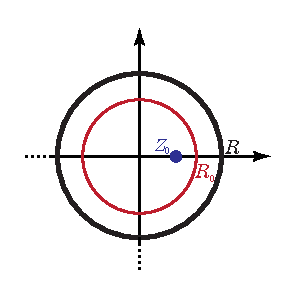
\includegraphics[trim=0cm 0cm 0cm 0cm, clip, scale=1.1]{images/discoconvergenzacontinuitaf.pdf}
	\end{minipage}\hspace{-9mm}
	\begin{minipage}{0.60\textwidth}
		Sia $z_0\in B_R\left(0\right)$ fissato. Per proprietà della metrica, allora $\exists R_0 < R$ tale che $z_0\in B_{R_0}\left(0\right)$. Su $B_{R_0}\left(0\right)$ si ha continuità uniforme e dunque, posto
		\begin{equation*}
			S_n\left(z\right)=\sum_{k=0}^{n}a_kz^k
		\end{equation*}
		si ha
		\begin{enumerate}
			\item $S_n$ continua su $B_{R_0}\left(0\right)$ perché è un polinomio.
			\item $S_n$ converge uniformemente a $f$ su $B_R\left(0\right)$.
		\end{enumerate}
	\end{minipage}\\
	Per il teorema di continuità della funzione limite, $f$ è continua in $B_{R_0}\left(0\right)$ e dunque in $z_0$. 
\end{demonstration}
%FINO A QUI
Questo risultato ci permette di parlare della convergenza sul disco aperto, ma se c'è qualche tipo di convergenza sul bordo, e quindi $f$ è definita anche su di esso, si può estendere la continuità di $f$ fino a tale frontiera? Studiamo due casi.
\begin{corollary}[Proprietà di continuità per la somma di una serie di potenze, caso sul bordo con convergenza assoluta.]~{}\\
	Sia data la serie di potenze $\displaystyle\sum_{n=0}^{+\infty}a_nz^n$ con raggio di convergenza $R>0$. Se la serie converge (assolutamente) su $\partial B_R\left(0\right)$ allora la serie è continua su $\overline{B_R\left(0\right)}$.
\end{corollary}
\begin{demonstration}
	Segue immediatamente ricordando che dalle ipotesi di convergenza assoluta sul bordo, sulla base del teorema \ref{convergenzasottoinsiemeH}, pag. \pageref{convergenzasottoinsiemeH}, vale la convergenza uniforme su $\overline{B_R\left(0\right)}$.
\end{demonstration}
Se invece supponiamo che la serie converga in un punto\footnote{Nel caso di più punti di convergenza $z_0,\ z_1,\ \ldots$, la funzione somma $f$ sarà definita su $B_R\left(0\right)\cup\left\{z_0\right\}\cup\left\{z_1\right\}\cup\ldots$. Qui riportiamo per semplicità il caso di un solo punto, ma i risultati successivi sono opportunamente generalizzabili con più punti di convergenza sul bordo.} $z_0$, cioè $\displaystyle\sum_{n=0}^{+\infty}a_nz_0^n$ converge, possiamo definire la \textbf{funzione somma}\index{funzione!somma} come
\begin{equation}
	\funztot{f}{B_R\left(0\right)\cup\left\{z_0\right\}\subseteq\complexset}{\complexset}{z}{\displaystyle\sum_{n=0}^{+\infty}a_nz^n}
\end{equation}
La convergenza uniforme di $f$ anche sui punti di convergenza $z_0$ sul bordo ci viene garantita dal \textbf{teorema di Abel}\index{teorema!di Abel}.
\begin{theorema}[Teorema di Abel.]~{}\\
	Sia dato la serie di potenze la serie di potenze $\displaystyle\sum_{n=0}^{+\infty}a_nz^n$ con raggio di convergenza $R>0$. Se $\exists z_0=Re^{i\theta_0}$ tale che $\displaystyle\sum_{n=0}^{+\infty}a_nz_0^n$ converge, allora\\
	\begin{minipage}{0.39\textwidth}
		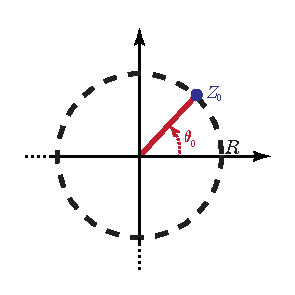
\includegraphics[trim=0cm 0cm 0cm 0cm, clip, scale=1]{images/discoconvergenzaabel.pdf}
	\end{minipage}\hspace{-12mm}
	\begin{minipage}{0.65\textwidth}
		\begin{enumerate}
			\item la serie converge uniformemente sul \textit{segmento}
			\begin{equation}
				\Sigma_0=\left\{z\in\complexset\mid z=re^{i\theta_0},\ r\in\left[0,R\right]\right\}
			\end{equation}
			\item La restrizione di $f$ a $\Sigma_0$ è \textit{continua} su $z_0$, ossia
			\begin{equation}
				\lim_{r\to R}f\left(re^{i\theta_0}\right)=f\left(z_0\right)=\sum_{n=0}^{+\infty}a_nz_0^n
			\end{equation}
		\end{enumerate}
	\end{minipage}
\end{theorema}
\subsection{Derivabilità}
Abbiamo definito la funzione somma dal disco aperto $B_R\left(0\right)$ in campo complesso a $\complexset$, ma al momento non conosciamo cosa vuol dire derivabilità di una funzione $\funz{f}{\complexset}{\complexset}$. Per il momento, limitiamoci al caso reale, cioè consideriamo una serie di potenze
\begin{equation*}
	\sum_{n=0}^{+\infty}a_nx^n,\ x\in\realset,\ a_n\in\realset
\end{equation*}
con raggio di convergenza $R>0$. In questo caso il cerchio di convergenza è un intervallo $\left(-R,R\right)$, con estremi eventualmente inclusi. La funzione somma risulta allora la funzione
\begin{equation}
	\funztot{f}{\left(-R,R\right)}{\realset}{x}{\sum_{n=0}^{+\infty}a_nx^n}
\end{equation}
\begin{theorema}[Derivabilità della somma di una serie di potenze.]~{}\\
	Sia data
	\begin{equation*}
		f\left(x\right)=\sum_{n=0}^{+\infty}a_nx^n,\ \forall x\in\left(-R,R\right),\ a_n\in\realset
	\end{equation*}
con $R>0$ il raggio di convergenza. Allora
\begin{enumerate}
	\item $f$ è derivabile su $\left(-R,R\right)$
	\item La derivata di $f$ è
	\begin{equation}
		f'\left(x\right)=\sum_{n=1}^{+\infty}na_nx^{n-1},\ \forall x\in\left(-R,R\right)
	\end{equation}
\end{enumerate}
\end{theorema}
Per dimostrare questo teorema useremo il teorema di derivibilità per serie di funzioni (teorema \ref{derivabilitatermineatermine}, pag. \pageref{derivabilitatermineatermine}, capitolo \refChapter{seriefunzioni}): poiché le ipotesi $1)$ e $2)$ sono banalmente verificate, dobbiamo contrarci sull'ipotesi $3)$, ovvero abbiamo bisogno di informazioni sulla convergenza uniforme della serie delle derivate $\displaystyle\sum_{n=1}^{+\infty}na_nx^{n-1}$; poiché la serie delle derivate è ancora una serie di potenze, allora ci basta studiare il raggio di convergenza.
% TO DO: nelle Note extra a pagina XXX inserire il prodotto del lim sup
\begin{lemming}[Convergenza della serie di derivate della serie di potenze.]~{}\\
	Sia data la serie di potenze $\displaystyle\sum_{n=0}^{+\infty}a_nx^n$ e sia $R>0$ il suo raggio di convergenza. Allora la serie di potenze $\displaystyle\sum_{n=1}^{+\infty}na_nx^{n-1}$ ha raggio di convergenza $R$.
\end{lemming}
\begin{demonstration}
	Riscriviamo la serie delle derivate, operando un cambio di indici ponendo $n=k+1$
	\begin{equation*}
		\sum_{n=1}^{+\infty}na_nx^{n-1}=\sum_{k=0}^{+\infty}\underbrace{\left(k+1\right)a_{k+1}}_{=b_k}x^k=\sum_{k=0}^{+\infty}b_ka_k
	\end{equation*}
	Sia $R'$ il suo raggio di convergenza. Per il teorema di Cauchy-Hadamard si ha
	\begin{equation*}
		\frac{1}{R'}=\limsup_{n\to+\infty}\abs{b_n}^{\nicefrac{1}{n}}=\limsup_{n\to+\infty}\abs{\left(n+1\right)a_{n+1}}^{\nicefrac{1}{n}}=\limsup_{n\to+\infty}\underbrace{\left(n+1\right)^{\nicefrac{1}{n}}}_{=\alpha_n}\underbrace{\abs{a_{n+1}}^{\nicefrac{1}{n}}}_{=\beta_n}=\limsup_{n\to+\infty}\alpha_n\beta_n\squarequal
	\end{equation*}
Osserviamo che
\begin{equation*}
	\lim_{n\to+\infty}\alpha_n=\lim_{n\to+\infty}\left(n+1\right)^{\nicefrac{1}{n}}=\lim_{n\to+\infty}e^{\frac{1}{n}\log\left(n+1\right)}=\lim_{n\to+\infty}e^{\frac{\log\left(n+1\right)}{n}}
\end{equation*}
Poichè $\frac{\log\left(n+1\right)}{n}\to 0$ per $n\to+\infty$ per confronto della crescita degli infiniti, $\displaystyle\lim_{n\to+\infty}\alpha_n=e^0=1$, dunque $\alpha_n$ ammette limite e dunque coincide col suo $\limsup$. Allora, per proprietà\footnote{Nelle ‘‘Note aggiuntive'', a pagina XXX è possibile trovare la dimostrazione di questo risultato insieme ad altri relativi al limsup e liminf.} del $\limsup$:
\begin{equation*}
	\squarequal\lim_{n\to+\infty}\alpha_n\limsup_{n\to+\infty}\beta_n=\limsup_{n\to+\infty}\abs{a_{n+1}}^{\nicefrac{1}{n}}=\limsup_{n\to+\infty}\left(\abs{a_{n+1}}^{\nicefrac{1}{n+1}}\right)^{\nicefrac{n+1}{n}}\squarequal
\end{equation*}
Poichè $\nicefrac{n+1}{n}\to 1$ per $n\to+\infty$, possiamo applicare Cauchy-Hadamar sulla serie di potenze $\displaystyle\sum_{n=0}^{+\infty}a_nx^n$ con raggio di convergenza $R>0$: poiché
\begin{equation*}
	\frac{1}{R}=\limsup_{n\to+\infty}\abs{a_n}^{\nicefrac{1}{n}}=\limsup_{n\to+\infty}\abs{a_{n+1}}^{\nicefrac{1}{n+1}}
\end{equation*}
allora abbiamo mostrato che
\begin{equation*}
	\frac{1}{R'}=\ldots=\limsup_{n\to+\infty}\left(\abs{a_{n+1}}^{\nicefrac{1}{n+1}}\right)^{\nicefrac{n+1}{n}}=\frac{1}{R}
\end{equation*}
cioè $R'=R$.
\end{demonstration}
Grazie a questo lemma, possiamo finalmente dimostrare il teorema lasciato in sospeso all'inizio della sezione.
\begin{demonstration}\textsc{(del Teorema di derivabilità della somma di una serie di potenze.)}\\
	Fissiamo $\overline{x}\in\left(-R,R\right)$ arbitrario e sia $\left(a,b\right)$ tale che
	\begin{itemize}
		\item $\overline{x}\in\left(a,b\right)$.
		\item $\left[a,b\right]\subsetneqq\left(-R,R\right)$
	\end{itemize}
Applichiamo ora il teorema di derivabilità termine a termine della serie di funzioni su $\left(a,b\right)$ sulla serie di potenze $\displaystyle\sum_{n=0}^{+\infty}a_nx^n$; vediamo che le ipotesi sono verificate:
\begin{itemize}
	\item $f_n\left(x\right)=a_nx^n$ derivabile in $\left(a,b\right),\ \forall n\geq 1$.
	\item $\displaystyle\sum_{n=0}^{+\infty}f_n\left(x\right)$ converge $\forall x\in\left(a,b\right)$
	\item $\displaystyle\sum_{n=1}^{+\infty}f'_n\left(x\right)=\sum_{n=1}^{+\infty}na_nx^{n-1}$ converge uniformemente su $\left(a,b\right)$ per la scelta di $\left(a,b\right)$, sulla base del lemma precedentemente dimostrato.
\end{itemize}
Per il teorema di derivabilità termine a termine $f$ è derivabile in $\left(a,b\right)$ e dunque anche in $\overline{x}$, con derivata in tal punto
\begin{equation*}
	f'\left(\overline{x}\right)=\sum_{n=1}^{+\infty}na_nx^{n-1}
\end{equation*}
Per l'arbitrarietà di $\overline{x}$, questi risultati valgono $\forall x\in\left(-R,R\right)$ e dunque segue la tesi.
\end{demonstration}
\section{Funzioni analitiche e serie di Taylor}
La tesi $2)$ appena dimostrata ci dice che la derivata $f'$ è una somma di serie di potenze con stesso raggio di convergenza $R$ di $f$. Possiamo riapplicare il teorema alla funzione $f'$:
\begin{itemize}
	\item $f'$ è derivabile in $\left(-R,R\right)$.
	\item $\displaystyle f''\left(x\right)=\sum_{n=2}^{+\infty}n\left(n-1\right)a_nx^{n-2},\ \forall x\in\left(-R,R\right)$.
\end{itemize}
Ma anche $f''$ è una serie di potenze con raggio $R$: possiamo riapplicare il teorema su $f''$ e ammettere l'esistenza di $f'''$ come serie di potenze. Iterando il ragionamento, si trova che esiste $f^{\left(k\right)}\left(x\right),\ \forall x\in\left(-R,R\right),\ \forall k\geq 0$ e vale
\begin{equation}
	f^{\left(k\right)}\left(x\right)=\sum_{n=k}^{+\infty}n\left(n-1\right)\ldots\left(n-k+1\right)a_nx^{n-k}=\sum_{n=k}^{+\infty}\frac{n!}{\left(n-k\right)!}a_nx^{n-k},\ \forall x\in\left(-R,R\right)
\end{equation}
Esplicitiamo il primo termine di $f^{\left(k\right)}\left(x\right)$:
\begin{align*}
	f^{\left(k\right)}\left(x\right)&=k\left(k-1\right)\ldots\left(k-k+1\right)a_kx^0+\sum_{n=k+1}^{+\infty}n\left(n-1\right)\ldots\left(n-k+1\right)a_nx^{n-k}=\\
	&=k!a_k+\sum_{n=k+1}^{+\infty}n\left(n-1\right)\ldots\left(n-k+1\right)a_nx^{n-k}
\end{align*}
In $x=0$ otteniamo
\begin{equation*}
	f^{\left(k\right)}\left(0\right)=k!a_k+0=k!a_k
\end{equation*}
Da cui otteniamo una espressione del termine $a_k$ in funzione della derivata $k$-esima, supponendo che esiste tale derivata:
\begin{equation}
	a_k=\frac{f^{\left(k\right)}}{k!},\ \forall k\geq 0
\end{equation}
Riscriviamo questi risultati in un unico teorema.
\begin{theorema}[Analiticità della somma di una serie di potenze.]~{}\\
	Sia data la serie di potenze
	\begin{equation*}
		\sum_{n=0}^{+\infty}a_nx^n,\ a_n\in\realset, x\in\realset
	\end{equation*}
con raggio di convergenza $R>0$ e sia $f$ la sua somma. Allora
\begin{enumerate}
	\item $f\in\mathcal{C}^{\infty}\left(\left(-R,R\right)\right)$.
	\item La derivata $k$-esima è nella forma
	\begin{equation}
		f^{\left(k\right)}\left(x\right)=\sum_{n=k}^{+\infty}n\left(n-1\right)\ldots\left(n-k+1\right)a_nx^{n-k}=\sum_{n=k}^{+\infty}\frac{n!}{\left(n-k\right)!}a_nx^{n-k},\ \forall x\in\left(-R,R\right)
	\end{equation}
	\item Il coefficiente $a_k$ si può scrivere come
	\begin{equation}
		a_k=\frac{f^{\left(k\right)}}{k!},\ \forall k\geq 0
	\end{equation}
	\item $f$ è \textit{analitica} in $0$, ossia si può scrivere come una \textbf{serie di Taylor di }$f$\textbf{centrata in }$x=0$\index{serie!di Taylor}
	\begin{equation}
		f\left(x\right)=\sum_{k=0}^{+\infty}\frac{f^{\left(k\right)}}{k!}x^k,\ \forall x\in\left(-R,R\right)
	\end{equation}
\end{enumerate}
\end{theorema}
Diamo una definizione formale del termine ‘‘funzione analitica'' che abbiamo appena usato nel teorema.
\begin{define}[Funzione analitica.]~{}\\
	Sia $\funz{f}{U\subseteq \realset}{\realset}$ tale che $f\in\mathcal{C}^{\infty}\left(U\right)$.
	\begin{enumerate}
		\item Dato $x_0\in\ U$, $f$ si dice \textbf{analitica}\index{analitica} in $x_0$ se $\exists r_0>0$ tale che
		\begin{equation*}
			f\left(x\right)=\sum_{k=0}^{+\infty}\frac{f^{\left(k\right)}\left(x_0\right)}{k!}\left(x-x_0\right)^k,\ \forall x\in\left(x_0-r_0,x_0+r_0\right)\subseteq U
		\end{equation*}
		\item f si dice \textbf{analitica in }$U$ se è analitica in ogni punto $x_0\in U$. In questo caso si scrive $f\in\mathcal{A}\left(U\right)$.
	\end{enumerate}
\end{define}
Il problema della \textit{ricostruzione} di una funzione come somma della sua serie di Taylor, introdotto nello studio della lunghezza dell'ellisse nel \refChapter{ellipseintroduction}, si può anche formulare come
\begin{center}
	‘‘Ogni funzione $f\in\mathcal{C}^{\infty}\left(U\right)$ è anche analitica su $U$?''
\end{center}
ossia
\begin{equation*}
	f\in\mathcal{C}^{\infty}\left(U\right)\stackrel{?}{\implies}f\in\mathcal{A}\left(U\right)
\end{equation*}
In generale la risposta è \textbf{no}, come possiamo vedere nell'esempio successivo.
\begin{example}
	Consideriamo la funzione
	\begin{equation*}
		f\left(x\right)=
		\begin{cases}
			\begin{array}{ll}
				e^{-\frac{1}{x^2}}&\text{se }x\neq 0\\
				0&\text{se }x=0
			\end{array}
		\end{cases}
	\end{equation*}
$f$ è certamente di classe $\mathcal{A}^{\infty}\left(\realset\setminus\left\{0\right\}\right)$; si verifica che esiste $f^{\left(k\right)}=0,\ \forall k\geq 0$ e che $f^{\left(k\right)}\in\mathcal{C}\left(\realset\right),\ \forall k\geq 0$, dunque $f\in\mathcal{C}\left(\realset\right)$:\\
Tuttavia, $f\notin\mathcal{A}\left(\realset\right)$. Infatti, la serie di Taylor centrata in $x_0=0$ è
\begin{equation*}
	\sum_{k=0}^{+\infty}\frac{f^{\left(k\right)}\left(0\right)}{k!}x^k=\sum_{k=0}^{+\infty}\frac{0}{k!}x^k\equiv 0
\end{equation*}
che converge ma \textit{non} a $f$, ossia $f\left(x\right)\neq 	\sum_{k=0}^{+\infty}\frac{f^{\left(k\right)}\left(0\right)}{k!}x^k,\ \forall x\neq 0$.
\end{example}
% TO DO: controesempio su moodle
Bisogna quindi capire sotto quali ipotesi ulteriori una funzione di classe $\mathcal{C}^{\infty}$ è anche analitica; cerchiamo a tal scopo una condizione \textit{sufficiente}.\\
Riprendiamo il problema come era stato posto originalmente; approssimiamo $f$ con il \textit{polinomio} di Taylor, tenendo conto del \textit{resto} $R_n\left(x\right)$:
\begin{equation*}
	f\left(x\right)=\sum_{k=0}^{n}\frac{f^{\left(k\right)}\left(x_0\right)}{k!}\left(x-x_0\right)^k+R_n\left(x\right)
\end{equation*}
Per passare da questa approssimazione alla riscrittura di $f$ come \textit{serie} di Taylor è necessario ridurre il resto dell'approssimazione a zero al crescere dei termini del polinomio, ossia
\begin{equation*}
	\lim_{n\to+\infty}R_n\left(x\right)=0
\end{equation*}
Ricordiamo l'espressione del resto in \textit{forma di Lagrange}:
\begin{equation*}
	\exists \xi=\xi_{x,n}\colon R_n\left(x\right)=\frac{f^{\left(n+1\right)}\left(\xi\right)}{\left(n+1\right)!}\left(x-x_0\right)^{n+1}
\end{equation*}
La condizione sufficiente che andremo ora a definire necessita di avere una informazione sulle derivate $f^{\left(n\right)}$ per $n$ \textit{sufficientemente grande}.
\begin{theorema}[Condizione sufficiente di analiticità.]~{}\\\label{condizionesufficienteanaliticita}
	Sia $\funz{f}{U\subseteq\realset}{\realset}$, $f\in\mathcal{C}^{\infty}\left(U\right)$ e sia $x_0\in U$. Se $\exists r_0>0,\ \exists M>0,\ \exists n_0>0$ tale che
	\begin{equation}
		\abs{f^{\left(n\right)}\left(x\right)}\leq\frac{Mn!}{r_0^n},\ \forall x\in\left(x_0-r_0,x_0+r_0\right),\ \forall n\geq n_0
	\end{equation}
	allora $f$ è \textit{analitica} in $x_0$ e vale
	\begin{equation*}
		f\left(x\right)=\sum_{k=0}^{+\infty}\frac{f^{\left(k\right)}\left(x_0\right)}{k!}\left(x-x_0\right)^k,\ \forall x\in\left(x_0-r_0,x_0+r_0\right)
	\end{equation*}
\end{theorema}
\begin{demonstration}
	Sia $x\in\left(x_0-r_0,x_0+r_0\right)$ fissato. Dobbiamo provare che
	\begin{equation*}
		\lim_{n\to+\infty}R_n\left(x\right)=\lim_{n\to+\infty}\frac{f^{\left(n+1\right)}\left(\xi\right)}{\left(n+1\right)!}\left(x-x_0\right)^{n+1}=0
	\end{equation*}
dove $\xi$ è ottenuto applicando la formula di Taylor con il resto in \textit{formula di Lagrange}. Poiché $\xi\in\left(x_0-r_0,x_0+r_0\right)$, per l'ipotesi di partenza si può stimare $f^{\left(n+1\right)}\left(\xi\right)$:
\begin{align*}
	0\leq \abs{\frac{f^{\left(n+1\right)}\left(\xi\right)}{\left(n+1\right)!}\left(x-x_0\right)^{n+1}}&=\frac{\abs{f^{\left(n+1\right)}\left(\xi\right)}}{\left(n+1\right)!}\abs{x-x_0}^{n+1}\stackrel{\leq}{\forall n\geq n_0}\frac{\frac{M\Ccancel[red]{\left(n+1\right)!}}{r_0^{n+1}}}{\Ccancel[red]{\left(n+1\right)!}}\abs{x-x_0}^{n+1}=\\
	&=M\frac{\abs{x-x_0}^{n+1}}{r_0^{n+1}}=M\left(\frac{\abs{x-x_0}}{r_0}\right)^{n+1}
\end{align*}
Abbiamo quindi ottenuto
\begin{equation*}
	0\leq \abs{R_n\left(x\right)}\leq M\left(\frac{\abs{x-x_0}}{r_0}\right)^{n+1},\ \forall n\geq n_0
\end{equation*}
Poiché $\left(\frac{\abs{x-x_0}}{r_0}\right)^{n+1}$ è una successione geometrica di ragione $\frac{\abs{x-x_0}}{r_0}\in\left(0,1\right)$, essa tende a $0$ per $n\to+\infty$: per il teorema del confronto abbiamo $\displaystyle\lim_{n\to+\infty}R_n\left(x\right)=0$.
\end{demonstration}
\begin{observe}\label{condizionesufficientederivatelimitate}
	Questa condizione sufficiente si verifica anche se $\exists M>0, \exists r_0>0$ tale per cui
	\begin{equation*}
		\abs{f^{\left(n\right)}\left(x\right)}\leq M,\ \forall x\in\left(x_0-r_0,x_0+r_0\right),\ \forall n\geq 0
	\end{equation*}
Infatti, $\forall r_0>0$, per confronto di crescita si ha
\begin{equation*}
	\lim_{n\to+\infty}\frac{n!}{r_0^n}=+\infty
\end{equation*}
Dunque esiste sempre $n_0$ tale che $\forall n\geq n_0$ si ha $\frac{n!}{r_0^n}>1$. Segue allora
\begin{equation*}
	\abs{f^{\left(n\right)}\left(x\right)}\leq M<M\frac{n!}{r_0^n},\ \forall x\in\left(x_0-r_0, x_0+r_0\right),\ \forall n\geq n_0
\end{equation*}
\end{observe}
\section{Esempi di funzioni analitiche}
\begin{theorema}[Analiticità di {$e^x$}, {$\cos x$}, {$\sin x$}, {$\left(1+x\right)^\alpha$}.]~{}\\
	Le funzioni $e^x$, $\cos x$, $\sin x$, $\left(1+x\right)^\alpha$ con $\alpha\in\realset$ sono analitiche in $x_0=0$ e vale
	\begin{align}
		e^x&=\sum_{k=0}^{+\infty}\frac{1}{k!}x^k,\ \forall x\in\realset\\
		\sin x&=\sum_{k=0}^{+\infty}\frac{\left(-1\right)^k}{\left(2k\right)!}x^{2k},\ \forall x\in\realset\\
		\cos x&=\sum_{k=0}^{+\infty}\frac{\left(-1\right)^k}{\left(2k+1\right)!}x^{2k+1},\ \forall x\in\realset\\
		\left(1+x\right)^\alpha&=\sum_{k=0}^{+\infty}\binom{\alpha}{k}x^k,\ \forall x\in\left(-1,1\right),\ \forall \alpha\in\realset
	\end{align}
\end{theorema}
\begin{attention}
	L'ultima formula vale solo per $x\in\left(-1,1\right)$, indipendentemente dal dominio di $\left(1+x\right)^\alpha$. Ad esempio, se $\alpha=\frac{1}{3}$, $\left(1+x\right)^\alpha=\sqrt[3]{1+x}$ è definita su tutto $\realset$, però si può scrivere somma della sua serie di Taylor solo in $\left(-1,1\right)$; in altre parole, l'analiticità è una proprietà \textit{locale}.
\end{attention}
Le prime tre formule si dimostrano usando la condizione sufficiente precedentemente dimostrata. Per quanto riguarda la quarta formula, \textit{non} si riesce a verificare la validità di tale condizione, ma con un altro ragionamento si trova comunque l'analiticità. Questo mostra che la condizione scritta sopra è \textit{solo} sufficiente, ma \textit{non} necessaria per l'analiticità.
\begin{demonstration}~{}
	\begin{itemize}
		\item $e^x$, $\sin x$, $\cos x$. È noto che
		\begin{equation*}
			\sum_{k=0}^{n}\frac{1}{k!}x^k\quad\sum_{k=0}^{n}\frac{\left(-1\right)^k}{\left(2k\right)!}x^{2k}\quad\sum_{k=0}^{n}\frac{\left(-1\right)^k}{\left(2k+1\right)!}x^{2k+1}
		\end{equation*}
		sono i polinomi di Taylor di $e^x,\ \cos x$ e $\sin x$ centrati in $x_0=0$. Per $n\to+\infty$ si ottengono le serie di Taylor
		\begin{equation*}
			\sum_{k=0}^{+\infty}\frac{1}{k!}x^k\quad\sum_{k=0}^{+\infty}\frac{\left(-1\right)^k}{\left(2k\right)!}x^{2k}\quad\sum_{k=0}^{+\infty}\frac{\left(-1\right)^k}{\left(2k+1\right)!}x^{2k+1}
		\end{equation*}
	Proviamo ora che valgono le uguaglianze scritte. Per dimostrare che valgono su tutto $\realset$ è sufficiente dimostrate che valgono su un intervallo del tipo $\left(-r_0, r_0\right)$ con $r_0>0$ arbitrario.\\
	Sia allora $r_0>0$ fissato arbitrariamente e sia $x\in\left(-r_0, r_0\right)$. Proviamo che è vera la condizione a pag. \pageref{condizionesufficientederivatelimitate}, che sappiamo implicare la condizione sufficiente a pag. \pageref{condizionesufficienteanaliticita}. Vediamo i tre casi:
	\begin{itemize}
		\item $e^x$. La derivata di $f\left(x\right)=e^x$ è $f^{\left(n\right)}\left(x\right)=e^x$, quindi si ha
		\begin{equation*}
			\abs{f^{\left(n\right)}\left(x\right)}=e^x\leq e^{r_0}= M,\ \forall x\in\left(-r_0,r_0\right),\ \forall n\geq 0
		\end{equation*}
		\item $\cos x$, $\sin x$. Poiché le derivate di seno e coseno sono ciclicamente seno e coseno con opportuni segni, la derivata $n$-esima di $\cos x$ e $\sin x$ in modulo è sempre limitata da 1.
		\begin{equation*}
			\abs{f^{\left(n\right)}\left(x\right)}\leq 1 = M,\ \forall x\in\left(-r_0,r_0\right),\ \forall n\geq 0
		\end{equation*}
	\end{itemize}
	Poiché la condizione è verificata su $\left(-r_0,r_0\right)$ e vale l'analiticità su tale intervallo, per l'arbitrarietà di $r_0$ l'analiticità si verifica su tutto $\realset$.
	\item $\left(1+x\right)^\alpha$. Mostriamo innanzitutto che la serie di potenze $\displaystyle\sum_{n=0}^{+\infty}\binom{\alpha}{k}x^k$ converge $\forall x\in\left(-1,1\right)$, usando il criterio del rapporto:
	\begin{align*}
		R&=\lim_{n\to+\infty}\frac{\abs{a_n}}{\abs{a_{n+1}}}=\lim_{n\to+\infty}\frac{\abs{\alpha\left(\alpha-1\right)\ldots\left(\alpha-n+1\right)}}{n!}\frac{\left(n+1\right)!}{|\alpha\left(\alpha-1\right)\underbrace{\left(\alpha-\left(n+1\right)+1\right)}_{\alpha-n}|}=\\
		&=\lim_{n\to+\infty}\frac{\abs{n+1}}{\abs{\alpha-n}}=\lim_{n\to+\infty}\frac{n+1}{n-\alpha}=1
	\end{align*}
	Adesso definiamo la funzione somma
	\begin{equation*}
		g_\alpha\left(x\right)=\sum_{n=0}^{+\infty}\binom{\alpha}{n}x^n,\ \forall x\in\left(-1,1\right)
	\end{equation*}
	Dobbiamo dimostrare che $g_\alpha\left(x\right)=\left(1+x\right)^{\alpha},\ \forall x\in\left(-1,1\right)$. Per la derivazione termine a termine abbiamo
	\begin{align*}
		g'_\alpha\left(x\right)&=\sum_{n=1}^{+\infty}n\binom{\alpha}{n}x^{n-1}=\sum_{n=1}^{+\infty}\frac{\alpha\left(\alpha-1\right)\ldots\left(\alpha-n+1\right)}{n!}nx^{n-1}=\\
		&=\alpha\sum_{n=1}^{+\infty}\frac{\left(\alpha-1\right)\ldots\left(\alpha-1\left(n-1\right)+1\right)}{\left(n+1\right)!}x^{n-1}=\alpha\sum_{n=1}^{+\infty}\binom{\alpha-1}{n-1}x^{n-1}=\\
		&\underrel[c]{n-1=m}{=}\alpha\sum_{m=0}^{+\infty}\binom{\alpha-1}{m}x^m=\alpha g_{\alpha-1}\left(x\right),\ \forall x\in\left(-1,1\right)
	\end{align*}
	Quindi $g'_{\alpha}\left(x\right)=\alpha g_{\alpha-1}\left(x\right),\ \forall x\in\left(-1,1\right)$. Osserviamo che
	\begin{align*}
		\left(1+x\right)g_{\alpha-1}\left(x\right)&=\sum_{n=0}^{+\infty}\binom{\alpha-1}{n}x^n+\sum_{n=0}^{+\infty}\binom{\alpha-1}{n}x^{n+1}=\\
		&\underrel{n+1=m}{=}\sum_{n=0}^{+\infty}\binom{\alpha-1}{n}x^n+\sum_{m=1}^{+\infty}\binom{\alpha-1}{m-1}x^{m}=\\
		&=1+\sum_{m=1}^{+\infty}\left[\binom{\alpha-1}{m}+\binom{\alpha-1}{m-1}\right]x^m=1+\sum_{m=1}^{+\infty}\binom{\alpha}{m}x^m
	\end{align*}
	Infatti, si ha
	\begin{align*}
		\binom{\alpha-1}{m}+\binom{\alpha-1}{m-1}&=\frac{\left(\alpha-1\right)\left(\alpha-2\right)\ldots\left(\alpha-1-m+1\right)}{m!}+\frac{\left(\alpha-1\right)\left(\alpha-2\right)\ldots\left(\alpha-1-\left(m-1\right)+1\right)}{\left(m-1\right)!}=\\
		&=\frac{\left(\alpha-1\right)\left(\alpha-2\right)\ldots\left(\alpha-1-\left(m-1\right)+1\right)}{\left(m-1\right)!}\frac{\left(\alpha\Ccancel[red]{-1-m+1+m}\right)}{m}=\frac{\alpha\left(\alpha-1\right)}{m}=\\
		&=\frac{\alpha\left(\alpha-1\right)\ldots\left(\alpha-m+1\right)}{m!}=\binom{\alpha}{m}
	\end{align*}
Riassumendo, abbiamo ottenuto che
\begin{equation*}
	\left(1+x\right)g_{\alpha-1}\left(x\right)=g_\alpha\left(x\right)
\end{equation*}
Si ha
\begin{equation*}
	\begin{cases}
		g'_{\alpha}\left(x\right)=\frac{\alpha}{\left(1+x\right)}g_{\alpha}\left(x\right)\\
		g_{\alpha}\left(0\right)=1
	\end{cases}
\end{equation*}
che è un \textit{problema di Cauchy} o altresì noto come un'\textit{equazione differenziale lineare} omogenea del I grado con dato iniziale, la cui soluzione è
\begin{equation*}
	g_{\alpha}\left(x\right)=e^{\alpha\int_{0}^{x}\frac{1}{1+t}dt}=e^{\alpha\log\left(1+x\right)}=\left(1+x\right)^{\alpha},\ \forall x\in\left(-1,1\right)
\end{equation*}
\end{itemize}
\end{demonstration}
\begin{digression}\textsc{\textbf{Uno sguardo al futuro: il caso complesso}}\\
	In \textsc{Analisi Matematica 4} si riprenderà la questione della derivabilità in campo complesso, definendola e proseguendo con il problema di studiare l'analiticità delle funzioni in campo complesso.\\
	Se in campo reale le funzioni \textit{analitiche} sono solo un piccolo sottoinsieme delle funzioni $\mathcal{C}^{\infty}\left(U\right)$, a loro volta un sottoinsieme stretto delle funzioni $\mathcal{C}^1\left(U\right),\ \mathcal{C}^2\left(U\right),\ \ldots$, a loro volta sottoinsieme delle funzioni \textit{derivabili} $D\left(U\right)$ e infine delle funzioni \textit{continue} $\mathcal{C}\left(U\right)$.\\
	% TO DO: disegnare insieme di Eulero-Venn delle funzioni reali
	In campo complesso abbiamo una sorpresa. Infatti, se la funzione è \textit{derivabile} una volta, lo è \textit{infinitamente} con continuità e sono anche \textit{analitiche}!
	\begin{equation*}
		D\left(U\right)=\mathcal{C}^1\left(U\right)=\ldots=\mathcal{C}^{\infty}\left(U\right)=\mathcal{A}
	\end{equation*}
\end{digression}
\section{Funzioni esponenziale e logaritmo in campo complesso}
\subsection{Funzione esponenziale in campo complesso}
\begin{define}[Esponenziale in campo complesso.]~{}\\
	L'\textbf{esponenziale in campo complesso}\index{esponenziale!in campo complesso} è la funzione definita $\forall z\in\complexset$ come
	\begin{equation}
		e^z\coloneqq\sum_{n=0}^{+\infty}\frac{z^n}{n!}
	\end{equation}
\end{define}
\begin{demonstration}
	Questa funzione è ben definita. Applichiamo alla serie di potenze $\displaystyle \sum_{n=0}^{+\infty}\frac{z^n}{n!}$ il criterio di d'Alembert:
	\begin{equation*}
		\lim_{n\to+\infty}\frac{\frac{1}{\left(n+1\right)!}}{\frac{1}{n!}}=\lim_{n\to+\infty}\frac{n!}{\left(n+1\right)!}=\lim_{n\to+\infty}\frac{1}{n+1}=0
	\end{equation*}
Segue che converge per ogni $z\in\complexset$.
\end{demonstration}
\begin{observe}
	Ricordando che in campo reale vale la relazione
	\begin{equation*}
		e^z=\sum_{n=0}^{+\infty}\frac{x^n}{n!},\ \forall x\in\realset
	\end{equation*}
	si ricava che la funzione esponenziale definita in campo complesso coincide con la nota funzione esponenziale nel caso di $z=x\in\realset$.
\end{observe}
\begin{proposition}[Proprietà dell'esponenziale complesso.]~{}
	\begin{enumerate}
		\item $e^{z_1+z_2}=e^{z_1}e^{z_2},\ \forall z_1,\ z_2\in\complexset$
		\item $e^z\neq 0,\ \forall z\in\complexset$.
		\item $e^{-z}=\frac{1}{e^z},\ \forall z\in\complexset$.
		\item Vale la \textbf{formula di Eulero}\index{formula!di Eulero}:
		\begin{equation}
			e^{iy}=\cos y+i\sin y,\ \forall y\in\realset
		\end{equation}
		\item $e^{x+iy}=e^{x}\left(\cos y+i\sin y\right),\ \forall x,y\in\realset$.
		\item $\abs{e^z}=e^{\Re z},\ \arg\left(e^z\right)=\Im z+2k\pi,\ k\in\integerset,\ \forall z\in\complexset$.
		\item $e^{z+2k\pi i}=e^z,\ \forall z\in\complexset, k\in\integerset$.
	\end{enumerate}
\end{proposition}
\begin{demonstration}~{}\\
\begin{enumerate}[label=\Roman*]
\item Siano $z_1,\ z_2\in\complexset$. Dobbiamo provare che
\begin{equation*}
	\sum_{n=0}^{+\infty} \frac{(z_1+z_2)^n}{n!} =\sum_{n=0}^{+\infty} \frac{z_1^n}{n!} \cdot \sum_{n=0}^{+\infty} \frac{z_2^n}{n!}
\end{equation*}
Ricordiamo\footnote{Nelle ‘‘Note aggiuntive'', a pagina \ref{prodottosecondocauchy} è possibile trovare alcune informazioni sulla proprietà di prodotto (secondo Cauchy).} che, date due serie
\begin{equation*}
	\sum_{n=0}^{+\infty} \alpha_n,\quad \sum_{n=0}^{+\infty} \beta_n,\quad \alpha_n, \ \beta_n \in \complexset
\end{equation*}
il loro prodotto è la serie
\begin{equation*}
	\sum_{n=0}^{+\infty} \gamma_n,\ \text{dove }\gamma_n= \sum_{k=0}^{n} \alpha_k\ \beta_{n-k},\quad \forall \ n\geq 0
\end{equation*}
Nel caso in questione $\alpha_n=\frac{z_1^n}{n!},\quad \beta_n = \frac{z_2^n}{n!},\quad \forall \ n\geq 0$, dunque
\begin{equation*}
	\gamma_n= \sum_{k=0}^{n} \frac{z_1^k}{k!}\ \frac{z_2^{(n-k)}}{(n-k)!}=\sum_{k=0}^{n} \frac{z_1^k\, z_2^{(n-k)}}{k!(n-k)!},\quad \forall \ n\geq 0.
\end{equation*}
Osserviamo che vale
\begin{equation*}
	\frac{1}{k!(n-k)!}= \frac{1}{n!}\binom{n}{k},\quad \forall \ n\geq 0,\ 0\leq k\leq n.
\end{equation*}
Dalla formula del binomio di Newton, ricaviamo allora
\begin{equation*}
	\gamma_n= \sum_{k=0}^{n} \frac{z_1^k}{k!}\ \frac{z_2^{(n-k)}}{(n-k)!}=\frac{1}{n!}\, \sum_{k=0}^{n} \binom{n}{k}\, z_1^k\, z_2^{(n-k)} =\frac{(z_1+z_2)^n}{n!},\quad \forall \ n\geq 0
\end{equation*}
Abbiamo quindi ottenuto la tesi:
\begin{equation*}
	\sum_{n=0}^{+\infty} \frac{z_1^n}{n!} \cdot \sum_{n=0}^{+\infty} \frac{z_2^n}{n!}= \sum_{n=0}^{+\infty} \frac{(z_1+z_2)^n}{n!}
\end{equation*}
\item[I--III] Sia $z\in\complexset$ fissato. Applichiamo la formula dimostrata al punto I con $z_1=z$ e $z_2=-z$; otteniamo
\begin{equation*}
	e^{z-z}  = e^{z}e^{-z}\implies 1 = e^{z}e^{-z}
\end{equation*}
Da questo segue che $e^{-z} = \nicefrac{1}{e^z}$.
\item[IV] Fissato $y\in\realset$, dalla definizione dell'esponenziale complesso segue che
\begin{equation*}
	e^{iy}=\sum_{n=0}^{+\infty}\frac{\left(iy\right)^n}{n!}=\sum_{n=0}^{+\infty}\frac{i^ny^n}{n!}
\end{equation*}
Riordiniamo i termini della serie separando i termini di posto pari e quelli di posto dispari\footnote{Per riordinare la serie come due ‘‘sottoserie'' senza che la somma venga modificata è necessaria la convergenza assoluta. Poiché ogni serie di potenze converge assolutamente all'interno del suo cerchio di convergenza, in questo caso non abbiamo problemi di riorganizzazione della serie. Nelle ‘‘Note aggiuntive'', a pagina XXX è possibile trovare alcune informazioni sul problema di riorganizzazione della serie.}, ottenendo
\begin{equation*}
	e^{iy}=\sum_{n=0}^{+\infty}\frac{i^{2k}y^{2k}}{\left(2k\right)!}+\sum_{n=0}^{+\infty}\frac{i^{2k+1}y^{2k+1}}{\left(2k+1\right)!}
\end{equation*}
Calcoliamo ora $i^{2k}$ e $i^{2k+1}$:
\begin{itemize}
	\item $i^{2k}=\left(i^2\right)^k=\left(-1\right)^k$.
	\item $i^{2k+1}=i\left(i^2\right)^k=i\left(-1\right)^k$.
\end{itemize}
Allora
\begin{equation*}
	e^{iy}=\sum_{n=0}^{+\infty}\frac{\left(-1\right)^ky^{2k}}{\left(2k\right)!}+i\sum_{n=0}^{+\infty}\frac{\left(-1\right)^ky^{2k+1}}{\left(2k+1\right)!}
\end{equation*}
Ricordando che
\begin{equation*}
	\cos y=\sum_{n=0}^{+\infty}\frac{\left(-1\right)^ky^{2k}}{\left(2k\right)!}\quad
	\sin y=\sum_{n=0}^{+\infty}\frac{\left(-1\right)^ky^{2k+1}}{\left(2k+1\right)!}
\end{equation*}
segue la tesi.
\item[V] Sia $z=x+iy$, con $x,y\in\realset$. Dalla relazione provata in I segue che $e^{x+iy}=e^xe^{iy}$. Applicando la \textit{formula di Eulero}, si ha la tesi.
\item[VI] Sia $z=x+iy$, con $x,y\in \realset$, ossia $x=\Re z e y=\Im z$. 
La formula provata al punto V esprime il numero complesso $e^z$ in forma trigonometrica; da essa si ricava quindi immediatamente il risultato.
\item[VII]  Siano $z\in \complexset$ e $k\in \integerset$. Dalla relazione provata al punto I segue che 
\begin{equation*}
	e^{z+2k\pi i}=e^{z}\, e^{2k\pi i}
\end{equation*}
Applicando la \textbf{formula di Eulero} si ricava immediatamente che 
\begin{equation*}
	e^{2k\pi i}=\cos 2k\pi +i\sin 2k\pi =1
\end{equation*}
e questo consente di concludere la tesi.
\end{enumerate}
\end{demonstration}
\begin{observe}
	Dalla relazione $e^{z+2k\pi i}=e^z,\ \forall z\in\complexset, k\in\integerset$ segue che in campo complesso la funzione esponenziale è \textbf{periodica} di periodo $2\pi i$.\\
	% TO DO: disegnare numeri complessi con lo stesso esponenziale
	Di conseguenza, in campo complesso la funzione esponenziale \textit{non} è invertibile.\\
	L'\textit{invertibilità} è però garantita consentendo come inversa una \textit{funzione multivoca}.
\end{observe}
\begin{define}[Funzione multivoca.]~{}\\
	Una \index{funzione!multivoca} è una \textit{relazione binaria seriale} che associa ad ogni valore $x$ nel dominio $X$ uno o più valori $y$ nel codominio $Y$.
\end{define}
\subsection{Funzione logaritmo in campo complesso}
\begin{define}[Logaritmo in campo complesso.]~{}\\
	Dato un numero complesso $z$, si chiamano \textbf{logaritmi complessi} di $z$, se esistono, i numeri complessi $w$ tali che
	\begin{equation}
		e^w=z
	\end{equation}
	L'insieme di tali numeri si indica con
	\begin{equation}
		\log z
	\end{equation}
\end{define}
Proviamo ora che l'insieme dei logaritmi di $z$ è \textit{non vuoto} ed \textit{infinito} se $z\neq 0$.
\begin{theorema}[Caratterizzazione dei logaritmi in campo complesso.]~{}\\
	L'insieme dei logaritmi di un numero complesso $z$ è \textit{non vuoto} se e solo se $z\neq 0$. In questo caso esso è \textit{infinito} ed è costituito dai numeri complessi
	\begin{equation}
		\log z = \log \abs{z} + i (\arg z+2k\pi ),\quad k\in \integerset
	\end{equation}
\end{theorema}
\begin{demonstration}
Ricordiamo che, per definizione, i logaritmi di un numero complesso $z$ sono le soluzioni dell'equazione $e^w=z$. Dalle proprietà dell'esponenziale è noto che $e^w\neq 0$, per ogni numero complesso $w$; di conseguenza, l'equazione non ha soluzioni se $z=0$.\\
Sia ora $z\neq 0$; posto $w=u+iv$, con $u,v\in \realset$, ricordiamo che
\begin{equation*}
	e^w=e^u\, (\cos v+i\sin v)
\end{equation*}
affinché questo numero sia uguale a $z$ si dovrà quindi avere
\begin{equation*}
	\abs{e^w}=e^u=\abs{z}\quad\text{e}\quad\arg(e^w)=v=\arg(z)+2k\pi
\end{equation*}
per qualche $k\in\integerset$. Otteniamo quindi
\begin{equation*}
	u=\log \abs{z}\in\realset
\end{equation*}
e dunque
\begin{equation*}
	w=\log \abs{z}+i(\arg(z)+2k\pi),\quad k\in \integerset
\end{equation*}
\end{demonstration}
\begin{observe}
Si presti attenzione al diverso significato del simbolo $\log$ nella formula caratterizzante il \textit{logaritmo complesso}: a \textit{primo membro} esso indica i \textit{logaritmi complessi} del numero $z$; a secondo membro, l'unico logaritmo reale del numero reale positivo $\abs{z}$.
\end{observe}
In figura sono rappresentati alcuni dei logaritmi complessi di un numero complesso \textit{non nullo} $z$.\\
% TO DO: inserire immagine logaritmo
Come si osserva dalla formula essi hanno tutti la \textit{stessa parte reale} e parti immaginarie che \textit{differiscono} per multipli di $2\pi$.
% TO DO: inserire eserciziamoci
%% SVN info for this file
\svnidlong
{$HeadURL$}
{$LastChangedDate$}
{$LastChangedRevision$}
{$LastChangedBy$}

\chapter{Teoria della misura}
\labelChapter{teoriamisura}

\begin{introduction}
	‘‘Se la tua nuova teoria si può esprimere con grande semplicità, allora esisterà un'eccezione patologica ad esso!''
\begin{flushright}
	\textsc{Adrian Mathesis,} adirato per essere stato bocciato da Riemann.
\end{flushright}
\end{introduction}
\lettrine[findent=1pt, nindent=0pt]{N}{el} corso di \textsc{Analisi Matematica Uno} abbiamo dato la definizione di integrale secondo Riemann per funzioni limitate come generalizzazione del concetto di ‘‘calcolo delle aree''. Per quanto utile e sufficientemente complesso, questo strumento matematico ha tutta una serie di \textit{limiti} e di \textit{stranezze}, tra cui:
\begin{itemize}
	\item Cambiare il valore che una funzione Riemann-integrabile assume in un certo punto può far sì che, se il valore è infinito, la funzione non ammette più integrale - anche se intuitivamente l'area sottesa da un singolo punto è sempre nulla!.
	\item Ci sono funzioni che, pur essendo costanti tranne un numero numerabile di punti, \textit{non} ammettono integrale, mentre le funzioni limitate e continue tranne un numero numerabile di punti sono Riemann integrabili.
	\item Ci sono sequenze di funzioni Riemann-integrabili che convergono a funzioni non integrabili.
	\item L'integrale di Riemann è propriamente integrabile solo in intervalli chiusi (o al più unioni di essi) e, se siamo abbastanza audaci, su intervalli illimitati; all'apparenza si escludono dal concetto di integrazione tutti gli insiemi non riconducibili agli intervalli.
	\item Dato che la definizione si basa sulle partizioni, che a loro necessitano della metrica di $\realset$, non si può applicare l'integrale di Riemann a spazi astratti e funzioni definite su di essi. In particolare, non si possono calcolare alle successioni $f(n)=f_n$, per le quali sembra invece intuitivo supporre che
	\begin{equation*}
		\int f=\sum f_n
	\end{equation*}
	In questo modo si potrebbero applicare i teoremi sugli integrali al mondo delle serie! 
\end{itemize}
\parshape=0
Vogliamo dunque definire un concetto di integrazione più generale dell'integrale di Riemann, ma che sia compatibile con esso e mantenga le sue proprietà ‘‘buone''. Dato che una delle principali limitazioni dell'integrale di Riemann è essere basato sulla \textit{lunghezza} delle partizioni del dominio su cui integriamo, abbiamo necessariamente bisogna prima di generalizzare questo concetto.\\
L'\textbf{integrale di Lebesgue}, così chiamato in onore del suo ideatore Henri \textbf{Lebesgue} (1875-1941), e la \textbf{teoria della misura} cercano di soddisfare proprio queste richieste.\\
In questo capitolo, dopo un excursus storico su come siamo arrivati a questi due concetti, ci dedicheremo completamente alla \textbf{misura}, prima su $\realset$ e $\realset^n$ per poi generalizzarlo sugli spazi cosiddetti \textbf{misurabili}.
\section{Il contesto storico: il problema delle discontinuità nell'integrale definito}
Seppur tecniche per calcolare aree e volumi furono già introdotte dai matematici dell'antica Grecia, fu solo nel tardo XVII secolo che vennero sviluppati i principi dell'integrazione indipendentemente da Isaac Newton (1643-1727) e Gottfried Wilhelm Leibniz (1646-1716), i quali immaginarono l'area sotto una curva come una \textit{somma infinita} di rettangoli di \textit{larghezza infinitesima}.\\
La formalizzazione di questo concetto arrivò nel corso dell'Ottocento grazie a Augustin-Louis \textbf{Cauchy} (1789-1857), che in \textit{Résumé des leçons données à l’École Royale Polytechnique sur le calcul infinitésimal (1823)} definì l'integrale per funzioni continue su un dominio compatto con al più un numero finito di discontinuità.\\
Come ogni matematico che si rispetti, subito dopo aver letto questa definizione quello che fecero gli analisti dell'Ottocente fu chiedersi:
\begin{center}
	\textit{Come allargare la \textbf{classe} delle funzioni che ammettono integrale?}
	\textit{Come posso \textbf{caratterizzare} possono essere i \textbf{punti di discontinuità} di una funzione
		integrabile?}\\
\end{center}
Per la seconda domanda ci furono diversi approcci: alcuni ipotizzarono che la \textit{cardinalità} dell'insieme delle discontinuità dovesse essere piccola, altri pensarono che bisognasse passare per proprietà topologiche\footnote{Anche se i primi concetti di Topologia si possono ricondurre al famoso ‘‘Problema dei ponti di Königsberg'' affrontato da Eulero , furono proprio gli analisti ottocenteschi, bramosi di risolvere il problema delle discontinuità dell'integrale, a dare impulso a questa branca della matematica. Per alcuni cenni al mondo della Topologia rimandiamo il lettore curioso a \cite{antucabertolotti:2021manualozzogeometria}.} come densità, ecc...\\
Per la prima, invece, Bernhard \textbf{Riemann} (1826-1866) nella sua \textit{Tesi di abilitazione all'insegnamento (1851-1852)} estese il concetto di integrale alle funzioni limitate e dare una caratterizzazione delle funzioni integrabili (ora dette \textbf{integrabili secondo Riemann}).
\begin{define}[Caratterizzazione degli integrali secondo Riemann]
La funzione $\funz{f}{\left[a,b\right]}{\realset}$ limitata è \textbf{integrabile} (secondo Riemann) se e solo se $\forall \epsilon>0,\ \exists D$ suddivisione di $\left[a,b\right]$ in un numero finito di intervalli $I_1,\ \ldots,\ I_n$ tale per cui
\begin{equation}
	\sum_{i=1}^{n}\left(\sup_{I_i}f-\inf_{I_i}f\right)\mathcal{L}\left(I_i\right)<\epsilon
\end{equation}
\end{define}
Per quanto questo fu un passo avanti, l'integrale di Riemann non era sufficiente a risolvere tutti i problemi sorti: infatti, non tutte le funzioni limitate risultano essere integrabili!\\
Dalla caratterizzazione di Riemann è evidente che affinché una funzione sia integrabile è necessario rendere \textit{piccola} l’\textit{oscillazione} di $f$, ossia
\begin{equation*}
	\sup_{I_i}f-\inf_{I_i}f
\end{equation*}
Dal teorema di \textit{Heine-Cantor} è noto che per le funzioni continue su $\left[a,b\right]$ questa oscillazione è arbitrariamente piccola se l’ampiezza dell’intervallo $I_i$ è
sufficientemente piccola, mentre in generale \textit{non lo è}.
\begin{examplewt}[La funzione di Dirichlet]\label{funzionedirichlet}
	Consideriamo la \textbf{funzione di Dirichlet}\footnote{Peter Gustav Lejeune \textbf{Dirichlet} (1805-1859) fu il primo a studiarne le proprietà.}\index{funzione!di Dirichlet}
	\begin{equation}
		f(x)=
		\begin{cases}
			\begin{array}{ll}
				1&\text{se }x\in\left[0,1\right]\cap\rationalset\\
				0&\text{se }x\in\left[0,1\right]\setminus\rationalset\\
			\end{array}
		\end{cases}
	\end{equation}
Osserviamo come essa \textit{non} è integrabile su $\left[0,1\right]$: poiché $\forall D$ partizione di $\left[0,1\right]$ per densità dei razionali si ha
\begin{equation*}
	\sup_{I_i}f=1\qquad	\inf_{I_i}f=1,\ \forall i=1,\ldots,n
\end{equation*}
Allora
\begin{equation*}
	\sum_{i=1}^{n}\left(\sup_{I_i}f-\inf_{I_i}f\right)\mathcal{L}\left(I_i\right)=\sum_{i=1}^{n}\left(1-0\right)\mathcal{L}\left(I_i\right)=\sum_{i=1}^{n}\mathcal{L}\left(I_i\right)=\mathcal{L}\left(\left[0,1\right]\right)=1,\ \forall D\text{ sudd.}
\end{equation*}
\end{examplewt}
Nonostante il profuso impegno, non si riuscì in alcun modo a collegare la cardinalità o delle proprietà topologiche all'insieme dei punti di discontinuità. Per quasi cinquant'anni l'integrale rimase più o meno nella stessa forma data da Riemann\footnote{Nel 1894 Thomas Joannes \textbf{Stieltjes} (1856-1894) pubblicò una generalizzazione dell'integrale di Riemann che oggi prende il nome di \textbf{integrale di Riemann-Stieltjes}; qui non lo tratteremo, è doveroso segnarlo come un importante precursore di quello che sarà l'\textit{integrale di Lebesgue}.} fino al 1902, quando Henri Lebesgue (1875-1941) nella sua tesi di laurea \textit{Intégrale, longueure, aire (1902)} introdusse i concetti di \textbf{misura} $n$-dimensionale e di \textbf{integrale secondo Lebesgue}.\\
L’idea di Lebesgue si basa su una semplice osservazione: per rendere piccola l’oscillazione di $f$ il procedimento \textit{naturale} non è, come fa Riemann, di partizionare in piccoli intervalli il suo \textit{dominio}, bensì di suddividere in intervalli
di ampiezza piccola l’\textbf{immagine} di $f$.\\
\begin{minipage}{0.5\textwidth}
	\begin{center}
		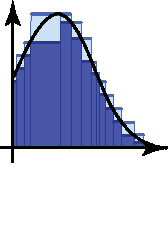
\includegraphics[trim=0cm 0cm 0cm 0cm, clip, scale=1.6]{images/lebesgueriemann1}
	\end{center}
\end{minipage}
\begin{minipage}{0.5\textwidth}
	\begin{center}
		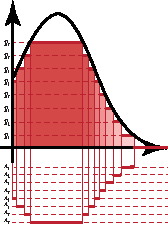
\includegraphics[trim=0cm 0cm 0cm 0cm, clip, scale=1.6]{images/lebesgueriemann2}
	\end{center}
\end{minipage}\\
In \textit{Sur le development de la notion d'intégrale (1926)} Lebesgue ripercorre il procedimento naturale alla base di questa idea fondamentale:
\blockquote{
	‘‘I geometri del diciassettesimo secolo considerano l'integrale di $f(x)$ - la parola \textit{integrale} non era ancora stata inventata, ma non importa - come la somma di un'infinità di indivisibili, ognuno dei quali era l'ordinata, positiva o negativa, di $f(x)$.\\
	Benissimo! Noi abbiamo semplicemente raggruppato insieme gli \textit{indivisibili} di 	grandezza vicina. Abbiamo, come si dice in algebra, riunito termini simili. Si potrebbe dire che, secondo il procedimento di Riemann, si cerca di sommare gli indivisibili prendendoli \textit{nell’ordine nel quale ci sono forniti dalla variazione di $x$}, come un commerciante confusionario che conta monete e biglietti a caso,	nell’ordine in cui gli vengono dati, mentre noi operiamo come un commerciante metodico che dice:
	\begin{center}
		 \begin{tabular}{l}
			«ho $m(G_1)$ monete da $100$, che valgono $100\ m(G_1)$»\\
			«ho $m(G_2)$ monete da $500$, che valgono $500\ m(G_2)$»\\
			«ho $m(G_3)$ biglietti da $1000$, che valgono $1000\ m(G_3)$»\\
			...
		\end{tabular}
	\end{center}
	Tutto insieme ho
	\begin{equation*}
		S=100\ m(G_1) + 500 m(G_2)+ 1000 m(G_3)+\ldots
	\end{equation*}
	I due procedimenti porteranno di certo il commerciante allo stesso risultato perché per quanti soldi abbia c’è solo un numero finito di monete e di biglietti da contare. Ma per noi che dobbiamo sommare un numero infinito di indivisibilità la differenza dei due metodi è \textit{di capitale importanza}.''
}
In altre parole, per calcolare l'integrale (secondo Lebesgue) di una funzione:
\begin{itemize}
	\item Suddividiamo l'immagine in intervalli e per ognuno di essi consideriamo un \textit{peso} dato dall'\textit{estremo inferiore} dei valori assunti dalla funzione nel dato intervallo.
	\item Consideriamo le controimmagini degli intervalli e associamo a ciascuna un valore detto \textbf{misura}.
	\item Calcoliamo un'approssimazione \textit{per difetto} dell'integrale sommando le misure che abbiamo ottenuto - ciascuna moltiplicata per il corrispondente peso.
	\item Più fitta è la partizione iniziale, più accurato sarà il valore dell'integrale.
\end{itemize}
\begin{intuit}
Poiché partizioniamo i \textit{valori} che assume una funzione e non il dominio in sè e li riordiniamo, possiamo trasformare delle funzioni particolarmente patologiche in funzioni ‘‘carine'' dal punto di vista dell'integrazione e ci consente di integrarle.
\end{intuit}
Osserviamo che l'idea di Lebesgue è decisamente geniale: non solo risolve i casi patologici che hanno afflitto i matematici del XIX secolo, ma ci permette di rivoluzionare completamente il concetto di integrale: dato che la partizione è effettuata sul \textit{codominio}, le funzioni non necessariamente devono essere definite sui reali, ma possiamo integrare funzioni definite su altri tipi di insiemi, come i naturali!\\
Tuttavia, abbiamo prima bisogno di affrontare alcune questioni:
\begin{enumerate}
	\item Dato che il dominio può essere un insieme qualsiasi, le controimmagini $f^{-1}\left(\left[y_i,y_{i+1}\right]\right)$ degli intervalli $\left[y_i,y_{i+1}\right]$ che otteniamo dalla partizione \textit{non} sono in generale intervalli: che cos'è la loro \textbf{misura}?
	\item Su quali insiemi è \textit{definibile} una misura?
	\item Per quali funzioni $f$ è possibile definire l'\textit{integrale}?
\end{enumerate}
Possiamo immaginare, da quanto detto, che una misura sia una funzione che quantifica la dimensione - che sia una lunghezza, un'area o volendo anche una cardinalità - di insiemi. Sostanzialmente, ci sono tre elementi da definire:
\begin{enumerate}[label=(\Roman*)]
	\item Una famiglia di insiemi su cui è definita una misura, che chiameremo poco intuitivamente $\sigma$\textbf{-algebra}, e i suoi elementi, che saranno detti \textbf{insiemi misurabili}.
	\item Una classe di funzioni su cui definire l’integrale, le \textbf{funzioni misurabili}.
	\item Ultima, ma decisamente non per importanza, una \textbf{misura} per valutare l’ampiezza degli insiemi.
\end{enumerate}
\section{Algebre e $\sigma$-algebre}
\begin{define}[Algebra]
	Sia $X$ un insieme qualsiasi. La famiglia $\mathcal{M}$ di sottoinsiemi di $X$ è una \textbf{algebra} \index{algebra} se soddisfa i seguenti assiomi:
	\begin{enumerate}
		\item L'\textit{insieme stesso} sta nell'algebra:
		\begin{equation}
			X\in\mathcal{M}
		\end{equation}
		\item L'algebra è chiusa rispetto alla \textit{complementarizzazione}: \begin{equation}
			A\in\mathcal{M}\implies A^C\in\mathcal{M}
		\end{equation}
		\item L'algebra è chiusa rispetto alla \textit{unione finita}:
		\begin{equation}
			A_1,\ \ldots,\ A_n\in\mathcal{M}\implies A_1\cup\ldots\cup A_n\in\mathcal{M}
		\end{equation}
	\end{enumerate}
\end{define}
Di queste nuove strutture matematiche ci interessano in particolare quelle che soddisfano un ulteriore condizione: la chiusura rispetto all'\textit{unione numerabile}.
\begin{define}[{$\sigma$}-algebra, spazi e insiemi misurabili]
	Sia $X$ un insieme qualsiasi. La famiglia $\mathcal{M}$ di sottoinsiemi di $X$ è una $\sigma$\textbf{-algebra} \index{{$\sigma$}-algebra} se soddisfa i seguenti assiomi:
	\begin{enumerate}
		\item L'\textit{insieme stesso} sta nell'algebra:
		\begin{equation}
			X\in\mathcal{M}
		\end{equation}
		\item L'algebra è chiusa rispetto alla \textit{complementarizzazione}: \begin{equation}
			A\in\mathcal{M}\implies A^C\in\mathcal{M}
		\end{equation}
		\item La $\sigma$-algebra è chiusa rispetto alla \textit{unione numerabile}: \begin{equation}
			A_n\in\mathcal{M}\implies \bigcup_{n\geq 1}A_n\in\mathcal{M} 
		\end{equation}
	\end{enumerate}
La coppia $\left(X,\mathcal{M}\right)$ si dice \textbf{spazio misurabile}\index{spazio!misurabile} e gli insiemi che appartengono a $\mathcal{M}$ sono detti \textbf{insiemi misurabili}\index{insieme!misurabile}.
\end{define}
\begin{observe}~{}
	\begin{itemize}
		\item $\emptyset\in\mathcal{M}$ in quanto è il complementare dell'insieme $X$.
		\item La $\sigma$-algebra è chiusa rispetto all'\textit{intersezione numerabile}:
		\begin{equation*}
			A_n\in\mathcal{M}\implies \bigcap_{n\geq 1}A_n\in\mathcal{M} 
		\end{equation*}
		Infatti, l'intersezione si può scrivere tramite unioni e complementari, operazioni interne alla $\sigma$-algebra, grazie alle \textit{leggi di De Morgan}\footnote{Nelle ‘‘Note aggiuntive'', a pagina \pageref{leggidemorgan} è possibile trovare alcune informazioni sulle leggi di De Morgan.}.
	\end{itemize}
\end{observe}
\begin{example}
	Ogni insieme si può dotare della struttura di spazio misurabile, in quanto ammette almeno la $\sigma$-algebra triviale data da $\setpart{X}$.
\end{example}
\begin{define}[{$\sigma$}-algebra generata da una famiglia di sottoinsiemi]
	Data una famiglia $\mathcal{F}$ di sottoinsiemi di $X$, si dice $\sigma$-\textbf{algebra generata da} $\mathcal{F}$\index{{$\sigma$}-algebra!generata da una famiglia di sottoinsiemi} l'intersezione di \textit{tutte} le $\sigma$-algebre che contengono $\mathcal{F}$ ed è la più piccola $\sigma$-algebra che contiene $\mathcal{F}$.
\end{define}
\begin{example}
	Se $X$ è spazio \textit{topologico} e $\mathcal{F}$ è la famiglia degli \textit{aperti} di $X$ (che coincide con la \textit{topologia} $\tau$ se definita con gli assiomi degli aperti), la $\sigma$-algebra generata da $\mathcal{F}$ si chiama $\sigma$\textbf{-algebra dei Boreliani di} $X$\index{{$\sigma$}-algebra!dei Boreliani} e si indica con $\mathcal{B}(x)$.\\
	Osserviamo che la famiglia $\mathcal{F}$ di per sé non è una $\sigma$-algebra: se $A$ è aperto, $A^C$ è chiuso e quindi non appartiene a $\mathcal{F}$; invece, in $\mathcal{B}(x)$ ci stanno anche i chiusi della topologia e quindi la complementarizzazione è un'operazione interna.
\end{example}
\section{Funzioni misurabili}
\begin{define}[Funzione misurabile]
	Sia $\left(X, \mathcal{M}\right)$ spazio misurabile e $Y$ spazio topologico. Una funzione $\funz{f}{X}{Y}$ si dice \textbf{misurabile}\index{funzione!misurabile} se \begin{equation}
		f^{-1}\left(A\right)\in\mathcal{M},\ \forall A\subseteq Y\text{ aperto.}
	\end{equation}
\end{define}
\begin{observe}
	Se $\mathcal{M}=\setpart{X}$, allora \textit{ogni} funzione è misurabile.
\end{observe}
\begin{examples}~{}
	\begin{enumerate}
		\item Sia $\left(X,\mathcal{B}(x)\right)$ spazio misurabile su $X$ spazio topologico con la $\sigma$-algebra dei Boreliani di $X$ e sia $Y$ spazio topologico. Allora
		\begin{center}
			$\funz{f}{X}{Y}$ continua$\implies \funz{f}{X}{Y}$ misurabile.
		\end{center}
	Infatti, $\forall A\subseteq Y$ aperto, $f^{-1}\left(A\right)$ è aperto per continuità di $f$ e quindi $f^{-1}\left(A\right)\in\mathcal{B}(x)$.
	\item Sia $\left(X,\mathcal{M}\right)$ spazio misurabile qualsiasi e sia $E\subseteq X$. Definiamo la \textbf{funzione caratteristica di} $E$\index{funzione!caratteristica di un sottoinsieme} o \textbf{indicatrice di} $E$\seeonlyindex{funzione!caratteristica di un sottoinsieme}{indicatrice di un sottoinsieme} la funzione
	\begin{equation}
		\funztot{\chi_E}{X}{\realset}{x}{\chi_E(x)=\begin{cases}
				\begin{array}{ll}
					1&\text{se }x\in E\\
					0&\text{se }x\notin E\\
				\end{array}
		\end{cases}}
	\end{equation}
Allora
\begin{center}
$\chi_E$ è misurabile $\iff E\in\mathcal{M}$
\end{center}
Infatti, preso $A\subseteq \realset$, si ha
\begin{equation*}
f^{-1}\left(A\right)=\begin{cases}
	\begin{array}{ll}
		\emptyset&\text{se }0\notin A,\ 1\notin A\\
		E^C&\text{se }0\in A,\ 1\notin A\\
		E&\text{se }0\notin A,\ 1\in A\\
		X&\text{se }0\in A,\ 1\in A
	\end{array}
\end{cases}
\end{equation*}
Allora $f^{-1}\left(A\right)\in\mathcal{M}\iff E\in\mathcal{M}$.
\end{enumerate}
\end{examples}
\begin{observe}
	La funzione caratteristica $\chi_{\rationalset\cap\left[0,1\right]}$ è la \textbf{funzione di Dirichlet}\footnote{Si veda pag. \pageref{funzionedirichlet}.}.
\end{observe}
\begin{propertiesqed}[Proprietà della funzioni misurabili]\label{funzionimisurabilicomplesse}~
	\begin{enumerate}
		\item Sia $\left(X,\mathcal{M}\right)$ uno spazio misurabile e sia $\funz{f}{X}{\complexset}$, dove $\complexset$ ha la topologia Euclidea. Possiamo ‘‘scomporre'' la funzione a valori complessi come combinazione lineare di funzioni reali rispetto alla base $(1,i)$.
		\begin{center}
			$\forall x\in X f(x)\in\complexset\implies f(x)=\underbrace{u(x)}_{\text{parte reale}}+i\underbrace{v(x)}_{\text{parte imm.}}$, con $\funz{u,v}{X}{\realset}$.
		\end{center}
	Allora
	\begin{enumerate}
		\item $f$ è misurabile$\implies u,\ v,\ \abs{f}$ misurabili.
		\item $u, v$ sono misurabili$\implies f=u+iv$ è misurabile.
	\end{enumerate}
\item Siano $\funz{f,g}{X}{\complexset}$. Se $f,g$ sono misurabili, allora
\begin{itemize}
	\item $f+g$ è misurabile.
	\item $fg$ è misurabile.\qedhere
\end{itemize}
\end{enumerate}
\end{propertiesqed}
\subsection{Caratterizzazione delle funzioni misurabili}
In \textsc{Calcolo delle Probabilità} abbiamo dato una definizione di funzione misurabile $\funz{f}{\left(X,\mathcal{M}\right)}{Y}$ se la controimmagine tramite $f$ di un Boreliano è un insieme misurabile per $\mathcal{M}$. Vedremo ora come questa definizione è equivalente a quella data all'inizio della sezione.
\begin{theoremasqed}[Caratterizzazione delle funzioni misurabili]~
	\begin{enumerate}\label{caratterizzazionefunzionimisurabili}
		\item La funzione $\funz{f}{\left(X,\mathcal{M}\right)}{Y}$, con $Y$ spazio topologico, è  misurabile se e solo se
		\begin{equation}
			f^{-1}\left(B\right)\in\mathcal{M},\ \forall B \text{ Boreliano di } Y.
		\end{equation}
		\item Posto $Y=\realset^{\ast}=\left[-\infty,+\infty\right]$, $\funz{f}{X}{\left[-\infty,+\infty\right]}$ è misurabile se e solo se
		\begin{equation}
			f\left(\left(\alpha,+\infty\right]\right)\in\mathcal{M},\ \forall \alpha\in\realset.\qedhere
		\end{equation}
	\end{enumerate}
\end{theoremasqed}
Che differenza c'è tra la definizione e le caratterizzazioni? In sostanza possono essere considerate tre ‘‘test'' differenti per mostrare o confutare che una funzione sia misurabile.
\begin{align*}
	\circled[red]{A}&\qquad f^{-1}\left(A\right)\in\mathcal{M},\ \forall A\text{ aperto di }Y\\
	\circled[red]{B}&\qquad f^{-1}\left(B\right)\in\mathcal{M},\ \forall B\text{ Boreliano di }Y\\
	\circled[red]{C}&\qquad f^{-1}\left(\left(\alpha,+\infty\right]\right)\in\mathcal{M},\ \forall \alpha\in\realset,\ \text{con }Y=\realset^{\ast}=\left[-\infty,+\infty\right]
\end{align*}
Da un punto di vista \textit{operativo} \circled[red]{B} non conviene come metodo per verificare che $f$ sia misurabile: i Boreliani, pur avendo la \textit{stessa cardinalità} degli aperti, li contengono \textit{strettamente}\footnote{A pag. \pageref{famigliediinsiemi} è possibile trovare un approfondimento sulla relazione tra Boreliani, aperti e altre classi di insiemi.} e quindi bisogna verificare ulteriori insiemi (come i chiusi) rispetto a quelli che si verificherebbero con la condizione \circled[red]{A}.\\
Tuttavia, \circled[red]{B} fornisce delle informazioni che immediatamente non si avevano dalla definizione originale: sono misurabili non solo le controimmagini degli aperti, ma anche le controimmagini dei chiusi.\\
Col caso \circled[red]{C} ci limitiamo ad operare in $\realset^{\ast}=\left[-\infty,+\infty\right]$, ma è sicuramente più vantaggioso da applicare rispetto ad \circled[red]{A}.
\subsection{Passaggio al limite per funzioni misurabili}
Ci chiediamo se, date $f_n$ successione di funzioni misurabili che convengono ad una funzione $f$ in \textit{una qualche} convergenza, $f$ risulta essere ancora misurabile e se sì, con quale tipo di convergenza.\\
A differenza di quanto visto col passaggio al limite della continuità, la risposta è affermativa anche sotto la sola ipotesi di \textit{convergenza puntuale}!\\
Per dimostrarlo (e lo faremo per funzioni a valori in $\complexset$), abbiamo bisogno di alcuni risultati preliminari che riguardano $\sup$, $\inf$, $\limsup$, $\liminf$ di una successione di funzione. Per poter parlare di $\limsup$ e $\liminf$ abbiamo bisogno di avere il codomini della funzione in uno spazio $Y$ con ordinamento, pertanto ci porremo in  $\realset^{\ast}=\left[-\infty,+\infty\right]$, ossia le nostre funzioni saranno del tipo
\begin{equation*}
\funz{f}{\left(X,\mathcal{M}\right)}{\realset^{\ast}=\left[-\infty,+\infty\right]}
\end{equation*}
\begin{define}[{$\sup$}, {$\inf$}, {$\limsup$} e {$\liminf$} di una successione di funzioni]
Sia $\funz{f_n}{\left(X,\mathcal{M}\right)}{\realset^{\ast}=\left[-\infty,+\infty\right]}$ misurabili.
Allora definiamo:
\begin{gather*}
	\left(\sup_{n\geq 1} f_n\right)(x)\coloneqq \sup_{n\geq 1}f_n(x),\ \forall x\in X\\
	\left(\inf_{n\geq 1} f_n\right)(x)\coloneqq \inf_{n\geq 1}f_n(x),\ \forall x\in X\\
	\left(\limsup_{n\to+\infty} f_n\right)(x)\coloneqq \limsup_{n\to+\infty}f_n(x),\ \forall x\in X\\
	\left(\liminf_{n\to+\infty} f_n\right)(x)\coloneqq \liminf_{n\to+\infty}f_n(x),\ \forall x\in X
\end{gather*}
\end{define}
\begin{proposition}[Misurabilità di {$\sup$}, {$\inf$}, {$\limsup$} e {$\liminf$} di una successione di funzioni misurabili]\label{misurabilitàsupinf}
	Sia $ \left(X,\mathcal{M}\right)$ uno spazio misurabile e siano $\funz{f_n}{\left(X,\mathcal{M}\right)}{\realset^{\ast}=\left[-\infty,+\infty\right]}$ misurabili.
	Allora
	\begin{equation*}
		\sup_{n\geq 1} f_n\quad\inf_{n\geq 1} f_n\quad\limsup_{n\to\infty} f_n\quad\liminf_{n\to\infty} f_n
	\end{equation*}
sono misurabili.
\end{proposition}
\begin{demonstration}~{}
	\begin{enumerate}
		\item Sia $\displaystyle g(x)=\sup_{n\geq 1} f_n(x),\ \forall x\in X$. Dobbiamo provare che $g$ sia misurabile, con $\funz{g}{\left(X,\mathcal{M}\right)}{\realset^{\ast}=\left[-\infty,+\infty\right]}$. Per il teorema \ref{caratterizzazionefunzionimisurabili} sulla \textit{caratterizzazione} delle funzioni misurabili è sufficiente dimostrare che $g^{-1}\left(\left(\alpha,+\infty\right]\right)\in\mathcal{M},\ \forall\alpha\in\realset$.\\
		Innanzitutto, mostriamo che
		\begin{equation*}
			g^{-1}\left(\left(\alpha,+\infty\right]\right)=\bigcup_{n\geq 1}f_n^{-1}\left(\left(\alpha,+\infty\right]\right),\ \forall \alpha\in\realset.
		\end{equation*}
	Infatti:
	\begin{align*}
		x\in g^{-1}\left(\left(\alpha,+\infty\right]\right)&\iff g(x)>\alpha\\
		& \iff \exists j\geq 1\colon f_j(x)>\alpha\\
		& \iff \exists j\geq x\in f_j^{-1}\left(\left(\alpha,+\infty\right]\right)\\
		& \iff x\in \bigcup_{n\geq 1}f_n^{-1}\left(\left(\alpha,+\infty\right]\right).
	\end{align*}
	Poiché $f_n$ è misurabile si ha
	\begin{equation*}
		f_n^{-1}\left(\left(\alpha,+\infty\right]\right)\in\mathcal{M}
	\end{equation*}
ed essendo $\mathcal{M}$ una $\sigma$-algebra è chiusa rispetto all'unione misurabile e dunque
	\begin{equation*}
	g^{-1}\left(\left(\alpha,+\infty\right]\right)=\bigcup_{n\geq 1}f_n^{-1}\left(\left(\alpha,+\infty\right]\right)\in\mathcal{M}
	\end{equation*}
	\item[2,3,4.] Si riconducono al caso $1)$ perché
	\begin{gather*}
		\inf_{n\geq 1}f_n=-\left(\sup_{n\geq 1}\left(-f_n\right)\right)\\
		\limsup_{n\to+\infty}f_n=\inf_{k\geq 1}\sup_{n\geq k}f_n\\
		\liminf_{n\to+\infty}f_n=\sup_{k\geq 1}\inf_{n\geq k}f_n\qedhere
	\end{gather*}
	\end{enumerate}
\end{demonstration}
\begin{corollary}[Passaggio al limite per funzioni misurabili in {$\complexset$}]
	Sia $\left(X,\mathcal{M}\right)$ uno spazio misurabile e siano $\funz{f_n}{X}{\complexset}$.\\
	Se $f_n$ sono misurabili ed esiste $\funz{f}{X}{\complexset}$ tale che
	\begin{equation*}
		\lim_{n\to+\infty}f_n(x)=f(x),\ \forall x\in X
	\end{equation*}
	allora $f$ è misurabile.
\end{corollary}
\begin{demonstration}
	Riconduciamoci al caso reale per utilizzare la proposizione precedente. Posto
	\begin{equation*}
		f_n=u_n+iv_n\qquad f=u+iv
	\end{equation*}
dove
\begin{equation*}
	\begin{array}{ll}
		\funz{u_n=\Re\left(f_n\right)}{X}{\realset}&\funz{v_n=\Im\left(f_n\right)}{X}{\realset}\\
		\funz{u=\Re\left(f\right)}{X}{\realset}&\funz{v=\Im\left(f\right)}{X}{\realset}
	\end{array}
\end{equation*}
Come visto nella proposizione \ref{funzionimisurabilicomplesse}, $f_n$ misurabile implica che sia $u_n$ sia $v_n$ siano misurabili e, dal risultato precedente sulle funzioni a valori in $\realset^{\ast}$ si ha
\begin{equation*}
	\limsup_{n\to+\infty}u_n,\ \limsup_{n\to+\infty}v_n\text{ misurabili.}
\end{equation*}
D'altra parte si ha
\begin{equation*}
	\lim_{n\to+\infty}f_n(x)=f(x)\implies
	\begin{cases}
		\displaystyle\lim_{n\to+\infty}u_n(x)=u(x)\\
		\displaystyle\lim_{n\to+\infty}v_n(x)=v(x)
	\end{cases}
\end{equation*}
Poiché i limiti esistono si ha
\begin{gather*}
	\lim_{n\to+\infty}u_n=\limsup_{n\to+\infty}u_n=u(x)\\	\lim_{n\to+\infty}v_n=\limsup_{n\to+\infty}v_n=v(x)
\end{gather*}
Quindi $u(x)$ e $v(x)$ sono misurabili, pertanto anche $f=u+iv$ è misurabile.
\end{demonstration}
\section{Misura di Peano-Jordan}
Negli stessi anni in cui si lavorò per espandere la classe di funzioni che ammettono integrale definito, diversi matematici lavorano su un'altra questione, quella della \textbf{misura} di un insieme.\\
Chiaramente già dall'antichità erano note misure di figure ‘‘elementari'', come ad esempio la lunghezza e l'area di un poligono o il volume di certi solidi, spesso sulla base di principi come quello di \textit{esaustione}.\\
Solo nel XIX secolo si cercò di formalizzare questi ragionamenti ed espandere il concetto di misura non soltanto a figure generiche, ma anche a più dimensioni fino ad arrivare ad una astrazione di tale concetto ad insiemi, indipendentemente dall'essere in $\realset^n$.\\
Il primo ad introdurre un concetto di misura di un sottoinsieme della retta, del piano o delle spazio fu Giuseppe \textbf{Peano} (1858-1932). Nel suo \textit{Applicazioni geometriche del
calcolo infinitesimale (1887)}, il matematico torinese ipotizza di ‘‘modernizzare'' il metodo di esaustione già citato in precedenza.
Ad esempio, prendo un insieme limitato in $\realset^2$, ossia quello che all'epoca veniva denominato \textit{campo piano}, potremmo considerare dei poligoni che contengono tale insieme - che chiameremo \textit{poligoni esterni} - e dei poligoni che sono contenuti in tale insieme - i cosiddetti \textit{poligoni interni}.
\begin{center}
	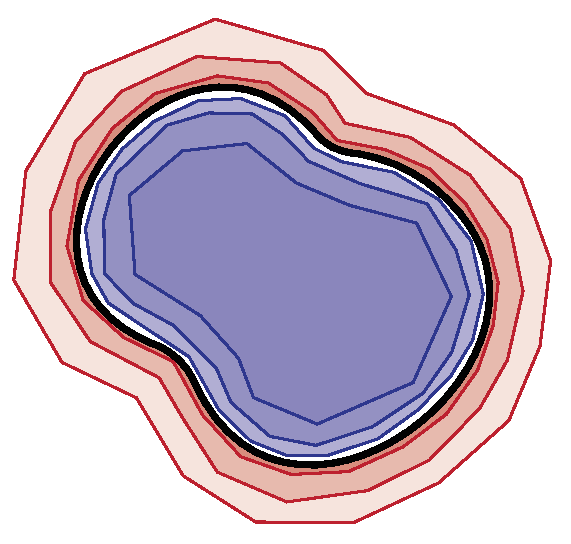
\includegraphics[trim=0cm 0cm 0cm 0cm, clip, scale=0.71]{images/peanopoligoni.pdf}
\end{center}
Se l'estremo inferiore dei poligoni esterni coincide con quello superiore di quelli interni, potremmo dire che l'insieme è misurabile e ha area pari a questo limite.
Inoltre, Peano fornisce una condizione necessaria e sufficiente: la differenza tra i poligoni esterni ed interni deve essere piccola a piacere, ossia la frontiera dell'insieme (che chiaramente è contenuta nell'area di piano fra i poligoni esterni ed interni) dovrà avere misura nulla.\\
Possono capitare anche insiemi che non ammettono area. 
\begin{example}
	Supponiamo di prendere tutti i punti a distanza \textit{razionale} $r\leq 1$ dall'origine, cioè infinite circonferenze di raggio razionale interne al disco di raggio 1.\\
	Chiaramente l'area interna è uguale a 0, mentre essendo l'insieme denso nel disco di raggio 1, ogni poligono che la contiene contiene il cerchio e quindi l'area esterna è maggiore o uguale 1: essendo l'area interna e l'area esterna diverse, il poligono non ammette aree.
\end{example}
La misura di Peano, per quanto innovativa, risente di alcuni problemi: parlare di poligoni o solidi poligonali è facile farlo in $\realset^2$ o $\realset^3$, ma non è generalizzabile in dimensioni maggiori: ad esempio, qual è la misura di un ipersolido poligonale di dimensione 4? Inoltre, la misura di Peano non è numerabilmente additiva, ossia un'unione \textit{infinita numerabile} di insiemi misurabili secondo Peano non è necessariamente ancora misurabile.\\
Qualche anno dopo i lavori di Peano, il matematico francese Marie Camille \textbf{Jordan} (1838-1922) \textit{estende} il concetto di misura introdotta da Peano a una generica dimensione $n$, utilizzando invece che poligoni o solidi poligoni delle \textit{unioni di intervalli}, \textit{rettangoli} o, in generale, \textit{parallelepipedi} $n$-dimensionali, poiché questi hanno una misura ben nota!
\begin{center}
	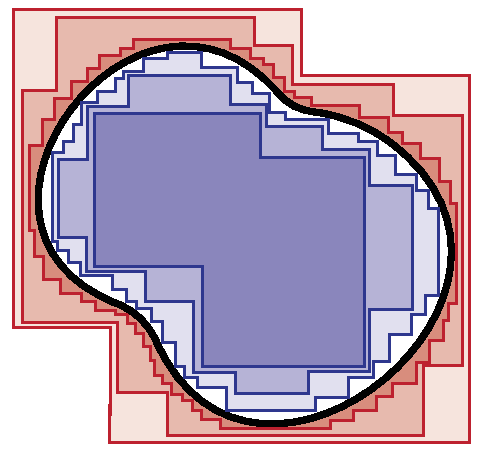
\includegraphics[trim=0cm 0cm 0cm 0cm, clip, scale=0.71]{images/peanoparallelepipedi.pdf}
\end{center}
Anche se questa misura coincide con quella di Peano (dopotutto, le unioni di parallelepipedi sono un \textit{caso particolare} di ipersolidi poligonali), in questo modo si risolve il \textit{primo problema} dei due problemi enunciati precedentemente; ciò nonostante, questa definizione non è ancora una misura numerabilmente-additiva.
\subsection{Definizione e osservazioni sulla misura di Peano-Jordan}
\begin{define}[Parallelepipedo {$n$}-dimensionale]
	Un \textbf{parallelepipedo}\index{parallelepipedo} $n$-dimensionale è un \textit{plurintervallo}, ossia un prodotto cartesiano di $n$ intervalli:
	\begin{equation}
		P=\prod_{i=1}^{n}\left[a_i,b_i\right]\quad\text{con }-\infty < a_i < b_i < +\infty
	\end{equation}
	Posta la \textbf{lunghezza}\index{lunghezza!di un intervallo} di un intervallo come
		\begin{equation}
			\mathcal{L}\left(\left[a_i,b_i\right]\right)=b_i-a_i
		\end{equation}
		la misura $n$-dimensionale del parallelepipedo è
		\begin{equation}
			V_n(P)=\prod_{i=1}^{n}\mathcal{L}\left(\left[a_i,b_i\right]\right)
		\end{equation}
	\end{define}
	Introduciamo formalmente la misura esterna e la misura interna di un insieme limitato $A$ come estremi inferiori e superiori di un \textbf{insieme elementare}\index{insieme!elementare}, cioè un'unione finita di parallelepipedi:
	\begin{itemize}
		\item \textsc{Misura esterna}:\index{misura!esterna} \begin{equation}
			m_{PJ}^X\left(A\right)=\inf\left\{\sum_{i=1}^{n}V_n\left(P_i\right)\mid P_i\text{ parallelepipedi},\ \bigcup_{i=1}^nP_i\supseteq A\right\}
		\end{equation}
		\item \textsc{Misura interna}:\index{misura!interna}
		\begin{equation}
			m_{PJ,X}\left(A\right)=\inf\left\{\sum_{i=1}^{n}V_n\left(P_i\right)\mid P_i\text{ parallelepipedi},\ \bigcup_{i=1}^nP_i\subseteq A\right\}
		\end{equation}
	\end{itemize}
	In generale $m_{PJ,X}\left(A\right)\leq m_{PJ}^{X}\left(A\right)$.
	\begin{define}[Misura di Peano-Jordan]
		Un insieme limitato $A$ è \textbf{misurabile secondo Peano-Jordan}\index{misura!secondo Peano-Jordan} se
		\begin{equation}
			m_{PJ}^X\left(A\right)=m_{PJ,X}\left(A\right)
		\end{equation}
	e la \textbf{misura} (secondo P-J) dell'insieme è
		\begin{equation}
			m_{PJ}\left(A\right)=m_{PJ}^X\left(A\right)=m_{PJ,X}\left(A\right)
		\end{equation}
	\end{define}
	\begin{propositionqed}[Criterio di misurabilità]
		L'insieme limitato $A\subseteq \realset^n$ è misurabile per Peano-Jordan se e solo se $\forall \epsilon>0,\ \exists P\subseteq A, Q\supseteq A$ con $P,\ Q$ insiemi elementari tali che
		\begin{equation}
			m_{PJ}\left(Q\right)-m_{PJ}(P)\leq \epsilon\qedhere
		\end{equation}
	\end{propositionqed}
	Definito
	\begin{equation}
		\mathcal{M}=\left\{A\subseteq \realset^n\mid A\text{è P-J misurabile}\right\}
	\end{equation}
	essa è un'\textit{algebra}, \textit{ma} non una $\sigma$-algebra, cioè non è chiusa rispetto all'unione \textit{numerabile infinita}.
	\begin{examplewt}[Controesempio dell'additività numerabile della misura di P-J]
		Consideriamo
		\begin{equation*}
			E=\rationalset\cap\left[0,1\right]=\bigcup_{n\geq 1}\left\{r_n\right\}
		\end{equation*}
		dove $\left\{r_n\right\}$ è un'enumerazione di razionali in $\left[0,1\right]$.\\
		$\left\{r_n\right\}$ è un punto e dunque è misurabile con misura nulla, ma \begin{equation*}
			\bigcup_{n\geq 1}\left\{r_n\right\}=E
		\end{equation*}
		\textit{non} è misurabile, dato che
		\begin{equation*}
			\begin{cases}
				m_{PJ}^X(E)=1\\
				m_{PJ,X}(E)=0
			\end{cases}
		\end{equation*}
	\end{examplewt}
	In altre parole, la misura secondo Peano-Jordan è \textit{additiva}, ma non $\sigma$-additiva.
	\begin{digression}
		Nella letteratura italiana si è soliti parlare ‘‘misura di Peano-Jordan'', quando in realtà questa terminologia è impropria, non essendo una \textit{misura} nel senso \textit{moderno} del termine. Nell'anglosfera lo stesso concetto viene chiamato ‘‘Jordan content'.
	\end{digression}
	\section{Misura secondo Lebesgue}
	Per quanto innovativa, la misura di Peano-Jordan presenta alcuni notevoli problemi:
	\begin{itemize}
		\item É definita solo per \textit{insiemi limitati}.
		\item Non è \textit{numerabilmente additività}: la misura di un'unione numerabilmente infinita di insiemi misurabili non è necessariamente misurabile.
	\end{itemize}
	Il concetto \textit{moderno} di misura di un sottoinsieme dello spazio $n$-dimensionale viene per la prima volta presentato in \textit{Intégrale, longueure, aire} (1902)
	dal matematico francese Henri \textbf{Lebesgue} (1875-1941) nell'ambito dell'annoso problema delle discontinuità nell'integrale definito.\\
	La costruzione della misura secondo Lebesgue inizia in modo analogo a quella di Peano-Jordan, definendo i \textit{parallelepipedi}; per poter definire la misurabilità di insiemi illimitati si ammettono parallelepipedi \textit{degeneri}.
	\begin{define}[Parallelepipedo {$n$}-dimensionale]
		Un \textbf{parallelepipedo}\index{parallelepipedo} $n$-dimensionale è un \textit{plurintervallo}, ossia un prodotto cartesiano di $n$ intervalli eventualmente \textit{degeneri}:
		\begin{equation}
			P=\prod_{i=1}^{n}\left[a_i,b_i\right]\quad\text{con }-\infty \leq a_i \leq b_i \leq +\infty
		\end{equation}
		Posta la \textbf{lunghezza}\index{lunghezza!di un intervallo} di un intervallo come
		\begin{equation}
			\mathcal{L}\left(\left[a_i,b_i\right]\right)=
			\begin{cases}
				\begin{array}{ll}
					b_i-a_i & \text{se }-\infty < a_i \leq b_i < +\infty\\
					+\infty&\text{altrimenti}
				\end{array}
			\end{cases}
		\end{equation}
		la misura $n$-dimensionale del parallelepipedo è
		\begin{equation}
			V_n(P)=\prod_{i=1}^{n}\mathcal{L}\left(\left[a_i,b_i\right]\right)
		\end{equation}
		con la convenzione che $0\cdot \infty =0$.
	\end{define}
	\begin{observe}
		Come mai $0\cdot \infty$ non è lasciato indeterminato, ma posto proprio uguale a 0?. Per capirlo, facciamo prima un esempio in dimensione 2; consideriamo il rettangolo degenere
		\begin{equation*}
			P=\left\{a_1\right\}\times\left(a_2,+\infty\right).
		\end{equation*}
		Esso è un sottoinsieme di $\realset^2$, ma ha chiaramente una sola dimensione: seppur come semiretta ha una lunghezza ben definita (e in tal caso sarebbe infinita tale lunghezza), è ragionevole dire che come oggetto \textit{bidimensionale} abbia \textit{area} $0$.
		\begin{center}
			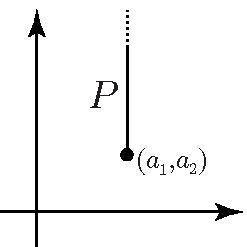
\includegraphics[trim=0cm 0cm 0cm 0cm, clip, scale=0.71]{images/rettangolodegenere.pdf}
		\end{center}
		In altre parole, se almeno un intervallo che compone il parallelepipedo $n$-dimensionale ha lunghezza nulla, $P$ è da intendersi come elemento di dimensione $k$ in uno spazio $n$-dimensionale, con $k< n$.
		In questo caso, la sua misura $n$\textit{-dimensionale} è nulla, anche se fosse \textit{illimitato} in diverse direzioni, da qui spiegato il perché di $0\cdot \infty =0$.
	\end{observe}
	A differenza di Peano-Jordan, Lebesgue definisce solamente la \textbf{misura esterna} dell'insieme:
	\begin{equation}
		m^X\left(A\right)=\inf\left\{\sum_{i=1}^{n}V_n\left(P_i\right)\middle| P_i\text{ parallelepipedi aperti},\ \bigcup_{i=1}^nP_i\supseteq A\right\}
	\end{equation}
dove per parallelepipedo \textit{aperti} si intende un plurintervallo definito da intervalli aperti.\\ 
	Essa si può vedere come una funzione
	\begin{equation}
		\funz{m^X}{\setpart{\realset^n}}{\left[0,+\infty\right]}
	\end{equation}
	che gode delle seguenti proprietà:
	\begin{itemize}
		\item Se l'insieme è un parallelepipedo $n$-dimensionale, la misura esterna del parallelepipedo ovviamente coincide con la misura $n$-dimensionale di esso:
		\begin{equation}
			m^X(P)=V_n(P),\ \forall P\text{ parallelepipedo}
		\end{equation}
		\item È \textit{monotona}:
		\begin{equation}
			m^X\left(A\right)\leq m^X\left(B\right),\ \forall A\subseteq B
		\end{equation}
		\item È $\sigma$-\textit{subadditiva}:
		\begin{equation}
			m^X\left(\bigcup_{n\geq 1}A_n\right)\leq \sum_{n\geq 1}m^X\left(A_n\right), \forall A_n\subseteq \realset^n
		\end{equation}
		\item È \textit{invariante per traslazioni}:
		\begin{equation}
			m^X\left(A+\left\{x\right\}\right)=m^X\left(A\right),\ \forall x\in\realset^n,\ \forall A\subseteq\realset^n
		\end{equation}
	\end{itemize}
	Osserviamo che per $m^X$ vale \textit{solo} la  $\sigma$-\textit{subadditività}, ma non la $\sigma$-\textit{additività}.
	\begin{define}[Insieme misurabile secondo Lebesgue {{\small (Criterio di Caratheodory)}}]\index{criterio!di Caratheodory}
		Un insieme $A\subseteq\realset^n$ è \textbf{misurabile secondo Lebesgue} se $\forall E\subseteq\realset^n$ vale
		\begin{equation}
			m_n^X(E)=m_n^X\left(E\cap A\right)+m_n^X\left(E\cap A^C\right)
		\end{equation}
	\end{define}
	$E$ è un \textbf{insieme test}\index{insieme!test} arbitrario (non necessariamente misurabile!): $A$ è misurabile se decompone bene $E$ in due sottoinsiemi misurabili $E\cap A$ e $E\cap A^C$.
	\begin{center}
		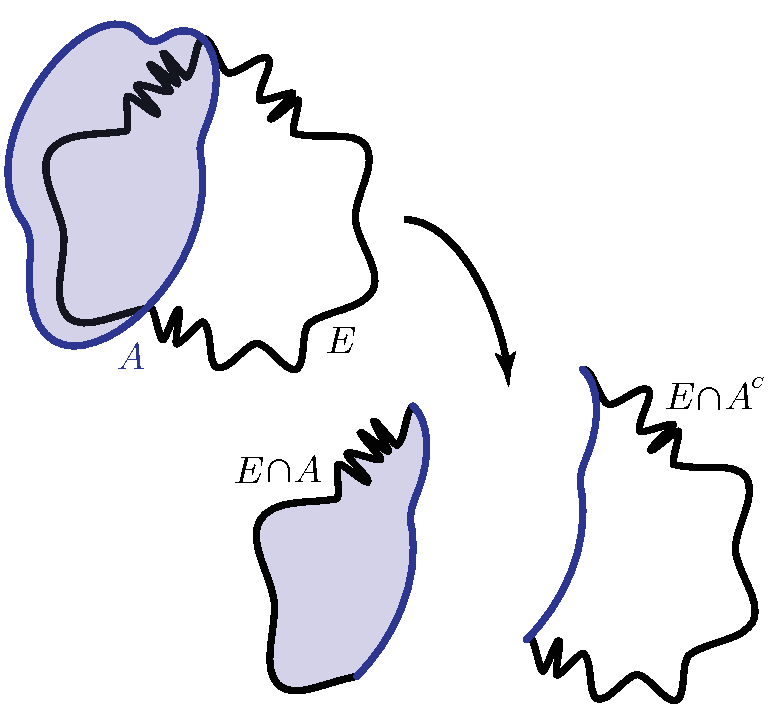
\includegraphics[trim=0cm 0cm 0cm 0cm, clip, scale=0.5]{images/criteriomisurabilita.pdf}
	\end{center}
	\begin{propositionqed}[Gli insiemi misurabili secondo Lebesgue sono una {$\sigma$}-algebra]
		La collezione di insiemi
		\begin{equation*}
			\mathcal{L}\left(\realset^n\right)=\left\{A\subseteq \realset^n\mid A\text{ è Lebesgue-misurabile}\right\}
		\end{equation*}
		è una $\sigma$-algebra.
	\end{propositionqed}
	\begin{define}[Misura secondo Lebesgue]
		La \textbf{misura secondo Lebesgue}\index{misura!secondo Lebesgue} è la restrizione della misura esterna a $\mathcal{L}\left(\realset^n\right)$:
		\begin{equation}
			m_n={m^X_n}\vert_{ \mathcal{L}\left(\realset^n\right)}\text{ ossia }\funz{m_n}{\mathcal{L}\left(\realset^n\right)}{\left[0,+\infty\right]}
		\end{equation}
	\end{define}
\subsection{Insiemi misurabili secondo Lebesgue}
La definizione data di insieme misurabile secondo Lebesgue non è particolarmente \textit{operativa}, in quanto richiede di controllare che un generico insieme test decomponga bene l'insieme di cui vogliamo verificare la misurabilità.
Di seguito presentiamo alcune classi importanti di insiemi misurabili secondo Lebesgue.
\begin{itemize}
	\item \textsc{\textbf{Insiemi elementari:}} (unioni di) parallelepipedi, anche degeneri:
	\begin{gather*}
		m_n(P)=V_n(P)\\
		m_n\left(\bigcup_{i=1}^{+\infty} P_i\right)=\sum_{i=1}^{+\infty}V_n\left(P_i\right)
	\end{gather*}
In particolare:
\begin{itemize}
	\item Preso $P=\realset^n$, allora $m_n\left(\realset^n\right)=+\infty$.
	\item Preso $P=\left\{x\right\},\ \forall x\in\realset^n$, allora $m_n\left(\left\{x\right\}\right)=0$.
\end{itemize}
\item \textsc{\textbf{Boreliani:}} $\mathcal{B}\left(\realset^n\right)\subsetneqq\mathcal{L}\left(\realset^n\right)$.\\
È importante sottolineare che ci sono insiemi misurabili \textit{non} Boreliani.\footnote{Si veda pag. \pageref{funzionecantor}.}
\item \textsc{\textbf{Tutti gli insiemi aventi misura \textit{esterna} nulla:}}
\begin{equation*}
	\forall A\subseteq \realset^n\ m_n^X\left(A\right)=0\implies A\in\mathcal{L}\left(\realset^n\right)\text{ e }m_n\left(A\right)=0
\end{equation*}
\end{itemize}

\begin{demonstration}
	Dobbiamo provare che $\forall E\subseteq \realset^n$
	\begin{equation*}
		m_n^X(E)=m_n^X\left(E\cap A\right)+m_n^X\left(E\cap A^C\right)
	\end{equation*}
	Ricordiamo che $m_n^X$ è $\sigma$-subadditiva e quindi finito-subadditiva, quindi
	\begin{equation*}
		E=\left(E\cap A\right)\cup \left(E\cap A^C\right)\implies m_n^X(E)\leq m_n^X\left(E\cap A\right)+m_n^X\left(E\cap A^C\right)
	\end{equation*}
	È sufficiente allora provare la disuguaglianza opposta. Osserviamo che $E\cap A^C\subseteq E$, dunque per monotonia di $m_n^X$ si ha
	\begin{equation*}
		m_n^X(E)\geq m_n^X\left(E\cap A^C\right)=m_n^X\left(E\cap A^C\right)+0=m_n^X\left(E\cap A^C\right)+m_n^X\left(E\cap A\right)
	\end{equation*}
	Infatti $E\cap A\subseteq A$ implica, per monotonia di $m_n^X$ che
	\begin{equation*}
		0\leq m_n^X\left(E\cap A\right)\leq m_n^X\left(A\right)=0
	\end{equation*}
	e quindi $m_n^X(E)\geq m_n^X\left(E\cap A^C\right)+m_n^X\left(E\cap A\right)$.
\end{demonstration}
\begin{attention}
	\textbf{Non} tutti gli insiemi sono misurabili! Se supponiamo vero l'Assioma della Scelta, l'\textbf{insieme di Vitali} è un insieme non misurabile in $\realset$ rispetto alla misura di Lebesgue unidimensionale\footnote{Si veda pag. \pageref{vitali} per la definizione dell'insieme di Vitali e la dimostrazione di ciò.}.
\end{attention}
Nella teoria di Lebesgue hanno un ruolo importante gli insiemi di misura nulla: esplicitiamo il legame tra misura nulla e cardinalità.
È noto che ogni singolo punto ha misura nulla; osserviamo che presa una famiglia di punti $\left\{x_n\right\}$ si ha
\begin{equation*}
	0\leq m_n\left(\bigcup_{n\geq 1}\left\{x_n\right\}\right)\leq \sum_{n\geq 1}m_n\left(\left\{x_n\right\}\right)=0
\end{equation*}
Ogni insieme \textbf{numerabile} è misurabile e ha misura nulla.
\begin{example}
	Posto $n=1$, ossia consideriamo la misura in $\realset$, si ha
	\begin{equation*}
		m_1\left(\rationalset\right)=0,\ m_1\left(\rationalset\cap\left[0,1\right]\right)=0
	\end{equation*}
\end{example}
\subsubsection{L'insieme (ternario) di Cantor}\label{insiemecantor}
Esistono anche insiemi di misura nulla con \textit{cardinalità del continuo}. Uno di questi è l'\textbf{insieme ternario di Cantor}, il quale possiede diverse proprietà interessanti e non particolarmente immediate. Esso si costruisce partendo dall'intervallo $\left[0,1\right]$ con il seguente procedimento iterativo:
\begin{itemize}
	\item \textbf{Passo 0.} È semplicemente l'intervallo $\left[0,1\right]$.
	\begin{center}
		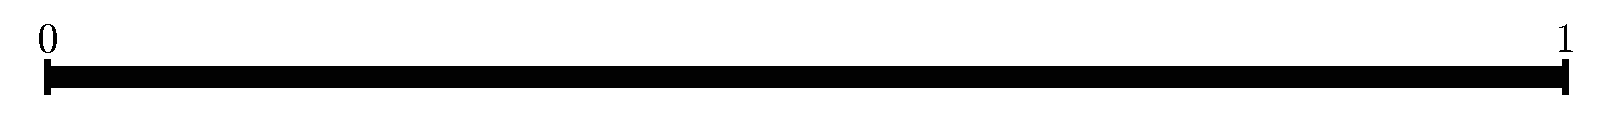
\includegraphics[trim=0cm 0cm 0cm 0cm, clip, scale=0.5]{images/Cantor0.pdf}
	\end{center}
	\item \textbf{Passo 1.} Suddividiamo $\left[0,1\right]$ in tre sottointervalli di ugual lunghezza
	\begin{equation*}
		I_1=\left[0,\nicefrac{1}{3}\right]\qquad I_2=\left(\frac{1}{3},\nicefrac{2}{3}\right)\qquad I_3=\left[\frac{2}{3},1\right]
	\end{equation*}
	e rimuoviamo l'intervallo aperto intermedio $I_2$, lasciando gli intervalli $I_1$ e $I_2$.
	\begin{center}
		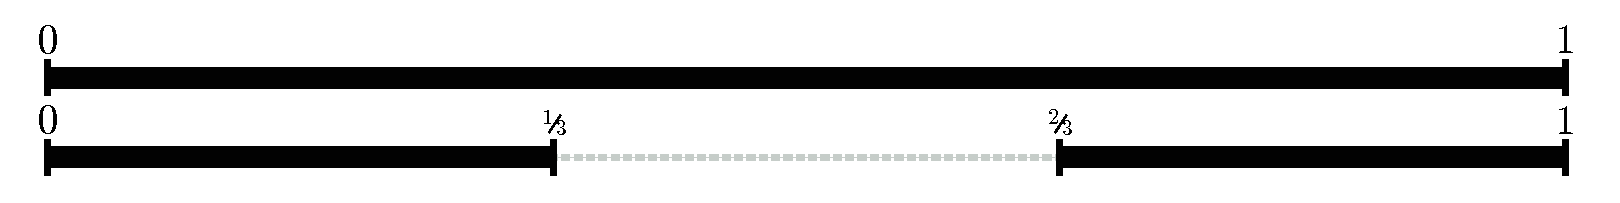
\includegraphics[trim=0cm 0cm 0cm 0cm, clip, scale=0.5]{images/Cantor1.pdf}
	\end{center}
	\item \textbf{Passo 2.} Prendiamo ciascun intervallo che avevamo al passo 1 e lo suddividiamo in modo analogo in tre parti uguali; per ciascun intervallo eliminiamo il sottointervallo aperto centrale, lasciando dunque 4 intervalli di lunghezza $\nicefrac{1}{9}$.
	\begin{center}
		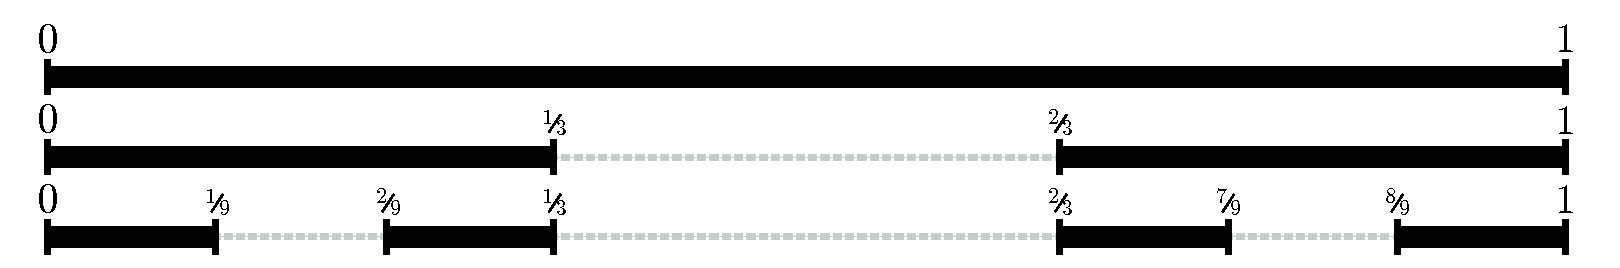
\includegraphics[trim=0cm 0cm 0cm 0cm, clip, scale=0.5]{images/Cantor2.pdf}
	\end{center}
	\item \textbf{Passo 3 e successivi.} Ripetiamo il procedimento del passo 2 con gli intervalli ottenuti nel passaggio precedente.
\begin{center}
	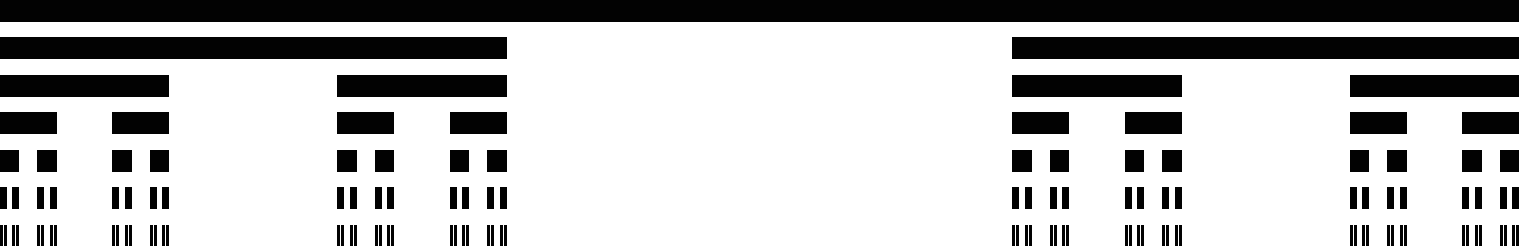
\includegraphics[trim=0cm 0cm 0cm 0cm, clip, scale=0.5]{images/Cantor3.pdf}
\end{center}
\end{itemize}
I punti che rimangono dopo infiniti passi è noto come \textbf{insieme di Cantor}\index{insieme!di Cantor} $C$.
\begin{equation*}
	C=\left[0,1\right]\setminus\bigcup_{n=0}^\infty \bigcup_{k=0}^{3^n-1} \left(\frac{3k+1}{3^{n+1}},\frac{3k+2}{3^{n+1}}\right)
\end{equation*}
Ci si potrebbe chiedere se ci sono ancora dei punti in questo insieme: dopotutto, abbiamo rimosso e rimosso continuamente degli intervalli. Sorprendentemente, dopo infiniti di questi passi ci sono ancora punti che rimangono, ma la peculiarità è che sono addirittura \textbf{non numerabili}!
\begin{theorema}[Innumerabilità dell'insieme di Cantor]
	Si denoti con $C$ l'insieme ternario di Cantor. Esiste una funzione suriettiva da $C$ in $\left[0,1\right]$; conseguentemente, $C$ ha la cardinalità del continuo.
\end{theorema}
\begin{demonstration}
	Ricordiamo che per ogni numero $x\in [0,1]$ esiste una successione $\{i_n\}_{n\geq 1}$ di interi, con $i_n\in \{0, 1, 2\}$, tale che 
	\begin{equation*}
		x=\sum_{n=1}^{+\infty} \dfrac{i_n}{3^n}. 
	\end{equation*}
	Tale successione è unica, tranne quando $x$ è della forma $q/3^n$, con  $q\in \naturalset$, nel qual caso esistono esattamente due successioni. Descriviamo l'insieme di Cantor $C$ usando questa rappresentazione in \textit{base tre}.
	\begin{itemize}
		\item Osserviamo che $\nicefrac{1}{3}$ si scrive come $0.1_3$ e $\nicefrac{2}{3}$ si scrive come $0.2_3$. Il \textit{primo intervallo} rimosso nella costruzione dell'insieme di Cantor consiste quindi di tutti i numeri del tipo $0.1abc\ldots_3$, dove $abc\ldots$ è una qualsiasi sequenza di numeri diversi dalle sequenze estreme $0000\ldots$ e $222\ldots$. I numeri residui dopo il primo passo della costruzione di $C$ sono esattamente quelli scrivibili come $0.0abc\ldots_3$ e $0.2abc\ldots_3$.
		\item Al secondo passo si rimuovono tutti i numeri del tipo $0.01abc\ldots_3$ e $0.21abc\ldots_3$.
	\end{itemize}
	Segue che i numeri che non vengono mai rimossi e che quindi appartengono all'insieme $C$ sono esattamente quelli che possono essere scritti come $0.abc\ldots_3$ usando solo le cifre $0$ e $2$.\\
	Definiamo ora una funzione $\funz{f}{C}{\left[0,1\right]}$ associando ad ogni elemento di $C$ scritto come $0.abc\ldots_3$, dove le cifre decimali sono solo $0$ e $2$, il numero di $\left[0,1\right]$ la cui rappresentazione in base due è quella ottenuta dalla sequenza $0.abc\ldots$ sostituendo ogni cifra $2$ con la cifra $1$.\\
	La funzione $f$ è chiaramente suriettiva: dato un numero $x\in \left[0,1\right]$, la sua controimmagine mediante $f$ è l'elemento dell'insieme di Cantor la cui rappresentazione decimale ternaria si ottiene dalla rappresentazione binaria di $x$ sostituendo ogni cifra $1$ con la cifra $2$.\\
	L'esistenza di una funzione suriettiva da $C$ in $\left[0,1\right]$ implica\footnote{In ‘‘Brevi cenni di teoria degli insiemi'', a pag. \pageref{cardinalitàsuriettiva} è possibile trovare maggiori dettagli su questa proprietà.} che la cardinalità di C è maggiore o uguale a quella di $\left[0,1\right]$:
	\begin{equation*}
		\abs{C}\geq \abs{X} 
	\end{equation*}
	D'altra parte, $C\subseteq \left[0,1\right]$ e dunque\footnote{In ‘‘Brevi cenni di teoria degli insiemi'', a pag. \pageref{cardinalitàinclusione} è possibile trovare maggiori dettagli su questa proprietà.} la sua cardinalità è minore o uguale a quella di $\left[0,1\right]$.
	\begin{equation*}
		\abs{C}\leq\abs{X}
	\end{equation*}
	Concludiamo quindi che $C$ e $\left[0,1\right]$ hanno la stessa cardinalità e dunque $C$ ha la cardinalità del continuo $\mathfrak{c}$.
\end{demonstration}
\begin{digression}
	Si noti che l'insieme di Cantor è un \textbf{frattale}\index{frattale}, dato che è sempre uguale a due copie di se stesso, se ogni copia è ristretta di un terzo e traslata.
\end{digression}
Pur essendo non numerabile esso ha lunghezza nulla. Nello specifico, consideriamo la misura di Lebesgue $m_1$ e ripercorriamo i passaggi della costruzione dell'insieme di Cantor:
\begin{itemize}
	\item \textbf{Passo 0.} $C_0$ coincide con l'intervallo $\left[0,1\right]$:
	\begin{equation*}
		m_1\left(C_0\right)=1
	\end{equation*}
	\item \textbf{Passo 1.} Togliamo un segmento di lunghezza $\nicefrac{1}{3}$ da un segmento di lunghezza $1$:
	\begin{equation*}
		m_1\left(C_1\right)=m_1\left(C_0\right)-\frac{1}{3}=\frac{2}{3}
	\end{equation*}
	\item \textbf{Passo 2.} Togliamo dei segmenti di lunghezza complessiva $\nicefrac{2}{9}$ da un'unione di segmenti di lunghezza $\nicefrac{2}{3}$:
	\begin{equation*}
		m_1\left(C_2\right)=m_1\left(C_1\right)-\frac{2}{9}=\frac{2}{3}-\frac{2}{9}=\frac{4}{9}
	\end{equation*}
\end{itemize}
Ad ogni passo l'insieme ha sempre lunghezza $\nicefrac{2}{3}$ quello del precedente. Al passo $n$-esimo si ha
\begin{equation*}
	m_1\left(C_n\right)=\left(\frac{2}{3}\right)^n
\end{equation*}
Poiché l'insieme di Cantor è prodotto dopo infiniti passi, allora
\begin{equation*}
	m_1\left(C\right)=\lim_{n\to+\infty}m_1\left(C_n\right)=\lim_{n\to+\infty}\left(\frac{2}{3}\right)^n=0
\end{equation*}
\subsection{Regolarità della misura di Lebesgue}
Ora enunciamo una proprietà della misura di Lebesgue, detta \textbf{regolarità}\index{regolarità!della misura di Lebesgue}.
\begin{theorema}[Regolarità della misura di Lebesgue]\label{regolaritàlebesgue}
	Le seguenti affermazioni sono equivalenti:
	\begin{enumerate}
		\item $E\in\mathcal{L}\left(\realset^n\right)$.
		\item $\forall \epsilon > 0,\ \exists A_{\epsilon}$ aperto di $\realset^n$ tale che
		\begin{itemize}
			\item $E\subseteq A_{\epsilon}$.
			\item $m^{X}_n\left(A_{\epsilon}\setminus E\right)<\epsilon$.
		\end{itemize}
		\item $\exists B$ Boreliano di $\realset^n$ tale che
	\begin{itemize}
		\item $E\subseteq B$.
		\item $m^{X}_n\left(B\setminus E\right)=0$.
	\end{itemize}
	\item $\forall \epsilon > 0,\ \exists C_{\epsilon}$ chiuso di $\realset^n$ tale che
	\begin{itemize}
		\item $E\supseteq C_{\epsilon}$.
		\item $m^{X}_n\left(E\setminus C_{\epsilon}\right)<\epsilon$.
	\end{itemize}
	\item $\exists D$ Boreliano di $\realset^n$ tale che
	\begin{itemize}
		\item $E\supseteq D$.
		\item $m^{X}_n\left(E\setminus D\right)=0$.
	\end{itemize}~\\
	\begin{minipage}{0.4\textwidth}
	\begin{center}
		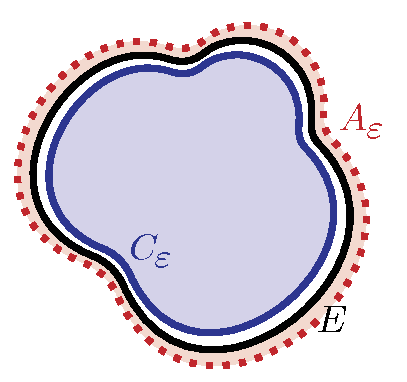
\includegraphics[trim=0cm 0cm 0cm 0cm, clip, scale=0.7]{images/regolarita1}\\
		\textbf{Caso 2. + 4.}
	\end{center}
\end{minipage}
\begin{minipage}{0.5\textwidth}
	\begin{center}
			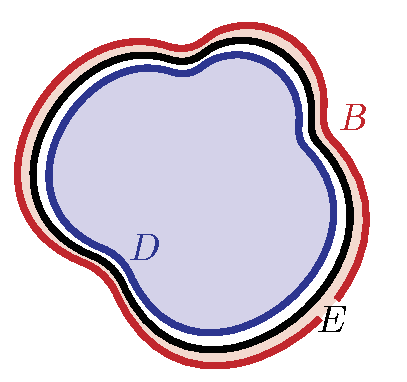
\includegraphics[trim=0cm 0cm 0cm 0cm, clip, scale=0.7]{images/regolarita2}\\
			\textbf{Caso 3. + 5.}
	\end{center}
\end{minipage}
	\end{enumerate}
\end{theorema}
\begin{demonstration}
	Dimostriamo le catene di implicazioni
	\begin{equation*}
		\mathbf{(i)\implies (ii)\implies (iii)\implies (i)\qquad(i)\implies (iv)\implies (v)\implies (i)}
	\end{equation*}
$\mathbf{(i)\implies(ii)}\quad$ Consideriamo il caso $m_n(E)<+\infty$. Per definizione di $m^{X}_n$ e di $\inf$, fissato $\epsilon >0$ $E$ è contenuto in un ricoprimento di parallelepipedi aperti tale che
\begin{equation*}
	\sum_{i=1}^{+\infty}V_n\left(P_i\right)<m_n(E)+\epsilon
\end{equation*}
dunque, posto
\begin{equation*}
	A=\bigcup_{n\in\naturalset}P_n,
\end{equation*}
l'aperto $A$ verifica, per subadditività numerabile,
\begin{equation*}
	m_n\left(A\right)<m_n(E)+\epsilon
\end{equation*}
e dal fatto che $m_n(E)<+\infty$ segue allora % aggiungere tabella proprietà in footnotes
\begin{equation*}
	m_n\left(A\setminus E\right)=m_n\left(A\right)-m_n(E)<\epsilon
\end{equation*}
Sia ora $m_n(E)=+\infty$. Possiamo vederlo come la seguente unione:
\begin{equation*}
	E=\bigcup_{i=1}^{+\infty}\left(E\cap Q_i\right),
\end{equation*}
dove $Q_i$ è una famiglia di parallelepipedi privi di punti interni comuni (ossia che hanno in comune al più i bordi), la cui unione sia $\realset^n$. Dato che $m_n\left(E\cap Q_n\right)<m_n(E)<Q$, per quanto già dimostrato esistono degli $A_i\supseteq E\cap Q_i$ tali che
\begin{equation*}
	m_n\left(A_i\setminus\left(E\cap Q_i\right)\right)<\frac{\epsilon}{2^{i+1}},\ \forall i\in\naturalset
\end{equation*}
Allora possiamo prendere come aperto
\begin{equation*}
	A=\bigcup_{i=1}^{+\infty}A_i.
\end{equation*}
Esso contiene $E$, e poiché
\begin{equation*}
	A\setminus E=\left(\bigcup_{i=1}^{+\infty}A_i\right)\setminus\left(\bigcup_{i=1}^{+\infty}\left(E\cap Q_i\right)\right)\subseteq\bigcup_{i=1}^{+\infty}\left(A_i\setminus\left(E\cap Q_i\right)\right)
\end{equation*}
si conclude che
\begin{equation*}
	m_n\left(A\setminus E\right)<\sum_{i=1}^{+\infty}m_n\left(A_i\setminus\left(E\cap Q_i\right)\right)<\epsilon
\end{equation*}
$\mathbf{(ii)\implies(iii)}\quad$ Per ogni $i\in\naturalset$, sia $A_i$ un aperto contenente $E$, tale che
\begin{equation*}
	m^{X}_n\left(A_i\setminus E\right)<\frac{1}{i+1}.
\end{equation*}
L'insieme
\begin{equation*}
	B=\bigcap_{i=1}^{+\infty}A_i
\end{equation*}
è un Boreliano contenente $E$ e si ha, per monotonia,
\begin{equation*}
	m_n^{X}\left(B\setminus E\right)\leq m_n^{X}\left(A_i\setminus E\right)<\frac{1}{n+1},\ \forall i\in \naturalset
\end{equation*}
cioè $m_n^{X}\left(B\setminus E\right)=0$.\\
$\mathbf{(iii)\implies(i)}\quad$  Scrivendo $E=B\setminus\left(B\setminus E\right)$, la tesi segue dal fatto che l'insieme $B$ è misurabile perché boreliano, mentre l'insieme $B\setminus E$ è misurabile avendo, per ipotesi, misura esterna nulla. Dunque $E$ è misurabile.\\
$\mathbf{(i)\implies(iv)\implies(v)\implies(i)}\quad$ Queste implicazioni si dimostrano facilmente applicando ad $E^C$ gli enunciati già dimostrati. 
\end{demonstration}
\begin{observe}
	Dai punti 2 e 4 si può caratterizzare un insieme $E$ misurabile secondo Lebesgue come un insieme che \textit{differisce poco}, in termini della misura esterna, sia da aperti contenenti $E$, sia da chiusi contenuti in $E$.\\
	Dai punti 3 e 5, invece, si può vedere ogni insieme misurabile secondo Lebesgue come un Boreliano a cui abbiamo tolto o aggiunto, rispettivamente, un insieme di misura nulla. Nello specifico, dal punto 5,
	\begin{equation*}
		E=D\cup\left(E\setminus D\right)
	\end{equation*}
\end{observe}
\subsection{Confronto tra la misura di Peano-Jordan e di Lebesgue}
Come abbiamo visto, la misura di Peano-Jordan soddisfa solo alcune proprietà della misura in senso assiomatico, essendo $\sigma$-subadditiva, mentre la misura secondo Lebesgue è a tutti gli effetti una misura assiomatica moderna. Ci si può dunque chiedere se tali concetti sono incompatibili tra di loro oppure se c'è una qualche relazione tra di esse.\\
È già noto che non tutti gli insiemi misurabili secondo Lebesgue lo sono secondo Peano-Jordan.
\begin{example}
	Consideriamo $E=\rationalset\cap\left[0,1\right]$.
	\begin{itemize}
		\item $E$ numerabile implica che $E$ è Lebesgue-misurabile e $m_1(E)=0$.
		\item $E$ \textit{non} è Peano-Jordan misurabile, in quanto
		\begin{equation*}
			m_{PJ}^{X}(E)=1\neq 0=m_{PJ,X}(E)
		\end{equation*}
	\end{itemize}
\end{example}
Invece, si vede banalmente che gli insiemi elementari, ossia le unioni di parallelepipedi $n$-dimensionali, sono misurabili sia secondo Lebesgue, sia secondo Peano-Jordan (a patto di fare un'unione finita di elementi); in particolare, le misure coincidono.
\begin{gather*}
	m_{PJ}(P)=m_n(P)=V_n(P)\\
	m_{PJ}\left(\bigcup_{i=1}^{k}P_i\right)=m_n\left(\bigcup_{i=1}^{k}P_i\right)=\sum_{i=1}^{k}V_n\left(P_i\right)
\end{gather*}
Il seguente teorema ci afferma un risultato importante: \textit{tutti} gli insiemi misurabili secondo Peano-Jordan sono misurabili secondo Lebesgue e le misure in tal caso coincidono.
\begin{theorema}[Misurabile secondo Peano-Jordan implica misurabile secondo Lebesgue]
	Sia $E\subseteq\realset^n$ limitato. Allora
	\begin{enumerate}
		\item Se $E$ è Peano-Jordan misurabile allora $E$ è Lebesgue-misurabile.
		\item Se vale ciò, allora $m_{PJ}(E)=m_n(E)$.
	\end{enumerate}
\end{theorema}
\begin{demonstration}
	Dimostriamo il punto 1. Sia $E\subseteq \realset^n$ e Peano-Jordan misurabile. Per provare che $E$ è misurabile secondo Lebesgue useremo il teorema di \textit{regolarità} precedentemente dimostrato.\\
	In particolare, proviamo che $\forall \epsilon >0\ \exists A_{\epsilon}$ aperto tale che
	\begin{itemize}
		\item $E\subseteq A_{\epsilon}$.
		\item $m_n^{X}\left(A_{\epsilon}\setminus E\right)<\epsilon$.
	\end{itemize}
Sappiamo che $E$ è misurabile secondo Peano-Jordan, dunque per il criterio equivalente $\forall \epsilon >0,\ \exists A_{\epsilon},\ B_{\epsilon}$ unioni finite di parallelepipedi con $B_{\epsilon}\subseteq E\subseteq A_{\epsilon}$ tali che $m_{PJ}\left(A_{\epsilon}\setminus B_{\epsilon}\right)<\epsilon$. Allora l'insieme $A_{\epsilon}$ così definito è proprio quello che stavamo cercando. Noto innanzitutto che $A_{\epsilon}\setminus E\subseteq A_{\epsilon}\setminus B_{\epsilon}$, per monotonia della misura esterna otteniamo:
\begin{equation*}
	m_{n}^{X}\left(A_{\epsilon}\setminus E\right)<	m_{n}^{X}\left(A_{\epsilon}\setminus B_{\epsilon}\right)=m_{PJ}^X\left(A_{\epsilon}\setminus B_{\epsilon}\right)=m_{PJ}\left(A_{\epsilon}\setminus B_{\epsilon}\right)<\epsilon\qedhere
\end{equation*}
\end{demonstration}
\section{Definizione assiomatica di misura}
La definizione di misura di Lebesgue che abbiamo analizzato nella scorsa sezione non è esattamente la stessa che il matematico francese diede nella sua tesi di laurea, bensì una rielaborazione successiva con alcune modifiche; nello specifico, la trattazione moderna viene inquadrata nella teoria \textbf{assiomatica} della misura, introdotta già prima di Lebesgue da Emil \textbf{Borel} (1871-1956) in \textit{Léçons sur la théorie des fonctions (1898)}.\\
I concetti di $\sigma$-algebra e insieme misurabile che abbiamo già affrontato si possono ricondurre proprio a Borel, così come la seguente \textit{definizione assiomatica} di misura.
\begin{define}[Misura e spazio di misura]
	Dato $\left(X,\mathcal{M}\right)$ uno spazio misurabile, una funzione $\funz{\mu}{\mathcal{M}}{\realset^{\ast}=\left[-\infty,+\infty\right]}$ è detta \textbf{misura}\index{misura} se soddisfa le seguenti proprietà:
	\begin{itemize}
		\item \textsc{\textbf{Non negatività:}} $\forall A\in\mathcal{M},\ \mu\left(A\right)\geq 0$.
		\item \textsc{\textbf{Insieme vuoto nullo:}} $\mu\left(\emptyset\right)=0$.
		\item $\sigma$-\textsc{\textbf{additività:}} $\forall A_n\in\mathcal{M}$ tali che $A_i\cap A_j=\emptyset\ \forall i\neq j$, allora
		\begin{equation}
			\mu\left(\coprod_{n\geq 1}A_n\right)=\sum_{n\geq 1}\mu\left(A_n\right)
		\end{equation}
	\end{itemize}
	In tal caso la terna $\left(X,\mathcal{M},\mu\right)$ è detta \textbf{spazio di misura}\index{spazio!di misura}.
	\begin{itemize}
		\item $\mu$ si dice \textbf{completa}\index{misura!completa} se $\forall S\subseteq N,\ \forall N\in\mathcal{M}\colon\mu(N)=0\implies S\in\mathcal{M}$ e $\mu(S)=0$.
		\item $\mu$ si dice \textbf{finita}\index{misura!finita} se $\mu(x)<+\infty$.
		\item $\mu$ si dice $\sigma$-\textbf{finita}\index{misura!$\sigma$-finita} se
		\begin{itemize}
			\item $\mu(x)=+\infty$.
			\item $\displaystyle X=\bigcup_{n\geq 1}X_n$, con $X_n\in\mathcal{M}$ tale che $\mu\left(X_n\right)\leq +\infty$.
		\end{itemize}
	\item $\mu$ si dice \textbf{di probabilità}\index{misura!di probabilità} se $\mu(x)=1$.
	\end{itemize}
\end{define}
\begin{observe}
	Ogni misura può essere opportunamente essere resa completa estendendo la $\sigma$-algebra di definizione.
\end{observe}
\begin{exampleswt}[Spazi di misura]~{}
	\begin{enumerate}
		\item $\left(\realset^n,\mathcal{L}\left(\realset^n\right)\right)$ è spazio di misura con la \textbf{misura di Lebesgue}
		\begin{equation}
			\funz{m_n}{\mathcal{L}\left(\realset^n\right)}{\left[0,+\infty\right]}
		\end{equation}
		Osserviamo che $m_n$ è $\sigma$-finita perché $m_n\left(\realset^n\right)=+\infty$ con
		\begin{equation*}
			\realset^n=\bigcup_{n\geq 0}B_n\left(0\right)\quad\text{con }m_n\left(B_n\left(0\right)\right)<+\infty
		\end{equation*}
		Inoltre, essa è \textbf{completa}. % to do: aggiungere dim completa?
		\item Fissato $x_0\in X$ insieme qualunque, $\left(X,\setpart{X}\right)$ è uno spazio di misura con la funzione $\delta$ \textbf{di Dirac concentrata in} $x_0$\index{Delta di Dirac}:
		\begin{equation}
			\funztot{\delta}{\setpart{X}}{\left[0,+\infty\right]}{E}{\begin{cases}
					\begin{array}{ll}
						1&\text{se }x_0\in E\\
						0&\text{se }x_0\notin E
					\end{array}
			\end{cases}}
		\end{equation}
		\item Preso $X$ insieme qualunque e scelti
		\begin{itemize}
			\item $\left\{x_n\right\}_{n\geq 0}$ una famiglia di elementi di $X$.
			\item $p_n\geq 0, \forall n\geq 0$ dei \textbf{pesi}\index{peso}.
		\end{itemize}
	allora $\left(X,\setpart{X}\right)$ è spazio di misura con la \textbf{misura di conteggio pesata}\index{misura!di conteggio!pesata}:
	\begin{equation}
		\funztot{\mu}{\setpart{X}}{\left[0,+\infty\right]}{E}{\displaystyle\sum_{n\colon x_n\in E}p_n}
	\end{equation}
Se
\begin{equation*}
	\sum_{n\colon x_n\in E}p_n=1,
\end{equation*}
$\mu_p$ è una \textbf{misura di probabilità discreta}\index{misura!di probabilità!discreta}, come la m.d.p. \textit{binomiale}, di \textit{Poisson}, ecc...\\
\item Preso $X=\naturalset$, i punti $x_n=n, \forall n\geq 1$ e $p_n=1,\ \forall n\geq 1$, allora $\left(\naturalset,\setpart{\naturalset}\right)$ è spazio di misura con la \textbf{misura di conteggio semplice}\index{misura!di conteggio!semplice}, un caso particolare dell'esempio precedente:
	\begin{equation}
	\forall E\subseteq\naturalset,\ \mu(E)=\sum_{n\colon n\in E}1=\begin{cases}
		\begin{array}{ll}
			\# E&\text{se }E\text{ finito}\\
			+\infty&\text{se }E\text{ infinito}
		\end{array}
	\end{cases}
\end{equation}
	\end{enumerate}
\end{exampleswt}
\begin{property}[Continuità della misura]
	Sia $\left(X,\mathcal{M}\right)$ uno spazio misurabile, $\funz{\mu}{\mathcal{M}}{\left[0,+\infty\right]}$ una misura. Allora $\mu$ è una funzione \textbf{continua da sopra e da sotto} - dove la continuità è quella delle funzioni definite su una collezione di insiemi:
	\begin{itemize}
		\item Per ogni successione di insiemi $A_n$ \textit{crescente}, cioè tale che $A_i\subseteq A_{i+1},\ \forall i\in\naturalset$, si ha
		\begin{equation}
			\mu\left(\bigcup_{n\geq 1}A_n\right)=\lim_{n\to+\infty}\mu\left(A_n\right)
		\end{equation}
		e $\mu$ è detta \textbf{continua da sotto}\index{continuità!da sotto}. 
	\begin{center}
		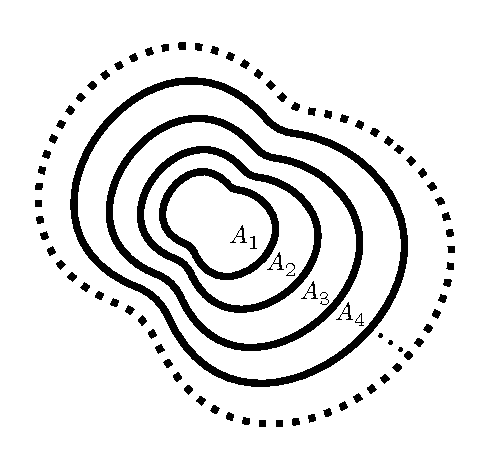
\includegraphics[trim=0cm 0cm 0cm 0cm, clip, scale=0.6]{images/misuracontinua1.pdf}
	\end{center}
	\item Per ogni successione di insiemi $A_n$ \textit{decrescente}, cioè tale che $A_{i+1}\subseteq A_i,\ \forall i\in\naturalset$, con $\mu(A_1)<+\infty$, si ha
		\begin{equation}
			\mu\left(\bigcap_{n\geq 1}A_n\right)=\lim_{n\to+\infty}\mu\left(A_n\right)
		\end{equation}
	e $\mu$ è detta \textbf{continua da sopra}\index{continuità!da sopra}.
	\begin{center}
		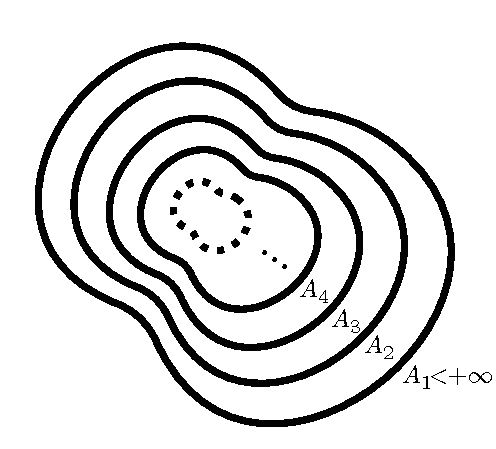
\includegraphics[trim=0cm 0cm 0cm 0cm, clip, scale=0.6]{images/misuracontinua2.pdf}
	\end{center}
	\end{itemize}
\end{property}
\begin{attention}
	Per la continuità da sopra è fondamentale l'ipotesi che $\mu\left(A_1\right)$ è finita.
\end{attention}
\begin{examplewt}[Controesempio alla continuità da sopra]
	Consideriamo la misura di Lebesgue unidimensionale $m_1$ e prendiamo la successione $A_n=\left[n,+\infty\right)$. Essa è decrescente in quanto
	\begin{equation*}
		A_{n+1}=\left[n+1,+\infty\right)\subsetneqq\left[n,+\infty\right)=A_n.
	\end{equation*}
	Si ha $m\left(A_n\right)=+\infty,\ \forall n$, e quindi in particolare
	\begin{equation*}
		\lim_{n\to+\infty}\mu\left(A_n\right)=+\infty
	\end{equation*}
	D'altro canto si ha
	\begin{equation*}
		\bigcap_{n\geq 1}A_n=\emptyset\implies\mu\left(\bigcap_{n\geq 1}A_n\right)=\mu\left(\emptyset\right)=0
	\end{equation*}
\end{examplewt}
\section{Famiglie di insiemi nella teoria della misura e relazioni tra di loro}\label{famigliediinsiemi}
Concludiamo questo capitolo alcune delle più comuni \textit{famiglie di insiemi} che si incontrano nello studio della teoria della misura.
\begin{center}
	\begin{tabular}{c|c|c}
		\textbf{Nome}                                                                            & \textbf{Notazione}                          & \textbf{Cardinalità}        \\ \hline
		Insieme delle parti                                                             & $\setpart{\realset}$               & $2^{\mathfrak{c}}$ \\ \hline
		\begin{tabular}[c]{@{}c@{}}Insiemi misurabili\\ (secondo Lebesgue)\end{tabular} & $\mathcal{L}\left(\realset\right)$ & $2^{\mathfrak{c}}$ \\ \hline
		Boreliani                                                                      & $\mathcal{B}\left(\realset\right)$ & $\mathfrak{c}$     \\ \hline
		\begin{tabular}[c]{@{}c@{}}Topologia\\ (famiglia degli aperti)\end{tabular}     & $\topo$                            & $\mathfrak{c}$    
	\end{tabular}
\end{center}
\begin{proposition}[Relazioni tra classi di insiemi]
	Valgono le seguenti inclusioni:
	\begin{equation}
		\topo\subsetneqq\mathcal{B}\left(\realset\right)\subsetneqq\mathcal{L}\left(\realset\right)\subsetneqq\setpart{\realset}
	\end{equation}
\end{proposition}
Mostreremo alcune di queste inclusioni in modo formale, mentre per altre daremo solo un'intuizione della dimostrazione.
\paragraph{Cardinalità dell'insieme delle parti dei reali}
Se $\abs{\realset}=\mathfrak{c}$ è la cardinalità del continuo, allora la cardinalità dell'\textit{insieme delle parti dei reali}\footnote{In ‘‘Brevi cenni di teoria degli insiemi'', a pag. \pageref{cardinalitàsetpart} è possibile trovare qualche dettaglio sulla cardinalità dell'insieme delle parti di un insieme e a pag. \pageref{cardinalitàsetpartreali} su quella dell'insieme delle parti dei reali.} è
\begin{equation}
	\abs{\setpart{\realset}}=2^{\mathfrak{c}}
\end{equation}
\paragraph{Cardinalità degli insiemi misurabili}
Per trovare quanti sono gli insiemi misurabili, consideriamo l'\textit{insieme di Cantor} $C$. Abbiamo visto\footnote{Si veda pag. \pageref{insiemecantor}.} che esso gode delle seguenti proprietà:
\begin{enumerate}
	\item Il numero di punti prima e dopo il processo iterativo per costruire $C$ rimane invariato, dunque $C$ è \textit{non numerabile} e ha la stessa cardinalità di $\left[0,1\right]$:
	\begin{equation*}
		\abs{C}=\abs{\left[0,1\right]}=\mathfrak{c}
	\end{equation*}
	\item $C$ è misurabile e $m_1\left(C\right)=0$.
\end{enumerate}
Dal punto 1 segue che l'insieme delle parti dell'insieme di Cantor ha cardinalità $\setpart{C}=2^{\mathfrak{c}}$, mentre dal punto 2 si può dedurre che ogni sottoinsieme di $C$ ha misura nulla ed è pertanto misurabile. Insiemisticamente parlando, le relazioni sono
\begin{equation*}
	\setpart{C}\subseteq \mathcal{L}\left(\realset\right)\subseteq\setpart{\realset}
\end{equation*}
Passando alle cardinalità:
\begin{equation*}
	2^{\mathfrak{c}}\underset{(1)}{=}{\abs{\setpart{C}}}\leq \abs{\mathcal{L}\left(\realset\right)}\leq\abs{\setpart{\realset}}=2^{\mathfrak{c}}\implies \abs{\mathcal{\realset}}=2^{\mathfrak{c}}
\end{equation*}
\paragraph{Inclusione stretta di {$\mathcal{L}\left(\realset\right)$} in {$\setpart{\realset}$}}
Il fatto che la cardinalità degli insiemi Lebesgue-misurabili in $\realset$ coincida con quella dell'insieme delle parti di $\realset$ non è sufficiente\footnote{Si veda ‘‘Brevi cenni di teoria degli insiemi'', pag. \pageref{cardinalitàugualenonimplicauguaglianzainsiemistica}.} per affermare che i due insiemi coincidano; costruiamo ora un sottoinsieme particolare di $\realset$ che risulta \textit{non misurabile}.
\begin{define}[Insieme di Vitali]\label{vitali}.
	Considerata in $\realset$ la relazione di equivalenza
	\begin{equation}
		x\sim y\iff x-y\in\rationalset
	\end{equation}
	possiamo definire delle classi di equivalenza in $\nicefrac{\realset}{\sim}$:
	\begin{align*}
		\left[0\right]&=\left\{0,1,\frac{1}{2},-\frac{3}{4},\frac{123}{72},\ldots\right\}=\left\{x\in\realset\mid x\in\rationalset\right\}=\rationalset\\
		\left[\sqrt{2}\right]&=\left\{\sqrt{2},\sqrt{2}+\frac{1}{2},\sqrt{2}-1,\ldots\right\}=\left\{x\in\realset\mid x=\sqrt{2}+q,\ q\in\rationalset\right\}\\
		\left[\pi\right]&=\left\{\pi,\pi-\frac{3}{4},\pi+23,\ldots\right\}=\left\{x\in\realset\mid x=\pi+q,\ q\in\rationalset\right\}\\
		\vdots
	\end{align*}
	Scelto\footnote{Per poter fare questa operazione è necessario supporre l'\textit{Assioma di Scelta}.} un elemento che stia in $\left[0,1\right]$ da ogni classe di equivalenza, definisco l'\textbf{insieme di Vitali}\index{insieme!di Vitali} $V$ come unione di questi elementi.
\end{define}
Per costruzione $V\subseteq\left[0,1\right]$. Preso l'insieme \textit{numerabile} $\rationalset\cap\left[0,1\right]$, possiamo prendere una sua \textit{numerazione} $\left\{q_n\right\}$ e definire delle \textit{traslazioni} dell'insieme di Vitali $V$:
\begin{equation*}
	V_n=V+q_n\subseteq\left[-1,2\right]
\end{equation*}
\begin{lemming}[Lemma 1 di Vitali - gli insiemi di Vitali traslati sono 2 a 2 disgiunti]
	Dato l'insieme di Vitali $V$  e una enumerazione $\left\{q_n\right\}$  di $\rationalset\cap\left[0,1\right]$, allora $V_n\cap V_m=\emptyset,\ \forall n\neq m$.
\end{lemming}
\begin{demonstration}
	Consideriamo $x\in V_n\cap V_m$: questo implica che $x\in V_n$ e $x\in V_m$, ossia
	\begin{equation*}
		\begin{cases}
			x=y+q_n,\ y\in V,\ q_n\in\rationalset\cap\left[-1,1\right]\\
			x=z+q_m,\ z\in V,\ q_m\in\rationalset\cap\left[-1,1\right]
		\end{cases}
	\end{equation*}
	Pertanto,
	\begin{equation*}
		y+q_n=z+q_m\iff y-z=q_m-q_n\in\rationalset
	\end{equation*}
	Poichè $y$ e $z$ differiscono di un razionale, essi appartengono alla stessa classe di equivalenza in $\nicefrac{\realset}{\sim}$, ma dato che nella costruzione dell'insieme di VItali abbiamo preso\footnote{In virtù dell'\textit{Assioma di Scelta}.} uno e un solo elemento da tale classe, allora segue che $y=z$. È immediato verificare che $q_m=q_n$ e, essendo elementi numerazione, allora $n=m$. In altre parole, l'intersezione non è vuota solo se $V_n=V_m$.
\end{demonstration}
\begin{lemming}[Lemma 2 di Vitali - ogni numero reale in {$\left[0,1\right]$} appartiene ad un $V_n$ per un certo $n$:]
	Dato l'insieme di Vitali $V$ vale la seguente relazione:
	\begin{equation*}
		\left[0,1\right]\subseteq\bigcup_{n\in\naturalset}V_n
	\end{equation*}
\end{lemming}
\begin{demonstration}
	Sia $x\in\left[0,1\right]$. Poiché la relazione $\sim$ forma una partizione di $\realset$, deve esistere $y$ tale che $x-y=q\in\rationalset$; riscrivendo tale relazione si ha $x=y+q$, ossia $x=y+q_n$ per un certo $n$.
\end{demonstration}
Possiamo osservare alcune proprietà sulla base dei due lemmi appena mostrati:
\begin{itemize}
	\item \textbf{Conseguenze del lemma 1:}
	\begin{equation*}
		m\left(\bigcup_{n\in\naturalset}V_n\right)=\sum_{n\in\naturalset}m\left(V_n\right)=\sum_{n\in\naturalset}m\left(V\right)=\begin{cases}
			\begin{array}{ll}
				0&\text{se }m\left(V\right)=0\\
				+\infty&\text{se }m\left(V\right)>0
			\end{array}
		\end{cases}
	\end{equation*}
	\item \textbf{Conseguenze del lemma 2:}
	\begin{equation*}
		1=m\left(\left[0,1\right]\right)\leq m\left(\bigcup_{n\in\naturalset}V_n\right)\leq m\left(\left[-1,2\right]\right)=3
	\end{equation*}
\end{itemize}
In altre parole, si deduce che
\begin{equation*}
	1\leq \sum_{n\in\naturalset}m\left(V\right)\leq 3
\end{equation*}
ma poiché la somma di infinite copie di $m\left(V\right)$ o è $0$ o è $+\infty$ per la conseguenza del lemma 1, in nessuno dei due casi la somma sta in $\left[1,3\right]$. Pertanto, $V$ \textit{non} è misurabile, in quanto non possiamo associargli un valore $m\left(V\right)$.
\paragraph{Cardinalità dei Boreliani e inclusione stretta di {$\mathcal{B}\left(\realset\right)$} in {$\mathcal{L}\left(\realset\right)$}}
Per \textit{induzione transfinita} si dimostra che i Boreliani hanno la cardinalità del continuo.
\begin{equation}
	\abs{\mathcal{B}\left(\realset\right)}=\abs{\realset}=\mathfrak{c}
\end{equation}
Pertanto, l'inclusione $\mathcal{B}\left(\realset\right)\subsetneqq \mathcal{L}\left(\realset\right)$ è stretta.\\
Dato che utilizziamo l'induzione transfinita su insiemi costruiti sui reali, è necessario usare l'Assioma della Scelta. Tuttavia, non è l'unico metodo per per dimostrare l'inclusione stretta di $\mathcal{B}\left(\realset\right)$ in $\mathcal{L}\left(\realset\right)$; infatti, si può costruire un insieme misurabile \textit{non} Boreliano senza fare uso dell'Assioma della Scelta. Per far ciò, definiamo prima la \textit{funzione di Cantor}.
\begin{define}[Funzione di Cantor]\label{funzionecantor}
	Si consideri l'insieme ternario di Cantor $C$. La \textbf{funzione di Cantor}\index{funzione!di Cantor} $\funz{c}{C}{C}$ è definita come
	\begin{equation}
		c(x) =\begin{cases} 
			\sum_{n=1}^\infty \frac{a_n}{2^n}, &\text{se } x = \sum_{n=1}^\infty 
			\frac{2a_n}{3^n}\in C\ \mathrm{dove}\ a_n\in\{0,1\}\\
			\sup_{y\leq x,\, y\in C} c(y), &\text{se } x\in [0,1]\setminus C.\\ \end{cases}
	\end{equation}
	Equivalentemente, preso $x\in\left[0,1\right]$ si può ottenere $c(x)$ con il seguente processo:
	\begin{itemize}
		\item Esprimi $x$ in base 3.
		\item Se $x$ contiene una cifra pari ad $1$, sostituire ogni cifra che segue il primo $1$ con $0$.
		\item Sostituire tutti i rimanenti $2$ con $1$.
		\item Interpretare il risultato come un numero binario, che diventerà $c(x)$.
	\end{itemize}
\end{define}
\begin{center}
	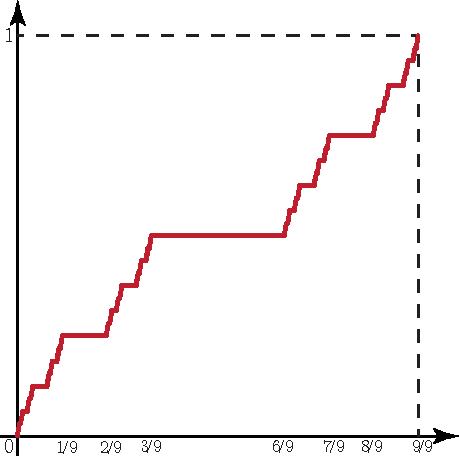
\includegraphics[width=0.4\paperwidth]{images/vasingolarecontinua}
\end{center}
Questa funzione non è altro che l'estensione della funzione $f$ incontrata nella dimostrazione dell'innumerabilità dell'insieme di Cantor ed è ben definita.\\
Si può dimostrare che $c$ è continua su $\left[0,1\right]$ ed è derivabile su $\left[0,1\right]\setminus C$ con
\begin{equation*}
	c'(x)=0,\ \forall x\in\realset\setminus C
\end{equation*}
Consideriamo ora la funzione $\funz{g}{\left[0,1\right]}{\left[0,1\right]}$ data da
\begin{equation}
	g(x)=\inf\left\{y\in\left[0,1\right]\mid c(y)=x\right\}
\end{equation}
Si ha che $g$ è una funzione iniettiva e monotona, dunque è misurabile e la controimmagine di un Boreliano tramite $g$ è ancora un Boreliano.\\
Consideriamo ora un insieme $E\subsetneqq \left[0,1\right]$ non misurabile secondo Lebesgue, dunque non è tanto meno un Boreliano. Si osservi che $F=g(E)\subseteq C$ è un insieme misurabile secondo Lebesgue perché la misura di Lebesgue è \textit{completa} ed è sottoinsieme di $C$, che ha misura nulla; tuttavia, $F$ non è un Boreliano, in quanto se lo fosse la controimmagine tramite $g$ dovrebbe essere un Boreliano, ma $g^{-1}(F)=E$, che non è però Boreliano!
%% SVN info for this file
\svnidlong
{$HeadURL$}
{$LastChangedDate$}
{$LastChangedRevision$}
{$LastChangedBy$}

\chapter{Integrale di Lebesgue}
\labelChapter{integraledilebesgue}

\begin{introduction}
	‘‘Si dovrebbe sempre generalizzare.''
	\begin{flushright}
		\textsc{Carl Jacobi,} prima che Teoria delle Categorie gli facesse cambiare idea.
	\end{flushright}
\end{introduction}
\lettrine[findent=1pt, nindent=0pt]{D}{opo} aver approfondito il tema della misura, in questo capitolo ci dedicheremo integralmente a parlare del punto focale del nostro studio, l'\textbf{integrale di Lebesgue}. La definizione che daremo \textit{non} è la stessa enunciata da Lebesgue, limitata alle funzioni \textit{da valori reali a valori reali}, bensì una generalizzazione avvenuta successivamente atta ad \textit{astrarre} (da qui il termine ‘‘astratto'') il concetto di integrale a funzioni da uno spazio di misura a valori reali (estesi) o complessi; per far ciò, sarà necessario definire l'integrale in tre passi consequenziali, estendendo gradualmente (ma con certe condizioni!) la famiglia di funzioni che ammettono integrale.
\section{I tre passi dell'integrale astratto di Lebesgue}
Primo di passare ad enunciare questi passi, premettiamo un paio di osservazioni su come questa definizione si distinguerà da quella dell'\textit{integrale di Riemann}:
\begin{enumerate}
	\item La definizione si dà per funzioni definite su uno spazio di misura $\left(X,\mathcal{M},\mu\right)$, mentre per Riemann le funzioni erano definite su $\realset$ o al più su $\realset^n$.	
	\item La definizione \textit{non} richiede alcuna ipotesi sulla misura di $X$, non distinguendo neanche casi tra misura finita e misura infinita.
\end{enumerate}
Come abbiamo annunciato, la definizione viene data per \textit{passaggi successivi}, utilizzando a partire dal passo 2 i passaggi precedenti. Supponiamo sempre di considerare funzioni con dominio un generico \textit{spazio di misura} $\left(X,\mathcal{M},\mu\right)$.
\begin{itemize}
	\item \textbf{\textsc{Passo 1:}} definiamo l'integrale per funzioni $\funz{s}{X}{\left[0,+\infty\right)}$ \textbf{semplici}, misurabili e non negative.
	\item \textbf{\textsc{Passo 2:}} definiamo l'integrale per funzioni
	$\funz{f}{X}{\left[0,+\infty\right]}$ \textbf{misurabili}, non negativi.
	\item \textbf{\textsc{Passo 3:}} definiamo l'integrale per funzioni $\funz{f}{X}{\complexset}$ \textbf{misurabili} e \textbf{integrabili}.
\end{itemize}
Prima di passare ai passi qui sopra enunciati, dobbiamo definire cos'è una \textit{funzione semplice} e capire come mai sono così importanti per l'integrale di Lebesgue.
\section{Funzioni semplici}
\begin{define}[Funzione semplice]
Una funzione $\funz{s}{\left(X,\mathcal{M}\right)}{\left[0,+\infty\right)}$, con $\left(X,\mathcal{M}\right)$ spazio misurabile, è detta \textbf{semplice}\index{funzione!semplice} se la sua immagine $S(X)$ è \textit{finita}.
\end{define}
Se $s$ ha l'immagine finita di cardinalità $n$, allora esistono $n$ valori distinti $\alpha_1,\ldots,\alpha_n$  valori \textit{distinti} tali che
\begin{equation*}
	s(x)=\left\{\alpha_1,\ldots,\alpha_n\right\}
\end{equation*}
Se consideriamo $A_i=\left\{x\mid s(x)=\alpha_i\right\}=s^{-1}\left(\left\{\alpha_i\right\}\right)$, allora possiamo decomporre $s$ come ‘‘somma pesata'' delle funzioni caratteristiche degli insiemi $A_i$ nella cosiddetta \textbf{decomposizione standard di }$s$\index{decomposizione standard di una funzione semplice}:
\begin{equation}
	s=\sum_{i=1}^{n}\alpha_i\chi_{A_i}
\end{equation}
\begin{proposition}[Una funzione semplice è misurabile se e solo se le controimmagini degli {$A_i$} sono misurabili]
	Una funzione semplice $s$, scritta in decomposizione standard come
	\begin{equation*}
		s=\sum_{i=1}^{n}\alpha_i\chi_{A_i}
	\end{equation*}
	è misurabile se e solo se gli insiemi $A_i=s^{-1}\left(\left\{\alpha_i\right\}\right)$ sono misurabili, $\forall i=1,\ \ldots,\ n$. 
\end{proposition}
\begin{demonstration}
	Per definizione di funzione misurabile,
	\begin{equation*}
		\funz{s}{\left(X,\mathcal{M}\right)}{\left[0,+\infty\right)}
	\end{equation*}
	è misurabile se e solo se $\forall A\subseteq\left[0,+\infty\right)$ aperto, la controimmagine
	\begin{equation*}
		s^{-1}\left(A\right)=\bigcup_{\alpha_i\in A}s^{-1}\left(\left\{\alpha_i\right\}\right)=\bigcup_{i\colon \alpha_i\in A}A_i
	\end{equation*}
è misurabile in $X$.\\
$\impliessx$ Poiché i valori $\alpha_i$, per definizione di $s$, sono finiti, per ogni $i$ possiamo considerare un intorno aperto $U\subseteq \left[0,+\infty\right)$ di $\alpha_i$ sufficientemente piccolo da non contenere alcun $a_j,\ \forall j\neq i$. Passando alla controimmagine
\begin{equation*}
	s^{-1}\left(U\right)=\bigcup_{k\colon \alpha_k\in U}A_k=A_i
\end{equation*}
per ipotesi sulla misurabilità di $s$ si ha che $A_i$ è misurabile, $\forall i$.\\
$\impliesdx$ Preso $A\subseteq\left[0,+\infty\right)$ aperto, abbiamo visto come la controimmagine è unione finita degli $A_i$:
	\begin{equation*}
	s^{-1}\left(A\right)=\bigcup_{i\colon \alpha_i\in A}A_i
\end{equation*}
Poiché per ipotesi gli $A_i$ sono misurabili, allora $A$ è unione di insiemi misurabili e quindi è anch'esso misurabile.
\end{demonstration}
\begin{examples}~{} \label{funzionesemplice}
	\begin{enumerate}
		\item Sia $\left(X,\mathcal{M}\right)=\left(\realset,\mathcal{L}(\realset)\right)$ e consideriamo la funzione $\funz{s}{\realset}{\realset}$ come da grafico.\\
		\begin{minipage}{0.4\textwidth}
			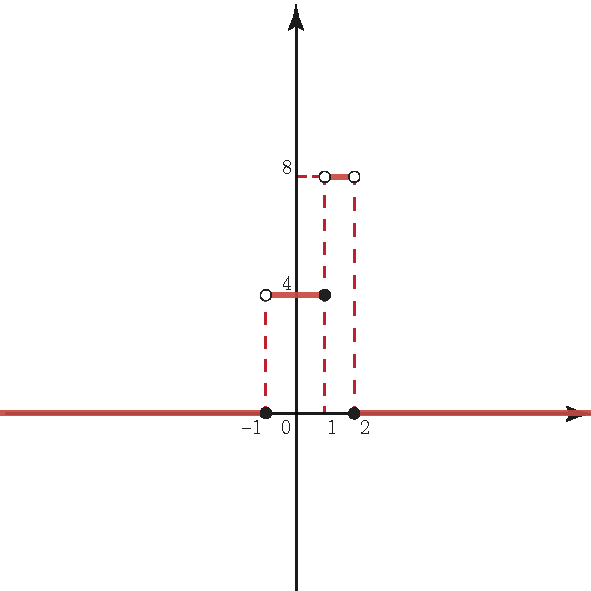
\includegraphics[trim=3cm 2cm 0cm 0cm, clip, scale=0.7]{images/graficosemplice.pdf}
		\end{minipage}\hspace{-7mm}
		\begin{minipage}{0.55\textwidth}
			Osserviamo che $s(X)=\left\{0,4,8\right\}$, dunque è semplice; le controimmagini dei valori $0$, $4$ e $8$ sono, rispettivamente:
			\begin{equation*}
				\begin{array}{l}
					A_1=s^{-1}\left(\left\{0\right\}\right)=\left(-\infty,-1\right]\cap\left[2,+\infty\right)\\
					A_2=s^{-1}\left(\left\{4\right\}\right)=\left(-1,1\right]\\
					A_3=s^{-1}\left(\left\{8\right\}\right)=\left(1,2\right)
				\end{array}
			\end{equation*}
		Pertanto la decomposizione standard di $s$ risulta
		\begin{align*}
			s&=0\chi_{\left(-\infty,-1\right]\cap\left[2,+\infty\right)}+4\chi_{\left(-1,1\right]}+8\chi_{\left(1,2\right)}=\\
			&=4\chi_{\left(-1,1\right]}+8\chi_{\left(1,2\right)}
		\end{align*}
		\end{minipage}\vspace{3mm}\\
	\item La funzione di Dirichlet
		\begin{equation*}
		s(x)=
		\begin{cases}
			\begin{array}{ll}
				1&\text{se }x\in\left[0,1\right]\cap\rationalset\\
				0&\text{se }x\in\left[0,1\right]\setminus\rationalset\\
			\end{array}
		\end{cases}
	\end{equation*}
	è semplice perché $s\left(\left[0,1\right]\right)=\left\{0,1\right\}$ e infatti $s=\chi_{\left[0,1\right]\cap\rationalset}$.
	\end{enumerate}
\end{examples}
\begin{minipage}{0.55\textwidth}
\subsection{Approssimazione di funzioni misurabili non negative con funzioni semplici}
Riprendendo l'idea di Lebesgue alla base del suo integrale, ci interessa studiare le funzioni passando attraverso la loro \textit{immagine}.\\
Si può ipotizzare di \textit{approssimare} tale funzione $f$ con una \textit{funzione semplice}: partizionando il codominio in opportuni intervalli individuati da quote fissate, se passiamo alle controimmagini possiamo sapere quali punti di $f$ sono contenuti nell'intervallo posto ad una certa quota e pertanto definire una funzione caratteristica che, come nelle \textit{carte topografiche a isoipse}, approssima la funzione $f$ per difetto.\\
Il prossimo teorema formalizza proprio questo ragionamento.
\end{minipage}\hspace{2mm}
\begin{minipage}{0.4\textwidth}
	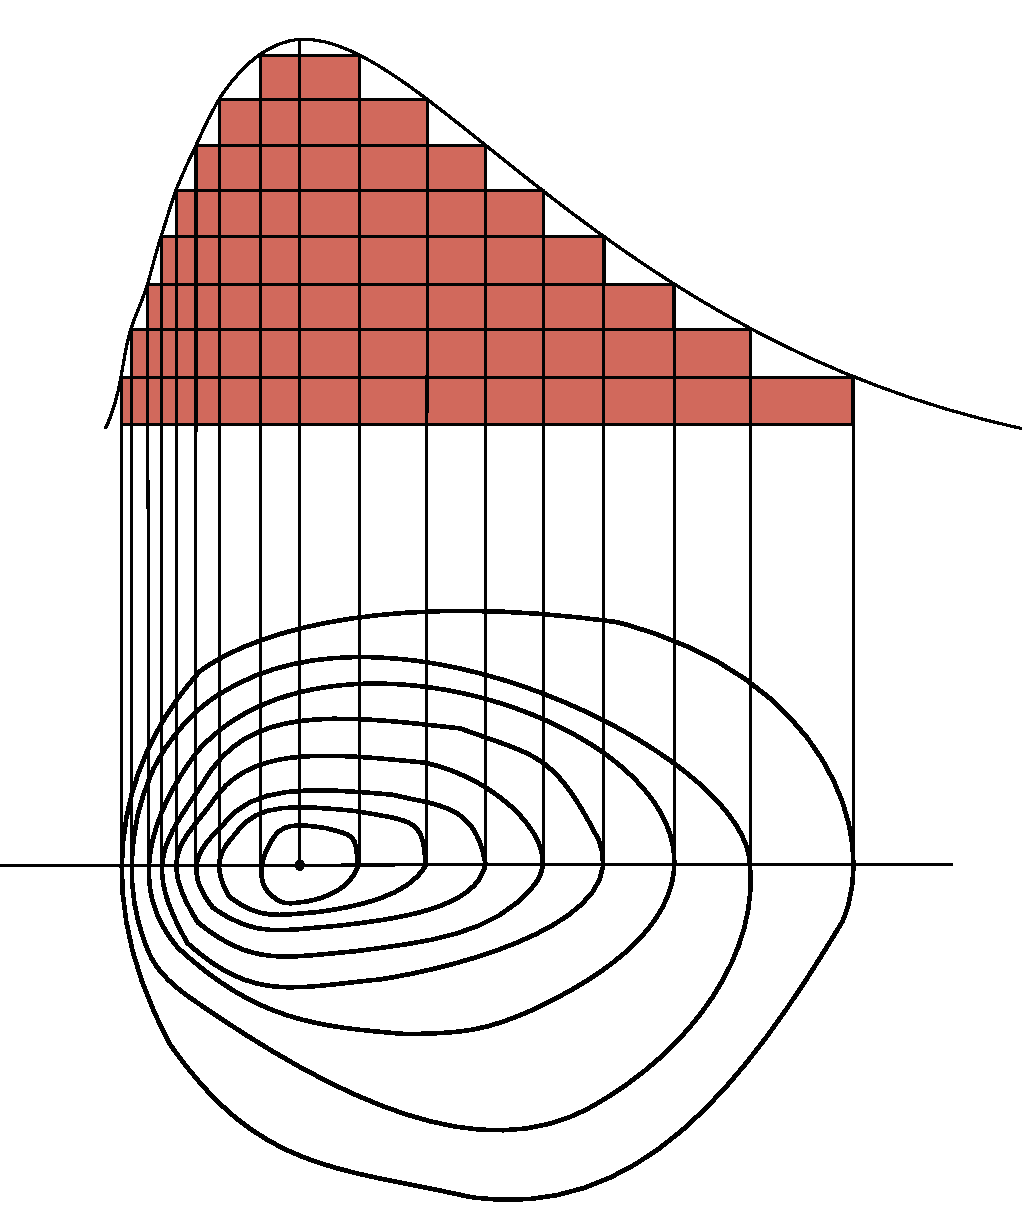
\includegraphics[trim=1cm 0cm 1.5cm 0cm, clip, scale=0.4]{images/isoipse}
\end{minipage}\vspace{3mm}\\
\begin{theorema}[Approssimazione di funzioni misurabili non negative con funzioni semplici]
	Sia $\left(X,\mathcal{M}\right)$ uno spazio misurabile e sia $\funz{f}{X}{\left[0,+\infty\right]}$ una funzione misurabile. Allora esiste una successione di funzioni semplici misurabili $\funz{s_n}{X}{\left[0,+\infty\right)}$ tale che
	\begin{itemize}
		\item $0\leq s_n(x)\leq s_{n+1}(x)\leq f(x),\ \forall x\in X,\ n\geq 1$.
		\item $\displaystyle\lim_{n\to+\infty}s_n(x)=f(x),\ \forall x\in X$.
	\end{itemize}
\end{theorema}
\begin{observe}
	La successione $s_n$ converge a $f$ puntualmente in modo \textit{monotono}.
\end{observe}
\begin{demonstration}~{}
	\begin{itemize}
		\item \textbf{\textsc{Passo 1}: costruzione della successione $s_n$ e verifica della monotonia.}\\
		Fissato $n\geq 1$, dividiamo $\left[0,+\infty\right)$ in $\left[0,n\right)$ e $\left[n,+\infty\right]$; dividiamo ulteriormente l'intervallo $\left[0,n\right)$ in $n2^n$ parti uguali
		\begin{equation*}
			\left[0,\frac{1}{2^n}\right)\quad\left[\frac{1}{2^n},\frac{2}{2^n}\right)\ldots\left[\frac{i-1}{2^n},\frac{i}{2^n}\right)\ldots\left[\frac{n2^n-1}{2^n},n\right),\ \forall i=1,\ \ldots,\ n2^n
		\end{equation*}
	Posto $E_{n,i}=f^{-1}\left(\left[\frac{i-1}{2^n},\frac{i}{2^n}\right)\right)$ e $F_n=f^{-1}\left(\left[n,+\infty\right]\right),\ \forall i=1,\ \ldots,\ n2^n$, si definisce
	\begin{equation}
		s_n=\sum_{i=1}^{n2^n}\frac{i-1}{2^n}\chi_{E_{n,i}}+n\chi_{F_n}
	\end{equation}
\begin{center}
	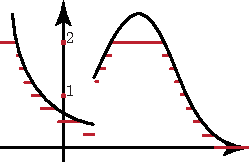
\includegraphics[trim=0cm 0cm 0cm 0cm, clip, scale=1.3]{images/approssimazione1}
\end{center}
Da questa costruzione segue che:
\begin{itemize}
	\item $s_n$ è semplice per $n$ fissato: è una combinazione lineare \textit{finita} di funzioni caratteristiche con pesi distinti.
	\item È monotona al crescere di $n$:\vspace{-3mm}
	\begin{equation*}
		0\leq s_n(x)\leq s_{n+1}(x)\leq f(x)\vspace{-3mm}
	\end{equation*}
	Intuitivamente, passando da $s_n$ a $s_{n+1}$:
	\begin{itemize}
		\item i nodi individuati in $s_n$ rimangono inalterati.
		\item vengono aggiunti dei nodi intermedi dimezzando ogni intervallino $\left[\frac{i-1}{2^n},\frac{i}{2^n}\right)$.
		\item vengono aggiunti dei nuovi nodi tra $n$ e $n+1$
	\end{itemize}
	Riducendo la dimensione di ciascun intervallino, l'approssimazione così definita risulta essere più raffinata del passo precedente; infatti, per ogni $x$ l'intervallo in cui sta ora $f(x)$ può avere lo stesso estremo inferiore che aveva con la partizione di $s_n$, oppure può avere un nuovo estremo inferiore dato da uno dei nodi introdotti con $s_{n+1}$.\\
\begin{minipage}{0.5\textwidth}
	\begin{center}
		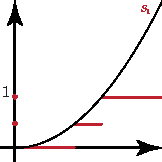
\includegraphics[trim=0cm 0cm 0cm 0cm, clip, scale=1.4]{images/approssimazione2}
	\end{center}
\end{minipage}
\begin{minipage}{0.5\textwidth}
	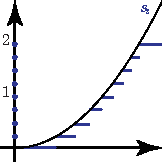
\includegraphics[trim=0cm 0cm 0cm 0cm, clip, scale=1.3]{images/approssimazione3}
\end{minipage}\vspace{4mm}
\end{itemize}
\item  \textbf{\textsc{Passo 2}: misurabilità di $s_n,\ \forall n\geq 1$.}\\
Ricordiamo che, dati $s_i\geq 0$ e $A_i\in\mathcal{M},\ i=1,\ \ldots,\ k$ si ha
\begin{equation*}
	s=\sum_{i=1}^{k}s_i\chi_{A_i}\text{ misurabile}\iff A_i\text{ misurabile},\ \forall i
\end{equation*}
Gli intervalli di $\left[\frac{i-1}{2^n},\frac{i}{2^n}\right),\ \forall i=1,\ \ldots,\ n2^n$ e $\left[n,+\infty\right)$ sono Boreliani in $\left[0,+\infty\right]$; pertanto, le controimmagini $E_{n,i}$ e $F_n$ tramite $f$ funzione misurabile sono anch'esse misurabili in $X$.
\item  \textbf{\textsc{Passo 3}: approssimazione nel senso della convergenza puntuale.}\\
	Proviamo che vale la relazione
	\begin{equation*}
		\lim_{n\to+\infty}s_n(x)=f(x),\ \forall x\in\ X
	\end{equation*}
Fissiamo $x\in X$ e distinguiamo i casi.
\begin{itemize}
	\item \textbf{\textsc{Caso 1:}} $f(x)\in\left[0,+\infty\right)$.\\
	Poiché $\floor{f(x)}\leq f(x)<\floor{f(x)}+1$, posto $N_x\coloneqq \floor{f(x)}+1$ si ha che
	\begin{equation*}
		f(x)< N_x\leq n,\ \forall n\geq N_x
	\end{equation*}
Pertanto, esiste $N_x\geq 1$ tale per cui $f(x)<n,\ \forall n\geq N_X$.\\
Sulla base di ciò si ha che $f(x)\in\left[0,n\right),\ \forall n\geq N_x$ e dunque esiste $i\in\left\{0,\ldots,n2^n\right\}$ tale per cui
\begin{equation*}
	f(x)\in\left[\frac{i-1}{2^n},\frac{i}{2^n}\right)\implies x\in f^{-1}\left(\left[\frac{i-1}{2^n},\frac{i}{2^n}\right]\right)=E_{n,i}
\end{equation*}
Allora $s_n(x)=\frac{i-1}{2^n}$ perché
\begin{gather*}
	\chi_{E_{n,j}}(x)=\delta_{i,j}\\
	\chi_{F_n}(x)\equiv 0
\end{gather*}
dove $\delta_{i,j}$ è il delta di Kronecker; segue che
\begin{equation*}
	0\leq s_n(x)=\frac{i-1}{2^n}\leq f(x)< \frac{i}{2^n}\implies 0\leq f(x)-s_n(x)<\frac{i}{2^n}
\end{equation*}
Passando al limite
\begin{equation*}
	0\leq \lim_{n\to+\infty}f(x)-s_n(x)\leq \lim_{n\to+\infty}\frac{i}{2^n}=0
\end{equation*}
Pertanto, per il \textit{teorema del confronto}
\begin{equation*}
	\lim_{n\to+\infty}f(x)-s_n(x)=0\implies \lim_{n\to+\infty}s_n(x)=f(x).
\end{equation*}
\item \textbf{\textsc{Caso 2:}} $f(x)=+\infty$.\\
Chiaramente
\begin{equation*}
	f(x)\in\left[n,+\infty\right],\ \forall n\geq 1\implies x\in f^{-1}\left(\left[n,+\infty\right]\right)=F_n
\end{equation*}
Allora $s_n(x)=n$ perché
\begin{gather*}
	\chi_{E_{n,j}}(x)\equiv 0\\
	\chi_{F_n}(x)\equiv 1
\end{gather*}
Segue che
\begin{equation*}
	\lim_{n\to+\infty}s_n(x)=\lim_{n\to+\infty}n=+\infty=f(x)\implies \lim_{n\to+\infty}s_n(x)=f(x)\qedhere
\end{equation*}
\end{itemize}
\end{itemize}
\end{demonstration}

\section{Passo 1: funzioni semplici, misurabili, non negative}
\begin{define}[Integrale di Lebesgue per funzioni semplici, misurabili, non negative]
	Sia $\funz{s}{\left(X,\mathcal{M},\mu\right)}{\left[0,+\infty\right)}$ funzione semplice, misurabile e non negativa che si decompone, dato $s(X)=\left\{\alpha_1,\ldots, \alpha_n\right\}$, nella forma standard
	\begin{equation*}
		s=\sum_{i=1}^{n}\alpha_i\chi_{A_i}\quad A_i=s^{-1}\left(\left\{A_i\right\}\right)
	\end{equation*}
	Dato $E\in\mathcal{M}$, si definisce \textit{integrale esteso a $A$ di $s$ rispetto alla misura $\mu$} il valore
	\begin{equation}
		\int_{E}sd\mu\coloneqq\sum_{i=1}^{n}\alpha_i\mu\left(A_i\cap E\right)
	\end{equation}
	con la convenzione che se un termine di tale sommatoria è $0\cdot \infty$ allora tale termine sia uguale a $0$.
\end{define}
\begin{observe}
	$\mu\left(A_i\cap E\right)$ è ben definito in quanto $A_i\cap E$ è misurabile:
	\begin{itemize}
		\item $A_i$ sono misurabili $\forall i$ perché $s$ è misurabile per ipotesi.
		\item $E$ è misurabile per ipotesi.
		\item L'\textit{intersezione} è un'operazione chiusa nella $\sigma$-algebra $\mathcal{M}$
	\end{itemize}
\end{observe}
\begin{observe}
	Come mai poniamo convenzionalmente $0\cdot \infty=0$? L'integrale generalizza e astrae il calcolo dell'area sottesa ad una curva; se ho un intervallo di lunghezza infinita ma a quota zero, chiaramente l'area sottesa è uguale a zero.
\end{observe}
\begin{examples} Per il primo e secondo esempio riprendiamo le funzioni viste a pag. \pageref{funzionesemplice}.
	\begin{enumerate}
		\item Consideriamo la funzione del primo esempio, che ha dominio in $\left(\realset^n,\mathcal{L}(\realset),m_1\right)$ e calcoliamo l'integrale su $E=\realset$:
		\begin{equation*}
			\begin{array}{ll}
				\displaystyle	\int_{\realset}sdm_1&=0m_1\left(\left(-\infty,-1\right]\cup\left[2,+\infty\right)\right)+4m_1\left(\left[-1,1\right]\right)+8m_2\left(\left(1,2\right)\right)=\\
				&=0\cdot\left(+\infty\right)+4\cdot 2+8\cdot 1=16
			\end{array}
		\end{equation*}
		\item \label{funzionedirichletintegrale}Consideriamo la funzione di Dirichlet su $\left[0,1\right]$, che ha dominio in $\left(\realset,\mathcal{L}(\realset),m_1\right)$  l'integrale su $E=\left[0,1\right]$:
		\begin{equation*}
			\int_{\left[0,1\right]}sdm_1=1\cdot m_1\left(\left[0,1\right]\cap\rationalset\right)+0\cdot m_1\left(\left[0,1\right]\setminus\rationalset\right)
		\end{equation*}
	Poiché
	\begin{itemize}
		\item $\left[0,1\right]\cap \rationalset$ è misurabile e si ha $m_1\left(\left[0,1\right]\cap \rationalset\right)=0$.
		\item $m_1\left(\left[0,1\right]\setminus\rationalset\right)=m1\left(\left[0,1\right]\right)-m1\left(\left[0,1\right]\cap\rationalset\right)=1-0=1$
	\end{itemize}
	allora
	\begin{equation*}
		\int_{\left[0,1\right]}sdm_1=1\cdot 0+0\cdot 1=0
	\end{equation*}
\item Consideriamo $\left(X,\mathcal{M},\mu\right)=\left(\naturalset,\setpart{\naturalset},\mu_p\right)$ con $\mu_p$ la misura di conteggio di \textbf{Poisson} di parametro $\lambda>0$:\index{misura!di conteggio!di Poisson}.
\begin{gather}
	\mu_p\left(\left\{n\right\}\right)=e^{-\lambda}\frac{\lambda^n}{n!}, \forall n\geq 0\\
	\mu_p\left(E\right)=\sum-{n\colon n\in E}e^{-\lambda}\frac{\lambda^n}{n!}, \forall E\subseteq \naturalset
\end{gather}
Definiamo $\funz{s}{\naturalset}{\left[0,+\infty\right)}$ come
\begin{equation*}
	s\left(n\right)=\begin{cases}
		\begin{array}{ll}
			1&\text{se }n=0,1\\
			2&\text{se }n\geq 2
		\end{array}
	\end{cases}
\end{equation*}
La funzione $s$ è semplice, dato che $s\left(\naturalset\right)=\left\{1,2\right\}$, e
\begin{equation*}
	s=\chi_{\left\{0,1\right\}}+2\chi_{\left\{n\in\naturalset\mid n\geq 2\right\}}
\end{equation*}
Allora, posto $E=\naturalset$, l'integrale sul dominio è
\begin{equation*}
\begin{array}{ll}
	\displaystyle\int_{\naturalset}sd\mu_P&=1\cdot \mu_P\left(\left\{0,1\right\}\right)+2\mu_P\left(\left\{n\in\naturalset\mid n\geq 2\right\}\right)=\\
	&\displaystyle=e^{-\lambda}\cdot 1+e^{-\lambda}\frac{\lambda}{1}+2\sum_{n\geq 2}e^{-\lambda}\frac{\lambda^n}{n!}=\\
	&\displaystyle=e^{-\lambda}+\lambda e^{-\lambda}+2\sum_{n\geq 2}e^{-\lambda}\frac{\lambda^n}{n!}
\end{array}
\end{equation*}
	\end{enumerate}
\end{examples}
\begin{observe}
	La funzione di Dirichlet è una funzione \textit{non} integrabile secondo \textit{Riemann}, ma è integrabile secondo Lebesgue.
\end{observe}
\subsection{{$\sigma$}-additività dell'integrale di funzioni semplici, misurabili, non negative rispetto al dominio}
\begin{proposition}[{$\sigma$}-additività dell'integrale di funzioni semplici, misurabili, non negative rispetto al dominio]
	Sia $\left(X,\mathcal{M},\mu\right)$ uno spazio di misura e sia $\funz{s}{X}{\left[0,+\infty\right)}$ semplice misurabile \textit{non} negativa. Allora vale
	\begin{equation}
		\int_{\union_{n\geq 1}E_n}sd\mu=\sum_{n\geq 1}\int_{E_n}sd\mu,\ \forall E_n\in\mathcal{M}\colon E_i\cap E_j=\emptyset,\ \forall i\neq j
	\end{equation}
\end{proposition}
Per dimostrare tale proprietà ci servirà un risultato sulle serie con \textit{doppi indici}.
\begin{propositionsqed}[Commutatività degli indici nelle serie doppie]~\label{commutativitàindici}
	\begin{itemize}
		\item Se $a_{ij}\geq0\ \forall i,j$, allora
		\begin{equation*}
			\sum_{i=1}^{+\infty}\sum_{j=1}^{+\infty}a_{ij}=\sum_{j=1}^{+\infty}\sum_{i=1}^{+\infty}a_{ij}
		\end{equation*}
		\item Più in generale, se $\displaystyle\sum_{i=1}^{+\infty}\sum_{j=1}^{+\infty}\abs{a_{ij}}<+\infty$, allora vale la relazione precedente.\qedhere
	\end{itemize}
\end{propositionsqed}
\begin{demonstrationwt}[della {$\sigma$}-additività dell'integrale rispetto al dominio]
	Siano $E_n\in\mathcal{M},\ E_i\cap E_j= \emptyset$ e sia $\displaystyle E=\cup_{n\geq 1} E_n$. Sia $\displaystyle s=\sum_{i=1}^{k}\alpha_i\chi_{A_i}$ la decomposizione standard di $s$ funzione semplice, dove $s(x)=\left\{\alpha_1,\ldots,\alpha_k\right\}$ e $A_i=s^{-1}\left(\left\{\alpha_i\right\}\right),\ \forall i=1,\ \ldots,\ k$. Si ha
	\begin{equation*}
		\int_Esd\mu=\sum_{i=1}^{k}\alpha_i\mu\left(A_i\cap E\right)\squarequal
	\end{equation*}
	Per $\sigma$-additività della misura $\mu$ vale
	\begin{equation*}
		\mu\left(A_i\cap E\right)=\sum_{j=1}^{+\infty}\mu\left(A\cap E_j\right)
	\end{equation*}
quindi
\begin{equation*}
	\squarequal \sum_{i=1}^{k}\alpha_i\sum_{j=1}^{+\infty}\mu\left(A_i\cap E_j\right)=\sum_{i=1}^{k}\sum_{j=1}^{+\infty}\underbrace{\alpha_i\mu\left(A_i\cap E_j\right)}_{\geq 0}=\sum_{j=1}^{+\infty}\sum_{i=1}^{k}\alpha_i\mu\left(A_i\cap E_j\right)=\sum_{j=1}^{+\infty}\int_{E_j}sd\mu
\end{equation*}
\end{demonstrationwt}
Vediamo il risultato appena dimostrato da un punto di vista differente. Possiamo considerare l'integrale di Lebesgue non solo come un \textit{funzionale} che, fissato un insieme misurabile $E\in\left(X,\mathcal{M},\mu\right)$, agisce sulla funzione $s$, bensì come una \textit{funzione d'insieme} in cui $s$ è fissata, mentre la variabile è l'insieme misurabile $E$:
\begin{equation}
	\funztot{\mu_s}{\mathcal{M}}{\left[0,+\infty\right]}{E}{\int_Esd\mu}
\end{equation}
L'uguaglianza ricavata dalla proposizione precedente 
\begin{equation*}
	\int_{\cup_{n\geq 1}E_n}sd\mu=\sum_{n\geq 1}\int_{E}sd\mu,\ \forall E_n\in\mathcal{M}\colon E_i\cap E_j=\emptyset,\ \forall i\neq j
\end{equation*}
si riscrive pertanto come
\begin{equation*}
	\mu_s\left(\bigcup_{n\geq 1}E_n\right)=\sum_{n\geq 1}\mu_s\left(E_n\right)
\end{equation*}
Pertanto, $\mu_s$ è una misura su $\mathcal{M}$.
\section{Passo 2: funzioni a valori reali misurabili, non negative}
Sia $\funz{f}{\left(X,\mathcal{M},\mu\right)}{\left[0,+\infty\right]}$ funzione misurabile e non negativa. Dato $E\in\mathcal{M}$, vogliamo definire l'\textit{integrale esteso ad E di $f$ rispetto alla misura $\mu$} utilizzando l'integrale delle funzioni semplici definito al passo 1. 
\begin{define}[Integrale di Lebesgue per funzioni a valori reali, misurabili, non negative]
	Sia $\funz{f}{\left(X,\mathcal{M},\mu\right)}{\left[0,+\infty\right]}$ funzione misurabile e non negativa. Si definisce l'\textit{integrale esteso ad E di $f$ rispetto alla misura $\mu$} come
	\begin{equation}
		\int_Efd\mu\coloneqq\sup\left\{\int_Esd\mu\ \middle| \funz{s}{X}{\left[0,+\infty\right)}\text{ semplice, misurabile}\colon0\leq s\leq f\right\}
	\end{equation}
\end{define}
\begin{observe}~{}
	\begin{itemize}
		\item L'insieme
		\begin{equation*}
			\left\{\int_Esd\mu\ \middle|\funz{s}{X}{\left[0,+\infty\right)}\text{ semplice, misurabile}\colon0\leq s\leq f\right\}\subseteq \left[0,+\infty\right]
		\end{equation*} non è vuoto, in quanto contiene sempre $0=\int_E 0d\mu$.
		\item $\int_Efd\mu\in\left[0,+\infty\right]$
		\item Se $f$ è semplice allora si ritrova l'integrale definito al \textit{passo 1}.
	\end{itemize}
\end{observe}
\begin{attention}~{}\\
	\textbf{Ogni funzione misurabile \textit{non negativa} ammette integrale secondo Lebesgue.}\\
	Questa notevole differenza rispetto all'integrale di Riemann è situa nella definizione. Se l'integrale di Riemann richiede che la somma inferiore e la somma superiore coincidono, quello di Lebesgue richiede solo l'esistenza del $\sup$: la prima condizione non si verifica sempre, mentre la seconda è sempre verificata in $\realset^{\ast}$.
\end{attention}
\begin{property}[Proprietà dell'integrale di Lebesgue per funzioni misurabili non negative]
	Sia $\left(X,\mathcal{M},\mu\right)$ uno spazio di misura.
	\begin{enumerate}
		\item \textbf{Monotonia rispetto alla funzione integranda:}\\
		date $\funz{f,g}{X}{\left[0,+\infty\right]}$ misurabili, non negative tali per cui $f\leq g$, allora
		\begin{equation}
			\int_E fd\mu\leq \int_E gd\mu,\ \forall E\in\mathcal{M}
		\end{equation}
		\item \textbf{Monotonia rispetto al dominio della funzione integranda:}\\
		dati $\funz{f}{X}{\left[0,+\infty\right]}$ misurabile, non negativa e $E,\ F\in\mathcal{M}$ tali per cui $E\subseteq F$, allora
		\begin{equation}
			\int_Efd\mu\leq \int_Fgd\mu
		\end{equation}
		\item \textbf{Linearità dell'integrale (prodotto per uno scalare):}\\
		dati $\funz{f}{X}{\left[0,+\infty\right]}$ misurabile, non negativa e $c\geq 0$
		\begin{equation}
			\int_E cfd\mu=c\int_Efd\mu,\ \forall E\in\mathcal{M}
		\end{equation}
		\item \textbf{Ininfluenza degli insiemi di misura nulla sull'integrale:}\\
		sia $\funz{f}{X}{\left[0,+\infty\right]}$ misurabile, non negativa; se $E\in\mathcal{M}$ con $\mu\left(E\right)=0$, allora
		\begin{equation}
			\int_Efd\mu=0
		\end{equation}
		\item \textbf{Integrazione sullo spazio intero:}\\
		sia $\funz{f}{X}{\left[0,+\infty\right]}$ misurabile, non negativa; allora
		\begin{equation}
			\int_E fd\mu=c\int_Xf\chi_Ed\mu,\ \forall E\in\mathcal{M}
		\end{equation}
	\end{enumerate}
\end{property}
\subsection{Teorema della convergenza monotona}
Il \textbf{teorema della convergenza monotona}\index{teorema!della convergenza monotona}, altresì noto come \textbf{Teorema di Beppo Levi}\seeonlyindex{teorema!di Beppo Levi}{teorema!della convergenza monotona} (principalmente in Italia) o di \textbf{Lebesgue}\seeonlyindex{teorema!di Lebesgue}{teorema!della convergenza monotona}, si inserisce nel filone dei risultati sul problema del \textit{passaggio al limite sotto segno di integrale} di cui abbiamo parlato per la prima volta nel \refChapterOnly{ellipseintroduction}.\\
Abbiamo già visto\footnote{Si veda \refChapterOnly{seriefunzioni}, teorema \ref{passaggioallimitecontinuitàuniforme}, pag. \pageref{passaggioallimitecontinuitàuniforme}.} che se una successione di funzioni $f_n$ Riemann-integrabili su un compatto converge uniformemente a $f$, allora $f$ è Riemann-integrabile e vale il passaggio al limite dell'integrale. Il teorema che dimostreremo, pur essendo applicabile solo a funzioni misurabili e monotone \textit{crescenti}, risulta avere diversi notevoli vantaggi rispetto al risultato basato sulla convergenza uniforme.
\begin{theorema}[Teorema della convergenza monotona]\label{thmconvergenzamonotona}
	Siano $\left(X,\mathcal{M},\mu\right)$ uno spazio di misura e $\funz{f_n,f}{X}{\left[0,+\infty\right]}$ con $n\geq 1$ tali che
	\begin{enumerate}[label=(\alph*)]
		\item $f_n$ sono misurabili.
		\item $\displaystyle\lim_{n\to+\infty}f_n(x)=f(x),\ \forall x\in X$.
		\item $0\leq f_n(x)\leq f_{n+1}(x),\ \forall n\geq 1,\ \forall x\in X$.
	\end{enumerate}
Allora
\begin{enumerate}
	\item $f$ è misurabile.
	\item Vale il \textbf{passaggio al limite sotto segno di integrale}\index{passaggio al limite sotto segno di integrale}:
	\begin{equation}
		\lim_{n\to+\infty}\int_Xf_nd\mu=\int_Xfd\mu\in\left[0,+\infty\right]
	\end{equation}
\end{enumerate}
\end{theorema}
\begin{observes}~{}
	\begin{itemize}
		\item L'uguaglianza della tesi è valida per ogni misura di $X$, anche infinita.
		\item Il risultato è in generale \textit{falso} se $f_n(x)$ decresce rispetto ad $n,\ \forall x\in X$.
	\end{itemize}
\end{observes}
\begin{examplewt}[Controesempio con una successione di funzioni decrescenti]
	Sia $\left(X,\mathcal{M},\mu\right)=\left(\realset,\mathcal{L}(\realset),m_1\right)$ e $f_n(x)=\frac{1}{n},\ \forall x\in\realset$. Per ogni $x$ vale
	\begin{itemize}
		\item $f_n(x)$ decrescente rispetto ad $n$.
		\item $\displaystyle\lim_{n\to+\infty}f_n(x)=0$
	\end{itemize}
Pertanto:
\begin{align*}
	\lim_{n\to+\infty}\int_{\realset}f_ndm_1=\lim_{n\to+\infty}\left(+\infty\right)&=+\infty\\
	\int_{\realset}\left(\lim_{n\to+\infty}f_n\right)dm_1=\int_{\realset}0dm_1&=0
\end{align*}
\end{examplewt}
\begin{demonstrationcaputwt}[del teorema della convergenza monotona]~
	\begin{enumerate}[label=\Roman*]
		\item $f$ è misurabile perché è limite puntuale di funzioni misurabili.
		\item Osserviamo che $f$ misurabile e non negativa implica che
		\begin{equation*}
			\exists\int_Xfd\mu\in\left[0,+\infty\right]
		\end{equation*}
		Dalla monotonia data per ipotesi c) segue, per monotonia dell'integrale rispetto alla funzione integranda, che
	\begin{equation*}
		0\leq\lefteqn{\underbrace{\phantom{\int_Xf_nd\mu\leq\int_Xf_{n+1}d\mu}}_{\circled[red]{\vardiamond}}}\int_Xf_nd\mu\leq
		\overbrace{\int_Xf_{n+1}d\mu\leq \int_Xfd\mu}^{\circled[blue]{\spadesuit}}
	\end{equation*}
		Da \circled[red]{\vardiamond} si nota come la successione
	\begin{equation*}
		\int_Xf_nd\mu\in\left[0,+\infty\right]
	\end{equation*}
		è crescente e quindi per il \textit{teorema sui limiti di successioni monotone} esiste il suo limite
\begin{equation*}
	\lim_{n\to+\infty}\int_Xf_nd\mu\in\left[0,+\infty\right]
\end{equation*}
Considerando \circled[blue]{\spadesuit}, per il \textit{teorema della permanenza del segno} si ottiene
\begin{equation*}
	\lim_{n\to+\infty}\int_Xf_nd\mu\leq \int_Xfd\mu
\end{equation*}
È sufficiente dimostrare che vale la disuguaglianza di verso opposto:
\begin{equation*}
	\lim_{n\to+\infty}\int_Xf_nd\mu\geq \int_Xfd\mu
\end{equation*}
Ricordiamo che per definizione
\begin{equation*}
	\int_Xfd\mu=\sup\left\{\int_Xsd\mu\middle| \funz{s}{X}{\left[0,+\infty\right)}\text{ semplice, misurabile}\colon0\leq s\leq f\right\}
\end{equation*}
Pertanto ci sarà sufficiente provare che
\begin{equation*}
	\lim_{n\to+\infty}\int_Xf_nd\mu\geq \int_Xsd\mu,\ \forall s\text{ funzione definita come sopra.}
\end{equation*}
Osserviamo che questa è vera se mostriamo che
\begin{equation*}
	\lim_{n\to+\infty}\int_Xf_nd\mu\geq c\int_Xsd\mu,\ \forall s\text{ funzione definita come sopra},\ \forall c\in\left(0,1\right)
\end{equation*}
Basterà infatti passare poi al limite per $c\to 1^{-}$ per ottenere la condizione cercata.\\
Siano quindi $c\in\left(0,1\right)$ e $\funz{s}{X}{\left[0,+\infty\right]}$ semplice, misurabile e tale che $0\leq s\leq f$ su $X$. Per ogni $n\geq 1$ definiamo
\begin{equation*}
	E_n=\left\{x\in X\mid f_n(x)\geq cs(x)\right\}
\end{equation*}
Osserviamo che se $x\in\ E_n$, allora
\begin{equation*}
	f_n(x)\geq cs(x)\implies f_{n+1}(x)\geq f_n(x)\geq cs(x)\implies x\in E_{n+1},\ \forall n\geq 1,
\end{equation*}
cioè $E_n\subseteq E_{n+1},\ \forall n\geq 1$.
Ora abbiamo
\begin{equation*}
	\int_Xf_nd\mu\geq \int_{E_n}f_nd\mu\geq \int_{E_n}csd\mu=c\int_Esd\mu=c\mu_s\left(E_n\right)
\end{equation*}
dove $\mu_s$ è la misura definita come 
\begin{equation*}
	\mu_s\left(E\right)=\int_Esd\mu
\end{equation*}
Abbiamo quindi ricavato che
\begin{equation*}
	\circled[green]{\clubsuit}\int_Xf_nd\mu\geq c\mu_s\left(E_n\right),\ \forall n\geq 1
\end{equation*}
Se $n\to+\infty$, essendo $\mu_S$ una misura $E_n$ una successione insiemistica crescente, per continuità della misura
\begin{equation*}
	\lim_{n\to+\infty}\mu_s\left(E_n\right)=\mu_s\left(\bigcup_{n\geq 1}E_n\right)
\end{equation*}
Passando al limite nella disequazione \circled[green]{\clubsuit} otteniamo
\begin{equation*}
	\lim_{n\to+\infty}\int_Xf_nd\mu\geq c\mu_s\left(\bigcup_{n\geq 1}E_n\right)=c\int_{\bigcup_{n\geq 1}E_n}d\mu_s
\end{equation*}
Per concludere, proviamo che
\begin{equation*}
	\bigcup_{n\geq 1}E_n=X
\end{equation*}
Banalmente l'inclusione $\subseteq$ è verificata; per trovare l'altra si usa la convergenza puntuale di $f_n(x)$ e $f(x),\ \forall x\in X$. Poiché $f_n$ è una successione di funzioni crescenti e con limite puntuale a $f$ su $X$, sappiamo che $f_n\leq f$ e quindi
\begin{equation*}
	f(x)\geq f_n(x)\geq cs(x)
\end{equation*}
Prendiamo ora $x\in X$: se $f(x)=0$, allora $x\in E_1$ in quanto segue che $s(x)=0$; se $f(x)>0$, allora $x\in E_n$ per qualche $n$.
\qedhere
\end{enumerate}
\end{demonstrationcaputwt}
\subsection{Additività dell'intergrale, scambio di integrale e serie}
\begin{proposition}[Additività dell'integrale]
	Sia $\left(X,\mathcal{M},\mu\right)$ uno spazio di misura e siano $\funz{f_1,\ \ldots,\ f_N}{X}{\left[0,+\infty\right]}$ funzioni misurabili. Allora
	\begin{equation}
		\int_X \left(\sum_{i=1}^{N}f_i\right)d\mu=\sum_{i=1}^{N}\int_Xf_id\mu
	\end{equation}
\end{proposition}
\begin{observe}
	\textit{Tutti} gli integrali nell'enunciato esistono (eventualmente infiniti) in quanto le $f_i$ sono funzioni misurabili non negative.
\end{observe}
\begin{demonstration}
	Si prova per induzione su $N$. Il passo induttivo è immediato, pertanto proviamo la base dell'induzione ($N=2$): dimostriamo dunque che
	\begin{equation*}
		\int_X\left(f_1+f_2\right)d\mu=\int_Xf_1d\mu+\int_Xf_2d\mu
	\end{equation*}
		\begin{itemize}
		\item \textbf{\textsc{Passo 1}:} proviamo il risultato nel caso di funzioni semplici $\funz{s,t}{X}{\left[0,+\infty\right)}$ misurabili. Esse si possono scrivere come
		\begin{equation*}
			\begin{array}{lll}
				& \displaystyle s=\sum_{i=1}^{k}s_i\chi_{A_i} & \displaystyle t=\sum_{i=1}^n{k}t_j\chi_{B_j}\\
				\text{dove}& \displaystyle s(x)=\left\{s_1,\ldots,s_k\right\}&\displaystyle t(x)=\left\{t_1,\ldots,t_n\right\}\\
				&\displaystyle A_i=s^{-1}\left(\left\{s_i\right\}\right),\ i=1,\ldots,\ k&\displaystyle B_j=t^{-1}\left(\left\{t_j\right\}\right),\ j=1,\ldots,\ n\\
			\end{array}
		\end{equation*}
	Consideriamo $E_{i,j}=A_i\cap B_j,\ \forall i,\ \ldots,\ k$ e $j=1,\ \ldots,\ n$: essi formano una nuova partizione di $X$ e, preso $x\in E_{ij}$, si ha
	\begin{equation*}
		\begin{cases}
			s(x)=s_i\\
			t(x)=t_j
		\end{cases}
	\end{equation*}
\begin{center}
	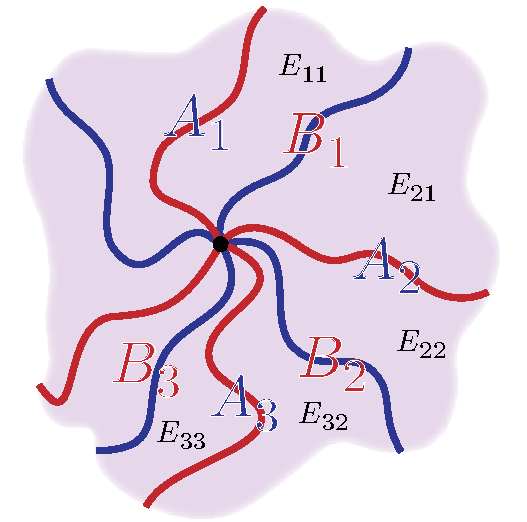
\includegraphics[trim=0cm 0cm 0cm 0cm, clip, scale=0.75]{images/additivita}
\end{center}
	Questo significa che $s(x)+t(x)=s_i+t_j,\ \forall x\in E_{ij}$, ossia
	\begin{equation*}
		s+t=\sum_{i,j}\left(s_i+t_j\right)\chi_{E_{ij}}
	\end{equation*}
	Integriamo secondo Lebesgue:
	\begin{equation*}
		\int_X\left(s+t\right)d\mu=\sum_{i,j}\left(s_i+t_j\right)\mu\left(E_{ij}\right)=\sum_{i,j}s_i\mu\left(E_{ij}\right)+\sum_{i,j}t_j\mu\left(E_{ij}\right)=\int_Xsd\mu+\int_Xtd\mu
	\end{equation*}
	\item \textbf{\textsc{Passo 2}:} proviamo il risultato nel caso di funzioni $\funz{f_1,f_2}{X}{\left[0,+\infty\right)}$ misurabili.\\
	È noto che:
	\begin{itemize}
		\item Esiste una successione di funzioni semplici misurabili $\funz{s_n}{X}{\left[0,+\infty\right]}$ tali che
		\begin{itemize}
			\item $0\leq s_n(x)\leq s_{n+1}(x)\leq f_1(x),\ \forall x\in X$.
			\item $\displaystyle \lim_{n\to+\infty}s_n(x)=f_1(x),\ \forall x\in\ X$
		\end{itemize}
		\item Esiste una successione di funzioni semplici misurabili $\funz{t_n}{X}{\left[0,+\infty\right]}$ tali che
		\begin{itemize}
			\item $0\leq t_n(x)\leq t_{n+1}(x)\leq f_2(x),\ \forall x\in X$.
			\item $\displaystyle \lim_{n\to+\infty}t_n(x)=f_2(x),\ \forall x\in\ X$
		\end{itemize}
	\end{itemize}
	Di conseguenza si ha
	\begin{align*}
		0\leq \left(s_n+t_n\right)(x)\leq \left(s_{n+1}+t_{n+1}\right)(x)\leq\left(f_1+f_2\right)(x),\ \forall x\in\ X\\
		\lim_{n\to+\infty}\left(s_n+t_n\right)(x)=\left(f_1+f_2\right)(x),\ \forall x\in\ X
	\end{align*}
	Integriamo secondo Lebesgue:
	\begin{align*}
		\int_X \left(f_1+f_2\right)d\mu&=\lim_{n\to+\infty}\int_X\left(s_n+t_n\right)d\mu&\text{(thm. conv. monotona)}\\
		&=\lim_{n\to+\infty}\left(\int_Xs_nd\mu+\int_Xt_nd\mu\right)&\text{(passo 1)}\\
		&=\lim_{n\to+\infty}\int_Xs_nd\mu+\lim_{n\to+\infty}\int_Xt_nd\mu&\\
		&=\int_Xf_1d\mu+\int_Xf_2d\mu&\text{(thm. conv. monotona)\qedhere}
	\end{align*}
	\end{itemize}
\end{demonstration}
Una conseguenza immediata di questa proprietà è che per le successioni di funzioni misurabili non negative vale lo \textit{scambio tra integrale e serie}.
\begin{corollary}[Scambio tra integrale e serie per funzioni misurabili e non negative]
Sia $\left(X,\mathcal{M},\mu\right)$ uno spazio di misura siano $\funz{f_n}{X}{\left[0,+\infty\right]},\ n\geq 1$ funzioni misurabili. Allora vale lo scambio tra integrale e serie:\index{scambio tra integrale e serie}
	\begin{equation}
		\int_X\left(\sum_{n=1}^{+\infty}f_n\right)d\mu=\sum_{n=1}^{+\infty}\int_Xf_nd\mu
	\end{equation}
\end{corollary}
\begin{demonstration}
	Consideriamo la successione delle ridotte
	\begin{equation*}
		g_k(x)=\sum_{n=1}^{k}f_n(x),\ \forall x\in X.
	\end{equation*}
	Ricordiamo che $g_k(x)$ è una successione crescente su $k$ per ogni $x\in X$, in quando $f_n(x)\geq 0$; poiché valgono le ipotesi del \textit{teorema della convergenza monotona} sulla successione $g_k$, possiamo applicarlo.\\
	Prima di farlo, osserviamo che per additività dell'integrale vale
	\begin{equation*}
		\int_X \sum_{n=1}^{k}f_n=\sum_{n=1}^{k}\int_X f_n
	\end{equation*}
	Noto ciò, dimostriamo facilmente il risultato desiderato: 
	\begin{align*}
		&\int \left(\lim_{k\to+\infty}g_k\right)d\mu=\lim_{k\to+\infty}\int_X g_kd\mu\\
		&\implies \int \left(\lim_{k\to+\infty}\sum_{n=1}^{k}f_n\right)d\mu=\lim_{k\to+\infty}\int_X \sum_{n=1}^{k}f_nd\mu=\lim_{k\to+\infty}\sum_{n=1}^{k}\int_X f_n\\
		&\implies \int_X\left(\sum_{n=1}^{+\infty}f_n\right)d\mu=\sum_{n=1}^{+\infty}\int_Xf_nd\mu\qedhere
	\end{align*}
\end{demonstration}
\subsection{Integrazione rispetto alla misura conteggio pesata}
\begin{theorema}[Integrazione rispetto alla misura conteggio pesata]\label{integrazionemisuraconteggiopesata}
	Sia $\left(\naturalset,\setpart{\naturalset},\mu_p\right)$ spazio di misura dove $\mu_p$ è la \textit{misura conteggio pesata} definita da
	\begin{align*}
		\mu_p\left(\left\{n\right\}\right)=p_n,\ \forall n\geq 1\text{ con }p_n\geq 0\\
		\mu_p\left(E\right)=\sum_{n\geq E}\mu_p\left(\left\{n\right\}\right),\ \forall E\subseteq \naturalset
	\end{align*}
Sia $\funz{f}{\naturalset}{\left[0,+\infty\right]}$. Allora si ha
\begin{equation*}
	\int_{\naturalset}fd\mu_p=\sum_{n\geq 1}f_np_n
\end{equation*}
In particolare, se $p_n=1,\ \forall n\geq 1$, si ha, indicata con $\mu^{\ast}$ la misura conteggio corrispondente,
\begin{equation*}
	\int_{\naturalset}fd\mu^{\ast}=\sum_{n\geq 1}f_n
\end{equation*}
\end{theorema}
\begin{observe}
	Nell'enunciato non è richiesta esplicitamente la misurabilità di $f$ in quanto ogni $\funz{f}{\left(\naturalset,\setpart{\naturalset}\right)}{\left[0,+\infty\right]}$ è \textit{sempre misurabile}. Infatti, $\forall A\subseteq \left[0,+\infty\right]$ aperto, la controimmagine $f^{-1}\left(A\right)$ è un sottoinsieme di $\naturalset$ e quindi $f^{-1}\left(A\right)\in \setpart{\naturalset}$.
\end{observe}
\begin{demonstration}
	Osserviamo che $f$ è una successione
	\begin{equation*}
		\left\{f_n\right\}_{n\geq 1}=\left\{f_1,\ f_2,\ f_3,\ \ldots\right\}
	\end{equation*}
Per $k\geq 1$ definiamo $\funz{g^k}{\naturalset}{\left[0,+\infty\right]}$ mediante
\begin{equation*}
	g^k_n=g^k\left(n\right)=\begin{cases}
		\begin{array}{ll}
			f_n &\text{se }n\leq k\\
			0 &\text{se }n>k
		\end{array}
	\end{cases}
\end{equation*}
Ad esempio:
\begin{gather*}
	\left\{g^1_n\right\}_{n\geq 1}=\left\{f_1,0,0,\ldots\right\}\\
	\left\{g^2_n\right\}_{n\geq 1}=\left\{f_1,f_2,0,\ldots\right\}\\
	\vdots\\
	\left\{g^k_n\right\}_{n\geq 1}=\left\{f_1,f_2,\ldots,f_k,0\ldots\right\}\\
\end{gather*}
Si ha $\displaystyle\lim_{k\to+\infty}g^k\left(n\right)=f_n=f\left(n\right),\ \forall n\geq 1$, quindi $g^k$ converge puntualmente a $f$ in ogni $n\in\naturalset$. Inoltre, $\forall n\in\naturalset$, la successione $g^k_n$ soddisfa
\begin{equation*}
	g^{k+1}_n\geq g^k_n,\ \forall k\geq 1
\end{equation*}
Pertanto, $g^k$ è una successione che converge \textit{puntualmente} in modo \textit{monotona crescente} a $f$. Per il \textit{teorema della convergenza monotona}, si ha
\begin{equation*}
	\int_{\naturalset}fd\mu_p=\lim_{k\to+\infty}\int_{\naturalset}g^kd\mu_p
\end{equation*}
Per ogni $k\in\naturalset$ calcoliamo $\displaystyle\int_{\naturalset}g^kd\mu_p$. Osserviamo che $g^k\left(\naturalset\right)=\left\{f_1,\ldots,f_k,0\right\}$, quindi $g^k$ è \textit{semplice} avendo immagine finita. Allora
\begin{equation*}
	\left(g^k\right)^{-1}\left(\left\{f_n\right\}\right)=n,\ \forall n\in\naturalset,\ n\geq k\\
	\left(g^k\right)^{-1}\left(\left\{0\right\}\right)=\left\{k+1,k+2,\ldots\right\}=A_0
\end{equation*}
Calcoliamo l'integrale:
\begin{equation*}
	\int_{\naturalset}d^kd\mu_p=\sum_{n=1}^{k}f_n\mu_p\left(\left\{n\right\}\right)+0\cdot \underbrace{\mu_p\left(A_0\right)}_{\substack{=0\ (\text{anche} \\ \text{nel caso } \\ 0\cdot \infty)}}=\sum_{n=1}^{k}f_np_n
\end{equation*}
Concludendo:
\begin{equation*}
	\int_{\naturalset}fd\mu_p=\lim_{k\to+\infty}\int_{\naturalset}g^kd\mu_p=\lim_{k\to+\infty}\sum_{n=1}^{k}f_np_n=\sum_{n=1}^{+\infty}f_np_n\qedhere
\end{equation*}
\end{demonstration}
Il seguente risultato, che abbiamo già incontrato\footnote{Si veda pag. \pageref{commutativitàindici}.} e che ci è servito per dimostrare la $\sigma$-additività dell'integrale di funzioni semplici rispetto al dominio, si può anche vedere come corollario dell'\textit{integrazione della misura conteggio semplice}, oltre che in modo \textit{elementare}. 
\begin{corollaryqed}[Commutatività degli indici nelle serie doppie]
	Se $a_{ij}\geq0\ \forall i,j$, allora
	\begin{equation*}
		\sum_{i=1}^{+\infty}\sum_{j=1}^{+\infty}a_{ij}=\sum_{j=1}^{+\infty}\sum_{i=1}^{+\infty}a_{ij}\qedhere
	\end{equation*}
\end{corollaryqed}
\subsection{Lemma di Fatou}
\begin{lemming}[Lemma di Fatou]\index{lemma!di Fatou}
	Se $\funz{f_n}{X}{\left[0,+\infty\right]}$ sono misurabili, $\forall n$, allora
	\begin{equation}
		\int_X\left(\liminf_{n\to+\infty}f_nd\mu\right)d\mu\leq \liminf_{n\to+\infty}\int_Xf_nd\mu
	\end{equation}
\end{lemming}
\begin{demonstration}
	Posto $\displaystyle g_k(x)\coloneqq\inf_{i\geq k}f_i(x)$ dove $k\geq 1,\ x\in X$, allora $g_k\leq f_k$ implica, per monotonia dell'integrale rispetto alle integrande,
	\begin{equation*}
		\circled[red]{\vardiamond}\quad\int_Xg_kd\mu\leq \int_Xf_kd\mu\implies \liminf_{k\to+\infty}\int_Xg_kd\mu\leq \liminf_{k\to+\infty}\int_Xf_kd\mu
	\end{equation*}
Osserviamo che:
\begin{itemize}
	\item $0\leq g_k(x)\leq g_{k+1}(x),\ \forall x\in X$ perché
	\begin{equation*}
		f_i(x)_{i\geq k}\supseteq f_i(x)_{i\geq k+1}\implies g_k(x)=\inf_{i\geq k}f_i(x)\leq\inf_{i\geq k+1}f_i(x)=g_{k+1}(x)
	\end{equation*}
	\item $g_k$ è misurabile, $\forall k\geq 1$ in quanto $\inf$ di funzioni misurabili.
\end{itemize}
Pertanto
	\begin{align*}
	\lim_{n\to+\infty}g_k(x)&=\sup_{k\geq i}\inf_{i\geq k}f_i(x)&\text{(teorema sul limite di successioni monotone)}\\
	&=\liminf_{n\to+\infty}f_n(x)&\text{(caratterizzazione del $\liminf$)}
\end{align*}
Per il \textit{teorema della convergenza monotona} si ha
\begin{equation*}
	\circled[blue]{\spadesuit}\quad \liminf_{k\to+\infty}\int_Xg_kd\mu=\lim_{k\to+\infty}\int_Xg_kd\mu=\int_X\lim_{n\to+\infty}g_kd\mu=\int_X\liminf_{k\to+\infty}f_kd\mu
\end{equation*}
Combinando $\circled[red]{\vardiamond}\ $ e $\ \circled[blue]{\spadesuit}\ $ otteniamo la tesi.
\end{demonstration}
\begin{observe}~{}
	\begin{itemize}
		\item Poiché $f_n$ sono misurabili e non negative, anche $\liminf_{n\to+\infty}$ è misurabile e non negativo e pertanto il suo integrale secondo Lebesgue esiste sempre. 
		\item Ci sono casi in cui vale \textit{soltanto} la disuguaglianza stretta.
	\end{itemize}
\end{observe}
\begin{examplewt}[Lemma di Fatou con disuguaglianza stretta]
	Sia $\left(X,\mathcal{M},\mu\right)=\left(\realset,\mathcal{L}(\realset),m_1\right)$ e $f_n(x)=\frac{1}{n}\chi_{\left[0,n\right]},\ \forall x\in\realset$.	Si ha
	\begin{equation*}
		\liminf_{n\to+\infty}f_n(x)=\lim_{n\to+\infty}f_n(x)=0\\
		\implies\int_{\realset}\left(\liminf_{n\to+\infty}f_n\right)dm_1=0
	\end{equation*}
	Mentre invece
	\begin{equation*}
		\liminf_{n\to+\infty}\int_{\realset}f_ndm_1=\liminf_{n\to+\infty}1=1
	\end{equation*}
\end{examplewt}
\subsection{{$\sigma$}-additività dell'integrale di funzioni misurabili non negative rispetto al dominio}
\begin{proposition}[{$\sigma$}-additività dell'integrale rispetto al dominio]
Sia $\left(X,\mathcal{M},\mu\right)$ uno spazio di misura e sia $\funz{f}{X}{\left[0,+\infty\right]}$ funzione misurabile.
Allora
\begin{equation}
	\int_{\bigcup_{n\geq 1}E_n}fd\mu=\sum_{n\geq 1}\int_{E_n}fd\mu,\ \forall E_n\in \mathcal{M}\colon E_i\cap E_j=\emptyset,\ \forall i\neq j
\end{equation}
\end{proposition}
\begin{demonstration}
	Posto $\displaystyle E\coloneqq \bigcup_{n\geq 1}E_n$, ricordiamo che
	\begin{equation*}
		\int_Efd\mu=\int_X\left(f\chi_E\right)d\mu\text{ con }f\chi_E=\begin{cases}
			\begin{array}{ll}
				f&\text{su }E\\
				0&\text{su }X\setminus E
			\end{array}
		\end{cases}
	\end{equation*}
Osserviamo che $\displaystyle \chi_E=\sum_{n\geq 1}\chi_{E_n}$ perché $\displaystyle E=\bigcup_{n\geq 1}E_n$ e $ E_i\cap E_j=\emptyset,\ \forall i\neq j$, pertanto
\begin{align*}
	\int_Efd\mu&=\int_X\left(f\chi_E\right)d\mu\\
	&=\int_X\left(f\sum_{n\geq 1}f\chi_{E_n}d\mu\right)=\int_X\sum_{n\geq 1}\underbrace{\left(f\chi_{E_n}\right)}_{\geq 0}d\mu\\
	&=\sum_{n\geq 1}\int_Xf\chi_{E_n}d\mu&\text{(scambio tra serie e integrale)}\\
	&=\sum_{g\geq 1}\int_{E_n}fd\mu&\qedhere
\end{align*}
\end{demonstration}
\begin{observe}
	Questo è il caso generale per \textit{funzioni misurabili} di un risultato precedentemente dimostrato per \textit{funzioni semplici}, misurabili, non negative. Notiamo che questo risultato richiede \textit{implicitamente} tale caso: infatti, nella dimostrazione abbiamo fatto uso del \textit{teorema della convergenza monotona}, che richiede la $\sigma$-additività rispetto al dominio delle funzioni semplici.
\end{observe}
\subsection{Misura indotta dall'integrale di Lebesgue}\label{misuraindotta}
Una conseguenza della $\sigma$-additività rispetto al dominio dell'integrale di Lebesgue è che, in modo analogo a come abbiamo visto per le funzioni semplici, possiamo costruire un \textit{nuovo spazio di misura} $\left(X,\mathcal{M},\mu_f\right)$ a partire da uno spazio di misura $\left(X,\mathcal{M},\mu\right)$ dato e una funzione $\funz{f}{X}{\left[0,+\infty\right]}$ misurabile.
\begin{corollaryqed}[Misura indotta dalla funzione misurabile non negativa]
Sia $\left(X,\mathcal{M},\mu\right)$ uno spazio di misura e sia $\funz{f}{X}{\left[0,+\infty\right]}$ misurabile. Allora la funzione
\begin{equation}
	\funztot{\mu_f}{\mathcal{M}}{\left[0,+\infty\right]}{E}{\int_Efd\mu}
\end{equation}
è una misura su $\mathcal{M}$.
\end{corollaryqed}
\begin{example}\label{gaussiana}
	Consideriamo $\left(\realset,\mathcal{L}(\realset),m_1\right)$ e prendiamo la \textbf{funzione gaussiana}\index{funzione!gaussiana}:
	\begin{equation*}
		f(x)=\frac{1}{\sqrt{2\pi}}e^{-\frac{x^2}{2}},\ \forall x\in\realset
	\end{equation*}
	La funzione è continua e dunque misurabile. La misura $\mu_f$ indotta è di probabilità dato che $\mu_f(\realset)=1$ e viene chiamata \textbf{misura di probabilità normale}\index{misura!di probabilità!normale}:
	\begin{gather*}
		\mu_f\left(E\right)=\int_E\frac{1}{\sqrt{2\pi}}e^{-\frac{x^2}{2}}dm_1,\ \forall E\in\mathcal{L}(\realset)\\
		\mu_f(\realset)=\int_{\realset}\frac{1}{\sqrt{2\pi}}e^{-\frac{x^2}{2}}dm_1=1
	\end{gather*}
\end{example}
Se consideriamo lo spazio di misura $\left(\realset,\mathcal{L}(\realset),\mu_f\right)$ e una funzione $\funz{g}{\realset}{\left[0,+\infty\right]}$ misurabile, possiamo definire \begin{equation*}
	\int_Egd\mu_f,\ \forall E\in\mathcal{L}(\realset)
\end{equation*}
Cos'è questo integrale? La risposta tale quesito è il seguente teorema.
\begin{theorema}[Integrale rispetto alla misura indotta]
	Dato $\left(X,\mathcal{M},\mu\right)$ uno spazio di misura e $\funz{f}{X}{\left[0,+\infty\right]}$ misurabile, consideriamo lo spazio di misura indotto $\left(X,\mathcal{M},\mu_f\right)$ con
	\begin{equation*}
		\funztot{\mu_f}{\mathcal{M}}{\left[0,+\infty\right]}{E}{\int_Efd\mu}
	\end{equation*}
	Sia $\funz{g}{X}{\left[0,+\infty\right]}$ misurabile. Allora
	\begin{equation}
		\int_Xgd\mu_f=\int_Xgfd\mu
	\end{equation}
\end{theorema}
\begin{demonstration}
	Innanzitutto, prima dimostriamo la proprietà per funzioni caratteristiche, poi per combinazioni lineari di esse (funzioni semplici), poi consideriamo il caso di una funzione $f$ misurabile non negativa, approssimandola co una successione di funzioni semplici misurabili.\\
	\begin{enumerate}[label=\Roman*]
		\item Sia $g=\chi_A$ con $A\in\mathcal{M}$ (pertanto $g$ è misurabile). Si ha
		\begin{equation*}
			\int_X\chi_Ad\mu_f=\int_A 1d\mu_f=1\mu_f\left(A\right)=\mu_f\left(A\right)\underset{\substack{\text{def.}\\\text{ di }\mu_f}}{=}\int_Afd\mu=\int_X\left(\chi_Afd\mu\right)
		\end{equation*}
		\item Sia $\funz{g}{X}{\left[0,+\infty\right)}$ misurabile semplice, scritta nella decomposizione standard come
		\begin{equation*}
			g=\sum_{i=1}^kg_i\chi_{A_i}\quad\text{con }g(X)=\left\{g_1,\ldots,g_k\right\}\text{ e }A_i=g^{-1}\left(\left\{g_i\right\}\right),\ i=1,\ \ldots,\ k
		\end{equation*}
	Allora
	\begin{align*}
			\int_Xgd\mu_f&=\int_X\left(\sum_{i=1}^kg_i\chi_A\right)d\mu_f)\sum_{i=1}^{k}g_i\int_X\chi_{A_i}d\mu_f\underset{\text{passo }1}{=}\sum_{i=1}^{k}g_i\int_X\chi_Afd\mu=\\
			&=\int_X\underbrace{\sum_{i=1}^{k}g_i\chi_{A_i}}_{=g}fd\mu=\int_Xgfd\mu
	\end{align*}
	\item Consideriamo $\funz{g}{X}{\left[0,+\infty\right]}$ misurabile. È noto che esiste una successione $\funz{g_n}{X}{\left[0,+\infty\right)}$ di funzioni semplici misurabili tali
	\begin{itemize}
		\item $\displaystyle\lim_{n\to+\infty}g_n(x)=g(x),\ \forall x\in X$.
		\item $g_{n+1}(x)\leq g_n(x),\ \forall x\in\ X,\ \forall n\geq 1$.
	\end{itemize}
Allora
	\begin{equation*}
	\int_Xgd\mu_f\underset{\substack{\text{thm. di}\\\text{convergenza}\\\text{monotona}}}{=}\lim_{n\to+\infty}\int_Xg_nd\mu_f\underset{\text{passo }2}{=}\lim_{n\to+\infty}\int_Xg_nfd\mu
	\end{equation*}
Osservando che
\begin{itemize}
	\item $\displaystyle\lim_{n\to+\infty}\left(g_nf\right)(x)=\left(gf\right)(x),\ \forall x\in X$.
	\item $\left(g_{n+1}f\right)(x)\leq \left(g_nf\right)(x),\ \forall x\in\ X,\ \forall n\geq 1$.
\end{itemize}
possiamo concludere, per il \textit{teorema di convergenza monotona}, che
\begin{equation*}
	\int_Xgd\mu_f=\int_X\left(gf\right)d\mu\qedhere
\end{equation*}
	\end{enumerate}
\end{demonstration}
\begin{example}
	Riprendiamo l'esempio visto in precedenza\footnote{Si veda pag. \pageref{gaussiana}.} della funzione gaussiana
	\begin{equation*}
		f(x)=\frac{1}{\sqrt{2\pi}}e^{-\frac{x^2}{2}},\ \forall x\in X
	\end{equation*}
	In $\left(\realset,\mathcal{L}(\realset),m_1\right)$ essa implica la misura di probabilità ($\mu_f(X)=1$) normale
	\begin{equation*}
		\mu_f\left(E\right)=\int_E\frac{1}{\sqrt{2\pi}}e^{-\frac{x^2}{2}},\ \forall E\in \mathcal{L}(\realset)
	\end{equation*}
la quale induce il nuovo spazio di misura $\left(\realset,\mathcal{L}(\realset),\mu_f\right)$. Se $\funz{g}{\realset}{\left[0,+\infty\right]}$ misurabile, allora
\begin{equation*}
	\int_\realset gd\mu_f=\int_\realset\frac{1}{\sqrt{2\pi}}g(x)e^{-\frac{x^2}{2}}dm_1
\end{equation*}
Osserviamo che per $g(x)=x^k$ quello che otteniamo integrando rispetto alla misura $\mu_f$ è il momento $k$-esimo di $f$.
\end{example}
\subsection{Misure assolutamente continue}
Ricordiamo che se $\funz{f}{X}{\left[0,+\infty\right]}$ è misurabile, allora
\begin{equation*}
		\mu_f\left(E\right)=\int_Efd\mu=0,\ \forall E\in\mathcal{M}\colon \mu\left(E\right)=0
\end{equation*}
Riscriviamo questa relazione come
\begin{equation*}
	\forall E\in\mathcal{M}\colon\mu\left(E\right)=0\implies \mu_f\left(E\right)=0
\end{equation*}
Questo si esprime dicendo che $\mu_f$ è \textbf{assolutamente continua rispetto a} $\mu$ e si indica $\mu_f \ll \mu$.
\begin{define}[Continuità assoluta per una misura]
	Sia $\left(X,\mathcal{M},\mu\right)$ uno spazio di misura e sia $\funz{\lambda}{X}{\left[0,+\infty\right]}$. $\lambda$ si dice \textbf{assolutamente continua rispetto a }$\mu$\index{continuità assoluta} se
	\begin{equation}
		\forall E\in\mathcal{M}\colon \mu\left(E\right)=0\implies \lambda\left(E\right)=0
	\end{equation}
e si indica come $\lambda \ll \mu$.
\end{define}
\begin{examples}~{}
	\begin{itemize}
		\item \textsc{\textbf{Misura assolutamente continua.}}\\
		Se $\funz{f}{X}{\left[0,+\infty\right]}$ misurabile, $\mu_f$ definita precedentemente è assolutamente continua rispetto a $\mu$
		\item \textsc{\textbf{Misura non assolutamente continua.}}\\
		Sia $\left(\realset,\mathcal{L}(\realset),m_1\right)$ e consideriamo la \textit{misura conteggio}
		\begin{equation*}
			\funztot{\lambda}{\mathcal{L}(\realset)}{\left[0,+\infty\right]}{E}{\begin{cases}
					\begin{array}{ll}
						\# E&\text{se }E\text{ è finito}\\
						+\infty&\text{se }E\text{ è infinito}
					\end{array}
			\end{cases}}
		\end{equation*}
		$\lambda$ \textit{non} è assolutamente continua rispetto a $m_1$: infatti, preso $E=\left\{\overline{x}\right\}$, con $\overline{x}\in\realset$, si ha
		\begin{equation*}
			m_1\left(\left\{\overline{x}\right\}\right)=0\text{ ma }\lambda\left(\left\{\overline{x}\right\}\right)=1
		\end{equation*}
	\end{itemize}
\end{examples}
Diamo ora una caratterizzazione delle misure assolutamente continue finite.
\begin{theoremaqed}[Caratterizzazione delle misure ass. cont. finite]
Sia $\left(X,\mathcal{M},\mu\right)$ uno spazio di misura e sia $\funz{\lambda}{\mathcal{M}}{\left[0,+\infty\right)}$ una misura \textit{finita}, ossia tale per cui $\lambda(X)<+\infty$.
Allora
\begin{equation}
	\lambda\ll\mu\iff\forall \epsilon>0,\ \exists\delta>0\colon\forall E\in\mathcal{M}\colon \mu\left(E\right)<\delta\implies \lambda\left(E\right)<\epsilon\qedhere
\end{equation}
\end{theoremaqed}
Tra le misure assolutamente rispetto ad una misura $\mu$ ci sono le misure del tipo $\mu_f$ introdotte prima. Ci si potrebbe chiedere se ce ne sono altre: se $\mu$ è $\sigma$-finita, ossia se soddisfa
\begin{equation*}
	\mu(X)=+\infty\quad X=\bigcup_{n\geq 1}X_n,\ \mu\left(X_n\right)<+\infty
\end{equation*}
La risposta è \textbf{no}, come si può vedere dal teorema seguente.
\begin{theoremaqed}[Teorema di Radon-Nikodym]\index{teorema!di Radon-Nikodym}
	Sia $\left(X,\mathcal{M},\mu\right)$ uno spazio di misura con $\mu$ misura $\sigma$-finita e sia $\funz{\lambda}{X}{\left[0,+\infty\right]}$ una misura. Allora
	\begin{equation}
		\lambda\ll\mu\iff \exists \funz{f}{X}{\left[0,+\infty\right]}\colon\lambda\left(E\right)=\int_Efd\mu,\ \forall E\in\mathcal{M}
	\end{equation}
La funzione $f$ viene detta \textbf{derivata di Radon-Nikodym} o \textbf{densità}\index{densità}.
\end{theoremaqed}
\section{Integrabilità}
Ci stiamo avvicinando al terzo e ultimo passo dell'integrale di Lebesgue: lo scopo è quello di estendere la definizione per funzione \textit{a valori complessi}.\\
Tuttavia, a differenza del passo 2, dove l'integrale può essere assumere valori in $\left[0,+\infty\right]$, l'insieme dei complessi $\complexset$ non contempla il valore $+\infty$; inoltre, come vedremo, la costruzione dell'integrale scelta può presentare delle \textit{forme di indecisione} che \textit{non} possiamo risolvere.\\
Per proseguire, dobbiamo necessariamente considerare una classe particolare di funzioni misurabili, le \textbf{funzioni integrabili}\index{funzione!integrabile}\seeonlyindex{integrabilità}{funzione!integrabile}.
\begin{define}[Integrabilità]
	Sia $\left(X,\mathcal{M},\mu\right)$ uno spazio di misura e sia $\funz{f}{X}{\complexset}$. La funzione $f$ si dice \textbf{integrabile} se
	\begin{enumerate}
		\item $f$ misurabile.
		\item $\displaystyle\int_X\abs{f}d\mu<+\infty$ dove $\funz{\lvert f\rvert}{X}{\left[0,+\infty\right]}$
	\end{enumerate}
Indichiamo l'insieme delle funzioni integrabili come $\mathcal{L}^{1}\left(\mu\right)$.
\end{define}
\begin{observe}
		Per definizione $f\in\mathcal{L}^{1}\left(\mu\right)\iff\abs{f}\in\mathcal{L}^{1}\left(\mu\right)$.
\end{observe}
\begin{attention}
	 Nel caso particolare $\funz{f}{X}{\left[0,+\infty\right)}$, se $f$ è misurabile allora esiste
	\begin{equation*}
		\int_Xfd\mu
	\end{equation*}
	finito o $+\infty$, dunque $\funz{f}{X}{\left[0,+\infty\right)}$ misurabile ammette \textit{sempre} integrale secondo Lebesgue, ma è integrabile solo se 
	\begin{equation*}
		\int_Xfd\mu<+\infty
	\end{equation*}
\end{attention}
\begin{proposition}[Le funzioni integrabili formano uno spazio vettoriale]
	$\mathcal{L}^1\left(\mu\right)$ è uno spazio vettoriale con le operazioni di somma di funzioni e prodotto di una funzione per uno scalare.
\end{proposition}
\begin{demonstration}
	Siano $f,g\in\mathcal{L}^{1}\left(\mu\right),\ \alpha,\beta\in\complexset$. Allora:
	\begin{enumerate}
		\item $\alpha f+\beta g$ misurabile perché $f$ e $g$ sono misurabili.
		\item
		\begin{equation*}
			\int_X\abs{\alpha f+\beta g}d\mu\leq \int_X\abs{\alpha}\abs{f}+\abs{\beta}\abs{g}d\mu=\abs{\alpha}\underbrace{\int_X\abs{f}d\mu}_{\substack{<+\infty\\\text{perché }\\f\text{ int.}}}+\underbrace{\abs{\beta}\int_X\abs{g}d\mu}_{\substack{<+\infty\\\text{perché }\\g\text{ int.}}}<+\infty
		\end{equation*}
	\end{enumerate}
Pertanto $\alpha f+\beta g\in\mathcal{L}^{1}\left(\mu\right)$.
\end{demonstration}
\subsection{Decomposizione di una funzione a valori complessi in termini di funzioni a valori reali non negativi}
Come fu utilizzato il passo 1 dell'integrale di Lebesgue per definire il passo 2, ci interessa utilizzare il secondo passo dell'integrale di Lebesgue per definire il terzo. Lo scopo quindi è di scomporre una generica funzione $\funz{f}{X}{\complexset}$ integrabile in una combinazione lineare di funzioni non negative ancora integrabili, in modo che il loro integrale sia definito. Per far ciò, consideriamo la \textit{parte reale} e \textit{immaginaria} di $f$:\\
\begin{tabular}{ l l }
	\quad{\scriptsize $\blacksquare $}\ \textbf{Parte reale:} & $\funz{u\coloneqq \Re f}{X}{\realset}$ \\
	\quad{\scriptsize $\blacksquare $}\ \textbf{Parte immaginaria:} & $\funz{v\coloneqq \Im f}{X}{\realset}$  
\end{tabular}\\
In questo modo, abbiamo scomposto $f$ come una combinazione lineare di funzioni misurabili reali, ma possono assumere valori anche negativi. Decomponiamo ulteriormente $u$ e $v$ usando le \textit{parti positive} e \textit{parti negative}:\\
\begin{tabular}{ l l }
	\quad{\scriptsize $\blacksquare $}\ \textbf{Parte positiva di} $u$: & $u^{+}\coloneqq \max\left(u,0\right)\geq 0$ \\
	\quad{\scriptsize $\blacksquare $}\ \textbf{Parte negativa di} $u$: & $u^{-}\coloneqq \max\left(-u,0\right)\geq 0$ \\
	\quad{\scriptsize $\blacksquare $}\ \textbf{Parte positiva di} $v$: & $v^{+}\coloneqq \max\left(v,0\right)\geq 0$ \\
	\quad{\scriptsize $\blacksquare $}\ \textbf{Parte negativa di} $v$: & $v^{-}\coloneqq \max\left(-v,0\right)\geq 0$ \\
\end{tabular}\\
Ottenendo così $u=u^{+}-u^{-}$ e $v=v^{+}-v^{-}$.
\vspace{4mm}\\
\begin{minipage}{0.5\textwidth}
	\begin{center}
		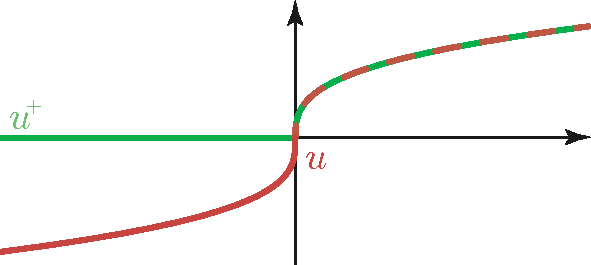
\includegraphics[trim=0cm 0cm 0cm 0cm, clip, scale=0.65]{images/partepositiva}
	\end{center}
\end{minipage}
\begin{minipage}{0.5\textwidth}
	\begin{center}
		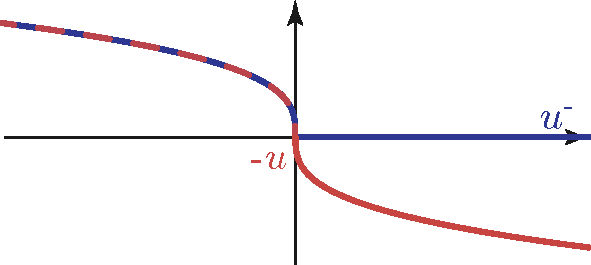
\includegraphics[trim=0cm 0cm 0cm 0cm, clip, scale=0.65]{images/partenegativa}
	\end{center}
\end{minipage}\vspace{4mm}\\
Tornando quindi a $\funz{f}{X}{\complexset}$, possiamo ottenere $f$ come combinazione lineare di quattro funzioni reali \textit{non negative}.
\begin{equation}
	f=\left(\Re f\right)+i\left(\Im f\right)=\left(\left(\Re f\right)^{+}-\left(\Re f\right)^{-}\right)+i\left(\left(\Im\right)^{+}-\left(\Im\right)^{-}\right)
\end{equation}
Con la prossima proposizione dimostreremo che le funzioni qui definite sono tutte integrabili.
\begin{proposition}[Integrabilità delle parti positive e negative delle parti reali e immaginarie]\label{integrabilitàpartiposnegrealimm}
	Se $f\in\mathcal{L}^{1}\left(\mu\right)$, allora $\left(\Re f\right)^{\pm},\ \left(\Im f\right)^{\pm}\in\mathcal{L}^{1}\left(\mu\right)$.
\end{proposition}
\begin{demonstration}
	Poiché $f\in\mathcal{L}^{1}\left(\mu\right)$, allora $\Re f$ e $\Im f$ sono misurabili; ne consegue che $\left(\Re f\right)^{\pm},\ \left(\Im f\right)^{\pm}\in\mathcal{L}^{1}\left(\mu\right)$ sono misurabili\footnote{Si vedano le ‘‘Note aggiuntive'', a pag. \pageref{misuraparterealeimm}.}, reali e non negative, dunque coincidono con il loro modulo.\\
	Poiché ogni funzione misurabile, reale, non negativa è integrabile, ciò implica che la seconda ipotesi per l'integrabilità è soddisfatta e quindi vale la tesi.
\end{demonstration}
\section{Passo 3: funzioni complesse integrabili}
Avendo enunciato tutte le premesse del caso, siamo nelle condizioni di enunciare il terzo passo dell'integrale di Lebesgue.
\begin{define}[Integrale di Lebesgue per funz. a valori complessi, integrabili]
	Sia $\funz{f}{\left(X,\mathcal{M},\mu\right)}{\complexset}$ funzione \textit{integrabile}. Posto
	\begin{equation*}
		f=\left(\Re f\right)^{+}-\left(\Re f\right)^-+i\left[\left(\Im f\right)^{+}-\left(\Im f\right)^{-}\right]
	\end{equation*}
si definisce l'\textit{integrale esteso ad E di $f$ rispetto alla misura $\mu$} come
\begin{equation}
	\int_Efd\mu\coloneqq\int_E\left(\Re f\right)^{+}d\mu-\int_E\left(\Re f\right)^{-}+i\left(\int_E\left(\Im f\right)^{+}d\mu-\int_E\left(\Im f\right)^{-}d\mu\right)
\end{equation}
\end{define}
\begin{observe}
	L'ipotesi $f\in\mathcal{L}^{1}\left(\mu\right)$ implica, come dice la proposizione \ref{integrabilitàpartiposnegrealimm}, che $\left(\Re f\right)^{\pm}$, $\left(\Im_f\right)^{\pm}\in\mathcal{L}^1\left(\mu\right)$ e quindi vale
	\begin{equation*}
		\int_X\left(\Re f\right)^{\pm}d\mu<+\infty\quad \int_X\left(\Im f\right)^{\pm}d\mu<+\infty
	\end{equation*}
	Di conseguenza, tale integrale esiste finito in $\complexset$. Se infatti le quattro funzioni ottenute decomponendo $f$ non fossero integrabili, allora potrebbero capitare delle situazioni in cui \textit{due degli integrali} della scomposizione danno la \textit{forma indeterminata} $\infty-\infty$.
\end{observe}
\begin{property}[Proprietà dell'integrale di Lebesgue per funzioni a valori in {$\complexset$}]
	Sia $\left(X,\mathcal{M},\mu\right)$ uno spazio di misura.
	\begin{enumerate}
		\item \textbf{Linearità:}
		\begin{equation}
			\int_X\left(\alpha f+\beta g\right)d\mu=\alpha\int_Xfd\mu+\beta\int_Xgd\mu,\ \forall f,g\in\mathcal{L}^1\left(\mu\right),\ \forall\alpha,\ \beta\in\complexset
		\end{equation}
		\item \textbf{Monotonia rispetto al modulo:}
		\begin{equation}
			\abs{\int_Xfd\mu}\leq \int_X\abs{f}d\mu,\ \forall f\in\mathcal{L}^1\left(\mu\right)
		\end{equation}
	\item $\sigma$-\textbf{additività rispetto al dominio:} se $\displaystyle E=\bigcup_{n\geq 1}E_n,\ \forall E_n\in\mathcal{M}\colon E_i\cap E_j=\emptyset,\ \forall i\neq j$, allora
	\begin{equation}
		f\in\mathcal{L}^1\left(\mu\right)\implies \int_Efd\mu=\sum_{n\geq 1}\int_{E_n}fd\mu
	\end{equation}
\item \textbf{Assoluta continuità:}
\begin{equation}
	f\in\mathcal{L}^{1}\left(\mu\right)\implies \forall \epsilon>0,\ \exists \delta >0\colon\forall E\in\mathcal{M}\colon \mu\left(E\right)<\delta\implies\abs{\int_E fd\mu}<\epsilon
\end{equation}
in altre parole, l'integrale si può rendere arbitrariamente più piccolo in modulo a patto di integrare su un dominio di misura sufficientemente piccola.
\end{enumerate}
\end{property}
\begin{demonstration}
	Dimostriamo l'assoluta continuità (punto 4).\\
	Consideriamo $\funz{f}{X}{\complexset}$ con $f\in\mathcal{L}^1\left(\mu\right)$; sappiamo che $f$ è misurabile e pertanto anche $\funz{\lvert f\rvert}{X}{\left[0,+\infty\right)}$ la è.\\
	Consideriamo la misura
	\begin{equation*}
		\funztot{\mu_{|f|}}{\mathcal{M}}{\left[0,+\infty\right]}{E}{\int_E\abs{f}d\mu}
	\end{equation*}
Essa è assolutamente continua rispetto a $\mu$. Inoltre, $\mu_{\abs{f}}$ è finita perché $f\in\mathcal{L}^1\left(\mu\right)$ e quindi
\begin{equation*}
	\mu_{\abs{f}}(X)=\int_X\abs{f}d\mu<+\infty
\end{equation*}
Per la caratterizzazione delle misure finite assolutamente continue rispetto a $\mu$ si ha
\begin{equation*}
	\forall \epsilon >0,\ \exists \delta > 0\colon E\in\mathcal{M},\ \mu\left(E\right)<\delta\implies \mu_{\abs{f}}\left(E\right)=\int_E\abs{f}d\mu<\epsilon
\end{equation*}
Si ha quindi
\begin{equation*}
	\forall \epsilon > 0,\ \exists \delta >0\colon \exists E\in\mathcal{M},\ \mu\left(E\right)<\delta\implies \abs{\int_Efd\mu}\underset{\substack{\text{prop. }2\\\text{dell'int.}}}{\leq}\int_E\abs{f}d\mu<\epsilon\implies \abs{\int_Efd\mu}<\epsilon\qedhere
\end{equation*}
\end{demonstration}
\subsection{Teorema della convergenza dominata}\index{teorema!della convergenza dominata}
\begin{theorema}[Teorema della convergenza dominata]\label{thmconvergenzadominata}
Siano $\left(X,\mathcal{M},\mu\right)$ uno spazio di misura e $\funz{f_n,f}{X}{\complexset}$ con $n\geq 1$ tali che
\begin{enumerate}[label=(\alph*)]
	\item 	$f_n$ sono misurabili.
	\item 	$\displaystyle \lim_{n\to+\infty}f_n(x)=f(x),\ \forall x\in X$
	\item 	Esiste una funzione $g\in \mathcal{L}^{1}\left(\mu\right)$ tale per cui
\begin{equation*}
	\abs{f_n(x)}\leq g(x),\ \forall n\geq 1,\ \forall x\in X
\end{equation*}
\end{enumerate}
Allora
\begin{enumerate}
	\item $f\in L^{1}\left(\mu\right)$.
	\item $\displaystyle\lim_{n\to+\infty}\int_X\abs{f_n-f}d\mu=0$
	\item Vale il \textbf{passaggio al limite sotto segno di integrale}\index{passaggio al limite sotto segno di integrale}:
	\begin{equation}
		\lim_{n\to+\infty}\int_Xf_nd\mu=\int_Xfd\mu
	\end{equation}
\end{enumerate}
\end{theorema}
\begin{demonstration}
	Poiché $f_n$ è una successione di funzioni misurabili che converge puntualmente a $f$, $\forall x\in X$, $f$ è una funzione misurabile. Inoltre, dato che tutti gli elementi della successione $f_n$ sono maggiorati (in modulo) da $g$, si ha per monotonia del limite che
	\begin{equation*}
		\circled[red]{\vardiamond}\quad \abs{f}\leq g
	\end{equation*}
	Allora, applicando i moduli ai membri della disequazione vale $\abs{f}\leq\abs{g}$. Integrando rispetto a Lebesgue, per monotonia rispetto all'integranda si ha
	\begin{equation*}
		\int_X\abs{f}d\mu\leq \int_X \abs{g}d\mu<+\infty
	\end{equation*}
	in quanto $g\in \mathcal{L}^1\left(\mu\right)$; segue che $f\in \mathcal{L}^1\left(\mu\right)$.\\
	Osserviamo che
	\begin{align*}
		\abs{f_n-f}&\leq \abs{f_n}+\abs{f}&\text{(disuguaglianza triangolare)}\\
		&\leq2g&\text{(per $\circled[red]{\vardiamond}$)}
	\end{align*}
	da cui segue che $2g-\abs{f_n-f}\geq 0$ e quindi sono funzioni non negative. Poiché le $2g-\abs{f_n-f}$ sono misurabili in quanto somma di funzioni in $\mathcal{L}^1\left(\mu\right)$ (e quindi misurabili), possiamo applicare il \textit{lemma di Fatou} a tali funzioni e ottenere
	\begin{gather*}
		\int_X\left(\liminf_{n\to+\infty}2g-\abs{f_n-f}\right)d\mu\leq\liminf_{n\to+\infty}\int_X\left(2g-\abs{f_n-f}\right)d\mu\\
		\viff\\
		\int_X 2gd\mu-\int_X\liminf_{n\to+\infty}\abs{f_n-f}d\mu\leq\int_X 2gd\mu+\liminf_{n\to+\infty}\left(-\int_X\abs{f_n-f}d\mu\right)
	\end{gather*}
	ma
	\begin{equation*}
		\int_X\liminf_{n\to+\infty}\abs{f_n-f}d\mu=0
	\end{equation*}
	in quanto per ipotesi $\displaystyle\lim_{n\to+\infty}f_n=f\iff\lim_{n\to+\infty}\abs{f_n-f}=0$; segue che $\liminf$ e $\lim$ coincidono con valore $0$ e pertanto anche l'integrale risulta nullo.\\
	Inoltre, notiamo che
	\begin{equation*}
		\int_X\abs{f_n-f}d\mu
	\end{equation*}
	è una successione a valori non negativi, dunque per le proprietà del massimo e minimo limite\footnote{Nell'approfondimento ‘‘Massimo e minimo limite'', a pag. \pageref{maxminlegame} è possibile trovare la dimostrazione di questo risultato insieme ad altri relativi al limsup e liminf.} si ha
	\begin{equation*}
		\liminf_{n\to+\infty}\left(-\int_X\abs{f_n-f}d\mu\right)=-\limsup_{n\to+\infty}\left(\int_X\abs{f_n-f}d\mu\right)
	\end{equation*}
	Allora otteniamo
	\begin{equation*}
		\int_X 2gd\mu\leq\int_X 2gd\mu-\limsup_{n\to+\infty}\left(\int_X\abs{f_n-f}d\mu\right)
	\end{equation*}
	Dato che $g\in \mathcal{L}^1\left(\mu\right)$ è non negativa, si ha  
	\begin{equation*}
		\int_X2gd\mu=2\int_X\abs{g}d\mu<+\infty
	\end{equation*}
	Possiamo dunque sottrarre
	\begin{equation*}
		\int_X 2gd\mu
	\end{equation*}
	da entrambi i membri della disequazione e ottenere
	\begin{equation*}
		\circled[blue]{\spadesuit}\quad \limsup_{n\to+\infty}\int_X\abs{f_n-f}d\mu\leq 0
	\end{equation*} 
	Notiamo che se una successione di numeri reali non negativi non converge a $0$, allora il massimo limite è positivo.\footnote{Infatti, se $a_n\geq 0,\ \forall n\in\naturalset$, allora anche il limite $\displaystyle \lim_{n\to+\infty}a_n$ sarà non negativo.  Tuttavia, poiché tale successione ammette limite, allora esso coincide con il suo massimo limite. Segue immediatamente che
	\begin{equation*}
		\lim_{n\to+\infty}a_n\neq0\implies \lim_{n\to+\infty}a_n>0\implies \limsup_{n\to+\infty}a_n>0
	\end{equation*}} Per contronominale, se il massimo limite di numeri reali non negativi \textit{non} è positivo, allora la serie converge a $0$ necessariamente. Poiché vale \circled[blue]{\spadesuit}, allora ciò implica la prima tesi:
	\begin{equation*}
		\lim_{n\to+\infty}\int_X\abs{f_n-f}d\mu=0
	\end{equation*}
	Infine, poiché l'integrale di Lebesgue è monotono rispetto al modulo, si ha
	\begin{equation*}
		0=\lim_{n\to+\infty}\int_X\abs{f_n-f}d\mu\geq\lim_{n\to+\infty}\abs{\int_X\left(f_n-f\right)d\mu}\ge 0
	\end{equation*}
	e quindi
	\begin{equation*}
		\lim_{n\to+\infty}\abs{\int_X \left(f_n-f\right)d\mu}=0\implies\lim_{n\to+\infty}\int_X\left(f_n-f\right)d\mu=0\implies\lim_{n\to+\infty}\int_X f_nd\mu=\int_X fd\mu
	\end{equation*}
	ottenendo la seconda e ultima tesi.
\end{demonstration}
\section{Tra integrale di Riemann e integrale di Lebesgue}
Nell'excursus storico abbiamo visto come l'\textit{integrale di Lebesgue} e le sue successive astrazioni di inizio '900 siano state la risposta a due domande che indirizzarono gli studi di Analisi del XIX secolo:
\begin{itemize}
	\item Come si può allargare la classe delle funzioni integrabili?
	\item Come si può caratterizzare l'insieme dei punti di discontinuità di una funzione integrabile secondo Riemann?
\end{itemize}
Con i tre passi precedentemente esposti abbiamo costruito l'integrale astratto di Lebesgue e risposto alla prima domanda, mentre rimane al momento aperta la seconda; in particolare, nel caso di funzioni da $\realset$ a $\realset$, sorge la questione: \textit{che relazione c'è tra l'integrale di Riemann e l'integrale di Lebesgue?}\\
Nel caso di funzioni limitate su un intervallo chiuso e che sono Riemann-integrabili scopriamo che tali integrali coincidono.
\begin{theoremaqed}[Integrale proprio di Riemann implica integrale di Lebesgue]
	Sia $\funz{f}{\left[a,b\right]}{\realset}$ limitata e misurabile. Allora
	\begin{equation}
		f\in\mathcal{R}\left(\left[a,b\right]\right)\implies f\in\mathcal{L}^1\left(\left[a,b\right],m_1\right)
	\end{equation}
e
\begin{equation}
	\int_{\left[a,b\right]}\abs{f}dm_1=\int_{a}^{b}f(x)dx\qedhere
\end{equation}
\end{theoremaqed}
% TO DO: add cenni dimostrazione
\begin{observes}~
	\begin{itemize}
		\item Il viceversa non è vero: come abbiamo già visto\footnote{Si veda pag. \pageref{funzionedirichletintegrale}.}, la funzione di Dirichlet è integrabile secondo Lebesgue ma non secondo Riemann.
		\item L'ipotesi di misurabilità è in realtà ridondante: come si potrà vedere con i risultati della sezione successiva, ogni funzione limitata e Riemann-integrabile è sempre misurabile rispetto alla misura di Lebesgue $m_1$.
	\end{itemize}
\end{observes}
Situazione differente si ha con l'integrale improprio di Riemann: infatti, può capitare che ci siano funzioni integrabili (almeno impropriamente) secondo Riemann ma \textit{non} secondo Lebesgue!
\begin{theoremaqed}[Integrale improprio di Riemann e integrale di Lebesgue]\label{integraleimproprioriemannlebesgue}
	Sia $\funz{f}{\left[a,+\infty\right]}{\realset}$ misurabile tale che $f\in\mathcal{R}\left(\left[a,b\right]\right)$ per ogni $b>a$. Allora
	\begin{enumerate}
		\item Vale la relazione
		\begin{equation}
			\int_{\left[a,+\infty\right)}\abs{f}dm_1=\int_{0}^{+\infty}\abs{f(x)}dx\in\left[0,+\infty\right]
		\end{equation}
		\item Se l'integrale improprio di Riemann di $f$ su $\left[a,+\infty\right)$ converge \textit{assolutamente} allora $f$ è integrabile secondo Lebesgue su $\left[a,+\infty\right)$ e
		\begin{equation}
			\int_{\left[a,+\infty\right)}fdm_1=\int_{a}^{+\infty}f(x)dx\in\realset\qedhere
		\end{equation}
	\end{enumerate}
\end{theoremaqed}
\begin{observe}
	CI sono risultati analoghi per gli integrali impropri di Riemann della forma
	\begin{align*}
		\int_{-\infty}^{b}f(x)dx&=\lim_{a\to-\infty}\int_{a}^{b}f(x)dx\\
		\int_{a}^{\gamma}f(x)dx&=\lim_{b\to \gamma^{-}}\int_{a}^{b}f(x)dx\\
		\int_{\gamma}^{b}f(x)dx&=\lim_{a\to \gamma^{+}}\int_{a}^{b}f(x)dx
	\end{align*}
\end{observe}
\begin{attention}
	Se l'integrale improprio di Riemann di $f$ su $\left[a,+\infty\right)$ converge ma non \textit{assolutamente} allora $f$ \textit{non} è integrabile secondo Lebesgue su $\left[a,+\infty\right)$.
\end{attention}
\begin{example}
	Consideriamo la funzione
	\begin{equation*}
		f(x)=\frac{\sin x}{x}
	\end{equation*}
	sull'intervallo $\left[\pi,+\infty\right)$. Mostriamo che:
	\begin{enumerate}
		\item L'integrale di $f$ secondo Riemann converge semplicemente.
		\item L'integrale di $f$ secondo Riemann \textit{non} converge assolutamente.
		\item La funzione $f$ \textit{non} è integrabile secondo Lebesgue.
	\end{enumerate}
\begin{enumerate}[label=\Roman*]
	\item Integrando per parti si ha
	\begin{align*}
		\int_{\pi}^{+\infty}\frac{\sin x}{x}dx&=\lim_{R\to+\infty}\int_{\pi}^{R}\frac{\sin x}{x}dx=\lim_{R\to+\infty}\left[-\frac{\cos x}{x}\Big|^{R}_{\pi}-\int_{\pi}^{R}\frac{\cos x}{x^2}dx\right]\\
		&=\lim_{R\to+\infty}\biggl[\underbrace{-\frac{\cos R}{R}}_{\substack{\to 0\text{ per}\\R\to+\infty}}+\cos \pi-\int_{\pi}^{R}\frac{\cos x}{x^2}dx\biggr]=-1-\int_{\pi}^{+\infty}\frac{\cos x}{x^2}dx
	\end{align*}
dato che
\begin{equation*}
	0\leq \abs{\frac{\cos x}{x^2}}\leq \frac{1}{x^2}
\end{equation*}
e
\begin{equation*}
	\int_{\pi}^{\infty}\frac{1}{x^2}
\end{equation*}
converge, allora
\begin{equation*}
	\int_{\pi}^{+\infty}\abs{\frac{\cos x}{x^2}}
\end{equation*}
converge e dunque
\begin{equation*}
	\int_{\pi}^{+\infty}\frac{\sin x}{x}dx
\end{equation*}
converge (assolutamente). Ne consegue che l'integrale di $f(x)$ è \textit{semplicemente convergente}.
\item Osserviamo che, per ogni $n\in\naturalset$, si ha
\begin{align*}
	\int_{\pi}^{n\pi}\frac{\abs{\sin x}}{x}dx&=\sum_{k=1}^{n-1}\int_{k\pi}^{\left(k+1\right)\pi}\frac{\abs{\sin x}}{x}dx&\\
	&>\sum_{k=1}^{n-1}\frac{1}{\left(k+1\right)\pi}\int_{k\pi}^{\left(k+1\right)\pi}\abs{\sin x}dx&\text{($\nicefrac{1}{x}$ decrescente)}\\
	&=\sum_{k=1}^{n-1}\frac{2}{\left(k+1\right)\pi}=\frac{2}{\pi}\sum_{k=2}^{n}\frac{1}{k}&
\end{align*}
operando nell'ultimo passaggio un cambio di indice $k-1\to k$. Passando al limite per $n\to+\infty$ si ha
\begin{equation*}
	\int_{\pi}^{+\infty}\frac{\abs{\sin x}}{x}dx>\frac{2}{\pi}\sum_{k=2}^{+\infty}\frac{1}{k}=\frac{2}{\pi}\left[\sum_{k=1}^{+\infty}\frac{1}{k}-1\right]
\end{equation*}
Poiché l'integrale è minorato dalla \textit{serie armonica}, che sappiamo essere \textit{divergente}, allora l'integrale diverge e quindi l'integrale della funzione $f(x)$ \textit{non} converge \textit{assolutamente}.
\item Per il primo punto del teorema \ref{integraleimproprioriemannlebesgue} vale
\begin{equation*}
	\int_{\left[\pi,+\infty\right)}\abs{\frac{\sin x}{x}}dm_1=\int_{\pi}^{\infty}\abs{\frac{\sin x}{x}}dx=+\infty
\end{equation*}
Poiché l'integrale improprio di Riemann \textit{non} converge assolutamente, segue che $f$ non è integrabile su $\left[\pi,+\infty\right)$ e pertanto non ammette integrale secondo Lebesgue.
\end{enumerate}
\end{example}
Sulla base di questi risultati siamo finalmente in grado di rispondere al secondo quesito: con una certa ironia, la caratterizzazione dell'insieme dei punti di discontinuità di una funzione integrabile secondo Riemann è basata sulla \textbf{misura di Lebesgue}.
\begin{theoremaqed}[Caratterizzazione delle funzioni integrabili secondo Riemann]
	Sia $\funz{f}{\left[a,b\right]}{\realset}$ limitata e sia $D_f$ l'insieme delle discontinuità di $f$. Se $m_1$ è la misura  di Lebesgue unidimensionale, allora
	\begin{equation}
		f\in\mathcal{R}\left(\left[a,b\right]\right)\iff m_1\left(D_f\right)=0\qedhere
	\end{equation}
ossia $f$ limitata è Riemann-integrabile su $\left[a,b\right]$ se e solo se $f$ è continua \textbf{q.o.} su $\left[a,b\right]$.
\end{theoremaqed}
\begin{example}
	Sia $C\subseteq\left[0,1\right]$ l'insieme di Cantor e sia $f=\chi_C$ la funzione caratteristica su tale insieme.
	Si ha che $D_f=\partial C$, ma poiché $C$ è un chiuso con interno vuoto, allora
	\begin{equation*}
		D_f=\partial C=C
	\end{equation*}
	Essendo $m_1\left(C\right)=0$, $f$ è integrabile secondo Riemann su $\left[0,1\right]$.
\end{example}
\section{Il ruolo degli insiemi di misura nulla}
Abbiamo appena visto come una funzione è integrabile secondo Riemann se e solo se l'insieme delle sue discontinuità è un insieme di misura nulla. In altre parole, una funzione è integrabile secondo Riemann su un dato intervallo se e solo se essa è continua, tolto al più un insieme misurabilmente nullo di discontinuità.\\
Più in generale, ha senso parlare di proprietà valide su un particolare dominio tolto un insieme di misura nulla: poiché queste proprietà non valgono su insiemi la cui \textit{rilevanza è minima}, quantomeno dal punto della \textit{misura}, possiamo definire tale proprietà come \textit{quasi ovunque valida}.
\begin{define}[Proprietà quasi ovunque valida]
	Sia $\left(X,\mathcal{M},\mu\right)$ uno spazio di misura. Si dice che una proprietà $P$ vale \textbf{‘‘quasi ovunque''} (\textbf{q.o.})\index{proprietà quasi ovunque valida} o ‘‘$\mu$\textbf{-quasi ovunque}'' se vale in tutto $X$ tranne eventualmente su un insieme di misrua $\mu$ nulla. In altre parole, deve esistere un insieme $N\in\mathcal{M}$ con $\mu(N)=0$ tale che $\forall x\in X\setminus N$ vale tale proprietà $P$.
\end{define}
\begin{observe}
	Dalla definizione di per sè \textit{non} è richiesto che l'insieme
	\begin{equation*}
		E=\{x\in\ X\mid P(x)\text{non vale}\}
	\end{equation*}
	sia misurabile, ma solamente che \textit{sia contenuto} in un insieme misurabile e di misura nulla: questo significa che a priori $E$ non è misurabile!\\
	Tuttavia, se la misura è \textit{completa}, allora anche $E$ risulta essere misurabile e di misura nulla.
\end{observe}
\begin{examplewt}[Uguaglianza quasi ovunque]
	Siano $\funz{f,g}{X}{\complexset}$ misurabili. Allora
	\begin{equation}
		f=g\ \text{\textbf{q.o.}}\iff \text{Posto}\ E=\{x\in\ X\mid f(x)\neq g(x)\},\ \mu\left(E\right)ù=0
	\end{equation}
	Poiché $E=(f-g)^{-1}\left(\complexset\setminus\{0\}\right)$, $f,\ g$ sono misurabili e $\complexset\setminus\{0\}$ è aperto, allora $E$ è misurabile e la definizione è ben posta.\\
	Inoltre, si può notare che si può estendere la stessa definizione di uguaglianza \textbf{q.o.} a funzioni $f,\ g$ \textit{non} necessariamente misurabili con codominio uno spazio topologico, a patto di supporre che la misura $\mu$ sia \textit{completa}.
\end{examplewt}
\begin{example}
	Consideriamo la funzione di Dirichlet $f=\chi_{\left[0,1\right]\cap\rationalset}$:
	\begin{equation*}
		f(x)=\begin{cases}
			\begin{array}{ll}
				1&\text{se }x\in\left[0,1\right]\cap\rationalset\\
				0&\text{se }x\in\left[0,1\right]\setminus\rationalset
			\end{array}
		\end{cases}
	\end{equation*}
Sappiamo che $m_1\left(\left[0,1\right]\cap\rationalset\right)=0$, quindi
\begin{equation*}
	\left\{x\in\left[0,1\right]\mid f(x)\neq 0\right\}=\left[0,1\right]\cap \rationalset
\end{equation*}
ha misura nulla e pertanto la funzione di Dirichlet è \textit{quasi ovunque} la funzione identicamente \textit{nulla}.
\end{example}
\begin{property}[Ruolo degli insiemi di misura nulla nell'integrazione]
Sia $\left(X,\mathcal{M},\mu\right)$ uno spazio di misura. Allora
\begin{enumerate}
	\item Se $\funz{f}{X}{\complexset}$ e $f\in\mathcal{L}^{1}\left(\mu\right)$, allora
	\begin{equation}
		\forall E\in\mathcal{M},\ \mu\left(E\right)=0\implies \int_Efd\mu=0
	\end{equation}
\item Se $\funz{f,g}{X}{\complexset}$ e $f,g\in\mathcal{L}^{1}\left(\mu\right)$, allora
\begin{equation}
	f=g\ \text{\textbf{q.o.}}\implies \int_Xfd\mu=\int_Xgd\mu
\end{equation}
\item Se $\funz{f}{X}{\left[0,+\infty\right)}$ misurabile, allora
\begin{equation}
	\int_X fd\mu=0\implies f=0 \text{\textbf{q.o.} in }X
\end{equation}
\end{enumerate}
\end{property}
\begin{demonstration}~{}
	\begin{enumerate}[label=\Roman*]
		\setcounter{enumi}{1}
		\item Posto
		\begin{equation*}
			E=\left\{x\in X\mid f(x)\neq g(x)\right\}
		\end{equation*}
	si ha $\mu\left(E\right)=0$. Allora
	\begin{equation*}
		\int_Xfd\mu=\int_{X\setminus E}fd\mu+\int_Efd\mu=\int_{X\setminus E}gd\mu+0=\int_{X\setminus E}gd\mu+\int_Egd\mu=\int_Xgd\mu
	\end{equation*}
	\item Sia
		\begin{equation*}
			E=\left\{x\in X\mid f(x)\neq 0\right\}=\bigcup_{n\geq 1}\left\{x\in X\mid f(x)>\frac{1}{n}\right\}=\bigcup_{n\geq 1}E_n
		\end{equation*}
	Osserviamo che $E_n=f^{-1}\left(\left(\frac{1}{n},+\infty\right)\right)\in\mathcal{M}$ in quanto è controimmagine di un aperto tramite una funzione misurabile; su ha allora
	\begin{align*}
		0&=\int_Xfd\mu&\\
		 &\leq\int_{E_n}fd\mu&\text{(monotonia dell'integrale rispetto al dominio)}\\
		 &\leq\int_{E_n}\frac{1}{n}d\mu&\text{(monotonia rispetto l'integranda)}\\
		 &=\frac{1}{n}\mu\left(E_n\right)\leq 0&
	\end{align*}
	Segue dunque che $\mu\left(E_n\right)=0,\ \forall n\geq 1$; utilizzando la $\sigma$-subadditività della misura vediamo che
	\begin{equation*}
		\mu\left(E\right)=\mu\left(\bigcup_{n\geq 1}E_n\right)\leq\sum_{n=1}^{+\infty}\mu\left(E_n\right)=0\implies \mu\left(E\right)=0
	\end{equation*}
	Vale dunque la tesi.\qedhere
	\end{enumerate}
\end{demonstration}
Avendo definito il concetto di proprietà quasi ovunque valida, possiamo enunciare un'altra versione dello \textit{scambio tra integrale e serie}, questo risultato che segue dal \textit{teorema della convergenza dominata}.
\begin{theorema}[Scambio tra integrale e serie per funzioni integrabili]
	Sia $\left(X,\mathcal{M},\mu\right)$ uno spazio di misura. Siano $\funz{f_n}{X}{\complexset}$ integrabili. Supponiamo che
	\begin{equation*}
		\sum_{n=1}^{+\infty}\int_X\abs{f_n}d\mu<+\infty
	\end{equation*}
Allora
\begin{enumerate}
	\item $\displaystyle f(x)=\sum_{n=1}^{+\infty}f_n(x)$ è definita \textbf{q.o.} in $X$.
	\item $f\in\mathcal{L}^{1}\left(\mu\right)$
	\item Vale lo \textit{scambio tra integrale e serie}\index{scambio tra integrale e serie}:
	\begin{equation}
		\int_Xfd\mu=\int_X\left(\sum_{n=1}^{+\infty}f_n\right)d\mu=\sum_{n=1}^{+\infty}\int_Xfd\mu\in\complexset
	\end{equation}
\end{enumerate}
\end{theorema}
%\part{Omotopia}
%\labelPart{second}
%% SVN info for this file
\svnidlong
{$HeadURL$}
{$LastChangedDate$}
{$LastChangedRevision$}
{$LastChangedBy$}

\chapter{Convergenza di funzioni, parte seconda}
\labelChapter{convergenzafunzioniseconda}

\begin{introduction}
	‘‘È una rottura pensare alle convergenze, ma a volte bisogna davvero farlo.''
	\begin{flushright}
		\textsc{Sinai Robins,} ricordandosi delle innumerevoli convergenze di funzioni tre giorni prima dell'esame di Analisi Matematica 3.
	\end{flushright}
\end{introduction}
\lettrine[findent=1pt, nindent=0pt]{D}{allo} \textbf{[COMPLETARE.]} % TO DO: completare
\section{Dallo spazio delle funzioni integrabili allo 1-spazio di Lebesgue}
Ricordiamo che, dato uno spazio di misura $\left(X,\mathcal{M},\mu\right)$ si definisce lo spazio delle funzioni integrabili
\begin{equation}
	\mathcal{L}^{1}=\left\{\funz{f}{X}{\complexset}\text{ misurabili}\middle| \int_X\abs{f}d\mu<+\infty\right\}
\end{equation}
il quale è un spazio vettoriale con le operazioni di somma di funzioni e prodotto di una funzione per uno scalare complesso.\\
Vogliamo ora introdurre una struttura \textit{metrica} in $\mathcal{L}^1\left(\mu\right)$; nello specifico, cerchiamo una \textit{norma} - in questo modo potremo avvalerci di risultati che sono validi solo in \textit{spazi normati}. Possiamo considerare come potenziale candidata la funzione
\begin{equation}
	\funztot{N}{\mathcal{L}^1\left(\mu\right)}{\left[0,+\infty\right)}{f}{\int_X\abs{f}d\mu}
\end{equation}
Tuttavia, la suddetta è una \textbf{pseudonorma} in quanto soddisfa due delle tre proprietà della norma, ma non la \textit{prima}: può valere zero per altre funzione oltre quella nulla. Infatti:
\begin{enumerate}
	\item[1.] $\displaystyle f=0\implies \int_X\abs{f}d\mu=0$ ma $\displaystyle \int_X\abs{f}d\mu=0\implies f$ \textbf{q.o.} in $X$.
\end{enumerate}
Come precedentemente detto, le proprietà 2 e 3 sono verificate:
\begin{enumerate}
	\item[2.] $N\left(\lambda f\right)=\abs{\lambda}N\left(f\right),\ \forall f\in\mathcal{L}^1\left(\mu\right),\ \forall \lambda \in \complexset$.
	\item[3.] $N\left(f+g\right)\leq N\left(f\right)+N\left(g\right),\ \forall f,g\in\mathcal{L}^{1}\left(\mu\right)$.
\end{enumerate}
Per risolvere il problema, si introduce la relazione
\begin{equation}
	f,g\in\mathcal{L}^{1}\left(\mu\right)\colon f\sim g\iff f=g\text{ \textbf{q.o.} in }X
\end{equation}
che si dimostra essere di equivalenza in $\mathcal{L}^{1}\left(\mu\right)$.\\
Si definisce allora lo $1$\textbf{-spazio di Lebesgue}\index{spazio!di Lebesgue}
\begin{equation}
	L^{1}\left(\mu\right)=\frac{\mathcal{L}^{1}\left(\mu\right)}{\sim}
\end{equation}\\
\begin{notate}
	Invece che indicare gli elementi di $L^{1}\left(\mu\right)$ come classi di equivalenza $\left[f\right]$ (dove $f\in\mathcal{L}^{1}\left(\mu\right)$), faremo un \textit{abuso di notazione} e indicheremo solo $f\in L^{1}$.
\end{notate}
In $L^1{\left(\mu\right)}$ possiamo finalmente definire una vera e onesta norma:
\begin{equation}
	\funztot{\lvert\cdot\rvert}{L^{1}\left(\mu\right)}{\left[0,+\infty\right)}{\left[f\right]}{\lvert\left[f\right]\rvert_1=\int_X\abs{f}d\mu}
\end{equation}
Questa norma è ben posta come funzione in $L^1\left(\mu\right)$ in quanto \textit{non} dipende dal \textit{rappresentante} scelto:
\begin{equation*}
	g\in\left[f\right]\iff f=g\text{ \textbf{q.o.} in }X\implies \int_X\abs{g}d\mu=\int_X\abs{f}d\mu
\end{equation*}
\begin{example}
	Consideriamo lo spazio di misura $\left(\naturalset,\setpart{\naturalset},\mu_c\right)$ con $\mu_c$ la misura conteggio:
	\begin{equation*}
		\mu_c\left(E\right)=\begin{cases}
			\begin{array}{ll}
				\# E &\text{se }E\text{ è finito}\\
				+\infty &\text{altrimenti}
			\end{array}
		\end{cases}\quad\forall E\in\setpart{\naturalset}
	\end{equation*}
	Ricordiamo che, data la successione $\funz{f}{\naturalset}{\left[0,+\infty\right]}$ (dove $f\left(n\right)\coloneqq f_n$), allora come conseguenza del teorema di convergenza monotona si ha
	\begin{equation*}
		\int_\naturalset fd\mu_c=\sum_{n=1}^{+\infty}f_n
	\end{equation*}
	In questo caso si ha
	\begin{equation*}
		\mathcal{L}^1\left(\mu_c\right)=\left\{\funz{f}{\naturalset}{\complexset}\mid\sum_{n=1}^{+\infty}\abs{f_n}=\int_X\abs{f}d\mu_c<+\infty\right\}
	\end{equation*}
	e quindi la norma in $L^1$ è la serie dei moduli
	\begin{equation*}
		\norm{f}_1=\sum_{n=1}^{+\infty}\abs{f_n}
	\end{equation*}
\end{example}
Come sappiamo, se uno spazio normato è completo valgono diversi risultati teorici e pratici di estrema importanza, come ad esempio il criterio di Cauchy. Si dimostrerà a \textsc{Istituzioni di Analisi Matematica} che anche $L^1$ è uno spazio normato completo.
\begin{theoremaqed}[{$L^1$} è completo]
	Lo spazio normato $\left(L^1\left(\mu\right),\norm{\cdot}_1\right)$ è completo.
\end{theoremaqed}
\begin{observe}
	Se si considero lo spazio delle funzioni continue $\mathcal{C}\left(\left[a,b\right];\realset\right)$, allora in esso la funzione
	\begin{equation*}
		\funztot{\ }{\mathcal{C}\left(\left[a,b\right];\realset\right)}{\left[0,+\infty\right]}{f}{\lvert f\rvert_1\int_{a}^{b}\abs{f(x)}dx}
	\end{equation*}
	è già una norma. Infatti
	\begin{equation*}
		\lvert f\rvert_1 = 0 \iff f\equiv 0\text{ \textbf{q.o.} in }\left[a,b\right]\iff f\equiv 0\text{ su }\left[a,b\right]\text{ perché continua}
	\end{equation*}
	Pertanto, $\mathcal{C}\left(\left[a,b\right];\realset\right)$ è normato. Lo svantaggio, tuttavia, è che esso \textit{non} è completo.Per questo motivo, nonostante ciò che comporta quozientare, conviene usare lo spazio $\left(L^1\left(\mu\right),\norm{\cdot}_1\right)$.
\end{observe}
\subsection{Eserciziamoci! Dallo spazio delle funzioni integrabili allo 1-spazio di Lebesgue}
\begin{exercise}
	Dimostrare che la relazione
	\begin{equation}
		f,g\in\mathcal{L}^{1}\left(\mu\right)\colon f\sim g\iff f=g\text{ \textbf{q.o.} in }X
	\end{equation}
	è di equivalenza in $\mathcal{L}^{1}\left(\mu\right)$
\end{exercise}
\begin{solution}
	La riflessività e la simmetria sono banalmente verificate per definizione di uguaglianza \textbf{q.o.}.\\
	Per dimostrare la transitività, si considerino le funzioni $f,g,h\in\mathcal{L}^{1}$ tali che $f=g$ \textbf{q.o.} e $g=h$ \textbf{q.o.}. Ciò significa che
	\begin{equation*}
		\mu(N_1)\coloneqq\mu\left(\{x\in X\mid f(x)\neq g(x)\}\right)=0=\mu\left(\{x\in X\mid g(x)\neq h(x)\}\right)\Coloneqq\mu(N_2)
	\end{equation*}
	Posto $N=N_1\cup N_2$, allora anche $N$ è misurabile con misura nulla.\\
	Per le leggi di De Morgan si ha che $N^C=N_1^C\cap N_2^C$, cioè per ogni $x\in N^C$ si ha $f(x)=g(x)=h(x)$. Allora
	\begin{equation*}
		N^C\subseteq\{x\in X\mid f(x)=h(x)\}\implies \{x\in X\mid f(x)\neq h(x)\}\subseteq N
	\end{equation*}
	Poiché $\{x\in X\mid f(x)\neq h(x)\}$ è misurabile e contenuto in $N$ cha ha misura nulla, allora si ha la tesi cercata.
\end{solution}
\section{Modi di convergenza}\label{modiconvergenza}
Abbiamo già visto nel \refChapterOnly{convergenzafunzioni} la convergenza uniforme e la convergenza puntuale. Noti i concetti di misura e integrale di Lebesgue, approfondiamo il tema dei modi di convergenza e le relazioni tra questi.
\paragraph{Convergenza uniforme}
\begin{define}[Convergenza uniforme]
	Consideriamo lo spazio di misura $\left(X,\mathcal{M},\mu\right)$ e le funzioni $\funz{f_n,f}{X}{\complexset}$ misurabili per ogni $n$.
	Si dice che $f_n$ \textbf{converge uniformemente}\index{convergenza!uniforme} a $f$\textbf{su} $X$ ($f_n\overset{\text{unif.}}{\to} f$) se
	\begin{equation}
		\forall \epsilon >0,\ \exists N=N\left(\epsilon\right)\colon \forall n\geq N,\ \abs{f_n(x)-f(x)}<\epsilon,\ \forall x\in X
	\end{equation}
\end{define}
Come già visto a pag. \pageref{visualizzazioneconvergenzauniforme}, se consideriamo $X\subseteq \realset$ si può visualizzare la convergenza uniforme della successione $f_n$ a $f$: arbitrariamente scelto un raggio $\epsilon$ e per $n$ sufficientemente grandi, il grafico di $f_n$ è contenuto nell'\textit{intorno tubulare} di raggio $\epsilon$ centrato sul grafico di $f$.
\begin{center}
	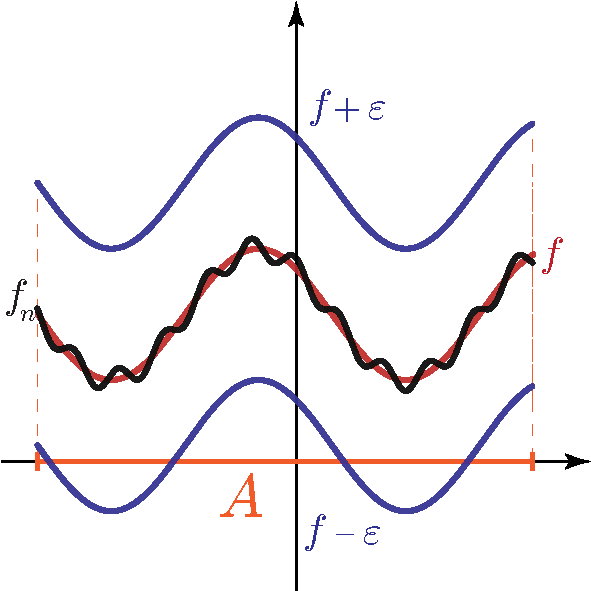
\includegraphics[trim=0cm 0cm 0cm 0cm, clip, scale=0.65]{images/visualizzazioneconvergenzauniforme.pdf}
\end{center}
\paragraph{Convergenza puntuale}
\begin{define}[Convergenza puntuale]
	Consideriamo l'insieme $X$ e le funzioni $\funz{f_n,f}{X}{\complexset}$.
	Si dice che $f_n$ \textbf{converge puntualmente}\index{convergenza!puntuale} a $f$\textbf{in} $X$ ($f_n\overset{\text{punt.}}{\to} f$) se
	\begin{equation}
		\forall x\in X,\lim_{n\to+\infty}f_n(x)=f(x)
	\end{equation}
	o, alternativamente,
	\begin{equation}
		\forall x\in X,\ \forall \epsilon >0,\ \exists N=N\left(x,\epsilon\right)\colon \forall n\geq N,\ \abs{f_n(x)-f(x)}<\epsilon
	\end{equation}
\end{define}
\begin{attention}
	Il limite della convergenza è in campo \textit{complesso}!
\end{attention}
\paragraph{Convergenza uniforme e puntuale}
Come visto in precedenza\footnote{Si veda \refChapterOnly{convergenzafunzioni}, sezione \ref{convuniformeimplicapuntuale}, pag. \pageref{convuniformeimplicapuntuale}.}, nella \textit{convergenza uniforme} il differente ordine dei quantificatori relativi alla $x$ fa sì che la soglia $N$ trovata è indipendente dal punto $x$ e quindi vale per ogni punto dell'insieme di definizione $X$, implicando pertanto la \textit{convergenza puntuale}.
\begin{multline}
	f_n\text{ converge uniformemente a }f\text{ su }X\implies\\
	\implies f_n\text{ converge puntualmente a }f\text{ in ogni punto di }X
\end{multline}
Il viceversa non è vero: abbiamo visto\footnote{Si veda nota precedente.} nella stessa sezione il caso della successione geometrica, la quale converge uniformemente solo a $f\equiv 0$ in ogni intervallo $\left[-a,a\right]\subsetneqq\left(-1,1\right),\ \forall a\in\left(0,1\right)$, mentre puntualmente in tutti i $\left(-1,1\right]$; qui di seguito riportiamo un controesempio alternativo.
\begin{example}
	Consideriamo la successione
	\begin{equation*}
		f_n(x)=\chi_{(n,n+1)}(x)=
		\begin{cases}
			\begin{array}{ll}
				1&n<x<n+1\\
				0&x\leq n\vee x\geq n+1
			\end{array}
		\end{cases}
	\end{equation*}
	Essa converge puntualmente a $f\equiv 0$:
	\begin{itemize}
		\item $\forall x\leq 0$ si ha che $f_n(x)\equiv 0,\ \forall n\in\naturalset$ e dunque banalmente $\displaystyle\lim_{n\to+\infty}f_n(x)=0$.
		\item $\forall x>0$, preso $N_x\coloneqq\floor{x}+1$ si ha che $\forall n>N_x\ f_n(x)=0$ e quindi $\displaystyle\lim_{n\to+\infty}f_n(x)=0$.
	\end{itemize}
	Tuttavia, essa non converge uniformemente a $0$ su $\realset$, dato che
	\begin{equation*}
		\lim_{n\to+\infty}\left(\sup_{x\in\realset}\abs{f_n(x)-f(x)}\right)=\lim_{n\to+\infty}\left(\sup_{x\in\realset}\abs{1-0}\right)=1\neq 0
	\end{equation*}
\end{example}
\paragraph{Convergena quasi ovunque}
\begin{define}[Convergenza quasi ovunque]
	Consideriamo lo spazio di misura $\left(X,\mathcal{M},\mu\right)$ e le funzioni $\funz{f_n,f}{X}{\complexset}$ misurabili per ogni $n$. Si dice che
	$f_n$ \textbf{converge quasi ovunque}\index{convergenza!quasi ovunque} a $f$\textbf{in} $X$ ($f_n\overset{\text{q.o.}}{\to} f$) se
	\begin{equation}
		\mu\left(\left\{x\in X\mid \lim_{n\to+\infty}f_n(x)\neq f(x)\right\}\right)=0
	\end{equation}
\end{define}
\paragraph{Convergenza puntuale e quasi ovunque}
Dalla definizione è evidente che la convergenza \textit{quasi ovunque} nello spazio di misura $X$ è una \textit{convergenza puntuale} in $X$ tolto un insieme di misura nulla. Se in $\left(X,\mathcal{M},\mu\right)$ si ha convergenza puntuale, il sottoinsieme su cui \textit{non} vale è l'insieme vuoto e quindi è banalmente soddisfatta la condizione di convergenza \textbf{q.o.}, ossia
\begin{multline}
	f_n\text{ converge puntualmente a }f\text{ in ogni punto di }X\implies\\
	\implies f_n\text{ converge quasi ovunque a }f\text{ in ogni punto di }X
\end{multline}
Il viceversa non è vero, come possiamo vedere nel seguente esempio.
\begin{example}
	Consideriamo la successione
	\begin{equation*}
		f_n(x)=n\chi_{\left[0,\frac{1}{n}\right]}(x)=
		\begin{cases}
			\begin{array}{ll}
				n&0\leq x\leq\frac{1}{n}\\
				0&x< 0\vee x>\frac{1}{n}
			\end{array}
		\end{cases}
	\end{equation*}
	Osserviamo che la funzione non converge puntualmente a $f(x)=0$ su $\realset$:
	\begin{itemize}
		\item $\forall x< 0$ si ha che $f_n(x)\equiv 0,\ \forall n\in\naturalset$ e dunque banalmente $\displaystyle\lim_{n\to+\infty}f_n(x)=0$.
		\item $\forall x>0$, preso $N_x\coloneqq\frac{1}{x}$ si ha che $\forall n>N_x\ f_n(x)=0$ e quindi $\displaystyle\lim_{n\to+\infty}f_n(x)=0$.
		\item Per $x=0$ si ha $f_n(x)\equiv n,\ \forall n\in\naturalset$ e quindi $\displaystyle\lim_{n\to+\infty}f_n(x)=+\infty\neq0$.
	\end{itemize}
Tuttavia, l'insieme dove $f_n$ \textit{non} converge a $f\equiv0$ è un singolo punto e quindi ha misura nulla, pertanto $f_n$ converge \textbf{q.o.} a $f\equiv 0$.
\end{example}
\paragraph{Convergenza in {$L^1$}}
\begin{define}[Convergenza in {$L^1\left(\mu\right)$}]
	Siano $f_n,f\in L^1\left(\mu\right)$. Si dice che
	$f_n$ \textbf{converge in $L^1\left(\mu\right)$}\index{convergenza!in $L^1\left(\mu\right)$} a $f$ ($f_n\overset{L^1}{\to} f$) se
	\begin{equation}
		\lim_{n\to+\infty}\norm{f_n-f}_1=\lim_{n\to+\infty}\int_{X}\abs{f_n-f}d\mu=0
	\end{equation}
\end{define}
Considerato $X\subseteq \realset$, possiamo visualizzare graficamente la convergenza in $L^1$.
\begin{center}
	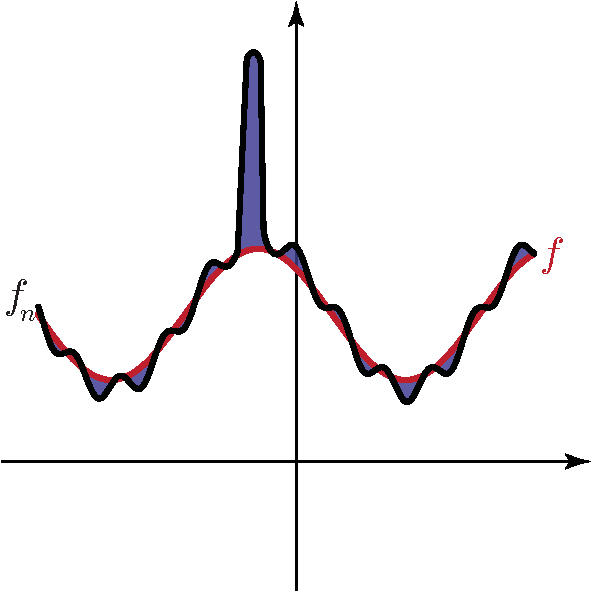
\includegraphics[trim=0cm 0cm 0cm 0cm, clip, scale=0.65]{images/visualizzazioneconvergenzal1.pdf}
\end{center}
Si nota che il grafico di $f_n$ può stare, in qualche zona, molto distante dal grafico di $f$, l'importante è che \textit{complessivamente} l'\textbf{area} tra $f_n$ e $f$ diminuisce, al crescere di $n$, fino ad essere \textit{nulla}.\\
Questa è la differenza principale tra la convergenza uniforme/puntuale/quasi ovunque e quella in $L^1$: se per le prime tre è fondamentale minimizzare la \textit{distanza} tra la funzione $f_n$ e $f$, l'ultima richiede di minimizzare l'\textit{area} tra le due.
\paragraph{Convergenza uniforme e in {$L^1$}}
\begin{theorema}[Legame tra convergenza uniforme e {$L^1$} nel caso di misura finita]
	Consideriamo lo spazio di misura $\left(X,\mathcal{M},\mu\right)$ e le funzione $\funz{f_n,f}{X}{\complexset}$. Se
	\begin{enumerate}[label=(\alph*)]
		\item $f_n\in L^{1}\left(\mu\right)$.
		\item $f_n$ converge uniformemente a $f$ su $X$.
		\item $\mu(X)<+\infty$.
	\end{enumerate}
	allora
	\begin{enumerate}
		\item $f\in L^{1}\left(\mu\right)$.
		\item $\displaystyle\lim_{n\to+\infty}\norm{f_n-f}_1=0$.
		\item Vale il \textbf{passaggio al limite sotto segno di integrale}\index{passaggio al limite sotto segno di integrale}
		\begin{equation}
			\lim_{n\to+\infty}\int_Xf_nd\mu=\int_Xfd\mu
		\end{equation}
	\end{enumerate}
\end{theorema}
\begin{demonstration}~{}
	\begin{enumerate}[label=(\Roman*)]
		\item Dobbiamo dimostrare che $f\in L^!\left(\mu\right)$, ovvero
		\begin{itemize}
			\item $f$ misurabile.
			\item $\displaystyle\int_X\abs{f}d\mu<+\infty$
		\end{itemize}
		Per ipotesi si ha la convergenza uniforme di $f_n$ a $f$ in $X$:
		\begin{equation*}
			\circled[red]{\vardiamond}\quad \forall \epsilon > 0,\ \exists N=N\left(\epsilon\right)\colon \forall n\geq N,\ \abs{f_n(x)-f(x)}<\epsilon,\ \forall x\in X
		\end{equation*}
		Osserviamo che $f$ è dunque misurabile, in quanto la misurabilità passa al limite puntuale (e quindi al limite uniforme). Da $\circled[red]{\vardiamond}$ segue che
		\begin{equation*}
			\abs{f(x)}\underset{=}{\forall n\in\naturalset}\abs{f(x)-f_n(x)+f_n(x)}\leq\abs{f(x)-f_n(x)}+\abs{f_n(x)}\underset{\forall x\in X}{<}\epsilon +\abs{f(x)}
		\end{equation*}
		Posto, ad esempio, $\epsilon = 1$ e $n=N$ si ha
		\begin{equation*}
			\abs{f(x)}=1+\abs{f_N(x)},\ \forall x\in X
		\end{equation*}
		Allora
		\begin{align*}
			\int_X\abs{f}d\mu&\leq \int_X \left(1+\abs{f_N}\right)d\mu&\text{(monotonia integrale per l''integranda)}\\
			&=\int_{X}1d\mu+\int_X\abs{f_N}d\mu&\text{(additività dell'integranda)}\\
			&=\mu(x)+\int_X\abs{f_N}d\mu <+\infty&
		\end{align*}
		perché $\mu(x)<+\infty$ per ipotesi e $f_n\in L^1\left(\mu\right)$.
		\item Dobbiamo dimostrare che $\displaystyle\lim_{n\to+\infty}\norm{f_n-f}_1=0$, ossia
		\begin{equation*}
			\circled[blue]{\spadesuit}\quad \forall \epsilon > 0,\ \exists \widetilde{N}=\widetilde{N}\left(\epsilon\right)\colon \forall n\geq N,\ \norm{f_n(x)-f(x)}_1<\epsilon
		\end{equation*}
		Si ha
		\begin{equation*}
			\norm{f_n-f}_1=\int_X\abs{f_n-f}d\mu\underset{\forall n\geq N\left(\epsilon\right)}{\overset{\circled[red]{\vardiamond}}{\leq}}\int_X\epsilon d\mu=\epsilon \mu(x)<+\infty
		\end{equation*}
		Vale la relazione \circled[blue]{\spadesuit} ponendo $\widetilde{N}=N$.
		\item Segue dal \textit{teorema di convergenza dominata}.
	\end{enumerate}
\end{demonstration}
\begin{attention}
	Se $\mu(x)=+\infty$, in generale \textit{non} vale nessuna delle tesi: come controesempi si possono prendere i tre esposti\footnote{Si veda \refChapterOnly{convergenzafunzioni}, pag. \pageref{controesempipassaggiointegrale}.} nel discorso sui problemi di integrabilità nell'ambito della teoria di Riemann.
\end{attention}
In generale non vale il viceversa: dalla convergenza $L^1$ non segue quella uniforme.
\begin{example}
	Consideriamo la successione
	\begin{equation*}
		f_n(x)=n\chi_{\left[0,\frac{1}{n^2}\right]}(x)=
		\begin{cases}
			\begin{array}{ll}
				n&0\leq x\leq\frac{1}{n^2}\\
				0&x< 0\vee x>\frac{1}{n^2}
			\end{array}
		\end{cases}
	\end{equation*}
	La successione converge in $L^1$ a $f\equiv 0$:
	\begin{equation*}
		\lim_{n\to+\infty}\norm{f_n-f}_1=\lim_{n\to+\infty}\int_{\realset}\abs{f_n-f}d\mu=\lim_{n\to+\infty}\int_{0}^{\frac{1}{n^2}}ndx=\lim_{n\to+\infty}n\cdot\frac{1}{n^2}=\lim_{n\to+\infty}\frac{1}{n}=0
	\end{equation*}
	Tuttavia, essa non converge uniformemente a $0$ su $\realset$, dato che
	\begin{equation*}
		\lim_{n\to+\infty}\left(\sup_{x\in\realset}\abs{f_n(x)-f(x)}\right)=\lim_{n\to+\infty}\left(\sup_{x\in\realset}\abs{n-0}\right)=+\infty\neq 0
	\end{equation*}
\end{example}
\begin{observe}
	Questo teorema ci mostra che il passaggio al limite sotto segno di integrale visto nell'ambito della teoria di Riemann, che contemplava la convergenza uniforme su intervalli limitati, è valido anche nell'ambito della Teoria di Lebesgue.
\end{observe}
Con questo teorema abbiamo finalmente risposto in toto ad uno dei quesiti inizialmente enunciati nel \refChapterOnly{ellipseintroduction}: nell'ambito della teoria di Lebesgue, ci sono tre differenti teoremi per il passaggio al limite sotto il segno di integrale, che sono quelli di
\begin{itemize}
	\item Convergenza uniforme su spazi di misura finita.
	\item Convergenza monotona.
	\item Convergenza dominata.
\end{itemize}
\paragraph{Convergenza in misura}
\begin{define}[Convergenza in misura]
	Consideriamo lo spazio di misura $\left(X,\mathcal{M},\mu\right)$ e le funzione $\funz{f_n,f}{X}{\complexset}$ misurabili per ogni $n$; $\forall n\in\naturalset$ definiamo la funzione $g_n\coloneqq \abs{f_n-f}$. Allora, se prendiamo $\forall n\in\ \naturalset,\forall \epsilon>0$ l'insieme
	\begin{equation*}
		E_{n,\epsilon}\coloneqq g^{-1}_n\left(\left(\epsilon,+\infty\right)\right)=\left\{x\in X\mid \abs{f_n(x)-f(x)}>\epsilon\right\}
	\end{equation*}
	si dice che	$f_n$ \textbf{converge in misura}\index{convergenza!in misura} a $f$ ($f_n\overset{\mu}{\to} f$) se
	\begin{equation}
		\lim_{n\to+\infty}\mu\left(\left\{x\in X\mid \abs{f_n(x)-f(x)}>\epsilon\right\}\right)=0,\ \forall \epsilon >0
	\end{equation}
\end{define}
Considerato $X\subseteq \realset$, possiamo visualizzare graficamente la convergenza in misura.
\begin{center}
	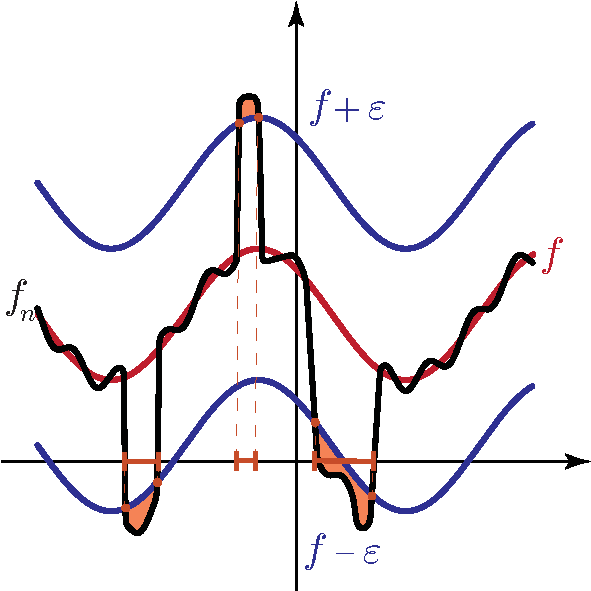
\includegraphics[trim=0cm 0cm 0cm 0cm, clip, scale=0.55]{images/visualizzazioneconvergenzamisura.pdf}
\end{center}
Possiamo interpretare questa convergenza come un particolare tipo di convergenza in $L^1$, condividendo però alcune caratteristiche con la convergenza \textit{uniforme} e alla convergenza \textit{quasi ovunque}. Arbitrariamente scelto un raggio $\epsilon$, il grafico di $f_n$ è nella quasi sua totalità contenuto nell'\textit{intorno tubulare} di raggio $\epsilon$ centrato sul grafico di $f$, ma è concesso che esso possa \textit{uscire} da tale intorno purché la misura dell'insieme di tutti i punti di $\realset$ in cui ciò accade tenda ad essere nulla al crescere di $n$.
\paragraph{Convergenza in {$L^1$} e in misura}
\begin{theorema}[Legame tra convergenza {$L^1$} e convergenza in misura]
	Consideriamo lo spazio di misura $\left(X,\mathcal{M},\mu\right)$ e le funzione $\funz{f_n,f}{X}{\complexset}$ tali che $f_n,f\in L^1\left(\mu\right)$.
	Allora
	\begin{equation}
		f_n\text{ converge in }L^1\text{ a }f\implies f_n\text{ converge in misura a }f
	\end{equation}
\end{theorema}
\begin{demonstration}
	Dobbiamo dimostrare che
	\begin{equation*}
		\mu\bigg(\underbrace{\left\{x\in X\middle|\abs{f_n(x)-f(x)}>\epsilon\right\}}_{\coloneqq E_{n,\epsilon}}\bigg)=0,\ \forall \epsilon>0
	\end{equation*}
	Si ha, per monotonia dell'integrale rispetto al dominio,
	\begin{equation*}
		\int_X\abs{f_n-f}d\mu\geq\int_{E_{n,\epsilon}}\abs{f_n-f}d\mu\geq\epsilon\int_{E_{n,\epsilon}}d\mu=\epsilon\mu\left(E_{n.,\epsilon}\right),\ \forall \epsilon>0,\ \forall n\geq 1
	\end{equation*}
	Dunque si ottiene
	\begin{equation*}
		0\leq \mu\left(E_{n,\epsilon}\right)\leq \frac{1}{\epsilon}\int_X\abs{f_n-f}d\mu=\frac{1}{\epsilon}\underbrace{\norm{f_n-f}_1}_{\substack{\to 0\text{ per }\\n\to+\infty}}
	\end{equation*}
	Passando al limite per $n\to+\infty$, applicando il \textit{teorema del confronto} si ricava:
	\begin{equation*}
		\lim_{n\to+\infty}\mu\left(E_{n,\epsilon}\right)=0,\ \forall \epsilon>0\qedhere
	\end{equation*}
\end{demonstration}
In generale non vale il viceversa: dalla convergenza in misura non segue la convergenza $L^1$.
\begin{example}
	Consideriamo la successione
	\begin{equation*}
		f_n(x)=n\chi_{\left[0,\frac{1}{n}\right]}(x)=
		\begin{cases}
			\begin{array}{ll}
				n&0\leq x\leq\frac{1}{n}\\
				0&x< 0\vee x>\frac{1}{n}
			\end{array}
		\end{cases}
	\end{equation*}
	La successione \textit{non} converge in $L^1$ a $f\equiv 0$:
	\begin{equation*}
		\lim_{n\to+\infty}\norm{f_n-f}_1=\lim_{n\to+\infty}\int_{\realset}\abs{f_n-f}d\mu=\lim_{n\to+\infty}\int_{0}^{\frac{1}{n}}ndx=\lim_{n\to+\infty}n\cdot\frac{1}{n}=\lim_{n\to+\infty}1=1\neq 0
	\end{equation*}
	Tuttavia, essa converge in misura a $0$ su $\realset$, dato che
	\begin{align*}
		&\left\{x\in X\mid \abs{f_n(x)-f(x)}>\epsilon\right\}=\left\{x\in X\mid \abs{f_n(x)}>\epsilon\right\}=\left[0,n\right],\ \forall \epsilon>0\\
		&\implies\lim_{n\to+\infty}\mu\left(\left\{x\in X\mid \abs{f_n(x)-f(x)}>\epsilon\right\}\right)=\lim_{n\to+\infty}\mu\left(\left[0,\frac{1}{n}\right]\right)=\lim_{n\to+\infty}\frac{1}{n}=0,\ \forall \epsilon >0
	\end{align*}
\end{example}
%% SVN info for this file
\svnidlong
{$HeadURL$}
{$LastChangedDate$}
{$LastChangedRevision$}
{$LastChangedBy$}

\chapter{Integrali dipendenti da un parametro}
\labelChapter{integralidipendentiparametro}

\begin{introduction}
	‘‘La matematica confronta i più disparati fenomeni e scopre le analogie segrete che li uniscono.''
	\begin{flushright}
		\textsc{Joseph Fourier,} cercando disperatamente di motivare ai suoi genitori la scelta di studiare matematica.
	\end{flushright}
\end{introduction}
\lettrine[findent=1pt, nindent=0pt]{S}{tudieremo} \textbf{[COMPLETARE]}
% TO DO: completare intro
\section{Integrali dipendenti da un parametro}
Nel corso di \textsc{Analisi Matematica 2} abbiamo incontrato gli \textit{integrali dipendenti da un parametro} nella teoria dell'integrazione di Riemann. Espandiamo questo argomento agli integrali di Lebesgue.
\begin{define}[Integrali dipendenti da un parametro]
	Consideriamo lo spazio di misura $\left(\realset,\mathcal{L}\left(\realset\right),m_1\right)$. Un \textbf{integrale dipendente da un parametro}\index{integrale!dipendente da un parametro} è una funzione
	\begin{equation}
		F(t)=\int_I\mvf{f}{t}{x}dm_1(x),\ \forall t\in J
	\end{equation}
	dove $I,J$ sono intervalli in $\realset$ e
	\begin{equation*}
		\funztot{f}{I\times J}{\complexset}{\left(t,x\right)}{\mvf{f}{t}{x}}
	\end{equation*}
	è tale per cui $\forall t\in I\ \funz{f\left(t,\cdot\right)}{J}{\complexset}$ integrabile.
\end{define}
Vogliamo studiare le proprietà di continuità e derivabilità dell'integrale dipendente da una parametro a partire da quelle della funzione $f$ che lo definisce.
\begin{theorema}[Teorema di continuità e derivabilità di integrali dipendenti da un parametro]
	Siano $I,J\subseteq\realset$ intervalli e sia $\funz{f}{I\times J}{\complexset}$ tale che $f\left(t,\cdot\right)$ sia integrabile, $\forall t\in I$. Consideriamo
	\begin{equation*}
		F(t)=\int_I\mvf{f}{t}{x}dm_1(x)
	\end{equation*}
	\begin{enumerate}
		\item Se
		\begin{itemize}
			\item $f\left(\cdot, x\right)$ è continua su $I$, $\forall x\in J$.
			\item $\exists \funz{\phi}{I}{\realset}$ integrabile tale che
			\begin{equation*}
				\abs{\mvf{f}{t}{x}}\leq\phi(x),\ \forall \left(t,x\right)\in I\times J
			\end{equation*}
		\end{itemize}
		allora $F$ è continua su $I$.
		\item Se
		\begin{itemize}
			\item $\exists\frac{\partial f}{\partial t}$ su $I\times J$.
			\item $\exists\funz{\psi}{J}{\realset}$ integrabile tale che
			\begin{equation*}
				\abs{\frac{\partial f}{\partial t}\left(t,x\right)}\leq\psi(x),\ \forall \left(t,x\right)\in I\times J
			\end{equation*}
			allora $F$ è continua su $I$ e si ha la \textbf{derivazione sotto segno di integrale}\index{derivazione sotto segno di integrale}:
			\begin{equation*}
				F'(t)=\int_J\frac{\partial f}{\partial t}\left(t,x\right)dm_1(x), \forall t\in I
			\end{equation*}
		\end{itemize}
	\end{enumerate}
\end{theorema}
Per dimostrare questo teorema ci serviranno i seguenti fatti:
\begin{itemize}
	\item \textbf{Teorema di relazione:} data $\funz{g}{I\subseteq\realset}{\complexset}$ e $\overline{t}\in I$, si ha
	\begin{equation}
		\lim_{t\to\overline{t}}g(t)=L\in\complexset\iff\lim_{n\to+\infty}g\left(t_n\right)=L,\ \forall t_n\to\overline{t}
	\end{equation}
	\item \textbf{Teorema di Lagrange:} data $\funz{g}{I\subseteq\realset}{\complexset}$ derivabile su $I$, si ha
	\begin{equation}
		\forall t_1,t_2\in I, \abs{g\left(t_1\right)-g\left(t_2\right)}\leq\sup_{t\in\left[t_1,t_2\right]}\abs{g'(t)}\abs{t_1-t_2}
	\end{equation}
\end{itemize}
\begin{demonstrationcaputwt}[della continuità e derivabilità di {$F$}]
	\begin{enumerate}[label=\Roman*]
		\item Dobbiamo provare che
		\begin{equation*}
			\forall \overline{t}\in I,\ \lim_{t\to\overline{t}}F(t)=F\left(\overline{t}\right)
		\end{equation*}
		È sufficiente provare che, per il primo fatto enunciato precedentemente,
		\begin{equation*}
			\forall \overline{t}\in I,\ \forall t_n\to\overline{t}, \lim_{n\to+\infty}F\left(t_n\right)=F\left(\overline{t}\right)
		\end{equation*}
		Siano quindi $\overline{t}\in I$ e $t_n\to\overline{t}$ fissati: dobbiamo provare che
		\begin{equation*}
			\lim_{n\to+\infty}\int_Jf\left(t_n,x\right)dm_1(x)=\int_Jf\left(\overline{t},x\right)dm_1(x)
		\end{equation*}
		Ponendo
		\begin{align*}
			g_n(x)\coloneqq f\left(t_n,x\right)\\
			\overline{g}(x)\coloneqq f\left(\overline{t},x\right)
		\end{align*}
		allora la relazione da provare si scrive come
		\begin{equation*}
			\lim_{n\to+\infty}\int_Jg_n(x)dm_1(x)=\int_J\overline{g}(x)dm_1(x)
		\end{equation*}
		ossia ho ottenuto un problema di passaggio al limite sotto segno di integrale. Applichiamo il teorema di convergenza dominata, verificandone le ipotesi:
		\begin{itemize}
			\item \textbf{Convergenza puntuale:}
			\begin{equation*}
				\forall x\in J,\ \lim_{n\to+\infty}g_n(x)=\lim_{n\to+\infty}f\left(t_n,x\right)=f\left(\overline{t},x\right)=\overline{g}(x)
			\end{equation*}
			perché $f\left(\cdot,x\right)$ è continua rispetto alla $t$.
			\item \textbf{Maggiorazione (convergenza dominata):}
			\begin{equation*}
				\abs{g_n(x)}\underset{\substack{\forall n\geq 1\\\forall x\in J}}{=}\abs{f\left(t_n,x\right)}\leq \phi(x)\quad\text{(indipendentemente da $n$)}
			\end{equation*}
		\end{itemize}
		Si può allora passare al limite sotto segno di integrale e concludere.
		\item Dobbiamo provare che
		\begin{equation*}
			F'(t)=\int_J\frac{\partial f}{\partial t}\left(\overline{t},x\right)dm_1(x),\ \forall \overline{t}\in I
		\end{equation*}
		ossia
		\begin{equation*}
			\lim_{t\to\overline{t}}\frac{F(t)-F\left(\overline{t}\right)}{t-\overline{t}}=\int_J\frac{\partial f}{\partial t}\left(\overline{t},x\right)dm_1(x),\ \forall \overline{t}\in I
		\end{equation*}
		Per il primo dei fatti è sufficiente provare che
		\begin{equation*}
			\lim_{n\to+\infty}\frac{F\left(t_n\right)-F\left(\overline{t}\right)}{t_n-\overline{t}}=\int_J\frac{\partial f}{\partial t}\left(\overline{t},x\right)dm_1(x),\ \forall \overline{t}\in I,\ \forall t_n\to \overline{t}
		\end{equation*}
		Siano allora $\overline{t}\in I$ e $t_n\to\overline{t}$ fissati: dobbiamo provare che
		\begin{align*}
			\lim_{n\to+\infty}\frac{F\left(t_n\right)-F\left(\overline{t}\right)}{t_n-\overline{t}}&=\lim_{n\to+\infty}\frac{1}{t_n-\overline{t}}\left(\int_Jf\left(+t_n,x\right)dm_1(x)-\int_Jf\left(\overline{t},x_n\right)dm_1(x)\right)=\\
			&=\lim_{n\to+\infty}\int_J\underbrace{\frac{f\left(t_n,x\right)-f\left(\overline{t},x\right)}{t_n-\overline{t}}}_{\coloneqq h_n(x)}dm_1(x)=\int_J\underbrace{\frac{\partial f}{\partial t}\left(\overline{t},x\right)}_{\coloneqq \overline{h}(x)}dm_1(x)
		\end{align*}
		ottenendo
		\begin{equation*}
			\lim_{n\to+\infty}\int_Jh_n(x)dm_1(x)=\int_J\overline{h}(x)dm_1(x)
		\end{equation*}
		ossia ho di nuovo un problema di passaggio al limite sotto segno di integrale. Come prima, applichiamo il teorema di convergenza dominata, verificandone le ipotesi:
		\begin{itemize}
			\item \textbf{Convergenza puntuale:}
			\begin{equation*}
				\forall x\in J,\ \lim_{n\to+\infty}h_n(x)=\overline{h}(x)
			\end{equation*}
			per definizione di derivata parziale.
			\item \textbf{Maggiorazione (convergenza dominata):}
			\begin{equation*}
				\abs{h_n(x)}\underset{\substack{\forall n\geq 1\\\forall x\in J}}{=}\abs{\frac{f\left(t_n,x\right)-f\left(\overline{t},x\right)}{t_n-t}}\underset{\text{fatto }2}{\leq} \frac{\displaystyle\sup_{t\in\left[t_n,\overline{t}\right]}\abs{\frac{\partial f}{\partial t}}\Ccancel[red]{\abs{t_n-\overline{t}}}}{\Ccancel[red]{\abs{t_n-\overline{t}}}}\leq \psi(x)
			\end{equation*}
		\end{itemize}
		Si può allora passare al limite sotto segno di integrale e concludere.\qedhere
	\end{enumerate}
\end{demonstrationcaputwt}
\section{La trasformata di Fourier}
\begin{define}[Trasformata di Fourier]
	Sia $\funz{g}{\realset}{\realset}$. Data la funzione
	\begin{equation*}
		\mvf{f}{t}{x}=g(x)e^{-itx},\ \forall \left(t,x\right)\in\realset^2,
	\end{equation*}
	dove
	\begin{equation*}
		e^{-itx}=\cos tx-i\sin tx,\ \forall\left(t,x\right)\in\realset^2,
	\end{equation*}
	definiamo la \textbf{trasformata di Fourier}\index{trasformata di Fourier} di $g$ l'integrale dipendente dal parametro di $t$ dato da $f$:
	\begin{equation}
		\begin{array}{ll}
			\displaystyle\hat{g}(t)&=\displaystyle\int_{\realset}g(x)e^{-itx}dm_1(x)=\\
			&=\displaystyle\int_{\realset}g(x)\cos txdm_1(x)-i\int_\realset g(x)\sin txdm_1(x),\ \forall t\in\realset
		\end{array}
	\end{equation}
\end{define}
Ci chiediamo sotto quali ipotesi su $g$ la funzione $F$ è continua e sotto quali invece è derivabile.
\begin{theorema}[Continuità e derivabilità della trasformata di Fourier]
	Sia data $\funz{g}{\realset}{\realset}$.
	\begin{enumerate}
		\item Se $g\in L^1\left(\realset\right)$, allora $\hat{g}$ è continua su $\realset$.
		\item Se
		\begin{itemize}
			\item $g\in L^1\left(\realset\right)$.
			\item $xg(x)\in L^1\left(\realset\right)$.
		\end{itemize}
		allora $\hat{g}$ è derivabile su $\realset$ e
		\begin{equation}
			\hat{g}'(t)=\widehat{\left(-ixg(x)\right)}=-i\int_{\realset}xg(x)e^{-itx}dm_1(x),\ \forall t\in\realset
		\end{equation}
	\end{enumerate}
\end{theorema}
\begin{demonstration}~
	\begin{enumerate}[label=\Roman*]
		\item % TO DO: completare
		\item Applichiamo il teorema di derivabilità degli integrali dipendenti da un parametro. In questo caso si ha
		\begin{equation*}
			\mvf{f}{t}{x}=g(x)e^{-itx},\ \forall \left(t,x\right)\in\realset^2
		\end{equation*}
		Verifichiamo le ipotesi.
		\begin{itemize}
			\item $\mvf{f}{t}{\cdot}$ è integrabile su $\realset$:
			\begin{itemize}
				\item $\mvf{f}{t}{\cdot}$ misurabile perché $f$ è il prodotto di $g$ e $e^{-itx}$, due funzioni misurabili - la prima per ipotesi, la seconda in quanto è continua.
				\item $\displaystyle\int_{\realset}\abs{\mvf{f}{t}{x}}<+\infty$ in quanto
				\begin{equation*}
					\abs{\mvf{f}{t}{x}}=-ixg(x)e^{-itx},\ \forall \left(t,x\right)\in\realset^2
				\end{equation*}
			\end{itemize}
			\item Esiste
			\begin{equation*}
				\frac{\partial f}{\partial t}=-ixg(x)e^{itx},\ \forall \left(t,x\right)\in\realset^2
			\end{equation*}
			\item Si può maggiorare uniformemente $\dfrac{\partial f}{\partial t}$ in $t$ con una funzione integrabile:
			\begin{equation*}
				\abs{\frac{\partial f}{\partial t}\left(t,x\right)}=\abs{-ixg(x)e^{-itx}}=\abs{xg(x)}\underbrace{\abs{e^{-itx}}}_{=1}=\abs{xg(x)}\coloneqq \psi(x),\ \forall \left(t,x\right)\in\realset^2
			\end{equation*}
			con $\psi(x)$ integrabile per ipotesi sull'integrabilità di $xg(x)$.
		\end{itemize}
		Ne segue che $\hat{g}$ è derivabile e
		\begin{equation*}
			\hat{g}'(t)=\int_{\realset}\frac{\partial f}{\partial t}\left(t,x\right)dm_1(x)=-i\int_{\realset}xg(x)e^{-itx}dm_1(x)\qedhere
		\end{equation*}
	\end{enumerate}
\end{demonstration}
%\part{Classificazione delle superfici topologiche}
%\labelPart{third}
%% SVN info for this file
\svnidlong
{$HeadURL$}
{$LastChangedDate$}
{$LastChangedRevision$}
{$LastChangedBy$}

\chapter{Analisi e probabilità}
\labelChapter{analisiprobabilità}

\begin{introduction}
	‘‘Se il tuo esperimento richiede di usare la statistica, dovevi fare un esperimento migliore.''
	\begin{flushright}
		\textsc{Ernest Rutherford,} stanco di studiare Calcolo delle Probabilità e Statistica.
	\end{flushright}
\end{introduction}
\lettrine[findent=1pt, nindent=0pt]{C}{ome} abbiamo potuto notare nel corso di \textsc{Calcolo di Probabilità}, la teoria della \textbf{probabilità} si è notevolmente espansa dal mero studio di eventi discreti con metodi combinatoriali. Infatti, Andrey Nikolaevich \textbf{Kolmogorov} (1903 – 1987) nel 1933 combinò la nozione di spazio campione, già introdotta da Richard \textbf{von Mises} (1883 – 1953), e la teoria della misura di Lebesgue per definire un sistema assiomatico compatibile sia con la teoria \textit{classica} della probabilità, sia con l'\textit{Analisi moderna}: in questo modo, gli eventi potevano essere anche un qualcosa di \textit{continuo}, con tutto ciò che ne consegue.\\
In questo ultimo capitolo di teoria approfondiremo alcuni concetti visti a \textsc{Calcolo di Probabilità} con il formalismo e il rigore dato dalla teoria della Misura e dell'integrazione. Partiremo con l'enunciare gli \textit{assiomi di probabilità} di Kolmogorov per poi dedicarci a come studiare le \textit{variabili aleatorie} tramite la sola \textit{probabilità immagine}, e in base ad essa dare una classificazione \textit{esaustiva} delle variabili aleatorie. Concludiamo la trattazione rivedendo i \textit{modi di convergenza} delle funzioni misurabili in ambito probabilistico.
\section{Spazio di probabilità e variabili aleatorie}
\begin{define}[Spazio di probabilità]
	Uno \textbf{spazio di probabilità}\index{spazio!di probabilità} $\left(\Omega,\mathcal{F},\mathbb{P}\right)$ è una struttura matematica che fornisce un modello formale per un esperimento non deterministico. Essa costituita dai seguenti elementi:
	\begin{enumerate}
		\item Uno \textbf{spazio campionario}\index{spazio!campionario} $\Omega$, l'insieme di tutti i possibili \textbf{risultati} $\omega$ dell'esperimento.
		\item Uno \textbf{spazio degli eventi}\index{spazio!degli eventi} $\mathcal{F}$, la famiglia di tutti gli eventi dell'esperimento, dove un \textbf{evento}\index{evento} $E$ è un insieme di risultati dello spazio campionario - ossia un sottoinsieme di $\Omega$.
		\item Una \textbf{funzione di probabilità} $\mathbb{P}$, che assegna ad ogni evento una probabilità, la quale è un numero tra 0 e 1.
		\begin{equation}
			\funz{\mathbb{P}}{\mathcal{F}}{\left[0,1\right]}
		\end{equation}
	\end{enumerate}
\end{define}
Questo spazio di probabilità deve soddisfare gli assiomi di probabilità introdotti da Andrey Kolmogorov nel 1933.
\begin{axiom}[Primo assioma di probabilità]
	La probabilità di un evento è un numero reale non negativo.
	\begin{equation}
		\mathbb{P}\left(E\right)\in\realset,\ \mathbb{P}\left(E\right)\geq 0\quad \forall E\in\mathcal{F} 
	\end{equation}
\end{axiom}
\begin{axiom}[Secondo assioma di probabilità]
	La probabilità dello spazio campionario è $1$.
	\begin{equation}
		\mathbb{P}\left(\Omega\right)=1
	\end{equation}
\end{axiom}
\begin{axiom}[Terzo assioma della probabilità]
	La probabilità è $\sigma$-additiva:	$\forall A_n\in\mathcal{F}$ tali che $A_i\cap A_j=\emptyset\ \forall i\neq j$, allora
	\begin{equation}
		\mathbb{P}\left(\coprod_{n\geq 1}A_n\right)=\sum_{n\geq 1}\mathbb{P}\left(A_n\right)
	\end{equation}
\end{axiom}
\begin{proposition}[L'insieme vuoto ha probabilità nulla]
	Sia $\left(\Omega,\mathcal{F},\mathbb{P}\right)$ uno spazio di probabilità. Allora l'insieme vuoto ha probabilità nulla.
\end{proposition}
\begin{demonstration}
	Consideriamo la successione di eventi seguente:
	\begin{equation*}
		A_n=\begin{cases}
			\begin{array}{ll}
				\Omega&n=1\\
				\emptyset&n\geq2
			\end{array}
		\end{cases}
	\end{equation*}
	Osserviamo che $\Omega\cap \emptyset=\emptyset$ e $\emptyset\cap\emptyset=0$; poiché
	\begin{equation*}
		\Omega=\bigcup_{n\geq 1}A_n,
	\end{equation*}
	applichiamo l'assioma 3, la $\sigma$-additività all'unione degli $A_n$:
	\begin{align*}
		1&=\mathcal{P}\left(\Omega\right)=\mathcal{P}\left(\bigcup_{n\geq 0}A_n\right)=\sum_{n\geq 1}\mathbb{P}\left(A_n\right)=\mathbb{P}\left(A_1\right)+\sum_{n\geq2}\mathbb{P}\left(A_n\right)&\\
		&=\mathbb{P}\left(\Omega\right)+\sum_{n\geq 2}\mathbb{P}\left(\emptyset\right)&\text{(Assioma 1)}\\
		&=1-\sum_{n\geq 2}\mathbb{P}\left(\emptyset\right)&
	\end{align*}
	da cui
	\begin{equation*}
		\sum_{n\geq 2}\mathbb{P}\left(\emptyset\right)=0
	\end{equation*}
	Poiché per il primo assioma la probabilità di un evento è sempre non-negativa, ne consegue che ogni elemento di questa sommatoria debba essere uguale a zero, ossia $\mathcal{P}\left(\emptyset\right)=0$.
\end{demonstration}
Si può subito osservare che lo spazio di probabilità $\left(\Omega,\mathcal{F},\mathbb{P}\right)$ altro non è che uno \textbf{spazio di misura} $\left(X,\mathcal{M},\mu\right)$, con l'ipotesi aggiunta che la misura $\mu$ sia di \textbf{probabilità}, cioè $\mu(X)=1$.
\begin{define}[Funzione misurabile]
	Sia $\left(\Omega,\mathcal{F},\mathbb{P}\right)$ uno spazio di probabilità. Una funzione $\funz{X}{\Omega}{\complexset}$ si dice \textbf{variabile aleatoria}\index{variabile aleatoria} se \begin{equation}
		X^{-1}\left(A\right)\in\mathcal{F},\ \forall A\subseteq \complexset\text{ aperto.}
	\end{equation}
\end{define}
In altre parole, una variabile aleatoria è una funzione misurabile da uno spazio di probabilità a $\complexset$.
\section{Probabilità immagine}\label{probimm}
Nel corso di \textsc{Calcolo di Probabilità} abbiamo incontrato la variabile aleatoria \textbf{normale standard} $Z$, definita come tale se la probabilità che $Z$ stia nell'evento $B$ è
\begin{equation}
	\mathbb{P}\left(Z\in B\right)=\int_{B}\frac{1}{\sqrt{2\pi}}e^{-x^2/2}dm_1,\ \forall B\in\mathcal{B}\left(\realset\right)
\end{equation}
Le variabili aleatorie, per definizione, sono funzioni da uno spazio di probabilità $\Omega$ a valori - in questo caso - reali. La definizione della normale standard, tuttavia, non fa alcun riferimento allo spazio di probabilità. Cos'è dunque  $\left(\Omega,\mathcal{F},\mathbb{P}\right)$?\\
In realtà \textit{non si sa}, ma non ci interessa individuarlo. Motiviamo questa affermazione audace introducendo il concetto di \textit{misura immagine}, visto nell'ambito di Teoria della probabilità come \textit{probabilità immagine}.
\begin{define}[Misura immagine]
	Siano $\left(X,\mathcal{F}\right)$ e $\left(Y,\mathcal{M}\right)$ due spazi misurabili e una funzione $\funz{f}{X}{Y}$ misurabile. Se su $\left(X,\mathcal{F}\right)$ consideriamo una misura $\funz{\mu}{\mathcal{F}}{\left[0,+\infty\right]}$, la \textbf{misura immagine}\index{misura!immagine} o \textbf{pushforward}\index{misura!pushforward} è la misura $\funz{f_{\ast}\left(\mu\right)}{\mathcal{M}}{\left[0,+\infty\right]}$ definita da
	\begin{equation}
		\left[f_{\ast}\left(\mu\right)\right]\left(B\right)=\mu\left(f^{-1}\left(B\right)\right),\ \forall B\in \mathcal{M}
	\end{equation}
\end{define}
\begin{theoremaqed}[Integrazione con cambio di variabili tramite pushforward]
	Data una funzione $g$ su $Y$ misurabile, allora
	\begin{equation}
		g\in L^{1}\left(f_{\ast}\left(\mu\right)\right)\iff g\circ f\in L^{1}\left(\mu\right),
	\end{equation}
	ossia
	\begin{equation}
		\int_{X}g\circ fd\mu=\int_{Y}gd\left(f_{\ast}\left(\mu\right)\right)\qedhere
	\end{equation}
\end{theoremaqed}
Interpretiamo questo nuovo concetto nell'ambito degli spazi di probabilità.
\begin{define}[Probabilità immagine]
	Sia $\left(X,\mathcal{M},\mathbb{P}\right)$ e spazio di probabilità e $\funz{X}{\Omega}{\realset}$ variabile aleatoria.
	La \textbf{probabilità immagine}\index{probabilità!immagine} è la misura di probabilità $\funz{\mathbb{P}_X}{\mathcal{B}\left(\realset\right)}{\left[0,1\right]}$ definita da
	\begin{equation}
		\mathbb{P}_X\left(B\right)=\mathbb{P}\left(X^{-1}\left(B\right)\right),\ \forall B\in \mathcal{B\left(\realset\right)}
	\end{equation}
	e definisce un nuovo spazio di probabilità $\left(\realset,\mathcal{B}\left(\realset\right),\mathbb{P}_X\right)$.
\end{define}
\begin{theoremaqed}[Integrazione con cambio di variabili tramite probabilità immagine]
	Data una funzione $g$ su $\realset$ misurabile, allora
	\begin{equation}
		\circled[blue]{\spadesuit}\quad g\in L^{1}\left(\mathbb{P}_X\right)\iff g\circ X\in L^{1}\left(\mathbb{P}\right),
	\end{equation}
	ossia
	\begin{equation}
		\int_{\Omega}g(x)d\mathbb{P}=\int_{\realset}gd\mathbb{P}_X\qedhere
	\end{equation}
\end{theoremaqed}
\begin{center}
	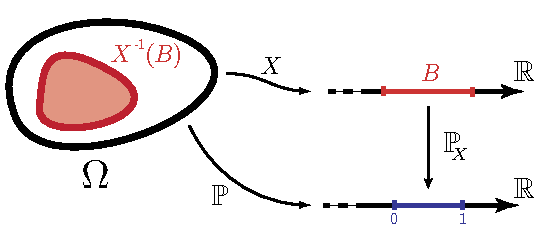
\includegraphics[width=0.4\paperwidth]{images/probimmagine}
\end{center}
Pertanto, non mi interessa nello specifico sapere cos'è $\Omega$ o com'è definita $\mathbb{P}$: se definisco la variabile aleatoria direttamente con la probabilità immagine ‘‘dimentico'' quale fosse lo spazio originale e lavoro direttamente su $\realset$.
\begin{define}[Momento di ordine {$k$-esimo}]
	Se consideriamo la funzione $g(x)=x^k,\ \forall x\in\realset$ e $\forall k\in\naturalset$, si definisce il \textbf{momento}\index{momento di ordine {$k$}-esimo} il valore
	\begin{equation*}
		\mathbb{E}\left(X^k\right)=\int_{\Omega}X^kd\mathbb{P}=\int_{\realset}x^kd\mathbb{P}_X
	\end{equation*}
\end{define}
\section{Funzione di ripartizione e classificazione delle variabili aleatorie}
\begin{define}[Funzione di ripartizione]
	Siano $\left(\Omega,\mathcal{M},\mathbb{P}\right)$ uno spazio di probabilità, $\funz{X}{\Omega}{\realset}$ una variabile aleatoria e $\mathbb{P}_X$ la corrispondente probabilità immagine. Si chiama \textbf{funzione di ripartizione}\index{funzione!di ripartizione} (abbreviata in \textbf{cdf}, dall'inglese \textit{cumulative distributive function}) la funzione $\funz{F_X}{\realset}{\left[0,1\right]}$ definita da
	\begin{equation}
		F_X(x)=\mathbb{P}_X\left(\left(-\infty,x\right]\right)=\mathbb{P}\left(X\leq x\right),\ \forall x\in\realset
	\end{equation}
\end{define}
Una funzione di ripartizione $F_X$ soddisfa le seguenti proprietà:
\begin{enumerate}
	\item È monotona non decrescente.
	\item È continua a destra.
	\item È tale per cui
	\begin{equation}
		\lim_{x\to+\infty}F_X(x)=0\quad\lim_{x\to+\infty}F_X(x)=1
	\end{equation}
	ossia ha immagine $\left[0,1\right]$.
\end{enumerate}
Vale anche il viceversa: una funzione che soddisfa queste caratteristiche è una funzione di ripartizione per qualche variabile aleatoria.\\
La variabili aleatorie si classificano in base alla probabilità immagine $\mathbb{P}_X$ e, di conseguenza, alla funzione di ripartizione $F_X$, in una delle quattro classi seguenti:
\begin{itemize}
	\item V.a. \textit{assolutamente continue}.
	\item V.a. \textit{singolari discrete}.
	\item V.a. \textit{singolari continue}.
	\item V.a. \textit{miste}.
\end{itemize}
\subsection{Variabili aleatorie assolutamente continue}
\begin{define}[V.a. assolutamente continua e densità]
	$X$ si dice variabile aleatoria \textbf{assolutamente continua}\index{variabile aleatoria!assolutamente continua} se $\mathbb{P}_X$ è assolutamente continua rispetto alla misura di Lebesgue $m_1$:
	\begin{equation}
		\forall E\in\mathcal{B}\left(\realset\right),\ m_1\left(E\right)=0\implies \mathbb{P}_X\left(E\right)=0
	\end{equation}
	Per il \textit{teorema di Radon-Nikodym} esiste quindi una funzione detta \textbf{densità} $f\in\mathcal{L}^1\left(\realset\right)$, $f\geq 0$ tale che
	\begin{equation}
		\mathbb{P}_X\left(B\right)=\int_B fdm_1,\ \forall B\in\mathcal{B}\left(\realset\right)
	\end{equation}
\end{define}
Abbiamo già visto\footnote{Si veda \refChapterOnly{integraledilebesgue}, pag. \pageref{misuraindotta}.} come integrare delle funzioni rispetto ad una misura indotta da un'altra misura, come qui è il caso.
\begin{theoremaqed}[Integrazione di funzioni rispetto a v.a. assolutamente continue]
	Data una funzione $g$ su $\realset$, allora
	\begin{equation}
		g\in L^{1}\left(\mathbb{P}_X\right)\iff fg\in L^{1}\left(m_1\right),
	\end{equation}
	ossia
	\begin{equation}
		\int_{\realset}gd\mathbb{P}_X=\int_{\realset}fgdm_1\qedhere
	\end{equation}
\end{theoremaqed}
\begin{define}[Momento di una ordine {$k$-esimo} di v.a. assolutamente continue]
	Sia $X$ una v.a. assolutamente continua di densità $f$. Se consideriamo la funzione $g(x)=x^k,\ \forall x\in\realset$ e $\forall k\in\naturalset$, si definisce il \textbf{momento}\index{momento di ordine {$k$}-esimo} il valore
	\begin{equation*}
		\mathbb{E}\left(X^k\right)=\int_{\Omega}X^kd\mathbb{P}=\int_{\realset}x^kd\mathbb{P}_X=\int_{\realset}x^kd\mathbb{P}_X=\int_{\realset}x^kfdm_1
	\end{equation*}
\end{define}
\begin{examplewt}[Variabile aleatoria normale]
	Approfondendo ciò ad inizio della sezione \ref{probimm}. La variabile aleatoria \textbf{normale standard}\index{variabile aleatoria!normale standard} è una variabile aleatoria $\funz{Z}{\Omega}{\realset}$ di cui è ignoto lo spazio di probabilità $\left(\Omega,\mathcal{M},\mathbb{P}\right)$; tuttavia, essa è definita attraverso la probabilità immagine $\mathbb{P}_X$ assolutamente continua rispetto alla misura $m_1$ associata alla densità Gaussiana:
	\begin{equation}
		\mathbb{P}\left(X\in\mathbb{B}\right)=\mathbb{P}_X\left(B\right)=\int_B\frac{1}{\sqrt{2\pi}}e^{-x^2/2}dm_1,\ \forall B\in\mathcal{B}\left(\realset\right)
	\end{equation}
	I momenti della v.a. normale standard sono
	\begin{equation*}
		\mathbb{E}X^k=\int_{\Omega}X^kd\mathbb{P}=\int_{\realset}x^kd\mathbb{P}_X=\int_{\realset}x^k\frac{1}{\sqrt{2\pi}}e^{-x^2/2}dm_1
	\end{equation*}
\end{examplewt}
\paragraph{Cdf di v.a. assolutamente continue}
La funzione di ripartizione $\funz{F_X}{\realset}{\left[0,1\right]}$ di una variabile aleatoria assolutamente continua è una funzione \textbf{assolutamente continua}.
\begin{center}
	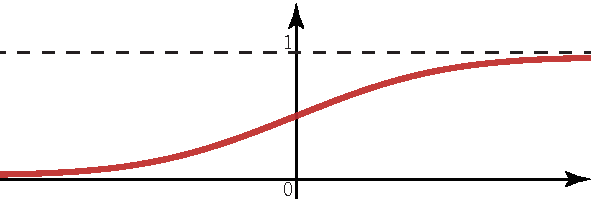
\includegraphics[width=0.4\paperwidth]{images/vacontinua}
\end{center}
\begin{define}[Assoluta continuità.]
	Una funzione $\funz{f}{\realset}{\realset}$ è assolutamente continua se
	\begin{gather*}
		\forall \epsilon>0,\ \exists \delta >0\colon \forall \left(a_1,b_1\right),\ \dots,\ \left(a_n,b_n\right),\ \left(a_i,b_i\right)\cap\left(a_j,b_j\right)=\emptyset,\ \forall i\neq j,\\
		\sum_{i=1}^{n}\abs{b_i-a_i}<\delta\implies\sum_{i=1}^{n}\abs{f\left(b_i\right)-f\left(a_i\right)}<\epsilon
	\end{gather*}
\end{define}
\begin{observe}
	Scegliendo un unico intervallo $\left(a_1,b_1\right)$ si ritrova la definizione di \textit{uniforme continuità}. Pertanto, l'assoluta continuità è una condizione più forte dell'uniforme continuità e in quanto tale implica anche la continuità della funzione originale.
\end{observe}
Ricordiamo che
\begin{equation*}
	F_X(x)=\mathbb{P}_X\left(\left(-\infty,x\right]\right)=\int_{\left(-\infty,x\right]}fdm_1
\end{equation*}
Si dimostra che $F_X$ è derivabile \textbf{q.o.} e che vale
\begin{equation}
	F'_X(x)=f(x),\ \textrm{per quasi ogni }x\in\realset
\end{equation}
Questa relazione non è altro che l'\textbf{estensione del teorema fondamentale del calcolo integrale alla teoria di Lebesgue}\index{teorema!fondamentale del calcolo integrale nella teoria di Lebesgue}.
\subsection{Misure singolari}
Consideriamo una misura $\funz{\lambda}{\mathcal{B}\left(\realset\right)}{\left[0,+\infty\right]}$ non assolutamente continua rispetto alla misura di Lebesgue $m_1$.
Negare
\begin{equation*}
	\forall E\in\mathcal{B}\left(\realset\right)\colon m_1\left(E\right)=0\implies \lambda\left(E\right)=0
\end{equation*}
significa che esiste un insieme $S\in\mathcal{B}\left(\realset\right)$ tale che
\begin{equation*}
	m_1\left(S\right)=0\text{ ma }\lambda\left(S\right)\neq 0
\end{equation*}
In particolare, se vale
\begin{equation*}
	\lambda\left(S\right)=\lambda\left(\realset\right)
\end{equation*}
la misura viene chiamata \textit{singolare} e si definisce \textit{concentrata} in $S$
\begin{define}[Misura singolare]
	Dato un spazio di misura $\left(X,\mathcal{M},\mu\right)$, una misura $\funz{\lambda}{\mathcal{M}}{\left[0,+\infty\right]}$ non assolutamente continua rispetto a $\mu$ si dice \textbf{singolare}\index{misura!singolare} rispetto a $\mu$ se
	\begin{equation}
		\exists S\in\mathcal{M}\colon \mu\left(S\right)=0, \lambda\left(S\right)\neq0 \text{ ma }\lambda(X)=\lambda\left(S\right)
	\end{equation}
	La misura $\lambda$ è detta \textbf{concentrata} in $S$ e si indica con $\mu\perp\lambda$.
	\begin{itemize}
		\item Se $\lambda$ è concentrata in $S$ insieme numerabile, allora $\lambda$ è detta \textbf{singolare discreta}\index{misura!singolare!discreta} o \textbf{atomica}\seeonlyindex{misura!singolare!atomica}{misura!singolare!discreta}.
		\item Se $\lambda$ è concentrata in $S$ insieme \textit{non} numerabile, $\lambda$ è detta \textbf{singolare continua}\index{misura!singolare!continua}.
	\end{itemize}
\end{define}
\begin{observe}
	Si può vedere che se prendo $A\subseteq S^{C}=X\setminus S$, allora $\lambda\left(A\right)=0$, in quanto se così non fosse si avrebbe $\lambda\left(S\right)\neq\lambda(X)$. Si osserva chiaramente che vale anche il viceversa per $\mu$: se prendo $B\subseteq S$, allora $\mu\left(B\right)=0$.\\
	Da ciò, si vede una definizione alternativa per le misura singolari: una misura $\lambda$ singolare rispetto a $\mu$ se esiste un insieme $S\in\mathcal{M}$ tale che $\mu\left(A\right)=0,\ \forall A\subseteq S$ misurabili e $\lambda\left(B\right)=0,\ \forall A\subseteq S^{C}$ misurabili.
\end{observe}
\subsection{Variabili aleatorie singolari discrete}
\begin{define}[Variabili aleatorie singolari discrete]
	$X$ si dice variabile aleatoria \textbf{singolare discreta}\index{variabile aleatoria!singolare!discreta} o \textbf{atomica}\seeonlyindex{variabile aleatoria!singolare!atomica}{variabile aleatoria!singolare!discreta} se $\mathbb{P}_X$ è \textbf{singolare discreta} rispetto alla misura di Lebesgue $m_1$.\\
	Per definizione di misura singolare discreta, esiste $S=\left\{\omega_n\right\}_{n\geq 1}$ tale che, posto
	\begin{equation}
		p_n=\mathbb{P}_X\left(\left\{\omega_n\right\}\right),\ \forall n\geq 1,
	\end{equation}
	si ha
	\begin{equation}
		\mathbb{P}\left(B\right)=\sum_{n\colon\omega_n\in B}p_n,\ \forall B\in\mathcal{B}\left(\realset\right)
	\end{equation}
\end{define}

\begin{theoremaqed}[Integrazione di funzioni rispetto a v.a. singolari discrete]
	Data una funzione $g$ su $\realset$, allora
	\begin{equation}
		g\in L^{1}\left(\mathbb{P}_X\right)\iff \sum_{n=1}^{+\infty}\abs{g\left(\omega_n\right)}p_n<+\infty
	\end{equation}
	e
	\begin{equation}
		\int_{\realset}gd\mathbb{P}_X=\sum_{n=1}^{+\infty}g\left(\omega_n\right)p_n\qedhere
	\end{equation}
\end{theoremaqed}
Abbiamo già dimostrato questo teorema parlando dell'integrazione rispetto ad una misura conteggio pesata\footnote{Si veda \refChapterOnly{integraledilebesgue}, teorema \ref{integrazionemisuraconteggiopesata}, pag. \pageref{integrazionemisuraconteggiopesata}.}.
\paragraph{Cdf di v.a. singolari discrete}
La funzione di ripartizione $\funz{F_X}{\realset}{\left[0,1\right]}$ di una variabile aleatoria singolare discreta è una funzione \textbf{costante a tratti}.
\begin{center}
	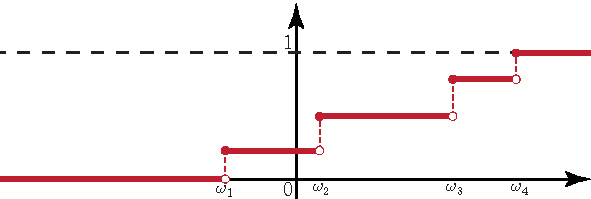
\includegraphics[width=0.4\paperwidth]{images/vadiscreta}
\end{center}
In particolare, $S$ è l'insieme delle discontinuità di $F_X$ e vale
\begin{equation}
	p_n=\lim_{x\to\omega_n^{+}}F_X(x)-\lim_{n\to\omega_n^{-}}F_X(x),\ \forall n\geq 1
\end{equation}
\subsection{Variabili aleatorie singolari continue}
\begin{define}[Variabili aleatorie singolari continue]
	$X$ si dice variabile aleatoria \textbf{singolare continua}\index{variabile aleatoria!singolare!continua} se $\mathbb{P}_X$ è \textbf{singolare continua} rispetto alla misura di Lebesgue $m_1$.\\
	Per definizione di misura singolare continua, esiste $S$ non numerabile con misura di Lebesgue nulla tale che,
	\begin{equation}
		\mathbb{P}_X\left(S\right)=1
	\end{equation}
\end{define}
\paragraph{Cdf di v.a. singolari continua}
La funzione di ripartizione $\funz{F_X}{\realset}{\left[0,1\right]}$ di una variabile aleatoria singolare continua è una funzione \textbf{continua} ma non \textit{assolutamente continua}.\\
In particolare, si dimostra che $F_X$ è derivabile su $\realset\setminus S$ (ossia \textbf{q.o.}) e
\begin{equation}
	F'_X(x)=0,\ \forall x\in\realset\setminus S
\end{equation}
\begin{observe}
	Questa condizione è compatibile con il fatto che $F_X$ sia crescente ed abbia come immagine $\left[0,1\right]$.
\end{observe}
\begin{examplewt}[Distribuzione di Cantor]
Una funzione ha la \textbf{distribuzione di Cantor}\index{distribuzione!di Cantor} se la sua funzione di ripartizione è la \textit{funzione di Cantor}\footnote{Si veda \refChapterOnly{teoriamisura}, teorema \ref{funzionecantor}, pag. \pageref{funzionecantor}.}.
\begin{center}
	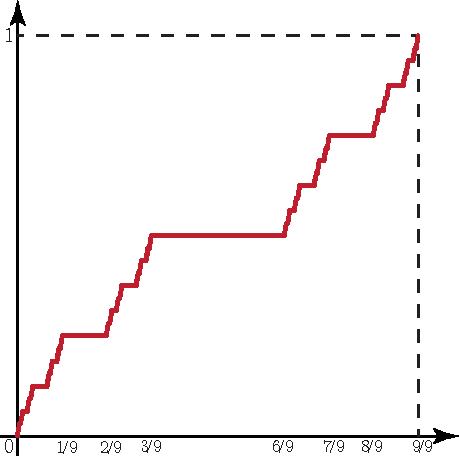
\includegraphics[width=0.4\paperwidth]{images/vasingolarecontinua}
\end{center}
Per quanto detto su tale funzione, essa soddisfa tutte le condizioni di essere la cdf di una variabile aleatoria singolarmente continua. In quanto tale, questa variabile aleatoria non ammette una funzione di densità, ma si può vedere, per simmetria.
\end{examplewt}
\subsection{Variabili aleatorie qualsiasi}
Abbiamo elencato tre diverse classi di misure di probabilità e variabili aleatorie ad esse associate. Il seguente teorema ci permette di affermare che esiste solo un'ulteriore classe di misure e variabili, le quali tuttavia non sono altro che combinazioni dei tre tipi precedentemente enunciati.
\begin{theoremaqed}[Teorema di Radon-Nikodym-Lebesgue]\index{teorema!di Radon-Nikodym-Lebesgue}
	Sia $\funz{\mathbb{P}}{\mathcal{B}\left(\realset\right)}{\left[0,1\right]}$ una misura di probabilità. Allora esistono $\alpha_1,\ \alpha_2,\ \alpha_3\geq 0$ e tre misure di probabilità $\mathbb{P}^{ac},\ \mathbb{P}^{sd},\ \mathbb{P}^{sc}$ assolutamente continua, singolare discreta e singolare continua, rispettivamente, tali che
	\begin{equation}
		\mathcal{P}=\alpha_1\mathbb{P}^{ac}+\alpha_2\mathbb{P}^{sd}+\alpha_3\mathbb{P}^{sc}\qedhere
	\end{equation}
\end{theoremaqed}
Come conseguenza, ogni variabile aleatoria si decompone nella somma di tre variabili aleatorie, una assolutamente continua, una discreta e una singolare continua.
\section{Modi di convergenza nella teoria della probabilità}
Come abbiamo potuto notare, la teoria assiomatica della probabilità è profondamente legata alla teoria della misura. Nella sezione \ref{modiconvergenza} abbiamo visto diversi modi in cui una successione di funzioni misurabili $\funz{f_n}{X}{\complexset}$ poteva convergere ad una funzione limite misurabile $\funz{f}{X}{\complexset}$. Studiamo ora i modi di convergenza di una successione di variabili aleatorie $\funz{X_n}{\Omega}{\complexset}$ ad una variabile aleatoria limite $\funz{X}{\Omega}{\complexset}$.
\paragraph{Convergenza puntuale o convergenza certa}
\begin{define}[Convergenza puntuale o convergenza certa]
	Consideriamo lo spazio di probabilità $\left(\Omega,\mathcal{F},\mathbb{P}\right)$ e le variabili aleatorie $\funz{X_n,X}{\Omega}{\complexset}$
	Si dice che $X_n$ \textbf{converge certamente}\index{convergenza!certa} a $X$\textbf{su} $\Omega$ ($X_n\overset{\text{c.}}{\to} X$) se
	\begin{equation}
		\lim_{n\to+\infty}X_n\left(\omega\right)=X\left(\omega\right),\ \forall \omega\in\Omega
	\end{equation}
\end{define}
La convergenza certa implica tutti i modi di convergenza successivi, ma \textit{non c'è alcun vantaggio} ad usare questa convergenza rispetto alla convergenza quasi certa.
\paragraph{Convergenza quasi certa}
\begin{define}[Convergenza quasi certa]
	Consideriamo lo spazio di probabilità $\left(\Omega,\mathcal{F},\mathbb{P}\right)$ e le variabili aleatorie $\funz{X_n,X}{\Omega}{\complexset}$
	Si dice che $X_n$ \textbf{converge quasi certamente}\index{convergenza!quasi certa} a $X$\textbf{su} $\Omega$ ($X_n\overset{\text{q.c.}}{\to} X$) se
	\begin{equation}
		\mathbb{P}\left(\left\{\omega\in\Omega \ \middle| \ \lim_{n\to+\infty}X_n\left(\omega\right)=X\left(\omega\right)\right\}\right)=1
	\end{equation}
\end{define}
Osserviamo che in uno spazio di probabilità $\left(\Omega,\mathcal{F},\mathbb{P}\right)$ questa convergenza è equivalente alla convergenza \textit{quasi ovunque}. Infatti:
\begin{align*}
	\left\{\omega\in \Omega\middle|\lim_{n\to+\infty}X_n\left(\omega\right)\neq X\left(\omega\right)\right\}&=\Omega\setminus\left\{\omega\in \Omega\middle|\lim_{n\to+\infty}X_n\left(\omega\right)= X\left(\omega\right)\right\}\\
	\mathbb{P}\left(\left\{\omega\in \Omega\middle|\lim_{n\to+\infty}X_n\left(\omega\right)\neq X\left(\omega\right)\right\}\right)&\underset{\mathbb{P}(x)<+\infty}{=}\mathbb{P}\left(\Omega\right)-\mathbb{P}\left(\left\{\omega\in \Omega\middle|\lim_{n\to+\infty}X_n\left(\omega\right)= X\left(\omega\right)\right\}\right)\\
	\mathbb{P}\left(\left\{\omega\in \Omega\middle|\lim_{n\to+\infty}X_n\left(\omega\right)\neq X\left(\omega\right)\right\}\right)&=1-\mathbb{P}\left(\left\{\omega\in \Omega\middle|\lim_{n\to+\infty}X_n\left(\omega\right)= X\left(\omega\right)\right\}\right)
\end{align*}
Allora affermare che
\begin{equation*}
	\mathbb{P}\left(\left\{\omega\in \Omega \ \middle| \ \lim_{n\to+\infty}X_n\left(\omega\right)= X\left(\omega\right)\right\}\right)=1
\end{equation*}
significa affermare che
\begin{equation*}
	\mathbb{P}\left(\left\{\omega\in \Omega \ \middle| \ \lim_{n\to+\infty}X_n\left(\omega\right)\neq X\left(\omega\right)\right\}\right)=0
\end{equation*}
\begin{attention}
	In uno spazio di misura che \textit{non} sia di probabilità questa corrispondenza non si può fare, dato che $\mu(X)$ può non essere pari ad $1$, tanto meno finito. Vale sempre la convergenza \textbf{q.o.}, ma mai quella \textbf{q.c.}.
\end{attention}
\newpage
\paragraph{Convergenza in probabilità}
\begin{define}[Convergenza in probabilità]
	Consideriamo lo spazio di probabilità $\left(\Omega,\mathcal{F},\mathbb{P}\right)$ e le variabili aleatorie $\funz{X_n,X}{\Omega}{\complexset}$. Si dice che	$X_n$ \textbf{converge in probabilità}\index{convergenza!in probabilità} a $X$ ($X_n\overset{\mathbb{P}}{\to} X$) se
	\begin{equation}
		\lim_{n\to+\infty}\mu\left(\left\{\omega\in \Omega\mid \abs{X_n\left(\omega\right)-X\left(\omega\right)}<\epsilon\right\}\right)=1,\ \forall \epsilon >0
	\end{equation}
\end{define}
In modo analogo alla convergenza quasi certa, in uno spazio di probabilità $\left(\Omega,\mathcal{F},\mathbb{P}\right)$ questa convergenza è equivalente alla \textit{convergenza in misura}.
\begin{attention}
	In uno spazio di misura che \textit{non} sia di probabilità questa corrispondenza non si può fare, dato che $\mu(X)$ può non essere pari ad $1$, tanto meno finito. Vale sempre la convergenza in misura, ma mai quella in probabilità.
\end{attention}
\paragraph{Convergenza in media}
\begin{define}[Convergenza in media]
	Consideriamo lo spazio di probabilità $\left(\Omega,\mathcal{F},\mathbb{P}\right)$ e le variabili aleatorie $\funz{X_n,X}{\Omega}{\complexset}$. Si dice che
	$X_n$ \textbf{converge in media}\index{convergenza!in media} a $f$ ($X_n\overset{L^1}{\to} X$) se
	\begin{equation}
		\lim_{n\to+\infty}\mathbb{E}X_n=\mathbb{E}X
	\end{equation}
	o, equivalentemente, se passiamo alla probabilità immagine,
	\begin{equation}
		\lim_{n\to+\infty}\int_\realset X_nd\mathbb{P}_Y=\int_{\realset}Xd\mathbb{P}_Y
	\end{equation}
\end{define}
\paragraph{Convergenza in legge}
\begin{define}[Convergenza in legge]
	Dato $\left(\Omega,\ \mathcal{M},\ \mathbb{P}\right)$ spazio di probabilità e le variabili aleatorie $\funz{X_n,\ X}{\Omega}{\realset}$ con le corrispettive \textit{funzioni di distribuzione}
	\begin{gather*}
		\funztot{F_n}{\realset}{\realset}{x}{F_n(x)=\mathbb{P}\left(X_n\leq x\right),\ \forall x\in \realset}\\
		\funztot{F}{\realset}{\realset}{x}{F(x)=\mathbb{P}\left(X\leq x\right),\ \forall x\in \realset}
	\end{gather*}
	allora si dice che $X_n$ converge a $X$ \textbf{in legge}\index{convergenza!in legge} $\left(X_n\stackrel{d}{\to}X\right)$ se
	\begin{equation}
		\lim_{n\to+\infty}F_n(x)=F(x),\ \forall x\in\realset\ \text{punto di continuità di }F.
	\end{equation}
\end{define}
%\part{Algebra Lineare}
%\labelPart{fourth}
%% SVN info for this file
\svnidlong
{$HeadURL$}
{$LastChangedDate$}
{$LastChangedRevision$}
{$LastChangedBy$}

\chapter{Approfondimenti di Algebra Lineare}
\labelChapter{jordan}

\begin{introduction}
	‘‘Non c'è quasi nessuna teoria più elementare dell'Algebra Lineare, nonostante il fatto che generazioni di professori e di scrittori di libri di testo ne abbiano oscurato la semplicità con calcoli assurdi con le matrici.''
	\begin{flushright}
		\textsc{Jean Dieudonné,} dopo aver visto quanto era lunga la dimostrazione della forma di Jordan.
	\end{flushright}
\end{introduction}
\lettrine[findent=1pt, nindent=0pt]{Q}{uesto} capitolo si può considerare un approfondimento di concetti ben noti dall'Algebra Lineare, cercando di rispondere alle seguenti questioni:
\begin{itemize}
	\item \textbf{\textsc{Diagonalizzazione simultanea}}: quando possiamo diagonalizzare due matrici con una \textit{stessa base} di autovettori?
	\item \textbf{\textsc{Polinomi e matrici}}: possiamo valutare un \textit{polinomio} con dei valori matriciali? Che relazione c'è fra polinomi matriciali e il \textit{polinomio caratteristico} della matrice?
	\item \textbf{\textsc{Forma canonica di Jordan}}: possiamo generalizzare la \textit{decomposizione spettrale} anche a matrici che non sono diagonalizzabili, rendendole così ‘‘più semplici''?
	\item \textbf{\textsc{Funzione esponenziale matriciale}}: come abbiamo fatto con i polinomi, possiamo ‘‘matricizzare'' la funzione esponenziale?
\end{itemize}
\section{Diagonalizzazione simultanea}
\begin{remember}
	Sia $V$ spazio vettoriale, su campo $\kamp$, di dimensione finita. Consideriamo gli \textbf{endomorfismi} di $V$ o, equivalentemente, le matrici $n\times n$ a elementi in $\kamp$ (con $\dim V=n$).
	\begin{itemize}
		\item $A$ determina un endomorfismo di $\kamp^n$ dato da $v\mapsto A\mathbf{v}$.
		\item Matrici associate allo stesso endomorfismo rispetto a basi diverse sono \textbf{simili}\index{matrice!simile}, cioè:
		\begin{equation}
			\exists P\in\gl\left(n\, \kamp\right)\ \colon B=P^{-1}AP
		\end{equation}
		\item Le seguenti affermazioni sono equivalenti:
		\begin{itemize}
			\item $A$ è \textbf{diagonalizzabile}\index{diagonalizzazione}.
			\item $A$ è simile ad una matrice diagonale $A=PDP^{-1}$ con $P$ matrice con \textbf{autovettori} sulle colonne.
			\item $\kamp^n$ ammette una base di \textbf{autovettori}\index{autovettore} di $A$.
			\item $\kamp^n=V_{\lambda_1}\oplus\ldots\oplus V_{\lambda_r}$ con $V_{\lambda_i}$ \textbf{autospazio}\index{autospazio} relativo ad $A$
		\end{itemize}
	\end{itemize}
\vspace{-3mm}
\end{remember}
\begin{define}[Diagonalizzazione simultanea.]~{}\\
	Siano $A,\ B\in\kamp^{n, m}$ due matrici \textit{diagonalizzabili}. Diciamo che $A$ e $B$ sono \textbf{simultaneamente diagonalizzabili}\index{diagonalizzazione!simultanea} se esiste una base di $\kamp^n$ composta di autovettori contemporaneamente sia di $A$ sia di $B$.\\
	Equivalentemente, $A$ e $B$ sono \textbf{simultaneamente diagonalizzabili} se esiste una matrice invertibile $P$ tale che $P^{-1}AP$ e $P^{-1}BP$ sono \textit{entrambe diagonali}.
\end{define}
\begin{example}
	Non tutte le matrici diagonalizzabili lo sono simultaneamente. Prendiamo $\realset^2$; si consideri:\\
	\begin{minipage}{.79\linewidth}
		\begin{itemize}
			\item $A$ diagonalizzabile con $2$ autovalori diversi, i cui autospazi sono le rette $y=x$ e $y=-x$.
		\end{itemize}
	\end{minipage}%\vspace{3mm}
	\begin{minipage}{.21\linewidth}\vspace{-5mm}
		\begin{equation*}
			A=\left(\begin{array}{cc}
				0 & 1 \\
				1 & 0
			\end{array}\right)
		\end{equation*}
	\end{minipage}	\\
	\begin{minipage}{.79\linewidth}
		\begin{itemize}
			\item $B$ diagonalizzabile con $2$ autovalori diversi, i cui autospazi sono le rette $y=0$ e $y=2x$.
		\end{itemize}
		\end{minipage}
	\begin{minipage}{.21\linewidth}\vspace{-4mm}
	\begin{equation*}
				B=\left(\begin{array}{cc}
					1 & -1 \\
					0 & -1
				\end{array}\right)
	\end{equation*}	
	\end{minipage}\\
Non esiste alcun autovettore comune, dunque $A$ e $B$ \textit{non} sono simultaneamente diagonalizzabili.
\end{example}
Dalla sola definizione non è semplice capire quali matrici sono a tutti gli effetti simultaneamente diagonalizzabili. Tuttavia, il seguente teorema ci permetterà di trovare una condizione necessaria e sufficiente per la diagonalizzazione simultanea.
\begin{theorema}[Diagonalizzazione simultanea se e solo se le matrici diagonalizzabili commutano.]~{}\label{teoremasimdiag}\\
Siano $A,\ B\in\kamp^{n, n}$. Allora $A$ e $B$ sono simultaneamente diagonalizzabili se e solo se $A$ e $ B$ sono diagonalizzabili e $A,\ B$ commutano, cioè $AB=BA$.
\end{theorema}
Per dimostrare il teorema, abbiamo tuttavia bisogno del seguente lemma:
\begin{lemming}[Matrici che commutano e autospazi.]~{}\\
	Siano $A,\ B\in\kamp^{n, n}$ tale che $AB=BA$ e sia $W$ un autospazio di $B$. Allora, presa l'azione di $\gl\left(n,\ \kamp\right)$ su $\kamp^{n, n}$, si ha che $A\ldotp W\subseteq W$.
\end{lemming}
\begin{demonstration}
	Sia $\lambda$ l'autovalore di $B$ relativo all'autospazio $W$. Per definizione di autospazio:
	\begin{equation*}
		W=\left\{\mathbf{v}\in V\mid B\ldotp \mathbf{v}=\lambda \mathbf{v}\right\}
	\end{equation*}
Sia $\mathbf{w}\in W$. Vogliamo mostrare che $A\ldotp \mathbf{w}\in W$.
\begin{equation*}
	B\ldotp\left(A\ldotp\mathbf{w}\right)=\left(BA\ldotp\mathbf{w}\right)=\left(AB\ldotp\mathbf{w}\right)=A\ldotp\left(B\ldotp\mathbf{w}\right)=A\ldotp\left(\lambda\mathbf{w}\right)=\lambda\left(A\ldotp\mathbf{w}\right)
\end{equation*}
$A\ldotp \mathbf{w}$ è autovettore rispetto a $\lambda$, pertanto $A\ldotp \mathbf{w}\in W,\ \forall \mathbf{w}$ e dunque segue la tesi.
\end{demonstration}
\begin{demonstration} \textsc{Dimostrazione del teorema} \ref{teoremasimdiag}.\\
	$\impliesdx$Per ipotesi, $\exists P\in \gl\left(n,\ \kamp\right)$ tale che $D_1=P^{-1}AP$ e $D_2=P^{-1}BP$ sono diagonali; in particolare, in quanto matrici diagonali, esse commutano: $D_1D_2=D_2D_1$. Allora $A=PD_1P^{-1}$ e $B=PD_2P^{-1}$.
	\begin{equation*}
		AB=\left(PD_1P^{-1}\right)\left(PD_2P^{-1}\right)=PD_1D_2P^{-1}=PD_2D_1P^{-1}=\left(PD_2P^{-1}\right)\left(PD_1P^{-1}\right)=BA
	\end{equation*}
$\impliessx$Procediamo con una \textit{dimostrazione costruttiva}. Sappiamo che:
\begin{itemize}
	\item $A$ diagonalizzabile $\implies \exists \mathbf{v}_1,\ \ldots,\ \mathbf{v}_n$ base di $V$ composta da \textit{autovettori} di $A$.
	\item $B$ diagonalizzabile $\implies V=W_1\oplus\ldots\oplus W_r$ con $W_j$ \textit{autospazi} di $B$
\end{itemize}
Consideriamo $\mathbf{v}_1\in V$. Esso si scrive in modo unico:
\begin{equation*}
	\textcolor{red}{\circled{{\ast}}}\quad \mathbf{v}_1=\mathbf{w}_{1,1}+\ldots+\mathbf{w}_{1,r}\text{ con }\mathbf{w}_{1,j}\in W_j,\ \forall j=1,\ \ldots,\ r
\end{equation*}
$\mathbf{v}_1$ è autovettore di $A$ relativo all'autovalore di $\lambda_1$, dunque $A\mathbf{v}_1=\lambda_1\mathbf{v}$. \textit{Moltiplichiamo} $\mathbf{v}_1$ per $A$:
\begin{equation*}
	\begin{array}{ccc}
		A\ldotp\mathbf{v}_1&=&A\ldotp\mathbf{w}_{1,1}+\ldots+A\ldotp\mathbf{w}_{1,r}\\
		\shortparallel&\\
		\lambda_1\mathbf{v}_1&=&\lambda_1\mathbf{w}_{1,1}+\ldots+\lambda_1\mathbf{w}_{1,r}
	\end{array}
\end{equation*}
Dal lemma appena dimostrato, da $A\ldotp W_j\subseteq W_j,\ \forall j$ segue che $A\ldotp \mathbf{w}_j\in W_j$. Per la chiusura di $W_j$ rispetto al prodotto per uno scalare, abbiamo anche $\lambda \mathbf{w}_j\in W_j,\ \forall j$. Siccome in una somma diretta la decomposizione è unica, deduciamo che:
\begin{equation*}
	A\ldotp \mathbf{w}_{1,1}=\lambda_1 \mathbf{w}_{1,1},\ \ldots,\ A\ldotp \mathbf{w}_{1,r}=\lambda_1 \mathbf{w}_{1,r}
\end{equation*}
In altre parole, $\forall j,\ \mathbf{w}_{1,j}$ è $\mathbf{0}$ oppure un autovettore di $A$ e, per ipotesi, anche di $B$. Procediamo allo stesso modo tutti i vettori della base $\mathbf{v}_1, \ldots,\ \mathbf{v}_n$: si ha che $\mathbf{v}_i=\mathbf{w}_{i,1}+\ldots+\mathbf{w}_{i,r}$ e $\forall i, j,\ $ $\mathbf{w}_{i,j}$ è $\mathbf{0}$ oppure un autovettore comune di $A$ e $B$.\\
Otteniamo un insieme $\left\{\mathbf{w}_{i, j}\right\}$ di autovettori comuni di $A$ e $B$. Per costruzione, lo \textit{span lineare} dei $\left\{\mathbf{w}_{i, j}\right\}$ contiene $\left\{\mathbf{v}_1,\ \ldots,\ \mathbf{v}_n\right\}$ e pertanto è necessariamente pari a $V$!\\
In altre parole, $\left\{\mathbf{w}_{i,\ j}\right\}$ è un sistema di generatori di $V$ e possiamo estrarre da esso una base di $V$ costituita di autovettori comuni ad $A$ e a $B$.
\end{demonstration}
\section{Polinomi e matrici}
\begin{remember}
	Dato un campo $\kamp$, indichiamo con $\kamp\left[t\right]$ l'anello dei polinomi a coefficienti in $\kamp$ nella variabile $t$; un suo elemento $f\left(t\right)\in\kamp\left[t\right]$ è della forma:
	\begin{equation}
		f\left(t\right)=b_nt^n+b_{n-1}t^{n-1}+\ldots+b_1t+b_0\text{ con }b_i\in\kamp
	\end{equation}
\vspace{-6mm}
\end{remember}
Finora abbiamo sempre \textit{valutato} i polinomi in valori del campo $\kamp$. Possiamo invece valutarli in una \textit{matrice} in $\kamp^{n, n}$? Dopotutto, la \textit{somma di matrici} e la \textit{moltiplicazione per uno scalare} sono operazioni \textit{interne} a $\kamp^{n, n}$ e pertanto potremmo pensare che sia lecito.\\
Tuttavia, presi i polinomi $p$ così come sono, non sarebbe \textit{ben definita} $p\left(A\right)$ a causa del \textbf{termine noto}; infatti, non possiamo sommare uno \textit{scalare ad una matrice}! Per ovviare a questo problema, quando valutiamo un polinomio in una matrice $A$ ‘‘\textit{correggiamo}'' il termine noto con la \textbf{matrice identità} $I$:
\begin{equation}
	f\left(A\right)\coloneqq b_nA^n+b_{n-1}A^{n-1}+\ldots+b_1A+b_0I\text{ con }b_i\in\kamp
\end{equation}
In questo modo, $f\left(A\right)\in\kamp^{n, n}$.
\begin{example}
Preso $f\left(t\right)=t^2-3$, il polinomio valutato nella matrice $A$ è $f\left(A\right)=A^2-3I$.
\end{example}
\begin{observe}
	Dati $f,\ g\in\kamp\left[t\right]$ e $A\in\kamp^{n,n}$, si ha:
	\begin{itemize}
		\item $\left(f+g\right)\left(A\right)=f\left(A\right)+g\left(A\right)$.
		\item $\left(fg\right)\left(A\right)=f\left(A\right)g\left(A\right)$
	\end{itemize}
\vspace{-3mm}
\end{observe}
\begin{demonstration}
	Prendiamo i polinomi $f\left(t\right)=b_nt^n+b_{n-1}t^{n-1}+\ldots+b_1t+b_0$ e $g\left(t\right)=c_nt^n+c_{n-1}t^{n-1}+\ldots+c_1t+c_0$ e valutiamoli entrambi in $A$: $f\left(A\right)=b_nA^n+b_{n-1}A^{n-1}+\ldots+b_1A+b_0I$ e $g\left(A\right)=c_nA^n+c_{n-1}A^{n-1}+\ldots+c_1A+c_0I$.
	\begin{enumerate}[label=\Roman*]
		\item La somma è ovvia.
		\item Il prodotto è garantito dalla commutatività delle potenze di matrici.
	\end{enumerate}
\vspace{-3mm}
\end{demonstration}
\subsection{Ideale di una matrice}
\begin{define}[Ideale di una matrice.]~{}\\
	Data $A\in\kamp^{n,n}$, definiamo l'\textbf{ideale della matrice}\index{ideale!di una matrice}:
	\begin{equation}
		I_A\coloneqq\left\{f\in\kamp\left[t\right]\mid f\left(A\right)=O\right\}
	\end{equation}
\vspace{-6mm}
\end{define}
\begin{observe}~{}
	\begin{itemize}
		\item $0\in I_A$.
		\item $I_A\neq\left\{0\right\}$; infatti, se consideriamo le seguenti $n^2+1$ matrici in $\kamp^{n,n}$:
		\begin{equation*}
			I,\ A,\ A^2,\ A^3,\ \ldots,\ A^{n^2}
		\end{equation*}
	Per il lemma di Steinitz queste matrici sono necessariamente \textit{linearmente dipendenti}, dato che superano in numero $\dim \kamp^{n,n}=n^2$, cioè esistono i coefficienti $a_0,\ \ldots,\ a_{n^2}\in\kamp$ \textit{non} tutti nulli tali che:
	\begin{equation*}
		a_0I+a_1A+a_2A^2+\ldots+a_{n^2}A^{n^2}=O
	\end{equation*}
	Allora $p\left(t\right)=a_{n^2}t^{n^2}+\ldots+a_2t^2+a_1t+a_0$ è un polinomio \textit{non} nullo in $I_A$.
	\item $I_A$ soddisfa giustamente la definizione di \textbf{ideale}\index{ideale} di $\kamp\left[t\right]$:
	\begin{itemize}
		\item \textsc{$I_A$ è un sottogruppo di $\left(\kamp^{n, n},\ +\right)$}.
		\begin{equation*}
			\left(f+g\right)\left(A\right)=f\left(A\right)+g\left(A\right)=0\implies f+g\in I_A
		\end{equation*}
		\item \textsc{Assorbimento}: se $h\in\kamp\left[t\right]$ si ha :
		\begin{equation*}
			\left(fh\right)\left(A\right)=\underbrace{f\left(A\right)}_{=O}h\left(A\right)=O\implies fh\in I_A
		\end{equation*}
	\end{itemize}
	\end{itemize}
\vspace{-3mm}
\end{observe}
\subsection{Polinomio minimo}
\begin{proposition}[Anello ${\kamp\left[t\right]}$ è ad ideali principali.]~{}\\
	L'anello $\kamp\left[t\right]$ è ad \textit{ideali principali}: se $I\subseteq \kamp\left[t\right]$ è un ideale, $\exists p$ tale che $I=\left(p\right)$. Il generatore $p$ è \textit{unico} a meno di moltiplicazione per scalari \textit{non} nulli, se prendiamo $p$ \textbf{monico} allora è unico.
\end{proposition}
\begin{demonstration}
Sia $p\in I$ un polinomio \textit{non} nullo di grado \textit{minimo} tra i polinomi in $I_A$.\\
Se $p$ è \textit{costante}, allora $I=\kamp\left[t\right]=\left(1\right)=\left(p\right)$.\\
Supponiamo allora $p$ \textit{non} costante. Vogliamo mostrare che $p$ genera $I$.
Prendiamo $f\in I$ e dividiamolo per $p$:
\begin{equation*}
	\underbrace{f\left(t\right)}_{\in I}=\underbrace{p\left(t\right)q\left(t\right)}_{\in I\text{ per assorbimento}}+r\left(t\right)
\end{equation*}
Con $r\left(t\right)$ polinomio con $\deg r < \deg p$. Notiamo che anche $r\left(t\right)\in I$ per essere vera l'equazione di sopra; in particolare, per la minimalità del grado di $p$ non può esserci un polinomio in $I$ di grado minore di $p$, dunque $r\equiv 0$. Allora $p\mid f$ e dunque ogni polinomio in $I$ è generato da $p$: $I\equiv\left(p\right)$.\\
Se $I=\left(p\right)=\left(\widetilde{p}\right)$, allora $p,\ \widetilde{p}\in I$ e dunque $p\mid \widetilde{p}$, $\widetilde{p}\mid p$, cioè $p=\lambda\widetilde{p}$ con $\lambda\in\kamp\setminus\left\{0\right\}$. Se $p$ è \textit{monico}, l'unico coefficiente $\lambda$ per cui si ha $p=\lambda\widetilde{p}$ è $1$, e dunque $p=\widetilde{p}$, cioè $p$ è unico.
\end{demonstration}
\begin{define}[Polinomio minimo.]~{}\\
	Sia $A\in\kamp^{n, n}$ e sia $I_A$ ideale dei polinomi che si annullano in $A$. Il \textbf{polinomio minimo}\index{polinomio!minimo} $m_A\left(t\right)$ di $A$ è il  \textit{generatore monico} di $I_A$, ovvero è il polinomio monico \textit{non} nullo di grado minimo tra i polinomi in $I_A$.
\end{define}
\begin{example} Cerchiamo il polinomio minimo della seguente matrice.
	\begin{equation*}
		A=\left(\begin{array}{cc}
			0 & 1 \\
			1 & 0
		\end{array}\right)\quad A^2=\left(\begin{array}{cc}
		0 & 1 \\
		1 & 0
	\end{array}\right)\left(\begin{array}{cc}
	0 & 1 \\
	1 & 0
\end{array}\right)=\left(\begin{array}{cc}
1 & 0 \\
0 & 1
\end{array}\right)=I
	\end{equation*}
Notiamo che $A^2-I=O$, dunque $p\left(t\right)=t^2-1\in I_A$. Poiché $m_A\left(t\right)\mid p\left(t\right)$, esso può essere solo $t-1$, $t+1$, $t^2-1$. Escludiamo sempre il caso $m_A\left(t\right)=1$, in quanto allora si avrebbe $I_A=\kamp\left[t\right]$ e ciò non è mai vero per questo anello (i polinomi di grado $0$ non si annullano in generale sulle matrici!).\\
Se fosse $m_A\left(t\right)=t-1$, allora $m_A\left(A\right)=A-I\neq O$ e dunque $t-1\notin I_A$. In modo analogo $m_A\left(t\right)=t+1\implies A+I\neq 0\implies t-1\notin I_A$. L'unica possibilità è allora $m_A\left(t\right)=t^2-1$.
\end{example}
\begin{observe}
	Se $A$ e $B$ sono simili, allora $I_A=I_B\subseteq \kamp\left[t\right]$ e quindi $m_A\left(t\right)=m_B\left(t\right)$.
\end{observe}
\begin{demonstration}
	Sia $M\in\gl\left(n,\ \kamp\right)$ la matrice che rende $A$ simile a $B$: $B=M^{-1}AM$. Le potenze di matrici simili sono simili anch'esse:
	\begin{equation*}
		\begin{array}{l}
			B=M^{-1}AM\\
			B^2=M^{-1}A^2M\\
			\ldots\\
			B^k=M^{-1}A^kM
		\end{array}
	\end{equation*}
Se $p\left(t\right)=c_dt^d+\ldots+c_0$, allora:
\begin{equation*}
	\begin{array}{ll}
		M^{-1}p\left(A\right)M&=M^{-1}\left(c_dA^d+\ldots+c_0I\right)M=c_d\left(M^{-1}A^dM\right)+\ldots+c_1\left(M^{-1}AM\right)+c_0I=\\
		&=c_dB^d+\ldots+c_1B+c_0I=p\left(B\right)
	\end{array}
\end{equation*}
Ovvero $M^{-1}p\left(A\right)M=\left(B\right)$. Pertanto, $p\left(A\right)=O$ se e solo se $p\left(B\right)=O$, cioè se $I_A=I_B$.
\end{demonstration}
\section{Teorema di Cayley-Hamilton}
\begin{remember}
	Ricordiamo alcune definizioni e proprietà utili legate al \textbf{determinante}:
	\begin{itemize}
		\item Il \textbf{complemento algebrico}\index{completamento algebrico} $\left(i,\ j\right)$ di una matrice quadrata $M$ è:
		\begin{equation}
			M_{i,j}=\left(-1\right)^{i+j}\det\left(\begin{array}{c}
				\text{matrice ottenuta da }M \text{ cancellando}\\
				\text{la riga }i\text{ e la colonna }j
			\end{array}\right)
		\end{equation}
	\item La \textbf{matrice aggiunta}\index{matrice!aggiunta} $\mathrm{adj}\left(M\right)$ di una matrice quadrata $M$ è la matrice $\left(M_{i,j}\right)$ che, al posto $\left(i,\ j\right)$ ha il complemento algebrico $M_{j,i}$.\footnote{Attenzione all'ordine degli indici!}
	\item La \textbf{regola di Laplace}\index{regola!di Laplace} afferma che:
	\begin{equation}
		\mathrm{adj}\left(M\right)M=M\mathrm{adj}\left(M\right)=\det\left(M\right)I
	\end{equation}
	Inoltre, se $\det\left(M\right)\neq 0$, allora:
	\begin{equation}
		M^{-1}=\frac{1}{\det M}\mathrm{adj}\left(M\right)
	\end{equation}
\item Il \textbf{polinomio caratteristico}\index{polinomio!caratteristico} di $A$ è:
\begin{equation}
	C_A\left(t\right)=\det\left(tI-A\right)=\left(-1\right)^n\det\left(A-tI\right)
\end{equation}
In particolare, il polinomio caratteristico è un polinomio \textit{monico}.
	\end{itemize}
\vspace{-3mm}
\end{remember}
\begin{observe}\label{polinomicoeffmatrisci}
Una matrice i cui elementi sono polinomi in $\kamp\left[t\right]$ può essere scritta in modo unico come polinomio in $t$ con coefficienti delle matrici in $\kamp^{n,n}$.
\end{observe}
\begin{example}~{}
	\begin{equation*}
		\left(\begin{array}{cc}
			2t^2 & 3t+1 \\
			t^2-4t & 0
		\end{array}\right)=\left(\begin{array}{cc}
		2 & 0 \\
		1 & 0
	\end{array}\right)t^2+\left(\begin{array}{cc}
	0 & 3 \\
	-4 & 0
\end{array}\right)t+\left(\begin{array}{cc}
0 & 1 \\
0 & 0
\end{array}\right)
	\end{equation*}
\end{example}
\begin{theorema}[Teorema di Cayley-Hamilton.]~{}\index{teorema!di Cayley-Hamilton}\\
Sia $A\in \mathbb{K}^{n,n}$. Allora $C_A\left(t\right)\in I_A$, cioè $C_A\left(A\right)=0$. In altre parole, $m_A\left(t\right)\mid C_A\left(t\right)$.\\
In particolare $\deg m_A\left(t\right)\leq n$.
\end{theorema}
\begin{demonstration}
	Sia $M\coloneqq tI-A$. Allora:
	\begin{equation*}
		C_A\left(t\right)=\det M=t^n+b_{n-1}t^{n-1}+\ldots+b_1t+b_0
	\end{equation*}
Consideriamo l'\textit{aggiunta} di $M$, $\mathrm{adj}\left(M\right)=\mathrm{adj}\left(tI-A\right)$.
Poiché gli elementi di $tI-A$ sono polinomi in $\kamp\left[t\right]$ di grado minore o uguale di $1$ e gli elementi di $\mathrm{adj}\left(M\right)$ sono polinomi in $\kamp\left[t\right]$ di grado minore o uguale di $n-1$, $\mathrm{adj}\left(M\right)$ si scrive come polinomio di grado minore e uguale a $n-1$ con coefficienti in $\kamp^{n, n}$ (grazie all'osservazione di pag. \pageref{polinomicoeffmatrisci}).
\begin{equation*}
	\mathrm{adj}\left(M\right)=C_{n-1}t^{n-1}+C_{n-2}t^{n-2}+\ldots+C_1t+C_0,\ C_i\in\kamp^{n,n}
\end{equation*}
Usando la regola di Laplace:
\begin{equation*}
	\begin{array}{ccc}
		M\mathrm{adj}\left(M\right)=\det\left(M\right)I&&\\
		\Downarrow&&\\
		\left(tI-A\right)\mathrm{adj}\left(M\right)=C_A\left(t\right)I&=&\left(t^n+b_{n-1}t^{n-1}+\ldots+b_1t+b_0\right)I\\
		\shortparallel &=& \ovaled{It^n+b_{n-1}It^{n-1}+\ldots+b_1It+b_0I}\\
		\left(tI-A\right)\left(C_{n-1}t^{n-1}+C_{n-2}t^{n-2}+\ldots+C_1t+C_0\right)&&\\
		={\tikz[baseline=(char.base)]\node[anchor=south west, draw,rectangle, rounded corners, inner sep=2pt, minimum size=7mm,
		text height=6mm](char){$\begin{array}{l}
				{\small C_{n-1}t^n+C_{n-2}t^{n-1}+\ldots+C_1t^2+C_0t+}\\
				{\small-AC_{n-1}t^{n-1}-AC_{n-2}t^{n-2}+\ldots-AC_1t+AC_0}
			\end{array}$} ;}&&
	\end{array}
\end{equation*}
Uguagliamo i due termini evidenziati, sommando le matrici coefficienti termine a termine. Si ha il sistema:
\begin{equation*}
	\begin{cases}
		\begin{array}{ll}
			C_{n-1}=I&\colon t^n\\
			C_{n-2}-AC_{n-1}=b_{n-1}I&\colon t^{n-1}\\
			C_{n-3}-AC_{n-2}=b_{n-2}I&\colon t^{n-2}\\
			\ldots&\\
			C_{0}-AC_{1}=b_{1}I&\colon t\\
			-AC_0=b_0I&\colon 1\\
		\end{array}
	\end{cases}
\end{equation*}
Sostituiamo a cascata le equazioni dalla seconda in giù:
\begin{equation*}
	\begin{cases}
		\begin{array}{ll}
			C_{n-2}=A+b_{n-1}I\\
			C_{n-3}=A^2+b_{n-1}A+b_{n-2}I\\
			\ldots\\
			C_0=A^{n-1}+b_{n-1}A^{n-2}+\ldots+b_1I
		\end{array}
	\end{cases}
\end{equation*}
Sostituiamo $C_0$ nell'ultima:
\begin{equation*}
	\underbrace{A^n+b_{n-1}A^{n-1}+\ldots+b_1A+b_0I}_{C_A\left(A\right)}=O
\end{equation*}
Abbiamo dunque ottenuto la tesi.
\end{demonstration}
\begin{observe}
	Si ha che $m_A\left(t\right)\mid C_A\left(t\right)\implies C_A\left(t\right)=m_A\left(t\right)q\left(t\right)$, con $q\left(t\right)\in\kamp\left[t\right]$. In altre parole, le \textit{radici} del \textit{polinomio minimo} sono \textit{autovalori}.
\end{observe}
Il seguente teorema afferma un legame ancora più forte tra polinomio minimo e autovalori di una matrice.
\begin{theorema}[Radici del polinomio minimo sono autovalori di $A$ e viceversa.]~{}\\
	Sia $A\in \kamp^{n,n}$ e $m_A\left(t\right)$ il suo polinomio minimo. Allora, preso $\lambda\in\kamp$:
	\begin{equation}
		m_A\left(\lambda\right)=0\iff \lambda\text{ è un autovalore di }A
	\end{equation}
\vspace{-6mm}
\end{theorema}
\begin{demonstration}~{}\\
	$\impliesdx$Segue dal teorema di Cayley-Hamilton perché $m_A\left(\lambda\right)=0\implies C_A\left(\lambda\right)=0\implies \lambda$ autovalore.\\
	$\impliessx$Sia $\lambda$ un autovalore di $A$ con autovettore associato $\mathbf{v}$. Si ha:
	\begin{gather*}
		A\mathbf{v}=\lambda \mathbf{v}\\
		A^2\mathbf{v}=A\left(A\mathbf{v}\right)=A\left(\lambda \mathbf{v}\right)=\lambda A\mathbf{v}=\lambda^2 \mathbf{v}\\
	\end{gather*}
Allo stesso modo si arriva a $A^k\mathbf{v}=\lambda^k\mathbf{v}$. Preso un generico polinomio $p\left(t\right)\in\kamp\left[t\right]$, esso si può esprimere come:
\begin{equation*}
	p\left(t\right)=\sum_{i=0}^{d}c_i t^i\quad c_i\in\kamp
\end{equation*}
Allora $\displaystyle p\left(A\right)=\sum_{i=0}^{d}c_i A^i$ e dunque:
\begin{align*}
	p\left(A\right)\mathbf{v}&=\left(\sum_{i=0}^{d}c_i A^i\right)\mathbf{v}=\sum_{i=0}^{d}c_i\left( A^i\mathbf{v}\right)=\sum_{i=0}^{d}c_i\left( \lambda^i\mathbf{v}\right)=\underbrace{\left(\sum_{i=0}^{d}c_i \lambda^i\right)}_{\in\kamp}\mathbf{v}=p\left(\lambda\right)\mathbf{v}
\end{align*}
Consideriamo ora un polinomio $p\in I_A$. Per sua definizione $p\left(A\right)=0$; in particolare, da quanto scritto sopra:
\begin{equation*}
	O\mathbf{v}=p\left(\lambda\right)\mathbf{v}
\end{equation*}
Ed essendo $v$ un autovettore, $v\neq 0$; dall'equazione sopra necessariamente segue $p\left(\lambda\right)=0$. In particolare, essendo $p\in I_A$ generato dal polinomio minimo $m_A$ (cioè $p\left(t\right)=m_A\left(t\right)q\left(t\right)$ con $q\left(t\right)\neq 0$), segue che $m_A\left(\lambda\right)=0$.
\end{demonstration}
\section{Forma canonica di Jordan}
D'ora in poi, se non altresì specificato, considereremo $\kamp=\complexset$, cioè tratteremo di matrici $A\in \complexset^{n,n}$ e endomorfismi fra spazi vettoriali complessi.
\begin{observe}\label{complessichiusi}
Poiché $\complexset$ è \textbf{algebricamente chiuso}, ogni polinomio $p\in\complexset\left[t\right]$ si fattorizza completamente come prodotto di fattori lineari:
\begin{equation}
	C_A\left(t\right)=\left(t-\lambda_1\right)^{m_1}\ldots\left(t-\lambda_r\right)^{m_r}\text{ con } m_i \text{ molteplicità algebrica di } \lambda_i
\end{equation}
Nel caso del polinomio minimo, si ha:
\begin{equation}
	m_A\left(t\right)=\left(t-\lambda_1\right)^{h_1}\ldots\left(t-\lambda_r\right)^{h_r}\text{ con } 1\leq h_i\leq m_i\ \forall i=1,\ldots,\ r
\end{equation}
Come altra conseguenza, ogni matrice $n\times n$ ammette $n$ autovalori complessi, contati con la loro molteplicità.
\end{observe}
Sia $A\in \complexset^{n,n}$ una matrice associata a un endomorfismo $\funz{f}{V}{V}$. Se $f$ è diagonalizzabile, esiste una base in cui la matrice di $f$ è diagonale. Anche quando tuttavia la matrice non è diagonalizzabile, vogliamo cercare una base in cui la matrice di $f$ è \textit{particolarmente semplice}.
\begin{define}[Blocco di Jordan.]~{}\\
	Un \textbf{blocco di Jordan}\index{blocco di Jordan} $J=J_k\left(\lambda\right)$, di autovalore $\lambda\in\complexset$ e dimensione $k$, è una matrice quadrata $k\times k$ con sulla diagonale solo l'autovalore e sopra ogni elemento della diagonale $1$:
	\begin{equation}
		    J=J_k\left(\lambda\right) = \left(
		\begin{array}{ccccc}
\lambda	& 1 		&  0		& \ldots 	& 0 \\
0		& \lambda 	& \ddots	& 			& \vdots\\
\vdots	&  			& \ddots	& 1 		& 0\\
\vdots	& 			&   		& \lambda 	& 1\\
0		&  \dots  	&  \dots 	&  0 		& \lambda
		\end{array}
		\right)
	\end{equation}
\end{define}
\begin{observes}~{}
	\begin{itemize}
		\item $J$ è determinato da $\lambda$ e $k$.
		\item Il polinomio caratteristico di $J$ è $C_J\left(t\right)=\left(t-\lambda\right)^k$, cioè $\lambda$ è l'unico autovalore di $J$ con molteplicità algebrica $k$.
	\end{itemize}
\vspace{-3mm}
\end{observes}
\begin{observe}\label{bloccojordanbase}
Definiamo il blocco di Jordan di dimensione $k$ con autovalore zero, necessario per calcolare l'autospazio $V_\lambda$:
		\begin{equation}\setlength\arraycolsep{0.5mm}
			N=J-\lambda I= \left(
				\begin{array}{ccccc}
				0	& 1 		&  0		& \ldots 	& 0 \\
				0		& 0 	& \ddots	& 			& \vdots\\
				\vdots	&  			& \ddots	& 1 		& 0\\
				\vdots	& 			&   		& 0 	& 1\\
				0		&  \dots  	&  \dots 	&  0 		& 0
			\end{array}
			\right)
		\end{equation}
Si ha che $\rk N=k-1\implies \dim V_{\lambda}=\dim \ker N=k-\rk N= 1$, cioè $J$ \textit{non} è \textit{mai} diagonalizzabile se $k>1$, dato che $1=\dim V_{\lambda}\leq m_\lambda = k$.\\
Se la base $\basis$ dello spazio $V$ (in cui stiamo operando con l'endomorfismo associato a $J$) è $\left\{\mathbf{e}_1,\ \ldots,\ \mathbf{e}_k\right\}$, notiamo che $\mathbf{e}_1$ è l'unico autovettore di $N$ e $V_\lambda=\mathcal{L}\left(\mathbf{e}_1\right)$. Si vede che $J$ agisce in modo particolare sui vettori di $\basis$:
\begin{equation*}
\begin{cases}
J\mathbf{e}_1=\lambda \mathbf{e}_1\\
J\mathbf{e}_2=\mathbf{e}_1+\lambda \mathbf{e}_2\\
\ldots\\
J\mathbf{e}_k=\mathbf{e}_{k-1}+\lambda \mathbf{e}_k
\end{cases}
\end{equation*}
Anche $N$ agisce in modo altrettanto particolare sui vettori di $\basis$:
\begin{equation*}
	\begin{cases}
		N\mathbf{e}_1=\mathbf{0}\\
		N\mathbf{e}_2=\mathbf{e}_1\\
		\ldots\\
		N\mathbf{e}_k=\mathbf{e}_{k-1}
	\end{cases}
\end{equation*}
Cioè, cominciando da $\mathbf{e}_k$ e applicando $N$ ripetutamente otteniamo gli altri vettori della base.
\begin{center}
	\begin{tikzcd}
		\mathbf{e}_{1} & \mathbf{e}_{2} \arrow[l, "N", bend left] & \dots \arrow[l, "N", bend left] & \mathbf{e}_{k-1} \arrow[l, "N", bend left] & \mathbf{e}_k \arrow[l, "N", bend left]
	\end{tikzcd}
\end{center}
Ad esempio, con $N^2$ si ha:
\begin{equation*}
	\begin{cases}
		N^2\mathbf{e}_1=\mathbf{0}\\
		N^2\mathbf{e}_2=N\left(N\mathbf{e}_2\right)=N\mathbf{e}_1=\mathbf{0}\\
		\ldots\\
		N^2\mathbf{e}_k=N\left(N\mathbf{e}_k\right)=N\mathbf{e}_{k-1}=\mathbf{e}_{k-2}
	\end{cases}
\end{equation*}
Infatti, se guardiamo la matrice $N^2$, si ha:
		\begin{equation*}
	N^2=\left(J-\lambda I\right)^2= \left(
	\begin{array}{ccccc}
		0		& 0 		&  1		& \ldots 	& 0 \\
		\vdots	& \ddots 	& 0			& 1			& \vdots\\
				&  			& \ddots	& 0 		& 1\\
		\vdots	& 			&   		& \ddots 		& 0\\
		0		&  \dots  	&  \dots 	& \dots 		& 0
	\end{array}
	\right)
\end{equation*}
Si ha dunque, ad ogni potenza successiva di $N$, lo ‘‘spostamento'' della diagonale di $1$ verso destra. In particolare:
		\begin{equation*}
	N^{k-1}=\left(J-\lambda I\right)^{k-1}= \left(
	\begin{array}{ccccc}
		0		& \dots 	&  	\dots		& 0 	& 1 \\
		\vdots	& \ddots 	& 			& 		& 0\\
				&  			& 			&  		& \vdots \\
		\vdots	& 			&   		& \ddots 		& \vdots\\
		0		&  \dots  	&  \dots 	& \dots & 0
	\end{array}
	\right)
\end{equation*}
E in questo caso si ha la relazione con i vettori della base:
\begin{equation*}
	\begin{cases}
		N^{k-1}\mathbf{e}_i=\mathbf{0}\ \forall i=1,\ldots,\ k-1\\
		\ldots\\
		N^{k-1}\mathbf{e}_k=\mathbf{e}_1
	\end{cases}
\end{equation*}
Studiando l'immagine dell'applicazione associata ad $N$, poiché la base dell'immagine sono i vettori colonna linearmente indipendenti, si ha $\im N^{k-1}=\mathcal{L}\left(e_1\right)$.\\
Come già affermato dunque, è $\mathbf{e}_k$ a determinare l'\textit{intera} base di $V$ tramite la moltiplicazione per $N$.\\
Come ultima osservazione fondamentale, notiamo inoltre che $N^k=O$, cioè $N$ è una matrice \textbf{nilpotente}\index{matrice!nilpotente} di ordine $k$.
\end{observe}
\begin{define}[Forma di Jordan.]~{}\\
	Una matrice quadrata si dice in \textbf{forma di Jordan}\index{forma di Jordan} se ha \textit{solo} blocchi di Jordan lungo la diagonale, mentre altrove è nulla.
\end{define}
\begin{example}
La seguente matrice $9\times 9$ è in forma di Jordan con $J_3\left(2\right)$, $J_2\left(i\right)$, $J_3\left(i\right)$ e $J_1\left(-4\right)$:
	\begin{equation*}
		A=
		\tikz[baseline]{
			\node[matrix of math nodes,matrix anchor=west,left delimiter=(,right delimiter=),ampersand replacement=\&] (M) {
				2 	\& 1 	\& 0	\& \color{gray}{0}	\&	\color{gray}{0} 	\&	\color{gray}{0} 	\&	\color{gray}{0} 	\&	\color{gray}{0} 	\&	\color{gray}{0} 	\\
				0	\& 2 	\& 1 	\& \color{gray}{0}	\&	\color{gray}{0}	\&	 \color{gray}{0}	\&	\color{gray}{0} 	\&	\color{gray}{0} 	\&	\color{gray}{0} 	\\
				0	\& 0 	\& 2 	\& \color{gray}{0}	\& \color{gray}{0}	\&	\color{gray}{0}	\&	\color{gray}{0} 	\&	\color{gray}{0} 	\&	\color{gray}{0} 	\\
				\color{gray}{0}	\& \color{gray}{0} 	\& \color{gray}{0}  	\& i	\& 1	\&	\color{gray}{0}	\&	\color{gray}{0} 	\&	\color{gray}{0} 	\&	\color{gray}{0} 	\\
				\color{gray}{0}	\& \color{gray}{0} 	\& \color{gray}{0} 	\& 0	\& i	\&	\color{gray}{0}	\&	\color{gray}{0}	\&	\color{gray}{0}	\&	\color{gray}{0}	\\
				\color{gray}{0}	\&  \color{gray}{0}	\& \color{gray}{0} 	\& \color{gray}{0}	\& \color{gray}{0}	\&	i	\&	1	\&	0	\&	\color{gray}{0}	\\
				\color{gray}{0}	\& \color{gray}{0} 	\& \color{gray}{0}  	\& 	\color{gray}{0}	\& \color{gray}{0}	\&	0	\&	i	\&	1 	\&	\color{gray}{0}	\\
				\color{gray}{0}	\&  \color{gray}{0}	\&  \color{gray}{0} 	\& \color{gray}{0}		\& \color{gray}{0}	\&	0	\&	0	\&	i 	\&	\color{gray}{0}	\\
				\color{gray}{0}	\& \color{gray}{0} 	\&  \color{gray}{0} 	\& \color{gray}{0}		\& \color{gray}{0}	\&	\color{gray}{0}	\&	\color{gray}{0}	\&	\color{gray}{0} 	\&	-4	\\				
			};
			\draw (M-1-1.north west) rectangle (M-3-3.south east);
			\draw (M-3-3.south east) rectangle (M-5-5.south east);
			\draw (M-5-5.south east) rectangle (M-8-8.south east);
			\draw (M-8-8.south east) rectangle (M-9-9.south east);
		}
	\end{equation*}
\end{example}

\begin{observe}
	Una matrice \textit{diagonale} è in forma di Jordan, con \textbf{solo} blocchi di ordine $1$ (cioè senza alcun $1$ sopra la diagonale).
\end{observe}
\begin{observe}\label{molteplicitàalgebrichedijordan}
	Se $A$ è in forma di Jordan, sulla diagonale compaiono tutti gli autovalori con la loro \textit{molteplicità}. Dunque, se $\lambda$ è un autovalore, la somma delle \textit{dimensioni} dei blocchi relativi a $\lambda$ è uguale alla \textit{molteplicità algebrica} $m_\lambda$ di $\lambda$.
	\begin{equation}
		m_\lambda=\sum\text{dimensioni dei blocchi relativi a }\lambda
	\end{equation}
\vspace{-6mm}
\end{observe}
\begin{theorema}[Esistenza e unicità della forma di Jordan.]~{}\\
	Sia $V$ uno spazio vettoriale complesso di $\dim n$ e $f$ un endomorfismo di $V$. Allora \textit{esiste} una base di $V$ in cui la matrice di $f$ è in forma di Jordan. Inoltre, la forma di Jordan è \textit{unica} a meno dell'ordine dei blocchi.\\
	\textit{In termini matriciali}, ogni $A\in\complexset^{n,n}$ è simile ad una matrice in forma di Jordan, unica a meno dell'ordine dei blocchi:
	\begin{equation}
		J=P^{-1}AP
	\end{equation}
	$P$ è la matrice del cambiamento di base che presenta, nelle colonne, la base che mette $A$ in forma di Jordan.
\end{theorema}
\subsection{Autospazi generalizzati}
Per dimostrare il teorema appena enunciato, faremo uso di un concetto nuovo: quello di \textit{autospazio generalizzato}. Prima di definirlo, ricordiamo alcune proprietà legate agli endomorfismi che ci torneranno utili.
\begin{define}[Spazio vettoriale invariante.]~{}\\
Uno spazio vettoriale $V$ si dice \textbf{invariante}\index{spazio!invariante} per un endomorfismo $f$ se:
\begin{equation}
	f\left(V\right)\subseteq V
\end{equation}
Se $A$ è la matrice associata all'endomorfismo rispetto ad una base fissata, si scrive anche $AV\subseteq V$.
\end{define}
\begin{observe}\label{observejordan}
Supponiamo che $V=U\oplus W$, con $U$ e $W $sottospazi di $V$; supponiamo inoltre i due sottospazi $U$ e $W$ siano \textbf{invarianti} per $f$ endomorfismo, dunque $f\left(U\right)\subseteq U$ e $f\left(W\right)\subseteq W$. Prese una base $\basis_U$ di $U$ e una base $\basis_W$ di $W$, la base $\basis=\basis_U\cup \basis_W$ è una base di $V$ e la matrice di $f$ rispetto a questa base è a blocchi.
\begin{equation*}
	    A = \left(
	\begin{array}{c|c}
		\mathbf{B} & \mathbf{0}\\
		\hline
		\mathbf{0} & \mathbf{C}
	\end{array}
	\right)
\end{equation*}
\begin{itemize}
	\item $B$ è quadrata, di ordine $\dim U$ ed è la matrice associata a $\funz{f_{\mid U}}{U}{U}$ rispetto a $\basis_U$.
	\item $C$ è quadrata, di ordine $\dim W$ ed è la matrice associata a $\funz{f_{\mid W}}{W}{W}$ rispetto a $\basis_W$.
\end{itemize}
\end{observe}
\begin{define}[Autospazio generalizzato.]~{}\\
Data una funzione $\funz{f}{V}{V}$ e $A$ una matrice associata ad $f$; sia $\lambda$ un autovalore di $f$ (di cui ne esiste almeno uno perché in $\complexset$), $V_{\lambda}=\ker \left(f-\lambda Id\right)=\ker \left(A-\lambda I\right)$ l'autospazio di $\lambda$ e $m_{\lambda}$ la molteplicità algebrica di $\lambda$.\\
Allora l'\textbf{autospazio generalizzato}\index{autospazio!generalizzato} di $\lambda$ è:
\begin{equation}
	\widetilde{V}=\ker\left(f-\lambda Id\right)^{m_{\lambda}}=\ker\left(A-\lambda I\right)^{m_{\lambda}}
\end{equation}
\vspace{-6mm}
\end{define}
\begin{lemming}[Proprietà degli autospazi generalizzati.]~{}\\
	\begin{enumerate}
		\item $V_\lambda\subseteq \widetilde{V}_{\lambda}$.
		\item $\widetilde{V}_{\lambda}$ è invariante per $A$, cioè $A\widetilde{V}_{\lambda}\subseteq \widetilde{V}_{\lambda}$.
		\item $\dim \widetilde{V}_{\lambda}=m_{\lambda}$.
		\item $f_{\mid\widetilde V_{\lambda}}\ \colon\funz{\ }{\widetilde{V}_{\lambda}}{\widetilde{V}_{\lambda}}$ ha polinomio caratteristico $\left(t-\lambda\right)^{m_{\lambda}}$.
		\item Se $\lambda_1,\ \ldots,\ \lambda_r$ sono tutti gli autovalori di $A$, si ha:
		\begin{equation}
			V=\widetilde{V}_{\lambda_1}\oplus\dots\widetilde{V}_{\lambda_r}
		\end{equation}
	\end{enumerate}
\vspace{-6mm}
\end{lemming}
\begin{demonstration}~{}\label{lemmamichelegiordano}
	Fissiamo un autovalore $\lambda$ di $A$. Analizziamo le potenze $\left(A-\lambda I\right)$, i loro nuclei e le loro immagini.
\begin{enumerate}[label=\Roman*]
	\item Se $\mathbf{v}\in \ker \left(A-\lambda I\right)^h$, allora, per definizione:
	\begin{equation*}
		\begin{array}{l}
					\left(A-\lambda I\right)^h\mathbf{v}=\mathbf{0}\\
			\implies\left(A-\lambda I\right)^{h+1}\mathbf{v}=\left(A-\lambda I\right)\left(A-\lambda I\right)^h\mathbf{v}=\mathbf{0}\\
			\implies \mathbf{v}\in \ker \left(A-\lambda I\right)^{h+1}\\
			\implies \ker \left(A-\lambda I\right)^h\subseteq \ker \left(A-\lambda I\right)^{h+1}
		\end{array}
	\end{equation*}
Al crescere di $h$:
\begin{equation}
\left\{0\right\}\subseteq \ker \left(A-\lambda I\right)\subseteq\ker \left(A-\lambda I\right)^2\subseteq\ldots \qquad\textcolor{red}{\circled{\ast}}
\end{equation}
Cioè il nucleo della potenza $h$ è contenuto in tutti quelli successivi. In particolare:
\begin{equation*}\label{kernelsucc}
V_{\lambda}=\ker\left(A-\lambda I\right)\subseteq \ker\left(A-\lambda I\right)^{m_{\lambda}}\implies V_{\lambda}\subseteq \widetilde{V}_{\lambda}
\end{equation*}
Dimostrando così la prima proprietà.
\item In modo analogo, se $\mathbf{w}\in\im \left(A-\lambda I\right)^h$, per definizione $\exists\mathbf{v}\in V$ tale che:
	\begin{equation*}
	\begin{array}{l}
		w=\left(A-\lambda I\right)^h\mathbf{v}=\left(A-\lambda I\right)^{h-1}\left(\left(A-\lambda I\right)\mathbf{v}\right)\\
		\implies \mathbf{w}\in\im\left(A-\lambda I\right)^{h-1}\\
		\implies \im\left(A-\lambda I\right)^{h-1}\supseteq\im\left(A-\lambda I\right)^h
	\end{array}
\end{equation*}
Al crescere di $h$:
\begin{equation}
	V\supseteq \im \left(A-\lambda I\right)\supseteq\im \left(A-\lambda I\right)^2\supseteq\ldots
\end{equation}
Cioè l'immagine della potenza $h$ contiene tutte quelle successive.\\
Possiamo mostrare come tutti gli spazi finora visti (nuclei e immagini delle potenze $\left(A-\lambda I\right)^h$) sono invarianti:
\begin{itemize}
\item Se $\mathbf{v}\in\ker\left(A-\lambda I\right)^h$:
	\begin{equation*}
		\begin{array}{l}
		\mathbf{0}=A\mathbf{0}=A\left(\left(A-\lambda I\right)^h\mathbf{v}\right)\stackrel{\footnote{$A$ e $A-\lambda I$ commutano.}}{=}\left(A-\lambda I\right)^hA\mathbf{v}\\
		\implies A\mathbf{v}\in \ker\left(A-\lambda I\right)^h\\
		\implies A\left(\ker\left(A-\lambda I\right)^h\right)\subseteq \ker\left(A-\lambda I\right)^h
	\end{array}
	\end{equation*}
Abbiamo appena dimostrato l'invarianza dello spazio $\widetilde{V}_{\lambda}$.
\item Se $\mathbf{w}\in\im\left(A-\lambda I\right)^h$ esiste $\mathbf{v}$ tale che:
	\begin{equation*}
	\begin{array}{l}
		\mathbf{w}=\left(A-\lambda I\right)^h\mathbf{v}\implies A\mathbf{w}=A\left(A-\lambda I\right)^h\mathbf{v}\stackrel{\footnote{Si veda la nota precedente.}}{=}\left(A-\lambda I\right)^h\left(A\mathbf{v}\right)\\
		\implies A\mathbf{w}\in \im\left(A-\lambda I\right)^h\\
		\implies A\left(\im\left(A-\lambda I\right)^h\right)\subseteq \im\left(A-\lambda I\right)^h
	\end{array}
\end{equation*}
\end{itemize}
\item Per trovare la dimensione dell'autospazio generalizzato, sappiamo che:
\begin{gather*}
	\ker \left(A-\lambda I\right)^h\subseteq \ker \left(A-\lambda I\right)^{h+1}\\
	\im\left(A-\lambda I\right)^h\supseteq\im\left(A-\lambda I\right)^{h+1}
\end{gather*}
Allora, se consideriamo il teorema nullità più rango sulle applicazioni $\left(A-\lambda I\right)^h$ e $\left(A-\lambda I\right)^{h+1}$ in $V$:
\begin{equation*}
		\begin{array}{c}
			\dim \ker \left(A-\lambda I\right)^h + \dim \im\left(A-\lambda I\right)^{h}\\
			\shortparallel\\
			n=\dim V\\
			\shortparallel\\
			\dim \ker \left(A-\lambda I\right)^{h+1} + \dim \im\left(A-\lambda I\right)^{h+1}
	\end{array}
\end{equation*}
Ne consegue che:
\begin{equation}
	\ker \left(A-\lambda I\right)^h=\ker \left(A-\lambda I\right)^{h+1}\iff \im\left(A-\lambda I\right)^{h}=\im\left(A-\lambda I\right)^{h+1}
\end{equation}
Siccome $V$ ha dimensione finita, la successione crescente $\textcolor{red}{\circled{\ast}}$ dei nuclei delle potenze (eq. \ref{kernelsucc}, pag. \pageref{kernelsucc}) ad un certo punto deve \textit{stabilizzarsi}, cioè deve esserci un'uguaglianza per tutti gli elementi successivi\footnote{Infatti, ogni inclusione potrebbe essere stretta e dunque la dimensione di questi sottospazi può aumentare; tuttavia, essendo $V$ finito questi sottospazio non possono avere dimensione maggiore di $n$.}. Denotiamo con $p$ il più piccolo intero tale che:
\begin{equation*}
	\ker \left(A-\lambda I\right)^p=\ker \left(A-\lambda I\right)^{p+1}
\end{equation*}
Mostriamo che $\forall h\geq p$ valgano le seguenti relazioni:
\begin{gather*}
	\ker \left(A-\lambda I\right)^h= \ker \left(A-\lambda I\right)^p\\
	\im\left(A-\lambda I\right)^h=\im\left(A-\lambda I\right)^p
\end{gather*}
È sufficiente mostrarlo per i nuclei, dato che vale anche per le immagini per nullità più rango.\\
Sia $\mathbf{v}\in\ker \left(A-\lambda I\right)^h\supseteq \ker \left(A-\lambda I\right)^p$ con $h\geq p+2$.\footnote{Poiché $p$ è tale per cui $\ker \left(A-\lambda I\right)^p=\ker \left(A-\lambda I\right)^{p+1}$, il caso $h=p+1$ è banalmente vero.} Allora:
\begin{equation*}
\begin{array}{l}
\mathbf{0}=\left(A-\lambda I\right)^p\mathbf{v}=\left(A-\lambda I\right)^{p
+1}\underbrace{\left(\left(A-\lambda I\right)^{h-p-1}\mathbf{v}\right)}_{\in \ker \left(A-\lambda I\right)^h=\ker\left(A-\lambda I\right)^p}\\
\implies\mathbf{0}=\left(A-\lambda I\right)^p\left(\left(A-\lambda I\right)^{h-p-1}\mathbf{v}\right)=\left(A-\lambda I\right)^{h-1}\mathbf{v}\\
\implies \mathbf{v}\in\ker \left(A-\lambda I\right)^{h-1}
	\end{array}
\end{equation*}
Iterando in questo modo, otterremo $v\in\ker\left(A-\lambda I\right)^{p+1}=\ker\left(A-\lambda I\right)^{p}$. Dunque, come conseguenza del termine stabilizzatore, tutti i sottospazi $\ker \left(A-\lambda I\right)^k$ (con $k<p$) sono strettamente contenuti in quelli successivi fino al termine $p$-esimo, mentre $\im \left(A-\lambda I\right)^k$ contengono strettamente quelli successivi fino al $p$-esimo.
\begin{gather}\label{successionejordan}
\left\{0\right\}\subsetneqq \ker \left(A-\lambda I\right)\subsetneqq\ldots\subsetneqq\ker \left(A-\lambda I\right)^p\\
V\supsetneqq \im \left(A-\lambda I\right)\supsetneqq\ldots\supsetneqq\im \left(A-\lambda I\right)^p
\end{gather}
\begin{itemize}
\item Si ha $p\geq 1$ : se fosse $p=0$, si avrebbe $\ker \left(A-\lambda I\right)=\left\{0\right\}$ e dunque nessun autovettore o autovalore.
\item Si ha $\dim \ker\left(A-\lambda I\right)^p\geq p$ : poiché nella successione abbiamo delle inclusioni strette, fra un termine e il suo successivo la dimensione deve aumentare di almeno $1$.
\end{itemize}
Mostriamo ora che i termini $p$-esimi delle due successioni sono in somma diretta, in particolare dobbiamo solo dimostrare:
\begin{equation*}
	\ker\left(A-\lambda I\right)^p\cap\im\left(A-\lambda I\right)^p=\left\{0\right\}
\end{equation*}
Infatti, preso $\mathbf{u}\in\ker\left(A-\lambda I\right)^p\cap\im\left(A-\lambda I\right)^p$, $\exists\mathbf{v}\in V\ \colon \mathbf{u}=\left(A-\lambda I\right)^p\mathbf{v}$. Ma:
\begin{equation*}
\begin{array}{l}
	\mathbf{0}=\left(A-\lambda I\right)^p\mathbf{u}=\left(A-\lambda I\right)^p\left(A-\lambda I\right)^p\mathbf{v}=\left(A-\lambda I\right)^{2p}\mathbf {v}\\
	\implies \mathbf{v}\in\ker\left(A-\lambda I\right)^{2p}=\ker\left(A-\lambda I\right)^p\implies \mathbf{u}=\mathbf{0}
\end{array}
\end{equation*}
Per nullità più rango si ha $\dim \ker \left(A-\lambda I\right)^p + \dim \im\left(A-\lambda I\right)^p)=\dim V$; segue che:
\begin{equation}
V=\ker\left(A-\lambda I\right)^p\oplus\im \left(A-\lambda I\right)^p
\end{equation}
In particolare sappiamo che, per l'osservazione a pag. \pageref{observejordan}, rispetto ad una base di $V$ opportuna la matrice associata $A$ è \textit{a blocchi}, di cui i due non nulli sono uno \textit{codificato} dalla restrizione dell'endomorfismo a $\ker\left(A-\lambda I\right)^p$, mentre l'altro dalla restrizione a $\im \left(A-\lambda I\right)^p$. Consideriamo allora queste due restrizioni ai sottospazi:
\begin{gather*}
\funz{\phi}{\ker\left(A-\lambda I\right)^p}{\ker\left(A-\lambda I\right)^p}\\
\funz{\psi}{\im\left(A-\lambda I\right)^p}{\im\left(A-\lambda I\right)^p}
\end{gather*}
Facciamo le seguenti considerazioni.
\begin{itemize}
\item \textbf{\underline{$\lambda$ è l'unico autovalore di $\phi$.}} Definiamo la matrice $B$ associata a $\phi$. Sappiamo che $\left(A-\lambda I\right)^p$ annulla tutti i vettori di $\ker\left(A-\lambda I\right)^p$. Dunque, la \textit{restrizione} di $A-\lambda I$ su di esso, ovvero $B-\lambda I$ (associata all'applicazione $\phi-\lambda Id$), è \textit{endomorfismo nilpotente} di ordine $p$.\\
In altre parole, l'applicazione $\left(\phi-\lambda Id\right)^p$ si \textit{annulla} se valutata su un vettore (non nullo) $\mathbf{v}$ appartenente al \textit{dominio} $\ker\left(A-\lambda I\right)^p$. Ciò equivale a dire che:
\begin{equation*}
\left(B-\lambda I\right)^p\mathbf{v}=\mathbf{0}
\end{equation*}
Ma ciò significa: $\left(B-\lambda I\right)^p=\mathbf{0}$.\\
Preso allora il polinomio $p\left(t\right)=\left(t-\lambda\right)^p$ appartiene all'ideale di $B$ (cioè all'ideale di $\phi$), in particolare $\lambda$ è autovalore di $\phi$ (perché $p\left(\lambda\right)=0\implies m_B\left(\lambda\right)=0$).\\
Conseguentemente, se supponiamo di avere $\mu$ come altro autovalore di $\phi$, si ha che $m_B\left(\mu\right)=0\implies p\left(\mu\right)=0\implies \left(\mu-\lambda\right)^p\implies \mu=\lambda$. Si ha dunque l'unicità.
\item \textbf{\underline{$\lambda$ \textit{non} è autovalore di $\psi$.}} Infatti, sia $\mathbf{v}\in \im\left(A-\lambda I\right)$ per cui $\lambda$ è il suo autovalore. Allora:
\begin{equation*}
		\begin{array}{l}
	\psi\left(\mathbf{v}\right)=\lambda\mathbf{v}\stackrel{\footnote{$A\mathbf{v}$ segue dalla definizione di $\psi$ come restrizione dell'endomorfismo $f$.}}{\iff} A\mathbf{v}=\lambda\mathbf{v}\iff \left(A-\lambda I\right)\mathbf{v}=0\\
	\implies \mathbf{v}\in\ker\left(A-\lambda I\right)\subseteq \ker\left(A-\lambda\right)^p\\
	\implies \mathbf{v}\in\ker\left(A-\lambda I\right)^p\cap\im\left(A-\lambda I\right)^p=\left\{0\right\}
	\end{array}
\end{equation*}
Sapendo dunque che $\ker\left(A-\lambda I\right)^p\cap\im\left(A-\lambda I\right)^p=\left\{0\right\}$, si ha $\mathbf{v}=\mathbf{0}$, pertanto $\lambda$ \textit{non} può essere autovalore di $\psi$.
\end{itemize}
Riprendendo l'osservazione a pag. \pageref{observejordan}, scelte delle opportune basi, definiamo $\mathbf{B}$ la matrice associata a $\phi$ e $\mathbf{A}$ la matrice associata a $\psi$ in modo da avere la matrice $A$ associata a $f$ a blocchi.
\begin{equation*}
	A = \left(
	\begin{array}{c|c}
		\mathbf{B} & \mathbf{0}\\
		\hline
		\mathbf{0} & \mathbf{C}
	\end{array}
	\right)
\end{equation*}
Usiamo questa matrice per calcolare il polinomio caratteristico:\footnote{Nelle ‘‘Note aggiuntive'', a pag. \pageref{dimostrazionedeterminantematriceblocchi}, si può trovare la dimostrazione della formula del determinante di una matrice a blocchi, su cui si basa la seguente formula.}
\begin{equation*}
C_A\left(t\right)=C_B\left(t\right)C_C\left(t\right)
\end{equation*}
\begin{itemize}
	\item $C_B\left(t\right)$ è il polinomio caratteristico di $\mathbf{B}$, il cui unico autovalore è $\lambda$; grazie all'osservazione a pag. \pageref{complessichiusi}, possiamo dire che la molteplicità algebrica di $\lambda$ come autovalore di $\mathbf{B}$ è esattamente la dimensione dello spazio $\mathbf{B}$. Il polinomio caratteristico risulta:
	\begin{equation*}
		\left(t-\lambda\right)^{\dim\ker\left(A-\lambda I\right)^p}
	\end{equation*}
	\item $C_C\left(t\right)$, in quanto $\psi$ non ha l'autovalore $\lambda$, non è divisibile per $t-\lambda$: $	\left(t-\lambda\right) \nmid C_C\left(t\right)$.
\end{itemize}
Segue che la molteplicità algebrica di $\lambda$ come autovalore della matrice $\mathbf{B}$ è la stessa di quella come autovalore della matrice $A$:
\begin{equation*}
	m_{\lambda}=\dim\ker\left(A-\lambda I\right)^p\geq p
\end{equation*}
Da cui segue:
\begin{equation*}
	\ker\left(A-\lambda I\right)^p=\ker\left(A-\lambda I\right)^{m_\lambda}=\widetilde{V}_{\lambda}
\end{equation*}
Dunque, sapendo che $\dim \widetilde{V}_{\lambda} = \dim \ker\left(A-\lambda I\right)^p=m_{\lambda}$, segue la proprietà $3$.
\item Notiamo che l'endomorfismo $\phi$ definito nella dimostrazione precedente altro non è che $f_{\mid\widetilde V_{\lambda}}\ \colon\funz{\ }{\widetilde{V}_{\lambda}}{\widetilde{V}_{\lambda}}$, e abbiamo visto come il suo polinomio caratteristico debba essere $\left(t-\lambda\right)^{m_{\lambda}}$. Si conclude il punto $4$.
\item Non dimostreremo quest'ultimo punto.
\end{enumerate}
\vspace{-3mm}
\end{demonstration}
Riassumendo, sappiamo ora che gli autospazi generalizzati sono invarianti e sono in somma diretta tra loro.
\begin{equation}
	V=\widetilde{V}_{\lambda_1}\oplus\ldots\oplus\widetilde{V}_{\lambda_r}
\end{equation}
Ora, per trovare una base che mette la matrice $A$ associata ad $f$ in forma di Jordan, basta farlo in \textit{ogni autospazio generalizzato} $\widetilde{V}_{\lambda_i}$, in cui l'unico autovalore è $\lambda_i$ per le osservazioni precedenti. In sostanza, quello che vogliamo fare è compiere una \textit{‘‘separazione degli autovalori''}.\\
Per calcolare l'autospazio generalizzato dovremmo calcolare $\widetilde{V}_{\lambda}=\left(A-\lambda I\right)^{m_{\lambda}}$, ma basterà calcolare invece $\widetilde{V}_{\lambda}=\left(A-\lambda I\right)^{p}$. \\
Nella sezione seguente dimostreremo l'esistenza della base di $\widetilde{V}_{\lambda}$ che dà la forma di Jordan.
\subsection{Esistenza della base dell'autospazio generalizzato che dà la forma di Jordan}
Prima di procedere dimostriamo un lemma che servirà più avanti.
\begin{lemming}[Dimensione dell'intersezione dell'immagine e del nucleo di due funzioni.]~{}\label{lemmadimjordan}\\
Siano $\funz{f}{U}{V}$ e $\funz{g}{V}{W}$ due applicazioni lineari. Si ha:
\begin{equation}
\dim\left(\im f\cap \ker g\right)=\dim\im f-\dim\im \left(g\circ f\right)=\dim \ker\left(g\circ f\right)-\dim\ker f
\end{equation}
\vspace{-6mm}
\end{lemming}
\begin{demonstration}
\[\begin{tikzcd}
	{U} & {V} & {W}
	\arrow["{f}", from=1-1, to=1-2]
	\arrow["{g}", from=1-2, to=1-3]
\end{tikzcd}\]
Sia $h\coloneqq \funz{g_{\mid \mathrm{Im} f}}{\mathrm{Im} f}{W}$. Si ha:
\begin{equation*}
	\dim \ker h=\dim \im f-\dim \im h
\end{equation*}
Ma $\ker h=\im f\cap\ker g$ e $\im h=g\left(\im f\right)=\im \left(g\circ f\right)$, dunque:
\begin{equation*}
	\begin{array}{l}
	\dim \ker h=\dim \im f-\dim \im h\\
	\dim \left(\im f\cap\ker g\right) =\dim \im f-\dim \im\left(g\circ f\right)
	\end{array}
\end{equation*}
Per dimostrare la seconda uguaglianza, abbiamo:
\begin{equation*}
	\begin{array}{l}
		\dim \im f=\dim U-\dim \ker f\\
		\dim \im \left(g\circ f\right)=\dim U-\dim \ker\left(g\circ f\right)\\
		\implies \dim \im f-\dim \im\left(g\circ f\right)=\dim \ker\left(g\circ f\right)-\dim \ker f
	\end{array}
\end{equation*}
\end{demonstration}
\begin{demonstration}
	Ricordando la successione delle immagini (equazione \ref{successionejordan}):
	\begin{gather*}
		V\supsetneqq \im \left(A-\lambda I\right)\supsetneqq\ldots\supsetneqq\im \left(A-\lambda I\right)^p
	\end{gather*}
	Intersechiamo ogni termine con $V_{\lambda}=\ker\left(A-\lambda I\right)$:
	\begin{equation*}
		\ker\left(A-\lambda I\right)\cap V\supseteq \ker\left(A-\lambda I\right)\cap\im \left(A-\lambda I\right)\supseteq\ldots\supseteq\ker\left(A-\lambda I\right)\cap\im \left(A-\lambda I\right)^p
	\end{equation*}
	E poniamo:
	\begin{equation}
		S_i\coloneqq \ker\left(A-\lambda I\right)\cap \im\left(A-\lambda I\right)^{i-1}
	\end{equation}
	In particolare, notiamo che:
	\begin{itemize}
		\item $S_1=\ker\left(A-\lambda I\right)\cap V=\ker\left(A-\lambda I\right)=V_{\lambda}$.
		\item $S_{p+1}=\ker\left(A-\lambda I\right)\cap \im\left(A-\lambda I\right)^{p}=\left\{\mathbf{0}\right\}$ perché $\ker\left(A-\lambda I\right)\subsetneqq \ker\left(A-\lambda I\right)^p$ e dunque $S_{p+1}\subseteq \ker\left(A-\lambda I\right)^p\cap \im\left(A-\lambda I\right)^{p}=\left\{\mathbf{0}\right\}$.
		\item Può benissimo capitare che $S_i=S_{i+1}$.
	\end{itemize}
Riscriviamo con questa nuova denominazione la successione creata.
	\begin{equation}
	V_{\lambda}=S_1\supseteq S_2\supseteq\ldots\supseteq S_p
\end{equation}
Costruiamo la base di $\widetilde{V}_{\lambda}$.\\
Innanzitutto, scegliamo una base $\left\{x_1^1,\ \ldots,\ x_r^1\right\}$ del sottospazio più piccolo $S_p$. Per costruzione, $x^1_i\in\im\left(A-\lambda I\right)^{p-1}$, cioè:
\begin{equation*}
	\forall i=1,\ \ldots,\ r\ \exists x_1^p\in V\quad x_i^1=\left(A-\lambda I\right)^{p-1}x_i^p
\end{equation*}
È lecito definire i vettori ‘‘intermedi'' fra $x_i^p$ e $x_i^1$, ottenuti da moltiplicazioni successive della matrice $A-\lambda I$ al vettore $x_i^p$:
\begin{equation}
\begin{array}{l}
	x_i^{p-1}\coloneqq\left(A-\lambda I\right)x_i^p\\
	x_i^{p-2}\coloneqq\left(A-\lambda I\right)x_i^{p-1}=\left(A-\lambda I\right)^2x_i^p\\
	\dots
\end{array}
\end{equation}
Per capire meglio le relazioni fra questi vettori ed altri che vedremo successivamente nella dimostrazione, utilizziamo il seguente schema tratto da \cite{albano:2017jordan}:
% https://q.uiver.app/?q=WzAsMjMsWzEsMSwieF9pXnAiXSxbMSwyLCJ4X2lee3AtMX0iXSxbMSwzLCJ4X2lee3AtMn0iXSxbMSw1LCJ4X2leMiJdLFsyLDddLFsxLDQsIlxcdmRvdHMiXSxbMiw1LCJ5X2peMiJdLFsyLDIsInlfal57cC0xfSJdLFsyLDMsInlfal57cC0yfSJdLFsyLDQsIlxcdmRvdHMiXSxbMyw1LCJ6X2teMiJdLFszLDMsInpfa157cC0yfSJdLFszLDQsIlxcdmRvdHMiXSxbNCw1LCJcXGRvdHMiXSxbNCw0LCJcXGRkb3RzIl0sWzUsNiwiYV90XjEiXSxbMSw2LCJ4X2leMSJdLFsyLDYsInlfal4yIl0sWzMsNiwiel9rXjEiXSxbNSw1LCJhX3ReMiJdLFs2LDYsImJfdV4xIl0sWzQsNiwiXFxkb3RzIl0sWzAsMF0sWzAsMSwiQS1cXGxhbWJkYSBJIiwwLHsic3R5bGUiOnsidGFpbCI6eyJuYW1lIjoibWFwcyB0byJ9fX1dLFsxLDIsIkEtXFxsYW1iZGEgSSIsMCx7InN0eWxlIjp7InRhaWwiOnsibmFtZSI6Im1hcHMgdG8ifX19XSxbMiw1LCJBLVxcbGFtYmRhIEkiLDAseyJzdHlsZSI6eyJ0YWlsIjp7Im5hbWUiOiJtYXBzIHRvIn19fV0sWzUsMywiQS1cXGxhbWJkYSBJIiwwLHsic3R5bGUiOnsidGFpbCI6eyJuYW1lIjoibWFwcyB0byJ9fX1dLFs3LDgsIkEtXFxsYW1iZGEgSSIsMCx7InN0eWxlIjp7InRhaWwiOnsibmFtZSI6Im1hcHMgdG8ifX19XSxbOCw5LCJBLVxcbGFtYmRhIEkiLDAseyJzdHlsZSI6eyJ0YWlsIjp7Im5hbWUiOiJtYXBzIHRvIn19fV0sWzksNiwiQS1cXGxhbWJkYSBJIiwwLHs
\begin{center}
	\begin{tikzcd}
		{} \\[-5pt]
		& {x_i^p} \\[-5pt]
		& {x_i^{p-1}} &[-15pt] {y_j^{p-1}} \\[-5pt]
		& {x_i^{p-2}} &[-15pt] {y_j^{p-2}} &[-15pt] {z_k^{p-2}} \\[-5pt]
		& {\vdots} &[-15pt] {\vdots} &[-15pt] {\vdots} &[-15pt] {\ddots} \\[-5pt]
		& {x_i^2} &[-15pt] {y_j^2} &[-15pt] {z_k^2} &[-15pt] {\dots} &[-15pt] {a_t^2} \\[-5pt]
		& {x_i^1} &[-15pt] {y_j^1} &[-15pt] {z_k^1} &[-15pt] {\dots} &[-15pt] {a_t^1} &[-15pt] {b_u^1} \\[-5pt]
		&& {}
		\arrow["{A-\lambda I}", from=2-2, to=3-2, maps to]
		\arrow["{A-\lambda I}", from=3-2, to=4-2, maps to]
		\arrow["{A-\lambda I}", from=4-2, to=5-2, maps to]
		\arrow["{A-\lambda I}", from=5-2, to=6-2, maps to]
		\arrow["{A-\lambda I}", from=3-3, to=4-3, maps to]
		\arrow["{A-\lambda I}", from=4-3, to=5-3, maps to]
		\arrow["{A-\lambda I}", from=5-3, to=6-3, maps to]
		\arrow["{A-\lambda I}", from=4-4, to=5-4, maps to]
		\arrow["{A-\lambda I}", from=5-4, to=6-4, maps to]
		\arrow["{A-\lambda I}", from=6-2, to=7-2, maps to]
		\arrow["{A-\lambda I}", from=6-3, to=7-3, maps to]
		\arrow["{A-\lambda I}", from=6-6, to=7-6, maps to]
		\arrow["{A-\lambda I}", from=6-4, to=7-4, maps to]
	\end{tikzcd}
\end{center}
\vspace{-6mm}
Notiamo che i vettori $\left\{x_i^1,\ \ldots,\ x_i^P\right\}$ dà origine ad un \textit{blocco di Jordan} $J_p\left(\lambda\right)$ di dimensione $p$ e relativo all'autovalore $\lambda$, poiché questi vettori soddisfano la costruzione vista nell'osservazione di pag. \pageref{bloccojordanbase}: infatti, si ha $x_i^1\in S_p\subseteq V_{\lambda}$, dunque $x_i^1$ è un autovettore di $V_\lambda$ e gli altri vettori sono ottenuti dall'applicazione ripetuta di una matrice all'ultimo vettore della base\footnote{Chiaramente ciò non implica che il blocco di Jordan in esame sia proprio $A$! $A$ ha sempre ordine $n\times n$, mentre il blocco ottenuto dalla base in questione ha ordine $p\times p$, con $p\leq n$. }. Lo stesso vale $\forall i=1,\ \ldots,\ r$.\\
Consideriamo ora lo spazio $S_{p-1}$, che ricordiamo contiene $S_{p}$ (cioè $S_p\subseteq S_{p-1}$). Vogliamo completare $\left\{x_1^1,\ \ldots,\ x_r^1\right\}$ ad una base di $S_{p-1}$ con dei vettori $y_1^1,\ \ldots,\ y_s^1$:
\begin{equation*}
	\left\{x_1^1,\ \ldots,\ x_r^1,\ y_1^1,\ \ldots,\ y_s^1\right\}
\end{equation*}
Per costruzione, $y_j^1\in S_{p-1}\subseteq \im\left(A-\lambda I\right)^{p-2}$, dunque:
\begin{equation*}
	\forall j=1,\ \ldots,\ s\ \exists y_1^{p-1}\in V\quad y_j^1=\left(A-\lambda I\right)^{p-2}y_j^{p-1}
\end{equation*}
Per ogni $j$ otteniamo $p-1$ vettori  $\left\{y_j^1,\ \ldots,\ y_j^{p-1}\right\}$ tali che $y^s_j\in V_{\lambda}$ e $y_j^{i-1}\coloneqq\left(A-\lambda I\right)y_j^i$ $\forall i=2,\ \ldots,\ p-1$. Analogamente al caso precedente, questo gruppo di vettori dà origine ad un \textit{blocco di Jordan} di ordine $p-1$.\\
Procediamo in questo modo: prendiamo la base ottenuta per $S_{i}$ e la completiamo ad una di $S_{i-1}\supseteq S_{i}$; poiché ogni vettore aggiunto appartiene a $\im\left(A-\lambda I\right)^{i-2}$, applicando $i-2$ volte la matrice $A-\lambda I$ al vettore $z_k^{i-1}$ (fino ad ottenere $z_k^1$) otteniamo un'insieme di vettori che generano un blocco di Jordan di dimensioni $i$ e di autovalore $\lambda$.\\
Chiaramente, poiché potrebbe anche accadere che $S_{i-1}= S_{i}$, si prosegue senza aggiungere vettori alla base e si passa al sottospazio successivo.\\
Arriviamo con queste iterazioni fino a $S_2=V_\lambda\cap \im \left(A-\lambda I\right)$: completiamo la base da $S_3$ ad una di $S_2$ aggiungendo i vettori $\left\{a_1^1,\ \ldots,\ a_t^1\right\}$. Sappiamo che $\exists a_t^2\ \colon a_t^1=\left(A-\lambda I\right)^{p-2}a_t^2$, dunque abbiamo i due vettori che formano il blocco di Jordan di dimensione $2$.\\
Infine, completiamo ad una base di $S_1$ aggiungendo i vettori $\left\{b_1^1,\ \ldots,\ b_u^1\right\}$. In questo caso, non abbiamo bisogno di calcolare altri vettori $b_u^i\ \forall u$ (al variare di $i$) come prima, in quanto i vettori, per definizione di $S_1$, appartengono anche a $\ker\left(A-\lambda I\right)$. Allora, $\forall u\ b_u^1$ generano blocchi di Jordan di dimensione $1$.\\
Al variare di $i,\ j,\ k,\ \ldots,\ t,\ u$ abbiamo costruito un insieme di vettori tutti appartenenti a $\widetilde{V}_{\lambda}=\ker\left(A-\lambda I\right)^p$: nello schema precedente essi sono tutti i vettori appartenenti a tutte le colonne, da quella di $x_i$ a quella di $b_u$.\\
\textbf{Vogliamo contare quanti sono questi vettori.} Innanzitutto, dobbiamo considerare che lo schema, per compattezza, rappresenta \textit{solo una colonna} per ciascun $x_i,\ y_j,\ \ldots$, ma in realtà c'è una colonna analoga alla prima \textit{per ogni vettore} della base di $S_p$, una colonna analoga alla seconda per ogni vettore della base di $S_{p-1}$ e così via. In pratica, abbiamo $\dim S_p=r$ colonne con $x_i$, $\dim S_{p-1}-\dim S_{p}=s$ colonne con $y_j$ e così via.\\
Contiamo adesso gli elementi per \textit{righe}. L'\textit{ultima riga}, quella di $x_i^1,\ y_j^1,\ z_k^1,\ \ldots,\ a_t^1,\ b_u^1$ al variare di $i,\ j,\ k,\ \ldots,\ t,\ u$, sono per costruzione i vettori di una base di $S_1$, e quindi il loro numero sono $\dim S_1$.\\
Sulla \textit{penultima riga} non abbiamo i vettori $b_u$ e i vettori $x_i^2,\ y_j^2,\ z_k^2,\ \ldots,\ a_t^2$ presenti sono in numero uguale ai vettori $x_i^1,\ y_j^1,\ z_k^1,\ \ldots,\ a_t^1$ al variare di $i,\ j,\ k,\ \ldots,\ t$, base di $S_2$ e quindi ne abbiamo $\dim S_2$.\\
Proseguendo così, il numero di vettori della $i$-esima riga è pari alla dimensione dello spazio $S_i$; in totale l'insieme è formato da $N$ vettori, con:
\begin{equation}
	N=\sum_{i=1}^{p}\dim S_i
\end{equation}
Usando il lemma \ref{lemmadimjordan} (pag. \pageref{lemmadimjordan}), otteniamo che:
\begin{gather*}
	\begin{array}{ll}
		\dim S_i&=\dim \left(\ker\left(A-\lambda I\right)\cap \im\left(A-\lambda I\right)^{i-1}\right)=\\
		&=\dim\ker\left(A-\lambda I\right)^i-\dim\ker\left(A-\lambda I\right)^{i-1}\\
	\end{array}\\
\implies\\
	\begin{array}{ll}
	\displaystyle N=\sum_{i=1}^{p}\dim S_i&=\sum_{i=1}^{p}\left(\dim\ker\left(A-\lambda I\right)^i-\dim\ker\left(A-\lambda I\right)^{i-1}\right)=\\
	&=\dim\ker\left(A-\lambda I\right)^p-\dim\ker\left(A-\lambda I\right)^0=\\&
	=\dim\ker\left(A-\lambda I\right)^p=\dim\widetilde{V}_{\lambda}
\end{array}
\end{gather*}
L'insieme dei vettori, che ricordiamo essere tutti contenuti in $\widetilde{V}_{\lambda}$, ha \textit{cardinalità} pari alla \textit{dimensione dell'autospazio generalizzato}. Ci resta dunque da dimostrare che i vettori siano \textit{linearmente indipendenti} per verificare che essi siano a tutti gli effetti la base cercata di $\widetilde{V}_{\lambda}$.\\
Per dimostrarlo, prendiamo la combinazione lineare seguente:
\begin{equation*}
\sum_{i}\alpha_ix_i^p+\sum_{i}\beta_ix_i^{p-1}+\ldots+\sum_{i}\gamma_{j}y_{j}^{p-1}+\ldots+\sum_{u}\delta_{u}b_{u}^1=0
\end{equation*}
Applicando $\left(A-\lambda I\right)^{p-1}$ tutti i termini si \textit{annullano} eccetto $x_i^p$ e coefficienti al variare di $i$, ovvero:
\begin{equation*}
\sum_{i}\alpha_i\left(A-\lambda I\right)x_i^p=0\implies \sum_{i}\alpha_ix_i^1=0
\end{equation*}
Poiché $x_i^1$ al variare di $i$ sono \textit{linearmente indipendenti} (sono base di $S_p$!), i loro coefficienti devono necessariamente \textit{tutti} nulli: $\alpha_i=0\forall i$. La combinazione lineare sopra diventa:
\begin{equation*}
	\sum_{i}\beta_ix_i^{p-1}+\ldots+\sum_{i}\gamma_{j}y_{j}^{p-1}+\ldots+\sum_{u}\delta_{u}b_{u}^1=0
\end{equation*}
Applicando $\left(A-\lambda I\right)^{p-2}$, nella combinazione lineare rimangono solo $x_i^{p-1}$ e $y_j^{p-1}$ al variare di $i$ e $j$ con i loro coefficienti. Complessivamente, i vettori formano la base già vista di $S_{p-1}$, dunque i coefficienti risultano nulli: $\beta_i=0,\ \gamma_j=0\ \forall i,\ j$.\\
Allo stesso modo, applicando $\left(A-\lambda I\right)^{p-3},\ \ldots$ si vede che tutti i coefficienti della combinazione lineare sono nulli, ovvero i vettori dell'insieme sono \textbf{linearmente indipendenti}.
\end{demonstration}
\subsection{Unicità della forma di Jordan}
\begin{demonstration}
Per ultima cosa osserviamo come la forma di Jordan di $A$ sia unica.\\
Sulla sua diagonale compaiono, per definizione, gli \textit{autovalori con molteplicità}: questo dipende esclusivamente dalle radici del polinomio caratteristico e dunque da $A$ stessa.\\
Per un dato autovalore $\lambda$, abbiamo ottenuto dei blocchi di Jordan corrispondenti agli spazi $S_k$ di dimensione $k$ e di numero pari ai vettori aggiunti per completare la base dello spazio $S_{k+1}$ passo per passo (ovvero $\dim S_{k-1}-\dim S_k$, dato che ogni vettore aggiunto $x_i^1$ genera la successione $x_i^1,\ \ldots,\ x_i^k$). Poiché il \textit{numero dei blocchi} dipende esclusivamente da $A-\lambda I$, dunque da $A$ stessa, e \textit{non} dal procedimento, la forma di Jordan di $A$ è unica.
\end{demonstration}
Il corollario seguente è immediato.
\begin{corollary}[Similitudine di matrici e forma di Jordan.]~{}\\
Due matrici in forma di Jordan sono simili se e solo se hanno gli stessi blocchi (a meno dell'ordine).
\end{corollary}
\subsection{Polinomio minimo e forma di Jordan}
\begin{proposition}[Molteplicità delle radici del polinomio minimo e blocchi di Jordan.]~{}\label{polinomiominimojordan}\\
Sia $A$ una matrice complessa $n\times n$ e siano $\lambda_1,\ \ldots,\ \lambda_r$ gli autovalore distinti di $A$ e, per ogni $i=1,\ \ldots,\ r$, sia $p_i$ l'ordine del più grande blocco di Jordan di $A$ relativo a $\lambda_i$. Allora il polinomio minimo di $A$ è:
\begin{equation}
m_A\left(t\right)=\left(t-\lambda_i\right)^{p_1}\ldots\left(t-\lambda\right)^{p_r}
\end{equation}
\vspace{-6mm}
\end{proposition}
L'osservazione che qui facciamo ci servirà nella dimostrazione della proposizione.
\begin{observe}
	Se $p\left(t\right),\ q\left(t\right)\in\kamp\left[t\right]$, allora:
	\begin{equation}
		p\left(A\right)q\left(A\right)=q\left(A\right)p\left(A\right)
	\end{equation}
	\vspace{-6mm}
\end{observe}
\begin{demonstration}
	Possiamo supporre che $A$ sia già in forma di Jordan.\\
	 Consideriamo $A-\lambda_1I$, rappresentata in figura: ha, nella parte rossa, dei blocchi di Jordan relativi all'autovalore zero. Poiché essa è una sottomatrice nilpotente di ordine $p_1$, ne consegue che $\left(A-\lambda_1I\right)^{p_1}$ ha la matrice nulla nella parte rossa.\\
	 In generale, $\left(A-\lambda_iI\right)^{p_i}$ è nullo nel blocco $m_i\times m_i$ corrispondente a $\lambda_i$.
	 \begin{equation*}
	 	\tikz[baseline]{
	 		\node[matrix of math nodes,matrix anchor=west,left delimiter=(,right delimiter=),ampersand replacement=\&] (M) {
	 			~\& \& \& \& \& \& 	\\
	 			~\& \& \& \& \& \& 	\\
	 			~\& \& ~ \& \& \& \& 	\\
	 			~\& \& \& \& \& \& 	\\
	 			~\& \& \& \& \& \& 	\\
	 			~\& \& \& \& \& \& 	\\
	 			~\&~ \&~ \&~ \&~ \&~ \&~ \\
	 		};
	 		\draw[ultra thick, draw = red] (M-1-1.north west) rectangle (M-3-3.south east);
	 	}
	 \end{equation*}
Ne segue che $\left(A-\lambda_1I\right)^{p_1}\ldots\left(A-\lambda_rI\right)^{p_r}$ è la matrice nulla, perché ha ogni blocco nullo. Ciò significa che il seguente polinomio si annulla su $A$ e dunque appartiene al suo ideale:
\begin{equation*}
f\left(t\right)=\left(t-\lambda_1\right)^{p_1}\ldots\left(t-\lambda_r\right)^{p_r}\in I_A
\end{equation*}
Perciò il polinomio minimo divide $f$: $m_A\left(t\right)\mid f\left(t\right)$.\\
Consideriamo ora $\left(A-\lambda_1I\right)^h$ con $h<p_1$: come abbiamo visto nello studio delle proprietà dei blocchi di Jordan, esso ha nel primo blocco una colonna uguale a $\mathbf{e}_1=\left(1,\ 0,\ \ldots,\ 0\right)^\mathsf{T}$, diciamo ad esempio la colonna $s\in\left\{1,\ \ldots,\ m_1\right\}$.\\
Posto $d_i\geq 1$, $\left(A-\lambda_iI\right)^{d_i}$ nel posto $\left(1,\ 1\right)$ ha $\left(\lambda_1-\lambda_i\right)^{d_i}\neq 0$ se $i=2,\ \ldots, \ r$. Infatti, $A$ (presa in forma di Jordan) è triangolare superiore e ha $\lambda_1$ al posto $\left(1,\ 1\right)$; allo stesso modo $A-\lambda_i I$ è triangolare superiore e ha $\lambda_1-\lambda_i$ al posto $\left(1,\ 1\right)$.\\
Ne consegue che $\displaystyle\prod_{i=2}^{r}\left(A-\lambda_iI\right)^{d_i}$ ha un numero $\neq 0$ nel posto $\left(1,\ 1\right)$. Allora, utilizzando l'osservazione ad inizio sezione che garantisce la commutatività del prodotto:
\begin{equation*}
\left(A-\lambda_1I\right)^h\prod_{i=2}^{r}\left(A-\lambda_iI\right)^{d_i}=\prod_{i=2}^{r}\left(A-\lambda_iI\right)^{d_i}\left(A-\lambda_1I\right)^h
\end{equation*}
Rappresentando visivamente il prodotto di queste due matrici:
	 \begin{equation*}
	\tikz[baseline]{
		\node[matrix of math nodes,matrix anchor=west,left delimiter=(,right delimiter=),ampersand replacement=\&] (M) {
			\ast\neq 0\& \& \& \& \& \& 	\\
			~\& \& \& \& \& \& 	\\
			~\& \& ~ \& \& \& \& 	\\
			~\& \& \& \& \& \& 	\\
			~\& \& \& \& \& \& 	\\
			~\& \& \& \& \& \& 	\\
			~\&~ \&~ \&~ \&~ \&~ \&~ \\
		};
	}	\tikz[baseline]{
	\node[matrix of math nodes,matrix anchor=west,left delimiter=(,right delimiter=),ampersand replacement=\&] (m) {
		~\& \& 1\& \& \& \& 	\\
		~\& \& 0\& \& \& \& 	\\
		~\& \& \vdots \& \& \& \& 	\\
		~\&~ \& 0 \&~ \&~ \&~ \&~ \\
	};
}
\end{equation*}
Al posto $\left(1,\ s\right)$ otteniamo il valore $\ast\neq 0$, dunque il prodotto complessivo è diverso da zero. Si ha:
\begin{equation*}
\left(t-\lambda_1\right)^h\prod_{i=2}^r\left(t-\lambda_i\right)^{d_i}\notin I_A\text{ se }h<p_1
\end{equation*}
Segue che qualunque blocco di Jordan di ordine non massimo fa sì che il polinomio scritto sopra non appartenga all'ideale di $A$, e dunque il più piccolo polinomio che è diviso da $m_A\left(t\right)$ (al quale dunque deve coincidere necessariamente) è $f\left(t\right)$ visto sopra.
\end{demonstration}
\begin{corollary}[Molteplicità delle radici del polinomio minimo e diagonalizzabilità.]~{}\\
Sia $A\in\complexset^{n,n}$. Allora $A$ è \textbf{diagonalizzabile} se e solo se il suo polinomio minimo ha tutte radici di molteplicità $1$.
\end{corollary}
\begin{demonstration}~{}\\
$\impliesdx$Se $A$ è diagonalizzabile, tutti i blocchi sono di dimensione $1$ e questa, per la stessa proposizione di prima, corrisponde alla molteplicità delle radici del polinomio caratteristico.\\
$\impliessx$Per la proposizione precedente, la molteplicità delle radici del polinomio minimo corrisponde alla dimensione del più grande blocco di Jordan di $A$ relativo a $\lambda_i$. Segue chiaramente che se $m_{\lambda_i}=1\ \forall i$ l'ordine di tutti i blocchi è $1$, dunque $A$ è diagonalizzabile.
\end{demonstration}
\begin{observe}
La forma di Jordan determina il polinomio minimo e il polinomio caratteristico, ma \textit{non} vale il viceversa. Per esempio, prendiamo le seguenti matrici:
\begin{equation*}
\tikz[baseline]{
	\node[matrix of math nodes,matrix anchor=west,left delimiter=(,right delimiter=),ampersand replacement=\&] (M) {
		2 \& 1	\& 0 \& \color{gray}{0} \& \color{gray}{0} \& \color{gray}{0} \& \color{gray}{0}  \\
		0 \& 2	\& 1 \& \color{gray}{0} \& \color{gray}{0} \& \color{gray}{0} \& \color{gray}{0}  \\
		0 \& 0	\& 1 \& \color{gray}{0} \& \color{gray}{0} \& \color{gray}{0} \& \color{gray}{0}  \\
		\color{gray}{0} \& \color{gray}{0}	\& \color{gray}{0} \& 2	\& 1 \& 0  \& \color{gray}{0}  \\
		\color{gray}{0} \& \color{gray}{0}	\& \color{gray}{0} \& 0	\& 2 \& 1  \& \color{gray}{0} \\
		\color{gray}{0} \& \color{gray}{0}	\& \color{gray}{0} \& 0	\& 0 \& 2  \& \color{gray}{0} \\
		\color{gray}{0} \& \color{gray}{0}	\& \color{gray}{0} \& \color{gray}{0}\& \color{gray}{0} \& \color{gray}{0} \& 2 \\
	};
	\draw (M-1-1.north west) rectangle (M-3-3.south east);
	\draw (M-3-3.south east) rectangle (M-6-6.south east);
	\draw (M-6-6.south east) rectangle (M-7-7.south east);
}
\tikz[baseline]{
	\node[matrix of math nodes,matrix anchor=west,left delimiter=(,right delimiter=),ampersand replacement=\&] (M) {
		2 \& 1	\& 0 \& \color{gray}{0} \& \color{gray}{0} \& \color{gray}{0} \& \color{gray}{0}  \\
		0 \& 2	\& 1 \& \color{gray}{0} \& \color{gray}{0} \& \color{gray}{0} \& \color{gray}{0}  \\
		0 \& 0	\& 1 \& \color{gray}{0} \& \color{gray}{0} \& \color{gray}{0} \& \color{gray}{0}  \\
		\color{gray}{0} \& \color{gray}{0}	\& \color{gray}{0} \& 2	\& 1 \& \color{gray}{0}  \& \color{gray}{0}  \\
		\color{gray}{0} \& \color{gray}{0}	\& \color{gray}{0} \& 0	\& 2 \& \color{gray}{0}  \& \color{gray}{0} \\
		\color{gray}{0} \& \color{gray}{0}	\& \color{gray}{0} \& \color{gray}{0}	\& \color{gray}{0} \& 2  \& 1 \\
		\color{gray}{0} \& \color{gray}{0}	\& \color{gray}{0} \& \color{gray}{0}\& \color{gray}{0} \& 0 \& 2 \\
	};
	\draw (M-1-1.north west) rectangle (M-3-3.south east);
	\draw (M-3-3.south east) rectangle (M-5-5.south east);
	\draw (M-5-5.south east) rectangle (M-7-7.south east);
}
\end{equation*}
Queste due matrici hanno forme di Jordan \textit{diverse}, ma hanno entrambe:
\begin{equation*}
	C_A=\left(t-2\right)^7\qquad m_A=\left(t-2\right)^3 \dim V_2=3
\end{equation*}
\vspace{-6mm}
\end{observe}
\subsection{Impratichiamoci! Forma canonica di Jordan}
\begin{tips}\textsc{Alcune nozioni utili per il calcolo della base e della forma di Jordan.}
	\begin{enumerate}
		\item Per calcolare l'autospazio generalizzato $\widetilde{V}_{\lambda}=\ker\left(A-\lambda I\right)^{m_{\lambda}}$ è sufficiente calcolare, \textit{se conosco il massimo ordine} $p$ \textit{dei blocchi di Jordan relativi a }$\lambda$:
		\begin{equation}
			\widetilde{V}_{\lambda}=\ker\left(A-\lambda I\right)^{p}
		\end{equation}
		\item Si ha, per le osservazioni fatte nella dimostrazione precedente:
		\begin{equation}
			\dim S_i-\dim S_{i+1}=\#\text{ blocchi di Jordan di dimensione }i
		\end{equation}
		\item L'autospazio $V_{\lambda}=S_1$ ha come base tutti i vettori aggiunti a partire dalla base di $S_p$, compresi i vettori di quest'ultima base; poiché per ognuno di questi vettori abbiamo, per costruzione, un blocco di Jordan relativo a $\lambda$, il numero di questi vettori corrisponde al \textit{numero totale di blocchi di Jordan, cioè la molteplicità geometrica di} $\lambda$:
		\begin{equation}
		m_g\left(\lambda\right)=\dim V_{\lambda}=\#\text{ blocchi di Jordan relativi a }\lambda
		\end{equation}
		\item Per l'osservazione a pag. \pageref{molteplicitàalgebrichedijordan}:
		\begin{equation}
			m_a\left(\lambda\right)=m_\lambda=\sum\text{dimensioni dei blocchi relativi a }\lambda
		\end{equation}
		\item Per l'osservazione a pag. \pageref{polinomiominimojordan}, l'\textit{esponente di} $t-\lambda$ \textit{nel polinomio minimo} $m_A$ \textit{è la dimensione del blocco più grande relativo a} $\lambda$.
		\begin{equation}
		p_\lambda=\dim \text{blocco di Jordan più grande relativo a }\lambda
		\end{equation}
		\item \textit{Se conosco già le dimensioni dei blocchi di Jordan} di $\lambda$:
		\begin{equation*}
			a_1\leq\ldots\leq a_r=p
		\end{equation*}
		\textit{mi basta calcolare i sottospazi:}
		\begin{equation*}
			S_{a_1}\supseteq\ldots\supseteq S_{a_r}=S_p
		\end{equation*}
		\item Se $A$ ha un'\textit{unico} autovalore $\lambda$, allora $V=\widetilde{V}_{\lambda}$ e $\left(A-\lambda I\right)^p=0$. In particolare segue che:
		\begin{equation*}
			\begin{array}{l}
				\forall \mathbf{v}\in\im\left(A-\lambda I\right)^{p-1}\ \exists\mathbf{u}\in V\ \colon \left(A-\lambda I\right)^{p-1}\mathbf{u}=\mathbf{v}\\
				\implies \mathbf{0}=\left(A-\lambda I\right)^{p}\mathbf{u}=\left(A-\lambda I\right)\mathbf{v}\\
				\implies\mathbf{v}\in\ker\left(A-\lambda I\right)\\
				\implies \im\left(A-\lambda I\right)^{p-1}\subseteq \ker\left(A-\lambda I\right)\\
				\implies S_p=\im\left(A-\lambda I\right)^{p-1}\cap \ker\left(A-\lambda I\right)=\im\left(A-\lambda I\right)^{p-1}
			\end{array}
		\end{equation*}	
		\textit{Pertanto, nel caso} $S_p$ \textit{non c'è bisogno di intersecare con} $V_{\lambda}$! Questo tuttavia \textit{non} si applica agli altri $S_i$, dato che \textit{non} vale la relazione $\im\left(A-\lambda I\right)^{i}\subseteq \ker\left(A-\lambda I\right)$.
		\item Se so che per $\lambda$ tutti i blocchi di Jordan hanno la stessa dimensione $p$, \textit{possiamo calcolare direttamente} $S_p=\im\left(A-\lambda I\right)^{p-1}\cap V_{\lambda}$. %(dato che $S_p=S_{p-1}=\ldots=S_1$ e dunque non ci sono blocchi di altre dimensioni)?
	\end{enumerate}
\vspace{-3mm}
\end{tips}
\begin{exercise}
Sia data la matrice:
\begin{equation*}
	A= \left(
	\begin{array}{ccc}
		8 & 6 & -4 \\
		0 & 2 & 0  \\
		9 & 9 & -4
	\end{array}
	\right)
\end{equation*}
Calcolare la sua forma di Jordan e la base per cui essa è in tale forma.
\end{exercise}
\begin{solution}
Il suo polinomio caratteristico è $C_A\left(t\right)=\left(t-2\right)^3$ e $\lambda=2$ è l'unico autovalore, con molteplicità algebrica $m_{\lambda}=3$. Studiamo l'autospazio:
\begin{equation*}
	A-2I= \left(
\begin{array}{ccc}
	6 & 6 & -4 \\
	0 & 0 & 0  \\
	9 & 9 & -6
\end{array}
\right)
\end{equation*}
Il rango è $\rk \left(A-2I\right)=1$ e la molteplicità geometrica è pertanto $\dim V_2=2$. Notiamo che le possibili forme di Jordan di una matrice $3\times 3$ con unico autovalore $2$ sono:
	\begin{equation*}
	\underset{\tikz[baseline]{
			\node[matrix of math nodes,matrix anchor=west,left delimiter=(,right delimiter=),ampersand replacement=\&] (M) {
				2 	\&	\color{gray}{0}	\& \color{gray}{0} 	\\
				\color{gray}{0} 	\& 2	\& \color{gray}{0} 	\\
				\color{gray}{0}	\& \color{gray}{0}	\& 2 	\\
			};
			\draw (M-1-1.north west) rectangle (M-1-1.south east);
			\draw (M-1-1.south east) rectangle (M-2-2.south east);
			\draw (M-2-2.south east) rectangle (M-3-3.south east);
	}}{3\text{ blocchi},\ \dim V_2=3}
	\underset{\tikz[baseline]{
		\node[matrix of math nodes,matrix anchor=west,left delimiter=(,right delimiter=),ampersand replacement=\&] (M) {
			2 	\&	1	\& \color{gray}{0} 	\\
			0 	\& 2	\& \color{gray}{0} 	\\
			\color{gray}{0}	\& \color{gray}{0}	\& 2 	\\
		};
		\draw (M-1-1.north west) rectangle (M-2-2.south east);
		\draw (M-2-2.south east) rectangle (M-3-3.south east);
}}{2\text{ blocchi},\ \dim V_2=2}
	\underset{\tikz[baseline]{
		\node[matrix of math nodes,matrix anchor=west,left delimiter=(,right delimiter=),ampersand replacement=\&] (M) {
			2 	\&	1	\& 0 	\\
			0 	\& 2	\& 1 	\\
			0	\& 0	\& 2 	\\
		};
		\draw (M-1-1.north west) rectangle (M-3-3.south east);
}}{1\text{ blocco},\ \dim V_2=1}
\end{equation*}
Come osservato precedentemente, la molteplicità geometrica di $\lambda$ dà il numero di blocchi di Jordan della matrice, pertanto ho sicuramente due blocchi di Jordan e, avendo fatto tutti i casi, sappiamo senza altri calcoli che il blocco massimo ha ordine $p=2$. La situazione in termini di spazi $S_i$, è:
\begin{equation*}
V_2=S_1\supseteq S_2=\im\left(A-2 I\right)
\end{equation*}
Avendo un unico autovalore, nel caso $S_2$ non abbiamo bisogno di calcolare l'intersezione con l'autospazio. Dunque, cerchiamo una base di $S_2=\im\left(A-2 I\right)$. Sappiamo già che la sua base è di un solo vettore, dato che $\rk\left(A-2 I\right)=1=\dim\im\left(A-2 I\right)$. Essendo l'immagine, possiamo prendere un vettore colonna della matrice $A-2 I$, che definiremo $x_1^1$; ad esempio, prendiamo la prima colonna:
\begin{equation*}
x_1^1=\left(6,\ 0,\ 9\right)
\end{equation*}
Per la scelta effettuata, per costruire $x_1^2$ ci è sufficiente prendere il vettore $\left(1,\ 0,\ 0\right)$:
\begin{equation*}
	\begin{array}{l}
		x_1^1=\left(6,\ 0,\ 9\right)=\left(A-2I\right)\left(1,\ 0,\ 0\right)\\
		x_1^2=\left(1,\ 0,\ 0\right)
	\end{array}
\end{equation*}
Allora $\left\{x_1^1,\ x_1^2\right\}$ dà il blocco di Jordan di ordine $2$. \\Completiamo $\left\{x_1^1\right\}$ ad una base di $V_2$. Esplicitando l'autospazio:
\begin{equation*}
V_2=\ker\left(A-2I\right)=\left\{3x+3y+2z=0\right\}
\end{equation*}
Possiamo scegliere ad esempio $\left(-1,\ 1,\ 0\right)$, ottenendo allo stesso tempo il vettore che dà il blocco di ordine $1$ di Jordan. La base che rende $A$ in forma di Jordan è:
\begin{equation*}
\left\{\left(6,\ 0,\ 9\right), \ \left(1,\ 0,\ 0\right), \ \left(-1,\ 1,\ 0\right)\right\}
\end{equation*}
\vspace{-6mm}
\end{solution}
\begin{exercise}\textsc{Esercizio 4, scritto Luglio 2018}\\
	Sia $A$ matrice quadrata complessa $6\times 6$. Dire quali delle seguenti affermazioni possono verificarsi, motivando la risposta.
	\begin{enumerate}
		\item Il polinomio minimo di $A$ è $\left(t-2\right)^5$, l'autospazio relativo a $2$ ha dimensione $3$.
		\item Il polinomio minimo di $A$ è $\left(t-2\right)\left(t-3\right)^3$, l'autospazio relativo a $2$ ha dimensione $3$.
		\item $A$ ha polinomio caratteristico è $\left(t-2\right)^6$ e $A^2-A-I=O$.
		\item $A^2-A-I=O$ e $A$ ha autovalori \textit{non} reali.
	\end{enumerate}
\vspace{-3mm}
\end{exercise}
\begin{solution}~{}
\begin{enumerate}[label=\Roman*]
\item $A$ ha un unico autovalore $2$, di \textit{molteplicità algebrica} $6$, dunque il \textit{più grande} blocco di Jordan nella forma di Jordan di $A$ ha dimensione $5$; poiché la dimensione dell'autospazio relativo a $2$ è la molteplicità geometrica, segue che il numero di blocchi relativi a $2$ sono $3$.\\
\textit{Non si può dunque verificare}, in quanto con la condizione di avere un blocco di dimensione $5$ non ci può essere più di un solo blocco di dimensione $1$.
\item  $A$ ha autovalori $2$ e $3$, di \textit{molteplicità nel polinomio minimo} rispettivamente $1$ e $3$, dunque il \textit{più grande} blocco di Jordan nella forma di Jordan di $A$ riferito a $2$ ha dimensione $1$, mentre quello riferito a $3$ è $3$; poiché la dimensione dell'autospazio relativo a $2$ è la molteplicità geometrica, segue che il numero di blocchi relativi a $2$ sono $3$.
\begin{equation*}
	\tikz[baseline]{
		\node[matrix of math nodes,matrix anchor=west,left delimiter=(,right delimiter=),ampersand replacement=\&] (M) {
			2 	\&	 	\&   \&   \&   \&  	\\
			  	\& 2	\&   \&   \&   \&  	\\
			 	\&  	\& 2 \&   \&   \&  	\\
			 	\&  	\&   \& 3 \& 1 \& 0	\\
			 	\&  	\&   \& 0 \& 3 \& 1	\\
				\&  	\&   \& 0 \& 0 \& 3	\\
		};
		\draw (M-1-1.north west) rectangle (M-1-1.south east);
		\draw (M-1-1.south east) rectangle (M-2-2.south east);
		\draw (M-2-2.south east) rectangle (M-3-3.south east);
		\draw (M-3-3.south east) rectangle (M-6-6.south east);
	}
\end{equation*}
\item Si ha:
\begin{itemize}
	\item \parbox[t]{0.18\textwidth}{$f\left(t\right)=t^2-t-1$}\tikzmark{a}
	\item \parbox[t]{0.18\textwidth}{$f\left(A\right)=O$}\tikzmark{b}
\end{itemize}
\brackitem{a}{b}[$\negthickspace \negthickspace \negthickspace \negthickspace =f\left(t\right)\in I_A$]
Tuttavia $f\left(t\right)=\left(t-\lambda_1\right)\left(t-\lambda_1\right)$. Dunque, consideriamo:
\begin{equation*}
	m_A\left(t\right)\mid f\left(t\right)\implies m_A\left(t\right)=\begin{cases}
		t-\lambda_1\\
		t-\lambda_2\\
		f\left(t\right)
	\end{cases}
\end{equation*}
Inoltre, $m_A\left(t\right)\mid C_A\left(t\right)=\left(t-2\right)^6$.\\
Notiamo che:
\begin{equation*}
	f\left(2\right)=4-2-1=1\neq 0
\end{equation*}
Poiché $\lambda=2$ è l'unico autovalore di $A$ ed $f\in I_A$, si avrebbe $f\left(2\right)=0$, cioè abbiamo un assurdo.
\item Si ha $f\left(t\right)=t^2-t-1\in I_A$:
\begin{equation*}
	\lambda_{1,\ 2}=\frac{1\pm \sqrt{1+4}}{2}=\frac{1\pm\sqrt{5}}{2}\text{ sono entrambe reali.}
\end{equation*}
Allora $f\left(t\right)=\left(t-\lambda_1\right)\left(t-\lambda_1\right)$ e, per le osservazioni del punto precedente:
\begin{equation*}
	m_A\left(t\right)=\begin{cases}
		t-\lambda_1\\
		t-\lambda_2\\
		f\left(t\right)
	\end{cases}
\end{equation*}
Allora, gli autovalori di $A$ possono essere solo $\frac{1\pm\sqrt{5}}{2}$, dunque $A$ non può avere autovalori complessi \textit{non} reali.
\end{enumerate}
\vspace{-3mm}
\end{solution}
\section{Funzione esponenziale nei complessi}
La \textbf{funzione esponenziale} $e^x$ ($x\in \realset$) si può \textit{caratterizzare} in diversi modi; sia con il concetto di limite:
\begin{equation*}
	e^x=\lim_{n \to +\infty}\left(1+\frac{x}{n}\right)^n
\end{equation*}
Oppure come il valore della serie di potenze:
\begin{equation*}
	e^x=\sum_{n=0}^{+\infty}\frac{x^n}{n!}=1+x+\frac{x^2}{2}+\frac{x^3}{3!}+\ldots
\end{equation*}
Vogliamo ora definire una funzione analoga anche in campo complesso.
\vspace{2mm}
\begin{define}[Funzione esponenziale sui numeri complessi.]~{}\\
Sia $z\in\complexset$. Definiamo come \textbf{funzione esponenziale sui numeri complessi}\index{funzione!esponeziale sui numeri complessi} la seguente serie:
\begin{equation}
	\exp\left(z\right)=e^z\coloneqq\sum_{n=0}^{+\infty}\frac{z^n}{n!}
\end{equation}
Essa è una funzione continua.
\end{define}
\vspace{2mm}
\begin{demonstration}
	Dimostriamo che sia ben definita la funzione mostrando la convergenza della serie. In realtà possiamo mostrare che la serie \textbf{converge assolutamente}\index{convergenza!assoluta}\footnote{Si può parlare di convergenza assoluta in spazi topologici dotati di una \textit{norma}; si ha che la convergenza implica la convergenza ‘‘classica'' se lo spazio è completo rispetto alla metrica indotta dalla norma.} Dunque, con i complessi consideriamo il \textit{modulo} $\lvert\cdot\rvert$:
	\begin{equation}
		\left\| \frac{z^n}{n!}\right\| =\frac{\lvert z \rvert^n}{n!}\in\realset\implies\sum_{n=0}^{+\infty}\frac{\lvert z \rvert^n}{n!}
	\end{equation}
Questa serie nei reali converge ad $e^{\lvert z\rvert}$: la serie pertanto converge assolutamente e dunque la funzione è ben definita; se $z\in \realset$ allora l'esponenziale è in tutto e per tutto quello noto nei reali.\\
Studiamo ora la continuità, dimostrando che \textbf{converga uniformemente}\footnote{Nelle ‘‘Note aggiuntive'', a pag. \pageref{convergenzauniforme}, si può trovare la definizione della convergenza uniforme e alcune osservazioni a riguardo.} in qualunque sottoinsieme limitato, utilizzando l'M-test di Weierstrass. Se $S\subseteq \complexset$ è un sottoinsieme limitato, sicuramente esso è sottoinsieme di un disco nel piano complesso di centro l'origine e raggio $\epsilon$. Dunque, $\exists\epsilon\in\realset\ \colon \lvert z\rvert<\epsilon\ \forall z\in S$. Allora varrà:
\begin{equation*}
\left\| \frac{z^n}{n!}\right\|=\frac{\lvert z\rvert^n}{n!}\leq\frac{\epsilon^n}{n!}
\end{equation*}
Passando alle serie:
\begin{equation*}
\sum_{n=0}^{+\infty}\frac{\epsilon^n}{n!}<\infty
\end{equation*}
Allora la funzione esponenziale converge uniformemente su $S$, dunque:
\begin{equation*}
	\funz{e^z}{\complexset}{\complexset}
\end{equation*}
È continua.
\end{demonstration}
\vspace{2mm}
\begin{proposition}[Proprietà dell'esponenziale complesso.]~{}\label{proposizioneeWeZ=eW+Z}\\
L'esponenziale in campo complesso gode delle seguenti proprietà:
\begin{enumerate}
	\item $e^z\cdot e^w=e^{z+w}$.
	\item $e^z\neq 0\ \forall z\in \complexset$.
	\item Se $t\in\realset$, si ha $e^{it}=\cos t+i\sin t$.
\end{enumerate}
\vspace{-3mm}
\end{proposition}
\begin{demonstration}~{}
	\begin{enumerate}[label=\Roman*]
		\item Dati $z,\ w\in\complexset$:
		\begin{equation*}
			\begin{array}{ll}
				\displaystyle e^z\cdot e^w&\displaystyle =\sum_{k=0}^{\infty}\frac{z^k}{k!}\cdot\sum_{m=0}^{\infty}\frac{w^m}{m!}\stackrel{\footnote{Il prodotto è lecito in quanto si ha la convergenza assoluta della serie.}}{=}\underbrace{\sum_{n=0}^{\infty}}_{n=k+m}\sum_{k=0}^{n}\frac{z^k}{k!}\frac{w^{n-k}}{\left(n-k\right)!}=\\
				&\displaystyle =\sum_{n=0}^{+\infty}\underbrace{\frac{1}{n!}\sum_{k=0}^{n}{n \choose k}z^kw^{n-k}}_{\text{Binomio di Newton}}=\sum_{n=0}^{+\infty}\frac{1}{n!}\left(z+w\right)^n=e^{z+w}\\
				&\displaystyle \implies  e^z\cdot e^w=e^{z+w}
			\end{array}
		\end{equation*}
	\item $\forall z\ e^z\cdot e^{-z}=e^{z-z}=e^0=1$.
	\item Si ha:
	\begin{equation*}
		\begin{array}{ll}
			\displaystyle e^{it}=&\displaystyle=\sum_{n=0}^{+\infty}\frac{\left(it\right)^n}{n!}=\sum_{m=0}^{+\infty}\frac{\left(it\right)^{2m}}{\left(2m\right)!}+\sum_{m=0}^{+\infty}\frac{\left(it\right)^{2m+1}}{\left(2m+1\right)!}=\\
			&\displaystyle=\sum_{m=0}^{+\infty}\frac{\left(-1\right)^m\left(t\right)^{2m}}{\left(2m\right)!}+i\sum_{m=0}^{+\infty}\frac{\left(-1\right)^m\left(t\right)^{2m+1}}{\left(2m+1\right)!}=\cos t + i\sin t
		\end{array}
	\end{equation*}
	\end{enumerate}
\vspace{-6mm}
\end{demonstration}
\begin{observes}~{}
	\begin{itemize}
		\item $e^z=e^{x+iy}=e^x\cdot e^{iy}=e^x\left(\cos y+i\sin y\right)\implies \lvert e^z\rvert = e^x = e^{\Re z}$\\
		L'argomento di $e^z$ è, per costruzione, $y=\Im z$.
		\item $e^{2\pi i}=1$, mentre $e^{z+2\pi i}=e^z\cdot e^{2\pi i}=e^{z}$.
		\item $e^z\neq 0$, dunque $\forall w\in \complexset\setminus \left\{0\right\},\ \exists z\in \complexset\ \colon e^z=w$, cioè $\funz{e^z}{\complexset}{\complexset\setminus\left\{0\right\}}$ è suriettiva. Infatti, se $w=x+iy$ si può scrivere in forma polare come:
		\begin{equation*}
			w=\lvert w\rvert\left(\cos x+i\sin y\right)
		\end{equation*}
		Notiamo che:
		\begin{itemize}
			\item $w=0\iff x=0 \wedge y=0$, dunque anche il modulo è zero se e solo se $x$ e $y$ sono entrambi zero.
			\item $\lvert w\rvert=\sqrt{x^2+y^2}\in\realset^{+}$, dunque per suriettività dell'esponenziale reale $\exists a\in\realset$ tale per cui $e^a=\sqrt{x^2+y^2}$.
			\item L'argomento di $w$ è $\arg\left(w\right)=y$
			\item $\left(\cos y+i\sin y\right)=e^{iy}$.
		\end{itemize}
		Allora, esiste $z=a+iy$ tale che:
		\begin{equation*}
			w=x+iy=\lvert w\rvert\left(\cos y+i\sin y\right)=e^a\left(\cos y+i\sin y\right)=e^{a+iy}=e^z
		\end{equation*}
	\end{itemize}
\vspace{-6mm}
\end{observes}
\subsection{Esponenziale di una matrice quadrata complessa}
\begin{define}[Esponenziale di una matrice quadrata complessa.]~{}\\
Sia $A\in\complexset^{n,n}$. Definiamo l'\textbf{esponenziale di una matrice quadrata complessa} come:
\begin{equation}
	e^A\coloneqq \sum_{k=0}^{+\infty}\frac{A^k}{k!}=\lim_{n \to +\infty}\sum_{k=0}^{n}\underbrace{\frac{A^k}{k!}}_{\text{matrice }n\times n}\qquad e^A\in\complexset^{n,n}
\end{equation}
\vspace{-6mm}
\end{define}
Questa serie di matrici converge se e solo se convergono \textit{tutte} le serie che danno origine ai suoi $n^2$ elementi. Per dimostrare la convergenza, usiamo una norma particolare.
\begin{define}[Norma infinito di una matrice.]~{}\\
La \textbf{norma infinito di una matrice}\index{norma!infinito di una matrice} $A\in C^{n,n}$ è:
\begin{equation}
\labs A\rabs_{\infty}=\max_{i,\ j=1,\ \ldots,\ n}\lvert a_{ij}\rvert
\end{equation}
\vspace{-6mm}
\end{define}
\begin{lemming}[Proprietà della norma infinito di una matrice.]~{}\\
	Date le matrici $n\times n$ $A$ e $B$:
	\begin{enumerate}
		\item $\labs A+B \rabs_{\infty}\leq \labs A\rabs_{\infty}+\labs B\rabs_{\infty}$.
		\item $\labs A\cdot B\rabs_{\infty}\leq n\labs A\rabs_{\infty}\labs B\rabs_{\infty}$.
	\end{enumerate}
\vspace{-3mm}
\end{lemming}
\begin{demonstration}~{}
	\begin{enumerate}[label=\Roman*]
		\item $\forall i,\ j$ $\lvert a_{ij}+b_{ij}\rvert\leq \lvert a_{ij}\rvert + \lvert b_{ij}\rvert\leq \labs A\rabs_{\infty}+\labs B\rabs_{\infty}$.
		Per l'arbitrarietà di $i$ e $j$, vale la tesi.
		\item Sia $C=AB$. Allora:
		\begin{equation*}
			\begin{array}{rl}
				\displaystyle c_{ij}&\displaystyle=\sum_{k=1}^{n}a_{ik}b_{kj}\\
				\displaystyle\implies \lvert c_{ij}\rvert &\displaystyle\leq \sum_{k=1}^{n}\lvert a_{ik}\rvert \lvert b_{kj}\rvert\leq n\labs A \rabs_{\infty}\labs B \rabs_{\infty}\quad \forall i,\ j
				\implies \labs C \rabs_{\infty}\leq n\labs A \rabs_{\infty}\labs B \rabs_{\infty}
			\end{array}
		\end{equation*}
	\end{enumerate}
	\vspace{-6mm}
\end{demonstration}
\begin{demonstration}
	Dimostriamo che l'esponenziale di una matrice complessa sia ben definito. Consideriamo la serie:
	\begin{equation*}
		\sum_{k=0}^{+\infty}\frac{A^k}{k!}
	\end{equation*}
Si ha:
\begin{equation*}
	\begin{array}{l}
			\labs A^2\rabs_{\infty}\leq n\labs A\rabs^2_{\infty}\\
			\\[-3mm]
			\labs A^3\rabs_{\infty}\leq n\labs A^2\cdot A\rabs_{\infty}\leq n\labs A\rabs^2_{\infty}\labs A\rabs_{\infty}\leq n^2\labs A\rabs^3_{\infty}\\
	\end{array}
\end{equation*}
Per induzione in questo modo otteniamo:
\begin{gather*}
	\begin{array}{rl}
		\displaystyle\labs A^k\rabs_{\infty}&\leq n^{k-1}\labs A\rabs^k_{\infty}\\
	\end{array}\\
	\begin{array}{ll}
		\displaystyle\implies  \sum_{k=0}^{N}\labs\frac{A^k}{k!}\rabs_{\infty}&\displaystyle=\sum_{k=0}^{N}\frac{\labs A^k\rabs_{\infty}}{k!}\leq\sum_{k=0}^{N}\frac{n^{k-1}\labs A\rabs^k_{\infty}}{k!}=\\
		&\displaystyle=\frac{1}{n}\sum_{k=0}^{N}\frac{\left(n\labs A\rabs_{\infty}\right)^k}{k!}\stackrel{\longrightarrow}{N\to \infty} \frac{1}{n}\sum_{k=0}^{\infty}\frac{\left(n\labs A\rabs_{\infty}\right)^k}{k!}=\frac{1}{n}e^{n\labs A\rabs_{\infty}}
	\end{array}
\end{gather*}
Allora $\displaystyle \sum_{k=0}^{\infty}\frac{A^k}{k!}$ converge assolutamente, pertanto $e^A$ è ben definito.
\end{demonstration}
\begin{attention}
	In generale si ha $e^{A+B}\neq e^A\cdot e^B$! Infatti, il prodotto di matrici non è \textit{commutativo}, pertanto in generale non vale la formula del \textit{binomio di Newton}, necessaria nella dimostrazione della proprietà di cui sopra.
\end{attention}
\begin{example}\label{esponenzialechenoncommutap1}
	Siano $A= \left(
		\begin{array}{cc}
			1 & 0 \\
			0 & 2
		\end{array}
		\right)$ e $B= \left(
		\begin{array}{cc}
			0 & 1 \\
			0 & 0
		\end{array}
		\right)$. \\
$A$ è una \textit{matrice diagonale}, dunque $e^A$ è facile da calcolare; infatti, presa una qualunque matrice diagonale $D$:
\begin{equation*}
\displaystyle	D=\left(\begin{array}{ccc}
		d_1 & \dots & 0 \\
		\vdots & \ddots & \vdots \\
		0 & \dots & d_n
	\end{array}\right)
\implies D^k=\left(\begin{array}{ccc}
	d_1^k & \dots & 0 \\
	\vdots & \ddots & \vdots \\
	0 & \dots & d_n^k
\end{array}\right)
\end{equation*}
\begin{equation}
	 e^D=\left(\begin{array}{ccc}\displaystyle
		\sum_{k=0}^{+\infty}\frac{d_1^k}{k!} & \dots & 0 \\
		\vdots & \ddots & \vdots \\
		0 & \dots &\displaystyle \sum_{k=0}^{+\infty}\frac{d_n^k}{k!}
	\end{array}\right)=\left(\begin{array}{ccc}
	e^{d_1} & \dots & 0 \\
	\vdots & \ddots & \vdots \\
	0 & \dots & e^{d_n}
\end{array}\right)
\end{equation}
Dunque, nel nostro caso:
\begin{equation*}
	A= \left(
	\begin{array}{cc}
		1 & 0 \\
		0 & 2
	\end{array}
	\right)\implies e^A=\left(
	\begin{array}{cc}
		e & 0 \\
		0 & e^2
	\end{array}
	\right)
\end{equation*}
Invece, $B$ è \textit{nilpotente} di ordine due, dato che $B^2=O$. Allora, scrivendo la serie che caratterizza $e^B$, tutti i termini successivi al secondo sono nulli! Pertanto:
\begin{equation*}
	B= \left(
	\begin{array}{cc}
		0 & 1 \\
		0 & 0
	\end{array}
	\right)\implies e^B=\sum_{k=0}^{+\infty}\frac{B^k}{k!}=I+B=\left(
	\begin{array}{cc}
		1 & 1 \\
		0 & 1
	\end{array}
	\right)
\end{equation*}
Allora:
\begin{equation*}
	e^A\cdot e^B=\left(
	\begin{array}{cc}
		e & e \\
		0 & e^2
	\end{array}
	\right)
\end{equation*}
D'altro canto, abbiamo che:
\begin{equation*}
	A+B=\left(
	\begin{array}{cc}
		1 & 1 \\
		0 & 2
	\end{array}
	\right)
\end{equation*}
Verificheremo successivamente (pag. \pageref{esponenzialechenoncommutap2}), quando mostreremo come calcolare in generale l'esponenziale di una matrice, che $e^{A+B}\neq e^A\cdot e^B$.
\end{example}
\begin{lemming}[Esponenziale di matrici che commutano.]~{}\\
Se $A,\ B\in\complexset^{n,n}$ \textit{commutano}, cioè $AB=BA$, allora:
	\begin{equation}
		e^{A+B}=e^A\cdot e^B
	\end{equation}
\vspace{-6mm}
\end{lemming}
\begin{demonstration}
	La dimostrazione è assolutamente analoga a quella vista per dimostrare la proprietà parallela dell'esponenziale dei numeri complessi (lemma \ref{proposizioneeWeZ=eW+Z}, pag. \pageref{proposizioneeWeZ=eW+Z}), dato che, se commutano, vale il \textit{binomio di Newton matriciale}:
	\begin{equation}
		\left(A+B\right)^k=\sum_{i=0}^{k}{k \choose i}A^i\cdot B^{k-1}
	\end{equation}
\end{demonstration}
\begin{observe}
	\textit{Matrici simili hanno esponenziali simili}. Più precisamente, se $A=P^{-1}BP$ per una opportuna matrice ortogonale $P$, allora $e^A=P^{-1}e^BP$, cioè $e^A$ e $e^B$ sono simili tramite la stessa matrice $P$ di $A$ e $B$.
\end{observe}
\begin{demonstration}
Si ha:
\begin{equation*}
	\begin{array}{l}
A=P^{-1}BP\\
A^2=\left(P^{-1}BP\right)\left(P^{-1}BP\right)=P^{-1}B^2P
	\end{array}
\end{equation*}
Per induzione in questo modo otteniamo:
\begin{equation*}
	\displaystyle \begin{array}{rl}
		A^k&=P^{-1}B^kP\\
		\displaystyle\implies e^A&\displaystyle=\sum_{k=0}^{N}\frac{A^k}{k!}=\sum_{k=0}^{N}\frac{P^{-1}B^kP}{k!}=P^{-1}\sum_{k=0}^{N}\frac{B^k}{k!}P=P^{-1}e^BP
	\end{array}
\end{equation*}
\end{demonstration}
\begin{theorema}[Determinante di un esponenziale matriciale.]~{}\\
	Si ha:
	\begin{equation}
		\det\left(e^A\right)=e^{\tr\left(A\right)}
	\end{equation}
In particolare, $e^A$ è sempre una matrice invertibile.
\end{theorema}
\begin{demonstration}
	Una qualunque matrice $A$ complessa è simile alla sua forma di Jordan $J$. La traccia di matrici simili, per commutatività interna della traccia\footnote{Per ogni matrice $A$ di dimensioni $n\times m$ e $B$ di dimensioni $m\times n$ si ha $\tr\left(AB\right)=\tr\left(BA\right)$.}, è uguale:
	\begin{equation*}
		\tr\left(A\right)=\tr\left(J\right)=\lambda_1+\ldots+\lambda_n
	\end{equation*}
Per la dimostrazione precedente, $e^A$ è simile a $e^J$; in particolare, i determinanti sono uguali:
\begin{equation*}
	\det\left(e^A\right)=\det\left(e^J\right)
\end{equation*}
Allora è sufficiente dimostrare che $\det\left(e^J\right)=e^{\lambda_1+\ldots+\lambda_n}=e^{\lambda_1}\ldots e^{\lambda_n}$. $J$ è una matrice triangolare superiore. Le osservazioni seguenti sono vere anche per una qualsiasi matrice triangolare superiore:
\begin{equation*}
	\displaystyle J=\left(\begin{array}{ccc}
		\lambda_1 & \dots & \ast \\
		\vdots & \ddots & \vdots \\
		0 & \dots & \lambda_n
	\end{array}\right)
	 \implies \forall k\geq 1\ J^k=\left(\begin{array}{ccc}
		\lambda_1^k & \dots & \ast \\
		\vdots & \ddots & \vdots \\
		0 & \dots & \lambda_n^k
	\end{array}\right)
\end{equation*}
\begin{equation}
	 e^J=\left(\begin{array}{ccc}\displaystyle
		\sum_{k=0}^{+\infty}\frac{\lambda_1^k}{k!} & \dots & \ast \\
		\vdots & \ddots & \vdots \\
		0 & \dots & \displaystyle \sum_{k=0}^{+\infty}\frac{\lambda_n^k}{k!}
	\end{array}\right)=\left(\begin{array}{ccc}
		e^{\lambda_1} & \dots & \ast \\
		\vdots & \ddots & \vdots \\
		0 & \dots & e^{\lambda_n}
	\end{array}\right)
\end{equation}
Il determinante di una matrice triangolare è il prodotto sulle colonne, dunque vale $\det\left(e^J\right)=e^{\lambda_1}\ldots e^{\lambda_n}$ come cercato. In particolare, questo prodotto, in quanto \textit{prodotto di esponenziali}, \textit{non è mai null}o e dunque il determinante è \textit{diverso da zero}.
\end{demonstration}
\subsection{Calcolo dell'esponenziale di una matrice tramite la forma di Jordan}
Abbiamo già calcolato alcuni esponenziali di matrici in diverse delle precedenti dimostrazioni, considerando tuttavia sempre matrici particolari:
\begin{itemize}
	\item \textbf{Matrice diagonale}:
\begin{equation}
D=\left(\begin{array}{ccc}
d_1 & \dots & 0 \\
\vdots & \ddots & \vdots \\
0 & \dots & d_n
\end{array}\right)\implies
e^D=\left(\begin{array}{ccc}
e^{d_1} & \dots & 0 \\
\vdots & \ddots & \vdots \\
0 & \dots & e^{d_n}
\end{array}\right)
\end{equation}
	\item \textbf{Matrice nilpotente}: se la matrice è nilpotente di ordine $k$ ($B^k=O$) si calcolano i primi $k$ termini della serie caratterizzante $e^B$:
	\begin{equation}
		e^B=\sum_{i=0}^{i-1}\frac{B^{i}}{i!}=I+B+\ldots + \frac{B^{k-1}}{\left(k-1\right)!}
	\end{equation}
\end{itemize}
In generale, tuttavia, come possiamo calcolare l'esponenziale di una generica matrice $A$? A questo proposito ci viene in aiuto la tanto faticata forma di Jordan. Il seguente processo costruttivo ci permette di calcolare, in modo (relativamente) facile, un qualsiasi esponenziale $e^A$.
\begin{enumerate}
	\item $A$ è simile alla sua forma di Jordan $J$:
	\begin{equation*}
		A=PJP^{-1}
	\end{equation*}
	Con $P$ è la matrice del cambiamento di base che presenta, nelle colonne, la base che mette $A$ in forma di Jordan. Sappiamo allora che per la stessa matrice $P$ gli esponenziali sono simili:
	\begin{equation*}
		e^A=Pe^JP^{-1}
	\end{equation*}
	Allora è sufficiente calcolare $P$, $J$ e $e^J$.
	\item $J$ è una matrice a blocchi diagonali, dunque la potenza $k$-esima è una matrice con le potenze $k$-esime dei blocchi sulla diagonale:
	\begin{equation*}
		J=\tikz[baseline]{
			\node[matrix of math nodes,matrix anchor=west,left delimiter=(,right delimiter=),ampersand replacement=\&] (M) {
				\mathbf{B_1} 	\&	\dots	\& 0 	\\
				\vdots 	\& \ldots	\& \vdots 	\\
				0	\& \dots	\& \mathbf{B_r} 	\\
			};
			\draw (M-1-1.north west) rectangle (M-1-1.south east);
			\draw (M-3-3.north west) rectangle (M-3-3.south east);
		}
	J^k=\tikz[baseline]{
		\node[matrix of math nodes,matrix anchor=west,left delimiter=(,right delimiter=),ampersand replacement=\&] (M) {
			\mathbf{B_1}^k 	\&	\dots	\& 0 	\\
			\vdots 	\& \ldots	\& \vdots 	\\
			0	\& \dots	\& \mathbf{B_r}^k	\\
		};
		\draw (M-1-1.north west) rectangle (M-1-1.south east);
		\draw (M-3-3.north west) rectangle (M-3-3.south east);
	}
	\end{equation*}
Dunque usando la definizione , segue che, l'esponenziale è anch'essa una matrice a blocchi:
\begin{equation*}
	e^J=\tikz[baseline]{
		\node[matrix of math nodes,matrix anchor=west,left delimiter=(,right delimiter=),ampersand replacement=\&] (M) {
			e^\mathbf{B_1} 	\&	\dots	\& 0 	\\
			\vdots 	\& \ldots	\& \vdots 	\\
			0	\& \dots	\& e^\mathbf{B_r}	\\
		};
		\draw (M-1-1.north west) rectangle (M-1-1.south east);
		\draw (M-3-3.north west) rectangle (M-3-3.south east);
	}
\end{equation*}
Dunque, per calcolare l'esponenziale di una matrice in forma di Jordan basta saper calcolare l'esponenziale di un blocco di Jordan.
\item Notiamo che un blocco di ordine $p$ si può sempre scomporre in una matrice diagonale $\lambda I_p$ e una matrice nilpotente $N$ di soli $1$.
	\begin{equation*}
	\mathbf{B} = \left(
	\begin{array}{ccccc}
		\lambda	& 1 		&  0		& \ldots 	& 0 \\
		0		& \lambda 	& \ddots	& 			& \vdots\\
		\vdots	&  			& \ddots	& 1 		& 0\\
		\vdots	& 			&   		& \lambda 	& 1\\
		0		&  \dots  	&  \dots 	&  0 		& \lambda
	\end{array}
	\right) = \left(
	\begin{array}{ccccc}
		\lambda	& 0 		&  0		& \ldots 	& 0 \\
		0		& \lambda 	& \ddots	& 			& \vdots\\
		\vdots	&  			& \ddots	& 0 		& 0\\
		\vdots	& 			&   		& \lambda 	& 0\\
		0		&  \dots  	&  \dots 	&  0 		& \lambda
	\end{array}
	\right) + \left(
	\begin{array}{ccccc}
		0		& 1 		&  0		& \ldots 	& 0 \\
		\vdots	& 0			& \ddots	& 			& \vdots\\
				&  			& 0			&  1 		& 0\\
		\vdots	& 			&   		&  0	 	& 1\\
		0		&  \dots  	&  \dots 	&  0 		& 0
	\end{array}
	\right)=\lambda I_p+N
\end{equation*}
Poiché $N$ e $\lambda I_p$ commutano, vale:
\begin{equation}
e^\mathbf{B}=e^{\lambda I+N}=e^{\lambda I}e^N
\end{equation}
Dunque basta calcolare $e^{\lambda I}$ e $e^N$, ma sono due matrici di sappiamo già come calcolare l'esponenziale:
\begin{itemize}
	\item $e^{\lambda I}$ è una \textit{matrice diagonale}:
	\begin{equation}
		e^{\lambda I}=\left(\begin{array}{ccc}
			e^{\lambda} & \dots & 0 \\
			\vdots & \ddots & \vdots \\
			0 & \dots & e^{\lambda}
		\end{array}\right)=e^{\lambda}I
	\end{equation}
	\item $e^N$ è una \textit{matrice nilpotente} di ordine $p$:
	\begin{equation}
		e^N=\sum_{k=0}^{p-1}\frac{N^{k}}{k!}=I+N+\ldots + \frac{N^{p-1}}{\left(p-1\right)!}
	\end{equation}
\end{itemize}
\end{enumerate}
\begin{example}\label{esponenzialechenoncommutap2}
Riprendiamo l'esempio di pagina \pageref{esponenzialechenoncommutap1}. Prendiamo $A=\left(\begin{array}{ccc}
	1 & 0 \\
	0 & 2 \\
\end{array}\right)$, $B=\left(\begin{array}{ccc}
0 & 1 \\
0 & 0 \\
\end{array}\right)$ e consideriamo $C=A+B=A=\left(\begin{array}{ccc}
1 & 1 \\
0 & 2 \\
\end{array}\right)$.\\
$C$ ha autovalori $1$ e $2$ ed è diagonalizzabile con $D=\left(\begin{array}{ccc}
	1 & 0 \\
	0 & 2 \\
\end{array}\right)$; una base di una autovettori di $C$ è $\left(1,\ 0\right)$ e $\left(1,\ 1\right)$ e la matrice del cambiamento di basi è $P=\left(\begin{array}{ccc}
1 & 1 \\
0 & 1 \\
\end{array}\right)$. Allora, considerata l'inversa $P^{-1}=\left(\begin{array}{ccc}
1 & -1 \\
0 & 1 \\
\end{array}\right)$:
\begin{equation*}
	\begin{array}{ll}
C=PDP^{-1}\implies& e^C=Pe^DP^{-1}=\left(\begin{array}{ccc}
	1 & 1 \\
	0 & 1 \\
\end{array}\right)\left(\begin{array}{ccc}
e & 0 \\
0 & e^2 \\
\end{array}\right)\left(\begin{array}{ccc}
	1 & -1 \\
	0 & 1 \\
\end{array}\right)=\left(\begin{array}{ccc}
e & -e+e^2 \\
0 & e^2 \\
\end{array}\right)\\
& e^Ae^B=\left(\begin{array}{ccc}
	e & 0 \\
	0 & e^2 \\
\end{array}\right)\left(I+B\right)=\left(\begin{array}{ccc}
e & 0 \\
0 & e^2 \\
\end{array}\right)\left(\begin{array}{ccc}
1 & 1 \\
0 & 1 \\
\end{array}\right)=\left(\begin{array}{ccc}
e & e \\
0 & e^2 \\
\end{array}\right)\neq e^C
\end{array}
\end{equation*}
\vspace{-3mm}
\end{example}
\subsection{Impratichiamoci! Funzione esponenziale nei complessi}
\begin{exercise}\textsc{Esercizio 4, scritto Febbraio 2018}\\
Sia $A =
	e^{\lambda I}=\left(\begin{array}{ccc}
		-3 & 4 \\
		-1 & 1 \\
	\end{array}\right)$. Calcolare $\exp\left(A\right)=e^A$.
\end{exercise}
\begin{solution}
Il polinomio minimo è $C_A\left(t\right)=\left(t+1\right)^2$, l'unico autovalore della matrice è $\lambda = -1$ con molteplicità $m_\lambda= 2$. Troviamo la forma di Jordan.
\begin{equation*}
	V_\lambda=\ker \left(A+I\right)=\ker\left(\begin{array}{ccc}
		-2 & 4 \\
		-1 & 2 \\
	\end{array}\right)=\ker\left(\begin{array}{ccc}
	1 & -2 \\
	0 & 0 \\
\end{array}\right)=\left\{\left(x,\ y\right)\mid x-2y=0\right\}=\left<\left(2,\ 1\right) \right>
\end{equation*}
Poiché $\dim V_{\lambda}=1$, segue che la forma di Jordan è un unico blocco di ordine $p=2$:
\begin{equation*}
	J=\left(\begin{array}{ccc}
		-1 & 1 \\
		0 & -1 \\
	\end{array}\right)
\end{equation*}
Cerchiamo ora una matrice $P$, e dunque una base $\basis$, che mette $A$ in forma di Jordan ($A=PJP^{-1}$). Poiché abbiamo un unico autovalore, $\left(A-\lambda I\right)^2=O$ e $\im \left(A-\lambda I\right)\subseteq \ker \left(A-\lambda I\right)$.\\
Studiamo $S_2=\ker\left(A+I\right)\cap \im\left(A+I\right)^{p-1}=\im \left(A+I\right)$; esso ha $\dim S_2=1$ e per trovarne una base basta prendere una colonna di $A+I$:
\begin{equation*}
v_2 = \left(2,\ 1\right)=
\end{equation*}
Per costruire $v_1$ è sufficiente prendere $\left(-1,\ 0\right)$:
\begin{equation*}
	\begin{array}{l}
		v_2 = \left(2,\ 1\right) = \left(A+I\right)\left(-1,\ 0\right)\\
		v_1 = \left(-1,\ 0\right)
	\end{array}
\end{equation*}
Una base che mette $A$ in forma di Jordan è dunque $\basis=\left\{\left(2,\ 1\right),\ \left(-1,\ 0\right)\right\}$ e dunque abbiamo $P$:
\begin{equation*}
P=\left(\begin{array}{ccc}
	2 & -1 \\
	1 & 0 \\
\end{array}\right)
\end{equation*}
L'inversa è, noto il determinante $\det P= 1$:
\begin{equation*}
P^{-1}=\left(\begin{array}{ccc}
	0 & 1 \\
	-1 & 2 \\
\end{array}\right)
\end{equation*}
Ora calcoliamo $e^J$:
\begin{equation*}
J=\left(\begin{array}{ccc}
	-1 & 1 \\
	 0 & -1 \\
\end{array}\right)=\left(\begin{array}{ccc}
-1 & 0 \\
0 & -1 \\
\end{array}\right)+\left(\begin{array}{ccc}
0 & 1 \\
0 & 0 \\
\end{array}\right)=-I+N
\end{equation*}
Dunque:
\begin{equation*}
	\begin{array}{rl}
			e^J&=e^{-I+N}=e^{-I}e^N=e^{-1}I\left(I+N\right)=e^{-1}\left(\begin{array}{ccc}
			1 & 1 \\
			0 & 1 \\
		\end{array}\right)\\
		\implies e^A&=e^{-1}P\left(\begin{array}{ccc}
			1 & 1 \\
			0 & 1 \\
		\end{array}\right)P^{-1}=e^{-1}\left(\begin{array}{ccc}
		-1 & 4 \\
		-1 & 3 \\
	\end{array}\right)
	\end{array}
\end{equation*}
Un metodo alternativo per calcolare la base $\basis$ che rende $A$ in forma di Jordan è il seguente. Nota la forma di Jordan $J$ consideriamo l'applicazione lineare $f$ associata ad essa rispetto alla base $\basis$ e l'applicazione $g=f+Id$; esse devono soddisfare:
\begin{equation*}
	\begin{cases}
		f\left(v_1\right)=-v_1\\
		f\left(v_2\right)=v_1-v_2\\
	\end{cases}\quad
	\begin{cases}
	g\left(v_1\right)=0\\
	g\left(v_2\right)=v_1\\
\end{cases}
\end{equation*}
Cerchiamo dei vettori tali che:
\begin{equation*}
\begin{array}{l}
	v_2\in\ker\left(A+I\right)^2\setminus\ker\left(A+I\right)\\
	v_1\in\ker\left(A+I\right)\\
\end{array}
\end{equation*}
Poiché $v_2\in\ker\left(A+I\right)^2=V$, basta prendere un vettore della base canonica di $V$, ad esempio $e_1=\left(1,\ 0,\ 0\right)$, che non appartenga a $\ker\left(A+I\right)$. Allora:
\begin{equation*}
	\begin{array}{l}
		v_2\coloneqq e_1=\left(1,\ 0\right)\\
		v_1=g\left(v_2\right)=\left(A+I\right)v_2=g\left(v_2\right)=\left(-2,\ -1\right)\neq 0\\
	\end{array}
\end{equation*}
La matrice $P$ risulta:
\begin{equation*}
	P=\left(\begin{array}{ccc}
		-2 & 1 \\
		-1 & 0 \\
	\end{array}\right)
\end{equation*}
Si verifica facilmente che usando questa matrice $P$ si arriva comunque allo stesso esponenziale visto prima.\\
In questo problema si può anche evitare il calcolo della forma di Jordan. Infatti, notando che la matrice $B=A+I$ è nilpotente di ordine $2$, ovvero $B^2=O$, e commuta con $-I$. Allora possiamo calcolare $e^A$ in questo modo:
\begin{equation*}
	e^A=e^{B-I}=e^B\cdot e^{-I}=e^{-1}\left(I+B\right)=e^{-1}\left(\begin{array}{ccc}
		-1 & 4 \\
		-1 & 3 \\
	\end{array}\right)
\end{equation*}
\vspace{-6mm}
\end{solution}
\section{Matrici reali e forma di Jordan}
Abbiamo studiamo le forme di Jordan in $\complexset^{n,n}$, dato che abbiamo la sicurezza dell'esistenza di tutti gli autovalori e dunque anche della forma di Jordan. E se la matrice fosse a valori reali, possiamo parlare di forma di Jordan in $\realset^{n,n}$?\\
Dato che la forma di Jordan associata ad una matrice ha sulla diagonale gli autovalori di $A$ con molteplicità e al di fuori di essa o zero o uno, possiamo fare la seguente osservazione.
\begin{observe}
Sia $A\in\realset^{n,n}$ e $J$ la forma di Jordan di $A$. Allora $J$ è \textit{reale} se e solo se gli autovalori di $A$ sono \textit{reali}.
\end{observe}
Supponiamo che $A$ abbia autovalori reali e $J$ sia la sua forma di Jordan. Allora $\exists P\in\gl\left(n,\ \complexset\right)$ tale che esse siano simili per $P$ in campo complesso: $A=PJP^{-1}$. In realtà, si può dimostrare come $A$ e $J$ siano simili come matrici reali, cioè $\exists Q\in\gl\left(n,\ \realset\right)$ tale che $A=QJQ^{-1}$
\begin{theorema}[Matrici reali simili in campo complesso lo sono in campo reale.]~{}\\
Siano $A,\ B\in\realset^{n,n}$ tali che $\exists P\in\gl\left(n,\ \complexset\right)\ \colon A=PBP^{-1}$. Allora $\exists Q\in\gl\left(n,\ \realset\right)\ \colon A=QBQ^{-1}$.
\end{theorema}
\begin{demonstration}
Innanzitutto, $A=PBP^{-1}$ se e solo se $AP=PB$. Consideriamo le soluzioni $X$, matrice $n\times n$ a coefficienti reali, del sistema lineare omogeneo in $n^2$ equazioni in $n^2$ incognite.
\begin{equation*}
	AX=XB
\end{equation*}
Sia $W\subseteq \complexset^{n,n}$ il sottospazio \textit{vettoriale} delle soluzioni (\textit{complesse}) del sistema. Sappiamo già che $P\in W$, dunque $W\ne\left\{O\right\}$.\\
Sia allora $k=\dim W\geq 1$ e sia $C_1,\ \ldots,\ C_k\in\complexset^{k,\ k}$ una base di $W$. Esse sono matrici complesse, dunque possiamo scomporla nella sua parte reale e immaginaria.
\begin{equation*}
\forall j=1,\ \ldots,\ k\quad C_j=X_j+iY_j,\ X_j,\ Y_j\in\realset^{n,n}
\end{equation*}
Mostriamo che anche $X_j$ e $Y_j$ sono soluzioni del sistema. Dunque, presa $C_j$:
\begin{equation*}
	\begin{array}{ccc}
		AC_j&=&C_jB\\
		\shortparallel&&\shortparallel\\
		A\left(X_j+iY_j\right)&&\left(X_j+iY_j\right)B\\
		\shortparallel&&\shortparallel\\
		AX_j+iAY_j&&X_jB+iY_jB
	\end{array}
\end{equation*}
Le matrici $AX_j,\ AY_j,\ X_jB$ e $Y_jB$ sono tutte in $\realset^{n,n}$. Due matrici complesse scomposte come in precedenza sono uguali se e solo se la parte reale e l'argomento sono uguali:
\begin{gather*}
	AX_j=X_jB\\
	AY_j=Y_jB
\end{gather*}
Ma allora $X_j,\ Y_j\in W\ \forall j$; poiché $C_1,\ \ldots,\ C_k$ è una base di $W$, allora lo generano. Per costruzione $C_j=X_j+iY_j$, dunque anche $X_1,\ \ldots, X_k,\ Y_1,\ \ldots Y_k$ generano $W$ (come spazio vettoriale \textit{complesso}).\\
Sicuramente $\left\{X_1,\ \ldots, X_k,\ Y_1,\ \ldots Y_k\right\}$ contiene una base di $W$, cioè $\exists D_1,\ \ldots,\ D_k$ base $\mathcal{D}$ di $W$ con $D_j\in\realset^{n,n}\ \forall j$.\\
Dalle condizioni in cui ci siamo posti, la matrice $Q$ cercate deve soddisfare i seguenti requisiti:
\begin{itemize}
	\item $Q\in W$.
	\item $Q\in\realset^{n,n}$.
	\item $Q$ invertibile.
\end{itemize}
Rispetto alla base $\mathcal{D}$,  Ogni $D\in W$ è della forma:
\begin{equation*}
	D=t_1D_1+\ldots +t_kD_k\quad\text{con }t_1,\ \ldots,\ t_k\in\complexset^{n,n}
\end{equation*}
Nel caso di matrici reali, i coefficienti $t_1,\ \ldots,\ t_k$ saranno \textit{tutti reali}. Poniamo:
\begin{equation*}
	f\left(t_1,\ \ldots, t_k\right)\coloneqq\det\left(t_1D_1+\ldots+t_kD_k\right)
\end{equation*}
La funzione, di variabili $t_1,\ \ldots, t_k$, è un polinomio che presenta \textit{solo coefficienti reali} (essendo $D_1,\ \ldots,\ D_k$ matrici reali) e non è \textit{identicamente nulla} (Per ipotesi $P\in W$ è invertibile, dunque $\det P\neq 0$). In particolare, esistono dei valori \textit{reali} $\hat{t}_1,\ \ldots,\ \hat{t}_k$ per cui $f$ non si annulla\footnote{Infatti, presa una combinazione lineare degli elementi di una base come $\mathcal{D}$ con coefficienti reali non nulli, allora essa non sarà mai nulla.}, cioè esiste la matrice reale:
\begin{equation*}
	Q\coloneqq \hat{t}_1D_1+\ldots+\hat{t}_kD_k
\end{equation*}
Che soddisfa la tesi.
\end{demonstration}

%\part{Geometria proiettiva}
%\labelPart{fifth}
%% SVN info for this file
\svnidlong
{$HeadURL$}
{$LastChangedDate$}
{$LastChangedRevision$}
{$LastChangedBy$}

\chapter{Geometria proiettiva}
\labelChapter{geoproiettiva}

\begin{introduction}
	‘‘La Geometria proiettiva è tutta la Geometria.''
	\begin{flushright}
		\textsc{Arthur Cayley,} cercando di vendere i suoi appunti di Geometria proiettiva agli ignari studenti di Geometria uno.
	\end{flushright}
\end{introduction}
\lettrine[findent=1pt, nindent=0pt]{A}{bbiamo} già trattato lo \textit{spazio proiettivo reale} e le sue caratteristiche nel \autoref{chap:azionidigruppo} e \autoref{chap:varietà}. In questo, ci dedicheremo a generalizzare il concetto per un \textit{qualsiasi} spazio vettoriale su campo $\kamp$, utilizzando gli strumenti dell'algebra lineare.\\
Parliamo dunque di \textbf{Geometria proiettiva}: come in topologia studiavamo le proprietà degli spazi topologici invarianti per omeomorfismi, lo scopo della geometria proiettiva è studiare quelle degli \textbf{spazi proiettivi} invarianti per \textbf{proiettività}.
\section{Spazi proiettivi}
\begin{define}[Spazio proiettivo.]~{}\\
Sia $\kamp$ un campo e $V$ uno spazio vettoriale di dimensione \textit{finita} su $\kamp$. Lo \textbf{spazio proiettivo}\index{spazio!proiettivo} associato a $V$ è l'insieme quoziente:
\begin{equation}
	\proj{V}=\frac{V\setminus\left\{0\right\}}{\sim}
\end{equation}
Dove $\sim$ è la relazione di equivalenza data su $V\setminus\left\{0\right\}$ definita dall'azione del gruppo moltiplicativo $\kamp\setminus\left\{0\right\}$:
\begin{equation}
	\forall v,\ w\in V\setminus\left\{0\right\}\ v\sim w \iff \exists \lambda\in\kamp\setminus\left\{0\right\}\ \colon v=\lambda w
\end{equation}
Lo spazio proiettivo $\proj{V}$ si dice anche il \textbf{proiettivizzato}\seeonlyindex{proiettivizzato}{spazio!proiettivo} di $V$.
\end{define}
\begin{demonstration}
Dimostriamo che è una relazione di equivalenza:
\begin{itemize}
\item \textsc{Riflessiva}: $v\sim v?$ Basta porre $\lambda=1$, in quanto $x=1\cdot x$.
\item \textsc{Simmetrica}: Per ipotesi $y=\lambda x$, allora $x=\frac{1}{\lambda} y$ ($\frac{1}{\lambda}\in \kamp\setminus\left\{0\right\}$).

\item \textsc{Transitiva}: Poiché $y=\lambda x,\ z=\mu y$, segue $z=\mu \left(\lambda x\right)=\left(\mu\lambda\right)x$ e $\mu\lambda\in \kamp\setminus\left\{0\right\}$.
\end{itemize}
\vspace{-3mm}
\end{demonstration}
\begin{define}[Dimensione di uno spazio proiettivo.]~{}\\
La \textbf{dimensione}\index{dimensione di uno spazio proiettivo} di $\proj{V}$ è:
\begin{equation}
	\dim\proj{V}=\dim V-1
\end{equation}
Se $V=\left\{0\right\}$, allora $\proj{V}=\emptyset$ e si pone $\dim\emptyset\coloneqq -1$.
\end{define}
\begin{define}[Proiezione al quoziente e classe.]~{}\\
Si denota con $\funz{\pi}{V\setminus\left\{0\right\}}{\proj{V}}$ la \textbf{proiezione al quoziente}\index{proiezione!al quoziente} e con $\left[v\right]\in\proj{V}$ la \textbf{classe}\index{classe!dello spazio proiettivo} di $v\in V\setminus\left\{0\right\}$.
\end{define}
\begin{observe}
	Si ha una corrispondenza biunivoca:
	\begin{equation}
		\begin{array}{c}
			\proj{V}\leftrightarrow\left\{\text{sottospazi vettoriali }1\text{-dimensionali di }V\right\}\\
			\left[v\right]\leftrightarrow\lin{v}
		\end{array}
	\end{equation}
In altre parole, possiamo pensare a $\proj{V}$ come l'insieme delle \textbf{rette vettoriali} in $V$.
\end{observe}
\begin{define}[Altre nomenclature proiettive.]~{}
	\begin{itemize}
		\item Se $\dim V=1$, allora $\proj{V}$ è un \textbf{punto}\index{punto!proiettivo} e $\dim\proj{V}=0$.
		\item Se $\dim \proj{V}=1$, si parla di \textbf{retta proiettiva}\index{retta!proiettiva}.
		\item Se $\dim \proj{V}=2$, si parla di \textbf{piano proiettivo}\index{piano!proiettivo}.
		\item Se $\kamp=\realset$ o $\kamp=\complexset$, si parla rispettivamente di \textbf{spazio proiettivo reale}\index{spazio!proiettivo!reale} o di \textbf{spazio proiettivo complesso}\index{spazio!proiettivo!complesso}.
	\end{itemize}
\vspace{-3mm}
\end{define}
Gli esempi più frequenti di spazi proiettivi si ottengono considerando $V=\kamp^{n+1}$.
\begin{define}[Spazio proiettivo numerico.]~{}\\
	Lo \textbf{spazio proiettivo numerico}\index{spazio!proiettivo!numerico} o \textbf{spazio proiettivo standard}\seeonlyindex{spazio!proiettivo!standard}{spazio!proiettivo!numerico} è lo spazio proiettivo su $\kamp^{n+1}$:
\begin{equation}
	\proj{\ }=\proj[n]{\kamp}=\proj{\kamp^{n+1}}
\end{equation}
Essi sono spazi di dimensione $\dim\proj[n]{\ }=n$.
\end{define}
\section{Sottospazi proiettivi}
Sia $W\subseteq V$ un sottospazio vettoriale. Allora $W\setminus\left\{0\right\}\subseteq V\setminus\left\{0\right\}$ è chiuso rispetto alla relazione di equivalenza $\sim$ già definita e $\proj{W}$ è un sottoinsieme di $\proj{V}$.
\begin{define}[Sottospazio proiettivo.]~{}\\
	Se $W\subseteq V$ è un sottospazio vettoriale, allora $\proj{W}$ è detto \textbf{sottospazio proiettivo}\index{sottospazio!proiettivo}:
	\begin{equation*}
		\begin{array}{rl}
			\proj{W}&=\pi\left(W\setminus\left\{0\right\}\right)=\left\{\left[w\right]\in\proj{V}\mid w\in W\right\}\\
			&=\left\{\text{sottospazi vettoriali }1\text{-dimensionali di }V\text{ contenuti in }W\right\}
		\end{array}
	\end{equation*}
La dimensione del sottospazio proiettivo è $\dim\proj{W}=\dim W-1$.
\end{define}
	\begin{itemize}
	\item Se $W=\left\{0\right\}$, allora $\proj{W}=\emptyset$.
	\item Se $\dim W=1$, allora $\proj{W}$ è un punto, che indichiamo con $\left[w\right]$ per un $w\in W$.
	\item Se $\dim W=2$ ($\dim\proj{W}=1$), allora $\proj{W}$ è \textbf{retta proiettiva} in $\proj{V}$.
	\item Se $\dim W=3$ ($\dim\proj{W}=2$), allora $\proj{W}$ è \textbf{piano proiettivo} in $\proj{V}$.
	\item Se $\dim\proj{W}=\dim \proj{V}-1$, allora $\proj{W}$ è \textbf{iperpiano (proiettivo)}\index{iperpiano!proiettivo} in $\proj{V}$.
\end{itemize}
\begin{define}[Codimensione.]~{}\\
Si definisce la \textbf{codimensione}\index{codimensione} di $\proj{W}$ sottospazio proiettivo come:
\begin{equation}
	\codim\proj{W}=\dim\proj{V}-\dim\proj{W}
\end{equation}
\vspace{-6mm}
\end{define}
\begin{example}
	Gli iperpiani sono sottospazi di codimensione $1$.
\end{example}
\section{Coordinate omogenee e sistemi di riferimento proiettivo}
Consideriamo $\proj[n]{\kamp}=\proj{\kamp^{n+1}}$. Se $v=\left(x_0,\ \ldots,\ x_n\right)\in\kamp^{n+1}\setminus\left\{0\right\}$, denotiamo la corrispettiva classe in questa forma:
\begin{equation}
\left[v\right]=\left(x_0\colon \ldots\colon x_n\right)\in\proj[n]{\kamp},\ x_i\in\kamp
\end{equation}
\begin{observes}~{}
	\begin{enumerate}
		\item Le $x_i$ non possono mai essere tutte nulle, dato che $v\neq 0$.
		\item Due classi sono uguali se e solo se le componenti sono tutte in proporzione per uno scalare $\lambda\in\kamp$.\footnote{La notazione con i $\colon$ viene utilizzata per mettere in evidenza che la relazione fra classi e vettori è di proporzione.}
		\begin{equation*}
			\begin{array}{ccc}
			\left(x_0:\ldots:x_n\right)=\left(y_0:\ldots:y_n\right)&\iff&\left(x_0,\ \ldots,\ x_n\right)\sim\left(y_0,\ \ldots,\ y_n\right)\\&\iff& \exists \lambda\in\kamp\setminus\left\{0\right\}\ \colon y_0=\lambda x_0,\ \ldots,\ y_n=\lambda x_n
			\end{array}
		\end{equation*}
	\end{enumerate}
\end{observes}
\begin{examples}
	In $\proj[2]{\realset}$:
	\begin{gather*}
		\left(1\colon1\colon2\right) = \left(-2\colon-2\colon-4\right)\\
		\left(1\colon0\colon2\right) = \left(\frac{1}{3}\colon0\colon\frac{2}{3}\right)
	\end{gather*}
\vspace{-6mm}
\end{examples}
\begin{define}[Riferimento proiettivo e coordinate omogenee.]~{}\\
	Sia $\basis=\left\{e_0,\ \ldots,\ e_n\right\}$ una base di $V$, con $\dim V=n+1$. Se $v\in V\setminus\left\{0\right\}$, si ha:
	\begin{equation*}
		v=x_0e_0+\ldots+x_n e_n,\ \text{con}\ x_i\in\kamp
	\end{equation*}
Diciamo che $\left(x_0\colon\ldots\colon x_n\right)$ sono le \textbf{coordinate omogenee}\index{coordinate omogenee} di $\left[v\right]\in\proj{V}$ definite dalla base $\basis$ e scriviamo:
\begin{equation}
	\left[v\right]=\left(x_0\colon\ldots\colon x_n\right)
\end{equation}
La base $\basis$ definisce su $\proj{V}$ un \textbf{sistema di riferimento proiettivo}, cioè ad ogni punto vengono assegnate delle coordinate omogenee.
\end{define}
\begin{observes}~{}
		\begin{itemize}
		\item Le coordinate omogenee non possono \textit{mai} essere \textit{tutte nulle}.
		\item Le coordinate omogenee sono definite \textit{solo a meno di multipli}.
		\item $\proj[n]{\kamp}$ ha delle coordinate omogenee ‘‘naturali'' date dalla base canonica di $\kamp^{n+1}$.
		\item Basi \textit{multiple} definiscono lo stesso riferimento proiettivo di $\proj{V}$, cioè le stesse coordinate omogenee.
	\end{itemize}
\vspace{-3mm}
\end{observes}
\begin{demonstration}
	Dimostriamo l'ultimo punto. Siano:
	\begin{equation*}
		\basis=\left\{e_0,\ \ldots,\ e_n\right\}\quad\basis'=\left\{\mu e_0,\ \ldots,\ \mu e_n\right\}
	\end{equation*}
Con $\mu\in\kamp\setminus\left\{0\right\}$. Si ha:
\begin{equation*}
	v=x_0e_0+\ldots+x_ne_n=\frac{x_0}{\mu}\left(\mu e_0\right)+\ldots + \frac{x_n}{\mu}\left(\mu e_n\right)
\end{equation*}
Passando allo spazio proiettivo:
\begin{equation*}
\underbrace{\left(x_0\colon\ldots\colon x_n\right)}_{\text{coordinate omogenee rispetto a }\basis}=\underbrace{\left(\frac{x_0}{\mu}\colon\ldots\colon \frac{x_n}{\mu}\right)}_{\text{coordinate omogenee rispetto a }\basis'}
\end{equation*}
\end{demonstration}
\begin{define}[Punti fondamentali e punto unità.]~{}\\
	Data la base $\basis$, i punti:
	\begin{equation}
		\begin{array}{l}
			P_0=\left[e_0\right]=\left(1\colon0\colon\ldots\colon0\right)\\			P_1=\left[e_1\right]=\left(0\colon1\colon\ldots\colon0\right)\\
			\ldots\\
			P_n=\left[e_n\right]=\left(0\colon0\colon\ldots\colon1\right)\\
		\end{array}
	\end{equation}
Sono detti \textbf{punti fondamentali}\index{punto!fondamentale} o \textbf{punti coordinati}\seeonlyindex{punto!coordinato}{punto!fondamentale}, mentre il punto:
\begin{equation*}
	U=\left[e_0+e_1+\ldots+e_n\right]=\left(1\colon1\colon\ldots\colon1\right)
\end{equation*}
È detto \textbf{punto unità}\index{punto!unità}.
\end{define}
\subsubsection{Descrizione dei sottospazi proiettivi in coordinate}
Siano $\left(x_0\colon\ldots\colon x_n\right)$ coordinate omogenee su $\proj{V}$, indotte da una base $\basis$, e consideriamo l'equazione lineare omogenea:
\begin{equation*}
	\textcolor{green}{\circled{\ast}}\quad a_0x_0+a_1x_1+\ldots+a_nx_n=0
\end{equation*}
Con $a_i\in\kamp$ non tutti nulli.
\begin{itemize}
	\item In $V$ l'equazione omogenea rappresenta un \textit{iperpiano vettoriale} $H$.
	\item I punti $P=\left[v\right]\in\proj{V}$, le cui coordinate soddisfano l'equazioni, sono quelli tali per cui $v\in H$, cioè sono tutti e soli i punti dell'iperpiano proiettivo $\proj{H}\subseteq\proj{V}$. L'equazione lineare $\textcolor{green}{\circled{\ast}}$ è l'\textbf{equazione (cartesiana) dell'iperpiano proiettivo} $\proj{H}$.
\end{itemize}
\begin{define}[Iperpiano coordinato.]~{}\\
	Gli iperpiani di equazione cartesiana $x_i=0$, cioè tutti i punti la cui $i$-esima coordinata omogenea è nulla, si dicono $i$\textbf{-esimi iperpiani coordinati}\index{iperpiano!proiettivo!coordinato}.
\end{define}
\begin{example}\item
	In $\proj[1]{\kamp}$, cioè una \textit{retta proiettiva} ($\dim \proj[1]{\kamp}=1$), i sottospazi proiettivi sono:
	\begin{itemize}
		\item $\emptyset$.
		\item I punti, che in questo caso sono gli iperpiani.
		\item Tutto $\proj[1]{\kamp}$.
	\end{itemize}
Il punto $\left(a\colon b\right)$ ha equazione cartesiana:
\begin{equation}
	bx_0-ax_1=0
\end{equation}
Ovvero l'equazione della retta in $\kamp^2$ generata dal vettore $\left(a,\ b\right)$, ottenuta pertanto dal determinante $\left| \begin{array}{cc}
	a & b \\
	x_0 & x_1
\end{array} \right|=0$.
\end{example}
\begin{attention}
	In $\proj{V}$ un sottospazio proiettivo di \textit{dimensione zero} è un singolo punto $\left[v\right]=\proj{\lin{v}}$.
\end{attention}
Più in generale: fissata una base $\basis$ di $V$, ogni \textit{sottospazio vettoriale} $W$ di $V$ può essere visto, in \textit{coordinate} rispetto alla base, come l'\textit{insieme delle soluzioni} di un \textit{sistema lineare omogeneo}.
\begin{equation*}
	Ax=O
\end{equation*}
Dove $A=\left(a_{ij}\right)$ è di dimensioni $t\times \left(n+1\right)$ a elementi in $\kamp$, mentre si ha:
\begin{gather}
	x=\left(\begin{array}{c}
		x_0 \\
		\vdots \\
		x_n
	\end{array}\right)\\
\textcolor{green}{\circled{\ast}}\begin{cases}
	a_{1,0}x_0+\ldots+a_{1,n}x_n=0\\
	\vdots\\
	a_{t,0}x_0+\ldots+a_{t,n}x_n=0\\
\end{cases}
\end{gather}
Il sistema $\textcolor{green}{\circled{\ast}}$ dà delle \textit{equazioni cartesiane} per il sottospazio proiettivo $\proj{W}$ nelle coordinate omogenee $\left(x_0\colon\ldots\colon x_n\right)$.\\
Posto dunque $t$ come il numero delle \textit{equazioni}, notiamo che:
\begin{equation*}
	\begin{array}{cc}
		\dim W=n+1-\rk A \\
\begin{array}{lll}
	\codim W &=&\rk A \\
	\shortparallel &  \\
	\dim V-\dim W &=&\dim\proj{V}-\dim\proj{W}=\codim\proj{W}
\end{array}\\
	\implies t\geq \rk\left(A\right)=\codim\proj{W}\text{   e   }\dim\proj{W}=\proj{V}-\rk\!\left(A\right)
	\end{array}
\end{equation*}
\textit{Scartando} delle equazioni possiamo sempre ricondurci ad un sistema in cui:
\begin{equation}
	t=\rk A=\codim\proj{W}
\end{equation}
\vspace{-6mm}
\begin{intuit}
	Per facilitare la visualizzazione degli spazi proiettivi possiamo pensare allo spazio $\kamp^{n+1}$ come lo \textbf{spazio affine} $\aff{\kamp^{n+1}}$ in cui sia fissato un punto $O$ come origine: in questo modo, le classi di $\proj[n]{\kamp}$ corrispondono alle \textit{rette affini passanti per} $O$ (identificate con le rette vettoriali di $\kamp^{n+1}$):
	\begin{equation*}
		\left(x_0\colon\ldots\colon x_n\right)\leftrightarrow\begin{array}{c}
			\text{retta affine di }\aff{\kamp^{n+1}}\text{ formata}\\
			 \text{dai punti }\left(tx_0,\ \ldots,\ tx_n\right)\text{ al variare di t}\in\realset
		\end{array}
	\end{equation*}
	Approfondiremo formalmente la relazione tra gli spazi affini e gli spazi proiettivi più avanti, a pag. \pageref{spaziaffini}.
\end{intuit}
\begin{examples}~{}
	\begin{itemize}
		\item Il piano proiettivo $\proj[2]{\kamp}$ ha, come sottospazi \textit{non banali}, i punti e le rette.
		\begin{itemize}
			\item Una \textit{retta proiettiva} viene da un \textit{piano}, che nel riferimento \textit{affine} possiamo prendere passante per l'origine: $a_0x_0+a_1x_0+a_2x_2=0$.
			\item Per determinare un \textit{punto} servono due equazioni, in sostanza vedendolo come \textit{intersezione di due rette proiettive}; ad esempio, $\left(1\colon0\colon0\right)$ ha equazioni $x_1=x_2=0$, mentre $\left(1\colon2\colon3\right)$ ha equazioni $\begin{cases}
				x_1=2x_0\\
				x_2=3x_0
			\end{cases}$
		\end{itemize}
	\item Nel piano proiettivo reale $\proj[2]{\realset}$, le \textit{rette proiettive} vengono da \textit{piani vettoriali}, dunque nel modello affine di $\aff{\realset^3}$ essi sono piani passanti per l'\textit{origine}; utilizzando la \textit{sfera unitaria}, i cui punti antipodali sono identificati in una relazione di equivalenza, la retta proiettiva si visualizza facilmente come l'\textit{intersezione} della sfera in un \textit{cerchio massimo}; nel modello della \textit{calotta superiore}, prendiamo l'intersezione dall'equatore in su.\\
	In questo modo, la \textbf{proiezione verticale} dell'intersezione del cerchio massimo con la calotta sul disco unitario $D$ è la rappresentazione della retta proiettiva sul \textit{modello piano del disco}. Dunque, abbiamo \textit{tre tipi} di rette:\\
	\begin{minipage}{0.77\textwidth}
			\begin{enumerate}[series=proj]
			\item La \textit{retta} con equazione $z=0$, ovvero al piano $xy$ in $\realset^3$: sul modello piano corrisponde al \textbf{bordo del disco} $D$ (cioè $S^1$).
		\end{enumerate}
		\end{minipage}
	\begin{minipage}{0.32\textwidth}
		\includegraphics[trim=0cm 0cm 0cm 0cm,clip,scale=0.50]{images/projectivelinesdisk1.pdf}
	\end{minipage}\\
	\begin{minipage}{0.77\textwidth}
	\begin{enumerate}[resume=proj]
			\item Le \textit{rette} con equazione $ax+by=0$, ovvero ai \textit{piani perpendicolari} in $\realset^3$ passanti per le rette con quell'equazione $ax+by=0$:  sul modello piano corrisponde a \textbf{diametri colleganti due punti} sul bordo.
		\end{enumerate}
	\end{minipage}
\begin{minipage}{0.32\textwidth}
\includegraphics[trim=0cm 0cm 0cm 0cm,clip,scale=0.50]{images/projectivelinesdisk2.pdf}
\end{minipage}\\
\begin{minipage}{0.77\textwidth}
	\begin{enumerate}[resume=proj]
			\item Nel caso generale $ax+by+cz=0$, proiettando l'\textit{arco di cerchio massimo} viene un \textbf{arco di ellisse} in $D$.
		\end{enumerate}
	\end{minipage}
	\begin{minipage}{0.32\textwidth}
		\includegraphics[trim=0cm 0cm 0cm 0cm,clip,scale=0.50]{images/projectivelinesdisk3.pdf}
	\end{minipage}
	\end{itemize}
\vspace{-3mm}
\end{examples}
\section{Operazioni con i sottospazi}
Se $W_1,\ W_2\subseteq V$ sono sottospazi vettoriali, allora $W_1\cap W_2$ è un sottospazio vettoriale e si ha che l'\textbf{intersezione}\index{sottospazio!intersezione} dei corrispettivi spazi proiettivi è ancora un sottospazio proiettivo.
\begin{equation*}
	\proj{W_1\cap W_2}=\proj{W_1}\cap\proj{W_2}
\end{equation*}
\vspace{-6mm}
\begin{observe}
	Si ha:
	\begin{equation*}
		\proj{W_1}\cap\proj{W_2}=\emptyset\iff W_1\cap W_2=\left\{0\right\}
	\end{equation*}
In tal caso diciamo che i due sottospazi sono \textbf{sghembi}\index{sottospazio!proiettivo!sghembo} o \textbf{disgiunti}\seeonlyindex{sottospazio!proiettivo!disgiunto}{sottospazio!proiettivo!sghembo}.
\end{observe}
Come per i sottospazi vettoriali, in generale l'\textbf{unione} di due sottospazi proiettivi \textit{non} è un sottospazio proiettivo.
\begin{define}[Sottospazio generato da un sottoinsieme.]~{}\\
	Sia $S\subseteq \proj{V}$ un sottoinsieme non vuoto. Il \textbf{sottospazio generato}\index{sottospazio!proiettivo!generato} da $S$, denotato con $\left<S\right>$, è l'intersezione in $\proj{V}$ di tutti i sottospazi proiettivi contenenti $S$, ed è il più piccolo sottospazio contenente $S$.
\end{define}
\begin{itemize}
	\item $\left<S\right>=S\iff S$ è un sottospazio proiettivo.
	\item Se $S=\left\{P_1,\ \ldots,\ P_m\right\}$ è finito, scriviamo $\left<P_1,\ \ldots,\ P_m\right>$ per il sottospazio generato da $P_1,\ \ldots,\ P_m$; se, sono linearmente indipendenti, $\dim \left<P_1,\ \ldots,\ P_m\right>=m-1$.
\end{itemize}
\begin{define}[Sottospazio somma.]~{}\\
	Dati due sottospazi proiettivi $T_1,\ T_2\subseteq \proj{V}$, cioè:
	\begin{equation*}
		T_i=\proj{W_i}\quad W_i\subseteq V,\ i=1,\ 2
	\end{equation*}
	Allora il sottospazio generato da $T_1\cup T_2$ è denotato con $T_1+T_2=\left<T_1,\ T_2\right>$ e si chiama \textbf{sottospazio somma}\index{sottospazio!somma}. In particolare, si ha:
	\begin{equation}
		\left<T_1,\ T_2\right>=\proj{W_1+W_2}
	\end{equation}
\vspace{-6mm}
\end{define}
\begin{demonstration}~{}\\
	$\includedx$$\proj{W_1+W_2}$ è un sottospazio proiettivo che contiene, in quanto $W_1\subseteq W_1+W_2,\ W_2\subseteq W_1+W_2$ vettorialmente, sia $T_1=\proj{W_1}$ sia $T_2=\proj{W_2}$. In particolare, contiene la loro unione\footnote{Ricordiamo che non è essa un sottospazio, ma un sottoinsieme.}, dunque $\left<T_1,\ T_2\right>=\left<T_1\cup T_2\right>\subseteq \proj{W_1+W_2}$.\\
	$\includesx$Abbiamo che $T_i\subseteq \left<T_1,\ T_2\right>=\proj{U}$, con $U$ un sottospazio vettoriale di $V$. In particolare, si ha che $W_1,\ W_2\subseteq U$, da cui $W_1+W_2\subseteq U$. Passando allo spazio proiettivo:
	\begin{equation*}
		\left<T_1,\ T_2\right>=\proj{U}\supseteq \proj{W_1+W_2}
	\end{equation*}
\vspace{-6mm}
\end{demonstration}
\begin{proposition}[Formula di Grassmann proiettiva.]~{}\index{formula!di Grassmann proiettiva}\\
Siano $T_1,\ T_2$ sottospazi proiettivi di $\proj{V}$. Si ha:
	\begin{equation}
				\dim\left<T_1,\ T_2\right>+\dim\left(T_1\cap T_2\right)=\dim T_1+\dim T_2
	\end{equation}
\vspace{-6mm}
\end{proposition}
\begin{demonstration}
	Posti $T_i=\proj{W_i}$, con $W_i\subseteq V$ sottospazi vettoriali. Dalla \textit{formula di Grassmann vettoriale}:
	\begin{equation*}
		\dim\left(W_1+W_2\right)+\dim\left(W_1\cap W_2\right)=\dim W_1+\dim W_2
	\end{equation*}
Sottraendo $1$ a tutte le dimensioni, otteniamo le dimensioni dei corrispettivi spazi proiettivi e dunque la formula proiettiva.
\end{demonstration}
\begin{corollary}[Condizioni sulla dimensione dell'intersezione.]~{}\\
	Siano $T_1,\ T_2$ sottospazi proiettivi di $\proj{V}$ con $\dim\proj{V}=n$. Allora:
	\begin{equation}
		\dim \left(T_1\cap T_2\right)\geq \dim T_1+\dim T_2-n
	\end{equation}
In particolare $T_1\cap T_2\neq \emptyset$ se $\dim T_1+\dim T_2\geq n$.
\end{corollary}
\begin{demonstration}
	\begin{equation*}
		\dim\left(T_1\cap T_2\right)=\dim T_1+\dim T_2-\dim\left<T_1,\ T_2\right>\geq \dim T_1+\dim T_2-n
	\end{equation*}
Chiaramente, se $\dim T_1+\dim T_2\geq n$, allora $\dim \left(T_1\cap T_2\right)\geq 0$ e dunque $T_1\cap T_2\neq \emptyset$.
\end{demonstration}
\begin{example}
	Nel piano proiettivo, due rette sono \textit{sempre incidenti}. Infatti, le rette hanno dimensione $1$, mentre $\dim\proj[2]{\kamp}=2$, dunque vale $1+1\leq 2$, pertanto due rette si incontrano sempre.
\end{example}
\begin{observe}
	Se consideriamo un insieme \textit{finito di punti}, possiamo considerare lo spazio $S$ \textit{generato} da $P_1,\ \ldots,\ P_m$, cioè $S=\left<P_1,\ \ldots,\ P_m\right>$; inoltre, si ha:
	\begin{equation*}
		\dim S\leq m-1
	\end{equation*}
	Infatti, se $P_i=\left[v_i\right]$ con $v_i\in V$, allora:
	\begin{equation*}
		S=\underbrace{\proj{\lin{v_1,\ \ldots,\ v_m}}}_{\dim \mathcal{L} \leq m}
	\end{equation*}
\vspace{-3mm}
\end{observe}
\section{Punti linearmente indipendenti e in posizione generale}
\begin{define}[Punti linearmente indipendenti.]~{}\\
	Siano $P_1,\ \ldots, P_m\in\proj{V}$. Diciamo che i punti $P_1,\ \ldots,\ P_m$ sono \textbf{linearmente indipendenti}\index{linearmente indipendenti} se, scelti $v_1,\ \ldots,\ v_m\in V\setminus\left\{0\right\}$ tali che $P_i=\left[v_i\right]\ \forall i$, i vettori $v_1,\ \ldots,\ v_m$ sono \textit{linearmente indipendenti} in $V$.\\
	Se così non è, diciamo che $P_1,\ \ldots, P_m$ sono linearmente dipendenti.
\end{define}
\begin{observes}~{}
	\begin{itemize}
		\item La definizione è \textit{ben posta}. Dati $\lambda_1,\ \ldots,\ \lambda_m\in\kamp\setminus\left\{0\right\}$, si ha che:
		\begin{equation*}
			v_1,\ \ldots,\ v_m\text{ sono indipendenti}\iff\lambda_1 v_1,\ \ldots,\ \lambda_m v_m\text{ sono indipendenti.}
		\end{equation*}
		\item Se $\dim \proj{V}=n$, $\proj{V}$ contiene al più $n+1$ punti indipendenti.
		\item $P_1,\ \ldots,\ P_m$ sono indipendenti se e solo se $\dim\left<P_1,\ \ldots,\ P_m\right>=m-1$.
	\end{itemize}
\end{observes}
\begin{examples}~{}
	\begin{itemize}
		\item \textit{Due} punti $P,\ Q$ sono indipendenti se e solo se $P\neq Q$. Infatti, se $P=\left[v\right]$ e $Q=\left[w\right]$, allora:
		\begin{equation*}
			P\text{ e }Q\text{ sono indipendenti}\iff v\text{ e }w\text{ sono indipendenti}\iff v\nsim w\iff P\neq Q
		\end{equation*}
		In tal caso $\left<P,\ Q\right>$ è l'unica \textit{retta} contenente $P$ e $Q$, che indicheremo anche con $\overline{PQ}$.
		\item \textit{Tre} punti $P_1,\ P_2,\ P_3$ sono indipendenti se e solo se sono \textit{distinti} e \textit{non} sono \textit{allineati}, cioè appartenenti alla stessa retta. In tal caso $\left<P_1,\ P_2,\ P_3\right>$ è l'unico \textit{piano} contenente i tre punti.
	\end{itemize}
\vspace{-3mm}
\end{examples}
\begin{define}[Punti in posizione generale.]~{}\\
	Dati dei punti $P_1,\ \ldots,\ P_m\in\proj{V}$, diciamo che sono \textbf{in posizione generale}\index{in posizione generale}\index{posizione generale} se vale una delle due condizioni seguenti:
	\begin{itemize}
		\item $m\leq n+1$ e i punti sono \textit{linearmente indipendenti}.
		\item $m>n+1$ e ogni scelta di $n+1$ punti tra loro sono linearmente indipendenti.
	\end{itemize}
\vspace{-3mm}
\end{define}
\begin{example}~{}
		\begin{itemize}
		\item Se $n=1$, cioè $\proj{V}$ è una \textit{retta proiettiva}, allora $P_1,\ \ldots,\ P_m$ sono in posizione generale se e solo se $P_1,\ \ldots,\ P_m$ sono \textit{tutti distinti}.
		\item Se $n=2$, cioè $\proj{V}$ è una \textit{piano proiettivo}, allora $P_1,\ \ldots,\ P_m$ sono in posizione generale se e solo se $P_1,\ \ldots,\ P_m$ sono a $3$ a $3$ \textit{non} allineati.
	\end{itemize}
\vspace{-3mm}
\end{example}
\subsection{Impratichiamoci! Punti linearmente indipendenti}
\begin{exercise}\textsc{F.F.P., 2.1.}\\
	Si mostri che i punti del piano proiettivo reale:
	\begin{equation*}
		\left(\frac{1}{2}\colon 1 \colon 1\right)\quad \left(1\colon \frac{1}{3} \colon \frac{4}{3}\right)\quad \left(2\colon -1 \colon 2\right)
	\end{equation*}
Sono allineati, e si determini un'equazione della retta che li contiene.
\end{exercise}
\begin{solution}
	Per verificare che i $3$ punti sono allineati, dobbiamo verificare che i corrispondenti vettori di $\realset^3$ sono dipendenti. Riscriviamo i seguenti punti per facilitarci i calcoli:
\begin{equation*}
	\left(\frac{1}{2}\colon 1 \colon 1\right)=\left(1\colon 2 \colon 2\right)\quad \left(1\colon \frac{1}{3} \colon \frac{4}{3}\right)=\left(3\colon 1 \colon 4\right)
\end{equation*}
Verifichiamolo la dipendenza con il determinante.
	\begin{equation*}
		\det\left|\begin{array}{ccc}
			1 & 2 & 2\\
			3 & 1 & 4\\
			2 & -1 & 2
		\end{array}\right|=0
	\end{equation*}
L'equazione della retta è data dall'equazione del piano vettoriale in $\realset^3$ generato da $2$ dei $3$ vettori:
\begin{equation*}
	0=\left|\begin{array}{ccc}
		x_0 & x_1 & x_2\\
		1 & 2 & 2\\
		3 & 1 & 4
	\end{array}\right|=x_0\left(8-2\right)-x_1\left(4-6\right)+x_2\left(1-6\right)=6x_0+2x_1-5x_2
\end{equation*}
Verifichiamo che contenga anche il terzo:
\begin{equation*}
	6\cdot 2 + 2\cdot \left(-1\right) -5\cdot 2=0
\end{equation*}
\vspace{-6mm}
\end{solution}
\section{Rappresentazione parametrica di un sottospazio proiettivo}
Sia $S\subseteq\proj{V}$ un sottospazio proiettivo di dimensione $m$. Allora esistono sempre $m+1$ punti $P_0,\ \ldots,\ P_m\in S$ linearmente indipendenti che generano $S$. Infatti, se $S=\proj{W}$ con $W\subseteq V$ sottospazio vettoriale di dimensione $m+1$, possiamo scegliere una base $\left\{w_0,\ \ldots,\ w_m\right\}$ di $W$ tale per cui:
\begin{equation*}
	P_i=\left[w_i\right]\in S
\end{equation*}
Sono linearmente indipendenti (perché lo sono i vettori della base) e generano $S$.\\
Allora, tutti e soli i punti di $S$ sono della forma:
\begin{equation*}
	\left[\lambda_0 w_0+\ldots+\lambda_m w_m\right]\quad \lambda_0,\ \ldots,\ \lambda_m\in\kamp
\end{equation*}
Supponiamo ora di aver fissato una base $\left\{e_0,\ \ldots,\ e_n\right\}$ di $V$ e quindi di aver considerato il corrispondente \textit{riferimento proiettivo}. In coordinate vettoriali di $V$, un punto di $W$ è $x=\left(x_0,\ \ldots,\ x_n\right)$ se e solo se:
\begin{equation*}
	x=x_0e_0+\ldots+x_ne_n=\lambda_0 w_0+\ldots+\lambda_m w_m
\end{equation*}
Il punto $P_i$ in $V$ avrà coordinate $\left(P_{0,i},\ \ldots,\ P_{n,i}\right)\ \forall i=1,\ \ldots,\ m$, dunque il generico vettore $x$ di $W$ è espresso da:
\begin{equation}
	\begin{cases}
		x_0=\lambda_0 P_{0,0}+\lambda_1P_{0,1}+\ldots+\lambda_mP_{0,m}\\
		\vdots\\
		x_n=\lambda_0 P_{n,0}+\lambda_1P_{n,1}+\ldots+\lambda_mP_{n,m}
	\end{cases}
\end{equation}
Anche i punti di $S$ sono date da queste coordinate, dunque questa viene definita la \textbf{rappresentazione parametrica}\index{rappresentazione!parametrica} del sottospazio $S$, con $\left(\lambda_0\colon\ldots\colon\lambda_m\right)$ le coordinate omogenee di $\proj{W}$ date dalla base $\left\{w_0,\ \ldots,\ w_m\right\}$.
\begin{example}
	In $\proj[3]{\realset}$ consideriamo i punti:
	\begin{equation*}
		A=\left(1\colon 0\colon -1\colon 4\right)\quad B=\left(2\colon 3\colon 0\colon 5\right)
	\end{equation*}
Allora, la rappresentazione parametrica del sottospazio $S=\left< A,\ B\right>$ con $\left(\lambda\colon \mu\right)$ è:
\begin{equation*}
	\begin{cases}
		x_0=\lambda+2\mu\\
		x_1=3\mu\\
		x_2=-\lambda\\
		x_3=4\lambda-5\mu
	\end{cases}
\end{equation*}
\vspace{-6mm}
\end{example}
\subsection{Coordinate proiettive e punti in posizione generale}
\begin{observe}
	Sia $\proj{V}$ con un riferimento proiettivo fissato. Consideriamo i punti fondamentali $P_0,\ \ldots,\ P_n$ e il punto unità $U$.
	\begin{itemize}
		\item $P_0,\ \ldots,\ P_n,\ U$ sono $n+2$ punti.
		\item $P_0,\ \ldots,\ P_n,\ U$ sono in posizione generale: essendo $P_i=\left[e_i\right]$ con $e_0,\ \ldots,\ e_n$ base di $V$, allora $P_0,\ \ldots,\ P_n$ sono indipendenti. Se sostituiamo l'$i$-esimo punto con $U=\left[e_1+\ldots+e_n\right]$, allora:
		\begin{equation*}
			P_0,\ \ldots,\ \check{P}_i,\ \ldots,\ U
		\end{equation*}
	Sono indipendenti $\forall i=0,\ \ldots,\ n$.\footnote{Indichiamo con $\check{P}_{i}$ il punto che sostituiamo.}
	\end{itemize}
\vspace{-6mm}
\end{observe}
\begin{attention}
	Sia $\basis=\left\{e_0,\ \ldots,\ e_n\right\}$ una base che induce un \textit{riferimento proiettivo} su $\proj{V}$.\\
	Per ogni $i$ sia $\lambda_i\in\kamp\setminus\left\{0\right\}$ e consideriamo $v_i=\lambda_i e_i$. Allora $\basis'=\left\{v_0,\ \ldots,\ v_n\right\}$ è ancora una base e i \textit{punti fondamentali} del riferimento indotto da $\basis'$ sono \textit{gli stessi} del riferimento indotto da $\basis$. Infatti:
	\begin{equation*}
		\left[e_i\right]=\left[v_i\right]=P_i
	\end{equation*}
	Però i due riferimenti sono \textbf{diversi}; dato $v$ espresso nella base $\basis$:
	\begin{equation*}
		v=x_0e_0+\ldots+x_ne_n
	\end{equation*}
	La sua classe in $\proj{V}$, rispetto a $\basis$, è:
	\begin{equation*}
		\left[v\right]=\left(x_0\colon\ldots\colon x_n\right)
	\end{equation*}
	Possiamo partire dall'espressione di $v$ nella base $\basis$ a quella nella base $\basis'$, moltiplicando e dividendo ogni $e_i$ per il corrispettivo $\lambda_i$:
	\begin{equation*}
		v=\frac{x_0}{\lambda_0}\left(\lambda_0e_0\right)+\ldots+\frac{x_n}{\lambda_n}\left(\lambda_ne_n\right)=\frac{x_0}{\lambda_0}v_0+\ldots+\frac{x_n}{\lambda_n}v_n
	\end{equation*}
	Passiamo dunque alla base $\basis'$ alla classe in $\proj{\kamp}$:
	\begin{equation*}
		\left[v\right]=\left(\frac{x_0}{\lambda_0}\colon\ldots\colon\right)
	\end{equation*}
	Notiamo che effettivamente il punto $\left[v\right]$ non cambia, ma i riferimenti \textit{non} sono multipli e quindi sono diversi!
	\begin{itemize}
		\item \textit{Conoscere} i punti fondamentali \textit{non basta} a determinare la base $\basis$.
		\item Riferimenti proiettivi \textit{diversi} possono avere gli \textit{stessi} punti fondamentali.
	\end{itemize}
\end{attention}
\begin{observe}\label{puntigeneraleindipendentiosserva}
	Supponiamo di avere $n+2$ punti $P_0,\ \ldots,\ P_{n+1}$ in $\proj{V}$, cioè $\forall i=0,\ \ldots,\ n+1\ \exists v_i\in V\ \colon P_i=\left[v_i\right]$. Allora:
	\begin{gather*}
		P_0,\ \ldots,\ P_{n+1}\text{ sono in posizione generale}\iff v_0,\ \ldots,\ v_n\text{ sono indipendenti e}\\
		v_{n+1}=a_0v_0+\ldots+a_nv_n\text{ con }a_i\neq 0\ \forall i=0,\ \ldots,\ n
	\end{gather*}
Infatti, se $v_0,\ \ldots,\ v_n$ è una base (in quanto sono indipendenti), $v_0,\ \ldots,\ \check{v_i},\ \ldots,\ v_n,\ v_{n+1}$ sono indipendenti se e solo se $a_i\neq 0$.
\end{observe}
\begin{theorema}[Esistenza di una base dati $n+2$ punti in posizione generale.]~{}\label{puntiposizionegeneraleesistenzabase}\\
	Sia $\proj{V}$ di dimensione $n$. Dati $n+2$ punti $P_0,\ \ldots,\ P_{n+1}$ in \textit{posizione generale}, esiste una base $\basis=\left\{e_0,\ \ldots,\ e_n\right\}$ di $V$ tale che:
	\begin{equation}
		P_0=\left[e_0\right],\ \ldots,\ P_n=\left[e_n\right],\ P_{n+1}=\left[e_0+\ldots+e_n\right]
	\end{equation}
Inoltre, se $\basis'=\left\{f_0,\ \ldots,\ f_n\right\}$ è un'altra base di $V$ che soddisfa la condizione sopra, allora $\basis'$ è proporzionale a $\basis$, cioè $\exists\mu\in\kamp\setminus\left\{0\right\}\ \colon f_i=\mu e_i\ \forall i=0,\ \ldots,\ n$.
\end{theorema}
\begin{demonstration}
	Sia $P_i=\left[v_i\right]$ al variare di $i=0,\ \ldots,\ n+1$. I punti $P_0,\ \ldots,\ P_n$ sono indipendenti\footnote{Perché se $n+2$ punti sono in posizione generale, presi $n+1$ punti fra di loro sono indipendenti.}, dunque per definizione $v_0,\ \ldots,\ v_n$ è una base di $V$. Definiamo:
	\begin{equation*}
		v_{n+1}=\lambda_0v_0+\ldots+\lambda_nv_n\quad \lambda_i\in\kamp
	\end{equation*}
	Ma allora, per l'osservazione precedente, $\lambda_i\neq 0\ \forall i$ perché i punti sono in posizione generale.\\
	Consideriamo $e_0=\lambda_0v_0,\ e_1=\lambda_1v_1,\ \ldots,\ e_n=\lambda_nv_n$. Si ha che $\basis=\left\{e_0,\ \ldots,\ e_n\right\}$ è una base di $V$ perché $\lambda_i\neq 0$\ $\forall i$. Segue che:
	\begin{gather*}
		\left[e_i\right]=\left[v_i\right]=P_i\ \forall i=0,\ \ldots,\ n\\
		\left[e_0+\ldots+e_n\right]=\left[\lambda_0v_0+\ldots+\lambda_nv_n\right]=\left[v_{n+1}\right]=P_{n+1}
	\end{gather*}
Adesso, sia $\basis'=\left\{f_0,\ \ldots,\ f_n\right\}$ come da ipotesi. Allora $\left[f_i\right]=P_i=\left[e_i\right]\ \forall i=0,\ \ldots,\ n$, cioè $\exists \mu_i\in\kamp\setminus\left\{0\right\}\ \colon f_i=\mu_i e_i\ \forall i=0,\ \ldots, n$. Inoltre, soddisfa anche $\left[f_0+\ldots+f_n\right]=P_{n+1}$, pertanto:
\begin{equation*}
	\left[f_0+\ldots+f_n\right]=\left[e_0+\ldots+e_n\right]
\end{equation*}
In altre parole, $\exists \mu\in\kamp\setminus\left\{0\right\}$ tale che:
\begin{equation*}
	\begin{array}{ccc}
		f_0+\ldots+f_n&=&\mu\left(e_0+\ldots+e_n\right)\\
		\shortparallel&&\\
		\mu_0e_0+\ldots+\mu_ne_n&&
	\end{array}
\end{equation*}
$e_0,\ \ldots,\ e_n$ è una base: per l'unicità della scrittura deve essere $\mu=\mu_0=\ldots=\mu_n$, cioè $f_i=\mu e_i\ \forall i=0,\ \ldots,\ n$.
\end{demonstration}
\section{Trasformazioni proiettive}
\begin{define}[Trasformazione proiettiva e proiettività.]~{}\\
	Un'applicazione $\funz{f}{\proj{V}}{\proj{V'}}$ tra spazi proiettivi si dice \textbf{trasformazione proiettiva}\index{trasformazione!proiettiva} o \textbf{isomorfismo proiettivo}\seeonlyindex{isomorfismo!proiettivo}{trasformazione!proiettiva} se $\exists \funz{\phi}{V}{V'}$ isomorfismo che induce un altro isomorfismo lineare:
	\begin{equation}
		\begin{tikzcd}
			\widetilde{\phi}\ \colon\\
		\end{tikzcd}
			\funztot{\ }{\proj{V}}{\proj{V'}}{\left[v\right]}{\left[\phi\left(v\right)\right]}
	\end{equation}
	Tale per cui $f=\widetilde{\phi}$.\\
	Se $V=V'$, diciamo che $f$ è una \textbf{proiettività}\index{proiettività} di $\proj{V}$.
\end{define}
\begin{demonstration}~{}
	\begin{itemize}
		\item $\widetilde{\phi}$ \textbf{è ben definita}:
		\begin{enumerate}
			\item $\phi\left(v\right)\neq 0$ perché $v\neq 0$ e $\phi$ è iniettiva, pertanto $\ker\phi=\left\{0\right\}$ e dunque l'unico vettore mappato a $0$ tramite $\phi$ è solo $0$.
			\item Se $\left[v\right]=\left[w\right]$, allora $w\sim v$, cioè $w=\lambda v$ con $\lambda\in\kamp\setminus\left\{0\right\}$; segue che per linearità di $\phi$ vale $\phi\left(w\right)=\lambda \phi\left(v\right)\implies \left[\phi\left(w\right)\right]=\left[\phi\left(v\right)\right]$
		\end{enumerate}
		\item $\widetilde{\phi}$ \textbf{è iniettiva}: se $\widetilde{\phi}\left(\left[v\right]\right)=\widetilde{\phi}\left(\left[w\right]\right)$, allora
		\begin{equation*}
			\left[\phi\left(v\right)\right]=\left[\phi\left(w\right)\right]\implies\exists\lambda\in\kamp\setminus\left\{0\right\}\ \colon\phi\left(w\right)=\lambda\phi\left(v\right)=\phi\left(\lambda v\right)
		\end{equation*}
	Poiché $\phi$ è iniettiva, segue che $w=\lambda v$ e dunque $\left[v\right]=\left[w\right]$.
		\item $\widetilde{\phi}$ \textbf{è suriettiva}: infatti, se $\left[w\right]\in\proj{V'}$, essendo $\phi$ suriettiva esiste un vettore $v$ tale che $w=\phi\left(v\right)$. Segue che $\left[w\right]=\left[\phi\left(v\right)\right]=\phi\left(\left[v\right]\right)$.
	\end{itemize}
\vspace{-3mm}
\end{demonstration}
Dato che spazi \textit{vettoriali} della \textit{stessa dimensione} sono sempre \textit{isomorfi}, due spazi \textit{proiettivi} della \textit{stessa dimensione} sono sempre \textit{isomorfi} e $\proj{V}$ è sempre isomorfo a $\proj[n]{\kamp}$, con $\dim V=n+1$.
\begin{lemming}[Uguaglianza di proiettività.]~{}\\
	Siano $\funz{\phi,\ \psi}{V}{V'}$ isomorfismi. Allora:
	\begin{equation}
		\widetilde{\phi}=\widetilde{\psi}\iff\exists\lambda\in\kamp\setminus\left\{0\right\}\ \colon\psi=\lambda\phi
	\end{equation}
\vspace{-6mm}
\end{lemming}
\begin{demonstration}~{}\\
$\impliessx$Se $v\in\kamp\setminus\left\{0\right\}$, allora $\psi\left(v\right)=\lambda\phi\left(v\right)$. Segue:
\begin{equation*}
	\implies \widetilde{\phi}\left(\left[v\right]\right)=\left[\phi\left(v\right)\right]=\left[\psi\left(v\right)\right]=\widetilde{\psi}\left(\left[v\right]\right)
\end{equation*}
$\impliesdx$Sia $h\coloneqq \funz{\psi^{-1}\circ \phi}{V}{V}$ automorfismo. Vogliamo mostrare che $h=\lambda Id_V$ con $\lambda\in\kamp\setminus\left\{0\right\}$. Se $v\in V\setminus\left\{0\right\}$, abbiamo:
\begin{equation*}
	\begin{array}{c}
\begin{array}{ccc}
	\widetilde{\phi}\left(\left[v\right]\right)&=&\widetilde{\psi}\left(\left[v\right]\right)\\
	\shortparallel&&\shortparallel\\
	\left[\phi\left(v\right)\right]&&\left[\psi\left(v\right)\right]
\end{array}
\implies \lambda_v\in\kamp\setminus\left\{0\right\}\ \colon \phi\left(v\right)=\lambda_v\psi\left(v\right)
\implies h\left(v\right)=\psi^{-1}\left(\phi\left(v\right)\right)=\lambda_v v
\end{array}
\end{equation*}
Segue che $v$ è autovettore di $h\ \forall v\in V\setminus\left\{0\right\}$, in particolare ogni vettore non nullo è autovettore di $h$. Segue che $h$ è diagonalizzabile e ha un unico autovalore $\lambda$. Infatti, presi $\lambda_1$ e $\lambda_2$, si avrebbero i seguenti autovalori indipendenti:
\begin{equation*}
	v_1\in V_{\lambda_1}\setminus\left\{0\right\}\qquad v_2\in V_{\lambda_2}\setminus\left\{0\right\}
\end{equation*}
E considerato che:
\begin{equation*}
	\begin{array}{l}
		h\left(v_1\right)=\lambda_1 v_1\\
		h\left(v_2\right)=\lambda_2 v_2\\
		h\left(v_1+v_2\right)=\lambda\left(v_1+v_2\right)\\
		h\left(v_1+v_2\right)=h\left(v_1\right)+h\left(v_2\right)\\
	\end{array}
	\implies \lambda\left(v_1+v_2\right)=\lambda_1 v_1+\lambda_2 v_2
\end{equation*}
Da cui segue, in quanto $v_1,\ v_2,\ v_1+v_2\neq 0$, che $\lambda=\lambda_1=\lambda_2$ e quindi è unico.\\
Allora, $h=\lambda Id_{V}$ e pertanto $\phi=\lambda \psi$.
\end{demonstration}
\subsection{Gruppo lineare proiettivo}
\begin{observe}
	Consideriamo $\proj{V}$ e l'insieme delle proiettività $\funz{\ }{\proj{V}}{\proj{V}}$.
	\begin{itemize}
		\item La \textit{composizione} di proiettività è una \textit{proiettività} (banalmente \textit{indotta} dalla composizione delle applicazioni lineari).
		\item Poiché $Id_{\proj{V}}=\widetilde{Id_V}\implies$ L'identità $Id_{\proj{V}}$ è una \textit{proiettività}.
		\item Se $\widetilde{\phi}\! \funz{\! }{\proj{V}}{\proj{V}}$, allora $\widetilde{\phi^{-1}}=\funz{f^{-1}}{\proj{V}}{\proj{V}}$. In altre parole, l'\textit{inversa} di una proiettività è ancora una proiettività.
	\end{itemize}
L'insieme delle proiettività risulta un \textbf{gruppo} rispetto alla \textit{composizione}.
\end{observe}
\begin{define}[Gruppo lineare proiettivo.]~{}\\
Il \textbf{gruppo lineare proiettivo}\index{gruppo!lineare proiettivo} $\projgl{V}$ è il gruppo delle proiettività dello spazio vettoriale $V$ con operazione la composizione di proiettività ed elemento neutro $Id_{\proj{V}}$.
\vspace{-3mm}
\end{define}
\subsubsection{Descrizione matriciale del gruppo lineare proiettivo}
Consideriamo gli isomorfismi $\funz{\ }{\kamp^{n+1}}{\kamp^{n+1}}$: sappiamo che la matrice associata agli isomorfismi è una matrice invertibile, cioè si ha una \textit{isomorfismo di gruppi} fra l'insieme degli isomorfismi in $\kamp^{n+1}$ al \textit{gruppo generale lineare} $\gl\left(n+1,\ \kamp\right)$:
\begin{equation*}
	\left\{\text{isomorfismi}\funz{\ }{\kamp^{n+1}}{\kamp^{n+1}}\right\}\leftrightarrow\gl\left(n+1,\ \kamp\right)
\end{equation*}
E con il gruppo lineare proiettivo si può fare? Consideriamo:
\begin{equation}
	\funztot{\oldphi}{\gl\left(n+1,\ \kamp\right)}{\projgl[n+1]{\kamp}}{\phi_A}{\widetilde{\phi}_A}
\end{equation}
 $\oldphi$ è \textit{omomorfismo} di gruppi \textit{suriettivo}, ma non iniettivo. Infatti, il nucleo non è \textit{triviale}:
 \begin{equation*}
 	\ker \oldphi = \left\{\phi_A\mid \phi_A=Id_{\proj[n]{\kamp}}=\widetilde{Id}_{\kamp^{n+1}}\right\} = \left\{\phi_A\mid \phi_A=\lambda Id_{\mathbb{K}^{n+1}},\ \lambda\in\kamp\setminus\left\{0\right\}\right\} = \left\{\phi_A\mid A=\lambda I,\ \lambda\in\kamp\setminus\left\{0\right\}\right\}
 \end{equation*}
Tuttavia, possiamo per il Teorema dell'isomorfismo per i gruppi considerare il seguente diagramma commutativo:
\[\begin{tikzcd}
	{\gl\left(n+1,\ \kamp\right)} & {\projgl[n+1]{\kamp}} \\
	{\frac{\gl\left(n+1,\ \kamp\right)}{\left\{\lambda I\ \mid\ \lambda\in\kamp\setminus\left\{0\right\}\right\}}}
	\arrow["{\pi}"', from=1-1, to=2-1]
	\arrow["{\exists \overline f}"', from=2-1, to=1-2, dashed]
	\arrow["{\oldphi}", from=1-1, to=1-2]
\end{tikzcd}\]
E si ha pertanto l'isomorfismo:
\begin{equation*}
	\projgl[n+1]{\kamp}\cong \frac{\gl\left(n+1,\ \kamp\right)}{\left\{\lambda I\mid\lambda\in\kamp\setminus\left\{0\right\}\right\}}=\frac{\gl\left(n+1,\ \kamp\right)}{\left\{\lambda I\right\}}
\end{equation*}
Si può anche considerare l'isomorfismo tra $\left\{\lambda I\mid\lambda\in\kamp\setminus\left\{0\right\}\right\}$ e $\kamp\setminus\left\{0\right\}$, e riscrivere l'isomorfismo trovato come:
\begin{equation*}
	\projgl[n+1]{\kamp}\cong \frac{\gl\left(n+1,\ \kamp\right)}{\kamp\setminus\left\{0\right\}}
\end{equation*}

\begin{example}
	Consideriamo la seguente proiettività della \textit{retta proiettiva} $\proj[1]{\realset}$:
	\begin{equation*}
		\funztot{f}{\proj[1]{\realset}}{\proj[1]{\realset}}{\left(x_0\colon x_1\right)}{\left(ax_0+bx_1\colon cx_0+dx_1\right)}
	\end{equation*}
	Considerato il gruppo lineare proiettivo $\proj[2]{\realset}=\frac{\gl\left(2,\ \realset\right)}{\left\{\lambda I\right\}}$, per definizione di $f$ si ha $f=\widetilde{\phi}$. In particolare, la matrice associata a $\phi$ è:
	\begin{equation*}
		A=\left(\begin{array}{cc}
			a & b\\
			c & d
		\end{array}\right)
	\end{equation*}
	E dunque possiamo scrivere l'applicazione lineare $\phi$ come:
	\begin{equation*}
		\funztot{f}{\realset^2}{\realset^2}{\left(\begin{array}{c}
				x_0 \\
				x_1
			\end{array}\right)}{A\left(\begin{array}{c}
				x_0 \\
				x_1
			\end{array}\right)}
	\end{equation*}
	E dunque $f$ si può anche scrivere come:
	\begin{equation*}
		\funztot{f}{\projgl[2]{\kamp}}{\proj[1]{\realset}}{\left[v\right]}{\left[Av\right]}
	\end{equation*}
	Notiamo che se la matrice associata a $\phi$ fosse $2A$, per \textit{proporzionalità} si avrebbe comunque la proiettività $f$. In modo analogo, $\lambda A$ con $\lambda\in\realset\setminus\left\{0\right\}$ induce la \textit{stessa proiettività} $f$ di $A$.
	\vspace{-3mm}
\end{example}
\subsection{Altri aspetti delle trasformazioni proiettive}
\begin{observe}
	Se $f$ è una proiettività di $\proj{V}$ e $S\subseteq \proj{V}$ un sottospazio proiettivo, allora $f\left(S\right)$ è ancora un sottospazio proiettivo della stessa dimensione di $S$. Se $S=\proj{W}$ e consideriamo per definizione $f=\widetilde{\phi}$ con $\funz{\phi}{V}{V}$, allora:
	\begin{equation*}
		\forall \left[v\right]\in S\ f\left(\left[v\right]\right)=\widetilde{\phi}\left(\left[v\right]\right)=\left[\phi\left(v\right)\right],\ \phi\left(v\right)\in W
	\end{equation*}
	\begin{equation}
		f\left(S\right)=\proj{\phi\left(W\right)}
	\end{equation}
\vspace{-6mm}
\end{observe}
\begin{define}[Proiettivamente equivalenti.]~{}\\
	Due sottoinsiemi $A,\ B$ di $\proj{V}$ si dicono \textbf{proiettivamente equivalenti}\index{proiettivamente equivalenti} se $\exists f$ proiettività di $\proj{V}$ tale che:
	\begin{equation}
		B=f\left(A\right)
	\end{equation}
\vspace{-6mm}
\end{define}
\begin{example}
	Due sottospazi proiettivi di $\proj{V}$ della \textit{stessa} dimensione sono sempre \textit{proiettivamente equivalenti}.
\end{example}
\begin{theorema}[Esistenza e unicità di una trasformazione proiettiva dati $n+2$ punti in posizione generale.]~{}\label{puntigeneralitrasformazioni}\\
Siano $\proj{V}$ e $\proj{V'}$ di dimensione $n$. Siano:
	\begin{itemize}
		\item $P_0,\ \ldots,\ P_{n+1}\in\proj{V}$ $n+2$ punti in posizione generale.
		\item $Q_0,\ \ldots,\ Q_{n+1}\in\proj{V'}$ $n+2$ punti in posizione generale.
	\end{itemize}
Allora $\exists!\funz{f}{\proj{V}}{\proj{V'}}$ trasformazione proiettiva tale che $f\left(P_i\right)=Q_i\ \forall i=0,\ \ldots,\ n+1$.\\
In particolare: se una proiettività fissa $n+2$ punti ($f\left(P_i\right)=P_i\ \forall i=0,\ \ldots,\ n+1$) in posizione generale, allora è l'identità.
\end{theorema}
\begin{demonstration}~{}
	\begin{itemize}
		\item \textbf{Esistenza}: Siano, $\forall i$:
		\begin{itemize}
			\item $P_i=\left[v_i\right]\ v_i\in V$.
			\item $Q_i=\left[w_i\right]\ w_i\in V'$.
		\end{itemize}
	Sappiamo, dall'osservazione a pag. \pageref{puntigeneraleindipendentiosserva}, che:
	\begin{itemize}
		\item $v_0,\ \ldots,\ v_n$ è base di $V$, con $v_{n+1}=\lambda_0v_0+\ldots+\lambda_n v_n$ con $\lambda_i\neq 0\ \forall i$.
		\item $w_0,\ \ldots,\ w_n$ è base di $V'$, con $w_{n+1}=\mu_0w_0+\ldots+\mu_n w_n$ con $\mu_i\neq 0\ \forall i$.
	\end{itemize}
		A meno di cambiare i rappresentanti dei punti, possiamo supporre senza perdita di generalità che $\lambda_i=\mu_i=1$. Si ha dunque:
		\begin{gather*}
			v_{n+1}=v_0+\ldots+v_n\\
			w_{n+1}=w_0+\ldots+w_n
		\end{gather*}
	Sia $\funz{\phi}{V}{V'}$ l'applicazione lineare tale per cui $\phi\left(v_i\right)=w_i\ \forall i=0,\ \ldots,\ n$. Per linearità:
	\begin{equation*}
		\phi\left(v_{n+1}\right)=\phi\left(v_0+\ldots+v_n\right)=\phi\left(v_0\right)+\ldots+\phi\left(v_n\right)=w_0+\ldots+w_n=w_{n+1}
	\end{equation*}
Poiché $\im \phi$ contiene una base per costruzione, $\phi$ è suriettiva. In particolare, essendo endomorfismo ($\dim V=\dim V'$), $\phi$ è anche \textit{isomorfismo}.\\
Allora $f\coloneqq\widetilde{\phi}\funz{\ }{\proj{V}}{\proj{V'}}$ è una \textit{trasformazione proiettiva} e:
\begin{equation*}
	f\left(P_i\right)=f\left(\left[v_i\right]\right)=\left[\phi\left(v_i\right)\right]=\left[w_i\right]=Q_i\ \forall i=0,\ \ldots,\ n+1
\end{equation*}
\item \textbf{Unicità}: sia $\funz{g}{\proj{V}}{\proj{V'}}$ un'altra trasformazione proiettiva tale che $g\left(P_i\right)=Q_i\ \forall i=0,\ \ldots,\ n+1$. Per definizione, esiste $\funz{\psi}{V}{V'}$ isomorfismo per cui $g=\widetilde{\psi}$ e:
\begin{equation*}
	\left[\psi\left(v_i\right)\right]=\left[w_i\right]\ \forall i
\end{equation*}
Si ha che $\exists a_i\in\kamp\setminus\left\{0\right\}$ tale che $\psi\left(v_i\right)=a_iw_i$. Allora:
\begin{equation*}
	\begin{array}{ccccc}
		a_{n+1}w_{n+1}&=&\psi\left(v_{n+1}\right)&=&\psi\left(v_0+\ldots+v_n\right)\\
		\shortparallel&&&&\shortparallel\\
		a_{n+1}\left(w_0+\ldots+w_n\right)&&&&\psi\left(v_0\right)+\ldots+\psi\left(v_n\right)\\
		\shortparallel&&&&\shortparallel\\
		a_{n+1}w_0+\ldots+a_{n+1}w_n&&&&a_0w_0+\ldots+a_nw_n
	\end{array}
\end{equation*}
Poiché $w_0,\ \ldots,\ w_n$ è base, la scrittura è unica. Segue che $a_0=a_1=\ldots=a_{n+1}=a$. Allora:
\begin{equation*}
	\begin{array}{l}
		\psi\left(v_i\right)=aw_i=a\phi\left(v_i\right)\\
		\implies \psi=a\phi\\
		\implies g=\widetilde{\psi}=\widetilde{\phi}=f
	\end{array}
\end{equation*}
	\end{itemize}
\vspace{-6mm}
\end{demonstration}
\begin{examples}~{}
	\begin{itemize}
		\item In una \textit{retta proiettiva} ($\dim 1$), una proiettività è determinata dalle immagini di $3$ \textit{punti distinti}, dato che è equivalente alla condizione di ‘‘\textit{punti in posizione generale}''.
		\item In un \textit{piano proiettivo} ($\dim 2$), una proiettività è determinata dalle \textit{immagini} di $4$ punti, a $3$ a $3$ \textit{non allineati}.
		\item Se $A,\ B\subseteq \proj{V}$ sono insiemi finiti, ciascuno contenente $k$ punti in posizione generale, con $k\leq n+2$, allora $A$ e $B$ sono sempre proiettivamente equivalenti.
	\end{itemize}
\vspace{-3mm}
\end{examples}
\begin{example}
	Approfondiamo l'ultimo esempio. In $\proj[2]{\kamp}$ ($\dim 2$), si prenda $A=\left\{P_1,\ P_2\right\},\ B=\left\{Q_1,\ Q_2\right\}$ con $P_1\neq P_2$, $Q_1\neq Q_2$. Ho due punti distinti sia in $A$ e $B$, dunque esiste sempre una proiettività $\funz{f}{\proj[2]{\ }}{\proj[2]{\ }}$ tale che $f\left(A\right)=B$.\\
	Se invece $A$ e $B$ contengono $3$ punti, se i $3$ punti in $A$ \textit{sono allineati} mentre i $3$ punti in $B$ \textit{non} lo sono, allora $A$ e $B$ \textit{non} sono proiettivamente equivalenti.
\end{example}
\subsection{Trasformazioni proiettive in coordinate}
Supponiamo di avere fissato dei \textit{riferimenti proiettivi} su $\proj{V}$ e $\proj{V'}$, dati da delle basi $\basis$ di $V$ e $\basis'$ di $V'$, e sia $\funz{f}{\proj{V}}{\proj{V'}}$ una trasformazione proiettiva. Sappiamo che $f=\widetilde{\phi}$ con $\funz{\phi}{V}{V'}$ isomorfismo lineare.\\
Sia $A\in\gl\left(n+1,\ \kamp\right)$ la matrice associata a $\phi$ rispetto alle basi $\basis$ e $\basis'$. Abbiamo visto che $\phi$ è determinata solo a meno di multipli: chiaramente, lo stesso è vero anche per $A$.\\
Siano allora:
\begin{gather*}
	P=\left(x_0\colon\ldots\colon x_n\right)\in\proj{V}\\
	f\left(P\right)=\left(y_0\colon\ldots\colon y_n\right)\in\proj{V'}
\end{gather*}
Allora $\exists\rho\in\kamp\setminus\left\{0\right\}$ tale che $\rho y=Ax$.
\begin{observe}\textsc{Cambiamenti di coordinate.}\\
Se in $\proj{V}$ abbiamo due riferimenti proiettivi, uno dalla dalla base $\basis$, e uno dalla base $\basis'$, sia $M$ la \textit{matrice del cambiamento di base} in $V$ tale che:
\begin{equation*}
	x'=Mx
\end{equation*}
Con $x$ in coordinate rispetto alla base $\basis$ e $x'$ in coordinate rispetto alla base $\basis'$. Allora, se $P\in\proj{V}$ ha coordinate:
\begin{equation*}
	\left(x_0\colon\ldots\colon x_n\right)\text{ rispetto a }\basis\\
	\left(x_0'\colon\ldots\colon x_n'\right)\text{ rispetto a }\basis'
\end{equation*}
Esiste $\rho\in\kamp\setminus\left\{0\right\}$ tale che $\rho x'=M x$.
\end{observe}
\subsection{Punti fissi di proiettività}
\begin{define}[Punto fisso.]~{}\\
	Sia $\funz{f}{\proj{V}}{\proj{V}}$ una proiettività. Un \textbf{punto fisso}\index{punto!fisso} è un punto $P\in\proj{V}$ tale che:
	\begin{equation}
		f\left(P\right)=P
	\end{equation}
\vspace{-6mm}
\end{define}
Sia $\funz{\phi}{V}{V}$ un \textit{automorfismo} tale che $f=\widetilde{\phi}$, e sia $P=\left[v\right]$, con $v\in V\setminus\left\{0\right\}$. Allora:
\begin{equation*}
	\begin{array}{ll}
		& f\left(P\right)=\left[\phi\left(v\right)\right]=\left[v\right]\\
		\iff & \exists\lambda\in\kamp\setminus\left\{0\right\}\ \colon \phi\left(v\right)=\lambda v\\
		\iff & v\text{ è un autovettore per }\phi
	\end{array}
\end{equation*}
In particolare, $\phi$ è invertibile, dunque \textit{non} ha l'autovettore \textit{nullo}. Segue che i punti fissi di $f$ sono tutti e soli i punti $\left[v\right]$ con $v$ autovettore di $\phi$.
\begin{observes}~{}
	\begin{enumerate}
		\item Se $\kamp=\complexset$, allora ogni proiettività ha almeno un punto fisso, dato che $\phi$ ha sempre almeno un autovettore.
		\item Se $\kamp=\realset$ e $\dim\proj{V}=n$, allora $\dim V=n+1$. Il \textit{polinomio caratteristico} $C_\phi\left(t\right)\in\realset\left[t\right]$ ha grado $n+1$. Se $n$ è \textit{pari}, $\phi$ ha almeno un autovalore, dato che il polinomio caratteristico ha grado $n+1$ \textit{dispari}: infatti, o è di grado \textit{uno} (e quindi ha banalmente soluzione) oppure, in quanto si può decomporre in fattori a coefficienti reali al più di grado \textit{due}, ammetterà \textit{sempre} almeno un fattore di grado \textit{uno}.
		\item Portiamo un controesempio al caso $n$ dispari. Sia $\funztot{f}{\proj{\realset}}{\proj{\realset}}{\left(x\colon y\right)}{\left(-y\colon x\right)}$. La matrice $A$ associata a $f$ è:
		\begin{equation*}
			A=\left(\begin{array}{cc}
				0 & -1 \\
				1 & 0
			\end{array}\right)
		\end{equation*}
	Il polinomio caratteristico \textit{non} ha radici \textit{reali}:
	\begin{equation*}
		C_A\left(t\right)=\det\left(\begin{array}{cc}
			-t & -1 \\
			1 & -t
		\end{array}\right)=t^2-1
	\end{equation*}
Segue che $A$ non ha autovettori reali e pertanto $f$ \textit{non} ha punti fissi.
\item In generale, l'\textit{insieme} dei punti fissi di $\funz{f}{\proj{V}}{\proj{V}}$ è dato da:
\begin{equation*}
	\left\{\proj{V_{\lambda}}\mid\lambda\text{ autovalore di }\phi\right\}
\end{equation*}
Questo è un insieme di sottospazi proiettivi a 2 a 2 disgiunti.
 	\end{enumerate}
\end{observes}
\begin{define}[Insieme fisso.]~{}\\
	Se $S\subseteq\proj{V}$ è un sottospazio, diciamo che $S$ è \textbf{fisso} per $f$ proiettività se:
		\begin{equation}
		f\left(S\right)=S
	\end{equation}
	\vspace{-6mm}
\end{define}
\subsection{Impratichiamoci! Trasformazioni proiettive}
\begin{exercise}
	In $\proj[1]{\realset}$ determinare la proiettività $f$ tale che:
	\begin{equation*}
		f\left(2\colon 1\right)=\left(1\colon1\right)\quad f\left(1\colon 2\right)=\left(0\colon1\right)\quad
		f\left(1\colon -1\right)=\left(1\colon0\right)
	\end{equation*}
\vspace{-6mm}
\end{exercise}
\begin{solution}
Notiamo che i punti:
\begin{equation*}
	\left(2\colon 1\right)\quad\left(1\colon 2\right)\quad\left(1\colon -1\right)\text{ e }	\left(1\colon 1\right)\quad\left(0\colon 1\right)\quad\left(1\colon 0\right)
\end{equation*}
Sono distinti, dunque sono in posizione generale e la proiettività è garantita. Prendiamo la generica matrice $A=\left(\begin{array}{cc}
	a & b\\
	c & d
\end{array}\right)$ associata a $\phi$ indotta da $f$ e consideriamo $\rho y=Ax$:
\begin{equation*}
	\begin{cases}
		\rho y_0=ax_0+bx_1\\
		\rho y_1=cx_0+dx_1
	\end{cases}
\end{equation*}
Imponiamo il passaggio per $f\left(2\colon 1\right)=\left(1\colon1\right)$:
\begin{equation*}
	\begin{cases}
		\rho=1a+b\\
		\rho=2c+d
	\end{cases}\implies 2a+b=2c+d
\end{equation*}
In sostanza, \textit{eliminiamo} il parametro $\rho$ per ottenere un'equazione lineare \textit{omogenea} tra gli elementi della matrice.\\
Facciamo lo stesso con i rimanenti punti $f\left(1\colon 2\right)=\left(0\colon1\right)$ e $	f\left(1\colon -1\right)=\left(1\colon0\right)$, utilizzando rispettivamente $\mu y=Ax$ e $\alpha y=Ax$:
\begin{gather*}
	\begin{cases}
		0=a+2b\\
		\rho=c+2d
	\end{cases}\implies a+2b=0\\
	\begin{cases}
		\alpha=a-b\\
		0=c-d
	\end{cases}\implies c-d=0
\end{gather*}
Costruiamo così un sistema lineare omogeneo di $3$ equazioni in $4$ incognite $a,\ b,\ c,\ d$, con una matrice dei coefficienti di rango $3$:
\begin{equation*}
	\begin{cases}
		2a+b=2c+d\\
		a+2b=0\\
		c-d=0
	\end{cases}\implies \begin{cases}
	a=2c\\
	b=-c\\
	c=c\\
	d=c
\end{cases}\implies
A=\left(\begin{array}{cc}
	2c & -c\\
	c & c
\end{array}\right)=c\left(\begin{array}{cc}
1 & -1\\
1 & 1
\end{array}\right)
\end{equation*}
A meno di multipli, $A=\left(\begin{array}{cc}
	1 & -1\\
	1 & 1
\end{array}\right)$ è la matrice cercata. Segue dunque che la proiettività cercata è:
\begin{equation*}
	\funztot{f}{\proj[1]{\realset}}{\proj[1]{\realset}}{\left(x_0\colon x_1\right)}{\left(2x_0-x_1\colon x_0+x_1\right)}
\end{equation*}
\vspace{-3mm}
\end{solution}
\section{Geometria affine e geometria proiettiva}\label{spaziaffini}
Abbiamo già accennato all'esistenza di una relazione che intercorre fra \textit{geometria affine} e \textit{geometria proiettiva}. Diamo innanzitutto qualche richiamo dei concetti della geometria affine.
\begin{define}[Spazio affine.]~{}\\
	Sia $V$ uno spazio vettoriale di dimensione finita su un campo $\kamp$. Uno \textbf{spazio affine}\index{spazio!affine} di dimensione $n$ su $V$ (con spazio vettoriale associato $V$ di dimensione $n$ ) è un insieme $\aff{V}$ non vuoto di \textit{punti} (elementi) tale che sia data un'applicazione:
	\begin{equation*}
		\funztot{\ }{\aff{V}\times\aff{V} }{V}{\left(P,\ Q\right)}{\overrightarrow{PQ}}
	\end{equation*}
	Che alla coppia di punti $\left(P,\ Q\right)$ associa il vettore di $V$ con punto iniziale $P$ e punto finale $Q$ e tale che siano
	soddisfatti i seguenti assiomi:
	\begin{enumerate}
		\item $\forall P\in\aff{V},\ \forall v\in V$ esiste un unico punto $Q\in\aff{V}$ tale che $\overrightarrow{PQ}=v$.
		\item $\forall P,\ Q,\ R\in\aff{V}$ terna di punti di $\aff{V}$ si ha $\overrightarrow{PQ}+\overrightarrow{QR}=\overrightarrow{PR}$.
	\end{enumerate}
\end{define}
\begin{define}[Riferimento affine e coordinate affini.]~{}\\
	Un \textbf{riferimento affine}\index{riferimento!affine} $\mathcal{R} = (O,\  e_1,\  e_2,\ \ldots,\  e_n)$ sullo spazio $\aff{V}$ è assegnato fissando un punto $O\in \aff{V}$ detta \textbf{origine}\index{origine affine} ed una base $\basis = (e_1,\  e_2,\ \ldots,\  e_n)$ di $V$. Dunque, per ogni $P\in \aff{V}$ si ha la $n$-upla $(X_1,\  X_2,\ \ldots,\  X_n)$ dette \textit{coordinate affini}\index{coordinate!affini} del punto $P\in\aff{V}$ (uniche per riferimento affine fissato) tale per cui:
	\begin{equation}
		P=\overrightarrow{OV}=x_1e_1+\ldots+x_ne_n
	\end{equation}
\vspace{-6mm}			
\end{define}
Per i nostri scopi, parleremo spesso degli spazi affini di dimensione $n$ su $\kamp$.
\begin{define}[Affinità.]~{}\\
	Un'\textbf{affinità}\seeonlyindex{affinità}{trasformazione!lineare affine} o \textbf{trasformazione lineare affine}\index{trasformazione!lineare affine} di $\aff{\kamp^n}$ è un'applicazione:
	\begin{equation}
		\funz{\phi}{\aff{\kamp^n}}{\aff{\kamp^n}}
	\end{equation}
Della forma $\phi\left(x\right)=Ax+b$ con $A\in\gl\left(n,\ \kamp\right)$ un'applicazione lineare invertibile e $b$ una \textit{traslazione}.
\end{define}
\begin{define}[Sottospazio affine.]~{}\\
	Un \textbf{sottospazio affine}\index{sottospazio!affine} di $\aff{\kamp^n}$ è un \textit{traslato} di un sottospazio vettoriale $W\subseteq \kamp^n$:
	\begin{equation}
		S=W+x_0=\left\{w+x_0\mid w\in W,\ x_0\in\aff{W}\right\}
	\end{equation}
\vspace{-6mm}
\end{define}
\begin{observes}~{}
	\begin{itemize}
		\item $W$ è l'unico traslato di $S$ per l'origine ($x_0=O$) e si dice \textbf{sottospazio direttore}  di $S$\index{sottospazio!direttore}, cioè ne dà appunto la \textit{direzione}. Si definisce $\dim S\coloneqq\dim W$.
		\item Un punto in $\aff{\kamp^n}$ è un sottospazio affine di dimensione $0$ ($W=\left\{0\right\}$; dopotutto non ha particolarmente senso parlare di direzione del punto).
		\item Una \textbf{retta affine}\index{retta!affine} $r$ in $\aff{\kamp^n}$ è un sottospazio affine di $\dim 1$: $W=\lin{v}$, cioè $r$ si può individuare assegnando un punto $P\in r$ e un qualsiasi vettore $v$ \textit{parallelo} alla retta $r$.
		\item Un \textbf{piano affine}\index{piano!affine} $\pi$ in $\aff{\kamp^n}$ è un sottospazio affine di $\dim 2$: $W=\lin{v,\ w}$, cioè $\pi$ si può individuare assegnando un punto $P\in r$ e una coppia di vettori l.i. \textit{paralleli} al piano $\pi$.
		\item Un \textbf{iperpiano affine}\index{iperpiano!affine} è un sottospazio di dimensione $n-1$.
		\item Due sottospazi affini della stessa dimensione si dicono \textbf{paralleli}\index{sottospazio!affine!parallelo} se hanno lo \textit{stesso} sottospazio direttore.
	\end{itemize}
\vspace{-3mm}
\end{observes}
\begin{example}
Consideriamo $r=W+x_0$ retta affine, che ha dunque $\dim r=\dim W=1$. $W$ è la retta vettoriale in $\kamp^n$, mentre un qualunque $v\in W\setminus\left\{0\right\}$ è la \textit{direzione} della retta.
\end{example}
Un sottospazio affine $S\subseteq \kamp^n$ può essere descritto con equazioni cartesiane oppure in forma parametrica.\\
	\textbf{Equazioni cartesiane}. $S$ è visto come l'insieme delle \textit{soluzioni} del seguente sistema lineare:
	\begin{equation}
		Ax=b\qquad\left(\begin{array}{c}
			X_1\\
			\vdots\\
			X_n
		\end{array}\right)\in\aff{\kamp^{n}}
	\end{equation}
Con $b$ che descrive la traslazione dovuta a $x_0\in\aff{W}$.
In tal caso $W$ è il sottospazio vettoriale delle soluzioni del sistema lineare omogeneo associato:
\begin{equation}
	Ax=0
\end{equation}
\textbf{Forma parametrica}. Supponiamo $\dim S=\dim W=m$. Siano $v_1,\ \ldots,\ v_m\in\kamp^n$ i vettori di una base di $W$; rispetto ad una base di $\kamp^n$, e dunque rispetto ad un sistema di riferimento affine con origine $O$, essi sono espressi nelle componenti:
\begin{equation*}
	v_i=\left(V_{i,1},\ \ldots,\ V_{i,n}\right)\in\aff{\kamp^n}
\end{equation*}
Consideriamo $S=W+c$, con il punto $c=\left(C_1,\ \ldots,\ C_n\right)$ rispetto allo stesso sistema affine di prima.\\
I punti $x$ di $S$ in forma parametrica sono dati da:
\begin{equation}
	x=t_1v_1+\ldots+t_mv_m+c\quad t_1,\ \ldots,\ t_m\in\kamp
\end{equation}
Da cui otteniamo il sistema $n\times\left(m+1\right)$ seguente:
\begin{equation}
	\begin{cases}
		\begin{array}{l}
			X_1=t_1V_{1,1}+\ldots+t_mV_{m,1}+C_1\\
			\vdots\\
			X_n=t_1V_{1,n}+\ldots+t_mV_{m,n}+C_n\\			
		\end{array}
	\end{cases}
\end{equation}
\begin{example}
	La retta $r$ ($\dim W=1$) passante per $c$ con direzione $v$ è descritto parametricamente da:
\begin{equation*}
	\begin{cases}
		\begin{array}{l}
			X_1=tV_1+c_1\\
			\vdots\\
			X_n=tV_n+c_n			
		\end{array}
	\end{cases}
\end{equation*}	
\end{example}
Consideriamo ora lo \textit{spazio proiettivo numerico}:
\begin{equation*}
	\proj[n]{\ }=\proj[n]{\kamp}=\proj{\kamp^{n+1}}
\end{equation*}
E i punti in coordinate omogenee $\left(x_0\colon \ldots\colon x_n\right)$ rispetto ad un dato sistema di riferimento proiettivo.
Consideriamo il seguente sottoinsieme di $\proj[n]{\ }$:
\begin{equation}
	U_0\coloneqq \left\{P=\left(x_0\colon\ldots\colon x_n\right)\in \proj[n]{\ }\mid x_0\neq 0\right\}
\end{equation}
La condizione $x_0\neq 0$ è \textit{ben posta}; infatti, se $\lambda\in\kamp\setminus\left\{0\right\}$, allora $x_0\neq 0\iff\lambda x_0\neq 0$.\\
Consideriamo anche il suo complementare, che è l'iperpiano coordinato rispetto alla prima coordinata omogenea:
\begin{equation}
	\proj[n]{\ }\setminus U_0=H_0=\left\{P=\left(x_0\colon\ldots\colon x_n\right)\in \proj[n]{\ }\mid x_0= 0\right\}=\left\{P=\left(0\colon\ldots\colon x_n\right)\in \proj[n]{\ }\right\}
\end{equation}
Sia $P\in U_0$: allora essendo $a_0\neq 0$ si ha $P=\left(a_0\colon\ldots\colon a_n\right)=\left(1\colon\frac{a_1}{a_0}\ldots\colon \frac{a_n}{a_0}\right)$. In particolare, $\frac{a_1}{a_0},\ \ldots,\ \frac{a_n}{a_0}$ sono univocamente determinate da $P$.
\begin{example}
 Sia $\proj[2]{\realset}=\left\{\text{rette vettoriali in }\realset^3\right\}$ con punti di componenti $\left(x_0\colon x_1\colon x_2\right)$. Allora $H_0$ è una retta proiettiva in $\proj[2]{\realset}$ e risulta:
 \begin{equation*}
 	\begin{array}{ll}
 		H_0 & =\left\{P=\left(x_0\colon x_1\colon x_2\right)\in \proj[n]{\ }\mid x_0=0\right\}=\left\{P=\left(0\colon x_1\colon x_2\right)\in \proj[n]{\ }\right\} \\
 		& =\left\{\text{rette vettoriali di }\realset^3\text{ contenute nel piano affine }x_0=0\right\}
 	\end{array}
 \end{equation*}
	Infatti, prendiamo $\aff{\realset^3}$ e consideriamo il piano $x_0=1$, parallelo al piano $x_0=0$. Se $r\subseteq \realset^3$ è una retta vettoriale che \textit{non} appartiene al piano affine $\left\{x_0=0\right\}$ ($r\nsubseteq \left\{x_0=0\right\}$), $r$ interseca il piano $x_0=1$ in un solo punto! In particolare, se $r$ ha direzione $\left(a_0,\ a_1,\ a_2\right)$, il punto nel piano $\left\{x_0=1\right\}$ avrà coordinate $\left(\frac{a_1}{a_0},\ \frac{a_2}{a_0}\right)$.
\end{example}
Possiamo identificare $U_0\subseteq\proj[n]{\ }$ con $\aff{\kamp^n}$. Consideriamo le due funzioni seguenti:\label{spaziaffinitoproiettivi}
\begin{equation}
	\funztot{j=j_0}{\aff{\kamp^n}}{U_0\subseteq \proj[n]{\ }}{\left(X_1,\ \ldots,\ X_n\right)}{\left(1\colon\ X_1\colon \ldots\colon X_n\right)}\\
	\funztot{\oldphi}{U_0\subseteq \proj[n]{\ }}{\aff{\kamp^n}}{\left(x_0\colon\ \ldots\colon x_n\right)}{\left(\frac{x_1}{x_0},\ \ldots,\ \frac{x_n}{x_0}\right)}
\end{equation}
\begin{itemize}
	\item $\oldphi$ è ben definita, dato che $x_0\neq 0$ per definizione di $U_0$.
	\item $j$ e $\oldphi$ sono l'una l'inversa dell'altra:
	% https://q.uiver.app/?q=WzAsNixbMCwwLCJcXGFmZntcXGthbXBebn0iXSxbMSwwLCJVXzAiXSxbMiwwLCJcXGFmZntcXGthbXBebn0iXSxbMCwxLCJcXGxlZnQoWF8xLFxcIFxcbGRvdHMsXFwgWF9uXFxyaWdodCkiXSxbMSwxLCJcXGxlZnQoMVxcY29sb24gWF8xXFxjb2xvbiBcXGxkb3RzXFxjb2xvbiBYX25cXHJpZ2h0KSJdLFsyLDEsIlxcbGVmdChYXzEsXFwgXFxsZG90cyxcXCBYX25cXHJpZ2h0KSJdLFswLDEsImoiXSxbMSwyLCJcXG9sZHBoaSJdLFszLDQsIiIsMCx7InN0eWxlIjp7InRhaWwiOnsibmFtZSI6Im1hcHMgdG8ifX19XSxbNCw1LCIiLDAseyJzdHlsZSI6eyJ0YWlsIjp7Im5hbWUiOiJtYXBzIHRvIn19fV1d
	\[\begin{tikzcd}
		{\aff{\kamp^n}} & {U_0} & {\aff{\kamp^n}} \\[-25pt]
		{\left(X_1,\ \ldots,\ X_n\right)} & {\left(1\colon X_1\colon \ldots\colon X_n\right)} & {\left(X_1,\ \ldots,\ X_n\right)}
		\arrow["{j}", from=1-1, to=1-2]
		\arrow["{\oldphi}", from=1-2, to=1-3]
		\arrow[from=2-1, to=2-2, maps to]
		\arrow[from=2-2, to=2-3, maps to]
	\end{tikzcd}\]
% https://q.uiver.app/?q=WzAsNixbMCwwLCJVXzAiXSxbMSwwLCJcXGFmZntcXGthbXBebn0iXSxbMiwwLCJVXzAiXSxbMCwxLCJcXGxlZnQoeF8wXFxjb2xvbiBcXGxkb3RzXFxjb2xvbiB4X25cXHJpZ2h0KSJdLFsxLDEsIlxcbGVmdChcXGZyYWN7eF8xfXt4XzB9LFxcIFxcbGRvdHMsXFwgXFxmcmFje3hfbn17eF8wfVxccmlnaHQpIl0sWzIsMSwiXFxsZWZ0KDFcXGNvbG9uXFxmcmFje3hfMX17eF8wfVxcY29sb25cXGxkb3RzXFxjb2xvblxcZnJhY3t4X259e3hfMH1cXHJpZ2h0KT1cXGxlZnQoeF8wXFxjb2xvblxcbGRvdHNcXGNvbG9uIHhfblxccmlnaHQpIl0sWzAsMSwiXFxvbGRwaGkiXSxbMSwyLCJqIl0sWzMsNCwiIiwwLHsic3R5bGUiOnsidGFpbCI6eyJuYW1lIjoibWFwcyB0byJ9fX1dLFs0LDUsIiIsMCx7InN0eWxlIjp7InRhaWwiOnsibmFtZSI6Im1hcHMgdG8ifX19XV0=
\[\begin{tikzcd}
	{U_0} & {\aff{\kamp^n}} & {U_0} \\[-25pt]
	{\left(x_0\colon \ldots\colon x_n\right)} & {\left(\frac{x_1}{x_0},\ \ldots,\ \frac{x_n}{x_0}\right)} & {\left(1\colon\frac{x_1}{x_0}\colon\ldots\colon\frac{x_n}{x_0}\right)=\left(x_0\colon\ldots\colon x_n\right)}
	\arrow["{\oldphi}", from=1-1, to=1-2]
	\arrow["{j}", from=1-2, to=1-3]
	\arrow[from=2-1, to=2-2, maps to]
	\arrow[from=2-2, to=2-3, maps to]
\end{tikzcd}\]
\end{itemize}
Si ha dunque che $j$ e $\oldphi$ sono \textit{biunivoche}. In questo modo identifichiamo $U_0\subseteq \proj[n]{\ }$ con $\aff{\kamp^n}$, mentre l'iperpiano $H_0$ corrisponde allo spazio proiettivo di dimensione $n-1$; si ha dunque:
\begin{equation}
	\proj[n]{\ }=U_0\amalg H_0=\aff{\kamp^n}\amalg \proj[n-1]{\ }
\end{equation}
La coppia $\left(U_0,\ j\right)$ è detta \textbf{carta affine}\index{carta affine} di $\proj[n]{\ }$.\\
In altre parole, $\proj[n]{\ }$ si può vedere come un'estensione o \textit{ampliamento} dello spazio affine $\kamp^n$. Diciamo allora che:
	\begin{itemize}
		\item I punti di $H_0$ sono detti \textbf{punti impropri}\seeonlyindex{punto!improprio}{punto!all'infinito} o \textbf{punti all'infinito}\index{punto!all'infinito}.
		\item $H_0$ è detto \textbf{iperpiano improprio}\seeonlyindex{iperpiano!improprio}{iperpiano!all'infinito} o \textbf{iperpiano all'infinito}\index{iperpiano!all'infinito}.
		\item I punti di $U_0=\aff{\kamp^n}$ sono detti \textbf{punti propri}\index{punto!proprio}.
	\end{itemize}
\begin{intuit}
In molti casi, possiamo liberamente parlare di $\aff{\kamp^n}$ come lo spazio vettoriale $\kamp^n$ inteso in senso \textit{geometrico} come insieme di punti con un punto qualunque come origine.
\end{intuit}
\begin{example}
	Consideriamo la retta proiettiva $\proj[1]{\kamp}$. L'iperpiano all'infinito è:
	  \begin{equation*}
	 		H_0=\left\{P=\left(x_0\colon x_1\right)\in \proj[1]{\ }\mid x_0=0\right\}=\left\{\left(0\colon 1\right)\right\}
	 \end{equation*}
 Mentre invece l'insieme dei punti propri è:
 \begin{equation*}
 	U_0=\left\{P=\left(x_0\colon x_1\right)\in \proj[1]{\ }\mid x_0\neq 0\right\}
 \end{equation*}
In particolare, si ha la corrispondenza biunivoca $U_0\stackrel{1\colon1}{\leftrightarrow}\kamp$:
\begin{equation*}
	\left(x_0\colon x_1\right)=\left(1\colon \frac{x_1}{x_0}\right)\mapsto \frac{x_1}{x_0}\in\kamp
\end{equation*}
\begin{minipage}{0.56\textwidth}
In altre parole, si può vedere la retta proiettiva come il campo $\kamp$ con l'aggiunto di un unico punto, l'\textit{infinito} $\infty$.
\begin{equation}
	\proj[1]{\ }=\kamp\cup\left(0\colon 1\right)=\kamp\cup\left\{\infty\right\}
\end{equation}
Se $\kamp=\realset$, essendo $S^1\setminus\left\{1\text{ punto}\right\}\cong \realset$, si ha:
\begin{equation}
	\proj[1]{\realset}=\realset\cup\left\{\infty\right\}\cong S^1
\end{equation}
\end{minipage}
\begin{minipage}{0.44\textwidth}
	\includegraphics[trim=0cm 0cm 0cm 0cm,clip,scale=0.75]{images/projlinetocirc.pdf}
\end{minipage}
\vspace{-2mm}
\end{example}
\subsection{Chiusura proiettiva di un sottospazio affine}
\begin{define}[Chiusura proiettiva della retta affine.]~{}\\
	Sia $r\subseteq\aff{\kamp^n}$ una retta affine. La \textbf{chiusura proiettiva}\index{chiusura!proiettiva!della retta} di $r$ è il sottospazio proiettivo $\overline{r}\subseteq\proj[n]{\ }$ generato da $r\subseteq U_0\subseteq\proj[n]{\ }$.
\end{define}
\begin{proposition}[Chiusura proiettiva della retta affine.]~{}\\
	$\overline{r}$ è una \textit{retta proiettiva} e si ha:
	\begin{equation}
		\overline{r}=r\cup P_{\infty}
	\end{equation}
Dove $P_{\infty}=\overline{r}\cap H_0$ è detto \textit{punto all'infinito} o \textit{punto improprio} della retta $r$.
\end{proposition}
\begin{demonstration}
	Sia $v\in\kamp^n\setminus\left\{0\right\}$ la direzione di $r$ e $w\in r$ un punto della retta. Allora $r$ ha descrizione parametrica in $\aff{\kamp^n}$:
	\begin{equation*}
		\begin{cases}
			\begin{array}{l}
				X_1=tv_1+w_1\\
				\vdots\\
				X_n=tv_n+w_n\\			
			\end{array}
		\end{cases}\quad t\in\kamp
	\end{equation*}
Consideriamo la retta proiettiva $R\subseteq\proj[n]{\ }$ con descrizione parametrica:
\begin{equation*}
\begin{cases}
		\begin{array}{l}
			x_0=s\\
			x_1=tv_1+sw_1\\
			\vdots\\
			x_n=tv_n+sw_n\\			
		\end{array}
	\end{cases}\quad \left(s\colon t\right)\in\proj[1]{\ }
\end{equation*}
$R$ è la retta proiettiva per i punti:
\begin{equation*}
	t=0\ \colon\ \left(1\colon w_1\colon\ldots\colon w_n\right)\quad s=0\ \colon\ \left(0\colon v_1\colon\ldots\colon v_n\right)=P_\infty
\end{equation*}
Ponendo $s=1$ otteniamo:
\begin{equation*}
	\begin{cases}
		\begin{array}{l}
			x_0=1\\
			x_1=tv_1+w_1\\
			\vdots\\
			x_n=tv_n+w_n\\			
		\end{array}
	\end{cases}\quad t\in\kamp
\end{equation*}
Al variare di $t\in\kamp$, questi sono tutti e soli i punti di $j\left(r\right)\subseteq U_0\subseteq \proj[n]{\ }$. Si ha dunque che $R$ è una retta proiettiva contente $r$:
\begin{equation*}
	\begin{array}{ll}
			R&=r\cup P_{\infty}\\
			P_{\infty}&=R\cap H_0=\left\{\left(0\colon v_1\colon \ldots \colon v_n\right)\right\}
	\end{array}
\end{equation*}
$R$ è necessariamente il più piccolo sottospazio proiettivo contenente $r$, dato che è la retta più un solo punto. Pertanto, $R=\overline{r}$.
\end{demonstration}
\begin{observes}~{}
	\begin{enumerate}
		\item Il punto improprio di $r$ è:
		\begin{equation*}
			P_{\infty}=\left(0\colon v_1\colon \ldots\colon v_n\right)
		\end{equation*}
	E corrisponde esattamente alla \textit{direzione} $v=\left(v_1,\ \ldots,\ v_n\right)$ di $r$.
	Poiché $P_\infty=\left[v\right]$ con $v$ la direzione di $r$, ne segue che l'iperpiano improprio di $\proj[n]{\kamp }$ è:
	 \begin{equation*}
		\begin{array}{ll}
			H_0 & =\proj[n-1]{\kamp}=\proj{\kamp^n}=\left\{\text{rette vettoriali in }\kamp^n\right\}=\\
			&=\left\{\text{direzioni delle rette affini in }\aff{\kamp^n}\right\}
		\end{array}
	\end{equation*}
\item Due rette affini $r_1,\ r_2\subseteq \aff{\kamp^n}$ hanno lo stesso punto improprio se e solo hanno la \textit{stessa direzione}, cioè se sono \textit{parallele}.\\
Se $r_1\neq r_2$ e $r_1$ e $r_2$ sono parallele, allora $r_1\cap r_2=\emptyset$ in $\aff{\kamp^n}$, ma $\overline{r_1}\cap \overline{r_2}={P_{\infty}}$ in $\proj[n]{\ }$. Ciò ci porta a dire che due rette parallele $r_1$ e $r_2$ si incontrano sempre all'\textit{infinito}!
\item Se $n=2$, cioè operando in $\proj[2]{\ }$, due rette distinte $r_1,\ r_2\subseteq \aff{\kamp^2}$ sono o \textit{incidenti} o \textit{parallele}, ma in $\proj[2]{\ }$ si intersecano sempre.
\item Viceversa: sia $l\subseteq \proj[n]{\ }$ una retta proiettiva. Abbiamo due casi:
\begin{itemize}
	\item $l\subseteq H_0,\ l\cap U_0= \emptyset$.
	\item $l\nsubseteq H_0\implies l+H_0=\proj[n]{\ }$.
\end{itemize}
Infatti, si ha che $l+H_0$ è un sottospazio proiettivo che contiene strettamente $H_0$, dato che $l\nsubseteq H_0$, e usando la formula di Grassmann otteniamo:
\begin{equation*}
	\dim\left(l+H_0\right)=\dim l +\dim H_0-\dim \left(l\cap H_0\right)=1+n-1+0=n=\dim \proj[n]{\ }
\end{equation*}
Da cui ricaviamo che $l+H_0 = \proj[n]{\ }$. Sempre dalla formula di Grassmann:
\begin{equation*}
	\dim\left(l\cap H_0\right)=0\implies l\cap H_0=\left\{1 \text{punto}\right\}=\left\{Q\right\}
\end{equation*}
Cioè $l\cap U_0=l\setminus\left\{Q\right\}$. In altre parole, $l$ è una retta affine in $\aff{\kamp^n}$ con un \textit{punto improprio} $Q$ e necessariamente $l$ è la chiusura proiettiva di $l\setminus\left\{Q\right\}$.
\item Sia $n=2$, cioè operiamo in $\proj[2]{\ }$. Una retta $r\subseteq \aff{\kamp^2}$ è descritta da un'equazione lineare:
\begin{equation}
	ax+by+c=0\quad \left(a,\ b\right)\neq\left(0,\ 0\right)
\end{equation}
Con la corrispondenza biunivoca fra le coordinate $\left(x,\ y\right)$ vettoriali e $\left(X_1,\ X_2\right)$ affini. Abbiamo tuttavia anche la corrispondenza con le coordinate omogenee in $\proj[2]{\ }$, rispettivamente $\left(x\colon y\colon z\right)$ e $\left(x_0\colon x_1\colon x_2\right)$.\\
Chiamiamo $\left(x\colon y\colon z\right)$ le coordinate omogenee su $\proj[2]{\ }$ con:
\begin{equation*}
	H_0=\left\{P=\left(x\colon y\colon z\right)\in \proj[2]{\ }\mid z=0\right\}=\left\{P=\left(x\colon y\colon0\right)\in \proj[2]{\ }\right\}
\end{equation*}
Allora la chiusura proiettiva $\overline{r}\subseteq \proj[2]{\ }$ di $r$ ha in $\proj[2]{\ }$ l'equazione lineare omogenea seguente:
\begin{equation}
		ax+by+cz=0
\end{equation}
Infatti, per $z=1$ si ottiene l'equazione di $r$, mentre ponendo $z=0$ (cioè il passaggio per $H_0$) troviamo il punto improprio $P_{\infty}$ di $r$:
\begin{equation*}
		\begin{cases}
		\begin{array}{l}
			z=0\\
			ax+by=0\\	
		\end{array}
	\end{cases}\quad P_{\infty}=\left(-b\colon a\colon 0\right)
\end{equation*}
La direzione della retta $ax+by+c=0$ è data dal punto improprio $P_{\infty}$ e corrisponde al vettore $\left(-b\colon a\colon 0\right)$.
\end{enumerate}
\end{observes}
Generalizziamo il concetto di chiusura proiettiva a un generico sottospazio affine.
\begin{define}[Chiusura proiettiva di un sottospazio.]~{}\\
	Dato $S\subseteq \aff{\kamp^n}$ un sottospazio affine con $S\neq \emptyset$, la \textbf{chiusura proiettiva}\index{chiusura!proiettiva} $\overline{S}\subseteq \proj[n]{\ }$ di $S$ è il sottospazio proiettivo generato da $S$. Esso ha dimensione $\dim \overline{S}=\dim S=m$.
\end{define}
\textbf{Equazioni cartesiane}. Se $S$ come sottospazio affine è dato in forma cartesiana dal sistema lineare $h\times\left(n+1\right)$ seguente:
\begin{gather*}
			Ax+b=0\qquad\left(\begin{array}{c}
		X_1\\
		\vdots\\
		X_n
	\end{array}\right)\in\aff{\kamp^{n}}\\
	\begin{cases}
	\begin{array}{l}
		a_{1,1}X_1+\ldots+a_{1,n}X_n+b_1=0\\
		\vdots\\
		a_{h,1}X_1+\ldots+a_{h,n}X_n+b_h=0\\			
	\end{array}
\end{cases}
\end{gather*}
Allora $\overline{S}$ è descritto dal sistema lineare omogeneo  $h\times\left(n+1\right)$ in $\left(x_0,\ \ldots,\ x_n\right)$ seguente:
\begin{gather*}
	\left(A\mid b\right)x=0\qquad\left(\begin{array}{c}
		x_1\\
		\vdots\\
		x_n\\
		x_0
	\end{array}\right)\in\proj[n]{\ }\\
	\textcolor{red}{\circled{\ast}}\begin{cases}
		\begin{array}{l}
			a_{1,1}x_1+\ldots+a_{1,n}x_n+b_1x_0=0\\
			\vdots\\
			a_{h,1}x_1+\ldots+a_{h,n}x_n+b_hx_0=0\\			
		\end{array}
	\end{cases}
\end{gather*}
\begin{demonstration}
	Studiamo le dimensioni di $S$ e $\overline{S}$ usando i sistemi cartesiani appena definiti:
	\begin{equation*}
		\begin{array}{l}
			\dim S=\dim \kamp^n-\rk\left(A\right)=n-\rk\left(A\right)\\
			\dim \overline{S}=\dim \proj[n]{\ }-\rk\left(A\mid b\right)-1=\left(n+1-\rk\left(A\mid b\right)\right)-1=n-\rk\left(A\mid b\right)\\
		\end{array}
	\end{equation*}
	Per Rouché-Capelli vale $\rk A=\rk \left(A\mid b\right)$ in quanto $S\neq \emptyset$. In questo modo abbiamo dimostrato che $\dim \overline{S}=\dim S$.
\end{demonstration}
I \textit{punti impropri} del sottospazio affine $S$ sono dati da $\overline{S}\cap H_0$, con $\overline{S}$ la chiusura proiettiva di $S$ e $H_0$ l'iperpiano improprio. Dal sistema $\textcolor{red}{\circled{\ast}}$ si ha che $\overline{S}\cap H_0$ è dato da:
\begin{equation*}
	\begin{cases}
		\begin{array}{l}
			x_0=0\\
			a_{1,1}x_1+\ldots+a_{1,n}x_n=0\\
			\vdots\\
			a_{h,1}x_1+\ldots+a_{h,n}x_n=0\\			
		\end{array}
	\end{cases}
\end{equation*}
Esso corrisponde al sistema lineare omogeneo in $\kamp^n$ $Ax=0$ associato al sistema lineare $Ax+b=0$ che definisce $S$. In altre parole, $\overline{S}\cap H_0$ corrisponde al \textit{sottospazio vettoriale direttore} $W\subseteq \kamp^n$ e vale $\overline{S}\cap H_0=\proj{W}$ direzione di $S$. La sua dimensione per definizione di direzione è:
\begin{equation*}
	\dim\left(\overline{S}\cap H_0\right)=\dim S-1=\dim\overline{S}-1
\end{equation*}
\textbf{Equazioni parametriche}. Se $S$ ($\dim S=m$) è data in \textit{forma parametrica} e il sottospazio direttore $W\subseteq \kamp^n$ ha una base $\left\{v_1,\ \ldots,\ v_m\right\}$ (tali che $v_i=\left(V_{i,1},\ \ldots,\ V_{i,n}\right)\in\aff{\kamp^n}$ per un dato sistema di riferimento affine), posto $c\in S$ ricordiamo che l'espressione parametrica di $S$ è:
\begin{gather*}
	X=t_1v_1+\ldots+t_mv_m+c\quad t_1,\ \ldots,\ t_m\in\kamp\\
		\begin{cases}
		\begin{array}{l}
			X_1=t_1V_{1,1}+\ldots+t_mV_{m,1}+C_1\\
			\vdots\\
			X_n=t_1V_{1,n}+\ldots+t_mV_{m,n}+C_n\\			
		\end{array}
	\end{cases}
\end{gather*}
Allora, $\overline{S}$ è il sottospazio generato dagli $m+1$ punti \textit{indipendenti}:
\begin{equation}
	\begin{array}{cc}
		\left(0\colon v_{i,1}\colon\ldots\colon v_{i,n}\right)&i=1,\ \ldots,\ m,\ \text{ e }
		\left(1\colon c_1\colon\ldots\colon c_n\right)
	\end{array}
\end{equation}
Pertanto, $\overline{S}$ ha descrizione parametrica:
\begin{equation*}
			\begin{cases}
		\begin{array}{l}
			x_0=t_0\\
			x_1=t_1v_{1,1}+\ldots+t_mv_{m,1}+t_0c_1\\
			\vdots\\
			x_n=t_1v_{1,n}+\ldots+t_mv_{m,n}+t_0c_n\\			
		\end{array}
	\end{cases}
\end{equation*}
Con $\left(t_0\colon\ldots\colon t_m\right)\in\proj[m]{\ }$.
\subsection{Un esempio di proiettività}
Vediamo un esempio di proiettività di $\proj[1]{\ }$.
\begin{example}
	Si consideri $\proj[1]{\kamp} = \kamp \cup \{\infty\}$ con $\infty=(0\colon 1)$. Sia $f$ una proiettività (dunque biunivoca) definita come:
	\begin{equation*}
		\funztot f {\proj[1]{\ }} {\proj[1]{\ }} {(x_0\colon x_1)} {(ax_0+bx_1\colon cx_0+dx_1)}
	\end{equation*}
	Si ha che $f(0\colon 1)=(b\colon d)$, mentre la sua controimmagine è $f(-b\colon a)=(0\colon 1)$; infatti, siccome le coordinate sono omogenee, basta porre $ax_0+bx_1=0$.\newline
	Sia $t=\frac{x_1}{x_0}$ la coordinata affine su $\kamp$, se $x_0\neq 0$ tutti i punti $(x_0\colon x_1)$ si possono scrivere come $(x_0\colon x_1)=\left( 1\colon \frac{x_1}{x_0} \right)=(1\colon t)$, il che corrisponde al punto $t\in\kamp$ . Vediamo ora come si comporta l'immagine grazie a queste osservazioni se $ax_0+bx_1\neq 0$:
	\begin{gather*}
		f(x_0\colon x_1)=(ax_0+bx_1\colon cx_0+dx_1)= \left(1\colon \frac{cx_0+dx_1}{ax_0+bx_1} \right)  =  \left( 1 \colon  \frac{ x_0 \left( c+ d \frac{x_1}{x_0} \right) }{ x_0 \left( a+ b\frac{ x_1 }{ x_0 } \right)} \right)=\left( 1\colon \frac{dt+c}{bt+a}\right)
	\end{gather*}
	Dunque la proiettività $f$ corrisponde alla trasformazione:
	\begin{equation*}
		\funz F {\kamp\cup \{\infty\}} {\kamp\cup \{\infty\}}\text{ con }F(t)=\begin{cases}
			\frac{dt+c}{bt+a}, & t\in\kamp, \ t\neq -\frac{a}{b}\\
			\infty, & t=-\frac{a}{b}\\
			\frac{d}{b}, & t=\infty
		\end{cases}
	\end{equation*}
	Dove per $t=-\frac{a}{b}$ si ottiene $f(-b\colon a)=(0\colon 1)=\infty$, mentre la prima equazione è detta \textit{trasformazione lineare fratta}, che è definita sulla retta affine tranne dove si annulla il denominatore. \newline
	Notiamo che $F$ diventa un'affinità $\funztot F \kamp \kamp t {\alpha t+\beta}$ se e solo se il denominatore diventa una costante ponendo $b=0$, ovvero se è della forma $F(t)=\alpha$, il che significa che la proiettività fissa il punto all'infinito, ovvero $f(0\colon 1)=(0\colon 1)$, mentre la parte affine viene mandata in se stessa.\newline
	Questo ragionamento si può vedere anche in dimensione superiore.
\end{example}
\subsection{Impratichiamoci! Geometria affine e geometria proiettiva}
\begin{exercise}
	Sia $\kamp=\realset$. Allora, preso $\realset^n$ con la topologia Euclidea e $\proj[n]{\realset}$ con la topologia quoziente, mostrare che $U_0$ è un aperto di $\proj[n]{\realset}$ e che $\funz{j}{\realset^n}{U_0}$ è un omeomorfismo.
\end{exercise}
% aggiungere soluzione
\section{Digressione: spazi proiettivi complessi}
\begin{remember}
	Nel caso di $\realset^n$ si è già visto che lo spazio proiettivo reale è un quoziente del tipo $\displaystyle \proj[n]{\realset}=\frac{\realset^{n+1}\setminus\{0\}}{\sim}$, dunque è dotato in maniera naturale di una topologia.\newline
	Si può anche vedere come \textit{quoziente della sfera} $S^n$ dove si identificano i punti antipodali grazie alla \textit{suriezione} $\surr \pi {S^n} {\proj[n]{\realset}}$; è anche una \textit{varietà topologica compatta} di dimensione $n$. Inoltre $\proj[1]{\realset}\cong S^1$ e abbiamo analizzato il piano proiettivo reale $\proj[2]{\realset}$.
\end{remember}
Anche nel caso complesso per $\proj[n]{\complexset}=\frac{\complexset^{n+1}\setminus\{0\}}{\sim}$ si ha in maniera naturale una topologia quoziente data dalla topologia Euclidea su $\complexset^{n+1}\setminus\{0\} \cong \realset^{n+1}\setminus\{0\}$.\newline
Vogliamo vedere che è una \textit{varietà topologica compatta} di dimensione $\mathbf{2n}$. Infatti, mentre $\proj[n]{\realset}$ è localmente euclideo di dimensione $n$, si ha che $\proj[n]{\complexset}$ localmente si comporta come $\complexset^n\cong\realset^{2n}$, dunque la dimensione topologica è $2n$.
\begin{remember}
	 Ricordiamo la corrispondenza fra numeri complessi, reali e la norma:
	\begin{gather*}
		z_j=x_j+iy_j\implies  z=(z_1,\ \ldots,\ z_{n+1})\in\complexset^{n+1}\longleftrightarrow (x_1,\ y_1,\ \ldots,\ x_{n+1},\ y_{n+1})\in\realset^{2n+2}\\
		\begin{array}{ccc}
			\displaystyle \|z\|^2=\sum_{j=1}^{n+1} \lvert z_j\rvert ^2=\sum_{j=1}^{n+1}\left(\lvert x_j \rvert ^2 +\lvert y_j \rvert ^2\right) & \implies & \displaystyle \ \|\lambda z \| =\sqrt{\sum_{j=1}^{n+1}\lvert \lambda z_j \rvert ^2}=\lvert\lambda\rvert \| z\|,\ \lambda\in\complexset
		\end{array}
	\end{gather*}
\vspace{-3mm}
\end{remember}
\begin{theorema}[${\proj[n]{\complexset}}$ è una varietà topologica di dimensione $2n$.]
\end{theorema}
\begin{demonstration}~{}
	\begin{itemize}
	\item $\proj[n]{\complexset}$ è \textbf{connesso}: è quoziente di $\complexset^{n+1}\setminus\{0\}$, che è connesso.
	\item $\proj[n]{\complexset}$ è \textbf{compatto}: per avere la tesi, si vuole vedere lo spazio come \textit{quoziente di un compatto} o \textit{immagine tramite una funzione continua di un compatto}.
	Ricordiamo la relazione di equivalenza:
		\begin{equation*}
			z\sim w\iff \exists\lambda\in\complexset\setminus\{0\}\colon w=\lambda z
		\end{equation*}
	Vogliamo dimostrare che un sistema completo di rappresentanti del piano proiettivo sono i \textit{punti della sfera complessa} $S^{2n+1}\subseteq \complexset^{n+1}=\realset^{2n+2}$.
	Se $z\in\complexset^{n+1}\setminus\{0\}\implies \|z\|\neq 0$ e pertanto $\underbrace{\frac{1}{\|z\|}\cdot z}_{\in S^{2n+1}}\sim z$. Poiché un sistema completo di rappresentanti è la sfera, si ha $\pi(S^{2n+1})=\proj[n]{\complexset}$ e dunque $\proj[n]{\complexset}$ è compatto.
	\item $\proj[n]{\complexset}$ è di \textbf{Hausdorff}: partiamo con una considerazione che segue dal punto precedente. Nel caso reale i punti sulla sfera sono equivalenti solo se \textit{antipodali}; nel caso complesso la questione è differente. Consideriamo $z,\ w\in S^{2n+1}$; per definizione del piano proiettivo:
		\begin{equation*}
			z\sim w\iff \exists \lambda\in\complexset\setminus\{0\} \colon w=\lambda z
		\end{equation*}
	Siccome $w,\ z\in S^{2n+1}$ hanno norma unitaria $1=\| w\|=\|\lambda z\|= \ \lambda | \|z\|=|\lambda|$. Essendoci \textit{infiniti} numeri di norma $1$ in $\complexset$, allora ci sono \textit{infiniti} numeri nella stessa classe, e quindi i punti $\lambda z\in S^{2n+1}$ sono tutti equivalenti.\\
	Consideriamo ora $\funz{\pi_0=\pi_{\mid S^{2n+1}}}{S^{2n+1}}{\proj[n]{\complexset}}$. Per dimostrare che $\proj[n]{\complexset}$ è di Hausdorff, è sufficiente dimostrare che $\pi_0$ è un'identificazione \textit{chiusa} per il teorema \ref{quozientehausdorff} (pag. \pageref{quozientehausdorff}), ovvero il piano proiettivo si ottiene come quoziente della sfera.\\
	Sia $C\subset S^{2n+1}$ un chiuso. Allora $\pi_0(C)$ è chiuso in $\proj[n]{\complexset}\iff \pi_0^{-1}(\pi_0(C))$ è chiuso in $S^{2n+1}$.
	Per le osservazioni precedenti che:
	\begin{equation*}
		\pi_0\left(z\right)= \pi_0\left(w\right)\iff \exists\lambda\in\complexset\text{ con }\lvert\lambda\rvert=1\colon w=\lambda z
	\end{equation*}
	In effetti la relazione di equivalenza su $S^{2n+1}$ viene da un'azione del gruppo $S^1=\{\lambda\in\complexset \mid |\lambda |=1\}$ rispetto al prodotto con elemento neutro $1$:
	\begin{equation*}
		\funztot F {S^1\times S^{2n+1}} {S^{2n+1}} {(\lambda, z)} {\lambda z}
	\end{equation*}
	\begin{itemize}
		\item $F$ è un'applicazione continua.
		\item $S^1\times S^{2n+1}$ è compatto e \textbf{Hausdorff}.
	\end{itemize}
	$F$ è \textit{chiusa} in quanto funzione continua da un compatto in \textbf{Hausdorff}.\\
	Dato un chiuso $C\subseteq S^{2n+1}$, prendendo la controimmagine dell'immagine agisco sui punti di $C$ con tutti gli elementi di $S^1$, cioè prendo tutte le orbite che intersecano $C$:
	\begin{equation*}
		\pi_0^{-1}(\pi_0(C))=F(\underbrace{S^1\times C}_{\stackrel{\text{chiuso in}}{S^1\times S^{2n+1}}})\subseteq S^{2n+1}\vspace{-2mm}
	\end{equation*}
Segue che $\pi_0^{-1}(\pi_0(C))$ chiuso e $\pi_0(C)$ chiuso in $\proj[n]{\complexset}$, cioè $\pi_0$ è applicazione chiusa e $\pi_0$ identificazione per il teorema \ref{condizione sufficiente identificazione} (Manetti 5.4), pag. \pageref{condizione sufficiente identificazione}.\\
Pertanto $\proj[n]{\complexset}$ è anche quoziente di $S^{2n+1}$.
Siccome $S^{2n+1}$ è un compatto in un \textbf{Hausdorff} e $\pi_0$ è un'identificazione \textit{chiusa} allora $\proj[n]{\complexset}$ è \textbf{Hausdorff} per il teorema citato in precedenza.
\item $\proj[n]{\complexset}$ è \textbf{localmente euclideo di dimensione} $2n$: per dimostrarlo riprendiamo le costruzioni introdotte a pag. \pageref{spaziaffinitoproiettivi}. Consideriamo la famiglia di insiemi:
		\begin{equation*}
			U_j\coloneqq\{z_j\neq 0\}=\proj[n]{\complexset}\setminus H_j\text{, con }H_j\ j\text{-esimo iperpiano coordinato.}
		\end{equation*}
		Per semplicità sia $j=0$.\newline
		Si consideri la proiezione al quoziente $\funz \pi {\complexset^{n+1}\setminus\{0\}} {\proj[n]{\complexset}}$ e la controimmagine $\pi^{-1}(U_0)=\{z\in\complexset^{n+1}\setminus\{0\}\mid z_0\neq 0\}$, aperto in $\complexset^{n+1}\setminus\{0\}$ in quanto abbiamo tolto un iperpiano. Segue che $U_0$ è aperto in $\proj[n]{\complexset}$ e lo stesso vale per tutti gli $U_j$. Si considerano le seguenti mappe biunivoche, una inversa dell'altra:
		\begin{equation*}
			\funztot j {\complexset^n} {U_0} {(z_1,\ \ldots,\ z_n)} {(1\colon z_1\colon \ldots\colon z_n)}\quad \funztot \oldphi {U_0} {\complexset^n} {(z_0\colon\ldots\colon z_n)} {\left( \frac{z_1}{z_0},\ \ldots,\ \frac{z_n}{z_0} \right)}
		\end{equation*}
		Mostriamo che $j$ e $\oldphi$ siano omeomorfismi; siccome sono già biunivoche e una inversa dell'altra basta dimostrare che sono entrambe \textit{continue}.\\
			\begin{minipage}[t]{0.51\textwidth}\vspace{1pt}
				Per mostrare che $j$ è continua consideriamo il diagramma a lato, che rappresenta la fattorizzazione di $j$ in $\complexset^{n+1}\setminus\{0\}$ tramite:
					\begin{equation*}
						\widetilde{j}((z_1,\ \ldots,\ z_n))=(1,\ z_1\ldots,\ z_n)
					\end{equation*}
				E la proiezione $\pi$, che in questo caso opera nel seguente modo:
					\begin{equation*}
					\pi((1,\ z_1\ \ldots,\ z_n))=(1\colon z_1\colon\ldots\colon z_n)
				\end{equation*}
				 Siccome $\widetilde{j}$ e $\pi$ sono continue, allora anche la loro composizione $j$ lo è.
			\end{minipage}\hspace{-15pt}
			\begin{minipage}[t]{0.49\textwidth}\vspace{25pt}
				% https://q.uiver.app/?q=WzAsNCxbMSwwLCJcXGNvbXBsZXhzZXRee24rMX1cXHNldG1pbnVzXFx7MFxcfSJdLFswLDIsIlxcY29tcGxleHNldF5uIl0sWzIsMiwiVV8wIl0sWzEsMl0sWzEsMCwiXFx3aWRldGlsZGV7an0iXSxbMSwyLCJqIiwyXSxbMCwyLCJcXHBpIl1d
				\[\begin{tikzcd}
					& {\complexset^{n+1}\setminus\{0\}} \\
					\\
					{\complexset^n} & {} & {U_0}
					\arrow["{\widetilde{j}}", from=3-1, to=1-2]
					\arrow["{j}"', from=3-1, to=3-3]
					\arrow["{\pi}", from=1-2, to=3-3]
				\end{tikzcd}\]
			\end{minipage}\\
			\begin{minipage}[t]{0.51\textwidth}\vspace{10pt}
				Per la continuità dell'inversa $\oldphi$ si procede con la fattorizzazione tramite una restrizione dell'inversa di $\pi$ a $\pi^{-1}U_0$:
				\begin{equation*}
					\funz {p\coloneqq \pi_{\mid_{\pi^{-1}(U_0)}}} {\pi^{-1}(U_0)} {U_0}
				\end{equation*}
				E tramite $\hat{\oldphi}$:
				\begin{equation*}
					\widehat{\oldphi}(z_0,\ \ldots,\  z_n)=\left( \frac{z_1}{z_0},\ \ldots,\ \frac{z_n}{z_0}\right)
				\end{equation*}
			\end{minipage}\hspace{-15pt}
			\begin{minipage}[t]{0.49\textwidth}\hspace{-15pt}\vspace{25pt}
				% https://q.uiver.app/?q=WzAsNCxbMiwwLCJcXHBpXnstMX0oVV8wKSJdLFszLDAsIlxcc3Vic2V0IFxcY29tcGxleHNldF57fW4rMSJdLFswLDIsIlVfMCJdLFszLDIsIlxcY29tcGxleHNldF5uIl0sWzIsMywiXFxvbGRwaGkiLDJdLFswLDIsInAiLDJdLFswLDMsIlxcaGF0e1xcb2xkcGhpfSJdXQ==
				\[\begin{tikzcd}
					&[-35pt]& {\pi^{-1}(U_0)}\subset \complexset^{n+1} &[-15pt] {} \\
					\\
					{U_0} &&& {\complexset^n}
					\arrow["{\oldphi}"', from=3-1, to=3-4]
					\arrow["{p}"', from=1-3, to=3-1]
					\arrow["{\widehat{\oldphi}}", from=1-3, to=3-4]
				\end{tikzcd}\]
			\end{minipage}\\
		 Entrambe sono \textit{continue}: la prima è la restrizione di una funzione continua e la seconda, essendo ben definita ($U_0=\{z_0\neq 0\}$), risulta banalmente continua: inoltre, quest'ultima lavora solo con vettori e non con classi di equivalenza!\\
		Per dimostrare che $\oldphi$ è continua utilizzeremo le proprietà della topologia quoziente (vedasi \pageref{proprietà identificazione quoziente e mappa continua indotta}), dimostrando che $p$ è un'\textit{identificazione}: è già \textit{continua} e \textit{suriettiva}, dunque basta solo che sia aperta o chiusa per il teorema \ref{condizione sufficiente identificazione}.\\
		Osserviamo che $\funz \pi {\complexset^{n+1}\setminus\{0\}} {\proj[n]{\complexset}}$ è anch'essa un quoziente dato dall'azione del gruppo $G=\complexset\setminus\{0\}$ rispetto al prodotto per la moltiplicazione su $\complexset^{n+1}\setminus\{0\}$. In particolare, è un'azione per omeomorfismi. Infatti, fissato  $\lambda\in\complexset\setminus\{0\}$:
	\begin{equation*}
		\funztot {\theta_\lambda} {\complexset^{n+1}\setminus\{0\}} {\complexset^{n+1}\setminus\{0\}} z {\lambda z}
	\end{equation*}
	È continua: per la proposizione \ref{proiezione azione gruppo aperta} si ha che $\funz \pi {\complexset^{n+1}\setminus\{0\}} {\proj[n]{\complexset}}$ è un'applicazione aperta, pertanto anche $p$ che è una sua restrizione è aperta.
	Dalle considerazioni di cui sopra $p$ è un'identificazione. Ne segue che $U_0$ è un aperto di $\proj[n]{\complexset}$ omeomorfo a $\complexset^n$ e quindi a $\realset^{2n}$.\\
	Allo stesso modo, $\forall j\in\{0,\ \ldots,\ n\},\ U_j$ è un aperto di $\proj[n]{\complexset}$ omeomorfo a $\complexset^n$ tramite la mappa-.
	\begin{equation*}
		\funztot {\oldphi_j} {U_j} {\complexset^n} {(z_0\colon\ldots\colon z_n)} {\left( \frac{z_0}{z_j},\ldots,\frac{z_{j-1}}{z_j}, \frac{z_{j+1}}{z_j},\ldots, \frac{z_n}{z_j} \right)}
	\end{equation*}
	Siccome in \textit{coordinate omogenee} c'è sempre un elemento \textit{non} nullo (si lavora su $\complexset^{n+1}\setminus\{0\}$) allora ogni punto sta in uno degli aperti $U_j$, cioè:
	\begin{equation*}
		\proj[n]{\complexset}=U_0\cup\ldots\cup U_n
	\end{equation*}
	 $\proj[n]{\complexset}$ è \textit{localmente euclideo} di dimensione $2n$, dunque è una \textit{varietà topologica compatta}.
	\end{itemize}
\vspace{-3mm}
\end{demonstration}
\begin{observes}~{}
	\begin{itemize}
		\item Su un campo $\kamp$ qualsiasi si ha sempre la mappa $\oldphi_j$, una corrispondenza biunivoca fra i sottoinsiemi $U_j$ (complementari di un iperpiano coordinato) e $\kamp^n$ (senza aspetto topologico): vale sempre che lo spazio proiettivo è unione di tali $U_j$.\\
		In particolare, nel caso reale, tali $U_j$ sono \textit{aperti} ed il ragionamento è \textit{analogo} a quello fatto poc'anzi nel caso complesso.
		\item Non abbiamo dimostrato che è a base numerabile perché, essendo compatto, segue dal teorema \ref{compattoconnessohausdorfflocalmenteuclideo} (pag. \pageref{compattoconnessohausdorfflocalmenteuclideo}), inoltre si potrebbe dimostrare facilmente ‘‘a mano'' mostrando che gli aperti $U_j$ sono a base numerabile, dunque anche la loro unione finita lo è.
	\end{itemize}
\vspace{-3mm}
\end{observes}

	\subsection{Retta proiettiva complessa}
Cosa succede per la \textit{retta proiettiva complessa}? Essa è una varietà topologica compatta di dimensione $2$ (dunque una \textit{superficie topologica compatta}) che abbiamo già classificato! Scopriamo di che superficie si tratta. Si ha:
\begin{equation}
	\proj[1]{\complexset}=U_0\cup\{(0\colon 1)\}\text{ con } U_0\cong\complexset\cong\realset^2
\end{equation}
In altre parole, la retta proiettiva complessa è un \textit{piano} unito ad un \textit{punto}. Dimostriamo ora che è omeomorfa a $S^2$, detta anche \textbf{sfera di Riemann} \index{sfera!di Riemann}, e analizziamo poi la differenza con il piano proiettivo reale.
\begin{theorema}[${\proj[1]{\complexset}\cong S^2}$.]~{}\\
\end{theorema}
\begin{intuit}
	Per ottenere la sfera si può pensare di \textit{richiudere} il piano $\realset^2$ su se stesso, aggiungendo il punto all'infinito $\{(0\colon 1)\}$.
\end{intuit}
\begin{demonstration}
	Costruiamo l'omeomorfismo con $S^2\subset\realset^3$ attraverso la \textit{proiezione stereografica}. Consideriamo:
		%https://q.uiver.app/?q=WzAsNCxbMCwwLCJTXjJcXHNldG1pbnVzXFx7TlxcfSJdLFsyLDAsIlxccmVhbHNldF4yIl0sWzQsMCwiXFxjb21wbGV4c2V0Il0sWzYsMCwiVV8wIl0sWzAsMSwicF9OIl0sWzEsMiwiayJdLFsyLDMsImoiXSxbMCwzLCJGX3t8X3tTXjJcXHNldG1pbnVzXFx7TlxcfX19IiwyLHsiY3VydmUiOjV9XV0=
		\[\begin{tikzcd}
			{S^2\setminus\{N\}} && {\realset^2} && {\complexset} && {U_0}
			\arrow["{p_N}", from=1-1, to=1-3]
			\arrow["{k}", from=1-3, to=1-5]
			\arrow["{j}", from=1-5, to=1-7]
			\arrow["{F_{\mid_{S^2\setminus\{N\}}}}"', from=1-1, to=1-7, curve={height=30pt}]
		\end{tikzcd}\]
	Con $\funz {p_N} {S^2\setminus\{N\}} {\realset^2}$ la \textit{proiezione stereografica} dal polo nord $N=(0,\ 0,\ 1)$, $\funztot k {\realset^2} \complexset {\left(x,\ y\right)} {x+iy}$ e $\funztot j \complexset {U_0} w {(1\colon w)}$.\\
	Allora definiamo una funzione $F$ su $S^2\setminus\{N\}$:
	\begin{equation*}
		F_{\mid_{S^2\setminus\{N\}}}\coloneqq j\circ k\circ p
	\end{equation*}
	Poniamo $F(N)\coloneqq (0\colon 1)$ in quanto è l'unico punto rimasto da dover ‘‘mappare'', ricordando che $\proj[1]{\complexset}=U_0\cup\{(0\colon 1)\}$. \\
	Siccome $j\ ,\ k,\ p$ sono \textit{tutti} omeomorfismi, allora la loro composizione $F_{\mid_{S^2\setminus\{N\}}}$ è biunivoca e continua su $S^2\setminus\{N\}$.\\
	Perché $F$ sia continua in tutti i suoi punti basta verificarla che lo sia in un intorno (aperto) contenente $N$ perché valga il lemma di incollamento. % è l'unico motivo per cui secondo me ha senso questo: si crea F incollando le due proiezioni stereografiche sulle due sfere bucate.
	Considieriamo la proiezione stereografica dal polo sud $S=(0,\ 0,\ -1)$ scegliamo l'aperto $S^2\setminus\{S\}$, intorno di $N$. Dobbiamo mostrare la continuità di $F_{\mid_{S^2\setminus\{S\}}}$.\\
	Scriviamo le due proiezioni stereografiche, sia da $N$, sia da $S$: fissato un punto $P_0=(x_0,\ y_0,\ z_0)$ sulla sfera, allora consideriamo le semirette uscenti da $N$ e da $S$ che passano per $P_0$ \footnote{Le equazioni sono scritte in \textit{forma parametrica}, pertanto abbiamo evidenziato il punto per cui passano e la direzione.}:
		\begin{gather*}
			\begin{array}{ccc}
				NP_0\colon \begin{cases}
					x=0+tx_0\\
					y=0+ty_0\\
					z=1+t(z_0-1)
				\end{cases}\quad P_0-N & \quad & SP_0\colon \begin{cases}
					x=0+tx_0\\
					y=0+ty_0\\
					z=-1+t(z_0+1)
				\end{cases}\quad P_0-S
			\end{array}
		\end{gather*}
	Per trovare le immagini delle proiezioni stereografiche intersechiamo le due semirette con il piano $xy$, cioè poniamo $z=0$:
		\begin{gather*}
			\begin{array}{ccc}
				N\ \colon  1+t(z_0-1)=0\implies t=\frac{1}{1-z_0} & \quad & S\ \colon -1+t(z_0+1)=0\implies t=\frac{1}{1+z_0}
			\end{array}
		\end{gather*}
	Notiamo che i denominatori non si annullano in entrambi i casi per la definizione delle proiezioni stereografiche sulla sfera meno $N$ ed $S$ rispettivamente.\\
	Ne segue che l'immagine di $\realset^2$ tramite la mappa standard $k$ è:
		\begin{gather*}
			\begin{array}{ccc}
				N\ \colon  \left( \frac{x_0}{1-z_0}, \frac{y_0}{1-z_0} \right) \mapsto w=\frac{x_0}{1-z_0} + i\frac{y_0}{1-z_0} \in\complexset & \quad &  S\ \colon \left( \frac{x_0}{1+z_0}, \frac{y_0}{1+z_0} \right) \mapsto u=\frac{x_0}{1+z_0} + i\frac{y_0}{1+z_0} \in\complexset
			\end{array}
		\end{gather*}
	Si ha che $w=\frac{1}{\overline{u}}$ e, viceversa, $u=\frac{1}{\overline{w}}$; infatti, quando $P_0\in S^2\setminus\{N,S\}$ allora $w,\ u\in\complexset\setminus\{0\}$. Verifichiamolo usando le proprietà dei numeri complessi:
		\begin{gather*}
			\frac{1}{\overline{u}} = \frac{1}{ \frac{x_0}{1+z_0} -i\frac{y_0}{1+z_0} } = \frac{1+z_0}{x_0-iy_0} \stackrel{!}{=} \frac{(x_0+iy_0)(1+z_0)}{x_0^2+y_0^2} \stackrel{!!}{=} \frac{(x_0+iy_0)(1+z_0)}{1-z_0^2}=\frac{x_0+iy_0}{1-z_0}=w
		\end{gather*}
	L'uguaglianza (!) vale perché, in quanto $P_0\neq N,\ S$ allora $x_0+iy_0\neq 0$, mentre quella (!!) segue dal fatto che il punto sta sulla sfera, quindi $x_0^2+y_0^2+z_0^2=1\implies x_0^2+y_0^2=1-z_0^2$.\\
	Abbiamo dunque ottenuto $F_{\mid_{S^2\setminus\{N,S\}}}$ come una composizione di mappe:
		% https://q.uiver.app/?q=WzAsNCxbMCwwLCJTXjJcXHNldG1pbnVzXFx7TixTXFx9Il0sWzIsMCwiXFxyZWFsc2V0XjIiXSxbNCwwLCJcXGNvbXBsZXhzZXQiXSxbNiwwLCJVXzAiXSxbMCwxLCJwX04iXSxbMSwyLCJrIl0sWzIsMywiaiJdLFswLDMsIkZfe3xfe1NeMlxcc2V0bWludXNcXHtOLFNcXH19fSIsMix7ImN1cnZlIjo1fV1d
		\[\begin{tikzcd}
			{S^2\setminus\{N,S\}} && {\realset^2} && {\complexset} && {U_0}
			\arrow["{p_N}", from=1-1, to=1-3]
			\arrow["{k}", from=1-3, to=1-5]
			\arrow["{j}", from=1-5, to=1-7]
			\arrow["{F_{\mid_{S^2\setminus\{N,S\}}}}"', from=1-1, to=1-7, curve={height=30pt}]
		\end{tikzcd}\]
	Dove $j(w)=(1\colon w)=\left( 1\colon \frac{1}{\overline{u}} \right)=(\overline{u}\colon 1)$, lavorando in coordinate omogenee. Inoltre, $F$ si estende in modo continuo su $S^2\setminus\{S\}$:
		% https://q.uiver.app/?q=WzAsOSxbMCwwLCJTXjJcXHNldG1pbnVzXFx7TixTXFx9Il0sWzIsMCwiXFxyZWFsc2V0XjIiXSxbNCwwLCJcXGNvbXBsZXhzZXQiXSxbOCwwLCJVXzAiXSxbMCwxLCJQIl0sWzQsMSwidSJdLFs2LDAsIlxcY29tcGxleHNldCJdLFs2LDEsIlxcb3ZlcmxpbmV7dX0iXSxbOCwxLCIoXFxvdmVybGluZXt1fVxcY29sb24gMSkiXSxbMCwxLCJwX04iXSxbMSwyLCJrIl0sWzIsNiwiYyJdLFs2LDMsImoiXSxbNCw1LCIiLDAseyJzdHlsZSI6eyJ0YWlsIjp7Im5hbWUiOiJtYXBzIHRvIn19fV0sWzUsNywiIiwwLHsic3R5bGUiOnsidGFpbCI6eyJuYW1lIjoibWFwcyB0byJ9fX1dLFs3LDgsIiIsMCx7InN0eWxlIjp7InRhaWwiOnsibmFtZSI6Im1hcHMgdG8ifX19XV0=
		\[\begin{tikzcd}
			{S^2\setminus\{S\}} && {\realset^2} && {\complexset} && {\complexset} && {U_0} \\[-25pt]
			{P} &&&& {u} && {\overline{u}} && {(\overline{u}\colon 1)}
			\arrow["{p_S}", from=1-1, to=1-3]
			\arrow["{k}", from=1-3, to=1-5]
			\arrow["{c}", from=1-5, to=1-7]
			\arrow["{j}", from=1-7, to=1-9]
			\arrow[from=2-1, to=2-5, maps to]
			\arrow[from=2-5, to=2-7, maps to]
			\arrow[from=2-7, to=2-9, maps to]
		\end{tikzcd}\]
	Con $c$ coniugio dei complessi (che è un omeomorfismo). In questo modo $F_{\mid_{S^2\setminus\{S\}}}$ è composizione di omeomorfismi e quindi continua.\\
	Dunque $F$ è continua, chiusa (in quanto funzione da $S^2$ compatto in $\proj[1]{\complexset}$ \textbf{Hausdorff}) e biunivoca, pertanto $F$ è un \textit{omeomorfismo}.
%questo ci dice che f ristretto a s^2-s,n è data da una composizione di mappe: proiezione stereografica da N, identificazione standard con C, mappa j in U_0. Ora al posto di w posso scrivere 1/\overline{u}, che per il quoziente è pari a  grazie alle coordinate omogenee: funziona come un'eliminzione dell'indeterminazione: anche se u=0 non è un problema perché ottengo 0:1. Nella proz ster da S il punto che va nello 0 è il polo nord, e questo ci dice che F si estende in maniera continua su S^n-s mandando P nella proiez ster da S , poi ho la mappa j_1, con tutti omeomorfisi. Dunque F è continua perché composizione di omeomorfismi.
\end{demonstration}
\begin{observe}\textsc{$\proj[1]{\complexset}\neq \proj[2]{\realset}$}.\\
Notiamo che $\proj[1]{\complexset}$ e $\proj[2]{\realset}$ sono entrambe compattificazioni del piano, ma in modo \textit{profondamente diverso}!
\begin{itemize}
	\item $\proj[1]{\complexset}=\complexset\cup\{\infty\}\cong S^2$, è l'unione di un \textbf{piano} con un \textbf{punto all'infinito} ed abbiamo appena dimostrato essere omeomorfo alla \textit{sfera di Riemann} $S^2$.
	\item $\proj[2]{\realset}=\realset^2\cup\proj[1]{\realset}\cong\realset^2\cup S^1$, è il piano unito alla retta impropria $\proj[1]{\realset}$; topologicamente, esso è l'\textbf{interno del disco} omeomorfo a $\realset^2$ unito al bordo $S^1$ con la relazione di equivalenza per i punti antipodali. Per il teorema di classificazione delle superfici compatte (pag. \pageref{classificazionesuperficicompatte}), sappiamo che $S^2\ncong \proj[2]{\realset}$.
\end{itemize}
\vspace{-3mm}
\end{observe}
\section{Birapporto}
Nei nostri precedenti studi di Topologia abbiamo messo in primo piano lo studio delle \textit{proprietà topologiche}, quegli aspetti di uno spazio topologico che si preservano sotto \textit{omeomorfismi}. Anche nella Geometria Proiettiva risulta di fondamentale importanza la ricerca di \textbf{invarianti} rispetto alle proiettività.\\
Nella geometria Euclidea del piano diverse trasformazioni mantengono relazioni metriche come distanze, angoli e rapporti di distanze, ma passando alla \textit{retta proiettiva} la maggior parte di queste vengono \textit{distorte}. Tuttavia, già nella matematica del tardo periodo greco si trovò che un \textit{rapporto di rapporto di distanze} sul piano si preservava tramite certe trasformazioni.\\
Questo concetto, approfondito e generalizzato (separandolo completamente dalla \textit{distanza Euclidea}) nell'ottica della Geometria proiettiva nel \textit{secolo XIX}, diventò il \textbf{birapporto}, risultando uno degli invarianti proiettivi più usati.
\begin{define}[Birapporto.]~{}\\
	Sia $\proj[1]{V}$ una retta proiettiva, ovvero $\dim V=2$.\\
	Siano $P_1,\ P_2,\ P_3,\ P_4\in\proj[1]{V}$ dei punti con $P_1,\ P_2,\ P_3$ distinti. Il \textbf{birapporto}\index{birapporto} dei punti $P_1,\ P_2,\ P_3,\ P_4$ (ordinati) è:
		\begin{equation}
			\beta(P_1,\ P_2, P_3, P_4)=\frac{y_1}{y_0}\in\kamp\cup\{\infty\}\text{ con }\beta=\infty\text{ se }y_0=0
		\end{equation}
	Dove $(y_0\colon y_1)$ sono le coordinate di $P_4$ nel riferimento proiettivo in cui $P_1$ e $P_2$ sono i punti fondamentali e $P_3$ il punto unità, cioè $P_1=(1\colon 0), P_2=(0\colon 1), P_3=(1\colon 1)$.
\end{define}
\begin{observes}~{}
	\begin{enumerate}
		\item $y_0,y_1\in\kamp\implies\beta\in\kamp\cup\{\infty\}$
		\item $\beta$ è ben definito perché $P_1,\ P_2,\ P_3$ sono distinti e quindi sono in posizione generale \footnote{In una retta proiettiva essere distinti equivale ad essere in posizione generale.}, ovvero determinano in maniera univoca il riferimento proiettivo per il teorema \ref{puntiposizionegeneraleesistenzabase}, pag. \pageref{puntiposizionegeneraleesistenzabase}.
		\item Per ipotesi i primi tre punti sono distinti, mentre non si fanno ipotesi sul quarto punto; vediamo cosa succede in alcuni casi speciali:\label{birapporto2punti}
			\begin{equation*}
				\begin{array}{lllllll}
					P_4=P_1 &\iff& (y_0\colon y_1)=(1\colon 0)&&&\iff& \beta=0\\
					P_4=P_2 &\iff& (y_0\colon y_1)=(0\colon 1)&&& \iff&\beta=\infty\\
					P_4=P_3 &\iff& (y_0\colon y_1)=(1\colon 1)&\iff& y_0=y_1 &\iff&\beta=1
				\end{array}
			\end{equation*}
		Dunque $\beta\in\{0,1,\infty\}$ esattamente quando $P_4$ coincide con uno dei primi 3 punti. Quindi, se $P_1,\ P_2,\ P_3,\ P_4$ sono distinti. allora $\beta\in\kamp\setminus\{0,1\}$. \\
		Viceversa se $a\in\kamp\setminus\{0,1\}$ e $P_4=(1\colon a)$ allora $\beta=a$, dunque $\beta$ assume tutti i valori possibili in $\kamp$.
	\end{enumerate}
\vspace{-3mm}	
\end{observes}
Vogliamo ora scoprire come si calcola il birapporto non solo nel sistema di riferimento della definizione, ma in uno qualunque.
\begin{theorema}[Birapporto di quattro punti.]~{}\\
	Siano $P_1,\ P_2,\ P_3,\ P_4\in\proj[1]{V}$ dei punti nella retta proiettiva con $P_1,\ P_2,\ P_3$ distinti. Supponiamo che $P_i=(\lambda_i\colon \mu_i), i=1,\ \ldots,\ 4$. Allora:
		\begin{equation}
			\beta(P_1,\ P_2,\ P_3,\ P_4)=\frac{ \left| \begin{array}{cc}
					\lambda_1 & \lambda_4 \\
					\mu_1 & \mu_4
				\end{array} \right| \cdot \left| \begin{array}{cc}
				\lambda_2 & \lambda_3 \\
				\mu_2 & \mu_3
			\end{array} \right| } { \left| \begin{array}{cc}
			\lambda_1 & \lambda_3 \\
			\mu_1 & \mu_3
		\end{array} \right| \cdot \left| \begin{array}{cc}
		\lambda_2 & \lambda_4 \\
		\mu_2 & \mu_4
	\end{array} \right| }
		\end{equation}
	\vspace{-3mm}
\end{theorema}
\begin{demonstration}
	Poiché $P_1\neq P_2$, si ha che $(\lambda_1,\mu_1),(\lambda_2,\mu_2)$ sono una base di $\kamp^2$. Siano ora:
	\begin{equation*}
	\textcolor{blueill}{\circled{\ast}}\quad	a,\ b\in\kamp \colon (\lambda_3,\mu_3)=a(\lambda_1,\mu_1)+b(\lambda_2,\mu_2)=(a\lambda_1,a\mu_1)+(b\lambda_2,b\mu_2)
	\end{equation*}
	In sostanza, facciamo una \textit{combinazione lineare} e portiamo dentro gli scalari. Per costruzione con questi vettori ottengo la base che dà il riferimento proiettivo con $P_1,\ P_2$ punti fondamentali e $P_3$ punto unità (riscalando in modo tale che sia la somma degli altri due vettori). Per ottenere $P_4$, scrivo il corrispettivo vettore come una combinazione lineare dei vettori della base:
	\begin{equation*}
		\textcolor{redill}{\circled{\ast}}\quad	\exists c,d\in\kamp \colon (\lambda_4,\mu_4)=c(a\lambda_1,a\mu_1)+d(b\lambda_2,b\mu_2)
	\end{equation*}
	Segue che $P_4$ ha coordinate $(c\colon d)$ nel nuovo riferimento proiettivo e quindi $\beta=\frac{d}{c}$.\\
	Per non appesantire la scrittura useremo come la seguente notazione per i determinanti:
	\begin{equation*}
		\delta_{ij}=\left| \begin{array}{cc}
			\lambda_i & \lambda_j \\
			\mu_i & \mu_j
		\end{array} \right|
	\end{equation*}
	Notiamo che la prima combinazione lineare $\textcolor{blueill}{\circled{\ast}}$ dà il seguente sistema lineare di 2 equazioni in 2 incognite $a,\ b$:
	\begin{equation*}
		\begin{cases}
			\lambda_1 a+\lambda_2 b=\lambda_3\\
			\mu_1 a+\mu_2 b=\mu_3
		\end{cases}
	\end{equation*}
	Risolvendo il sistema con il metodo di Cramer\footnote{Nelle ‘‘Note aggiuntive'', a pag. \pageref{Cramerrimembriancor}, si possono trovare alcuni brevi cenni al metodo di Cramer.} si ottiene:
	\begin{equation*}
		a=\frac{\left| \begin{array}{cc}
				\lambda_3 & \lambda_2 \\
				\mu_3 & \mu_2
			\end{array} \right| }{ \left| \begin{array}{cc}
				\lambda_1 & \lambda_2 \\
				\mu_1 & \mu_2
			\end{array} \right| } = \frac{\delta_{32}}{\delta_{12}}
		\qquad
		b=\frac{\left| \begin{array}{cc}
				\lambda_1 & \lambda_3 \\
				\mu_1 & \mu_3
			\end{array} \right| }{ \left| \begin{array}{cc}
				\lambda_1 & \lambda_2 \\
				\mu_1 & \mu_2
			\end{array} \right| } = \frac{\delta_{13}}{\delta_{12}}
	\end{equation*}
	La seconda combinazione lineare $\textcolor{redill}{\circled{\ast}}$ invece dà un sistema lineare in $c,\ d$, dove sostituisco i valori di $a,\ b$ trovati :
	\begin{equation*}
	\begin{cases}
		(a\lambda_1)c + (b\lambda_2)d=\lambda_4\\
		(a\mu_1)c + (b\mu_2)d=\mu_4
	\end{cases}	\Rightarrow \begin{cases}
		\frac{\delta_{32}}{\delta_{12}}\lambda_1 c + \frac{\delta_{13}}{\delta_{12}}\lambda_2 d = \lambda_4\\
		\frac{\delta_{32}}{\delta_{12}}\mu_1 c + \frac{\delta_{13}}{\delta_{12}}\mu_2 d = \mu_4
	\end{cases}
	\Rightarrow \begin{cases}
		(\delta_{32}\lambda_2)c + (\delta_{13}\lambda_2)d=\delta_{12}\lambda_4\\
		(\delta_{32}\mu_2)c + (\delta_{13}\mu_2)d=\delta_{12}\mu_4	
	\end{cases}
	\end{equation*}
	Applicando ancora Cramer, poiché il determinante è lineare in ogni colonna, possiamo estrarre i $\delta_{ij}$ dalle colonne e riscriverli \textit{riordinando gli indici}: scambiamo l'ordine delle colonne cambiamo il segno, ma facendolo sia al numeratore, sia al denominatore, i segni si semplificano e lo stesso vale per $d$:
		\begin{equation*}
			\begin{array}{l}
			c=\frac{ \left| \begin{array}{cc}
					\delta_{12}\lambda_4 & \delta_{13}\lambda_2 \\
					\delta_{12}\mu_4 & \delta_{13}\mu_2
			\end{array} \right| }{ \left| \begin{array}{cc}
				\delta_{32}\lambda_1 & \delta_{13}\lambda_2 \\
				\delta_{32}\mu_1 & \delta_{13}\mu_2
			\end{array} \right|  } = \frac{ \cancel{ \delta_{12} } \cancel{\delta_{13}} \delta_{42} }{ \delta_{32} \cancel{\delta_{13}}\cancel{\delta_{12}} } = \frac{-\delta_{24} }{-\delta_{23} }=\frac{\delta_{24}}{\delta_{23}} \\
			\\
			d=\frac{ \left| \begin{array}{cc}
				\delta_{32}\lambda_1 & \delta_{12}\lambda_4 \\
				\delta_{32}\mu_1 & \delta_{12}\mu_4
			\end{array} \right| }{ \delta_{32} \delta_{13} \delta_{12} } = \frac{ \cancel{\delta_{32}} \cancel{\delta_{12}} \delta_{14} }{\cancel{\delta_{32}} \delta_{13} \cancel{\delta_{12}} } = \frac{\delta_{14}}{\delta_{13}}\\
			\implies \beta=\frac{d}{c}=\frac{\delta_{14}}{\delta_{13}}\cdot \frac{\delta_{23}}{\delta_{24}}
		\end{array}
		\end{equation*}					
\end{demonstration}
\begin{observe}
	Il birapporto può anche essere definito tramite questa formula, che è \textit{ben definita}: supponendo di moltiplicare i punti per uno scalare, la stessa costante appare al numeratore e al denominatore, dunque si semplifica, pertanto il birapporto così definito \textit{non dipende} dalla scelta delle coordinate omogenee. Inoltre, al denominatore il primo determinante è sempre diverso da $0$ perché \textit{i punti sono distinti}, mentre il secondo determinante al denominatore è \textit{nullo} se e solo $P_2=P_4$, ottenendo la definizione originale.	
\end{observe}

\begin{tips}
Se tutti e 4 i punti sono diversi da $(0\colon 1)$, ovvero se $\forall i,\ \lambda_i\neq 0\ P_i=(1\colon z_i),\ i=1,\ \ldots,\ 4$ allora:
\begin{equation}
	\beta(P_1,\ P_2,\ P_3,\ P_4)=\frac{ (z_4-z_1)(z_3-z_2) }{ (z_4-z_2)(z_3-z_1) }
\end{equation}
Infatti, $P_i=(\lambda_i\colon\mu_i)=(1\colon z_i)$, cioè  $z_i=\frac{\mu_i}{\lambda_i}$; per la linearità delle colonne si ottiene:
	\begin{gather*}
		\left| \begin{array}{cc}
			\lambda_1 & \lambda_4 \\
			\mu_1 & \mu_4
		\end{array} \right| = \lambda_1\lambda_4 \left| \begin{array}{cc}
		1 & 1 \\
		\frac{\mu_1}{\lambda_1} & \frac{\mu_4}{\lambda_4}
		\end{array} \right|= \lambda_1\lambda_4 \left| \begin{array}{cc}
			1 & 1 \\
			z_1 & z_4
		\end{array} \right| = \lambda_1\lambda_2(z_4-z_1)
	\end{gather*}
Procedendo allo stesso modo con gli altri determinanti e applicando la definizione equivalente di \textit{birapporto}, si ottiene il risultato di sopra in quando i $\lambda$ si semplificano.
\end{tips}
%LEZ 32
\subsection{Birapporto e trasformazioni proiettive}
\begin{remember}
	Date due rette proiettive $\proj[1]{V}$ e $\proj[1]{V'}$ ($\dim \proj[1]{V}=1=\dim \proj[1]{V'}$), e $P_1,\ P_2,\ P_3 \in \proj[1]{V}$ distinti e $Q_1,\ Q_2,\ Q_3 \in \proj[1]{V'}$ distinti, esiste sempre ed è unica una trasformazione proiettiva $\funz f {\proj[1]{V}} {\proj[1]{V'}}$ tale che $f(P_i)=Q_i, \ i=1,2,3$ grazie al il teorema \ref{puntigeneralitrasformazioni}, pag. \pageref{puntigeneralitrasformazioni}.
\end{remember}
Ci interessa ora provare un risultato più generale: l'esistenza di una proiettività con $4$ punti \textit{non tutti in posizione generale}.
\begin{theorema}[Esistenza di una proiettività tra rette proiettive con 4 punti {(di cui 3 distinti)}.]~{}\\
	Siano $\proj[1]{V}$ e $\proj[1]{V'}$ due rette proiettive, con:
	\begin{itemize}
		\item $P_1,\ P_2,\ P_3,\ P_4\in\proj[1]{V}$ (di cui i primi 3 distinti).
		\item $Q_1,\ Q_2,\ Q_3,\ Q_4\in\proj[1]{V'}$ (di cui i primi 3 distinti).
	\end{itemize}
	Allora $\exists$ trasformazione proiettiva $\funz f {\proj[1]{V}} {\proj[1]{V'}}$ tale che:
	\begin{equation}
		f(P_i)=Q_i,\ \forall i=1,\ \ldots,\ 4  \iff \beta(P_1,\ P_2,\ P_3,\ P_4)=\beta(Q_1,\ Q_2,\ Q_3,\ Q_4)
	\end{equation}
\vspace{-3mm}
\end{theorema}
\begin{observe}
	Consideriamo i primi 3 punti e scegliamone dei rappresentanti per cui:
	\begin{equation*}
		v_1,\ v_2,\ v_3\in V \colon P_i=[v_i],\ i=1,\ 2,\ 3\text{ e }v_3=v_1+v_2
	\end{equation*}
	In altri termini, $\{v_1,v_2\}$ è base di $V$ che dà il riferimento proiettivo di $\proj[1]{V}$ in cui $P_1=(1\colon 0),\ P_2=(0\colon 1),\ P_3=(1\colon 1)$. Sia $P_4=[v_4]$ con $v_4=av_1+bv_2$. Allora $P_4=(a\colon b)$ e $\beta(P_i)=\frac{b}{a}$.\\
	Allo stesso modo per l'altra quaterna, siano:
	\begin{equation*}
		v'_1,\ v'_2,\ v'_3\in V' \colon Q_i=[v'_i],\ i=1,\ 2,\ 3\text{ con }v'_3=v'_1+v'_2
	\end{equation*}
	Siccome $P_1,\ P_2,\ P_3$ e $Q_1,\ Q_2,\ Q_3$ sono in posizione generale, allora \textit{esiste ed è unica} una trasformazione proiettiva $\funz f {\proj[1]{V}} {\proj[1]{V'}}$ tale che $f(P_i)=Q_i$.\\
	Inoltre, $f=\widetilde{\phi}$ con $\funz \phi V {V'}$ applicazione lineare tale che $\phi(v_1)=v'_1,\ \phi(v_2)=v'_2$, cioè porta una base di $V$ in una base di $V'$; segue che $\phi(v_4)=\phi(av_1+bv_2)=av'_1+bv'_2$ e pertanto
	$ f(P_4)=[\phi(v_4)]=(a\colon b)$ nel riferimento in $\proj[1]{V'}$.
\end{observe}
\begin{demonstration}~{}\\
	$\impliesdx$Siccome $f$ è unica e $f(P_4)=Q_4 \implies Q_4=(a\colon b)$ nel riferimento in cui $Q_1=(1\colon 0),\ Q_2=(0\colon 1),\ Q_3=(1\colon 1) \implies \beta(Q_1,\ Q_2,\ Q_3,\ Q_4)=\frac{b}{a}=\beta(P_1,\ P_2,\ P_3,\ P_4)$.\\
	$\impliessx$Se $\beta(Q_1,\ Q_2,\ Q_3,\ Q_4)=\frac{b}{a}$, allora distinguiamo i casi in cui il birapporto è in $\kamp$ o \textit{infinito}:
	\begin{itemize}
		\item $\begin{array}{lllll}
			\frac{b}{a}\in\kamp & \implies & Q_4=\left(1\colon \frac{b}{a} \right)=(a\colon b)=f(P_4) &  &
		\end{array}$
		\item $\begin{array}{lllll}
			\frac{b}{a}=\infty & \implies & a=0 & \implies & Q_4=(0\colon 1)=f(P_4)\end{array}$
	\end{itemize}
\vspace{-3mm}
\end{demonstration}
\begin{corollary}[Birapporto è invariante proiettivo.]~{}\\
	Siano $\proj[1]{\kamp}$ e siano dati i punti $P_1,\ P_2,\ P_3,\ P_4\in\proj[1]{\kamp}$ di cui i primi 3 distinti, e altri quattro punti $Q_1,\ Q_2,\ Q_3,\ Q_4\in\proj[1]{\kamp}$ di cui i primi 3 distinti. Allora $\exists$ proiettività $\funz f {\proj[1]{\kamp}} {\proj[1]{\kamp}}$ tale che:
	\begin{equation}
		f(P_i)=Q_i,\ \forall i=1,\ \ldots,\ 4  \iff \beta(P_i)=\beta(Q_i)
	\end{equation}
Cioè se il birapporto delle quaterne è \textbf{invariante per proiettività}.
\end{corollary}

\begin{observe}
	Sia $\mathcal{S}=\{\text{quaterne ordinate di punti distinti in } \proj[1]{\kamp}\}$. Prese due quaterne $\{P_1,\ P_2,\ P_3,\ P_4\}, \{Q_1,\ Q_2,\ Q_3,\ Q_4\} \in\mathcal{S}$, esse sono \textit{proiettivamente equivalenti} se $\exists f$ proiettività tale che $f(P_i)=Q_i
	,\ \forall i=1,\ 2,\ 3,\ 4$ e quindi, in base al teorema precedente, è vero se le due quaterne hanno lo stesso birapporto.\\
	Notiamo	che quella appena data è una \textbf{relazione di equivalenza} %(verifica per esercizio)
	, tale per cui le classi di equivalenza \textit{proiettiva} di $4$ punti \textit{distinti e ordinati} in $\proj[1]{\kamp}$ sono in corrispondenza biunivoca con il campo $\kamp$ escluso $0$ e $1$ visto che sono 4 punti distinti\footnote{Si veda l'analisi dei casi del birapporto con 2 punti uguali a pag. \pageref{birapporto2punti}}, val a dire:
		\begin{equation*}
			\frac{\mathcal{S}}{\sim} \substack{\longleftrightarrow}{\beta}\in\kamp\setminus\{0,1\}
		\end{equation*}
	Si ha dunque che ad ogni quaterna di punti distinti associamo il suo \textit{birapporto} (l'applicazione è \textit{suriettiva}) e per ogni elemento nel campo troviamo una \textit{quaterna di punti distinti} con tale birapporto (quozientando, l'applicazione è iniettiva)
\end{observe}
%"il birapporto misura l'equivalenza proiettiva su punti di una retta proiettiva"

\begin{attention}
	In dimensione maggiore generalmente il birapporto \textit{non è definito}, a meno che i $4$ punti non siano \textit{allineati} su una retta proiettiva $r$.
\end{attention}


\begin{example}~{}\\
	Nel piano proiettivo $\proj[2]{\kamp}$ consideriamo due quaterne di punti distinti $\{P_1,\ P_2,\ P_3,\ P_4\}$ e $\{Q_1,\ Q_2,\ Q_3,\ Q_4\}$. Scelta una quaterna, le disposizioni possibili sono le seguenti:
	\begin{itemize}
		\item In \textbf{posizione generale}, cioè a 3 a 3 non allineati.
\begin{center}
			\includegraphics[trim=0cm 0cm 0cm 0cm,clip,scale=0.50]{images/fourpoints1.pdf}
\end{center}
		\item 3 punti allineati su una retta.
\begin{center}
			\includegraphics[trim=0cm 0cm 0cm 0cm,clip,scale=0.50]{images/fourpoints2.pdf}
\end{center}
		\item 4 punti allineati su una retta.
\begin{center}
			\includegraphics[trim=0cm 0cm 0cm 0cm,clip,scale=0.50]{images/fourpoints3.pdf}
\end{center}
	\end{itemize}
	Se i punti $P_i$ sono proiettivamente equivalenti ai punti $Q_i$, allora tali posizioni \textit{devono essere mantenute}: le proiettività mandano \textit{rette in rette}, \textit{posizioni generali in posizioni generali}. Per contronominale, se si verificano casi diversi per le due quaterne possiamo affermare che \textit{non} sono proiettivamente equivalenti.
	\begin{enumerate}
		\item Sia $P_i$, sia $Q_i$ sono in \textit{posizione generale}. Siccome abbiamo 4 punti e $4=\dim\proj[2]{\kamp}+2$, allora $\exists !$ proiettività $f$ di $\proj[2]{\kamp}$ tale che $f(P_1)=Q_i, i=1,\ \ldots,\ 4$.
		\item $P_1,\ P_2,\ P_3$ \textbf{allineati ma non} $P_4$, \textbf{e lo stesso per i} $Q_i$; in altre parole, $P_1,\ P_2,\ P_3\in r$ retta proiettiva e $Q_1,\ Q_2,\ Q_3\in s$ retta proiettiva.
		\begin{center}
		\includegraphics[trim=0cm 0cm 0cm 0cm,clip,scale=0.50]{images/fourpointseq1.pdf}
		\end{center}
		Vogliamo dimostrare che anche in questo caso le quaterne sono proiettivamente equivalenti, estendendo la proiettività fra i tre punti  al quarto.\\
		Scegliamo dei rappresentanti $P_i=[v_i],\ i=1,\ 2,\ 3,\ 4, v_i\in\kamp^3$ tale che $v_3=v_1+v_2$, lecito in quando i punti sono allineati. Si ha che $\{v_1,\ v_2,\ v_4\}$ è una base di $\kamp^3$: $P_4\notin r$ significa che $v_4$ non è linearmente dipendente da $v_1,\ v_2$. Allo stesso modo sia $Q_i=[w_i],\ i=1,\ 2,\ 3,\ 4, w_i\in\kamp^3$ tale che $w_3=w_1+w_2$ con $\{w_1,\ w_2,\ w_4\}$ base di $\kamp^3$. Definiamo $\funz \phi {\kamp^3} {\kamp^3}$ lineare tale che:
		\begin{equation*}
			\phi(v_1)=w_1,\ \phi(v_2)=w_2,\ \phi(v_4)=w_4
		\end{equation*}
		Allora $\phi(v_3)=\phi(v_1+v_2)=w_1+w_2=w_3$ e dunque $\! \funz {f=\widetilde{\phi}} {\proj[2]{\kamp}} {\proj[2]{\kamp}}$ è una proiettività che manda $P_i$ in $Q_i,\ \forall i=1,\ 2,\ 3,\ 4$.
		\item \textbf{Tutti i punti sono allineati}.
		\begin{center}
		\includegraphics[trim=0cm 0cm 0cm 0cm,clip,scale=0.50]{images/fourpointseq2.pdf}
		\end{center}
		Essendo allineati, allora è definito il loro birapporto. Se le due quaterne sono proiettivamente equivalenti, sia $\funz f {\proj[2]{\kamp}} {\proj[2]{\kamp}}$ la proiettività: essa porta una quaterna nell'altra e necessariamente una retta nell'altra, ovvero $f(r)=s$; in altre parole, la restrizione alle due rette $\funz {f_{\mid_r}} r s$ porta $P_i$ in $Q_i,\ \forall i \implies \beta(P_i)=\beta(Q_i)$.\\
		Viceversa, se $\beta(P_i)=\beta(Q_i)$ allora $\exists \funz g r s$ trasformazione proiettiva che manda $P_i$ in $Q_i,\ \forall i=1,\ 2,\ 3,\ 4$.\\
		Si ha che $g$ si estende in maniera non unica ad una proiettività di $\proj[2]{\kamp}$. Infatti, dati:
		\begin{itemize}
			\item $r=\proj{U},\ U\subset \kamp^3$.
			\item $s=\proj{W},\ W\subset\kamp^3$.
		\end{itemize}
		Con $U$ e $W$ piani vettoriali, si ha che $g=\widetilde{\psi}$ con $\funz \psi U W$ isomorfismo lineare. Vogliamo estenderla ad un \textit{automorfismo lineare} $\funz \phi {\kamp^3} {\kamp^3}$ scegliendo basi con due vettori nel piano ed uno esterno, ovvero $u_1,\ u_2\in U$ base di $U$ e $u_3\notin U$. Dunque $\{\psi(u_1),\psi(u_2)\}$ è una base di $W$ e $w_3\notin W \implies \{u_1,u_2,u_3\}$ base di $\kamp^3$ e $\{\psi(u_1),\psi(u_2),w_3\}$ un'altra base. Ponendo $\funz \phi {\kamp^3} {\kamp^3}$ tale che:
		\begin{itemize}
			\item $\phi(u_1)\coloneqq \psi(u_1)$.
			\item $\phi(u_2)\coloneqq \psi(u_2)$.
			\item $\phi(u_3)\coloneqq w_3$
		\end{itemize}
		Si ha $f=\widetilde{\phi}$. Dunque, i punti sono \textit{proiettivamente equivalenti} se e solo se hanno lo \textit{stesso birapporto}.
	\end{enumerate}
\vspace{-3mm}
\end{example}
\subsection{Eserciziamoci! Birapporto}
\begin{exercise}
	Verificare che se $P_1,\ P_2,\ P_3,\ P_4$ sono tutti diversi da $(1\colon 0)$, cioè $P_i=(w_i\colon 1),\ \forall i=1,\ \ldots,\ 4$ allora vale:
	\begin{equation}
		\beta=\frac{ (w_2-w_1)(w_3-w_2) }{ (w_4-w_2)(w_3-w_1) }
	\end{equation}
\vspace{-3mm}
\end{exercise}
	% aggiungere soluzione
		\section{Piano proiettivo duale}
Una \textbf{retta} in $\proj[2]{\kamp}$ ha equazione:
\begin{equation}
	r\ \colon a_0x_0+a_1x_1+a_2x_2=0
\end{equation}
Essa è un'\textbf{equazione lineare omogenea} in coordinate omogenee, dunque è determinata dai coefficienti $a_0,\ a_1,\ a_2$ dell'equazione con la proprietà che devono essere \textit{non tutti nulli}; inoltre, fissati i coefficienti, l'equazione è determinata \textit{a meno di costante moltiplicativa non nulla}. Dunque si può associare a $r$ un \textbf{punto} del piano proiettivo dato dai coefficienti delle coordinate omogenee:
\begin{equation}
	(a_0\colon a_1\colon a_2)\in\proj[2]{\kamp}
\end{equation}
Si ha una \textit{corrispondenza biunivoca} fra le rette in $\proj[2]{\kamp}$ e lo spazio proiettivo in sè:
	% https://q.uiver.app/?q=WzAsNCxbMCwwLCJcXHtcXHRleHR7cmV0dGUgaW4gfSBcXHByb2pbMl17XFxrYW1wfVxcfSJdLFszLDAsIlxccHJvalsyXXtcXGthbXB9Il0sWzAsMSwiclxcY29sb24gYV8weF8wK2FfMXhfMSthXzJ4XzI9MCJdLFszLDEsIihhXzBcXGNvbG9uIGFfMVxcY29sb24gYV8yKSJdLFswLDEsIiIsMCx7InN0eWxlIjp7InRhaWwiOnsibmFtZSI6ImFycm93aGVhZCJ9fX1dLFsyLDMsIiIsMCx7InN0eWxlIjp7InRhaWwiOnsibmFtZSI6ImFycm93aGVhZCJ9fX1dXQ==
	\[\begin{tikzcd}
		{\{\text{rette in } \proj[2]{\kamp}\}} &&& {\proj[2]{\kamp}} \\[-25pt]
		{r\colon a_0x_0+a_1x_1+a_2x_2=0} &&& {(a_0\colon a_1\colon a_2)}
		\arrow[from=1-1, to=1-4, tail reversed]
		\arrow[from=2-1, to=2-4, tail reversed]
	\end{tikzcd}\]
% Notiamo che ciò funziona bene con $\proj[2]{\kamp}$, infatti le coordinate omogenee si comportano proprio come i coefficienti dell'equazione.
\begin{example}
In $\proj[2]{\realset}$:
		\begin{equation*}
			l_i\colon x_0+x_1+2x_2=0 \longleftrightarrow (1\colon 1\colon 2)\in\proj[2]{\realset}
		\end{equation*}
	\vspace{-6mm}
\end{example}
\begin{define}[Piano proiettivo duale.]~{}\\
	Inteso $\proj[2]{\kamp}$ come lo spazio che \textit{parametrizza le rette} in $\proj[2]{\kamp}$, lo chiamiamo \textbf{piano proiettivo duale} \index{piano!proiettivo!duale} e lo denotiamo con $\proj[2]{\kamp}^{\ast}$.
\end{define}
In prima istanza, questo significa semplicemente che si interpreta un punto del \textit{piano duale} come un punto \textit{associato} ad una \textit{retta} di $\proj[2]{\kamp}$.
%collgamento co lo spazio vettoriale duale forma lineare, prima costruzione come corrispondenza
\subsection{Fascio di rette}
\begin{define}[Fascio di rette.]~{}\\
	Un \textbf{fascio di rette}\index{fascio!di rette} $\mathcal{F}$ in $\proj[2]{\kamp}$ è l'insieme delle rette di equazione:
		\begin{equation}
			\mathcal{F}\colon \lambda l_1+\mu l_2=0, \ (\lambda\colon\mu)\in\proj[1]{\kamp}
		\end{equation}
	Dove $l_1,\ l_2$ sono due rette fissate e distinte.
\end{define}
\begin{observe}
	Possiamo pensare al fascio di rette come una \textbf{collezione di rette}, le cui equazioni si ottengono come \textit{combinazione lineare} delle due rette del fascio con $\lambda,\ \mu$ come \textbf{parametri}.
\end{observe}
\begin{example}
	Consideriamo le rette $l_1\colon x_0+x_1+2x_2=0$ e $l_2\colon 3x_0-2x_1+4x_2=0$. Il fascio di rette determinato da $l_1,\ l_2$ è
		\begin{gather*}
			(\lambda+3\mu)x_0+(\lambda-2\mu)x_1+2(\lambda+2\mu)x_2=0	
		\end{gather*}
	\begin{itemize}
		\item $(\lambda\colon\mu)=(1\colon 0) \rightarrow l_1$.
		\item $(\lambda\colon\mu)=(0\colon 1) \rightarrow l_2$.
		\item $(\lambda\colon\mu)=(1\colon 1) \colon 4x_0-x_1+6x_2=0$.	
	\end{itemize}
\vspace{-3mm}
\end{example}

\begin{observe}
	Abbiamo detto che ad ogni retta corrisponde un punto del piano proiettivo duale. Il fascio $\mathcal{F}$ corrisponde, sul piano duale $\proj[2]{\kamp}^{\ast}$, alla \textbf{retta} passante per i punti corrispondenti a $l_1$ e $l_2$:
		\begin{gather*}
			l_1\colon a_0x_0+a_1x_1+a_2x_2=0 \longrightarrow (a_0\colon a_1\colon a_2)\\
			l_2\colon b_0x_0+b_1x_1+b_2x_2=0 \longrightarrow (b_0\colon b_1\colon b_2)\\
			\mathcal{F}\colon (\lambda a_0+\mu b_0)x_0+ (\lambda a_1+\mu b_1)x_1 +(\lambda a_2+\mu b_2)x_2=0 \rightarrow (\lambda a_0+\mu b_0 \colon \lambda a_1+\mu b_1 \colon \lambda a_2+\mu b_2)
		\end{gather*}
	In altri termini, $(\lambda a_0+\mu b_0 \colon \lambda a_1+\mu b_1 \colon \lambda a_2+\mu b_2)$ rappresenta la retta per i due punti duali \textit{in forma parametrica}.
\end{observe}
\begin{example}
	Prendiamo:
		\begin{gather*}
			\begin{array}{l}
				l_1\colon x_0+x_1+2x_2=0 \longleftrightarrow (1\colon 1\colon 2)=Q_1\\
				l_2\colon 3x_0-2x_1+4x_2=0 \longleftrightarrow (3\colon -2\colon 4)=Q_2\\
			\end{array}
			\mathcal{F} \longleftrightarrow (\lambda+3\mu \colon \lambda-2\mu \colon 2(\lambda+2\mu))
		\end{gather*}
	Il fascio rappresenta la retta $\overline{Q_1Q_2}$ in forma \textit{parametrica}.
\end{example}
\begin{observe}
	Siccome due rette distinte nel piano si intersecano \textit{in un punto solo}, consideriamo $P\coloneqq l_1\cap l_2$. Allora:
		\begin{itemize}
			\item Ogni retta del fascio passa per $P$ perché è lì che la combinazione lineare \textit{si annulla}.
			\item $P$ è l'unico punto comune a tutte le rette del fascio $\mathcal{F}$.
			\item Viceversa, ogni retta per $P$ appartiene al fascio $\mathcal{F}$.
		\end{itemize}
	Ciò significa che $\mathcal{F}$ è la \textit{famiglia delle rette} per il punto fissato $P$, che è detto \textbf{punto base del fascio}\index{punto!base di un fascio}.
	%P PUZZA DI SOTTOSPAZIO VETT CON VETT NULLO P
\end{observe}
\begin{example}
	Consideriamo:
		\begin{gather*}
			\begin{cases}
				l_1\colon x_0+x_1+2x_2=0\\
				l_2\colon 3x_0-2x_1+4x_2=0
			\end{cases} \implies \begin{cases}
				x_0=-x_1-2x_2\\
				-3x_1-6x_2-2x_1+4x_2=0\implies -5x_1-2x_2=0
			\end{cases}\\
		\implies \begin{cases}
			x_0=4x_1\\
			x_2=-\frac{5}{2}x_1
		\end{cases}
			\end{gather*}
		Otteniamo, a meno di multipli, il punto $P=(8\colon 2\colon -5)=l_1\cap l_2$
	Tale fascio $\mathcal{F}$ corrisponde alla retta in $\left(\proj[2]{\ }\right) ^{\ast}$ per i punti $Q_1=(1\colon 1 \colon 2)$ e $Q_2=(3\colon -2\colon 4)$ che, scritta in forma \textit{parametrica}, corrisponde a $(\lambda+3\mu \colon \lambda-2\mu \colon 2(\lambda+2\mu))$. Cerchiamo ora l'equazione \textit{cartesiana} della retta $\overline{Q_1 Q_2}$ nelle coordinate $(a_0\colon a_1\colon a_2)$:
	\begin{gather*}
	\left| \begin{array}{ccc}
		a_0 & a_1 & a_2\\
		1 & 1 & 2 \\
		3 & -2 & 4 \end{array} \right| = 8a_0 + 2a_1-5a_2=0
	\end{gather*}
	Notiamo che i coefficienti della retta ottenuta sono esattamente le \textbf{coordinate omogenee} di $P$, intersezione delle due rette!
\end{example}
Più in generale, fissato un punto base $P\in\proj[2]{\kamp}$, l'insieme delle rette per $P$ in $\proj[2]{\kamp}$:
\begin{equation}
	\mathcal{F}_P=\{\text{rette per }P\text{ in }\proj[2]{\kamp}\}
\end{equation}
È un fascio di rette corrispondente a una \textbf{retta} nel piano proiettivo duale $\left(\proj[2]{\kamp}\right)^{\ast}$. Se le coordinate del punto sono $P=(c_0\colon c_1\colon c_2)$, la retta corrispondente nel piano proiettivo duale $\left(\proj[2]{\kamp}\right)^{\ast}$ ha equazione cartesiana:
\begin{equation}
	c_0a_0+c_1a_1+c_2a_2=0
\end{equation}
Infatti, data una retta $r$ qualsiasi di equazione $a_0x_0+a_1x_1+a_2x_2=0$, il punto $P$ appartiene a $r$, cioè $P\in r$, se e solo se vale l'equazione precedente $c_0a_0+c_1a_1+c_2a_2=0$.\\
Per scrivere il fascio $\mathcal{F}$ in forma \textit{parametrica} scelgo due rette distinte passanti per $P$.
%    sostituisco le coordinate di P e trovo quell'eq:   condizione perchè appartenga alla retta   o al fascio, collezione delle rette per p     fisso p e retta che varia (duale )   retta r fissata e p che varia. Ma l'eq è la stessa. Di fatto il fascio si scrive in forma parametrica scegliendo due rette specifiche che passano per p
\begin{observe}\textsc{Interpretazione affine del fascio di rette proiettive.}\\
	Se interpretiamo $\aff{\kamp^2}=U_0\subset\proj[2]{\kamp}$ e consideriamo il fascio di rette proiettive $\mathcal{F}$ con punto base $P$ in $\proj[2]{\kamp}$, abbiamo due possibilità: $P$ è punto base \textit{proprio} o \textit{all'infinito}.
	\begin{itemize}
	\item Se $P$ è un \textbf{punto proprio}, allora $P\in\aff{\kamp^2}$ e $\mathcal{F}$ corrisponde al  \textit{rette affini} in $\kamp^2$ per il punto $P$ (passando dalla chiusura proiettiva della retta proiettiva a quella affine).
	\item Se $P$ invece è un \textit{punto improprio}, esso corrisponde ad una \textit{direzione} di rette nel piano affine e $\mathcal{F}$ corrisponde a tutte le rette affini che hanno questa direzione fissata, ovvero è un \textbf{fascio di rette parallele}.
	\end{itemize}
	Il caso proiettivo è interessante perché la distinzione fra questi due tipi di fasci è data solo dal fatto se il punto $P$ è proprio o improprio.  	
\end{observe}
\subsection{Spazi vettoriali duali e spazi proiettivi duali}
Sappiamo che $\proj[2]{\kamp}$ è il proiettivizzato di $\kamp^3$, ovvero $\proj[2]{\ }=\proj[2]{\kamp^3}$. Inoltre, in \textit{Geometria Uno}, abbiamo definito gli \textbf{spazi vettoriali duali} come\footnote{A differenza della notazione vista in \textit{Geometria Uno}, qui consideriamo gli indici delle coordinate da $0$ a $2$.}:
\begin{equation}
	\begin{array}{lll}
		\left(\kamp^3\right)^{\ast}&=&\{\text{forme lineari }\alpha\text{ su }\kamp^3\}\\
		& & \funz \alpha {\kamp^3} \kamp\\
		& & \ \, \, \alpha(x_0,\ x_1,\ x_2)= ax_0+a_1x_1+a_2x_2
	\end{array}
\end{equation}
Quando consideriamo la retta $r\colon a_0x_0+a_1x_1+a_2x_2=0$, $r$ è il proiettivizzato del \textbf{nucleo} di $\alpha$, il quale è un \textit{piano vettoriale} $\ker\alpha\subset\kamp^3$ la cui equazione è appunto $a_0x_0+a_1x_1+a_2x_2=0$.\\
In altre parole, si ha una corrispondenza fra i \textit{punti della retta proiettiva duale} e le \textit{classi proiettive} delle forme lineari $[\alpha]$:
\begin{equation}
	\begin{array}{ccc}
		\left( \proj[2]{\ }\right)^{\ast}&=&\proj[2]{\kamp^3}^{\ast}\\
		r & \longleftrightarrow & [\alpha]\\
	\end{array}
\end{equation}
Infatti, $\alpha$ è una forma lineare \textit{non nulla} determinata \textit{a meno di multipli}. Si ha che $\{x_0,\ x_1,\ x_2\}$ è una base di $(\kamp^3)^{\ast}$ che induce le coordinate proiettive $(a_0\colon a_1\colon a_2)$ su $\left( \proj[2]{\ }\right)^{\ast}$.\\
Pertanto, tale \textit{interpretazione astratta} diventa operativa fissando la \textit{base duale} delle forme lineari: scrivo $\alpha$ come combinazione lineare della base, e i coefficienti saranno le  data dalle \textit{coordinate proiettive associate}.
Generalizziamo ulteriormente ad uno spazio vettoriale qualunque.
\begin{define}[Spazio proiettivo duale.]~{}\\
	Dato uno spazio vettoriale $V$, il suo \textit{spazio proiettivo associato} $\proj{V}$ ed il suo \textit{spazio vettoriale duale} $V^{\ast}=\{\text{forme lineari }\funz \alpha V \kamp \}$, si definisce lo \textbf{spazio proiettivo duale}\index{spazio!proiettivo!duale} di $\proj[n]{V}$:
	\begin{equation}
		\proj{V}^{\ast}=\proj{V^{\ast}}
	\end{equation}
	Poiché $\dim V^{\ast} = \dim V$, allora $\proj{V}^{\ast} =\proj{V}$.
\end{define}
In particolare, si ha la corrispondenza biunivoca:
% https://q.uiver.app/?q=WzAsNCxbMCwwLCJcXHByb2p7Vn1ee1xcYXN0fSJdLFszLDAsIlxce1xcdGV4dHtpcGVycGlhbmkgZGkgfSBcXHByb2p7Vn0gXFx9Il0sWzAsMSwiW1xcYWxwaGFdIl0sWzMsMSwiXFxwcm9qe1xca2VyXFxhbHBoYX1cXHN1YnNldFxcbWF0aGJie1B9KFYpIl0sWzAsMSwiIiwwLHsic3R5bGUiOnsidGFpbCI6eyJuYW1lIjoiYXJyb3doZWFkIn19fV0sWzIsMywiIiwwLHsic3R5bGUiOnsidGFpbCI6eyJuYW1lIjoiYXJyb3doZWFkIn19fV1d
\[\begin{tikzcd}
	{\proj{V}^{\ast}} &&& {\{\text{iperpiani di } \proj{V} \}} \\
	{[\alpha]} &&& {\mathbb{P}\left(\ker \alpha\right)\subset\proj{V}}
	\arrow[from=1-1, to=1-4, tail reversed]
	\arrow[from=2-1, to=2-4, tail reversed]
\end{tikzcd}\]
In coordinate, ad un piano di equazione $a_0x_0+\ldots +a_nx_n=0$ associamo il punto $(a_0\colon\ldots\colon a_n)$, nello stesso modo in cui ad un vettore associo i coefficienti della scrittura secondo una tale base.
\subsection{Impratichiamoci! Piano proiettivo duale}
\begin{exercise}
	In $\proj[2]{\realset}$ scrivere in forma parametrica il fascio delle rette per il punto base $P$ di coordinate $(1\colon -1 \colon 4)$.
\end{exercise}
\begin{solution}
	Scegliamo 2 rette distinte, a nostro piacere, che passano per il punto $P$; ad esempio, $l_1\colon x_0+x_1=0$ e $l_2\colon 4x_0-x_2=0$. Il fascio sarà:
	\begin{gather*}
		\begin{array}{cc}
			\mathcal{F}\colon \lambda(x_0+x_1)+\mu(4x_0-x_2)=0 &  \\
			(\lambda+4\mu)x_0+\lambda x_1-\mu x_2=0,\ & (\lambda\colon\mu)\in\proj[1]{\ }
		\end{array}
	\end{gather*}
	Se facciamo variare $\lambda$ e $\mu$ otteniamo tutte le rette di $\proj[2]{\realset}$ che passano per $P$.
\end{solution}

%% SVN info for this file
\svnidlong
{$HeadURL$}
{$LastChangedDate$}
{$LastChangedRevision$}
{$LastChangedBy$}

\chapter{Coniche proiettive}
\labelChapter{conicheproiettive}

\begin{introduction}
	‘‘Chiunque sa cos'è una curva, fino a quando non si ha studiato abbastanza Matematica per confondersi con tutte le innumerevoli eccezioni esistenti.''
	\begin{flushright}
		\textsc{Felix Klein,} dopo aver studiato troppa Matematica.
	\end{flushright}
\end{introduction}
\lettrine[findent=1pt, nindent=0pt]{N}{ella} Geometria Euclidea le \textbf{coniche} sono curve ottenute dall'intersezione di un \textit{cono} con un \textit{piano}. Nel piano affine $\mathcal{A}(\realset^2)$ si generalizzano (includendo anche casi degeneri) studiando le \textit{forme quadratiche} e classificandole \textit{a meno di rototraslazione}. Vogliamo estendere ulteriormente al \textit{piano proiettivo} di queste coniche, tenendo dunque conto del ruolo svolto dalla \textit{retta all'infinito}.
\section{Curve algebriche piane proiettive}
Consideriamo $\proj[2]{\kamp}$ con coordinate omogenee $(x_0\colon x_1\colon x_2)$. Indichiamo con $\kamp\left[x_0,\ x_1,\ x_2\right]$ l'\textit{anello dei polinomi} in $x_0,\ x_1,\ x_2$ a coefficienti in $\kamp$. Se $F\in\kamp\left[x_0,\ x_1,\ x_2\right]$ è un polinomio \textit{qualsiasi}, l'equazione $F(x_0,\ x_1,\ x_2)=0$ \textit{non} dà una condizione \textit{ben definita} in $\proj[2]{\kamp}$: ad esempio, $x_0+1=0$ non ha senso perché $x_0$ è determinato solo a meno di multipli. Cerchiamo dunque dei polinomi che ha senso studiare in $\proj[2]{\kamp}$.
\begin{define}[Polinomio omogeneo.]~{}\\
Sia $F\in\kamp\left[x_0,\ x_1,\ x_2\right]$ un polinomio. Si dice che $F$ è un \textbf{polinomio omogeneo}\index{polinomio!omogeneo} se tutti i monomi a coefficienti \textit{non} nulli hanno lo \textit{stesso} grado.
\end{define}
% Notiamo che la definizione è significativa per polinomi a più variabili, altrimenti i polinomi omogenei sarebbero solo monomi. (non ho questa nota :/)
\begin{examples}~{}
	\begin{itemize}
		\item $F=x_0^3+x_0x_1^2-3x_1x_2x_3\in\realset\left[x_0,\ x_1,\ x_2\right]$ è un polinomio omogeneo di grado $3$.
		\item $G=x_0^3-x_1x_2+1$ non è un polinomio omogeneo.
	\end{itemize}
\vspace{-3mm}
\end{examples}

\begin{observe}
Se $\deg F=1$, cioè $F=a_0x_0+\ldots+a_nx_n+b$, allora $F$ è omogeneo se e solo se $b=0$.
\end{observe}

\begin{observe}
Se $F\in\kamp\left[x_0,\ x_1,\ x_2\right]$ è omogeneo di grado $d$ allora:
\begin{equation}
F(\lambda x_0,\ \lambda x_1,\ \ldots,\ \lambda x_n)=\lambda^d F(x_0,\ \ldots,\ x_n)
\end{equation}
Infatti, $F$ è somma di monomi di grado $d$ del tipo $ax_0^{i_0}x_1^{i_1}\cdots x_n^{i_n}$ con $\displaystyle\sum_{j=0}^n i_j=d$ e si ha che $a(\lambda x_0)^{i_0} (\lambda x_1)^{i_1} \cdots (\lambda x_n)^{i_n}=\lambda^{i_0+\ldots +i_n} (ax_0^{i_0}\ldots x_n^{i_n})=\lambda^d(ax_0^{i_0}\ldots x_n^{i_n})$.
\end{observe}
Torniamo al piano proiettivo $\proj[2]{\ }$ con le coordinate omogenee $(x_0\colon x_1\colon x_2)$ e consideriamo $F\in\kamp\left[x_0,\ x_1,\ x_2\right]$ un polinomio omogeneo nelle coordinate omogenee di grado $d$. Se abbiamo un punto $P=(c_0\colon c_1\colon c_2)\in\proj[2]{\ }$, allora tutte le possibili scelte per le coordinate di $P$ sono $(\lambda c_0\colon \lambda c_1 \colon \lambda c_2)$ con $\lambda\in\kamp\setminus\{0\}$. Valutando $F$ in $P$, otteniamo $F(\lambda c_0,\ \lambda c_1,\ \lambda c_2)=\lambda^d F(c_0,\ c_1,\ c_2)$: in altre parole, $F$ si annulla in una scelta di coordinate se e solo se si annulla in qualsiasi scelta di coordinate, cioè:
\begin{equation*}
F(c_0,\ c_1,\ c_2)=0\iff F(\lambda c_0,\ \lambda c_1,\ \lambda c_2)=0,\ \forall \lambda\in\kamp\setminus\{0\}
\end{equation*}
Pertanto, l'equazione $F(x_0,\ x_1,\ x_2)=0$ è ben posta in $\proj[2]{\ }$.
\begin{example}
$x_0^2-x_1x_2=0$ definisce un sottoinsieme del piano proiettivo.
\end{example}
\begin{define}[Curva algebrica piana proiettiva.]~{}\\
	Una \textbf{curva algebrica piana proiettiva}\index{curva!algebrica!proiettiva} $C$ di $\proj[2]{\ }$ è il luoghi degli zeri dato da un polinomio omogeneo $F\in\kamp\left[x_0,\ x_1,\ x_2\right]$:
	\begin{equation}
		C=\left\{(x_0,\ x_1,\ x_2)\in\proj[2]{\ }\mid F(x_0,\ x_1,\ x_2)=0\right\}
	\end{equation}
	La curva è definita a meno di multipli: se $G=\lambda F$ con $\lambda\in\kamp\setminus\left\{0\right\}$, $G$ e $F$ descrivono la stessa curva.\\
	Diciamo che la curva $C$ è \textbf{reale} se $\kamp=\realset$ (e quindi $C\in\proj[2]{\realset}$), \textbf{complessa} se $\kamp=\complexset$ (e quindi $C\in\proj[2]{\complexset}$).
\end{define}
\begin{define}[Equazione di una curva.]~{}\\
	L'\textbf{equazione}\index{equazione!di una curva} di una curva $C$ è il polinomio $F$ (a meno di multipli) che la descrive.
\end{define}
\begin{define}[Supporto di una curva.]~{}\\
	Il \textbf{supporto}\index{supporto} di una curva $C$ descritta da un polinomio $F$ (a meno di multipli) è l'insieme dove il polinomio si annulla.\\
	L'equazione determina il supporto, ma in generale non vale il contrario.
\end{define}
\begin{define}[Grado di una curva.]~{}\\
	Il \textbf{grado}\index{grado!di una curva} della curva $C$ è il grado dell'equazione $F$.
\end{define}
\begin{example}
	Preso il polinomio $F(x_0,\ x_1,\ x_2)=a_0x_0+a_1x_1+a_2x_2=0$,la curva $C$ descrive una retta.
\end{example}
\begin{define}[Rette e coniche proiettive.]~{}
	\begin{itemize}
		\item Le \textbf{rette proiettive} sono curve di grado $1$.
		\item Le \textbf{coniche proiettiva} sono curve di grado $2$.
	\end{itemize}
\vspace{-3mm}
\end{define}
%LEZ 33
D'ora in poi ci restringeremo ai casi $\kamp=\realset$ e $\kamp=\complexset$.
\begin{define}[Curva irriducibile.]~{}\\
Una curva $C$ è \textbf{irriducibile}\index{curva!irriducibile} se lo è la sua equazione $F$. Altrimenti si considera la sua fattorizzazione in irriducibili:
\begin{equation}
	F=F_1^{m_1}\cdot \ldots \cdot F_r^{m_r}
\end{equation}
Siccome ogni fattore irriducibile $F_i$ è omogeneo, ognuno definisce una curva $C_i\colon F_i=0$, dette \textbf{componenti irriducibili}\index{componenti irriducibili della curva} della curva $C$.\\
Se $m_i>1$ diciamo che $C_i$ è una componente di \textbf{molteplicità}\index{molteplicità} $m_i$ in $C$
\end{define}

\begin{examples}~{}
	\begin{itemize}
		\item Le rette, essendo curve di grado 1, sono \textit{sempre} \textbf{irriducibili}.\\
		Le coniche sono curve di grado 2. Dunque, considerata una conica $C$ di equazione $F=0$, ci sono 3 possibilità:
		\begin{enumerate}
			\item	$C$ è \textbf{irriducibile}.
			\item	$C$ è il prodotto di fattori lineari distinti e non multipli:
			\begin{equation}
				F=L_1\cdot L_2
			\end{equation}
			Con $L_i$ forme lineari \textit{non} proporzionali. Pertanto, $C$ è una \textbf{coppia di rette distinte} (ad es. $C\colon F=x_0x_1\implies C$ unione delle rette $x_0=0$ e $x_1=0$).
			\item	$C$ è data da fattori lineari associati, cioè $F$ è un quadrato a meno di uno scalare:
			\begin{equation}
				F=\lambda L^2,\ \lambda\in\kamp\setminus\{0\}
			\end{equation}
			Allora $C$ è una \textbf{retta doppia}: la retta è la sola componente irriducibile ed è di molteplicità 2 (ad es. $C\colon F=x_0^2$).
		\end{enumerate}
	\end{itemize}
\vspace{-3mm}
\end{examples}

\section{Coniche proiettive}
\begin{define}[Conica.]~{}\\
		Una \textbf{conica}\index{conica} $C$ di $\proj[2]{\ }$ è il luoghi degli zeri dato da un polinomio omogeneo $F\in\kamp\left[x_0,\ x_1,\ x_2\right]$ di grado 2 in $x_0,\ x_1,\ x_2$ a coefficienti \textit{reali} o \textit{complessi}.
		\begin{equation*}
			F=a_{00}x_0^2 +a_{01}x_0x_1+a_{02}x_0x_2+a_{11}x_1^2+a_{12}x_1x_2+a_{22}x_2^2
		\end{equation*}
\end{define}
In generale, i polinomi omogenei di grado 2 sono \textit{forme quadratiche}. Pertanto, vogliamo associare alla forma la  corrispondente matrice simmetrica.
%forma <---> polinomio omogeneo
Per evitare di dividere per 2 i termini misti, ci è lecito immaginarli già nella forma $2a_{01},\ 2a_{02},\ 2a_{12}$, ottenendo così:
\begin{equation*}
F=a_{00}x_0^2 +2a_{01}x_0x_1+2a_{02}x_0x_2+a_{11}x_1^2+2a_{12}x_1x_2+a_{22}x_2^2
\end{equation*}
Allora la matrice simmetrica $3\times 3$ associata alla forma quadratica è:
\begin{equation}
	A=(a_{ij})=\left(\begin{array}{ccc}
		a_{00} & a_{01} & a_{02}\\
		a_{01} & a_{11} & a_{12}\\
		a_{02} & a_{11} & a_{22}\\
	\end{array}\right)\in S\left(\kamp^{3,3}\right)
\end{equation}
Ed è tale per cui $\displaystyle F=x^tAx$ con $x=\left( \begin{array}{c}
x_0 \\ x_1 \\ x_2
\end{array} \right)$ il vettore delle coordinate omogenee.\\
\begin{define}[Rango della conica.]~{}\\
Il \textbf{rango}\index{rango!di una conica} della conica $C$ è il rango della matrice associata $A$.
\end{define}
\begin{observe}
Come già osservato, l'equazione della conica $C$ determina $F$ solo a meno di multipli, dunque anche la matrice $A$ è determinata \textit{a meno di multipli}.
Tuttavia, il rango rimane \textit{ben definito} in quanto $\rk(\lambda A)=\rk(A),\ \forall\lambda\neq 0$. Inoltre, il rango \textit{non} può essere $0$ perché essendo l'equazione di una conica il polinomio \textit{non} può essere nullo (non descriveremmo una conica!).
\end{observe}
Vogliamo studiare le coniche e le curve di grado maggiore a meno di equivalenza proiettiva, allo stesso modo in cui abbiamo classificato le coniche in $\realset^2$ a meno di rototraslazioni.\\
Sia dunque $\funz f {\proj[2]{\ }} {\proj[2]{\ }}$ una proiettività, la cui matrice associata $M\in\gl(3,\kamp)$ è tale per cui $x'=Mx$. Allora $f$ porta la conica $C\colon F=0$ nella conica $\widetilde{C}\colon \widetilde{F}=0$, dove $\widetilde{F}$ si ottiene sostituendo in $F$ il vettore $x=M^{-1}x'$.
\begin{example}
Sia $C \colon x_0x_1=0$ una coppia di rette e $f$ una proiettività tale che:
\begin{equation*}
	f(x_0\colon x_1\colon x_2)=(x_0+x_1\colon x_0-2x_1\colon x_2)
\end{equation*}
Scriviamo, usando la matrice associata alla proiettività, il vettore immagine $x'_i$ in funzione di $x_i$ e poi ricaviamo $x_i$ in funzione di $x'_i$.
\begin{gather*}
f\colon \begin{cases}
x'_0=x_0+x_1\\
x'_1=x_0-2x_2\\
x'_2=x_2
\end{cases} \implies \begin{cases}
-3x_1=x'_1-x'_0 \implies x_1=\frac{1}{3}(x'_0-x'_1)\\
x_0=x'_0-x_1=x'_0 -\frac{1}{3}(x'_0-x'_1)=\frac{1}{3}(2x'_0+x'_1)
\end{cases}\\
f^{-1}\colon \begin{cases}
x_0=\frac{1}{3}(2x'_0+x'_1)\\
x_1=\frac{1}{3}(x'_0-x'_1)\\
x_2=x'_2
\end{cases}
\end{gather*}
In sostanza abbiamo ottenuto l'espressione dell'inversa di $f$; quindi, la trasformata di $C$ tramite $f$ è $(2x'_0+x'_1)(x'_0-x'_1)=0$, che è ancora una coppia di rette. In particolare, notiamo che esse sono le immagini tramite $f$ delle rette $x_0=0$ e $x_1=0$, a meno dei fattori moltiplicativi $\frac{1}{3}$.
\end{example}
Osserviamo che la proiettività manda il supporto della prima conica nel supporto della seconda conica e che, trasformando la conica tramite una proiettività, trasformiamo la forma quadratica $F$ tramite un cambiamento di coordinate di $\kamp^3$.\\
Dunque, se $A$ è la matrice associata a $C$ e $\widetilde{A}$ è la matrice associata alla trasformata $\widetilde{C}$ tramite $f$, allora $A$ e $\widetilde{A}$ sono \textbf{congruenti}.
Infatti, il \textit{cambiamento di coordinate} su uno spazio vettoriale per la forma quadratica è dato da $\widetilde{A}=M^tAM$ con $M\in\gl\left(3,\kamp\right)$ con $M$ una matrice associata della proiettività, interpretata come matrice del cambiamento di base.\\
Viceversa, date due coniche $C_1$ e $C_2$ le cui matrici associate (simmetriche) $A_1$ e $A_2$ sono congruenti, allora $C_1$ e $C_2$ sono \textit{proiettivamente equivalenti}:  questo perché, in generale, forme quadratiche congruenti differiscono per un cambiamento di base.\\
Otteniamo così la seguente corrispondenza:
\begin{equation*}
\begin{array}{ccc}
C_1\text{ e }C_2\text{ equivalenti}& \iff & A_1\text{ e }A_2\text{ congruenti}
\end{array}
\end{equation*}
Pertanto lo studio delle coniche, a meno di equivalenze proiettive, passa per lo studio delle matrici congruenti.
\subsection{Classificazione delle coniche proiettive complesse}
\begin{remember}
Nel campo dei complessi ($\kamp=\complexset$) due matrici simmetriche \textit{sono congruenti} se e solo se hanno lo \textit{stesso rango}.
\begin{equation*}
	\begin{array}{ccc}
		A_1\text{ e }A_2\text{ congruenti}& \iff & \rk A_1=\rk A_2
	\end{array}
\end{equation*}
In generale, vale solo che se le matrici simmetriche sono congruenti allora hanno lo stesso rango (ma non il viceversa!).
\end{remember}
Allora, a meno di equivalenza proiettiva, ci sono solo 3 possibili coniche: quelle di rango 1, rango 2 e rango 3.
\begin{theorema}[Classificazione delle coniche proiettive complesse.]~{}
\begin{enumerate}
\item	Due coniche in $\proj[2]{\complexset}$ sono proiettivamente equivalenti se e solo se hanno lo stesso rango.
\item	\textbf{Forma canonica}: ogni conica di $\proj[2]{\complexset}$ è proiettivamente equivalente ad \textit{una ed una sola} delle tre coniche seguenti:\\
\begin{equation*}
		\begin{array}{cll}
		\underline{\rk 3}\colon & x_0^2+x_1^2+x_3^2=0 &	\text{Conica irriducibile}\\[1mm]
		\underline{\rk 2} \colon & x_0^2+x_1^2=(x_0+ix_i)(x_0-ix_1)=0 & \text{Coppia di rette distinte}\\[1mm]
		\underline{\rk 1} \colon & x_0^2=0 & \text{Retta doppia}
	\end{array}
\end{equation*}
\end{enumerate}
\vspace{-3mm}
\end{theorema}
%questo è dato dalla classificazione delle forme quadratiche du \complexset^3
\subsection{Classificazione delle coniche proiettive reali}
Sia $C$ una conica in $\proj[2]{\realset}$ con matrice associata $A$, simmetrica \textit{reale} $3\times 3$. Come abbiamo detto, poiché la matrice non è complessa, non è sufficiente il rango per la congruenza: affinché sia congruente ad un'altra matrice simmetrica serve anche la \textbf{segnatura}, cioè il numero di autovalori positivi e negativi non nulli della matrice\footnote{Nelle ‘‘Note aggiuntive'', a pag. \pageref{Cartesioquellodeibidonidellacarta}, si può trovare la regola di Cartesio, un comodo procedimento per il calcolo della segnatura.}.
\begin{observe}
Siccome $A$ è determinata a meno di multipli, in principio la segnatura potrebbe cambiare. Vediamo cosa succede effettivamente.\\
Se $A$ ha segnatura $(p,q)$ con $p$ il numero di autovalori \textit{positivi} e $q$ il numero di autovalori \textit{negativi}, allora $\lambda A$ può avere segnatura $(p,q)$ se $\lambda>0$ oppure $(q,p)$ se $\lambda <0$.\\
Quindi, la segnatura di una conica è definita solo ‘‘a meno del segno'', nel senso che $(p,q)=(q,p)$.
\end{observe}
\begin{theorema}[Classificazione delle coniche proiettive reali.]~{}
	\begin{enumerate}
	\item	 Due coniche in $\proj[2]{\realset}$ sono proiettivamente equivalenti se e solo se hanno la stessa \textit{segnatura} a meno del segno; dalla segnatura si deduce anche il \textit{rango}.
	\item	Ogni conica in $\proj[2]{\realset}$ è proiettivamente equivalente a una ed una sola delle seguenti coniche, con segnature distinte a meno del segno:
	\begin{equation*}
		\arraycolsep=2.5pt
		\begin{array}{ccll}
			\underline{\rk 3} & \begin{array}{l}
					(3,0)/(0,3) \\
					\\
					(1,2)/(2,1)
				\end{array} & \begin{array}{l}
				x_0^2+x_1^2+x_2^2=0\\
				\\
				x_0^2+x_1^2-x_2^2=0\\
			\end{array}
				 & \begin{array}{l}
			\begin{array}{l}
				\text{Conica irriducibile senza} \\
				\text{punti reali (supporto vuoto)}
			\end{array} \\
			\begin{array}{l}
				\text{Conica irriducibile a punti reali,} \\
				\text{contiene infiniti punti in }\proj[2]{\realset}
			\end{array}
		\end{array}\\\hline %ha un supporto? ci sono dei punti in P2R che hanno questa equazione? no perché escludiamo l'origine	conica irriducibile senza punti reali /tipo ellisse immaginario/ dunque il supporto è vuoto
		\underline{\rk 2} &\begin{array}{c}
		(2,0)/(0,2) \\
		\\
		(1,1)
		\end{array} &\begin{array}{l}
		\\[-1mm]
		x_0^2+x_1^2=0 \\
		\\[-1mm]
		x_0^2-x_1^2=\\[-0.75ex]
		=(x_0-x_1)(x_0+x_1)=0
		\end{array} & \begin{array}{l}
		\begin{array}{l}
		\text{Coppia di rette non reali} \\
		\text{con } 1 \text{ punto reale } (0\colon 0\colon 1)
		\end{array} \\%	perché si fattorizza ma a coeff complessi. Ha un unico punto reale (0\colon 0\colon 1) intersezione delle due rette complesse coniugate
		\begin{array}{l}
		\text{Conica irriducibile a punti reali,} \\
		\text{coppia di rette reali distinte}
		\end{array}
		\end{array} \\[2mm] \hline %che si fattorizza su R
		\underline{\rk 1} & (1,0) & \begin{array}{l}
			\\[-4mm]
			x_0^2=0
		\end{array} &\ \ \begin{array}{l}
		\text{Retta doppia}
	\end{array}	
\end{array}	
	\end{equation*}
	\end{enumerate}
\end{theorema}

\section{Curve algebriche piane affini e chiusura proiettiva}
Siccome abbiamo interpretato il piano proiettivo come un'\textit{estensione} di quello affine, possiamo confrontare la classificazione delle curve nel piano proiettivo con la \textit{classificazione nel caso affine}.
\begin{define}[Curva algebrica piana affine.]~{}\\
	Una \textbf{curva algebrica piana affine}\index{curva!algebrica!affine} $C$ di $\aff{\kamp^2}$ è il luoghi degli zeri dato da un polinomio $f\in\kamp\left[x,\ y\right]$:
\begin{equation}
	C=\left\{\left(x,\ y\right)\in\proj[2]{\ }\mid f\left(x,\ y\right)=0\right\}
\end{equation}
La curva è definita a meno di multipli: se $g=\lambda f$ con $\lambda\in\kamp\setminus\left\{0\right\}$, $g$ e $f$ descrivono la stessa curva.\\
Diciamo che la curva $C$ è \textbf{reale} se $\kamp=\realset$ (e quindi $C\in\aff{\realset^2}$), \textbf{complessa} se $\kamp=\complexset$ (e quindi $C\in\aff{\complexset^2}$).
\end{define}
\begin{define}[Equazione di una curva.]~{}\\
L'\textbf{equazione}\index{equazione!di una curva} di una curva $C$ è il polinomio $f$ (a meno di multipli) che la descrive.
\end{define}
\begin{define}[Supporto di una curva.]~{}\\
Il \textbf{supporto}\index{supporto} di una curva $C$ descritta da un polinomio $f$ (a meno di multipli) è l'insieme dove il polinomio si annulla.\\
L'equazione determina il supporto, ma in generale non vale il contrario.
\end{define}
\begin{define}[Grado di una curva.]~{}\\
Il \textbf{grado}\index{grado!di una curva} della curva $C$ è il grado dell'equazione $f$.
\end{define}
\begin{define}[Curva irriducibile.]~{}\\
	Una curva $C$ è \textbf{irriducibile}\index{curva!irriducibile} se lo è la sua equazione $f$. Altrimenti si considera la sua fattorizzazione in irriducibili:
	\begin{equation}
		f=f_1^{m_1}\cdot \ldots \cdot f_r^{m_r}
	\end{equation}
	Siccome ogni fattore irriducibile $f_i$ è omogeneo, ognuno definisce una curva $C_i\colon f_i=0$, dette \textbf{componenti irriducibili}\index{componenti irriducibili della curva} della curva $C$.\\
	Se $m_i>1$ diciamo che $C_i$ è una componente di \textbf{molteplicità}\index{molteplicità} $m_i$ in $C$
\end{define}
\begin{define}[Rette e coniche affini.]~{}
	\begin{itemize}
		\item Le \textbf{rette affini} $ax+by+c=0$ sono curve di grado $1$.
		\item Le \textbf{coniche affini} $ax^2+by^2+cxy+dx+ey+f=0$ sono curve di grado $2$.
	\end{itemize}
	\vspace{-3mm}
\end{define}
\subsubsection{Omogeneizzazione di un polinomio}
Vediamo ora qual è il legame fra curve affini e proiettive utilizzando la \textit{chiusura proiettiva}. Ricordiamo che $\aff{\kamp^2}=U_0\subset \proj[2]{\kamp}$ con $\left(x,\ y\right)\in\kamp^2$ che corrispondono a $\displaystyle x=\frac{x_1}{x_0}$ e $\displaystyle y=\frac{x_2}{x_0}$, dato $(x_0\colon x_1\colon x_2)\in\proj[2]{\kamp}$.\\
Sia $C$ una curva affine di equazione $f\left(x,\ y\right)=0$. Vogliamo associare a $f$ un polinomio omogeneo nelle coordinate $x_0,\ x_1,\ x_2$ dello stesso grado di $f$.
Consideriamo dunque il polinomio $F\in\kamp\left[x_0,\ x_1,\ x_2\right]$ così definito: se $d=\deg f$, allora:
\begin{equation}
	F\coloneqq x_0^d f\left( \frac{x_1}{x_0}, \frac{x_2}{x_0} \right)
\end{equation}
Esso è a tutti gli effetti un polinomio dello stesso grado di $f$. Infatti, $F$ è un polinomio omogeneo di grado $d$: considerato un monomio in $f$, della forma $ax^iy^j$ (di grado $i+j$) se ne ottiene uno di grado $d$ in $x_0,\ x_1,\ x_2$:
	\begin{equation*}
		ax^iy^j \Longrightarrow x_0^d a \left( \frac{x_1}{x_0} \right)^i \left( \frac{x_2}{x_0} \right)^j = ax_0^{d-i-j} x_1^i x_2^j
	\end{equation*}
Ripetendo questa procedura per ogni monomio si ottiene un polinomio omogeneo $f$ di grado $d$ come desiderato. Notiamo che, operativamente, l'omogeneizzazione consiste nel cambiare nome alle variabili $x$ e $y$ e moltiplicare per un'opportuna potenza di $x_0$ in modo tale che il monomio sia di grado $d$.
\begin{example} Vogliamo omogenizzare il polinomio $f=x^3-2xy+3y+1$. Prima di tutto si cambia il nome delle variabili e si ottiene $x_1^3-2x_1x_2+3x_2+1$. Moltiplicando ciascun monomio per l'opportuna potenza di $x_0$, il polinomio omogeneizzato rispetto a $x_0$ sarà $F=x_1^3-2x_0x_1x_2 +3x_0^2x_2+x_0^3$.
\end{example}
\begin{observe}
	Possiamo ‘‘deomogeneizzare'' un polinomio omogeneo $F(x_0,\ x_1,\ x_2)$: ponendo $x_0=1$ si riottiene il polinomio di partenza $f(x_1,\ x_2)$.
\end{observe}
\subsubsection{Chiusura proiettiva}
\begin{define}[Chiusura proiettiva di una curva affine.]~{}\\
	La curva $\overline{C}$ in $\proj[2]{\kamp}$ definita da $F=0$ si dice \textbf{chiusura proiettiva}\index{chiusura!proiettiva!di una curva} della curva affine $C$ di equazione $f=0$.
\end{define}
Se $P=(1\colon x\colon y)\in U_0$  allora $f\left(x,\ y\right)=F\left(P\right)$ e in particolare $\overline{C}\cap U_0=C$.
\begin{define}[Punti impropri di una curva.]~{}\\
	I \textit{punti impropri} o \textit{punti all'infinito} della curva $C$ sono dati dall'intersezione della chiusura proiettiva con la \textit{retta impropria}, ovvero da $\overline{C}\cap\{x_0=0\}$
\end{define}
\begin{example}\textsc{Chiusura proiettiva di una retta}.\\
	Se $C$ è una retta $ax+by+c=0$, allora la \textit{chiusura proiettiva} di $C$ è $ax_1+bx_2+cx_0=0$ ed il \textit{punto improprio} di $C$ è $(0\colon -b\colon a)$, che corrisponde alla direzione della retta $C$.
\end{example}

\begin{examples}~{}
	Consideriamo in $\realset^2$ le coniche:
	\begin{equation*}
		\begin{array}{cll}
			C_1\colon & y=x^2 & 	\text{Parabola}\\[1mm]
			C_2\colon & x^2+y^2=1 &		\text{Circonferenza}\\[1mm]
			C_3\colon &	x^2-y^2=1 & \text{Iperbole}
		\end{array}
	\end{equation*}
	Consideriamo ora le loro \textit{chiusure proiettive reali} tramite l'omogeneizzazione, cioè le coniche proiettive $\overline{C_i}$ in $\proj[2]{\realset}$:
		\begin{equation*}
		\begin{array}{cl}
			\overline{C_1} \colon & x_0x_2=x_1^2\\[1mm]
			\overline{C_2} \colon & x_1^2+x_2^2=x_0^2\\[1mm]
			\overline{C_3} \colon & x_1^2-x_2^2=x_0^2
		\end{array}
	\end{equation*}
	Scrivendo le matrici associate e guardandone la segnatura, si vede che \textit{tutte e tre} hanno segnatura $(2,1)/(1,2)$ e quindi tutte proiettivamente equivalenti (per la classificazione delle coniche nel piano proiettivo reale) ad una \textit{conica irriducibile a punti reali} in $\proj[2]{\realset}$.\\
	Consideriamo ora i loro punti impropri:
		\begin{itemize}
			\item \textsc{Parabola}: $\overline{C_1}\cap\{x_0=0\}\colon (0\colon 0\colon 1)$, dunque un solo punto improprio, ovvero la direzione $(0,1)$ dell'asse $y=\mathcal{L}(0,1)$, quindi è l'asse della parabola
			\item \textsc{Circonferenza}: $\overline{C_2}\cap \{x_0=0\} \colon x_0=0 \implies x_1=x_2=0$ ma non si possono avere tute le coordinate omogenee nulle, dunque non ci sono punti impropri
			\item \textsc{Iperbole}: $\overline{C_3}\cap\{x_0=0\}\colon x_1^2-x_2^2=0$, dunque ci sono	due punti impropri quali $(0\colon 1\colon 1)$ e $(0\colon 1\colon -1)$, a cui corrispondono le direzioni degli asintoti dell'iperbole
		\end{itemize}
	Notiamo che le chiusure proiettive viste sono tutte proiettivamente equivalenti, ma hanno 3 posizioni diverse rispetto alla \textit{retta impropria}:\\
			\begin{minipage}{0.57\textwidth}
			\begin{enumerate}[series=proj2]
				\item $\overline{C_1}$ è ‘‘\textit{tangente}'' alla retta impropria.
			\end{enumerate}
		\end{minipage}
		\begin{minipage}{0.52\textwidth}
					\includegraphics[trim=0cm 0cm 0cm 0cm,clip,scale=0.50]{images/projconic1.pdf}
		\end{minipage}\\
	\begin{minipage}{0.57\textwidth}
		\begin{enumerate}[resume=proj2]
		\item $\overline{C_2}$ è ‘‘\textit{disgiunta}'' dalla retta impropria.
		\end{enumerate}
	\end{minipage}
	\begin{minipage}{0.52\textwidth}
					\includegraphics[trim=0cm 0cm 0cm 0cm,clip,scale=0.50]{images/projconic2.pdf}
	\end{minipage}\\
	\begin{minipage}{0.57\textwidth}
	\begin{enumerate}[resume=proj2]
		\item $\overline{C_3}$ è ‘‘\textit{secante}'' rispetto alla retta impropria.
	\end{enumerate}
\end{minipage}
\begin{minipage}{0.52\textwidth}
					\includegraphics[trim=0cm 0cm 0cm 0cm,clip,scale=0.50]{images/projconic3.pdf}
\end{minipage}
\end{examples}
\begin{example}
	In $\aff{\realset^2}$ consideriamo la coppia di \textit{rette parallele} distinte $x(x+1)=0$ e la coppia di \textit{rette incidenti} distinte $xy=0$.\\
	Prendendo le chiusure proiettive si ottiene $x_1(x_1+x_0)=0$ e $x_1x_2=0$, entrambe coppie di rette distinte reali in $\proj[2]{\realset}$ con segnatura (1,1). \\
	Dunque sono proiettivamente equivalenti fra loro ma hanno posizione diversa rispetto alla retta impropria.
	\begin{itemize}
		\item La prima ha un solo punto improprio $(0\colon 0\colon 1)$, che è la \textit{direzione comune} delle due rette parallele nel piano affine.
		\begin{center}
			\includegraphics[trim=0cm 0cm 0cm 0cm,clip,scale=0.50]{images/projlineintersect1.pdf}
		\end{center}
		\item La seconda ha due punti impropri $(0\colon 0\colon 1)$ e $(0\colon 1\colon 0)$, che sono le direzioni delle due rette nel piano affine.
		\begin{center}
			\includegraphics[trim=0cm 0cm 0cm 0cm,clip,scale=0.50]{images/projlineintersect2.pdf}
		\end{center}
	\end{itemize}
\vspace{-3mm}
\end{example}
\section{Classificazione affine delle coniche nel caso complesso}
Ragionando dalla classificazione delle coniche proiettive si può mettere in relazione la classificazioni delle coniche affini $\aff{\complexset^2}$ (a meno di rototraslazione), prestando attenzione alla posizione rispetto alla retta impropria.
\begin{proposition}[Classificazione delle coniche affini complesse.]~{}\\
Ogni conica in $\complexset^2$ si può ridurre con una trasformazione del tipo:
\begin{equation}
	\begin{pmatrix} x' \\ y' \end{pmatrix} =A\begin{pmatrix} x \\ y \end{pmatrix} +b
\end{equation}
Con $b\in\complexset^2$ e $A\in\gl(2,\complexset)$ ad una delle cinque coniche:
\begin{equation*}
	\arraycolsep=2.5pt
	\begin{array}{ccl}
		\underline{\rk 3} & \begin{array}{l}
			\text{\textit{Due} punti impropri \textit{distinti}.} \\
			\\
			\text{Un \textit{unico} punto improprio.}
		\end{array} & \begin{array}{l}
			x^2+y^2+1=0\\
			\\
			y-x^2=0\\
		\end{array}
		\\\hline %ha un supporto? ci sono dei punti in P2R che hanno questa equazione? no perché escludiamo l'origine	conica irriducibile senza punti reali /tipo ellisse immaginario/ dunque il supporto è vuoto
		\underline{\rk 2} & \begin{array}{l}
			\text{\textit{Due} punti impropri \textit{distinti}.} \\
			\\
			\text{Un \textit{unico} punto improprio.}
		\end{array} & \begin{array}{l}
			x_0^2-x_1^2=\\[-0.75ex]
			=(x_0-x_1)(x_0+x_1)=0
			\\[-1mm]
			\\[-1mm]
			x(x+1)=0
		\end{array}\\[2mm] \hline %che si fattorizza su R
		\underline{\rk 1} & ~ & \begin{array}{l}
			\\[-4mm]
			x^2=0
		\end{array}
	\end{array}	
\end{equation*}
\vspace{-3mm}
\end{proposition}
\section{Polinomi omogenei in 2 variabili}
I polinomi omogenei in \textit{due variabili} si comportano per alcuni aspetti come polinomi in \textit{una sola variabile}.\\
Sia $F\in\kamp[x_0x_1]$ un polinomio omogeneo di grado $d$, costituito da $d+1$ monomi:
\begin{equation*}
	F=a_0x_0^d+a_1x_0^{d-1}x_1+a_2x_0^{d-2}x_2^2+\ldots + a_{d-1}x_0x_1^{d-1}+a_dx_1^d
\end{equation*}
Ricordiamo che vedendo $\left(x_0\colon x_1\right)\in\proj[1]{\ }$, allora $F$ ha degli zeri su $\proj[1]{\ }$, ovvero $F\left(P\right)=0$ è ben posto per $P=(a\colon b)\in\proj[1]{\ }$.
\begin{define}[Annullarsi in un punto.]~{}\\
	Diciamo che $F$ si \textbf{annulla in } $P=(a\colon b)$ \textbf{all'ordine } $m$ se $(ax_1-bx_0)^m$\index{annullarsi in un punto} è la massima potenza di $ax_1-bx_0$ che divide $F$.
\end{define}
%		va letta ome la propr in 1 var come le radici /Ruffini!/
\begin{proposition}[Proprietà dei polinomi omogenei in 2 variabili.]~{}\label{teo polinomi omogenei 2 variabili}
	\begin{enumerate}
		\item	$F$ si annulla in un punto $P=(a\colon b)\in\proj[1]{\ } \iff ax_1-bx_0\mid F$.
		\item 	Se $d=\deg F$, $F$ ha al più $d$ zeri su $\proj[1]{\ }$ contati con molteplicità. %/analogo degli zeri
		\item	Se $F\in\complexset[x_0,\ x_1]$, allora $F$ si fattorizza come prodotto di forme lineari e ha esattamente $d$ zeri in $\proj[1]{\ }$ contati con molteplicità.\footnote{Questo punto è analogo al caso in una variabile per cui, in $\complexset$, ogni polinomio si fattorizza come prodotto di polinomi di grado 1 ed ha tutti gli zeri ben definiti.}.
	\end{enumerate}
\vspace{-3mm}
\end{proposition}
\begin{demonstration}
	% Facciamo un'ipotesi che ci semplificherà la notazione, per poi studiare il caso generale.\\
	Supponiamo che $x_0 \nmid F$; ciò è vero se e solo se $a_d\neq 0$ o, alternativamente, $F(0\colon 1)\neq 0$. Poniamo:
	\begin{equation}
		f\coloneqq F(1,t)\in\kamp[t] = a_0+a_1t+\ldots+a_{d-1}t^{d-1}+a_dt^d
	\end{equation}
	Esso è un polinomio nella sola variabile $t$, dato che abbiamo posto $x_0=1$ e $x_1=t$, ed è ancora di grado $d$ perché $a_d\neq 0\implies \deg f=\deg F=d$. Inoltre:
		\begin{itemize}
			\item $F$ è l'omogeneizzato di $f$ rispetto a $x_0$:
			\begin{equation*}
				F=x_0^2f\left( \frac{x_1}{x_0} \right)
			\end{equation*}
			\item Gli zeri di $F$ sono tutti e soli della forma $(1\colon\lambda)$ con $\lambda$ radice di $f$, dato che \textit{deomogeneizzando} passiamo da 2 variabili in 1 variabile, infatti $F(1,\lambda)=f(\lambda)$.
		\end{itemize}
	Pertanto, le proprietà di $F$ che vogliamo dimostrare seguono da quelle di $f$ che conosciamo già.
		\begin{enumerate}[label=\Roman*]
			\item $F$ si annulla in $(1\colon\lambda)=(a\colon b)$ \footnote{Con $\lambda=\frac{b}{a}$.}$\iff f(\lambda)=0 \iff t-\lambda \mid f \iff x_1-\lambda x_0\mid F$. %in particolare l'omogeneizzato divide $F$ (non ho questa nota).
			\item È immediato dal punto $1$, perché se $F$ si annulla in $P_i=(a_i\colon b_i)$ distinti con molteplicità $m_i$, allora:
			\begin{equation*}
				(a_ix_1-b_ix_0)^{m_i} \mid F,\ \forall i=1,\ \ldots,\ r
			\end{equation*}
			Siccome i punti $P_i$ sono distinti, allora i polinomi sono \textit{primi fra loro} al variare di $i$, dunque anche il loro prodotto deve dividere $F$:
			 \begin{equation*}
			 	\prod_{i=1}^r (a_ix_1-b_ix_0)^{m_i}\mid F \implies \sum_{i=1}^r m_i\leq d=\deg F
			 \end{equation*}.
			\item Segue immediatamente dal caso complesso in una variabile; infatti, $f$ si scrive come:
			\begin{equation*}
				f=c(t-\lambda_1)^{m_1}\cdot \ldots\ \cdot (x_1-\lambda_r x_0)^{m_r}
			\end{equation*}
			Siccome $\complexset$ è algebricamente chiuso, $F=c(x_1-\lambda_1x_0)^{m_1}\cdot \ldots\cdot (x_1-\lambda_rx_0)^{m_r}$, cioè si fattorizza completamente con forma lineari. Non solo questo polinomio divide $F$ ma, a meno di costante, ho l'\textit{uguaglianza}, per cui il numero di zeri contati con molteplicità è pari al suo grado.
		\end{enumerate}
	Se invece $x_0\mid F$, allora $F=x_0^r G$ per un certo $r$, con $G$ un polinomio omogeneo di grado $d-r$ tale per cui $x_0\nmid G$. Allora i risultati trovati valgono per $G$ e, tenendo conto che $F$ si annulla in $(0\colon 1)$ con molteplicità $r$, segue la tesi della proposizione.
\end{demonstration}
\section{Intersezione tra una retta ed una curva}
\subsection{Intersezione tra una retta ed una curva nel piano proiettivo}
%Useremo queste proprietà dei polinomi omogenei di secondo grado per studiare l'intersezione fra una retta ed una curva in $\proj[2]{\ }$.\\
Sia $C$ una curva in $\proj[2]{\ }$ di grado $d$ ed equazione $F(x_0,\ x_1,\ x_2)=0$ e sia $r\subset\proj[2]{\ }$ una retta proiettiva. Vogliamo intersecare la retta $r$ con il supporto di $C$.
\begin{tips}
	Per studiare l'intersezione di due sottoinsiemi può essere comodo esprimere uno dei due sottoinsiemi in \textit{forma parametrica} e sostituire i risultati trovati nelle equazioni dell'altro.
\end{tips}
%Di uno ho le equazioni, mentre so come scrivere in forma parametrica la retta
Scriviamo una parametrizzazione per $r$; per farlo sono necessari 2 punti distinti $a,\ b\in r$. In questo modo, ogni punto di $r$ si scrive come combinazione lineare di altri due punti noti della retta e dei loro vettori:
\begin{equation}
	P=\lambda A+\mu B=\left[\lambda v+\mu w\right]
\end{equation}
Dove $v$ è un vettore che rappresenta $A$ ($A=[v]$) e $w$ è un rappresentante per $B$ ($A=[w]$), con $v,\ w\in\kamp^3$ e $(\lambda\colon\mu)\in\proj[1]{\ }$. Allora $C\cap r$ è dato da $F(\lambda v+\mu w)=0$; dato che vogliamo trovare il punto di intersezione descritto dai parametri $(\lambda\colon\mu)$, possiamo vedere questa sostituzione come un polinomio $G$ in $\lambda$ e $\mu$, cioè $G\left(\lambda,\ \mu\right)\in\kamp[\lambda,\ \mu]$:
\begin{equation}
	G\left(\lambda,\ \mu\right)\coloneqq F(\lambda v_0+\mu w_0,\ \lambda v_1+\mu w_1,\ \lambda v_2+\mu w_2)
\end{equation}
In particolare, abbiamo due possibilità:
	\begin{enumerate}
	\item	$r\subseteq C$: la retta è contenuta nella conica, quindi \textit{ogni punto della retta} soddisfa l'equazione; il polinomio è \textit{identicamente nullo}, ovvero $G\equiv 0$
	\item	$r\nsubseteq C$: la retta \textit{non} è contenuta nella conica, allora $G$ è un polinomio omogeneo di grado $d$ in $\lambda$ e $\mu$ le cui radici. Le radici di $G$ sono i \textit{punti di intersezione} $r\cap C$.
\end{enumerate}
%LEZ 34
\begin{example}
	In $\proj[2]{\realset}$ sia $C\colon x_0^2+x_1^2-x_2^2=0$, $r_1\colon x_1=x_2$ e $r_2\colon x_0+x_1=0$; vogliamo calcolare le intersezioni $r_i\cap C$:
	\begin{itemize}
		\item $r_1\colon x_1=x_2 \rightarrow x_0^2=0 \text{ e } r_1\cap C=\{ (0\colon 1 \colon 1) \} \text{ molteplicità 2}$
		\item $r_2 \colon x_1=-x_0 \rightarrow 2x_0^2=x_2^2 \rightarrow x_2=\pm \sqrt{2}x_0 \ \ x_0=1\implies x_1=-1,\ x_2=\pm \sqrt{2}$\\
			$\implies \text{ due punti di intersezione } (1\colon -1\colon \sqrt{2}) \text{ e } (1\colon -1\colon -\sqrt{2})$
	\end{itemize}
\end{example}
\begin{define}[Molteplicità di intersezione.]~{}\\
	Se $(\lambda_0\colon\mu_0)\in\proj[1]{\ }$ è una radice di $G$ di molteplicità $m$ (ovvero è il massimo esponente della forma lineare che divide $G$), allora diciamo che $C$ e $r$ hanno \textbf{molteplicità di intersezione}\index{molteplicità!di intersezione} $m$ nel punto $P=\lambda_0 A+\mu_0 B$. Poniamo:
	\begin{itemize}
		\item $m=0$ se $P\notin C\cap r$.
		\item $m=\infty$ se $P\in r$ e $r\subset C$.
	\end{itemize}
\end{define}
\begin{observe}
	Se $r\nsubseteq C$, allora l'intersezione è finita:
	\begin{equation*}
		C\cap r=\{P_1,\ \ldots,\ P_n\}
	\end{equation*}
	Sia $m_i$ la molteplicità di intersezione in $P_i$; il numero di questi punti di intersezione è minore del grado della curva:
		\begin{equation}
			\# (C\cap r)\leq \deg C
		\end{equation}
	Più precisamente, $\displaystyle \sum_{i=1}^n m_i\leq\deg C$; infatti, le radici di $G\left(\lambda,\ \mu\right)=0$ danno i punti di intersezione della curva con la retta e può avere al più $d$ soluzioni, tante quante il grado della curva (anche se contate con molteplicità per la proposizione \ref{teo polinomi omogenei 2 variabili}).\\
	Se $\kamp=\complexset$, possiamo dire che la somma delle molteplicità è esattamente $d$:
	\begin{equation}
		\displaystyle \sum_{i=1}^n m_i=\deg C
	\end{equation}
	In particolare, la retta e la curva si intersecano \textit{sempre} nel \textit{piano proiettivo complesso}, ovvero $C\cap R\neq 0$.\\
	Se $\kamp=\realset$ e $d$ è \textbf{dispari} allora possiamo ancora concludere che la retta e la curva si intersecano sempre in quanto $G$ deve annullarsi almeno in un punto reale, e quindi $C\cap r\neq 0$.
\end{observe}
\begin{example}
	Se $C\subset\proj[2]{\complexset}$ è una conica ($\deg C=2$) ed $r$ è una retta non contenuta in $C$, ovvero $r\nsubseteq C$, allora:
	\begin{equation}
		r\cap C=\hspace{-2mm}\begin{array}{ll}
			\nearrow &\{2\text{ punti con molteplicità } 1\}\\
			\searrow & {\{1 \text{ punto con molteplicità } 2\}}
		\end{array}
	\end{equation}
	% https://q.uiver.app/?q=WzAsMyxbMCwxLCJyXFxjYXAgQz0iXSxbMiwwLCJcXHsyXFx0ZXh0eyBwdW50aSBjb24gbW9sdGVwbGljaXTDoCB9IDFcXH0iXSxbMiwyLCJcXHsxIFxcdGV4dHsgcHVudG8gY29uIG1vbHRlcGxpY2l0w6AgfSAyXFx9Il0sWzAsMl0sWzAsMV1d
	Se la conica $C\subset\proj[2]{\realset}$ ed $r$ è una retta non contenuta in $C$, ovvero $r\nsubseteq C$, allora c'è \textit{anche} la possibilità che l'intersezione sia \textit{vuota}, cioè $C\cap r=\emptyset$ (ad es. $C\colon x_0^2+x_1^2-x_2^2=0$ e $r_3\colon x_2=0$).
\end{example}
	
\begin{tips}
	Se una conica $C$ contiene tre punti \textit{allineati}, allora $C$ contiene una retta, è riducibile (l'equazione della retta divide quella della conica)e $\rk C\leq 2$.		
\end{tips}
\begin{observe} 	Si può dimostrare che:
	\begin{enumerate}
		\item La molteplicità di intersezione fra $C$ e $r$ in $P$ non dipende dalla parametrizzazione scelta per $r$.
		\item La molteplicità di intersezione è \textbf{invariante} per \textit{proiettività}.
	\end{enumerate}
\vspace{-3mm}
\end{observe}
\begin{demonstration} Dimostriamo l'ultimo punto
	Sia $\funz f {\proj[2]{\ }} {\proj[2]{\ }}$ una proiettività e $C'$ la trasformata di $C$ tramite $f$ con $C\colon F(x_0,\ x_1,\ x_2)=0$ e $f\colon x'=Mx$. Allora $f^{-1}\colon x=M^{-1}x'$ e $C'\colon F'(x')=F(M^{-1}x')=0$ è un polinomio omogeneo di grado $d$.\\
	Le proiettività portano curve algebriche in curve algebriche, ovvero $r'=f(r)$ è una retta e $P'=f\left(P\right)$. Pertanto, la molteplicità di intersezione fra $C$ e $r$ in $P$ è uguale alla molteplicità di intersezione fra $C'$ e $r'$ in $P'$.
\end{demonstration}
\subsection{Intersezione tra una retta ed una curva nel caso affine}
Sia $C$ una curva in $\kamp^2$ di equazione $f\left(x,\ y\right)=0$ e sia $r$ una retta affine. Scegliamo una parametrizzazione per $r$:
\begin{equation}
	r\colon\begin{cases}
	x=tv_1+w_1\\
	y=tv_2+w_2
\end{cases}
\end{equation}
Per intersecare $C$ ed $r$ sostituiamo la parametrizzazione di $r$ nell'equazione di $C$ ed otteniamo un polinomio nell'unico parametro $t$:
\begin{equation}
	g(t)\coloneqq f(tv_1+w_1,\ tv_2+w_2)\in\kamp[t]
\end{equation}
In modo analogo al caso proiettivo, le radici di $g$ corrispondono ai \textit{punti di intersezione} e definiamo la \textbf{molteplicità di intersezione} di $C$ ed $r$ in un punto $P=t_0v+w$ come la molteplicità di $t_0$ come radice di $g(t)$.\\
\begin{observes}~{}
		\begin{enumerate}
		\item	La molteplicità di intersezione non dipende dalla scelta di parametrizzazione della retta $r$.
		\item	La molteplicità di intersezione è \textbf{invariante} per \textit{affinità}.
		\item	La \textit{molteplicità affine} è pari a quella proiettiva. Per precisare, sia $P\in C\cap r$, $\overline{C}$ la chiusura proiettiva di $C$ in $\proj[2]{\ }\supset\aff{\kamp^2}$ ed $\overline{r}$ la chiusura proiettiva di $r$ in $\proj[2]{\ }$; allora la molteplicità di intersezione tra $C$ e $r$ in $P$ è uguale alla molteplicità di intersezione fra $\overline{C}$ e $\overline{r}$ in $P$.
	\end{enumerate}
\vspace{-3mm}
\end{observes}
\section{Retta tangente}
\begin{define}[Retta tangente ad una curva in un punto.]~{}\\
Sia $C$ una curva piana (affine o proiettiva) ed $r$ una retta (affine o proiettiva). Diciamo che $r$ è \textbf{tangente} \index{retta!tangente} a $C$ in un punto $P$ se la \textit{molteplicità di intersezione} fra $C$ ed $r$ in $P$ è \textit{maggiore di 1}.
\end{define}
\begin{example}	Sia $C$ in $\proj[2]{\realset}$ una conica di equazione $x_0^2+x_1^2-x_2^2=0$ e una retta di equazione $r_1\colon x_1-x_2=0$; poiché l'intersezione è solo il punto $r_1\cap C=\{(0\colon 1\colon 1)\}=P$, allora $r_1$ è tangente a $C$ in $P$ e ‘‘coincide'' con la tangente nel senso geometrico.\\
La conica $C_1$ in $\aff{\realset^2}$ si ottiene deomogeneizzando $C$ rispetto alla variabile \textit{non} nulla $x_2$ (in questo caso in $P$ si ha che $x_0=0$), per cui:
\begin{equation*}
		x=\frac{x_0}{x_2}\quad y=\frac{x_1}{x_2}
	\end{equation*}
	Dunque $C_1$ ha equazione:
	\begin{equation*}
		\left( \frac{x_0}{x_2} \right)^2 + \left( \frac{x_0}{x_2} \right)^2 -1 =0
	\end{equation*}
\begin{minipage}{0.75\textwidth}
È pari quindi alla circonferenza $x^2+y^2=1$ con $P=(0,\ 1)$. In questo caso la tangente in $P$ è chiaramente la retta $y=1$.\\
Passando alle coordinate proiettive diventa $\frac{x_1}{x_2}=1 \implies x_1=x_2$. Notiamo come la \textit{chiusura proiettiva} della \textit{tangente affine} sia proprio la \textit{tangente proiettiva}.
\end{minipage}
\hspace{-12mm}
\begin{minipage}{0.24\textwidth}
	\includegraphics[trim=0cm 0cm 0cm 0cm,clip,scale=0.50]{images/planecurve1.pdf}
\end{minipage}
\end{example}
\begin{example} \label{esempiocurvaq}	Sia $C$ in $\aff{\realset^2}$ la curva di equazione $f\ \colon y^2=x^2+x^3=x^2(x+1)$, una \textbf{cubica} in quanto ha grado 3.\\
Vogliamo calcolare quali sono le rette tangenti nel punto $P=(-1,\ 0)\in C$. Consideriamo pertanto il fascio di rette passanti per $P$ e le intersechiamo con la cubica per determinare quali sono tangente con la definizione; guardiamo dunque quali hanno molteplicità di intersezione maggiore di 1.\\
Il fascio di rette per $P$ è:
\begin{equation*}
	r\colon \begin{cases}
		x=-1+tv_1\\
		y=tv_2
	\end{cases}
\end{equation*}
Con $(v_1,\ v_2)$ direzione di $r$. Sostituiamo la parametrizzazione di $r$ nell'equazione di $C$, costruendo la funzione $g\left(t\right)$:
	\begin{gather*}
		t^2v^2=(tv_1-1)^2 tv_1\\
		g(t)=(tv_1-1)^2tv_1-t^2v_2^2=t[v_1(t^2v_1^2+1-2tv_1)-tv_2^2]=t[v_1^3t^2-t(2v_1^2+v_2^2)+v_1]
	\end{gather*}
	Analizziamo cosa abbiamo trovato:
		\begin{itemize}
			\item $t=0$ è sempre una soluzione: per costruzione abbiamo preso la retta che passava per $P$, dunque $P$ è banalmente intersezione di una retta di \textit{qualsiasi} direzione con la cubica.
			\item La molteplicità di intersezione fra $C$ e $r$ in $P$ è la massima potenza di $t$ che divide $g$; pertanto è $m$ se $t^m$ è la massima potenza di $t$ che divide $g$.\\
			In questo caso, quand'è che la molteplicità di intersezione è maggiore di 1? Nell'equazione che abbiamo scritto almeno $t^2$ deve dividere $g$: l'unica possibilità per questa curva di poter raccogliere un altro $t$ è avere $v_1=0$. Allora $r$ è la retta verticale che passa per $P$ e abbiamo determinato che esiste ed è l'\textit{unica} tangente in $P$.
		\end{itemize}
	Vediamo ora un caso in cui la retta tangente ad un punto non è unica. Consideriamo la stessa cubica ma \textit{cambiamo il punto}, prendendo l'origine $Q=\left(0,\ 0\right)\in C$.\\
	Scriviamo il fascio di rette per $Q$:
	\begin{equation*}
		q\colon \begin{cases}
			x=tw_1\\
			y=tw_2
		\end{cases}
	\end{equation*}
	Con $(w_1,\ w_2)$ direzione. Analogamente a prima:
	\begin{gather*}
		h(t)=t^2w_1^2+t^3w_1-t^2w_2^2=t^2(w_1^2-w_2^2+tw_1^3)
	\end{gather*}
\begin{minipage}{0.75\textwidth}
Troviamo così che $t^2$ si può sempre raccogliere, dunque in questo caso la molteplicità di intersezione fra le rette e $Q$ è sempre almeno 2. In particolare, ogni retta per $Q$ ha intersezione maggiore di 2, dunque è \textit{tangente}.\\
Osserviamo che nel punto $Q$ la curva si auto-interseca: ogni retta per l'origine interseca la curva almeno due volte, quindi è tangente. Fra queste, ci sono due \textit{direzioni speciali} per cui la molteplicità è 3:
\begin{itemize}
	\item $w_1^2-w_2^2=0\implies w_1=w_2 \implies \mathcal{L}(1,1) \colon y=x$.
	\item $w_1=-w_2 \implies \mathcal{L}(1,-1) \colon y=-x$.
\end{itemize}
\end{minipage}
\hspace{-12mm}
\begin{minipage}{0.24\textwidth}
	\includegraphics[trim=0cm 0cm 0cm 0cm,clip,scale=0.50]{images/planecurve2.pdf}
\end{minipage}
\end{example}
\subsubsection{Caso affine}
Sia $C\colon f\left(x,\ y\right)=0$ in $\kamp^2$ e $P=(x_0,\ y_0)$. Osserviamo che possiamo sempre scrivere il polinomio come un polinomio centrato in $x_0,\ y_0$, cioè come polinomio in $x-x_0$ e $y-y_0$ invece che come polinomio in $x$ e $y$.
\begin{gather*}
		f=\sum_{i,j\geq 0} a_{ij}x^iy^j = \sum_{i,j\geq 0} a_{ij}(x-x_0+x_0)^i(y-y_0+y_0)^j \stackrel{!}{=} 	\sum_{i,j\geq 0}b_{ij}(x-x_0)^i(y-y_0)^j\\
		\implies f(x_0,\ y_0)=b_{00}=f\left(P\right) \implies f=f\left(P\right) +b_{10} (x-x_0)+b_{01} (y-y_0)+ \text{ termini di grado} >1\\
		f=f\left(P\right) +\alpha (x-x_0)+\beta (y-y_0)+ \text{ termini di grado} >1
\end{gather*}
Poniamo $\alpha\coloneqq b_{10}$ e $\alpha\coloneqq b_{01}$. Nel passaggio indicato con (!) si stanno sottintendendo conti con il binomio di Newton.\\
\begin{define}[Derivate parziali.]~{}\\
	Dato un polinomio $\displaystyle f=\sum_{i,j}a_{ij}x^iy^j\in\kamp[x,\ y]$, le \textbf{derivate parziali}\index{derivata!parziale} di $f$ sono i seguenti polinomi:
	\begin{equation}
		\frac{\partial{f}}{\partial{x}}\coloneqq \sum_{i,j}a_{ij}ix^{i-1}y^j\quad \frac{\partial{f}}{\partial{y}}\coloneqq \sum_{i,j}a_{ij}jx^iy^{j-1}
	\end{equation}
\vspace{-3mm}
\end{define}
Si verifica che $\alpha=\frac{\partial{f}}{\partial{x}}(x_0,\ y_0)$ e $\beta=\frac{\partial{f}}{\partial{y}}(x_0,\ y_0)$.
\begin{demonstration}
	Se $P\in C$, segue dai ragionamenti precedenti $f=\alpha (x-x_0)+\beta (y-y_0)+ \text{ termini di grado} >1$. Applicando la definizione di derivata parziale si hanno:
	\begin{equation*}
		\frac{\partial{f}}{\partial{x}}= \sum_{i,j}a_{ij}i\left(x-x_0\right)^{i-1}\left(y-y_0\right)^j\quad \frac{\partial{f}}{\partial{y}}= \sum_{i,j}a_{ij}j\left(x-x_0\right)^i\left(y-y_0\right)^{j-1}
	\end{equation*}
	Valutando in $P=(x_0,\ y_0)$:
	\begin{equation*}
		\frac{\partial{f}}{\partial{x}}\left(P\right)=a_{10}=\alpha\quad \frac{\partial{f}}{\partial{y}}\left(P\right)=a_{01}=\beta
	\end{equation*}
\end{demonstration}
%LEZ 35
\begin{define}[Gradiente.]~{}\\
	Il \textbf{gradiente}\index{gradiente} $\nabla f$ è il vettore con componenti le derivate parziali:
	\begin{equation}
		\nabla f=\left( \frac{\partial{f}}{\partial{x}},\ \frac{\partial{f}}{\partial{y}} \right)
	\end{equation}
\vspace{-6mm}
\end{define}
Il gradiente valutato in $P=(x_0,\ y_0)$ è $\nabla f\left(P\right)=(\alpha,\beta)\in\kamp^2$.\\
%Adesso vogliamo intersecare con l retta genereica per P
\subsubsection{Tangente e derivate parziali}
Sia $r$ la retta per $P$ con direzione $v=(v_1,v_2)$ e descrizione parametrica:
\begin{equation*}
	\begin{cases}
		x=x_0+tv_1\\
		y=y_0+tv_2
	\end{cases}
\end{equation*}
Allora:
	\begin{equation*}
		\begin{array}{ll}
			g(t)=f(x_0+tv_1,\ y_0+tv_2)&=\alpha tv_1+\beta tv_2 + \text{ termini in }t\text{ di grado }\geq 2 =\\
			&= (\alpha v_1+\beta v_2)t + \text{ termini in }t \text{ di grado }\geq 2
		\end{array}	
	\end{equation*}
Si hanno dunque due possibilità, che dipendono dal coefficiente di $t$:
	\begin{enumerate}
		\item	$\alpha=\beta=0$, ovvero $\nabla f =0$: il \textit{coefficiente} è nullo indipendentemente dalla retta. Allora, $\forall r$ retta per $P$,  $t^2 \mid g(t)$: la molteplicità di intersezione è $\geq 2$ e \textit{ogni} retta per $P$ è tangente a $C$ in $P$.
		\item	$\nabla f\left(P\right)=(\alpha,\beta)\neq 0$:	il coefficiente di $t$ determina in maniera \textit{univoca} la direzione della retta, che è quella \textbf{ortogonale} a $(\alpha,\beta)$. Ciò implica che $\exists !$ retta tangente a $C$ in $P$ ed è quella di direzione $(-\beta,\alpha)$ con equazione	$\alpha(x-x_0)+\beta(y-y_0)=0$, ovvero
			\begin{equation}
				\frac{\partial{f}}{\partial{x}}\left(P\right)(x-x_0) + \frac{\partial{f}}{\partial{y}} \left(P\right)(y-y_0)=0
			\end{equation}
	\end{enumerate}
% Abbiamo così ritrovato la casistica della cubica con i punti espliciti: ogni retta è tangente oppure c'è una sola tangente alla curva nel punto.
\begin{define}[Punto singolare.]~{}\\
	Sia $C$ una curva affine in $\kamp^2$ di equazione $f\left(x,\ y\right)=0$. Un punto $P\in C$ è detto \textit{non singolare} o \textbf{liscio}\index{punto!liscio} se $\nabla f\left(P\right)\neq 0$. Altrimenti $P$ è detto \textbf{punto singolare} \index{punto!singolare}.\\
	Una curva $C$ è detta \textbf{singolare} se ha almeno un punto singolare, altrimenti è detta curva \textit{non singolare} o \textbf{liscia}.
\end{define}
Abbiamo visto prima che se $P$ è \textit{non singolare} esiste ed è unica la tangente a $C$ in $P$. Essa ha equazione	$\frac{\partial{f}}{\partial{x}}\left(P\right)(x-x_0) + \frac{\partial{f}}{\partial{y}} \left(P\right)(y-y_0)=0$ e, essendo non singolare, almeno uno dei due coefficienti non è nullo.\\
Se invece $P$ è \textit{singolare} allora ogni retta per $P$ è tangente a $C$ in $P$.
\subsubsection{Caso proiettivo}
Vogliamo analizzare la tangenza nel \textit{caso proiettivo}. Tuttavia, prima di trattare di punti singolari o tangenti, ci servirà una proprietà dei polinomi omogenei, detta \textbf{relazione di Eulero} sui polinomi omogenei. Essa vale per un qualsiasi \textit{numero di variabili} a coefficienti in un campo \textit{qualsiasi} e mette in relazione un polinomio omogeneo con sue derivate parziali, che per costruzione sono polinomi omogenei di un \textit{grado inferiore}.
\begin{theorema}[Relazione di Eulero.]~{}\index{relazione!di Eulero}\\
Sia $F\in\kamp[x_0,\ \ldots,\ x_n]$ polinomio omogeneo di grado $m$ e le sue derivate parziali $\frac{\partial{f}}{\partial{x_i}}\in\kamp[x_0,\ \ldots,\ x_n]$, polinomio omogenei di grado $m-1$. Si ha che:
		\begin{equation}
			\sum_{i=0}^n x_i\frac{\partial{F}}{\partial{x_i}}=mF
		\end{equation}
	\vspace{-6mm}
\end{theorema}
Nella relazione appena annunciata notiamo che moltiplichiamo ciascuna derivata parziale per $x_i$. Ciò è necessario per la \textit{buona definizione} dell'equazione: siccome le derivate parziali sono omogenee di grado $m-1$, moltiplichiamo per $x_i$ affinché la somma sia omogenea di grado $m$ come il polinomio $F$.
\begin{demonstration}
	Basta mostrarlo per un monomio $G=\lambda x_0^{j_0}\cdots x_n^{j_n}$ con $j_0+\ldots+j_n=m,\ \lambda\in\kamp$. Scrivendone le derivate parziali rispetto ad una variabile e poi moltiplicando per $x_i$ sistemiamo l'esponente $i$-esimo:
		\begin{gather*}
			\frac{\partial{G}}{\partial{x_i}}=\lambda j_i x_0^{j_0}\ldots x_i^{j_{i-1}} \ldots x_n^{j_n} \implies  x_i \frac{\partial{G}}{\partial{x_i}}=\lambda j_i x_0^{j_0}\ldots x_i^{j_i} \ldots x_n^{j_n}\\
			\implies \sum_{i=0}^n x_i\frac{\partial{G}}{\partial{x_i}} = \sum_{i=0}^n \lambda j_i x_0^{j_0} \ldots x_n^{j_n}=\lambda x_0^{j_0}\ldots x_n^{j_n} \cdot \sum_{i=0}^n j_i =mG
		\end{gather*}
\end{demonstration}
%il monomio è sempre lo stesso perché si moltiplica per x_i
%monomio j e somma degli esponenti è esattamente di grado, dunque =mG
%sing e non sing rette tang per piane pro
\begin{proposition}[Retta tangente e derivate parziali.]~{}\\
	Sia $C$ in $\proj[2]{\ }$ una curva di equazione $F\left(x_0,\ x_1,\ x_2\right)=0$ con $F$ polinomio omogeneo di grado $d$ e $P\in C$. $P$ è \textit{non singolare} se e solo se almeno una delle derivate parziali di F non è nulla in $P$, cioè $\exists i\in\{0,1,2\}\colon \frac{\partial{F}}{\partial{x_i}}\left(P\right)\neq 0$.\\
%allo stesso mod del caso affine con le der in p
	In tal caso esiste ed è unica la retta tangente a $C$ in $P$ ed ha equazione:
		\begin{equation}
			\underbrace{\frac{\partial{F}}{\partial{x_0}}\left(P\right) }_{\in\kamp}x_0 + \underbrace{\frac{\partial{F}}{\partial{x_1}}\left(P\right) }_{\in\kamp}x_1 + \underbrace{\frac{\partial{F}}{\partial{x_2}}\left(P\right) }_{\in\kamp}x_2
		\end{equation}
	I cui coefficienti sono le derivate parziali di $F$ valutate in $P$.
\end{proposition}
\begin{demonstration}
	% Dobbiamo verificare che per la curva affine di cui $C$ è chiusura proiettiva (ottenuta deomogeneizzando rispetto a $x_0$) si ritrova la retta tangente affine.\\
	A meno di proiettività possiamo supporre che $P=(1\colon a\colon b)\in U_0=\{x_0\neq 0\}$, cioè che stia nella carta affine $U_0$ identificata a $\aff{\kamp^2}$: $P$ corrisponde a $\left(a,\ b\right)\in\aff{\kamp^2}$.\\
	Poniamo $f\left(x,\ y\right)\coloneqq F(1,\ x,\ y)$ e sia $C_0$ la curva in $\aff{\kamp^2}$ di equazione $f\left(x,\ y\right)=0$ per cui $C$ è la chiusura proiettiva. Mettiamo in relazione le derivate parziali di $f$ con quelle $F$ a partire dalla definizione stessa di $f$,
%	che ci dice che facendo la derivate parziali di $f$ rispetto a $x$ è la sessa di 	valutata in	come polinomio, idem y, ed è una relazione fra polinomi
	valutandole nel punto:
		\begin{gather*}
			\begin{cases}
				\frac{\partial{f}}{\partial{x}} = \frac{\partial{F}}{\partial{x_1}} (1,\ x,\ y)\\
				\frac{\partial{f}}{\partial{y}} = \frac{\partial{F}}{\partial{x_2}} (1,\ x,\ y)
			\end{cases}
			\implies \textcolor{green}{\circled{\ast}}\quad
			\begin{cases}
				\frac{\partial{f}}{\partial{x}}\left(a,\ b\right) = \frac{\partial{F}}{\partial{x_1}} \left(1,\ a,\ b\right)\\
				\frac{\partial{f}}{\partial{y}}\left(a,\ b\right) = \frac{\partial{F}}{\partial{x_2}} \left(1,\ a,\ b\right)
			\end{cases}
		\end{gather*}
	Valutiamo la relazione di Eulero sui polinomi omogenei in $\left(1,\ a,\ b\right)$:
		\begin{gather*}
			\frac{\partial{F}}{\partial{x_0}}\left(1,\ a,\ b\right) + a\frac{\partial{F}}{\partial{x_1}}\left(1,\ a,\ b\right) + b\frac{\partial{F}}{\partial{x_2}}\left(1,\ a,\ b\right)= dF\left(1,\ a,\ b\right)=0
		\end{gather*}
	Si ha $F\left(1,\ a,\ b\right)=0$ perché $P\in C$. Riusciamo così a esprimere la derivata parziale rispetto a $x_0$ in funzione delle altre due:
		\begin{gather*}
			\textcolor{green}{\circled{\ast\ast}}\quad \frac{\partial{F}}{\partial{x_0}}=-a\frac{\partial{F}}{\partial{x_1}} -b\frac{\partial{F}}{\partial{x_2}}
		\end{gather*}
	Ne consegue che $\nabla f\left(a,\ b\right)=0 \iff  \nabla F\left(1,\ a,\ b\right)=(0,0,0)$; infatti, se il gradiente $\nabla f$ si annulla in $P$ allora si annullano le derivate parziali di $F$ rispetto a $x_1,\ x_2$, pertanto per la relazione di Eulero anche la terza derivata parziale si annulla. Viceversa, se il gradiente di $F$ si annulla bastano le relazioni $\textcolor{green}{\circled{\ast}}$ per avere che anche il gradiente di $f$ si annulla.\\
	Dunque, il punto $P$ è \textit{non singolare} se e solo se $\nabla F\left(1,\ a,\ b\right)\neq \mathbf{0}$, verificando la prima parte della proposizione.\\
	Supponendo $P$ non singolare, allora la retta tangente affine a $C_0$ in $P$ ha equazione:
	\begin{equation*}
		\frac{\partial{f}}{\partial{x}}\left(a,\ b\right)(x-a) + \frac{\partial{f}}{\partial{y}}\left(a,\ b\right)(y-b)=0
	\end{equation*}
	La chiusura proiettiva di tale retta affine dà la retta tangente proiettiva a $C$ in $P$:
	\begin{equation*}
		\frac{\partial{f}}{\partial{x}}\left(a,\ b\right)(x_1-ax_0) + \frac{\partial{f}}{\partial{y}}\left(a,\ b\right)(x_2-bx_0)=0
	\end{equation*}
	Per $\textcolor{green}{\circled{\ast}}$ si ha che
		\begin{equation*}
			\begin{array}{ll}
				&\frac{\partial{F}}{\partial{x_1}}\left(1,\ a,\ b\right)(x_1-ax_0) + \frac{\partial{F}}{\partial{x_2}}\left(1,\ a,\ b\right)(x_2-bx_0)=0 \\[3mm]
				\implies & \underbrace{ \left( -a\frac{\partial{F}}{\partial{x_1}}\left(1,\ a,\ b\right) -b \frac{\partial{F}}{\partial{x_2}}\left(1,\ a,\ b\right) \right)}_{\textcolor{green}{\circled{\ast\ast}}}  x_0 + \frac{\partial{F}}{\partial{x_1}}\left(1,\ a,\ b\right) x_1 + \frac{\partial{F}}{\partial{x_2}}\left(1,\ a,\ b\right) x_2=0 \\
				\implies & \frac{\partial{F}}{\partial{x_0}}\left(P\right) x_0 + \frac{\partial{F}}{\partial{x_1}}\left(P\right) x_1 + \frac{\partial{F}}{\partial{x_2}}\left(P\right) x_2
			\end{array}
		\end{equation*}
\end{demonstration}

\begin{observe} \textsc{Rette tangenti: spazio affine e spazio proiettivo a confronto.}\\
	Se $C$ è una curva affine di equazione $f\left(x,\ y\right)=0$, per trovare i punti singolare di $C$ bisogna risolvere un sistema con l'equazione della curva e le derivate parziali di $f$. L'equazione della curva è necessaria perché potrei avere punti in cui il gradiente si annulla ma \textit{non} appartengono alla curva!\\
	Invece, se $C$ è una curva proiettiva di equazione $F\left(x_0,\ x_1,\ x_2\right)=0$, per trovare i punti singolari di $C$ bisogna solo risolvere il sistema delle derivate parziali nulle e \textit{non serve} mettere anche l'equazione della curva per via della relazione di Eulero. Infatti, se $P$ annulla $\nabla F$, allora dalla relazione di Eulero si ha che:
		\begin{equation*}
			F\left(P\right)=\frac{1}{d}\left( a\frac{\partial{F}}{\partial{x_0}}\left(P\right) + b\frac{\partial{F}}{\partial{x_1}}\left(P\right) + c\frac{\partial{F}}{\partial{x_2}}\left(P\right) \right) = 0 \implies P\in C
		\end{equation*}
	Riassumendo, ecco i sistemi a confronto:
		\begin{center}
			\begin{tabular}{c|c}
				Affine & Proiettivo \\
				\hline
				$\displaystyle \begin{cases}
					f\left(x,\ y\right)=0 \\		\frac{\partial{f}}{\partial{x}}\left(x,\ y\right)=0\\	\frac{\partial{f}}{\partial{y}}\left(x,\ y\right)=0
				\end{cases}$ & $\displaystyle \begin{cases}
					\frac{\partial{F}}{\partial{x_0}}=0\\	\frac{\partial{F}}{\partial{x_1}}=0\\	\frac{\partial{F}}{\partial{x_2}}=0
				\end{cases}$
			\end{tabular}
		\end{center}
\end{observe}

\begin{examples}~{} \label{esempi lez 35}
	\begin{enumerate}
		\item	Sia $C_0\colon x^2+x^3-y^2=0$ una curva affine e $C$ la chiusura proiettiva di $C_0$ con equazione $F=x_0x_1^2+x_1^3-x_0x_2^2$. Cerchiamo i punti singolari:
			\begin{gather*}
				\nabla F=0 \iff \begin{cases}
					\frac{\partial{F}}{\partial{x_0}}=x_1^2 - x_1^2=0\\
					\frac{\partial{F}}{\partial{x_1}}=2x_0x_1+3x_1^2=0\\
					\frac{\partial{F}}{\partial{x_2}}-2x_0x_2=0
				\end{cases} \implies \begin{cases}
					x_0=0 \\ x_1=0 \\ x_2=0
				\end{cases} \text{ oppure } \begin{cases}
					x_0=t \\ x_1=0 \\ x_2=0
				\end{cases}
			\end{gather*}
		Il primo non è lecito nel piano proiettivo, dunque $Q=(1\colon 0\colon 0)$ è l'unico punto singolare di $C$ e osserviamo che corrisponde al punto $Q=(0,\ 0)\in\kamp^2$.\\
		A pagina \pageref{esempiocurvaq} avevamo visto che nel punto $P=(-1,\ 0)\in C_0$ la curva affine aveva una tangente; passando alla chiusura proiettiva, $P=(1\colon -1\colon 0)\in C$ è \textit{non} singolare. Scriviamo la tangente $T_P C$ grazie alle derivate parziali:
		\begin{equation*}
			\frac{\partial{F}}{\partial{x_0}}\left(P\right)=1,\ \frac{\partial{F}}{\partial{x_1}}\left(P\right)=(2x_0x_1+3x_1^2)\left(Q\right)=1,\ \frac{\partial{F}}{\partial{x_2}}\left(P\right)=(-2x_0x_1)\left(Q\right)=0
		\end{equation*}
		Ne segue che $T_P C\colon x_0+x_1=0$. Per ottenere la retta affine associata basta porre $x_0=1$, da cui $T_P C_0\colon x+1=0$, perfettamente coerente con lo studio fatto nel caso affine.\\
		Avevamo visto che nel punto singolare $Q=(1\colon 0\colon 0)$, tutte le rette per esso hanno molteplicità di intersezione $2$ con la curva $C$ in $Q$, eccetto due rette speciali di direzione $(1,\ \pm 1)$ in cui la molteplicità di intersezione è 3. $Q$ è detto \textbf{nodo}.
		\item	Consideriamo la curva affine $C_0$ data da $f\left(x,\ y\right)=y^2-x^3$ e la chiusura proiettiva $C$ di equazione $F(x_0,\ x_1,\ x_2)=x_0x_2^2-x_1^3$. Siccome:
		\begin{equation*}
			\frac{\partial{F}}{\partial{x_0}} =x_2^2,\ \frac{\partial{F}}{\partial{x_1}}= -3x_1^2,\ \frac{\partial{F}}{\partial{x_2}}= 2x_0x_2
		\end{equation*}
		Allora $P=(1\colon 0\colon 0)$ è l'unico punto singolare di $C$, che corrisponde all'origine di $\aff{\kamp^2}$. Consideriamo il fascio di rette per l'origine in $\aff{\kamp^2}$ e vediamo qual è la molteplicità di intersezione. Sia la generica retta per l'origine:
		\begin{equation*}
			r\colon \begin{cases}
				x=tv_1 \\
				y=tv_2
			\end{cases}\text{ con } v=(v_1,\ v_2)\text{ direzione di }r
		\end{equation*}
		La intersechiamo con $C_0$:
		\begin{equation*}
			g(t)=t^2v_2^2 -t^3v_1^3=0 \implies t^2(v_2^2 -tv_1^3)=0
		\end{equation*}
		Segue che la molteplicità di intersezione in $P$ è 2 se $v_2\neq 0$ ed è 3 se $v_2=0$.
		\begin{minipage}{0.65\textwidth}
			Si noti che i risultati ottenuti sono simili al caso precedente: la differenza sta nel fatto che quasi tutte le rette hanno molteplicità 2 e c'è solo un'unica retta con molteplicità 3 e non \textit{due} come nel caso precedente.\\
			Disegnando la curva affine si nota dunque la presenza di una \textbf{cuspide}.
		\end{minipage}
		\hspace{-12mm}
		\begin{minipage}{0.34\textwidth}
			\includegraphics[trim=0cm 0cm 0cm 0cm,clip,scale=0.50]{images/planecurve3.pdf}
		\end{minipage}
	\end{enumerate}
\end{examples}
\begin{observe} \textsc{Punti singolari delle coniche.}\\
	Sia $C$ una conica proiettiva. Il \textit{numero} di punti singolari dipende solo dal \textit{rango}:
		\begin{itemize}
			\item	$\rk C=3\implies C$ \textit{non} ha punti singolari.
			\item	$\rk C=2 \implies C$ ha \textit{un} punto singolare.
			\item	$\rk C=1 \implies C$ è una \textit{retta doppia} e \textit{ogni punto} di $C$ è singolare.
		\end{itemize}
	Infatti, sia $A$ la matrice simmetrica associata a $C$, allora l'equazione associata a $C$ e le derivate parziali sono:
		\begin{gather*}
			F=X^tAX=\sum_{i,j=0}^2 a_{ij}x_ix_j \implies \frac{\partial{F}}{\partial{x_h}} = \sum_{\stackrel{j=0}{\left(i=h\right)}}^2 a_{hj}x_j+ \sum_{\stackrel{i=0}{\left(j=h\right)}}^2  a_{ih}x_i = 2\sum_{i=0}^2 a_{ih}x_i
		\end{gather*}
	Un punto $P$ rappresentato dal vettore $v$, ovvero $P=[v]$, è singolare per $C$ se le derivate parziali si annullano, cioè se $\displaystyle\sum_{i=0}^2 a_{hi}v_i=\sum_{i=0}^2 a_{ih}v_i=0,\ \forall h=0,1,2$. In \textit{notazione matriciale}, se si pensa al prodotto righe per colonne l'indice di riga di $a$ è fissato in $h$ mentre facciamo variare l'indice di colonna $i$. Se $v=\begin{psmallmatrix} v_0 \\ v_1 \\ v_2 \end{psmallmatrix}$ è il vettore, porre l'$h$-esima riga di $Av$ pari a zero è proprio la condizione cercata $\displaystyle\sum_{i=0}^2 a_{ih}v_i$. Ne segue che avere il gradiente nullo corrisponde a $Av=0$, cioè $v\in\ker A$.\\
	Riassumendo, i punti singolari di $C$ sono dati dai vettori che stanno nel nucleo della matrice $A$, che dipende dal rango di $A$:
		\begin{itemize}
			\item	$\rk A=3\implies \ker A=\{0 \} \implies C$ \textit{non} ha punto singolare.
			\item	$\rk A=2\implies \dim\ker A=1 \implies C$ ha \textit{un} punto singolare.
			\item	$\rk A=1\implies F=\lambda L^2 \implies C$ è una \textit{retta doppia} e \textit{ogni punto} di $C$ è singolare; è esattamente la retta proiettiva associata al nucleo di $A$: $L=\mathbb{P}(\ker A)$.
		\end{itemize}
\begin{minipage}{0.75\textwidth}
Analizziamo il caso $\rk C=2$ rispetto alla classificazione delle coniche.\\
Se $\kamp=\complexset$, $C=L_1\cup L_2$ con $L_1\neq L_2$ distinte e il punto singolare è il punto di \textit{intersezione} delle due rette, ovvero $L_1\cap L_2$.
Se $\kamp=\realset$, a meno di proiettività si hanno 2 casi in base alla segnatura:
	\end{minipage}
	\hspace{-12mm}
	\begin{minipage}{0.24\textwidth}
		\includegraphics[trim=0cm 0cm 0cm 0cm,clip,scale=0.50]{images/planecurve4.pdf}
	\end{minipage}
\begin{itemize}
	\item $(1,1)$: $C=L_1\cup L_2$ e $P=L_1\cap L_2$.
	\item $(2,0)/(0,2)$: La forma quadratica si fattorizza su $\complexset$ e non su $\realset$; $C$ ha come sostegno un \textit{unico} punto $P$, che è proprio il punto singolare.
\end{itemize}
\end{observe}
\begin{observe}\textsc{Punti singolari e cubiche.}\\
	Nel piano proiettivo $\proj[2]{\kamp}$ consideriamo $C$ una \textit{cubica} di equazione $F=0$ con $\deg F=3$. Se la curva $C$ è \textit{riducibile}, allora il polinomio $F$ è \textit{riducibile} per definizione, ma siccome il grado è solo 3, allora è necessariamente il prodotto di un polinomio di grado 1 per un altro polinomio di grado 2:
	\begin{equation*}
		F=G\cdot H\text{ con }\deg G=1\text{ e }\deg H=2
	\end{equation*}
	Il luogo degli zeri di $F$ è \textit{unione} dei luoghi degli zeri di $G$ e $H$, dunque $C$ è unione di una retta e di una conica.\\
	\hspace{-1mm}
	\begin{minipage}{0.75\textwidth}
	\vspace{2mm}
	Supponiamo invece che $C$ sia \textit{irriducibile}: $C$ \textit{non} può contenere una retta, altrimenti l'equazione della retta \textit{dividerebbe} il polinomio $F$. Allora $C$ ha \textit{al più un punto singolare}.
	Supponiamo per assurdo ne abbia almeno due, come $P$ e $Q$: potremmo considerare la retta $r=\overline{PQ}$ che passa per $P$ e $Q$ e intersecarla con la curva. Sicuramente $C\cap r\supseteq \{P,Q\}$ e, siccome $P$ e $Q$ sono due punti singolari, allora la molteplicità di intersezione è almeno 2.
	\end{minipage}
	\hspace{-12mm}
	\begin{minipage}{0.24\textwidth}
		\includegraphics[trim=0cm 0cm 0cm 0cm,clip,scale=0.50]{images/planecurve5.pdf}
	\end{minipage}\\
	Ma ciò non è possibile perché, dallo studio delle intersezioni fra una retta e una curva, sappiamo che dobbiamo contare con molteplicità \textit{fino al grado della curva}: qui ci sono $2$ punti con molteplicità $2$, ma $C$ ha grado 3, dunque la retta dovrebbe essere contenuta nella curva, il che è una contraddizione!
\end{observe}
\begin{example}
	Sia $F=x_0^3+x_1^3+x_2^3$. Essa dà una curva \textit{senza punti singolari} perché le derivate parziali sono multipli delle coordinate, dunque non possono mai essere tutti nulli
\end{example}
\section{Fasci di coniche proiettive}
\begin{define}[Fascio di coniche.]~{}\\
Siano $C_1$ e $C_2$ due coniche \textit{distinte} nel piano proiettivo $\proj[2]{\ }$ di equazioni $F_1$ e $F_2$, dunque con $F_1$ e $F_2$ sono proporzionali. Il \textbf{fascio di coniche}\index{fascio!di coniche} $\mathcal{F}$ generato da $C_1$ e da $C_2$ è dato da tutte le coniche di equazione:
\begin{equation}
	C_{\lambda,\mu}\colon \lambda F_1+\mu F_2=0\text{ con }(\lambda\colon \mu)\in \proj[1]{\ }
\end{equation}
\vspace{-6mm}
\end{define}
Notiamo che se moltiplichiamo $\lambda$ e $\mu$ per lo stesso scalare tutta l'equazione viene moltiplicata per lo stesso scalare, riottenendo la stessa conica di prima; $\lambda$ e $\mu$ vanno presi in $\proj[1]{\ }$ e non solo in $\kamp$.
\begin{examples}~{}
	\begin{enumerate}
		\item	Siano $C_1\colon x_0x_1=0$ e $C_2\colon (x_0-x_1)x_2=0$ due coniche, entrambe coppie di rette. Il fascio da loro generato è $C_{\lambda,\mu}\colon \lambda x_0x_1 + \mu (x_0-x_1)x_2=\lambda x_0x_1 + \mu x_0x_2 -\mu x_1x_2=0$.
		\item	Siano $C_1\colon x_0x_1=0$ e $\widetilde{C_2}\colon x_0x_2=0$ due coniche. Il fascio da loro generato è $C_{\lambda,\mu}\colon \lambda x_0x_1 +\mu x_0x_2=x_0(\lambda x_1 + \mu x_2)=0$; siccome $x_0=0$ appartiene ad entrambe le coniche si può raccogliere.
	\end{enumerate}
\vspace{-3mm}
\end{examples}
Dato un fascio di coniche ci si chiede qual è il rango delle coniche del fascio.
\begin{define}[Conica degenere.]~{}\\
Una conica $C$ in $\proj[2]{\ }$ si dice \textbf{degenere}\index{conica!degenere} quando \textit{non} ha rango massimo, ovvero se $\rk C< 3$, dunque quando la matrice non è invertibile.
\end{define}
\begin{digression}
	 Si può dimostrare che il rango della conica,  ‘‘essere riducibili'' e ‘‘essere degeneri'' sono tutte proprietà proiettive. Dalla classificazione delle coniche proiettive (reali o complesse) si vede dunque che una conica è \textit{degenere} se e solo se è \textit{riducibile}.
\end{digression}
\subsection{Studio delle coniche degeneri di un fascio}
Dato un fascio, vogliamo vedere quante e quali sono le coniche degeneri del fascio. Supponiamo che $C_1$ abbia matrice simmetrica associata $A_1$ e $C_2$ abbiamo analogamente $A_2$. È chiaro che la conica del fascio $C_{\lambda,\mu}$ generata da $C_1,\ C_2$ sarà associata alla combinazione lineare $\lambda A_1+\mu A_2$ delle matrici: essa è una matrice $3\times 3$ i cui elementi sono o $0$ o forme lineari in $\lambda$ e $\mu$.\\
Definiamo $D(\lambda,\mu)\coloneqq \det (\lambda A_1+\mu A_2)$, polinomio omogeneo in $\lambda$ e $\mu$. Si hanno due possibilità:
	\begin{itemize}
		\item	$D(\lambda,\ \mu)\equiv 0\implies$ \textit{tutte} le coniche del fascio sono degeneri.
		\item	$D(\lambda,\ \mu)$ è omogeneo di grado 3, dunque le	coniche degeneri corrispondono agli \textit{zeri} del polinomio $D$ su $\proj[1]{\ }$. Poiché essi sono al più 3, ci sono \textit{al più 3 coniche degeneri}.
	\end{itemize}
\begin{tips}
	O tutte le coniche del fascio sono degeneri o sono al massimo 3, quindi se in un fascio ne trovo \textit{quattro} degeneri, allora tutte lo sono!
\end{tips}
Nel \textit{caso complesso} gli zeri (contati con molteplicità) sono pari al grado, dunque si ha sempre almeno una conica degenere. Lo stesso vale anche nel caso reale, essendo il grado del polinomio dispari.
Ristudiamo con quest'ottica gli esempi precedenti.
\begin{examples}~{}
	\begin{enumerate}
		\item	Il fascio è $\mathcal{F}_1\colon 2(\lambda x_0x_1 +\mu x_0x_2 -\mu x_1x_2)=0$ ed ha matrice $A_{\lambda,\mu}=\begin{pmatrix}
			0 & \lambda & \mu \\
			\lambda & 0 & -\mu \\
			\mu & -\mu & 0
		\end{pmatrix}$. Pertanto $D(\lambda,\mu)=\det A_{\lambda,\mu}=-\lambda(\mu^2)+\mu(-\lambda \mu)=-2\lambda\mu^2$. Ci sono solo due zeri di cui uno doppio: $(\lambda\colon\mu)=(1\colon 0)$ oppure $(0\colon 1)$. Questi valori dei parametri ci restituiscono i polinomi di partenza, corrispondono dunque a $C_1$ e $C_2$, che sapevamo già essere degeneri in quanto coppie di rette. Abbiamo dunque scoperto che $C_1$ e $C_2$ sono le \textit{uniche coniche degeneri} del fascio.
		\item	Il fascio è $\mathcal{F}_2 \colon x_0(\lambda x_1+\mu x_2)=0$. In questo caso il determinante viene identicamente nullo $\left(D\equiv 0\right)$. In questo fascio tutte le coniche hanno una retta in comune.
	\end{enumerate}
\end{examples}

\begin{define}[Punti base di un fascio di coniche.]~{}\\
	I \textbf{punti base}\index{punto!base di una conica} di un fascio di coniche sono i punti che appartengono a \textit{tutte} le coniche del fascio:
		\begin{equation}
			\{\text{punti base}\}=\inter_{C\in\mathcal{F}} C \subset \proj[2]{\ }
		\end{equation}
	\vspace{-3mm}
\end{define}
\begin{observe}	I punti base di un fascio sono dati dall'intersezione delle due coniche che generano il fascio, cioè $C_1\cap C_2$. Infatti, $\displaystyle C_1\cap C_2 \supseteq \inter_{C\in\mathcal{F}} C$. Viceversa se $P\in C_1\cap C_2$ allora:
	\begin{equation*}
		F_1\left(P\right)=0\text{ e }F_2\left(P\right)=0 \implies (\lambda F_1 +\mu F_2)\left(P\right)=0,\ \forall\lambda,\mu \implies P\in C_{\lambda,\mu},\ \forall (\lambda\colon\mu)\in\proj[1]{\ }
	\end{equation*}
Dunque, per ogni qualunque combinazione lineare presa in $P$ si annulla, dunque $P$ è punto comune a tutte le coniche del fascio, cioè un punto base.
\end{observe}
Vediamo i punti base degli esempi precedenti.
\begin{examples}~{}
	\begin{enumerate}
		\item	Per ottenere i punti base del fascio si intersecano le coniche che lo generano:
			\begin{gather*}
				\begin{cases}
					x_0x_1=0\\
					(x_0-x_1)x_2=0
				\end{cases} \implies \begin{cases}
					x_0=x_1=0\\
					x_0=x_2=0\\
					x_1=x_2=0
				\end{cases}
			\end{gather*}
		Intersecando due rette \textit{non} coincidenti si possono ottenere al più 4 punti, ma se ne ottengono meno se qualcuno di questi punti coincide con altri. In questo caso si hanno 3 punti base: $(1\colon 0\colon 0),(0\colon 1\colon 0), (0\colon 0\colon 1)$.
		\item	I punti base sono dati dal sistema:
		\begin{equation*}
			\begin{cases} x_0x_1=0\\ x_0x_2=0 \end{cases}
		\end{equation*}
		$x_0=0$ è una retta appartenente a \textit{tutte} le coniche del fascio, dunque si ha una \textit{retta di punti base}. L'altro punto base è $P=(1\colon 0\colon 0)$; notiamo che quest'ultimo è il punto base del fascio di rette $\lambda x_1+\mu x_2=0$, cioè il fascio di rette che contengono $P$.
	\end{enumerate}
\end{examples}
\begin{digression} \textsc{Nodi e Cuspidi}\\
	Un \textbf{nodo}\index{nodo} è un punto $P$ per cui la retta ‘‘generale'' per $P$ ha intersezione $2$ con la curva e ce ne sono \textit{esattamente} $2$ che hanno intersezione $>2$.\\
	Una \textbf{cuspide}\index{cuspide} è un punto $P$ in cui la retta ‘‘generale'' per $P$ ha intersezione $2$ con la curva e ce n'è \textit{una sola} che ha intersezione $>2$
\end{digression}
%LEZ 36
\section{Parametrizzazione delle coniche nel piano proiettivo}
Data l'equazione generale di una conica $F=a_{00}x_0^2+2a_{01}x_0x_1+\dots+a_{22}x_2^2$ possiamo associare a $C$ il punto $(a_{00}\colon a_{01}\colon a_{02}\colon a_{11}\colon a_{12}\colon a_{22})\in\proj[5]{\ }$, in quanto servono sei coordinate per descrivere una conica. Tale punto la determina univocamente: entrambi sono \textit{non} nulli e determinati \textit{a meno di multipli}.\\
In questo modo otteniamo una \textit{corrispondenza biunivoca} fra le coniche in $\proj[2]{\ }$ e $\proj[5]{\ }$:
	% https://q.uiver.app/?q=WzAsMixbMCwwLCJcXHtcXHRleHR7Y29uaWNoZSBpbiB9XFxwcm9qWzJde1xcIH0gXFx9Il0sWzIsMCwiXFxwcm9qWzVde1xcIH0iXSxbMCwxLCIxXFxjb2xvbiAxIiwwLHsic3R5bGUiOnsidGFpbCI6eyJuYW1lIjoiYXJyb3doZWFkIn19fV1d
	\[\begin{tikzcd}
		{\{\text{coniche in }\proj[2]{\ } \}} && {\proj[5]{\ }}
		\arrow["{1\colon 1}", from=1-1, to=1-3, tail reversed]
	\end{tikzcd}\]
Con questa interpretazione, cosa corrisponde un fascio di coniche?\\
Date $C_1$ e $C_2$ coniche, consideriamo il fascio $\mathcal{F}$ da loro generato: a $C_1\colon F=\sum_{i,j}a_{ij}x_ix_j$ corrisponde ad un punto $A=(a_{00}\colon \cdots \colon a_{22})\in\proj[5]{\ }$ e a $C_2\colon G=\sum_{i,j}b_{ij}x_ix_j$ corrisponde un punto $B=(b_{00}\colon\cdots\colon b_{22})\in\proj[5]{\ }$. La conica $C_{\lambda,\mu}$ del fascio è la combinazione lineare di $F$ e $G$, dunque i coefficienti dei monomi sono la combinazione lineare dei coefficienti delle equazioni di $C_1$ e $C_2$:
	\begin{gather*}
		c_{\lambda,\mu}\colon \lambda F+\mu G=\sum_{i,j}(\lambda a_{ij}+\mu b_{ij})x_ix_j \longleftrightarrow P_{\lambda,\mu} =(\lambda a_{00}+\mu b_{00}\colon \cdots \colon \lambda a_{22}+\mu b_{22})\in\proj[5]{\ }
	\end{gather*}
A $C_{\lambda,\mu}$ associamo il punto $P_{\lambda,\mu}$, le cui coordinate omogenee sono combinazioni lineari di $A$ e $B$. Facendo variare $\lambda$ e $\mu$, il punto $P_{\lambda,\mu}$ descrive in $\proj[5]{\ }$ una retta $\overline{AB}$ generata dai punti $A$ e $B$, pertanto \textit{un fascio di coniche corrisponde esattamente ad una retta in} $\proj[5]{\ }$. Siccome una retta è individuata da due qualsiasi suoi punti, allo stesso modo il fascio è descritto da qualsiasi sue due coniche, pertanto la scelta delle coniche dà solo una \textit{parametrizzazione diversa} del fascio.\\
Questo ci permette di dare alcune informazioni aggiuntive sui punti base:
\begin{tips} \textsc{Calcolo dei punti base con due coniche qualsiasi}.\\
	Dato un fascio $\mathcal{F}$ di coniche, i punti base del fascio sono dati dall'intersezione di \textit{due qualsiasi coniche} del fascio purché siano \textit{distinte}, ovvero da $C\cap\widetilde{C}$ dove $C$ e $\widetilde{C}$ sono due coniche distinte del fascio.
\end{tips}
%così è molto più facile intersecare coppie di rette
\begin{tips}
	Sia $\mathcal{F}$ un fascio di coniche. Esiste \textit{sempre} una conica $C$ degenere in $\mathcal{F}$, quindi usiamo $C$ per calcolare i punti base.\\
	Siccome è degenere, $C$ è l'unione di due rette linearmente indipendenti: $C=l_1\cup l_2$. Scegliamo una qualsiasi altra conica $\widetilde{C}$ del fascio; i punti base del fascio sono dati da $C\cap\widetilde{C}=(l_1\cap\widetilde{C})\cup (l_2\cap \widetilde{C})$.\\
	Ne deduciamo che il numero di punti base di un fascio di coniche, se sono finiti, sono 4: infatti, ciascuna delle due rette interseca $\widetilde{C}$ al più in 2 punti.
\end{tips}

\begin{corollary}[Intersezione di due coniche.]~{}\\
	Se due coniche $C_1$ e $C_2$ \textit{non} hanno una retta in comune allora:
	\begin{equation}
		\#(C_1\cap C_2)\leq 4
	\end{equation}
\vspace{-6mm}
\end{corollary}
\begin{demonstration}
	$C_1\cap C_2$ sono i punti base del fascio generato da $C_1$ e $C_2$. La tesi segue dall'osservazione precedente.
\end{demonstration}

\begin{tips} \textsc{Calcolo dell'intersezione delle coniche}.\\
	Abbiamo così anche un metodo per calcolare $C_1\cap C_2$ dato il fascio $\mathcal{F}$. Scriviamo $D(\lambda,\ \mu)$, troviamo una conica degenere $\widetilde{C}$ e poi intersechiamo con $C_1\cap\widetilde{C}$. Questo metodo è particolarmente utile nel caso avessimo a che fare con \textit{coniche irriducibili}.
\end{tips}
Ci sono diversi tipi di \textit{rappresentazione geometrica} dei fasci di coniche proiettive; vediamo quello più comune.
\begin{proposition}[Fascio di coniche per 4 punti in posizione generale.]~{}\\
	Siano $A,\ B,\ C,\ D$ quattro punti in posizione generale in $\proj[2]{\ }$.\\
	\begin{minipage}{0.75\textwidth}
	La famiglia delle coniche passanti per i quattro punti è un fascio $\mathcal{F}$ avente come punti base esattamente i quattro punti; geometricamente stiamo fissando $A,\ B,\ C,\ D$ e considerando le coniche che passano per tutti e quattro.\\
	Inoltre $\mathcal{F}$ non contiene rette doppie e contiene esattamente 3 coniche degeneri: esse sono le coppie di rette che
	passano per questi 4 punti: $\overline{AB}\cup\overline{CD}$, $\overline{AC}\cup \overline{BD}$, $\overline{AD}\cup\overline{BC}$.
	\end{minipage}
	\hspace{1mm}
	\begin{minipage}{0.24\textwidth}
		\includegraphics[trim=0cm 0cm 0cm 0cm,clip,scale=0.50]{images/conicfamily.pdf}
	\end{minipage}

%\footnote{il disegno è fuorviante perché le rette si intersecano da qualche parte nel piano proiettivo}
	
%famiglia fascio F: se la consider ocome punti di P5 descrivono esataente una retta: fissate due coniche le altre sono date da cl delle altre 2
%essere un fascio: in P5 è una retta: se guardo le eq tutte e sole che si ottengono come cl di due eq fissate/
%/è un fascio semplice perché il comportamento è quello che uno si aspetta/
\end{proposition}
\begin{demonstration}
	Siccome i 4 punti sono in posizione generale possiamo scegliere delle coordinate in $\proj[2]{\ }$ tali che i primi 3 sono i punti fondamentali e l'ultimo il punto unità: $A=(1\colon0\colon0), B=(0\colon1\colon0),\ C=(0\colon0\colon1),\ D=(1\colon1\colon1)$.\\
	Partiamo dall'equazione di una conica generica e imponiamo che passi per i 4 punti e vediamo le condizioni risultanti sui coefficienti:
		\begin{gather*}
			a_{00}x_0^2+2a_{01}x_0x_1+a_{11}x_1^2+2a_{02}x_0x_2+2a_{12}x_1x_2+a_{22}x_2^2=0\\
			\begin{array}{ll}
				\text{Per } A \colon & a_{00}=0 \\
				\text{Per } B \colon & a_{11}=0 \\
				\text{Per } C \colon & a_{22}=0 \\
				\text{Per } D \colon & 2a_{01}+2a{02}+2a_{12}=0 \implies a_{12}=-a_{01}-a_{02}
			\end{array}\\
			\implies a_{01}x_0x_1+a_{02}x_0x_2-(a_{01}+a_{02})x_1x_2=0
		\end{gather*}
	Abbiamo così le equazioni di tutte e sole le coniche che passano per $A,\ B,\ C,\ D$. Siccome $a_{01}$ e $a_{02}$ sono gli unici parametri rimasti, riscriviamo l'equazione evidenziandoli: $a_{01}x_1(x_0-x_2)+a_{02}x_2(x_0-x_1)=0$. Abbiamo così trovato esattamente un fascio di coniche generato dalle due coniche entrambe degeneri:
		\begin{equation*}
			C_1\colon \underbrace{x_1}_{\overline{AC}} \underbrace{(x_0-x_2)}_{\overline{BD}}=0 \quad
			C_2\colon \underbrace{x_2}_{\overline{AB}} \underbrace{(x_0-x_1)}_{\overline{CD}}=0
		\end{equation*}
	Abbiamo così dimostrato la prima affermazione.\\
	In questo modo abbiamo già trovato due coniche fra quelle degeneri del fascio; possiamo verificare, intersecando le due coniche (e quindi le quattro rette), che i punti base sono solo $A,\ B,\ C,\ D$:
	% Osserviamo ora che i punti base con coordinata $x_1$ zero sono proprio $A$ e $C$, pertanto $x_1=0$ corrisponde alla retta $\overline{AC}$. In modo analogo $x_2=0$ corrisponde alla retta $\overline{AB}$.
		\begin{equation*}
			\begin{array}{ll}
				C_1\cap C_2  & = (\overline{AC}\cup \overline{BD}) \cap (\overline{AB}\cup\overline{CD}) =\\
				=(\overline{AC}\cap\overline{AB}) \cup (\overline{AC}\cap\overline{CD}) \cup (\overline{BD}\cap \overline{AB}) \cup (\overline{BD}\cap \overline{CD})=\\
				&=\{A,\ B,\ C,\ D\}
			\end{array}
		\end{equation*}
	Avremmo potuto evitare questo conto osservando che sono punti base perché per costruzione tutte le coniche passano per questi 4 punti e, essendo finiti, non possono essercene altri.\\
	Per trovare l'ultima conica degenere scriviamo la matrice associata a meno di multipli alla conica generica del fascio e calcoliamo le radici del suo determinante:
		\begin{gather*}
			M=\begin{pmatrix}
				0 & a_{01} & a_{02} \\
				a_{01} & 0 & -a_{01}-a_{02}\\
				a_{02} & -a_{01}-a{02} & 0
			\end{pmatrix}\\
		\implies D=\det M= -a_{01}a_{02}(a_{01}+a_{02})+a_{02}a_{01}(-a_{01}-a_{02}) = -2a_{01}a_{02}(a_{01}+a_{02})
		\end{gather*}
	È un polinomio omogeneo in $a_{01}$ e $a_{02}$ già fattorizzato in fattori lineari, pertanto si hanno esattamente \textit{tre} coniche degeneri: $a_{01}=0$ dà $C_2$, $a_{02}=0$ dà $C_1$, mentre la terza si ottiene sostituendo nell'equazione del fascio $a_{02}=-a_{01}$, da cui si ha l'equazione $a_{01}x_0x_1-a_{01}x_0x_2=0\implies x_0(x_1-x_2)=0$, corrispondente alle rette $\overline{BC}$ e $\overline{AD}$. Tutte e tre le coniche degeneri hanno rango 2 e quindi \textit{non} ci sono rette doppie nel fascio.
\end{demonstration}

\begin{tips}\textsc{Fascio di coniche per quattro punti in posizione generale}.\label{fascio coniche per 4 pt pos gen} \\
	Se dobbiamo scrivere un fascio $\mathcal{F}$ di coniche per quattro punti procedere come nella dimostrazione può esser lungo; in modo più rapido, scriviamo due delle coniche riducibili con delle rette per i punti:
	\begin{equation*}
		l_1\colon\overline{AB},\ l_2\colon \overline{CD},\ l_3\colon\overline{AC}, l_4\colon \overline{BD}
	\end{equation*}
	Le coniche sono $C_1\colon l_1\cup l_2$ e $C_2\colon l_3\cup l_4$; allora l'equazione del fascio è $\mathcal{F}\colon \lambda l_1 l_2 + \mu l_3 l_4 =0$.
\end{tips}
Se un punto di $\proj[2]{\ }$ è un punto base di un fascio, allora appartiene a tutte le coniche di esso. Preso invece un punto \textit{non} base del fascio, quante coniche passano per esso?
\begin{proposition}[Unicità della conica del fascio per il punto base.]~{}\\
	Sia $\mathcal{F}$ un fascio di coniche e sia $P\in \proj[2]{\ }$. Se $P$ \textit{non} è un punto base di $\mathcal{F}$, allora esiste ed è unica la conica del fascio che contiene $P$.
\end{proposition}
\begin{demonstration}
	Supponiamo di avere due coniche $C_1,\ C_2$ che generano il fascio $\mathcal{F}$ con $C_i\colon f_i=0$; il fascio avrà equazione $\mathcal{F}\colon \lambda F_1 +\mu F_2=0$. Il punto $P$ appartiene alla conica generale del fascio se e solo se l'equazione della conica è soddisfatta nel punto:
		\begin{equation*}
			P\in C_{\lambda,\mu} \iff \lambda F_1\left(P\right) +\mu F_2\left(P\right)=0
		\end{equation*}
	Tale equazione può essere vista come un'equazione in $(\lambda \colon \mu)$.\\
	Siccome $P$ non è un punto base, allora \textit{non} appartiene all'\textit{intersezione} delle due coniche, dunque non è possibile che entrambe le equazioni si annullino in P:
	\begin{equation*}
		P\notin C_1\cap C_2 \implies (F_1\left(P\right), F_2\left(P\right)) \neq \left(0,\ 0\right)
	\end{equation*}
	L'equazione ha un'unica soluzione in $\proj[1]{\ }$ che sarà proprio $(\lambda \colon \mu)=(-F_2\left(P\right)\colon F_1\left(P\right))$, ottenendo così i parametri che descrivono l'unica conica del fascio che contiene $P$.
\end{demonstration}
Dal risultato precedente, possiamo enunciare quando cinque punti determinano una conica proiettiva.
\begin{proposition}[Unicità della conica per 5 punti {(a 4 a 4 non allineati)}.]~{}\\
	Dati cinque punti distinti in $\proj[2]{\ }$ \textit{a 4 a 4 non allineati}\footnote{È una condizione più debole rispetto all'essere solo in posizione generale, perché potrebbero essercene tre allineati ma non quattro.}, esiste ed è unica la conica $C$ che li contiene.
\end{proposition}
\begin{demonstration}
	Possiamo sempre scegliere 4 di questi punti in posizione generale.\\
	\begin{minipage}{0.69\textwidth}
	Consideriamo inizialmente $A,\ B,\ C,\ D$:
	\begin{itemize}
	\item Sono in posizione generale: siamo a posto.
	\item Tre sono allineati, per esempio $A,\ B,\ C$.
	\end{itemize}
	Siccome per ipotesi i quattro punti non sono allineati, allora $D\notin r$, $E\notin r$ con $r$ retta per $A,\ B,\ C$.
	\end{minipage}
	%\hspace{-12mm}
	\begin{minipage}{0.3\textwidth}
		\includegraphics[trim=0cm 0cm 0cm 0cm,clip,scale=0.50]{images/fivepointconic1.pdf}
	\end{minipage}\\
	\begin{minipage}{0.69\textwidth}
	Escludiamo $C$ e consideriamo $A,\ B,\ D,\ E$:
	\begin{itemize}
		\item Sono in posizione generale: siamo a posto.
		\item Tre sono allineati.
	\end{itemize}
	Abbiamo già che $D,E \notin r$, dunque i tre punti allineati possono essere $A,\ D,\ E$ oppure $B,\ D,\ E$. Supponendo siano $A,\ D,\ E$, scartiamo $A$ e otteniamo $B,\ C,\ D,\ E$ in posizione generale.
	\end{minipage}
	%\hspace{-12mm}
	\begin{minipage}{0.30\textwidth}
		\includegraphics[trim=0cm 0cm 0cm 0cm,clip,scale=0.50]{images/fivepointconic2.pdf}
	\end{minipage}\\
	Possiamo ora applicare la proposizione precedente: sia $\mathcal{F}$ il fascio delle coniche passanti per $A,\ B,\ C,\ D$; poiché $E$ non è un punto base per $\mathcal{F}$ in quanto i punti base sono i quattro punti $A,\ B,\ C,\ D$, esiste ed è \textit{unica} la conica $C$ del fascio che passa per $E$. $C$ è l'unica conica che contiene i cinque punti.
\end{demonstration}
Questa dimostrazione dà anche il metodo per trovare la conica che passa per tali 5 punti.
\begin{tips}
	Per trovare una conica $\mathcal{C}$ che passa per 5 punti dati $A,\ B,\ C,\ D,\ E$ in $\proj[2]{\ }$ potremmo partire dalla conica generale e imporre il passaggio per 5 punti, ma è un calcolo laborioso. Un metodo più rapido è invece il seguente.
		\begin{itemize}
			\item	Scegliere quattro punti in posizione generale $A,\ B,\ C,\ D$.
			\item	Scrivere quattro rette e il fascio $\mathcal{F} $ come nel ‘‘Tips \& Tricks!'' a pag. \pageref{fascio coniche per 4 pt pos gen}.
			\item	Imporre il passaggio per il quinto punto $E$ in modo da trovare la conica $\mathcal{C}$.
		\end{itemize}
	\vspace{-3mm}
\end{tips}
\begin{observe}
	Il passaggio per un punto di una conica generica dà \textit{equazioni lineari omogenee} sui coefficienti della conica; possiamo pensarlo dunque come un \textit{iperpiano} in $\proj[5]{\ }$. È ragionevole aspettarsi che con cinque punti ho cinque iperpiani che, in posizione generale, si intersecano in solo punto.\\
	L'ipotesi sui punti a 4 a 4 non allineati serve a garantire che le condizioni lineari siano \textit{indipendenti}, così da ottenere un punto solo nell'intersezione degli iperpiani.
\end{observe}
\begin{example}\textsc{Fascio di coniche per quattro punti allineati}.\\
	\begin{minipage}{0.69\textwidth}
	\vspace{-3mm}Se abbiamo 5 punti di cui 4 allineati su una retta $r$, allora per ogni retta $s$ che passa per $P$ la conica $r\cup s$ contiene i 5 punti, quindi ci sono \textit{infinite coniche} avendo infinite rette $s$.
	\end{minipage}
	%\hspace{-1mm}
	\begin{minipage}{0.3\textwidth}
		\includegraphics[trim=0cm 0cm 0cm 0cm,clip,scale=0.50]{images/fourpointconic.pdf}
	\end{minipage}
\end{example}
\begin{proposition}[Fascio di coniche per 3 punti non allineati e una retta tangente.]~{}\\
	\begin{minipage}{0.72\textwidth}
	\vspace{-3mm}Siano 3 punti \textit{non allineati} $A,\ B,\ C\in\proj[2]{\ }$, e sia una retta $r$ che passi per $A$ ma non per $B$ e $C$, ovvero $A\in r$ e $B,\ C\notin r$. La famiglia delle coniche che passano per $A,\ B,\ C$ e sono tangenti a $r$ in $A$ è un fascio $\mathcal{F}$.\\
	I punti base del fascio $\mathcal{F}$ sono solo $A,\ B,\ C$; il fascio \textit{non} contiene rette doppie e ci sono solo due coniche degeneri $\overline{AB}\cup\overline{AC}$ e $r\cup\overline{BC}$.
	\end{minipage}
	\hspace{-2mm}
	\begin{minipage}{0.27\textwidth}
		\includegraphics[trim=0cm 0cm 0cm 0cm,clip,scale=0.50]{images/fourpointconic2.pdf}
	\end{minipage}
\end{proposition}
\begin{demonstration}
	Sia $P\in r$ un punto diverso da $A$ e $P\notin\overline{BC}$. $A,\ B,\ C,\ P$ sono in posizione generale, perché a tre a tre non allineati. Scegliamo le coordinate proiettive tali che $A,\ B,\ C$ siano i punti coordinati mentre $P$ il punto unità: $A=(1\colon 0\colon 0),\ B=(0\colon 1\colon 0),\ C=(0\colon 0\colon1)$.
	Allora la retta $r=\overline{AP}$ ha equazione $x_1-x_2=0$.\\
	Si consideri la conica generale:
	\begin{equation*}
		a_{00}x_0^2+2a_{01}x_0x_1+a_{11}x_1^2+2a_{02}x_0x_2+2a_{12}x_1x_2+a_{22}x_2^2=0
	\end{equation*}
	Sappiamo già che il passaggio per i punti coordinati annulla la diagonale della matrice associata:
	\begin{equation*}
		\begin{array}{ll}
			\text{Per } A \colon & a_{00}=0 \\
			\text{Per } B \colon & a_{11}=0 \\
			\text{Per } C \colon & a_{22}=0 \\
		\end{array}
	\implies F=a_{01}x_0x_1+a_{12}x_1x_2+a_{02}x_0x_2
	\end{equation*}
	Intersechiamo con $r\colon x_1=x_2$ e sostituiamo in $F$:
	\begin{equation*}
		a_{01}x_0x_1 +a_{12}x_1^2+a_{02}x_0x_1=0\implies x_1((a_{01}+a_{02})x_0+a_{12}x_1)=0
	\end{equation*}
	Notiamo che $x_1=0$ è dovuto al fatto che $A\in r\cap C$. Ne segue che $r$ è tangente alla conica in $A$ se e solo se $A$ ha molteplicità due, quindi se e solo $x_1=0$ è l'unica soluzione. Necessariamente il coefficiente di $x_0$ nell'equazione precedente deve essere nullo, cioè $a_{01}+a_{02}=0\implies a_{02}=-a_{01}$. Sostituendo nell'equazione si ottiene:
		\begin{equation*}
			a_{01}x_0x_1 -a_{01}x_0x_2 + a_{12}x_1x_2=0 \implies a_{01}x_0(x_1-x_2) + a_{12}x_1x_2=0
		\end{equation*}
	Quest'equazione descrive tutte e sole le coniche per $A,\ B,\ C$ e tangenti a $r$ in $A$; in questo modo abbiamo verificato che è un fascio $\mathcal{F}$.\\
	Le coniche che lo generano sono $C_1\colon \underbrace{x_0}_{\overline{BC}} \underbrace{(x_1-x_2)}_{r}$ e $C_2\colon \underbrace{x_1}_{\overline{AC}} \underbrace{x_2}_{\overline{AB}}$. Intersecando $C_1$ e $C_2$ otteniamo i punti base:
		\begin{gather*}
			C_1\cap C_2 = (\overline{BC}\cup r) \cap (\overline{AC}\cup\overline{AB})=(\overline{BC}\cap\overline{AC}) \cup (\overline{BC}\cap\overline{AB}) \cup (r\cap\overline{AC}) \cup (r\cap\overline{AB}) =\{ C,B,A \}
		\end{gather*}
	Scriviamo la matrice per verificare che non ci siano altre coniche degeneri e altri punti base:
		\begin{gather*}
			M=\begin{pmatrix}
				0 & a_{01} & -a_{01}\\
				a_{01} & 0 & a_{12}\\
				-a_{01} & a_{12} & 0
			\end{pmatrix}\\
			D=\det M= -a_{01}(a_{01}a_{12}) -a_{01}(a_{01}a_{12}) = -2a_{01}^2 a_{12}
		\end{gather*}
	Siccome $D$ è un polinomio omogeneo di grado 3 si ha una radice doppia, ma le due radici danno le coniche che generano il fascio e dunque le uniche coniche degeneri sono solo $C_1$ e $C_2$.
	% \footnote{Le due coppie di rette soddisfano le condizioni necessarie: nella prima si intersecano in $A$ e la molteplicità di intersezione è 2, conta 1 per ciascuna retta, pertanto la retta è tangente, dal punto di vista dei punti singolari invece la retta è singolare, e ogni retta per $A$ è tangente; mentre la seconda coppia passa per $A,\ B,\ C$ e contiene $r$, dunque siccome quando è contenuta è tangente si ha molteplicità infinita.}
\end{demonstration}

\begin{observe}
	Un fascio di questo tipo è il primo esempio a pag. \pageref{esempi lez 35}.\\
	\begin{minipage}{0.72\textwidth}
	Consideriamo $C_1\colon x_0x_1=0$ e $C_2\colon (x_0-x_1)x_2=0$. Allora, la retta $x_0-x_1=0$ passa per il punto di intersezione delle prime due rette $x_0=0$ e $X_1=0$, quindi siamo nella situazione precedente: $A$ è il punto di intersezione, mentre $B$ e $C$ sono i punti di intersezione di $x_2=0$ con $x_0=0$ e $x_1=0$. Dunque $C_2$ diventa $r\cup \overline{BC}$, mentre $C_1$ è $\overline{AB}\cup \overline{AC}$.
	\end{minipage}
	\hspace{-5mm}
	\begin{minipage}{0.27\textwidth}
		\includegraphics[trim=0cm 0cm 0cm 0cm,clip,scale=0.50]{images/fourpointconic3.pdf}
	\end{minipage}\\
Abbiamo già verificato che i punti base sono solo $A,\ B,\ C$ e che $C_1$ e $C_2$ sono le uniche coniche degeneri di $\mathcal{F}$ ed ora osserviamo che la retta $r$ è tangente a tutte le coniche del fascio.
\end{observe}
\subsection{Impratichiamoci! Fasci di coniche proiettive}
\begin{exercise} \textsc{F.F.P., 2.1.}\\
	Nel piano proiettivo reale $\proj[2]{\realset}$ consideriamo i punti:
	\begin{equation*}
		A=(0\colon 1 \colon 2),\ B=(0\colon 0\colon 1),\ C=(2\colon1\colon2),\ D=(3\colon0\colon1)
	\end{equation*}
	Determinare, se esiste, l'equazione di una conica passante per $A,\ B,\ C,\ D$ e tangente in $C$ alla retta $r$ di equazione $x_0-x_2=0$ che passa per $C$.
\end{exercise}
\begin{solution}
	Controlliamo che i 4 punti siano in posizione generale verificando,  con i determinanti, che siano a 3 a 3 non allineati:
		\begin{equation*}
			\begin{array}{ll}
				\begin{vmatrix}
					0 & 0 & 2\\
					1 & 0 & 1\\
					2 & 1 & 2
				\end{vmatrix} \neq 0 \implies A,\ B,\ C \text{ non allineati} &
				\quad\begin{vmatrix}
					0 & 0 & 3\\
					1 & 0 & 0\\
					2 & 1 & 1
				\end{vmatrix} \neq 0 \implies A,\ B,\ D \text{ non allineati} \\
			\begin{vmatrix}
				0 & 2 & 3\\
				0 & 1 & 0\\
				1 & 2 & 1
			\end{vmatrix} \neq 0 \implies B,\ C,\ D \text{ non allineati} &
			\quad \begin{vmatrix}
				0 & 2 & 3\\
				1 & 1 & 0\\
				2 & 2 & 1
			\end{vmatrix} \neq 0 \implies A,\ C,\ D \text{ non allineati}
			\end{array}
		\end{equation*}
	Dunque c'è un fascio $\mathcal{F}$ di coniche per $A,\ B,\ C,\ D$. Scriviamo l'equazione delle quattro rette con il determinante formale delle coordinate:
		\begin{gather*}
			\begin{array}{lll}
			\text{Retta } \overline{AB} \colon & \begin{vmatrix}
					x_0 & x_1 & x_2 \\
					0 & 1 & 2 \\
					0 & 0 & 1
				\end{vmatrix} & = x_0=0\\
			\text{Retta } \overline{CD} \colon & \begin{vmatrix}
				x_0 & x_1 & x_2 \\
				2 & 1 & 2 \\
				3 & 0 & 1
			\end{vmatrix} & = x_0- x_1 (-4) + x_2(-3)=x_0 +4x_1-3x_2=0\\
			&& \implies C_1\colon x_0(x_0+4x_1-3x_2)\\
			\text{Retta } \overline{BD} \colon & \begin{vmatrix}
					x_0 & x_1 & x_2 \\
					0 & 0 & 1 \\
					3 & 0 & 1
				\end{vmatrix} & = x_1=0\\
				\text{Retta } \overline{AC} \colon & \begin{vmatrix}
					x_0 & x_1 & x_2 \\
					0 & 1 & 2 \\
					2 & 1 & 2
				\end{vmatrix} & = -x_1(-4) +x_2(-2)= 4x_1 -2x_2=0 \implies 2x_1-x_2=0\\
			&& \implies C_2 \colon x_1(2x_1-x_2) \\
			\end{array}\\
			\text{fascio } \mathcal{F}\colon \lambda x_0(x_0+4x_1-3x_2) +\mu x_1(2x_1-x_2)=0
		\end{gather*}
	Queste sono tutte e sole le coniche che passano per $A,\ D$. Vogliamo la conica del fascio che è tangente alla retta $r\colon x_0-x_2=0$ in $C$. Intersechiamo la conica $C_{\lambda,\mu}$ con la retta $r$ sostituendo $x_2=x_0$ nell'equazione:
		\begin{equation*}
			\begin{array}{lll}
				\lambda x_0(x_0+4x_1-3x_0)+\mu x_1(2x_1-x_0)=0 & \implies & \lambda x_0(4x_1-2x_0)+ \mu x_1(2x_1-x_0)=0\\
				\implies 2\lambda x_0(2x_1-x_0)+ \mu x_1(2x_1-x_0)=0 & \implies & (2x_1-x_0)(2\lambda x_0 +\mu x_1)=0
			\end{array}
		\end{equation*}
	Sostituendo $x_2=x_0$ stiamo parametrizzando la retta $r$ come $(x_0\colon x_1\colon x_0)$. Il passaggio per $C=(2\colon1\colon2)$ corrisponde al primo fattore $x_0=2x_1$. Pertanto, la retta $r$ è tangente alla conica nel punto $C$ se e solo se anche l'altra soluzione corrisponde al punto $C$, cioè se e solo se $2\lambda x_0 +\mu x_1$ e $-x_0+2x_1$ sono proporzionali:
	\begin{equation*}
		\det \begin{pmatrix}
			2\lambda & \mu \\
			-1 & 2
		\end{pmatrix} =0 \iff 4\lambda +\mu=0 \implies \mu=-4\lambda
	\end{equation*}
	Ad esempio, per $\lambda=1$ e $\mu=-4$ si ha $2\lambda x_0+\mu x_1=2x_0-4x_1$. L'equazione della conica sarà $\mathcal{C} \colon x_0(x_0+4x_1-3x_2) -4x_1(2x_1-x_2)=0 \implies \mathcal{C}\colon x_0^2 +4x_0x_1 -3x_0x_2 -8x_1^2 +4x_1x_2=0$, dunque esiste ed è unica la conica cercata.\\
	Controlliamo se la conica fa quello che deve fare. Passa per i punti dati? Sì, infatti:
	\begin{equation*}
		\begin{array}{ll}
			F(A)=F(0,1,2)=-8+8=0 & F(B)=F(0,0,1)=0 \\
			F(C)=F(2,1,2)= 4+8-12-8+8 =0 & F(D)=F(3,0,1)=9-9=0
		\end{array}
	\end{equation*}
	È tangente a $r$ in $C$? Scriviamo direttamente la tangente alla conica nel punto $C=(2\colon1\colon2)$ con le derivate parziali:
		\begin{gather*}
			\begin{array}{lll}
				\frac{\partial{F}}{\partial{x_0}} = 2x_0+4x_1-3x_2 & \frac{\partial{F}}{\partial{x_1}} = 4x_0-16 x_1 +4x_2 & \frac{\partial{F}}{\partial{x_2}} = -3x_0 +ax_1\\
				\frac{\partial{F}}{\partial{x_0}} (2,1,2) =4+4-6=2 & \frac{\partial{F}}{\partial{x_1}} (2,1,2) =8-16+6=0 & \frac{\partial{F}}{\partial{x_2}} (2,1,2) = -6+4=2\\
			\end{array}\\
			\implies 2x_0-2x_2=0 \implies x_0-x_2=0
		\end{gather*}
	Otteniamo proprio la retta $r$.
\end{solution}

%\appendix
\part{APPENDICI-TE}
\labelPart{appendix}
% SVN info for this file
\svnidlong
{$HeadURL$}
{$LastChangedDate$}
{$LastChangedRevision$}
{$LastChangedBy$}

\chapter{Note aggiuntive}
\labelAppendix{footnotes}
\addtocontents{define}{\noindent\textls{\textsc{\textcolor{reddo}{Appendice A:}
\nowtitle}}
}{}
\addtocontents{theorema}{\noindent\textls{\textsc{\textcolor{reddo}{Appendice A:}
			\nowtitle}}
}{}
\begin{introduction}
‘‘Le note a piè di pagina sono le superfici ingannatrici che permettono ai paragrafi tentacolari di aderire alla realtà più ampia della biblioteca.''
\begin{flushright}
	\textsc{Nicholson Baker,} bibliotecario di Cthulhu.
\end{flushright}
\end{introduction}

\noindent Riportiamo alcune note, precisazioni e dimostrazioni complementari agli argomenti dei capitoli principali che possono risultare utili al lettore.
\section{Capitolo 1: alla ricerca della lunghezza dell'ellisse}
\subsection{Il coefficiente binomiale generalizzato}\label{coefficientebinomialgeneralizzato}
\begin{define}[Coefficiente binomiale.]~{}\\
	Dati $n,j\in\naturalset$ con $n\geq j$, si definisce il \textbf{coefficiente binomiale}\index{coefficiente binomiale} il numero
	\begin{equation}
		\binom{n}{j}=\frac{n!}{j!\left(n-j\right)!}
	\end{equation}
dove $!$ indica il \textbf{fattoriale}\index{fattoriale}:
\begin{itemize}
	\item $\left(0\right)!=1$
	\item $\forall n\in\naturalset\quad n!=n\cdot \left(n-1\right)\cdot \ldots \cdot 3 \cdot 2 \cdot 1$
\end{itemize}
Se $n<j$, allora poniamo $\displaystyle\binom{n}{j}=0$
\end{define}
Possiamo estendere la definizione del coefficiente binomiale sostituendo a $n$ e $j$ dei qualunque numeri complessi $\alpha$ e $\beta$ (purché \textit{non} sia un intero negativo)  utilizzando la generalizzazione del fattoriale, la \textit{funzione Gamma di Eulero}. Vediamone la definizione con $\alpha$ tale che $\Re\left(\alpha\right)>0$.
\begin{define}[Funzione Gamma di Eulero.]~{}\\
	Dato $\alpha$ tale che $\Re\left(\alpha\right)>0$, definiamo la \textbf{funzione Gamma di Eulero}\index{funzione!Gamma di Eulero} in campo complesso come il prolungamento analitico dell'integrale improprio convergente
	\begin{equation}
		\Gamma\left(\alpha\right)=\int_{0}^{+\infty}x^{\alpha-1}e^{-\alpha}dx
	\end{equation}
	Essa gode di alcune proprietà:
	\begin{itemize}
		\item $\Gamma\left(1\right)=1$
		\item $\Gamma\left(\alpha+1\right)=\alpha\Gamma\left(\alpha\right),\ \forall\alpha>0$
		\item $\Gamma\left(n\right)=\left(n+1\right)!,\ \forall n\in\naturalset$
	\end{itemize}
\end{define}
Definita la funzione Gamma, diamo ora una definizione generalizzata di coefficiente binomiale.
\begin{define}[Coefficiente binomiale generalizzato con Gamma di Eulero.]~{}\\
	Dati $\alpha,\beta\in\complexset\setminus\left\{z\mid\Re\left(z\right)\in\integerset\wedge\Re\left(z\right)\leq0\right\}$, si definisce il \textbf{coefficiente binomiale generalizzato}\index{coefficiente binomiale!generalizzato} il numero
	\begin{equation}
		\binom{\alpha}{\beta}=\frac{\Gamma\left(\alpha+1\right)}{\Gamma\left(\beta+1\right)\Gamma\left(\alpha-j+1\right)}
	\end{equation}
\end{define}
Questa definizione è corretta, ma presenta alcuni inconvenienti:
\begin{itemize}
	\item \textit{Non è definita} sui complessi con parte reale un numero intero negativo o zero.
	\item \textit{Non è operativa}, dato che richiede di conoscere i valori della funzione Gamma che, in generale, non sono noti.
\end{itemize}
Consideriamo ora il caso del binomiale $\displaystyle\binom{\alpha}{j}$ dove $\alpha\in\complexset$ e $j\in\naturalset$. Se $\alpha\in\naturalset$, osserviamo come la forma operativa del binomiale è la seguente:
\begin{align*}
	\binom{\alpha}{j}&=\frac{\alpha!}{j!\left(\alpha-j\right)!}=\frac{\alpha\left(\alpha-1\right)\cdots\left(\alpha-j+1\right)\left(\alpha-j\right)\cdots 1}{j!\left(\alpha-j\right)!}=\frac{\alpha\left(\alpha-1\right)\cdots\left(\alpha-j+1\right)\Ccancel{\left(\alpha-j\right)!}}{j!\Ccancel{\left(\alpha-j\right)!}}\\
	&=\frac{\alpha\left(\alpha-1\right)\cdots\left(\alpha-j+1\right)}{j!}
\end{align*}
In realtà questa relazione si ottiene anche col coefficiente che abbiamo definito in precedenza se $\alpha\in\complexset$ e $j\in\naturalset$. Innanzitutto, diamo qualche notazione.
\begin{define}[Simbolo di Pochhammer o fattoriale crescente.]~{}\\
	Dati $\alpha\in\complexset$, $j\in\naturalset$, il \textbf{simbolo di Pochhammer}\seeonlyindex{fattoriale!crescente}{simbolo di Pochhammer} o altresì detto \textbf{fattoriale crescente}\index{fattoriale!crescente} è il numero
	\begin{equation}
		\alpha^{\overline{j}}=\left(\alpha\right)_j\coloneqq\frac{\Gamma\left(\alpha+j\right)}{\Gamma\left(\alpha\right)}
	\end{equation}
	Questa equivale a
	\begin{equation}
	\alpha^{\overline{j}}=\left(\alpha\right)_j=\prod_{k=0}^{j-1}\left(\alpha+j\right)=\prod_{k=1}^{j}\left(\alpha+j-1\right)=\alpha\left(\alpha+1\right)\cdots\left(\alpha+j-1\right)
\end{equation}
\end{define}
\begin{define}[Fattoriale decrescente.]~{}\\
	Dati $\alpha\in\complexset$, $j\in\naturalset$, il \textbf{fattoriale decrescente}\index{fattoriale!decrescente} è il numero
	\begin{equation}
		\alpha^{\underline{j}}\coloneqq\frac{\Gamma\left(\alpha+1\right)}{\Gamma\left(\alpha-j+1\right)}
	\end{equation}
	Questa equivale a
	\begin{equation}
	\alpha^{\underline{j}}=\prod_{k=0}^{j-1}\left(\alpha-j\right)=\prod_{k=1}^{j}\left(\alpha-j+1\right)=\alpha\left(\alpha-1\right)\cdots\left(\alpha-j+1\right)
\end{equation}
\end{define}
\begin{attention}
		La notazione $\left(\alpha\right)_j$, introdotta da Leo August Pochhammer, è talvolta usata anche per indicare il fattoriale \textit{decrescente} oltre che quello \textit{crescente}. Anche se useremo il simbolo di Pochammer solo per il fattoriale crescente, prediligeremo la notazione introdotta da Knuth et al. % TO DO: inserire riferimento bibliografico.
\end{attention}
Osserviamo che
\begin{equation*}
	\binom{\alpha}{j}=\frac{\Gamma\left(\alpha+1\right)}{j!\Gamma\left(\alpha-j+1\right)}=\frac{\alpha^{\underline{j}}}{j!}=\frac{\alpha\left(\alpha-1\right)\cdots\left(\alpha-j+1\right)}{j!}=\frac{\left(\alpha-j+1\right)^{\overline{j}}}{j!}=\frac{\left(\alpha-j+1\right)_j}{j!}
\end{equation*}
Allora possiamo considerare questa definizione operativa come la generalizzazione nel caso $\alpha\in\complexset$ e $j\in\naturalset$ del binomiale.
\begin{define}[Coefficiente binomiale generalizzato, definizione operativa.]~{}\\
	Dati $\alpha\in\complexset,\ j\in\naturalset$, si definisce il \textbf{coefficiente binomiale generalizzato}\index{coefficiente binomiale!generalizzato} il numero
	\begin{equation}
		\binom{\alpha}{j}=\frac{\alpha^{\underline{j}}}{j!}=\frac{\left(\alpha-j+1\right)^{\overline{j}}}{j!}=\frac{\left(\alpha-j+1\right)_j}{j!}=\frac{\alpha\left(\alpha-1\right)\cdots\left(\alpha-j+1\right)}{j!}
	\end{equation}
\end{define}
\begin{observe}
	Se $\alpha<j$, con $\alpha\in\integerset$ e $j\in\naturalset$, si ha al numeratore il fattore $\left(\alpha-\alpha\right)$ e quindi $\displaystyle\binom{\alpha}{j}=0$. Il 
\end{observe}
Valgono inoltre le seguenti proprietà, $\forall \alpha\in\complexset$:
\begin{align}
	&\binom{\alpha}{0}=1\\
	&\binom{\alpha}{k+1}=\binom{\alpha}{k}\frac{\alpha-k}{k+1}\\
	&\binom{\alpha}{k-1}+\binom{\alpha}{k}=\binom{\alpha+1}{k}
\end{align}
\section{Capitolo 3: serie di funzioni}
\subsection{Tanti criteri di Cauchy}\label{criteriodicauchy}
Il \textbf{criterio di Cauchy}\index{criterio!di Cauchy} è un importante teorema che fornisce condizioni necessarie e sufficienti per la convergenza di una successione.
\begin{theorema}[Criterio di Cauchy per le successioni.]~{}\\\index{criterio!di Cauchy!per le successioni}
		Sia $v_n$ successione in $X$ spazio metrico \textit{completo}. Allora
	\begin{multline}
		v_n\text{ converge in }X \iff v_n\text{ è di Cauchy}\iff\\
		\iff\forall \epsilon >0\ \exists N=N\left(\epsilon\right)\colon\forall n,m\geq N\ \mvf{d}{v_n}{v_m}<\epsilon
	\end{multline}
\end{theorema}
\begin{demonstration}~{}\\
	$\impliesdx$Supponiamo che $v_n$ converge a $v\in X$, ovvero
	\begin{equation*}
		\forall \epsilon>0\exists N=N\left(\epsilon\right)\colon\forall n\geq N\mvf{d}{v_n}{v}<\frac{\epsilon}{2}
	\end{equation*}
	Prendiamo $n,m\geq N$. Per la disuguaglianza triangolare della metrica $d$ si ha
	\begin{equation*}
		\mvf{d}{v_n}{v_m}<\mvf{d}{v_n}{v}+\mvf{d}{v}{v_m}=\mvf{d}{v_n}{v}+\mvf{d}{v_m}{v}<\frac{\epsilon}{2}+\frac{\epsilon}{2}=\epsilon
	\end{equation*}
	$\impliessx$Vale per la completezza dello spazio $X$.
\end{demonstration}
\begin{observe}
	L'implicazione $\impliesdx$vale in generale su qualunque spazio metrico, mentre l'altra vale solo se lo spazio è completo. Per dimostrare che $X$ sia completo può essere utile utilizzare alcune delle seguenti proprietà\footnote{Per approfondimenti si veda il Capitolo 6 di \cite{antucabertolotti:2021manualozzogeometria}.}:
	\begin{itemize}
		\item Una successione di Cauchy è \textit{convergente} se e solo se ha punti di accumulazione.
		\item Una successione di Cauchy è \textit{convergente} se ha una \textit{sottosuccessione convergente}.
		\item Se $X$ è spazio metrico \textit{compatto}, allora $X$ è spazio metrico \textit{completo}; non è vero il viceversa.
	\end{itemize}
\end{observe}
\begin{intuit}
	Possiamo vedere una successione di Cauchy come una successione che \textit{oscilla} sempre di meno, fino a posizionarsi su un valore relativamente costante, dove le oscillazioni fra due valori distinti della successione sono davvero piccole.
\end{intuit}
In termini matematici, possiamo formalizzare questa intuizione così: una oscillazione dopo l'$N$-esimo elemento è la più grande differenza fra due elementi della successione scelti arbitrariamente dopo l'$N$-esimo:
\begin{equation*}
	osc\left(N\right)\coloneqq\sup\left\{\mvf{d}{v_n}{v_m}\mid n,m\geq N\right\}
\end{equation*}
Allora una serie è di Cauchy se
\begin{equation*}
	\lim_{N\to+\infty}osc\left(N\right)=0
\end{equation*}
Questo ci permette di \textit{estendere} il criterio di Cauchy a situazione \textit{molto variegate} tra di loro dove bisogna studiare una convergenza, tutte \textit{accomunate} dall'idea che ‘‘portare l'oscillazione a \textit{zero} è equivalente alla convergenza''.\\
Abbiamo visto nel \refChapter{convergenzafunzioni}, a pag. \pageref{criteriodicauchyperconvergenzauniforme} il criterio di Cauchy per la \textit{convergenza uniforme}; qui di seguito riportiamo quello per le successioni.
\begin{corollary}[Criterio di Cauchy per le serie.]~{}\\\label{criteriodicauchyperleserie}\index{criterio!di Cauchy!per le serie}
	Una serie $\displaystyle\sum_{n=0}^{+\infty}x_n$ in uno spazio \textit{normato completo} è convergente se e solo se
	\begin{equation}
		\forall \epsilon>0\ \exists N\in\naturalset\colon\forall n\geq N,\ \forall p\in\naturalset\ \norm{x_{n+1}+x_{n+2}+\ldots+x_{n+p}}<\epsilon
	\end{equation}
\end{corollary}
\begin{demonstration}
	Considerate le ridotte $\displaystyle s_n=\sum_{k=1}^{n}a_k$, la serie $\displaystyle\sum_{n=0}^{+\infty}x_n$ converge se e solo se la successione delle ridotte converge. Poiché $X$ è uno spazio completo, questo equivale a dire che la successione delle ridotte $s_n$ è di Cauchy, ossia
	\begin{equation*}
		\forall \epsilon>0\ \exists N\in\naturalset\colon\forall n\geq N,\ \forall p\in\naturalset\ \norm{s_m-s_n}<\epsilon
	\end{equation*}
	Senza perdita di generalità poniamo $m=n+p$: la relazione qui sopra coincide con
	\begin{equation*}
		\forall \epsilon>0\ \exists N\in\naturalset\colon\forall n\geq N,\ \forall p\in\naturalset\ \norm{x_{n+1}+x_{n+2}+\ldots+x_{n+p}}<\epsilon
	\end{equation*}
	e quindi segue la tesi.
\end{demonstration}
% TO DO: continuare con altri criteri?
% TO DO: riportare qui le definizioni di successione di Cauchy, spazio normato
\subsection{Criteri di convergenza delle serie}\label{criteridiconvergenzaserie}
Di seguito enunceremo diversi criteri utili per studiare la convergenza di una serie $\displaystyle\sum_{n=1}^{+\infty}a_n$.
\begin{itemize}
	\item \textbf{Limite del termine della successione.} (\textit{Criterio necessario}, $\realset$ o $\complexset$) Se la serie converge, allora $\displaystyle\lim_{n\to+\infty}a_n=0$. Per contronominale vale
	\begin{equation}
		\lim_{n\to+\infty}a_n\neq 0\implies\sum_{n=1}^{+\infty}a_n\text{ non converge}
	\end{equation}
	\item \textbf{Convergenza assoluta.} (\textit{Criterio sufficiente}, $\realset$ o $\complexset$) Se la serie $\displaystyle\sum_{n=1}^{+\infty}\abs{a_n}$ converge, allora si dice che la serie $\displaystyle\sum_{n=1}^{+\infty}a_n$ converge \textit{assolutamente} e inoltre essa converge anche semplicemente.
	\item \textbf{Criterio del rapporto o di d'Alembert.} (\textit{Criterio sufficiente}, $\realset$ o $\complexset$)
	% Sia $a_n$ definitivamente diverso da zero.
	Se esiste $R$ tale che
	\begin{equation}
		\lim_{n\to+\infty}\abs{\frac{a_{n+1}}{a_n}}=R
	\end{equation}
	se $R<1$, la serie è \textit{assolutamente} convergente. Se $R>1$, la serie diverge. Se $R=1$, non abbiamo informazioni sulla convergenza.
	\item \textbf{Criterio della radice o di Cauchy.} (\textit{Criterio sufficiente}, $\realset$ o $\complexset$) Sia
	\begin{equation*}
		R = \limsup_{n\to+\infty}\sqrt[n]{\abs{a_n}}
	\end{equation*}
	se $R<1$, la serie è \textit{assolutamente} convergente. Se $R>1$, la serie diverge. Se $R=1$, non abbiamo informazioni sulla convergenza.\\
	Se una serie infinita converge o diverge col criterio della radice, lo stesso risultato si ottiene con il criterio del rapporto ma non vale il viceversa.
	\item \textbf{Criterio dell'integrale.} (\textit{Criterio necessario e sufficiente}, $\realset$) Sia $\funz{f}{\left[1,+\infty\right)}{\realset_+}$ una funzione non-negativa e monotona decrescente tale per cui $f\left(n\right)=a_n$. Allora, posto
	\begin{equation*}
		\int_{1}^{+\infty}f\left(x\right)dx=\lim_{t\to\infty}\int_{1}^{t}f\left(x\right)dx
	\end{equation*}
	la serie $a_n$ converge se e solo se l'integrale converge.
	\item \textbf{Criterio di confronto diretto.} (\textit{Criterio sufficiente}, $\realset$ o $\complexset$) Se la serie $\displaystyle\sum_{n=1}^{+\infty}b_n$ è una serie \textit{assolutamente} convergente e $\abs{a_n}<\abs{b_n}$ per $n$ sufficientemente largo, allora la serie $\displaystyle\sum_{n=1}^{+\infty}a_n$ converge \textit{assolutamente}.
	\item \textbf{Criterio del confronto asintotico} (\textit{Criterio necessario e sufficiente}, $\realset$) Se $a_n,\ b_n>0,\ \forall n$, e il limite $\displaystyle\lim_{n\to+\infty}\frac{a_n}{b_n}$ esiste, è finito e diverso da zero, allora
	\begin{center}
		$\displaystyle\sum_{n=1}^{+\infty}a_n$ converge $\displaystyle\iff\sum_{n=1}^{+\infty}b_n$ converge.
	\end{center}
	\item \textbf{Criterio di condensazione di Cauchy.} (\textit{Criterio necessario e sufficiente}, $\realset$) Sia $a_n$ una successione non negativa e non crescente. Allora
	\begin{center}
		$\displaystyle\sum_{n=1}^{+\infty}a_n$ converge $\displaystyle\iff\sum_{n=1}^{+\infty}2^na_{2^n}$ converge.
	\end{center}
	Inoltre, nel caso di convergenza, si ha
	\begin{equation*}
		\sum_{n=1}^{+\infty}a_n<\sum_{n=1}^{+\infty}2^na_{2^n}<2\sum_{n=1}^{+\infty}a_n
	\end{equation*}
	\item \textbf{Criterio di Abel-Dirichlet.} (\textit{Criterio sufficiente}, $\realset$ o $\complexset$) Sia data la serie
	\begin{equation}
		\sum_{n=0}^{+\infty}a_nb_n,\quad a_n\in\complexset,\ b_n\in\realset
	\end{equation}
	Se
	\begin{itemize}
		\item $b_n>0$ è decrescente e infinitesima per $n\to+\infty$.
		\item la successione delle somme parziali di $a_n$ è limitata, ossia
		\begin{equation*}
			\exists M>0\colon\abs{\sum_{k=0}^{n}a_k}\leq M,\ \forall k\leq 0
		\end{equation*}
	\end{itemize}
	allora la serie $\displaystyle\sum_{n=0}^{+\infty}a_nb_n$ converge (semplicemente).
	\item \textbf{Criterio di Leibniz.} (\textit{Criterio sufficiente}, $\realset$ o $\complexset$) Sia data la serie
		\begin{equation}
		\sum_{n=0}^{+\infty}\left(-1\right)^na_n,\quad a_n\in\realset
	\end{equation}
	Se $a_n>0$ è decrescente ed infinitesima per $n\to+\infty$, allora la serie $\displaystyle\sum_{n=0}^{+\infty}\left(-1\right)^na_n$ converge (semplicemente).
\end{itemize}
\subsection{Serie a valori reali notevoli}\ref{serieavalorirealinotevoli}
Di seguito enunceremo alcune serie a valori reali di particolare rilevanza.
\begin{itemize}
	\item \textbf{Serie geometrica.}
	\begin{equation*}
		\sum_{n=0}^{+\infty}z^{n}
	\end{equation*}	
	La ridotta è uguale a
	\begin{equation*}
		s_n=\sum_{k=0}^{n}z^{k}=\frac{1-z^{n+1}}{1-z}
	\end{equation*}
	La serie dunque converge se e solo se $\abs{z}<1$ e in tal caso converge a $\displaystyle\frac{1}{1-z}$.
	\item \textbf{Serie armonica generalizzata.}
	\begin{equation}
		\sum_{n=1}^{+\infty}\frac{1}{n^p}
	\end{equation}
	converge se $p>1$ e diverge per $p\leq 1$; per $p=1$ abbiamo la \textbf{serie armonica}. Se $p>1$ la somma della serie armonica generalizzata, se vista in funzione di $p$, è  $\zeta\left(p\right)$, ossia la \textit{funzione zeta di Riemann} valutata in $p$.
	\item \textbf{Serie logaritmica.}
	\begin{equation}
		\sum_{n=2}^{+\infty}\frac{1}{n\left(\log n\right)^p}
	\end{equation}
	per ogni numero reale positiva $p$. Diverge per $p\leq 1$, ma converge per ogni $p>1$.
\end{itemize}
\section{Capitolo 4: serie di potenze}
\subsection{Il prodotto di serie (secondo Cauchy)}\label{prodottosecondocauchy}
In questa sezioni ricordiamo la definizione ed alcune proprietà del prodotto di serie (secondo Cauchy), basandoci sul Capitolo 3 di \cite{rudin:1976principles}.\\
Date le due serie
\begin{equation*}
	\sum_{n=0}^{+\infty} \alpha_n,\quad \sum_{n=0}^{+\infty} \beta_n,\quad \alpha_n, \ \beta_n \in \complexset
\end{equation*}
vogliamo definire il loro prodotto. L'idea alla base della definizione è quella di \textit{generalizzare} il prodotto di due \textit{polinomi}: è noto che, dati i polinomi 
\begin{equation*}
	\sum_{n=0}^{J} \alpha_n z^n,\quad \sum_{n=0}^{J} \beta_n z^n
\end{equation*}
il loro prodotto si scrive come
\begin{equation*}
	\sum_{n=0}^{2J} \gamma_n z^n\quad\text{con}\quad\gamma_n= \sum_{k=0}^{n} \alpha_k\beta_{n-k},\quad \forall \ n\geq 0
\end{equation*}
Possiamo estendere formalmente questa scrittura al caso di serie di potenze, ponendo
\begin{equation*}
	\sum_{n=0}^{+\infty} \alpha_n z^n \cdot \sum_{n=0}^{+\infty} \beta_n z^n = \sum_{n=0}^{+\infty} \gamma_n z^n
\end{equation*}
dove $\gamma_n$ è definito come precedentemente. Il risultato per $z=1$ suggerisce quindi come definire il prodotto delle serie iniziali.
\begin{define}[Prodotto di serie {(secondo Cauchy)}.]~{}\\
	Date le serie
	\begin{equation*}
		\sum_{n=0}^{+\infty} \alpha_n,\quad \sum_{n=0}^{+\infty} \beta_n,\quad \alpha_n, \ \beta_n \in \complexset
	\end{equation*}
si definisce \textbf{prodotto secondo Cauchy}\index{prodotto!secondo Cauchy} la serie
\begin{equation*}
	\sum_{n=0}^{+\infty} \gamma_n\quad\text{con}\quad\gamma_n= \sum_{k=0}^{n} \alpha_k\beta_{n-k},\quad \forall \ n\geq 0
\end{equation*}
\end{define}
Il problema principale sul prodotto di serie è quello della sua convergenza, a partire dalla convergenza delle serie iniziali: più precisamente, ci si chiede:
\begin{center}
	se le serie iniziali convergono rispettivamente a $\alpha$ e $\beta$, la serie prodotto converge a $\alpha\beta$?
\end{center}
In generale la risposta è \textbf{no}, come mostra il prossimo esempio.
\begin{example}\textsc{Serie convergenti, aventi prodotto non convergente.}\\
	Consideriamo la serie
	\begin{equation*}
		\sum_{n=0}^{+\infty} \frac{(-1)^n}{\sqrt{n+1}}
	\end{equation*}
	Applicando il criterio di Leibniz, si verifica facilmente che la serie converge. La serie prodotto della serie data per se stessa ha termine generale
	\begin{equation*}
		\gamma_n = \sum_{k=0}^n \frac{(-1)^k}{\sqrt{k+1}}\, \frac{(-1)^{n-k}}{\sqrt{n-k+1}} = (-1)^n \, \sum_{k=0}^n \frac{1}{\sqrt{(n-k+1)(k+1)}},\quad \forall \ n\geq 0.
	\end{equation*}
	Ora, si ha
	\begin{equation*}
		(n-k+1)(k+1)=\left(\frac{n}{2}+1\right)^2- \left(\frac{n}{2}-k\right)^2\leq \left(\frac{n}{2}+1\right)^2=\left(\frac{n+2}{2}\right)^2,\ \forall n\geq 0, \ 0\leq k\leq n
	\end{equation*}
	 Otteniamo quindi
	 \begin{equation*}
	 	\abs{\gamma_n}= \sum_{k=0}^n \frac{1}{\sqrt{(n-k+1)(k+1)}}\geq  \sum_{k=0}^n \frac{2}{n+2}=\frac{2(n+1)}{n+2},\quad \forall \ n\geq 0.
	 \end{equation*}
	 Questo prova che 
 \begin{equation*}
 	\liminf_{n\to +\infty} \abs{\gamma_n}\geq \liminf_{n\to +\infty} \frac{2(n+1)}{n+2} = 2\implies \lim_{n\to +\infty} \abs{\gamma_n}\neq 0.
 \end{equation*}
Perciò si ha
\begin{equation*}
	\lim_{n\to +\infty} \gamma_n \neq 0
\end{equation*}
e quindi la serie prodotto non può convergere.
\end{example}
Osserviamo che nell'esempio riportato la serie iniziale \textit{converge semplicemente}, ma non \textit{assolutamente}; questo è il motivo per cui la serie prodotto \textit{non converge}. Infatti, in presenza della convergenza assoluta la serie prodotto \textit{converge}.
\begin{theorema}[Prodotto di serie {(secondo Cauchy)} convergente se una serie converge assolutamente.]~{}\\
	Siano date le due serie 
	\begin{equation*}
		\sum_{n=0}^{+\infty} \alpha_n,\quad \sum_{n=0}^{+\infty} \beta_n,\quad \alpha_n, \ \beta_n \in \complexset,
	\end{equation*}
	e si supponga che esse convergano a $\alpha$ e $\beta$, rispettivamente. 
	Inoltre, si supponga che \textit{almeno una} di esse converga \textit{assolutamente}.
	Allora, la loro serie prodotto converge a $\alpha \beta$.
\end{theorema}
\section{Capitolo 5: teoria della misura}
\subsection{Brevi cenni di teoria degli insiemi}
% TO DO: aggiungere biblio ref a Jech, Set Theory
% TO DO: spostare in un altro capitolo?
Questa sezione è basata sul capitolo 3 di XXX.\\
\paragraph{Teoria degli insiemi di Zermelo-Fraenkel e Assioma di Scelta}
% TO DO: add axiom environment
% TO DO: add proprietà environment
\paragraph{Insiemi ben ordinati}
% TO DO: aggiungere  def. ben ordinato
\paragraph{Ordinali}
\paragraph{Cardinalità}
Definiremo la cardinalità per insiemi \textit{ben ordinati}; poiché per l'\textit{Assioma di Scelta} ogni insieme è ben ordinato, la seguente definizione risulta essere valida sotto la teoria degli insiemi di \textbf{Zermelo–Fraenkel} con l'Assioma di Scelta ($\mathsf{ZFC}$).
\begin{define}[Cardinalità.]~{}\\
	Due insiemi $X$ e $Y$ hanno la stessa \textbf{cardinalità}\index{cardinalità} se sono \textbf{equipotenti}\index{equipotenza} o \textbf{equinumerosi}\seeonlyindex{equipotenza}{equinumerosità}, ossia se esiste una corrispondenza \textit{biunivoca} tra i due insiemi. Tale relazione si indica come
		\begin{equation}
		\abs{X}=\abs{Y}
	\end{equation}
\end{define}
L'equipotenza è una relazione di equivalenza sulle classi di tutti gli insiemi. Ad ogni insieme $X$ possiamo assumere di associare il \textbf{numero cardinale}\seeonlyindex{numero!cardinale}{cardinalità} o \textbf{cardinale}\seeonlyindex{cardinale}{cardinalità} $\abs{X}$, in modo tale che due insiemi che hanno lo stesso numero cardinale soddisfino la condizione di equipotenza.
\begin{digression}
	Se consideriamo valido l'\textit{Assioma di Regolarità} è comunque possibile definire la cardinalità anche senza l'\textit{Assioma di Scelta} sulla base delle relazioni di equivalenza indotte dall'equipotenza.
\end{digression}
Ricordiamo che $X$ è \textit{finito} se è in corrispondenza biunivoca con un \textit{ordinale finito} $n\in\naturalset$:
\begin{equation*}
	\abs{X}=\abs{n}
\end{equation*}
Poichè $\abs{n}=\abs{m}\iff n=m$, gli \textit{ordinali finiti} corrispondono ai \textit{cardinali finiti} e quindi $\abs{n}=n$, ossia
\begin{equation*}
	\abs{X}=n
\end{equation*}
Denotiamo ora alcuni cardinali \textit{infiniti} che appaiono frequentemente:
\begin{itemize}
	\item $\abs{\naturalset}=\aleph_{0}$: \textbf{cardinalità dei naturali}\index{cardinalità!dei naturali} o \textbf{cardinalità degli insiemi infinitamente numerabili} (si legge ‘‘\textit{aleph zero}'').
	\item $\abs{\realset}=\mathfrak{c}$: \textbf{cardinalità dei reali} o \textbf{cardinalità del continuo}\index{cardinalità!del continuo}.
\end{itemize}
\paragraph{Ordine dei cardinali}
Possiamo definire una relazione d'\textit{ordine} sui cardinali come segue:
\begin{equation}
	\abs{X}\leq \abs{Y}\iff \exists \funz{f}{X}{Y}\text{ iniettiva}
\end{equation}
Inoltre, definiamo l'ordine stretto
\begin{equation}
	\abs{X}<\abs{Y}\iff \abs{X}\leq \abs{Y}\wedge \abs{X}\neq\abs{Y}
\end{equation}
ossia se
\begin{itemize}
	\item esiste una funzione $\funz{f}{X}{Y}$ iniettiva.
	\item non esistono funzioni $\funz{f}{X}{Y}$ suriettive.
\end{itemize}
Sulla base di queste definizioni possiamo enunciare già una serie di proprietà interessanti che collegano questa relazione d'ordine alle ben note \textit{relazioni insiemistiche} di inclusione e uguaglianza di insiemi.
\begin{proposition}[Relazioni insiemistiche e ordine delle cardinalità.]~{}\\\label{cardinalitàugualenonimplicauguaglianzainsiemistica}
Dati $X$ e $Y$ insiemi:
\begin{itemize}
		\item $X\subseteq Y\iff \exists \incl{\iota}{X}{Y}$ inclusione $\iff \abs{X}\leq \abs{Y}$.
		\item $X\supseteq Y\iff \exists \funz{f}{X}{Y}$ suriettiva $\iff \abs{X}\geq \abs{Y}$. % TO DO: controllare se è vero effettivamente
		\item Se $\abs{X}<\abs{Y}$, allora $X\supsetneqq Y$.
		\item Se $X$ e $Y$ sono \textit{finiti}, allora $\abs{X}=\abs{Y}\iff X=Y$; se $X$ e $Y$ sono \textit{infiniti} $\abs{X}=\abs{Y}\Ccancel[black]{\implies}X=Y$ - vale soltanto la relazione banale $X=Y\implies \abs{X}=\abs{Y}$. % TO DO: aggiungere commento su questi risultati?
\end{itemize}
\end{proposition}
Il seguente teorema è particolarmente importante: oltre ad avere come conseguenza che $<$ è una relazione d'ordine \textit{parziale}, permette di determinare alcune cardinalità sulla base di sole funzioni \textit{iniettive}.
\begin{theorema}[Cantor-Bernstein-Schröder.]~{}\\
	Se $\abs{X}\leq\abs{Y}$ e $\abs{Y}\leq\abs{X}$, allora $\abs{X}=\abs{Y}$.\\
	Equivalentemente, se esistono due funzioni \textit{iniettive} $\funz{f}{X}{Y}$ e $\funz{g}{Y}{X}$ allora esiste una funzione \textit{biettiva} $\funz{h}{X}{Y}$.
\end{theorema}
\begin{examples}\textsc{Alcune applicazioni del teorema di Cantor-Bernstein-Schröder.}~{}
	\item L'intervallo $\left[0,1\right]$ ha la cardinalità del continuo; infatti, possiamo considerare le seguenti funzioni iniettive
	\begin{itemize}
		\item $\incl{\iota}{\left[0,1\right]}{\realset}$ inclusione.
		\item $\funztot{f}{\realset}{\left[0,1\right]}{x}{\frac{2\left(\arctan\left(x\right)+\frac{\pi}{2}\right)}{\pi}}$
	\end{itemize}
	\item Come visto a pag. XXX, dato l'insieme di Cantor $C$ si può definire una funzione $\funz{f}{C}{\left[0,1\right]}$ \textit{suriettiva}; in questo modo, $\abs{C}\geq \left[0,1\right]$ ma, in quanto $C\subseteq \left[0,1\right]$ si ha $\abs{C}=\abs{\left[0,1\right]}=\mathfrak{c}$. % TO DO: aggiunge pagina su Cantor o nelle note aggiuntive oppure nel libro in sè
\end{examples}
\paragraph{Aritmetica dei cardinali}
Possiamo definire delle \textit{operazioni aritmetiche} con i cardinali; dati $\abs{X}=\kappa$ e $\abs{Y}=\lambda$, si ha
\begin{align}
	\kappa+\lambda=\abs{X\cup Y}&\text{ se }X\text{ e }Y\text{ disgiunti}\\
	\kappa\cdot\lambda\abs{X\times Y}&\\
	\kappa^{\lambda}=\abs{X^Y}
\end{align}
dove con $X^Y$ indichiamo l'insieme delle funzioni da $Y$ in $X$.\\
Queste operazioni sono ben definite se sono indipendenti dalla scelta di $X$ e $Y$.
\paragraph{Cardinalità dell'insieme delle parti}
\begin{theorema}[Biezione tra {$\setpart{X}$} e insieme delle funzioni da {$X$} in {$\{0,1\}$}.]~{}\\
	Dato un qualunque insieme $X$, sia $\setpart{X}$ l'insieme delle parti di $X$ e sia $2^X\coloneqq\left\{0,1\right\}^X$ l'insieme di tutte le funzioni $\funz{\ }{X}{\left\{0,1\right\}}$. Allora esiste una biezione tra $\setpart{X}$ e $2^X$, data da
	\begin{equation}
		\funztot{\Phi}{\setpart{X}}{2^X}{X}{\chi_X}
	\end{equation}
	con $\chi_X$ la \textit{funzione indicatrice} su $X$; l'inversa di tale funzione è la seguente:
	\begin{equation}
		\funztot{\Phi^{-1}}{2^X}{\setpart{X}}{f}{\left\{x\in\ X\mid f\left(x\right)=1\right\}}
	\end{equation}
\end{theorema}
\begin{corollary}[Cardinalità dell'insieme delle parti.]~{}\\
	Se un insieme $X$ ha cardinalità $\abs{X}$, l'insieme delle parti ha cardinalità
	\begin{equation}
		\abs{\setpart{X}}=2^{\abs{X}}
	\end{equation}
\end{corollary}
\begin{demonstration}
	Per il teorema precedente, si ha una biezione tra $\setpart{X}$ e $2^{\abs{X}}\coloneqq\left\{0,1\right\}^{X}$, dunque hanno la stessa cardinalità. Per esponenziazione dei cardinali, si ha
	\begin{equation*}
		\abs{\setpart{X}}=\abs{\{0,1\right\}^{X}}=\abs{\{0,1\right\}}^{\abs{X}}=2^{\abs{X}}
	\end{equation*}
\end{demonstration}
Poiché questo corollario vale sia per insiemi arbitrari, l'immediata conseguenza del corollario è poter definire la cardinalità dell'insieme delle parti di insiemi \textit{infiniti} già noti:
\begin{itemize}\label{cardinalitàinsiemepartiinfiniti}
	\item $\abs{\setpart{\naturalset}}=2^{\aleph_{0}}$
	\item $\abs{\setpart{\realset}}=2^{\mathfrak{c}}$
\end{itemize}
Il seguente teorema permette di dare una relazione di ordine \textit{non} triviale tra cardinali.
\begin{theorema}[Cantor.]~{}\\
	Per ogni insieme $\abs{X}$ si ha
	\begin{equation}
		\abs{X}<\abs{\setpart{X}}
	\end{equation}
	In termini di cardinali, per ogni cardinale $\kappa$ si ha
	\begin{equation}
		\kappa < 2^{\kappa}
	\end{equation}
\end{theorema}
\subsection{Famiglie di insiemi e relazioni tra di loro}
Studiamo ora alcune delle più comuni \textit{famiglie di insiemi} che si incontrano nello studio della teoria della misura.
\begin{center}
	\begin{tabular}{c|c|c}
	\textbf{Nome}                                                                            & \textbf{Notazione}                          & \textbf{Cardinalità}        \\ \hline
	Insieme delle parti                                                             & $\setpart{\realset}$               & $2^{\mathfrak{c}}$ \\ \hline
	\begin{tabular}[c]{@{}c@{}}Insiemi misurabili\\ (secondo Lebesgue)\end{tabular} & $\mathcal{L}\left(\realset\right)$ & $2^{\mathfrak{c}}$ \\ \hline
	Borelliani                                                                      & $\mathcal{B}\left(\realset\right)$ & $\mathfrak{c}$     \\ \hline
	\begin{tabular}[c]{@{}c@{}}Topologia\\ (famiglia degli aperti)\end{tabular}     & $\topo$                            & $\mathfrak{c}$    
\end{tabular}
\end{center}
\begin{proposition}[Relazioni tra classi di insiemi.]~{}\\
	Valgono le seguenti inclusioni:
	\begin{equation}
		\topo\subsetneqq\mathcal{B}\left(\realset\right)\subsetneqq\mathcal{L}\left(\realset\right)\subsetneqq\setpart{\realset}
	\end{equation}
\end{proposition}
Mostreremo alcune di queste inclusioni in modo formale, mentre per altre daremo solo un'intuizione della dimostrazione.
\paragraph{Cardinalità dell'insieme delle parti dei reali}
Come visto a pag. \pageref{cardinalitàinsiemepartiinfiniti}, se $\abs{\realset}=\mathfrak{c}$ è la cardinalità del continuo, allora la cardinalità dell'\textit{insieme delle parti dei reali} è
\begin{equation}
	\abs{\setpart{\realset}}=2^{\mathfrak{c}}
\end{equation}
\paragraph{Cardinalità degli insiemi misurabili}
Per trovare quanti sono gli insiemi misurabili, consideriamo l'\textit{insieme di Cantor} $C$. Abbiamo visto (pag. XXX) che esso gode delle seguenti proprietà: % TO DO: aggiunge pagina su Cantor o nelle note aggiuntive oppure nel libro in sè
\begin{enumerate}
	\item Il numero di punti prima e dopo il processo iterativo per costruire $C$ rimane invariato, dunque $C$ è \textit{non numerabile} e ha la stessa cardinalità di $\left[0,1\right]$:
	\begin{equation*}
		\abs{C}=\abs{\left[0,1\right]}=\mathfrak{c}
	\end{equation*}
	\item $C$ è misurabile e $m_1\left(C\right)=0$.
\end{enumerate}
Dal punto 1 segue che l'insieme delle parti dell'insieme di Cantor ha cardinalità $\setpart{C}=2^{\mathfrak{c}}$, mentre dal punto 2 si può dedurre che ogni sottoinsieme di $C$ ha misura nulla ed è pertanto misurabile. Insiemisticamente parlando, le relazioni sono
\begin{equation*}
	\setpart{C}\subseteq \mathcal{L}\left(\realset\right)\subseteq\setpart{\realset}
\end{equation*}
Passando alle cardinalità:
\begin{equation*}
	2^{\mathfrak{c}}\underset{(1)}{\abs{\setpart{C}}}\leq \abs{\mathcal{L}\left(\realset\right)}\leq\abs{\setpart{\realset}}=2^{\mathfrak{c}}\implies \abs{\mathcal{\realset}}=2^{\mathfrak{c}}
\end{equation*}
\paragraph{Inclusione stretta di {$\mathcal{L}\left(\realset\right)$} in  {$\setpart{\realset}$}}
Il fatto che la cardinalità degli insiemi Lebesgue-misurabili in $\realset$ coincida con quella dell'insieme delle parti di $\realset$ non è sufficiente\footnote{Si veda pag. \pageref{cardinalitàugualenonimplicauguaglianzainsiemistica}.} per affermare che i due insiemi coincidano; costruiamo ora un sottoinsieme particolare di $\realset$ che risulta \textit{non misurabile}.\\
\begin{define}[Insieme di Vitali.]~{}\\
	Considerata in $\realset$ la relazione di equivalenza
	\begin{equation}
		x\sim y\iff x-y\in\rationalset
	\end{equation}
	possiamo definire delle classi di equivalenza in $\nicefrac{\realset}{\sim}$:
	\begin{align*}
		\left[0\right]=\left\{0,1,\frac{1}{2},-\frac{3}{4},\frac{123}{72},\ldots\right\}=\left\{x\in\realset\mid x\in\rationalset\right\}=\rationalset\\
		\left[\sqrt{2}\right]=\left\{\sqrt{2},\sqrt{2}+\frac{1}{2},\sqrt{2}-1,\ldots\right\}=\left\{x\in\realset\mid x=\sqrt{2}+q,\ q\in\rationalset\right\}\\
		\left[\pi\right]=\left\{\pi,\pi-\frac{3}{4},\pi+23,\ldots\right\}=\left\{x\in\realset\mid x=\pi+q,\ q\in\rationalset\right\}\\
		\vdots
	\end{align*}
	Scelto\footnote{Per poter fare questa operazione è necessario supporre l'\textit{Assioma di Scelta}.} un elemento che stia in $\left[0,1\right]$ da ogni classe di equivalenza, definisco l'\textbf{insieme di Vitali}\index{insieme!di Vitali} $V$ come unione di questi elementi.
\end{define}
Per costruzione $V\subseteq\left[0,1\right]$. Preso l'insieme \textit{numerabile} $\rationalset\cap\left[0,1\right]$, possiamo prendere una sua \textit{numerazione} $\left\{q_n\right\}$ e definire delle \textit{traslazioni} dell'insieme di Vitali $V$:
\begin{equation*}
	V_n=V+q_n\subseteq\left[-1,2\right]
\end{equation*}
\begin{lemming}[Gli insiemi di Vitali traslati sono 2 a 2 disgiunti.]
	Dato $V$ insieme di Vitali e $\left\{q_n\right\}$ numerazione di $\rationalset\cap\left[0,1\right]$, allora $V_n\cap V_m=\emptyset,\ \forall n\neq m$.
\end{lemming}
\begin{demonstration}
	Supponiamo
\end{demonstration}
%% SVN info for this file
\svnidlong
{$HeadURL$}
{$LastChangedDate$}
{$LastChangedRevision$}
{$LastChangedBy$}

\chapter{Proprietà varie ed eventuali}
\labelAppendix{proprietà}

\begin{introduction}
‘‘La Matematica consiste di fatti veri riguardanti oggetti immaginari.''
\begin{flushright}
	\textsc{Philip Davis e Reuben Hersh,} matematici immaginari con opinioni vere.
\end{flushright}
\end{introduction}

Riportiamo alcune proprietà utili per il lettore.
\section{Immagine e controimmagine}
Data una funzione $\funz{f}{X}{Y}$, per ogni sottoinsieme $A\subseteq X$ e $B\subseteq Y$ valgono le seguenti proprietà:
\begin{center}
	\begin{tabular}{l|l}
	\multicolumn{1}{c|}{\textbf{Immagine}} 	& \multicolumn{1}{c}{\textbf{Controimmagine}}\\ \hline
	$f(X)\subseteq Y$				& $f^{-1}(Y) = X$ 	\\ 
	$f(f^{-1}(Y)) = f(X)$			& $f^{-1}(f(X))= X$ \\
	$f(f^{-1}(B)) \subseteq B$ \footnotemark{}	& $f^{-1}(f(A)) \supseteq A$ \footnotemark{}	\\
	$f(f^{-1}(B)) = B \cap f(X)$	& $(f \mid_A)^{-1}(B) = A \cap f^{-1}(B)$											\\
	$f(f^{-1}(f(A))) = f(A)$		& $f^{-1}(f(f^{-1}(B))) = f^{-1}(B)$											\\
	$f(A) = \emptyset \iff A = \emptyset$	&  $f^{-1}(B) = \emptyset \iff B \subseteq Y \setminus f(X)$					\\
	$f(A) \supseteq B \iff \exists C \subseteq A \colon f(C) = B$ & $f^{-1}(B) \supseteq A \iff f(A) \subseteq B$\\
	$f(A) \supseteq f(X \setminus A) \iff f(A) = f(X)$ & $f^{-1}(B) \supseteq f^{-1}(Y \setminus B) \iff f^{-1}(B) = X$\\
	$f(X \setminus A) \supseteq f(X) \setminus f(A)$ & $f^{-1}(Y \setminus B) = X \setminus f^{-1}(B)$ \\
	$f(A \cup f^{-1}(B)) \subseteq f(A) \cup B$ & $f^{-1}(f(A) \cup B) \supseteq A \cup f^{-1}(B)$ \\
	$f(A \cap f^{-1}(B)) = f(A) \cap B$ & $f^{-1}(f(A) \cap B) \supseteq A \cap f^{-1}(B)$ \\
	\multicolumn{2}{c}{$f(A) \cap B = \emptyset \iff A \cap f^{-1}(B) = \emptyset$}
\end{tabular}
\addtocounter{footnote}{-2}
\stepcounter{footnote}\footnotetext{Uguale se $B\subseteq f(X)$, cioè se $f$ \textit{suriettiva}.}
\stepcounter{footnote}\footnotetext{Uguale se $f$ \textit{iniettiva}.}	
\end{center}

Date le funzioni $\funz{f}{X}{Y}$ e $\funz{f}{Y}{Z}$, valgono le seguenti proprietà:
\begin{itemize}
	\item $(g \circ f)(A) = g(f(A))$
	\item $(g \circ f)^{-1}(C) = f^{-1}(g^{-1}(C))$
\end{itemize}
Data una funzione $\funz{f}{X}{Y}$ e dati i sottoinsiemi $A_1,\ A_2\subseteq X$ e $B_1,\ B_2\subseteq Y$ valgono le seguenti proprietà:
\begin{center}
	\begin{tabular}{l|l}
		\multicolumn{1}{c|}{\textbf{Immagine}} 	& \multicolumn{1}{c}{\textbf{Controimmagine}}\\ \hline
		$A_1 \subseteq A_2 \implies f(A_1) \subseteq f(A_2)$	& $B_1 \subseteq B_2 \implies f^{-1}(B_1) \subseteq f^{-1}(B_2)$ 	\\ 
		$f(A_1 \cup A_2) = f(A_1) \cup f(A_2)$	& $f^{-1}(B_1 \cup B_2) = f^{-1}(B_1) \cup f^{-1}(B_2)$ \\
		$f(A_1 \cap A_2) \subseteq f(A_1) \cap f(A_2)$ \footnotemark{}	& $f^{-1}(B_1 \cap B_2) = f^{-1}(B_1) \cap f^{-1}(B_2)$	\\
		$f(A_1 \setminus A_2) \supseteq f(A_1) \setminus f(A_2)$  \footnotemark{} & $f^{-1}(B_1 \setminus B_2) = f^{-1}(B_1) \setminus f^{-1}(B_2)$
	\end{tabular}
\addtocounter{footnote}{-2}
\stepcounter{footnote}\footnotetext{\label{note1}Uguale se $f$ \textit{iniettiva}.}
\stepcounter{footnote}\footnotetext{Si veda \ref{note1}.}
\end{center}
Data una funzione $\funz{f}{X}{Y}$ e date le famiglie di sottoinsiemi $\{A_i\}\subseteq\setpart{X}$ e $\{B_i\}\subseteq\setpart{Y}$ (con $I$ un insieme di indici anche \textit{infinito} o \textit{non numerabile}) valgono le seguenti proprietà:
\begin{center}
	\begin{tabular}{l|l}
		\multicolumn{1}{c|}{\textbf{Immagine}} 	& \multicolumn{1}{c}{\textbf{Controimmagine}}\\ \hline
		$\displaystyle f\left(\bigcup_{i\in I}A_i\right) = \bigcup_{i\in I} f(A_i)$	& $\displaystyle f^{-1}\left(\bigcup_{i\in I}B_i\right) = \bigcup_{i\in I} f^{-1}(B_i)$ 	\\ 
		$\displaystyle f\left(\bigcap_{i\in I}A_i\right) \subseteq \bigcap_{i\in I} f(A_i)$ \footnotemark{}	& $\displaystyle f^{-1}\left(\bigcap_{i\in I}B_i\right) = \bigcap_{i\in I} f^{-1}(B_i)$
	\end{tabular}
\addtocounter{footnote}{-1}
\stepcounter{footnote}\footnotetext{Si veda \ref{note1}.}
\end{center}
	\includepdf{images/modiconvergenza2}
\newpage
\section{Passaggio al limite sotto segno di integrale}
	\begin{tabular}{p{0.49\textwidth}p{0.49\textwidth}}
		\multicolumn{2}{c}{\textbf{TEOREMA}} \\
		\begin{tabular}[c]{m{0.49\textwidth}}
		\centering \textbf{Convergenza uniforme} \\ \centering \textbf{(teoria di Riemann)}
		\end{tabular} &
		\begin{tabular}[c]{m{0.49\textwidth}}
		\centering \textbf{Convergenza uniforme} \\ \centering \textbf{(teoria di Lebesgue)}
		\end{tabular} \\
		Siano $\funz{f_n,f}{\left[a,b\right]}{\realset},\ n\geq 1$ tali che	\begin{enumerate}[label=(\alph*)]
			\item $f_n\in\mathcal{R}\left(\left[a,b\right]\right),\ \forall n\geq 1$.
			\item $f_n$ converge uniformemente a $f$ su $\left[a,b\right]$.
		\end{enumerate}
		Allora
		\begin{enumerate}
			\item $f\in\mathcal{R}\left(\left[a,b\right]\right)$.
			\item 
			Vale il \textbf{passaggio al limite sotto segno di integrale}:
			\begin{tabular}[c]{c}
			$\displaystyle\lim_{n\to+\infty}\int_{a}^{b}\!\!\! f_n(x)dx=\int_{a}^{b}\!\!\!\lim_{n\to+\infty}f_n(x)dx$
			\end{tabular}
		\end{enumerate} &
		Consideriamo lo spazio di misura $\left(X,\mathcal{M},\mu\right)$ e le funzioni $\funz{f_n,f}{X}{\complexset}$ tali che
		\begin{enumerate}[label=(\alph*)]
			\item $f_n\in L^{1}\left(\mu\right)$.
			\item $f_n$ converge uniformemente a $f$ su $X$.
			\item $\mu(X)<+\infty$.
		\end{enumerate}
			Allora
		\begin{enumerate}
			\item $f\in L^{1}\left(\mu\right)$.
			\item $\displaystyle\lim_{n\to+\infty}\norm{f_n-f}_1=0$.
			\item Vale il \textbf{passaggio al limite sotto segno di integrale}:
			\begin{tabular}[c]{c}
			$\displaystyle\lim_{n\to+\infty}\int_X\!\!\! f_nd\mu=\int_X\!\!\lim_{n\to+\infty}f_nd\mu$
			\end{tabular}
		\end{enumerate} \\
		\multicolumn{2}{c}{\textbf{VANTAGGI}} \\
		\begin{itemize}
			\item È l'unico teorema di questo tipo valido nella teoria di Riemann.
		\end{itemize} &
		\begin{itemize}
			\item Vale su spazi di misura finita invece che solamente degli intervalli finiti.
		\end{itemize} \\
		\multicolumn{2}{c}{\textbf{SVANTAGGI}} \\
		\begin{itemize}
			\item Richiede la convergenza uniforme.
			\item Vale solo per funzioni limitate.
			\item Vale solo su intervalli limitati.
		\end{itemize} &
		\begin{itemize}
			\item Richiede la convergenza uniforme.
			\item Richiede l'integrabilità della successione.
			\item Vale solo su spazi di misura finita.
		\end{itemize}
		\begin{comment} \\
		\multicolumn{1}{l}{
			\begin{tabular}[c]{p{3cm}}
				Siano $\funz{f_n,f}{\left[a,b\right]}{\realset},\ n\geq 1$ tali che	\begin{enumerate}
					\item $f_n\in\mathcal{R}\left(\left[a,b\right]\right),\ \forall n\geq 1$.
					\item $f_n$ converge uniformemente a $f$ su $\left[a,b\right]$.
				\end{enumerate}
				Allora
				\begin{enumerate}
					\item $f\in\mathcal{R}\left(\left[a,b\right]\right)$.
					\item Vale il \textbf{passaggio al limite sotto segno di integrale}:\\
					$\displaystyle	\lim_{n\to+\infty}\int_{a}^{b}f_n(x)dx=\int_{a}^{b}\lim_{n\to+\infty}f_n(x)dx=\int_{a}^{b}f(x)dx$
				\end{enumerate}
		\end{tabular}} &
		\multicolumn{1}{l}{
			\begin{tabular}[c]{p{3cm}}
				Siano $\left(X,\mathcal{M},\mu\right)$ uno spazio di misura e $\funz{f_n,f}{X}{\left[0,+\infty\right]}$ con $n\geq 1$ tali che	\begin{enumerate}
					\item $f_n$ sono misurabili.
					\item $\displaystyle\lim_{n\to+\infty}f_n(x)=f(x),\ \forall x\in X$.
					\item $0\leq f_n(x)\leq f_{n+1}(x),\ \forall n\geq 1,\ \forall x\in X$.
				\end{enumerate}
				allora
				\begin{enumerate}
					\item $f$ è misurabile.
					\item Vale il \textbf{passaggio al limite sotto segno di integrale}:\\
					$\displaystyle	\lim_{n\to+\infty}\int_Xf_nd\mu=\int_Xfd\mu\in\left[0,+\infty\right]$
				\end{enumerate}
		\end{tabular}}&
		\begin{tabular}[c]{p{3cm}}
			Sia $\left(X,\mathcal{M},\mu\right)$ uno spazio di misura e $\funz{f_n}{X}{\complexset}$ una successione di funzioni misurabili tale che esiste\\
			$\displaystyle f(x)=\lim_{n\to+\infty}f_n(x),\ \forall x\in X$
			Se esiste una funzione $g\in \mathcal{L}^{1}\left(\mu\right)$ tale per cui\\
			$\displaystyle\abs{f_n(x)}\leq g(x),\ \forall n\geq 1,\ \forall x\in X$
			allora $f\in \mathcal{L}^{1}\left(\mu\right)$ e vale\\
			$\displaystyle \lim_{n\to+\infty}\int_X\abs{f_n-f}d\mu=0$
			e vale il \textbf{passaggio al limite sotto segno di integrale}:
			$\displaystyle \lim_{n\to+\infty}\int_Xf_nd\mu=\int_Xfd\mu$
		\end{tabular} &
		\begin{tabular}[c]{@{}l@{}}
			Consideriamo lo spazio di misura $\left(X,\mathcal{M},\mu\right)$ e le funzioni $\funz{f_n,f}{X}{\complexset}$. Se
			\begin{enumerate}[label=(\alph*)]
				\item $f_n\in L^{1}\left(\mu\right)$.
				\item $f_n$ converge uniformemente a $f$ su $X$.
				\item $\mu(X)<+\infty$.
			\end{enumerate}
			allora
			\begin{enumerate}
				\item $f\in L^{1}\left(\mu\right)$.
				\item $\displaystyle\lim_{n\to+\infty}\norm{f_n-f}_1=0$.
				\item Vale il \textbf{passaggio al limite sotto segno di integrale}\\
				$\displaystyle \lim_{n\to+\infty}\int_Xf_nd\mu=\int_Xfd\mu$
			\end{enumerate}
		\end{tabular} \\
		\multicolumn{4}{c}{\textbf{VANTAGGI}} \\
		\multicolumn{1}{l}{
			\begin{tabular}[c]{p{3cm}}
				\begin{enumerate}
					\item È l'unico teorema di questo tipo valido nella teoria di Riemann.
				\end{enumerate}
		\end{tabular}} &
		\begin{tabular}[c]{p{3cm}}
			\begin{enumerate}
				\item Richiede la convergenza puntuale.
				\item Si può applicare anche con la convergenza \textbf{q.o.} purché la misura sia completa o la funzione limite $f$ è una funzione misurabile che coincide \textbf{q.o.} con il limite \textbf{q.o.} della successione.
				\item È sufficiente anche solamente supporre che la successione $f_n$ sia non decrescente su $X$ \textbf{q.o.}.
				\item Vale qualunque sia la misura di $X$.
			\end{enumerate}
		\end{tabular} &
		\begin{tabular}[c]{p{3cm}}
			\begin{enumerate}
				\item Richiede la convergenza puntuale.
				\item Si può applicare anche con la convergenza \textbf{q.o.} e con la dominazione \textbf{q.o.} purché la misura sia completa o la funzione limite $f$ è una funzione misurabile che coincide \textbf{q.o.} con il limite \textbf{q.o.} della successione.
				\item Vale qualunque sia la misura di $X$.
				\item Vale per funzione a valori complessi.
			\end{enumerate}
		\end{tabular} &
		\begin{tabular}[c]{@{}l@{}}
			\begin{enumerate}
				\item Vale su spazi di misura finita invece che solamente degli intervalli finiti.
			\end{enumerate}
		\end{tabular} \\
		\multicolumn{4}{c}{\textit{\textbf{SVANTAGGI}}} \\
		\multicolumn{1}{l}{
			\begin{tabular}[c]{@{}l@{}}
				\begin{enumerate}
					\item Richiede la convergenza uniforme.
					\item Vale solo per funzioni limitate.
					\item Vale solo su intervalli limitati.
				\end{enumerate}
		\end{tabular}} &
		\begin{tabular}[c]{@{}l@{}}
			\begin{enumerate}
				\item Non vale per successioni decrescenti.
			\end{enumerate}
		\end{tabular} &
		\begin{tabular}[c]{@{}l@{}}
			\begin{enumerate}
				\item Richiede una dominazione della successione. \end{enumerate}
		\end{tabular} &
		\begin{tabular}[c]{@{}l@{}}
			\begin{enumerate}
				\item Richiede la convergenza uniforme.
				\item Richiede l'integrabilità della successione.
				\item Vale solo su spazi di misura finita.
			\end{enumerate}
		\end{tabular}
	\end{comment}
	\end{tabular}
% SVN info for this file
\svnidlong
{$HeadURL$}
{$LastChangedDate$}
{$LastChangedRevision$}
{$LastChangedBy$}

\chapter{Elenchi delle definizioni e dei teoremi}
\nocite{*}
\begin{multicols}{2}
	\listofdefines
\end{multicols}
\begin{center}
\rule{4cm}{0.4pt}
\end{center}
\begin{multicols}{2}
	\listoftheoremas
\end{multicols}
\begin{comment}
\end{comment}
%% SVN info for this file
\svnidlong
{$HeadURL$}
{$LastChangedDate$}
{$LastChangedRevision$}
{$LastChangedBy$}

\chapter{Ringraziamenti}
\labelChapter{ringraziaments}

\begin{introduction}
  ‘‘Siete ancora qui? Il film è finito. Andatene via... 'ndate!''
	\begin{flushright}
		\textsc{Ferris Bueller,} Una pazza giornata di vacanza
	\end{flushright}
\end{introduction}

\section*{Titolari del corso di Geometria 2 - Università degli Studi di Torino}

\textit{Prof.} Alberto Albano.\\
\textit{Prof.ssa.} Cinzia Casagrande.\\
\textit{Prof.ssa.} Elena Martinengo.

\section*{Adattamento \LaTeX e integrazioni discutibili}
Elisa Antuca.\\
Massimo Bertolotti.

\section*{Ringraziamenti}
Al Frittellavenutamalfanclub, con cui condividiamo questo pazzo mondo universitario:
\begin{itemize}
	\item Alessandro Amatelli.
	\item Elisa Antuca.
	\item Massimo Bertolotti.
	\item Guido Buffa.
	\item Francesca Colombo.
	\item Samuele Corsato.
	\item Julian Kerpaci.
	\item Daniele Sciretti.
\end{itemize}
\backmatter
% SVN info for this file
\svnidlong
{$HeadURL$}
{$LastChangedDate$}
{$LastChangedRevision$}
{$LastChangedBy$}

\RaggedRight
\printbibliography
\printindex

\end{document}
